\documentclass[11pt]{article}
\usepackage{report}

\begin{document}
\section{The Fourier Transform of a Gaussian}
For this assignment we look at at the fast fourier transform of the Gaussian
\begin{equation}
	x(t) = \frac{1}{\sqrt{\pi \alpha^2}} e^{-t^2/\alpha^2}
	\label{eq:gaussian}
\end{equation}
and compare it with its true theoretical Fourier transform
\begin{equation}
	X(f) = e^{-\frac{1}{4} (2 \pi \alpha f)^2}.
	\label{eq:guassianFFT}
\end{equation}
\begin{figure}[H]
	\centering
	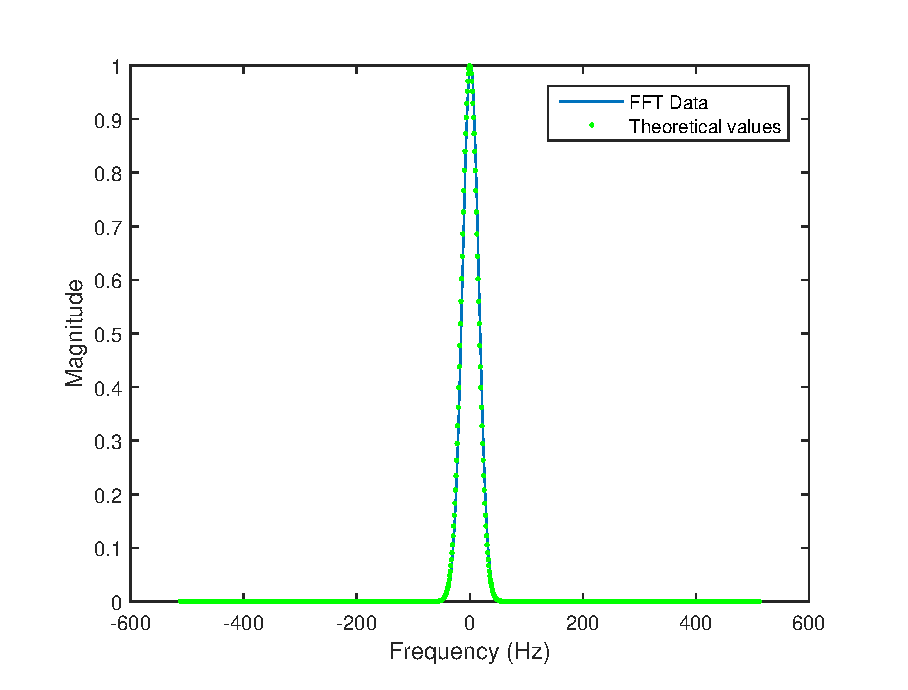
\includegraphics[width=1\textwidth]{../ex1/gaussianFFT}
	\caption{Comparison between the normalized fast fourier transform and the true theoretical fourier transform of the Gaussian (eq. \ref{eq:gaussian})}
	\label{fig:gaussianFFT}
\end{figure}

As we can see in figure \ref{fig:gaussianFFT} the fast fourier transform seem to be pretty spot on. The resolution of the frequencies dependent on the sampling frequency and the amount of samples taken. This because the amount of samples taken directly translates on to how many different frequency values we can get out of the transform\footnote{Due to the linearity of the transform we get one output for each input}. The sample frequency tells us which frequencies we could possibly have caught since one needs two points to capture a period. Basically we have frequencies in the range $[-\frac{1}{2 \Delta},\frac{1}{2 \Delta}]$, where $\Delta$ is the time between samples and since we simulate that we take 1024 samples we get 
\begin{align}
	&(\frac{1}{2 \Delta} +\frac{1}{2 \Delta})/\textit{number of jumps between frequency values} \\ 
	=& (\frac{1}{2\Delta} +\frac{1}{2\Delta})/1023\\
	=& 1024/1023 = 1.001.
\end{align}
This basically means we have 1.001 Hz between the frequencies we get checked in the fourier transform.

\section{The Fourier Transform of a Gaussian}
In this exercise we look at the equation 
\begin{equation}
	u(t) = \bar{u} sin(2 \pi f_c t )
\end{equation}
where $f_c = 8$ and $\bar{u}$ basically is a square wave going between the value 1 and a value $u_1$ which we vary through the exercise. The square wave changes values after a period of the sine function has passed. This is to simulate a message 01010101. Thus we plot the function for one whole time unit. 
\begin{figure}[H]
	\centering
	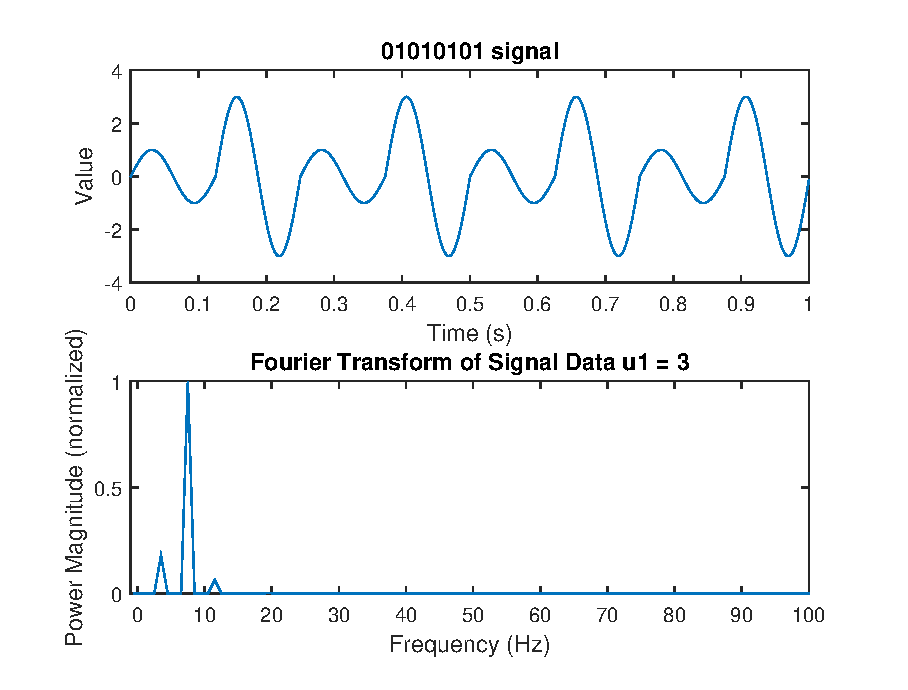
\includegraphics[width=1\textwidth]{../ex2/fftU1-3}
	\caption{Looking at the frequency spectrum of the signal with $u_1 = 3$.}
	\label{fig:fftU1-3}
\end{figure}
\begin{figure}[H]
	\centering
	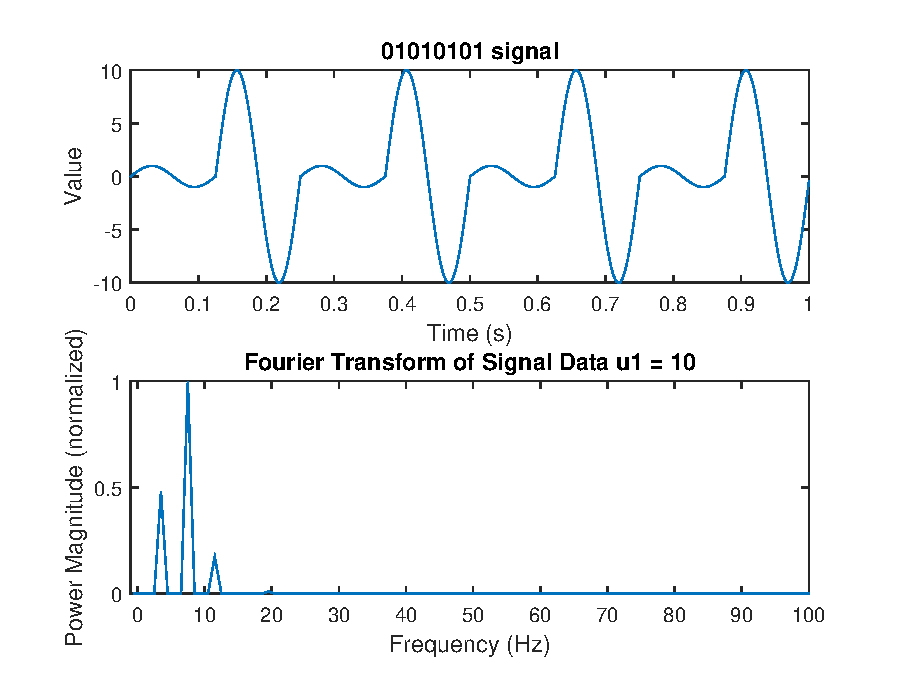
\includegraphics[width=1\textwidth]{../ex2/fftU1-10}
	\caption{Looking at the frequency spectrum of the signal with $u_1 = 10$.}
	\label{fig:fftU1-10}
\end{figure}

\begin{figure}[H]
	\centering
	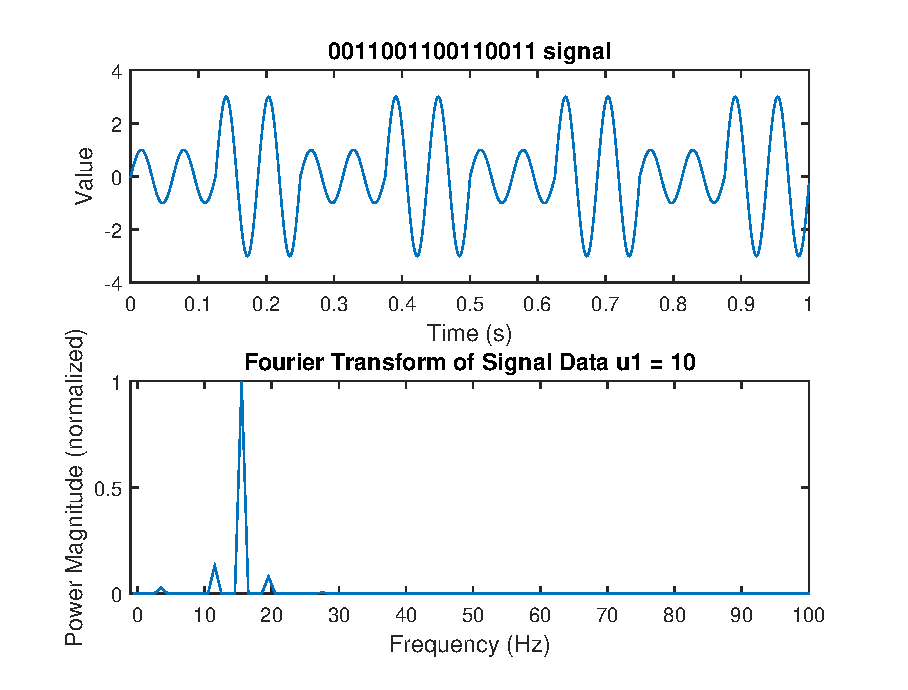
\includegraphics[width=1\textwidth]{../ex2/fftU1-3-double-same}
	\caption{Looking at the frequency spectrum of the signal with $u_1 = 3$. Ontop of that we doubled the carrier frequency without changing the modulation of the sine function. We can see that we have the same bandwidth but the same amount of information is given.}
	\label{fig:fftU1-3}
\end{figure}
\begin{figure}[H]
	\centering
	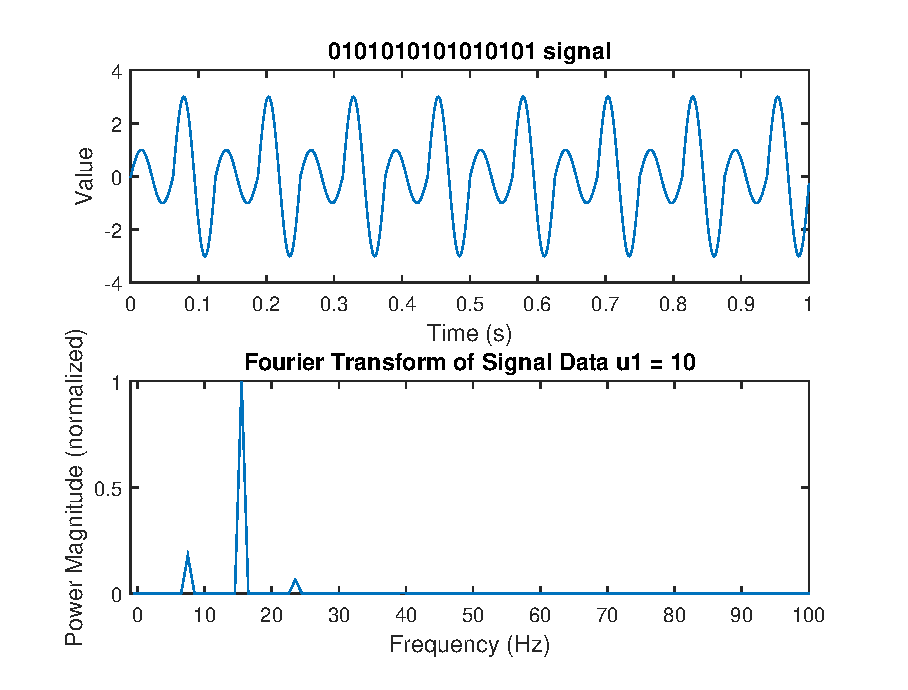
\includegraphics[width=1\textwidth]{../ex2/fftU1-3-double}
	\caption{Looking at the frequency spectrum of the signal with $u_1 = 3$. Ontop of that we double carrier wave frequency and the modulation of the sine function. We can see that we get double the information, at the cost of having a twice as large bandwidth.}
	\label{fig:fftU1-10}
\end{figure}

Looking at figure \ref{fig:fftU1-3} we can see that the frequency bandwidth is 8 Hz (if the time unit is in seconds). Looking at the discussion in the lab instruction about equation (7) in that paper we could perhaps guess the behavior of having  the carrier frequency in the middle of the bandwidth. This because of the centered carrier wave frequency in that case. Here $f_b$ gets to be the square wave instead. That said... it feels slightly like its not a complete connection... only a vague similarity. 

If we increase the value of $u_1$ from 3 to 10 we can see in figure \ref{fig:fftU1-10} that the peaks that corresponds to the square wave gets larger in comparison to the peak that corresponds to the carrier wave. This seems natural since there is a larger effect of the square wave, thus it should get a larger part in the corresponding fourier transform. 

Its interesting to see that if we double the carrier wave frequency and want to send zeros followed by ones, but still be constricted to the same bandwidth, we cant do it. This because if we modulate the sine function faster we get a larger bandwidth. We could however send 0011001100110011 instead of 01010101, but this is not of much interest since its basically the same information. Basically if we change the modulation of the sine function the bandwidth changes. If we increase the modulation we get a larger bandwidth, but can send more information in the same time. If we decrease the modulation we get a smaller bandwidth, but can send less information in the same time. This also seem to depends on each other linearly. 

On a side note one could say that you get double the information since you could count a double zero as a number 2 and a double 1 as a number 3. Ontop of that you could go to 3,4,5,6 zeros and ones and let it signify different values, while still be within the bandwidth. Thus you could push more information through the same bandwidth requirement, by only changing the carrier frequency. 

\newpage
\section{Extracting Information from a Noisy Signal}
In this exercise we simply wanna apply the given gaussian filter onto a given noisy signal. Using this we then wanna decode a bit message in the noisy signal. The signal was given in the file \verb+am26.dat+, and the message was decoded to be \verb+FNM15|jg;.""HAD+. In figure \ref{fig:freqPowSpec} we can see how the signal looks in the fourier space before and after the filter was applied. In figure \ref{fig:signal} we can see how large an impact the filter has onto the original signal. 
\begin{figure}[H]
	\centering
	\newlength\figureheight 
	\newlength\figurewidth 
	\setlength\figureheight{8cm} 
	\setlength\figurewidth{6cm}
	% This file was created by matlab2tikz.
% Minimal pgfplots version: 1.3
%
%The latest updates can be retrieved from
%  http://www.mathworks.com/matlabcentral/fileexchange/22022-matlab2tikz
%where you can also make suggestions and rate matlab2tikz.
%
\definecolor{mycolor1}{rgb}{0.00000,0.44700,0.74100}%
%
\pgfplotsset{every tick label/.append style={font=\tiny}}
\begin{tikzpicture}

\begin{axis}[%
width=0.95092\figurewidth,
height=0.408605\figureheight,
at={(0\figurewidth,0\figureheight)},
scale only axis,
xmin=-5000,
xmax=5000,
xlabel={Frequency (Hz)},
ymin=0,
ymax=5000000,
ylabel={Magnitude},
title style={font=\bfseries},
title={Filtered Frequency Power Spectrum}
]
\addplot [color=mycolor1,solid,forget plot]
  table[row sep=crcr]{%
-4096	0\\
-4095	3583.93340708\\
-4094	1.321889141401e-60\\
-4093	1.61539211458e-59\\
-4092	1.27867639957e-59\\
-4091	1.013426676e-59\\
-4090	2.759383525681e-60\\
-4089	1.745003427316e-60\\
-4088	1.5337681831625e-59\\
-4087	1.35467581525e-59\\
-4086	4.489408648864e-60\\
-4085	3.0746133785e-60\\
-4084	2.99250385501e-59\\
-4083	6.57110158148e-59\\
-4082	7.008050612736e-60\\
-4081	4.86822311644791e-60\\
-4080	2.9438787645e-59\\
-4079	8.6149966977e-59\\
-4078	2.41577406605e-59\\
-4077	2.211874380589e-60\\
-4076	3.99568311801e-59\\
-4075	1.3566149092e-59\\
-4074	1.86433247489e-59\\
-4073	1.54831281451289e-58\\
-4072	7.93358279144e-59\\
-4071	1.230881779625e-58\\
-4070	1.139395812802e-58\\
-4069	3.93233266913e-59\\
-4068	1.127680228516e-58\\
-4067	3.3187637673e-59\\
-4066	3.124192433261e-58\\
-4065	4.3878718589e-58\\
-4064	1.6607753285e-58\\
-4063	2.974477627609e-60\\
-4062	2.25618553e-58\\
-4061	4.60125948639881e-58\\
-4060	4.82358643093e-59\\
-4059	1.027273389701e-58\\
-4058	1.436022094481e-58\\
-4057	1.00281208045e-57\\
-4056	6.381451141876e-58\\
-4055	1.8689658401e-58\\
-4054	3.1743721088e-58\\
-4053	4.849201878176e-58\\
-4052	1.53040974536e-57\\
-4051	4.9183424357e-58\\
-4050	3.09464248141e-57\\
-4049	9.662524574425e-58\\
-4048	2.58275134429e-57\\
-4047	4.96599627325e-59\\
-4046	1.52506259721e-57\\
-4045	2.4554663092196e-57\\
-4044	3.32598239389e-57\\
-4043	5.920003856825e-58\\
-4042	1.84618154632e-57\\
-4041	5.22270466037e-57\\
-4040	3.03328014452e-57\\
-4039	4.54732814842e-57\\
-4038	9.354562516e-59\\
-4037	1.22162684788e-57\\
-4036	1.70170744153e-57\\
-4035	4.5914484032e-57\\
-4034	7.7113240389e-58\\
-4033	6.59837953125e-57\\
-4032	2.1352379172525e-57\\
-4031	3.20969182194e-57\\
-4030	9.94585584682e-57\\
-4029	1.265333067666e-56\\
-4028	2.16677400245e-57\\
-4027	1.700147699281e-56\\
-4026	7.7229374657396e-57\\
-4025	3.52139889652e-57\\
-4024	4.232263539709e-56\\
-4023	1.348304684669e-56\\
-4022	4.2896557448e-57\\
-4021	7.7916147241e-57\\
-4020	2.188724794381e-56\\
-4019	8.75431081928e-57\\
-4018	2.065609818981e-56\\
-4017	1.533366498856e-56\\
-4016	1.01536552345e-55\\
-4015	8.2425815696e-56\\
-4014	3.3664880169e-56\\
-4013	4.001495906641e-56\\
-4012	9.209232207149e-56\\
-4011	7.7120606306e-56\\
-4010	8.012390013136e-56\\
-4009	1.8961512757e-55\\
-4008	1.26364322765e-55\\
-4007	7.11392771156e-57\\
-4006	3.24360055865e-57\\
-4005	1.89377538653e-57\\
-4004	5.6893413589e-57\\
-4003	2.567430977525e-56\\
-4002	9.179880726736e-56\\
-4001	7.356894391321e-56\\
-4000	3.2358705580661e-55\\
-3999	9.1790520872e-56\\
-3998	1.4272399129e-55\\
-3997	3.18653893282e-55\\
-3996	5.05853913546e-55\\
-3995	3.96164342314e-55\\
-3994	3.94158154905e-55\\
-3993	1.23823761074e-55\\
-3992	1.6903145871236e-55\\
-3991	6.13023377265e-55\\
-3990	1.76043553937e-55\\
-3989	6.36274240277e-55\\
-3988	9.7505336773e-56\\
-3987	7.1894391626e-56\\
-3986	8.71563529901e-55\\
-3985	1.586950327456e-54\\
-3984	2.7720963797e-55\\
-3983	4.3180899328421e-55\\
-3982	1.991180368629e-54\\
-3981	7.56616621105e-55\\
-3980	7.59709344661e-55\\
-3979	5.23601222497e-55\\
-3978	9.94046744308e-55\\
-3977	4.23427898165e-55\\
-3976	5.1467293076e-56\\
-3975	2.326455071009e-54\\
-3974	8.80935668253e-55\\
-3973	6.11543997101e-55\\
-3972	5.30541408097e-55\\
-3971	8.7791654421e-54\\
-3970	4.715530852325e-54\\
-3969	3.185903936969e-54\\
-3968	4.457322393061e-54\\
-3967	4.259111080564e-54\\
-3966	2.984174226401e-54\\
-3965	8.1754527121e-54\\
-3964	1.7071712968241e-53\\
-3963	2.492093374189e-54\\
-3962	9.5220306373e-54\\
-3961	2.2026049219989e-53\\
-3960	5.3749903869e-54\\
-3959	3.4870279309529e-53\\
-3958	4.8239187796e-55\\
-3957	3.0605784777236e-53\\
-3956	1.00842224017e-53\\
-3955	2.95855334354e-55\\
-3954	2.4664008032449e-53\\
-3953	3.00411938201e-53\\
-3952	4.60001403364e-53\\
-3951	1.1022239977361e-53\\
-3950	8.5529124293e-54\\
-3949	2.59880577207476e-54\\
-3948	1.130440521757e-52\\
-3947	1.395994269364e-52\\
-3946	6.85564988842e-53\\
-3945	1.65111082277e-53\\
-3944	1.33730907052681e-52\\
-3943	1.087461487108e-52\\
-3942	3.7450231481e-53\\
-3941	2.85086765e-52\\
-3940	9.6182132693e-53\\
-3939	1.244680988405e-52\\
-3938	1.7926624973956e-53\\
-3937	8.33502249457e-53\\
-3936	7.72001737345e-53\\
-3935	8.1350070066109e-53\\
-3934	1.04108059585e-52\\
-3933	2.70926947706e-53\\
-3932	1.791401352625e-52\\
-3931	6.52896592673e-53\\
-3930	4.079127829509e-52\\
-3929	7.256859398401e-52\\
-3928	3.12619065359824e-52\\
-3927	6.3593147984e-52\\
-3926	1.43089791854841e-52\\
-3925	8.88710076116e-53\\
-3924	4.836778361e-52\\
-3923	1.99775343989e-53\\
-3922	4.664972817781e-52\\
-3921	9.2046821569e-52\\
-3920	9.6561805761e-52\\
-3919	2.84202528433616e-52\\
-3918	1.89847722485e-53\\
-3917	2.597030469125e-52\\
-3916	5.535763758421e-52\\
-3915	7.193963079229e-52\\
-3914	3.546083466704e-52\\
-3913	4.337193467664e-52\\
-3912	2.3063710865e-52\\
-3911	5.3030249285e-52\\
-3910	1.1765883830425e-51\\
-3909	1.4322000788e-51\\
-3908	5.704827889076e-52\\
-3907	1.82391960874e-51\\
-3906	4.193199126324e-52\\
-3905	2.6268637933e-53\\
-3904	1.26115063204e-51\\
-3903	5.7359947333e-52\\
-3902	3.2500052978121e-51\\
-3901	4.11358330154e-51\\
-3900	1.969340809e-51\\
-3899	1.4249023311956e-51\\
-3898	2.36219743493e-51\\
-3897	1.203464006585e-52\\
-3896	1.69068489245e-51\\
-3895	1.4398454730664e-51\\
-3894	2.81426525965e-51\\
-3893	5.20679101805e-51\\
-3892	4.59594033449e-51\\
-3891	5.9597030084e-52\\
-3890	1.5303784576e-51\\
-3889	1.56381536276e-51\\
-3888	2.6969722369e-51\\
-3887	1.179625921938e-50\\
-3886	1.1889846851984e-51\\
-3885	5.14705293953e-51\\
-3884	1.076300367397e-50\\
-3883	1.1013564026e-50\\
-3882	2.8812976517e-50\\
-3881	7.26712024405e-51\\
-3880	6.6173076311581e-51\\
-3879	5.96754989018e-51\\
-3878	3.322744249576e-50\\
-3877	2.9853606725e-51\\
-3876	2.20587197065e-51\\
-3875	5.2743729361e-51\\
-3874	1.694571779344e-50\\
-3873	4.0894302265e-50\\
-3872	3.844850195189e-50\\
-3871	1.784787705424e-50\\
-3870	1.041851527897e-50\\
-3869	2.179593170564e-50\\
-3868	2.460989996996e-50\\
-3867	4.94903220551849e-50\\
-3866	2.1203112341e-50\\
-3865	1.7694022385e-50\\
-3864	6.40282044706e-51\\
-3863	4.10365546e-50\\
-3862	3.527997763501e-50\\
-3861	2.8668578363401e-49\\
-3860	1.140779111636e-50\\
-3859	8.97354007777e-51\\
-3858	7.5896043065e-50\\
-3857	2.50541848453e-49\\
-3856	1.01260150765444e-51\\
-3855	9.423163796e-50\\
-3854	9.2394705933e-50\\
-3853	2.185973600296e-50\\
-3852	1.3638813250724e-49\\
-3851	1.8464892634989e-49\\
-3850	2.02214873453e-49\\
-3849	4.84415893249e-49\\
-3848	4.67441378944e-49\\
-3847	1.810197647824e-50\\
-3846	2.859068822161e-50\\
-3845	5.0068307405e-50\\
-3844	4.023458585161e-50\\
-3843	3.17948544745e-49\\
-3842	3.0694916621e-49\\
-3841	1.517585079581e-48\\
-3840	1.690839971444e-50\\
-3839	3.88398741844e-49\\
-3838	5.13923149697e-49\\
-3837	9.83204640925e-49\\
-3836	3.90482651594e-49\\
-3835	5.70110516537e-49\\
-3834	6.1154825405e-49\\
-3833	4.59006805997e-49\\
-3832	1.01173144868249e-48\\
-3831	7.07578561296e-49\\
-3830	1.9159609691456e-49\\
-3829	1.894714121444e-48\\
-3828	1.764484019792e-48\\
-3827	5.4072381056e-50\\
-3826	7.8478807325e-49\\
-3825	1.03957334372e-49\\
-3824	3.54710674856e-49\\
-3823	2.9385409825325e-49\\
-3822	1.3265798564e-48\\
-3821	6.55675441172e-49\\
-3820	4.21467146425e-49\\
-3819	6.949778305e-48\\
-3818	6.7924515205796e-49\\
-3817	3.897527601056e-48\\
-3816	3.9457940264e-48\\
-3815	2.474238995101e-48\\
-3814	4.300022904421e-48\\
-3813	1.243299060994e-48\\
-3812	7.924428692849e-48\\
-3811	7.3272887234e-48\\
-3810	4.71446175265e-49\\
-3809	4.975429584229e-48\\
-3808	5.532544882976e-48\\
-3807	6.6620399624e-48\\
-3806	1.11732387005e-47\\
-3805	1.2831620842e-47\\
-3804	1.70984370824e-47\\
-3803	5.653187813821e-48\\
-3802	1.1677310521e-47\\
-3801	5.451356926804e-48\\
-3800	9.3226171025e-48\\
-3799	1.18461952585e-47\\
-3798	4.94594183266e-47\\
-3797	4.133192925761e-48\\
-3796	2.25167962034e-47\\
-3795	9.07487710345e-49\\
-3794	1.40962657587921e-47\\
-3793	1.47616434277e-47\\
-3792	2.8087036372e-47\\
-3791	1.10830432313e-47\\
-3790	6.4652219791549e-47\\
-3789	1.47169831426e-47\\
-3788	1.04927694976e-47\\
-3787	9.456737901025e-48\\
-3786	2.18534196177e-47\\
-3785	2.62349323661e-47\\
-3784	4.20704762837e-47\\
-3783	3.89650739813e-47\\
-3782	3.81479813482e-47\\
-3781	1.0455064618e-46\\
-3780	3.27985750762e-47\\
-3779	2.302854056721e-46\\
-3778	2.59682049604e-47\\
-3777	5.74296138916e-47\\
-3776	6.4119008936e-48\\
-3775	2.323762700221e-46\\
-3774	4.47322834625e-47\\
-3773	1.0264880277584e-47\\
-3772	1.145803334929e-46\\
-3771	4.37646849505e-47\\
-3770	2.157417078089e-46\\
-3769	7.9971123188329e-47\\
-3768	8.7263564521941e-47\\
-3767	1.51449719149e-47\\
-3766	8.8604393e-48\\
-3765	8.50432549157e-47\\
-3764	5.3066509549569e-47\\
-3763	4.306504526389e-46\\
-3762	4.586374870376e-46\\
-3761	1.17576309152e-47\\
-3760	2.3347456442756e-47\\
-3759	8.478591496e-47\\
-3758	1.725664495169e-46\\
-3757	6.83908865226e-47\\
-3756	1.2970594439764e-47\\
-3755	3.9530717714e-46\\
-3754	6.87983495018e-47\\
-3753	4.8391323381e-47\\
-3752	1.252303829753e-46\\
-3751	4.1411989898e-46\\
-3750	4.0917141577e-46\\
-3749	2.72199445982784e-46\\
-3748	4.187521242769e-46\\
-3747	2.9459556242e-47\\
-3746	2.573410179509e-46\\
-3745	5.328891938276e-46\\
-3744	2.1547176573521e-45\\
-3743	4.023516742664e-46\\
-3742	1.60800890338e-45\\
-3741	1.63004808125e-47\\
-3740	2.588501906901e-46\\
-3739	7.4559033925e-46\\
-3738	6.460556854564e-46\\
-3737	8.950837153e-46\\
-3736	2.4201301875316e-45\\
-3735	2.5580673962125e-45\\
-3734	1.67331652765e-45\\
-3733	1.537230322649e-46\\
-3732	9.313772523336e-46\\
-3731	9.25138443177e-45\\
-3730	3.44087521021e-45\\
-3729	2.43059648705e-45\\
-3728	1.71099951519033e-45\\
-3727	1.9075649090741e-45\\
-3726	7.381634606344e-46\\
-3725	6.33689547173e-45\\
-3724	2.19687978833e-45\\
-3723	7.77175164497e-45\\
-3722	4.82985256729e-45\\
-3721	2.828834395325e-46\\
-3720	3.81901312233002e-45\\
-3719	2.92761919885e-45\\
-3718	3.70276753985e-45\\
-3717	9.7222240601e-46\\
-3716	7.6343390545e-46\\
-3715	8.22951374717e-45\\
-3714	8.35681697401e-45\\
-3713	1.18274375417e-45\\
-3712	1.626665913941e-44\\
-3711	7.105065181381e-46\\
-3710	4.56852275521e-45\\
-3709	4.25691435997721e-46\\
-3708	5.9066235144104e-45\\
-3707	2.023146366356e-44\\
-3706	4.5871062634e-45\\
-3705	1.843371108829e-44\\
-3704	6.5420830336e-46\\
-3703	1.596644833841e-44\\
-3702	2.036549374801e-46\\
-3701	3.639872010289e-44\\
-3700	1.921799708021e-44\\
-3699	6.518100279364e-44\\
-3698	3.808733357169e-44\\
-3697	3.84943752205e-45\\
-3696	5.5465465217e-46\\
-3695	1.09315775816e-43\\
-3694	9.6556091245e-44\\
-3693	1.1329808857e-45\\
-3692	2.99678689864129e-44\\
-3691	1.052646588097e-44\\
-3690	8.3573382113e-44\\
-3689	1.161994357376e-44\\
-3688	7.9436620754e-44\\
-3687	6.863275005584e-44\\
-3686	1.743020877749e-44\\
-3685	1.6530426119069e-43\\
-3684	1.1057394554e-44\\
-3683	4.421138908909e-44\\
-3682	8.334742089616e-44\\
-3681	3.67901709361e-45\\
-3680	6.1388116996e-44\\
-3679	9.018478596629e-44\\
-3678	1.22837979976422e-43\\
-3677	2.12718494722e-43\\
-3676	2.49798494228e-43\\
-3675	8.25927531722e-43\\
-3674	2.64066683065e-43\\
-3673	1.48423866169e-43\\
-3672	1.14560230628816e-44\\
-3671	5.77453479364e-45\\
-3670	2.67197562085e-43\\
-3669	1.01923530356e-45\\
-3668	2.7664498975349e-43\\
-3667	4.1312081101e-43\\
-3666	1.0713081514e-42\\
-3665	7.2741372626e-44\\
-3664	7.89500333785e-43\\
-3663	7.68720396377e-43\\
-3662	6.31520655588e-43\\
-3661	8.63641271413e-43\\
-3660	2.82697663613e-43\\
-3659	5.60776452905e-43\\
-3658	8.1242893418e-43\\
-3657	1.834381886229e-42\\
-3656	5.0629738865e-42\\
-3655	1.765431940625e-42\\
-3654	2.38645863145e-43\\
-3653	2.8425185081e-42\\
-3652	2.257935545489e-42\\
-3651	3.316365271525e-42\\
-3650	2.276848707949e-42\\
-3649	2.550519521936e-42\\
-3648	8.37350679425e-43\\
-3647	1.10301276090625e-42\\
-3646	2.453099417e-44\\
-3645	2.4993662887661e-43\\
-3644	3.822730060409e-42\\
-3643	4.2191171138e-42\\
-3642	7.5845813801e-42\\
-3641	4.302427298756e-42\\
-3640	1.884458375489e-42\\
-3639	9.4041083734949e-43\\
-3638	1.69109561666e-41\\
-3637	5.352717430724e-42\\
-3636	7.180303623809e-42\\
-3635	7.2205156692e-42\\
-3634	2.830879805e-42\\
-3633	1.02070259378064e-42\\
-3632	6.552568483609e-42\\
-3631	3.1666628818849e-41\\
-3630	1.0722780015376e-41\\
-3629	2.08984093953769e-42\\
-3628	7.9248088453e-42\\
-3627	8.11109319368e-41\\
-3626	4.3202761157e-42\\
-3625	3.484567931156e-42\\
-3624	8.03395208585e-41\\
-3623	7.9922547202384e-43\\
-3622	2.2730022831816e-41\\
-3621	6.2393188388e-41\\
-3620	9.193314825689e-42\\
-3619	4.30871984953e-41\\
-3618	2.83018377508e-41\\
-3617	1.84902794704e-41\\
-3616	2.07716634962594e-41\\
-3615	7.423772186129e-42\\
-3614	4.95676509562e-41\\
-3613	1.027190459321e-40\\
-3612	1.756496086344e-40\\
-3611	9.9913405793e-41\\
-3610	9.1885534029e-42\\
-3609	5.1152129614144e-41\\
-3608	5.54709262297e-41\\
-3607	2.610443245e-41\\
-3606	1.096890639169e-40\\
-3605	1.65550186322e-41\\
-3604	1.062410381064e-40\\
-3603	5.14908597226e-41\\
-3602	1.03176038761e-41\\
-3601	5.6005713625e-41\\
-3600	4.68697585993e-41\\
-3599	1.740886636325e-40\\
-3598	3.0465445426e-42\\
-3597	5.286435220025e-40\\
-3596	5.95890445613e-41\\
-3595	1.835798317189e-42\\
-3594	2.570189553256e-40\\
-3593	2.650191064384e-40\\
-3592	1.64372320625e-41\\
-3591	4.13305759969e-41\\
-3590	2.483912824516e-40\\
-3589	3.897280750324e-40\\
-3588	2.091162622889e-40\\
-3587	8.796807303876e-40\\
-3586	1.1775415077001e-41\\
-3585	5.8887400725e-40\\
-3584	1.0339612704e-41\\
-3583	5.16500124845e-41\\
-3582	1.590543239869e-40\\
-3581	9.245428112e-40\\
-3580	8.6387411714e-42\\
-3579	2.411215604125e-40\\
-3578	1.0412894593025e-39\\
-3577	7.10898686577e-41\\
-3576	4.04404035009056e-40\\
-3575	9.24046174994e-41\\
-3574	3.799144318921e-42\\
-3573	2.468015709625e-40\\
-3572	2.421853142696e-40\\
-3571	6.91798675465e-41\\
-3570	1.594037103572e-40\\
-3569	3.6406153989e-40\\
-3568	1.89515743037e-39\\
-3567	5.97875315381e-39\\
-3566	3.1541346965e-40\\
-3565	7.765577255176e-40\\
-3564	5.0866842148e-40\\
-3563	7.092070962484e-40\\
-3562	3.00025459961e-39\\
-3561	6.1369094056e-40\\
-3560	2.2881438414469e-39\\
-3559	7.90628551336864e-40\\
-3558	4.46324722724e-39\\
-3557	8.59703997685e-39\\
-3556	1.12624121888e-39\\
-3555	7.24850386408e-39\\
-3554	5.75855799592e-41\\
-3553	1.16916252274e-39\\
-3552	1.9346693913e-39\\
-3551	7.09674301561e-39\\
-3550	3.14337735493e-39\\
-3549	1.835011137625e-40\\
-3548	5.2396211449e-39\\
-3547	6.85809476738e-39\\
-3546	8.47344980225e-39\\
-3545	2.16306461729e-39\\
-3544	3.34086792777e-39\\
-3543	1.325845609281e-38\\
-3542	2.8653113809e-39\\
-3541	4.79221984573e-39\\
-3540	1.999866553544e-38\\
-3539	1.119517789417e-38\\
-3538	7.05342235021e-39\\
-3537	4.57975611424e-39\\
-3536	2.1254348882e-38\\
-3535	2.9612236709e-38\\
-3534	1.141378552836e-38\\
-3533	3.1297339765e-38\\
-3532	1.06035260413e-38\\
-3531	4.4974279849e-38\\
-3530	3.693844441625e-38\\
-3529	3.58757290697e-39\\
-3528	2.982970704661e-38\\
-3527	1.6553138055444e-39\\
-3526	7.3091023945e-38\\
-3525	1.703428648281e-38\\
-3524	3.91537837634e-39\\
-3523	3.472377820084e-38\\
-3522	3.8106184832e-38\\
-3521	1.321541628244e-38\\
-3520	5.569846724e-38\\
-3519	9.731549565749e-38\\
-3518	3.425546123156e-38\\
-3517	4.270632062021e-38\\
-3516	3.513359034056e-38\\
-3515	5.000539234e-38\\
-3514	1.240073537716e-38\\
-3513	1.22172780985e-38\\
-3512	8.7896577908e-38\\
-3511	7.64417747668081e-38\\
-3510	8.3279601649e-38\\
-3509	1.07741494560544e-38\\
-3508	7.0103573044e-38\\
-3507	1.12251007237e-37\\
-3506	5.5132896881e-38\\
-3505	2.084244119609e-38\\
-3504	1.53383045161e-37\\
-3503	2.25654256305e-37\\
-3502	6.2195400202e-38\\
-3501	1.402363157156e-38\\
-3500	8.388896558125e-38\\
-3499	4.503594355101e-38\\
-3498	1.16582050234e-37\\
-3497	1.16590259336e-37\\
-3496	6.28023564232e-37\\
-3495	1.44213299541e-37\\
-3494	1.40170737177e-37\\
-3493	1.63871015332e-37\\
-3492	1.0118974363496e-37\\
-3491	7.171416953e-37\\
-3490	6.1627612188169e-37\\
-3489	9.615686499361e-38\\
-3488	2.3002272389e-37\\
-3487	3.9123803423601e-37\\
-3486	2.7260590754e-36\\
-3485	1.2768560081e-37\\
-3484	9.2244367154e-38\\
-3483	5.662530235249e-38\\
-3482	1.115868469e-37\\
-3481	3.09628936864025e-36\\
-3480	5.547761342084e-36\\
-3479	4.91642648885e-37\\
-3478	2.756072468836e-36\\
-3477	3.7155388073e-36\\
-3476	2.522623914049e-36\\
-3475	4.6437199441e-37\\
-3474	1.493915288144e-36\\
-3473	3.926859823796e-36\\
-3472	3.210399473476e-36\\
-3471	9.55511435476e-37\\
-3470	3.95695673866e-37\\
-3469	4.96462482e-36\\
-3468	5.005516473796e-36\\
-3467	3.3370160509264e-37\\
-3466	5.172640138025e-36\\
-3465	2.258315138e-36\\
-3464	4.48671530405e-37\\
-3463	2.963524330141e-36\\
-3462	4.5628228133e-37\\
-3461	6.3266028904e-36\\
-3460	2.37180667895604e-36\\
-3459	2.5869808106e-36\\
-3458	3.01285298097e-35\\
-3457	3.425450897261e-36\\
-3456	1.72387622603225e-36\\
-3455	4.9997112388e-36\\
-3454	2.216869295801e-36\\
-3453	9.8593682938e-36\\
-3452	1.1724817757e-35\\
-3451	3.7898679656e-36\\
-3450	1.20617671396e-35\\
-3449	3.236584240741e-36\\
-3448	4.5621193928e-36\\
-3447	1.12372944203202e-35\\
-3446	2.944785470021e-36\\
-3445	3.62827802129e-35\\
-3444	7.2805159674e-36\\
-3443	9.7895350697e-36\\
-3442	3.644961316e-36\\
-3441	3.35546620301e-35\\
-3440	2.3489443059784e-35\\
-3439	3.910649013181e-36\\
-3438	1.58948543312e-35\\
-3437	2.43490895077e-35\\
-3436	8.91200710889e-35\\
-3435	2.4755149985e-35\\
-3434	1.03293738725e-35\\
-3433	6.85846841137e-35\\
-3432	2.6504734376e-35\\
-3431	3.326922040384e-36\\
-3430	2.5224295087364e-35\\
-3429	5.38467411481e-35\\
-3428	4.87995243073e-35\\
-3427	8.50265426393e-35\\
-3426	6.9294533629e-36\\
-3425	1.444781861021e-34\\
-3424	1.24348829045e-35\\
-3423	1.34179187746e-35\\
-3422	1.9350755716e-35\\
-3421	2.0169571736896e-35\\
-3420	7.87890846573e-35\\
-3419	7.5623244437824e-35\\
-3418	2.55641504065e-35\\
-3417	3.90909730762e-35\\
-3416	1.496486079625e-36\\
-3415	1.123070796445e-34\\
-3414	8.84533531808e-35\\
-3413	1.49721677485e-35\\
-3412	5.7251136085e-36\\
-3411	1.402651557721e-34\\
-3410	9.73788438346e-35\\
-3409	4.581122229e-35\\
-3408	1.569664475789e-34\\
-3407	4.178613674e-34\\
-3406	3.36638706714601e-34\\
-3405	6.564533972441e-34\\
-3404	2.80083962e-34\\
-3403	2.095001092225e-34\\
-3402	8.4261463849e-34\\
-3401	8.2916632917e-34\\
-3400	9.116563048e-34\\
-3399	4.39442878586e-35\\
-3398	7.30551977153e-35\\
-3397	5.7472956445e-34\\
-3396	4.644588121636e-36\\
-3395	1.36068994477e-33\\
-3394	2.130062265425e-34\\
-3393	3.2719064962e-34\\
-3392	5.0899430405e-34\\
-3391	1.21728639797e-33\\
-3390	1.508479184689e-34\\
-3389	1.74644148501225e-34\\
-3388	4.790614195429e-34\\
-3387	5.9050310345e-34\\
-3386	2.31720087409e-35\\
-3385	4.473831637764e-34\\
-3384	7.0665788125e-34\\
-3383	3.377419260004e-34\\
-3382	1.765646007305e-34\\
-3381	1.19652075605e-33\\
-3380	3.854548538996e-34\\
-3379	1.35574968757609e-34\\
-3378	1.5519187872401e-33\\
-3377	6.1488934789e-34\\
-3376	3.27028692509e-33\\
-3375	2.61209470372e-33\\
-3374	1.586456564584e-34\\
-3373	2.3994961954e-34\\
-3372	5.88050360937e-33\\
-3371	5.168733839125e-34\\
-3370	4.268746014449e-34\\
-3369	1.2342153248e-33\\
-3368	3.245440875641e-34\\
-3367	1.902163891069e-34\\
-3366	1.56567316278224e-34\\
-3365	1.70997764625e-33\\
-3364	7.227572475825e-34\\
-3363	4.4730441416e-33\\
-3362	1.7479092974644e-33\\
-3361	3.26002627625e-33\\
-3360	1.83611748137e-33\\
-3359	3.35302760561e-33\\
-3358	6.37874022109e-33\\
-3357	3.8440884169e-33\\
-3356	1.40152644644e-33\\
-3355	1.2792998445184e-33\\
-3354	7.0627907299381e-33\\
-3353	6.4556678065e-34\\
-3352	6.980478941e-33\\
-3351	7.44362472481e-33\\
-3350	4.5779256081e-33\\
-3349	1.10664738468e-33\\
-3348	2.97738013729e-33\\
-3347	7.30827684484e-33\\
-3346	9.3531023314e-34\\
-3345	4.8841472277e-33\\
-3344	2.72002933978e-33\\
-3343	5.3316423829e-34\\
-3342	5.82985974625e-33\\
-3341	3.8080696162e-32\\
-3340	1.170139797225e-32\\
-3339	5.82344363296e-33\\
-3338	3.047812268084e-32\\
-3337	3.79726616285e-33\\
-3336	3.09292721138e-33\\
-3335	4.4562594169741e-33\\
-3334	2.890499629225e-32\\
-3333	4.98711121929e-33\\
-3332	6.28284065005e-33\\
-3331	9.45765528244e-33\\
-3330	1.9862441103609e-33\\
-3329	3.9540782021e-32\\
-3328	3.336035157909e-32\\
-3327	4.2756154165e-32\\
-3326	1.5819855547581e-33\\
-3325	1.949429032625e-32\\
-3324	1.31014697018e-32\\
-3323	1.07158064522e-31\\
-3322	6.8690568410621e-33\\
-3321	6.328082545076e-32\\
-3320	1.96185729037e-33\\
-3319	7.1214557258e-32\\
-3318	1.2312790746244e-31\\
-3317	9.1342919005e-32\\
-3316	5.36868112889e-33\\
-3315	3.739148000101e-32\\
-3314	6.133454068264e-32\\
-3313	4.14211150097876e-32\\
-3312	2.3001595057796e-31\\
-3311	4.3283613545e-32\\
-3310	6.2206311632e-32\\
-3309	2.494595628689e-32\\
-3308	8.987152198921e-32\\
-3307	1.232170742249e-32\\
-3306	2.382819471364e-32\\
-3305	1.71380090997e-31\\
-3304	5.326269043104e-32\\
-3303	8.5918213133e-32\\
-3302	9.16079591969e-33\\
-3301	7.2595291752e-32\\
-3300	8.43218029265e-31\\
-3299	2.4159590522e-31\\
-3298	8.5209609276389e-33\\
-3297	2.83536380264e-31\\
-3296	3.73009623589e-31\\
-3295	1.030632309748e-30\\
-3294	8.4738392469e-33\\
-3293	5.01686491385e-31\\
-3292	4.5782902538e-32\\
-3291	5.49194154484e-31\\
-3290	3.247132587781e-32\\
-3289	1.363874758625e-30\\
-3288	6.89896935556e-31\\
-3287	6.1006817963176e-31\\
-3286	2.652683240629e-30\\
-3285	5.1798925457e-32\\
-3284	9.97061897401e-31\\
-3283	5.98150146625e-31\\
-3282	4.89125298922e-31\\
-3281	4.88693142101e-31\\
-3280	5.16348265277e-31\\
-3279	2.161620675125e-30\\
-3278	5.70392281693e-31\\
-3277	1.004956167409e-30\\
-3276	6.80691476818e-31\\
-3275	1.064806688116e-30\\
-3274	8.44960335524e-31\\
-3273	3.4775158225e-30\\
-3272	9.02933832701e-31\\
-3271	8.57056300288e-31\\
-3270	3.088846015956e-30\\
-3269	3.64405597893796e-30\\
-3268	2.483127207625e-30\\
-3267	4.34873309224e-31\\
-3266	2.41805806800896e-32\\
-3265	2.820111830429e-30\\
-3264	3.3543644005e-30\\
-3263	9.925788367125e-30\\
-3262	5.657969902069e-30\\
-3261	1.73660340712e-29\\
-3260	4.3742526353e-30\\
-3259	1.087979322978e-30\\
-3258	1.1598204285e-29\\
-3257	6.874048179044e-30\\
-3256	8.569122775421e-30\\
-3255	2.1971623552e-29\\
-3254	1.30547558539801e-30\\
-3253	1.8681845878664e-29\\
-3252	7.24454445794e-31\\
-3251	1.138551864305e-30\\
-3250	2.46316755088e-29\\
-3249	9.65312318106e-31\\
-3248	1.9517275282e-29\\
-3247	8.4791101586e-32\\
-3246	1.71156016586e-31\\
-3245	1.54442773082e-29\\
-3244	6.975326375981e-30\\
-3243	7.79153641965e-29\\
-3242	5.5829446402e-30\\
-3241	1.7385848345e-29\\
-3240	2.91767083769e-29\\
-3239	2.88794181241e-29\\
-3238	5.02621182377e-29\\
-3237	7.075545679681e-30\\
-3236	1.90376255602e-29\\
-3235	6.8348438885e-30\\
-3234	6.3985392929e-29\\
-3233	3.9115821765341e-29\\
-3232	3.08075879645e-29\\
-3231	5.196236688449e-30\\
-3230	5.87000058577e-29\\
-3229	1.020957562321e-28\\
-3228	3.005736016901e-28\\
-3227	1.01336968226e-29\\
-3226	1.831065098084e-28\\
-3225	6.55856032122e-29\\
-3224	1.429563648725e-30\\
-3223	4.59482956605e-29\\
-3222	7.35513825493e-29\\
-3221	4.8425905714e-28\\
-3220	2.5821428924141e-29\\
-3219	2.012619748849e-28\\
-3218	2.034683976209e-28\\
-3217	2.4588883981e-28\\
-3216	1.766186862856e-28\\
-3215	5.526398497876e-28\\
-3214	2.2248665465e-28\\
-3213	2.223542921236e-28\\
-3212	6.347917678681e-28\\
-3211	1.430951679365e-28\\
-3210	4.016158637156e-28\\
-3209	1.821568073021e-28\\
-3208	4.134330623641e-28\\
-3207	3.2813084005e-28\\
-3206	3.9528557492e-28\\
-3205	1.2393485923309e-29\\
-3204	1.20765567135044e-28\\
-3203	4.122721985821e-28\\
-3202	9.75152859701e-29\\
-3201	2.131387119625e-30\\
-3200	9.0464148125e-28\\
-3199	8.4169616544e-29\\
-3198	2.637425108729e-28\\
-3197	2.456585896861e-28\\
-3196	3.128457211024e-28\\
-3195	1.15640654984e-27\\
-3194	7.7168974007701e-29\\
-3193	2.797715062609e-28\\
-3192	1.50959933968e-27\\
-3191	4.072970491189e-28\\
-3190	7.0683019178e-28\\
-3189	4.584134462324e-28\\
-3188	6.841741861e-29\\
-3187	1.466196464621e-28\\
-3186	2.79348709874e-27\\
-3185	2.939657322649e-28\\
-3184	6.49079783509e-27\\
-3183	2.6638709477e-28\\
-3182	8.03511418408969e-28\\
-3181	9.8169713897e-28\\
-3180	5.34810462218e-27\\
-3179	4.12538681092e-27\\
-3178	4.22346330365e-27\\
-3177	1.89798875801e-27\\
-3176	6.91106243921e-27\\
-3175	4.74908426525e-27\\
-3174	5.4141393748e-28\\
-3173	1.0015435525e-27\\
-3172	8.26206491749e-27\\
-3171	3.01901486329e-27\\
-3170	3.3200295833e-27\\
-3169	3.10880026708e-27\\
-3168	5.023401697156e-28\\
-3167	9.45169236749e-27\\
-3166	1.101343392209e-26\\
-3165	6.36977571893e-27\\
-3164	3.57395870269e-27\\
-3163	1.2799185761e-26\\
-3162	3.166779189069e-28\\
-3161	5.63070542868e-27\\
-3160	1.161029362e-26\\
-3159	2.3934382501e-26\\
-3158	4.69633316165e-27\\
-3157	3.7422625045e-27\\
-3156	4.47762246922e-27\\
-3155	7.51349828034e-27\\
-3154	2.049802538824e-26\\
-3153	5.7780020752e-27\\
-3152	1.6301146901e-26\\
-3151	5.4484445797209e-27\\
-3150	4.6537538114e-28\\
-3149	6.41732312957e-27\\
-3148	9.61544395925e-27\\
-3147	6.712537677949e-26\\
-3146	1.722735475364e-26\\
-3145	4.135120065869e-26\\
-3144	1.150202362916e-26\\
-3143	1.1243498209924e-25\\
-3142	2.172160405829e-26\\
-3141	7.316843966224e-26\\
-3140	5.76507586978e-27\\
-3139	4.738659742836e-28\\
-3138	2.635870274804e-26\\
-3137	7.366338809e-26\\
-3136	5.29422892402441e-26\\
-3135	5.9460184625e-26\\
-3134	6.245905482536e-26\\
-3133	1.0881003410329e-25\\
-3132	5.939844665269e-26\\
-3131	6.2550673825e-26\\
-3130	8.2850007314e-26\\
-3129	4.021279948825e-26\\
-3128	1.0954478152e-25\\
-3127	1.24628511049e-25\\
-3126	2.11283334341e-27\\
-3125	7.88324300725e-27\\
-3124	8.848855024756e-26\\
-3123	5.830903221669e-26\\
-3122	6.47898298372e-27\\
-3121	4.38466955552e-27\\
-3120	8.7512227657e-26\\
-3119	5.10964101828e-27\\
-3118	2.34825969577e-25\\
-3117	1.0230813520544e-25\\
-3116	3.670924904296e-26\\
-3115	1.79018470682e-25\\
-3114	1.226216901325e-26\\
-3113	1.47650976218e-25\\
-3112	6.6646173796e-26\\
-3111	5.6709356562e-26\\
-3110	1.17896002361e-25\\
-3109	7.5852745821e-26\\
-3108	1.26446075389e-25\\
-3107	5.24468231821e-25\\
-3106	5.3344945201e-27\\
-3105	1.9123778617541e-25\\
-3104	8.28072225045e-25\\
-3103	1.35482249825e-25\\
-3102	5.86604929738e-25\\
-3101	1.4872763585e-25\\
-3100	9.338298141344e-26\\
-3099	6.59803170128e-25\\
-3098	5.6829061736e-25\\
-3097	1.11397689125e-25\\
-3096	1.2982795524139e-25\\
-3095	6.36451069988e-25\\
-3094	7.650744360869e-26\\
-3093	2.481770968741e-26\\
-3092	1.95689866149e-25\\
-3091	7.21527487972e-25\\
-3090	5.5818662288e-25\\
-3089	3.69198400825e-25\\
-3088	9.68541858058e-25\\
-3087	1.6330595708584e-25\\
-3086	3.733963186e-25\\
-3085	4.892007598325e-26\\
-3084	5.647417540949e-26\\
-3083	7.67128448808e-25\\
-3082	5.66627974837e-25\\
-3081	1.218476154913e-24\\
-3080	1.297905913825e-24\\
-3079	6.76692378545e-25\\
-3078	7.60282928785e-25\\
-3077	3.91034982377e-25\\
-3076	9.27604064269e-25\\
-3075	1.475735350304e-24\\
-3074	4.3813839554344e-25\\
-3073	1.875314264104e-24\\
-3072	6.1116562445e-25\\
-3071	2.41474102484e-25\\
-3070	1.000312848874e-24\\
-3069	1.022399931089e-24\\
-3068	2.310181554564e-24\\
-3067	4.70363238001e-25\\
-3066	3.04562862533e-25\\
-3065	4.871057918116e-26\\
-3064	4.4442052212776e-25\\
-3063	3.425487602949e-24\\
-3062	1.849140396496e-24\\
-3061	2.16413051186e-25\\
-3060	6.053599845e-26\\
-3059	5.8776341746e-25\\
-3058	1.923550032836e-24\\
-3057	1.021760512754e-24\\
-3056	3.0970703529e-24\\
-3055	1.541512883305e-24\\
-3054	7.06375379385e-25\\
-3053	2.9989632385e-24\\
-3052	1.91156383354e-25\\
-3051	2.47960577237e-25\\
-3050	1.1882310184e-25\\
-3049	2.412523772509e-24\\
-3048	1.33530709441e-25\\
-3047	1.998448247449e-24\\
-3046	2.28025715333e-25\\
-3045	3.342124696144e-24\\
-3044	4.088509117576e-24\\
-3043	1.1022178759429e-23\\
-3042	6.654387707444e-24\\
-3041	1.33381766873705e-24\\
-3040	4.22934711986e-25\\
-3039	7.0691966948e-24\\
-3038	2.434048540369e-24\\
-3037	1.52850838213e-23\\
-3036	1.21497281722e-23\\
-3035	6.244869706661e-24\\
-3034	3.90464319925e-25\\
-3033	4.810096202981e-24\\
-3032	1.0052035028e-23\\
-3031	7.7085280093e-24\\
-3030	5.282792999721e-24\\
-3029	3.09241693328e-25\\
-3028	2.55381113637e-23\\
-3027	7.7762480962e-24\\
-3026	6.443872990244e-24\\
-3025	1.2847725284e-23\\
-3024	2.41813727581e-23\\
-3023	3.5202422504e-23\\
-3022	2.73694544549e-23\\
-3021	1.0733798617e-23\\
-3020	1.57944660256e-23\\
-3019	2.43793772365e-23\\
-3018	2.7878594549e-23\\
-3017	3.48965238925e-23\\
-3016	3.587166320436e-24\\
-3015	2.83619186185e-23\\
-3014	3.7429826125e-23\\
-3013	3.9300050790416e-23\\
-3012	2.49530526026e-23\\
-3011	3.2420268752996e-23\\
-3010	3.609843591744e-24\\
-3009	5.00386977217e-23\\
-3008	1.22875085645e-23\\
-3007	3.19741639146e-23\\
-3006	5.0638106522656e-23\\
-3005	9.363919153025e-24\\
-3004	5.95557850498e-23\\
-3003	2.57819725882e-23\\
-3002	5.6928068349544e-23\\
-3001	1.84446432865e-23\\
-3000	1.835334791144e-22\\
-2999	6.67786102785e-23\\
-2998	3.74933720993e-23\\
-2997	5.02991769365e-23\\
-2996	2.0040575619161e-23\\
-2995	1.3021138935604e-23\\
-2994	7.9864535125e-23\\
-2993	1.86267185266e-23\\
-2992	3.6434543689e-22\\
-2991	2.215043459476e-22\\
-2990	6.37728765409e-23\\
-2989	1.3143404525e-22\\
-2988	1.333265209236e-22\\
-2987	2.45525637166036e-22\\
-2986	1.740240342889e-22\\
-2985	4.566502183456e-22\\
-2984	3.0656664517184e-23\\
-2983	2.422319449181e-22\\
-2982	4.663181284e-23\\
-2981	1.70457451525e-23\\
-2980	3.0236465285e-22\\
-2979	8.635772461136e-22\\
-2978	9.62856515938e-23\\
-2977	8.235632070964e-22\\
-2976	3.002865985736e-22\\
-2975	8.13940825e-22\\
-2974	3.8937828593e-22\\
-2973	2.233410157949e-22\\
-2972	1.3795036306505e-21\\
-2971	4.058668387089e-22\\
-2970	8.4577238402e-22\\
-2969	2.372864705549e-22\\
-2968	1.436563963897e-22\\
-2967	1.4642565304996e-21\\
-2966	2.0544127306e-22\\
-2965	6.6513843922e-22\\
-2964	1.39000921748e-21\\
-2963	1.95550261282e-21\\
-2962	6.552266050241e-22\\
-2961	3.7668852769e-22\\
-2960	7.1851944205e-22\\
-2959	1.0504627257325e-21\\
-2958	5.809105312e-22\\
-2957	3.5126690369e-22\\
-2956	1.09703951276944e-22\\
-2955	1.703703653584e-22\\
-2954	3.1323649834256e-21\\
-2953	1.22121173138e-21\\
-2952	2.96228311168623e-21\\
-2951	4.76921222285e-21\\
-2950	1.0112829136744e-21\\
-2949	1.3439473684325e-21\\
-2948	1.70291005898e-21\\
-2947	2.626021128784e-22\\
-2946	4.96710176261e-21\\
-2945	2.18738308484e-21\\
-2944	5.1542605101901e-21\\
-2943	3.317531749316e-22\\
-2942	8.3681479696e-22\\
-2941	1.2763107346e-20\\
-2940	2.65373271208e-21\\
-2939	2.8175894543816e-21\\
-2938	8.591988153825e-22\\
-2937	2.8548159905e-21\\
-2936	3.78403727365e-21\\
-2935	1.033490435812e-20\\
-2934	1.9907824641989e-21\\
-2933	1.03540778676e-20\\
-2932	1.473126253924e-20\\
-2931	1.137815085537e-20\\
-2930	3.94030662541e-21\\
-2929	3.0413992144e-21\\
-2928	6.62083250977e-21\\
-2927	2.479358443409e-20\\
-2926	2.807799228341e-20\\
-2925	1.145031613021e-20\\
-2924	4.21168087741e-21\\
-2923	3.93456211501e-21\\
-2922	2.7345915722e-20\\
-2921	1.197773196005e-20\\
-2920	4.6403348413e-22\\
-2919	7.67664706378e-21\\
-2918	1.636499272564e-20\\
-2917	1.788296957309e-20\\
-2916	1.17676172769296e-20\\
-2915	9.19401495336e-23\\
-2914	1.7362494068e-21\\
-2913	7.098262145e-20\\
-2912	1.17562432788e-22\\
-2911	2.288297001556e-20\\
-2910	7.9007154538e-20\\
-2909	3.408953010809e-20\\
-2908	5.7682146833e-21\\
-2907	4.82015935316e-21\\
-2906	2.898034425364e-20\\
-2905	9.118043712401e-20\\
-2904	2.208113462644e-20\\
-2903	1.6363879204e-20\\
-2902	3.1325536553e-20\\
-2901	9.043750366724e-20\\
-2900	7.01608848417e-21\\
-2899	1.30064409931781e-19\\
-2898	1.539844367701e-20\\
-2897	4.015830953881e-20\\
-2896	8.6488394308e-21\\
-2895	5.207094626824e-20\\
-2894	4.8707091725e-20\\
-2893	3.79466896e-20\\
-2892	5.8514871077e-20\\
-2891	6.0989373605e-20\\
-2890	1.4320040314e-19\\
-2889	3.42326012818e-19\\
-2888	4.736273254436e-20\\
-2887	4.587385367556e-20\\
-2886	9.327047585921e-20\\
-2885	1.27614792562e-19\\
-2884	2.1325842859536e-19\\
-2883	1.0325266027721e-19\\
-2882	1.5617388884084e-19\\
-2881	5.21768491264e-19\\
-2880	6.64990523378e-19\\
-2879	2.10166142148e-19\\
-2878	2.0814387714e-19\\
-2877	9.0120703108e-20\\
-2876	1.74289615201e-19\\
-2875	5.50541454365e-19\\
-2874	2.36747501437e-19\\
-2873	8.5882555426e-20\\
-2872	9.13071073525e-19\\
-2871	2.449488833041e-18\\
-2870	7.5349532866e-20\\
-2869	5.4469316269e-19\\
-2868	5.3977282529e-19\\
-2867	5.41007741608e-19\\
-2866	8.682411595904e-20\\
-2865	3.97357541377e-19\\
-2864	1.03243276225e-19\\
-2863	1.172356352168e-18\\
-2862	8.8698203257e-19\\
-2861	1.551418379496e-18\\
-2860	2.57228888234e-19\\
-2859	5.1340097097e-19\\
-2858	5.242799665e-19\\
-2857	6.58998321349e-19\\
-2856	1.40444227628352e-18\\
-2855	1.987672246244e-18\\
-2854	2.9851594601e-18\\
-2853	1.633222983661e-18\\
-2852	2.011441151444e-18\\
-2851	5.32042527101e-19\\
-2850	5.4591883685e-18\\
-2849	4.77907082305e-19\\
-2848	2.16194152208e-19\\
-2847	1.3977315874e-19\\
-2846	4.530117633389e-18\\
-2845	9.50856658056e-19\\
-2844	1.403768183056e-18\\
-2843	4.28183719885e-19\\
-2842	4.19302525797e-19\\
-2841	4.1140831945e-18\\
-2840	3.8217514322e-18\\
-2839	3.9719089625e-18\\
-2838	2.184461307796e-18\\
-2837	5.516557575761e-18\\
-2836	5.4787187309e-18\\
-2835	8.2507809317e-18\\
-2834	1.984296733029e-18\\
-2833	4.3137846536e-18\\
-2832	7.3282817677e-18\\
-2831	1.4487777553549e-17\\
-2830	3.699261968225e-18\\
-2829	2.25537112069e-17\\
-2828	2.513547578404e-18\\
-2827	6.744074473669e-18\\
-2826	4.0051659152e-18\\
-2825	6.055081146901e-18\\
-2824	4.15177358789924e-18\\
-2823	1.552119000529e-18\\
-2822	1.25843905361e-17\\
-2821	4.82680031620356e-18\\
-2820	2.6694753232804e-17\\
-2819	6.9921914836e-18\\
-2818	2.023470757269e-18\\
-2817	1.50249336002e-17\\
-2816	3.8935499557e-18\\
-2815	8.928806043889e-18\\
-2814	4.8494208122641e-17\\
-2813	3.28771681178e-17\\
-2812	2.31197426109e-17\\
-2811	3.181220802829e-18\\
-2810	1.155221789096e-18\\
-2809	1.57825067453e-17\\
-2808	2.4742518792821e-17\\
-2807	1.3200220513625e-17\\
-2806	3.391367668e-18\\
-2805	4.13700485197e-19\\
-2804	6.28247379968e-17\\
-2803	3.2651732768e-17\\
-2802	1.2481312766609e-17\\
-2801	9.7813372432e-18\\
-2800	3.0358703461e-17\\
-2799	1.3225656650144e-17\\
-2798	1.91843875669e-17\\
-2797	4.3251827112e-18\\
-2796	7.62371493986e-17\\
-2795	9.00986043325e-17\\
-2794	3.90733011617e-17\\
-2793	6.82927980737e-17\\
-2792	1.0685931683104e-17\\
-2791	2.1434270986e-17\\
-2790	2.82473831105e-17\\
-2789	5.0779651253e-18\\
-2788	4.7992740168969e-17\\
-2787	6.55665728194e-17\\
-2786	9.1648166473e-18\\
-2785	3.51750495754e-17\\
-2784	1.14344639093e-17\\
-2783	4.20862945585e-17\\
-2782	4.6127457041e-18\\
-2781	8.36822374354e-17\\
-2780	5.32273834217e-17\\
-2779	4.78788819965e-17\\
-2778	1.218282697125e-16\\
-2777	1.03899002911876e-16\\
-2776	1.771715035456e-16\\
-2775	3.62865343226e-17\\
-2774	1.672824475904e-16\\
-2773	1.17452666365e-16\\
-2772	3.51020163013e-17\\
-2771	5.73919274354e-17\\
-2770	4.272112630989e-16\\
-2769	3.745411810884e-16\\
-2768	2.772309213401e-16\\
-2767	8.65898458477e-17\\
-2766	8.312505841e-16\\
-2765	2.6340898193801e-17\\
-2764	1.746163918244e-16\\
-2763	3.9658239153e-16\\
-2762	5.847856677416e-18\\
-2761	1.250632604653e-16\\
-2760	2.2183453305e-16\\
-2759	4.199037767636e-16\\
-2758	2.104698754856e-16\\
-2757	1.1657549493e-17\\
-2756	9.35050417282e-17\\
-2755	4.0552879912e-16\\
-2754	2.288553251769e-16\\
-2753	1.132774307496e-16\\
-2752	3.1961440052e-16\\
-2751	5.6309081657e-16\\
-2750	2.226429097e-16\\
-2749	2.690606732229e-16\\
-2748	1.25364843012676e-16\\
-2747	8.301574982516e-16\\
-2746	1.90118832905e-17\\
-2745	4.37241597325e-17\\
-2744	1.4338975818256e-15\\
-2743	1.294934041e-15\\
-2742	8.67760417445e-17\\
-2741	3.265454564896e-16\\
-2740	3.806439788425e-16\\
-2739	4.4982594068e-16\\
-2738	1.759962282061e-16\\
-2737	3.96719725e-16\\
-2736	2.704590055789e-16\\
-2735	8.437313072269e-16\\
-2734	1.119807558909e-16\\
-2733	1.53449364626e-16\\
-2732	1.529079929864e-16\\
-2731	3.9587807113e-16\\
-2730	2.86807135458001e-16\\
-2729	3.590302490756e-16\\
-2728	3.0067962898e-16\\
-2727	2.769489311489e-16\\
-2726	5.5556457589e-17\\
-2725	1.76961000637e-15\\
-2724	2.9898997245e-16\\
-2723	4.054244317801e-16\\
-2722	1.1187411156116e-17\\
-2721	1.3445442244e-16\\
-2720	1.507260194397e-16\\
-2719	4.933317146825e-16\\
-2718	1.37411201960996e-16\\
-2717	1.989483294564e-16\\
-2716	4.03437033092176e-16\\
-2715	3.481376313025e-16\\
-2714	4.01080007745e-17\\
-2713	3.995255628169e-16\\
-2712	1.0823932936e-15\\
-2711	9.949553039336e-16\\
-2710	8.3310455429e-16\\
-2709	1.5028334622101e-15\\
-2708	1.22251090957e-15\\
-2707	1.823904370964e-16\\
-2706	3.31048660568704e-16\\
-2705	7.249834225e-16\\
-2704	6.4205654372e-16\\
-2703	2.04635564405e-15\\
-2702	7.1494175601e-16\\
-2701	2.6304974613e-16\\
-2700	1.05242977197508e-15\\
-2699	3.408610973501e-16\\
-2698	1.5692233969541e-15\\
-2697	5.329654124261e-16\\
-2696	4.19322705979441e-16\\
-2695	8.5291598053e-16\\
-2694	2.2135496605049e-15\\
-2693	8.02457557775081e-18\\
-2692	4.873606148941e-16\\
-2691	1.36232413981e-15\\
-2690	4.07066214409e-17\\
-2689	6.070311370089e-16\\
-2688	2.45024086513e-15\\
-2687	1.80493803592e-15\\
-2686	3.522084911236e-16\\
-2685	6.3379777652e-16\\
-2684	4.7448587272e-16\\
-2683	5.397981797e-17\\
-2682	4.28500756701e-15\\
-2681	5.6691829288e-16\\
-2680	6.80850026578409e-16\\
-2679	2.72597516969e-15\\
-2678	3.7338559469e-15\\
-2677	6.1378167434e-16\\
-2676	2.73704573705e-15\\
-2675	4.3917521354e-18\\
-2674	1.49517302365e-15\\
-2673	1.959442594884e-16\\
-2672	7.73284300625e-15\\
-2671	1.1558018475044e-15\\
-2670	3.3190883230916e-15\\
-2669	9.9481999882e-15\\
-2668	3.6157422879304e-15\\
-2667	6.3502765828e-15\\
-2666	5.60264205625e-15\\
-2665	1.20913331624144e-14\\
-2664	1.059948500885e-14\\
-2663	1.35691545785e-15\\
-2662	1.5473570008625e-15\\
-2661	1.6184445638216e-15\\
-2660	1.301391844936e-14\\
-2659	6.4790644329e-15\\
-2658	5.73751308433e-15\\
-2657	6.9649040196e-16\\
-2656	9.96987730769e-15\\
-2655	3.08335336569241e-14\\
-2654	4.16181486433e-15\\
-2653	2.29593951821e-15\\
-2652	2.89224590110625e-14\\
-2651	2.988938703209e-14\\
-2650	4.38509224145e-15\\
-2649	9.62405441065e-15\\
-2648	8.7724095317e-14\\
-2647	3.6731621704e-14\\
-2646	2.177489478169e-14\\
-2645	2.432637191876e-14\\
-2644	1.52039312666e-13\\
-2643	9.5808747492e-14\\
-2642	7.409301008e-14\\
-2641	6.783656006389e-14\\
-2640	4.3401359021e-14\\
-2639	4.0143723764e-15\\
-2638	3.98397726341e-13\\
-2637	9.90051542357e-15\\
-2636	8.6288845418e-14\\
-2635	6.6869886708e-14\\
-2634	1.738508761709e-14\\
-2633	1.78576152481e-13\\
-2632	2.0726235905981e-13\\
-2631	1.35579163901e-13\\
-2630	4.911212356256e-14\\
-2629	7.2446421914e-14\\
-2628	1.950288740104e-14\\
-2627	2.26021677352e-13\\
-2626	1.672977549794e-14\\
-2625	3.75560767949e-13\\
-2624	1.6167722605e-13\\
-2623	8.7978793621e-14\\
-2622	1.9901570502509e-13\\
-2621	6.5316661611424e-13\\
-2620	4.088890948864e-14\\
-2619	4.18017871037729e-14\\
-2618	1.5274467934436e-13\\
-2617	2.349193675496e-14\\
-2616	3.15898875034e-13\\
-2615	7.71547299965e-13\\
-2614	7.06541802304e-13\\
-2613	7.242710133664e-14\\
-2612	3.8850916887269e-13\\
-2611	1.371135909172e-12\\
-2610	3.97538760392e-13\\
-2609	6.78085527458e-13\\
-2608	5.74042119816257e-13\\
-2607	3.3712706821664e-13\\
-2606	1.4910577746376e-13\\
-2605	3.14270928281e-13\\
-2604	2.28595186900681e-12\\
-2603	2.23150783708681e-12\\
-2602	4.8440898289e-13\\
-2601	2.4977884726184e-13\\
-2600	9.22395017277e-13\\
-2599	1.0556746758784e-13\\
-2598	2.241607496e-12\\
-2597	3.02662567645225e-12\\
-2596	4.4313314425309e-13\\
-2595	1.43411000941e-13\\
-2594	1.738931261301e-12\\
-2593	9.59132384945e-13\\
-2592	1.82530676457e-13\\
-2591	8.82197162365e-13\\
-2590	1.923518888096e-12\\
-2589	1.021672000004e-12\\
-2588	2.61633907925e-13\\
-2587	6.05087580357e-13\\
-2586	7.5712089956e-13\\
-2585	3.9278226041e-12\\
-2584	5.0633788162e-12\\
-2583	1.103572088244e-12\\
-2582	2.233329113201e-12\\
-2581	2.307890440189e-12\\
-2580	1.932924298721e-12\\
-2579	2.886982745576e-12\\
-2578	3.9228367573e-13\\
-2577	1.662172433393e-12\\
-2576	4.44599293013e-13\\
-2575	1.899574486641e-12\\
-2574	7.5022656041e-12\\
-2573	2.420230498384e-12\\
-2572	1.4282676442625e-11\\
-2571	6.0986265853e-12\\
-2570	5.7036350474e-12\\
-2569	9.0864393049e-12\\
-2568	7.2509785906e-12\\
-2567	4.2083228585e-12\\
-2566	2.780218871749e-12\\
-2565	2.072713949984e-12\\
-2564	1.30383036089e-11\\
-2563	1.425604921849e-12\\
-2562	1.09825473082e-11\\
-2561	2.325489272356e-12\\
-2560	5.8375962385e-12\\
-2559	1.0390764770164e-11\\
-2558	6.439933171856e-12\\
-2557	3.449917426e-12\\
-2556	5.73455673231961e-12\\
-2555	2.081174907681e-12\\
-2554	1.86839115986e-13\\
-2553	2.843607960925e-12\\
-2552	2.45503475857e-11\\
-2551	5.737694627521e-12\\
-2550	7.3532704825e-12\\
-2549	8.593464677321e-12\\
-2548	1.116699165556e-12\\
-2547	7.3563007754e-12\\
-2546	8.204179685e-12\\
-2545	5.2961932658e-12\\
-2544	1.3530519028456e-11\\
-2543	1.466486836061e-12\\
-2542	2.16516358834e-11\\
-2541	5.470925098069e-12\\
-2540	1.04948053025e-11\\
-2539	6.6073873378e-12\\
-2538	1.18231650745e-11\\
-2537	2.55417389973389e-11\\
-2536	1.1769733023604e-11\\
-2535	7.81143193357e-13\\
-2534	8.88460925146e-13\\
-2533	3.301351240921e-12\\
-2532	4.68062591508e-11\\
-2531	8.097506176149e-12\\
-2530	2.26586428249e-11\\
-2529	4.28410012468996e-12\\
-2528	1.78622881825e-11\\
-2527	2.2454785793764e-11\\
-2526	4.646659359809e-12\\
-2525	4.3753300901e-11\\
-2524	5.2482875834e-12\\
-2523	4.31837584965e-11\\
-2522	5.77791966601e-11\\
-2521	4.1786997554e-12\\
-2520	2.30941239812e-11\\
-2519	8.01629553029e-11\\
-2518	1.70474301544e-11\\
-2517	3.4904657784581e-11\\
-2516	6.75423578944e-11\\
-2515	1.20003318725e-10\\
-2514	5.4665050738e-12\\
-2513	3.59885264029e-11\\
-2512	2.05192747498e-11\\
-2511	3.3040221728e-12\\
-2510	1.378665205009e-10\\
-2509	6.0885415546e-11\\
-2508	7.3357013e-11\\
-2507	4.95857706865e-13\\
-2506	2.37879064109e-11\\
-2505	8.6953752821e-11\\
-2504	8.18133881377e-11\\
-2503	3.69686948194e-11\\
-2502	2.1968663987876e-11\\
-2501	2.8608333220681e-11\\
-2500	9.087150610916e-12\\
-2499	2.108749987249e-10\\
-2498	2.7323391428e-12\\
-2497	6.19703437573e-11\\
-2496	1.054817562016e-10\\
-2495	1.171112121397e-10\\
-2494	1.31117808917e-11\\
-2493	3.2274833125e-11\\
-2492	4.24302572818e-11\\
-2491	7.1628142229e-11\\
-2490	2.095482100469e-10\\
-2489	8.5097358034e-11\\
-2488	1.78498387652e-11\\
-2487	1.02302573809e-11\\
-2486	1.210185514964e-10\\
-2485	7.51523905849e-11\\
-2484	2.0708233637e-11\\
-2483	1.599391536436e-10\\
-2482	1.118935275209e-10\\
-2481	1.5730977665e-10\\
-2480	1.279449364202e-10\\
-2479	1.222557406109e-10\\
-2478	4.53767852744e-11\\
-2477	3.73526655976e-11\\
-2476	2.756606951944e-10\\
-2475	2.838155445416e-10\\
-2474	1.79219456038681e-12\\
-2473	5.3820018225e-11\\
-2472	8.46497939522e-11\\
-2471	1.08765905161241e-10\\
-2470	8.48079757573e-11\\
-2469	3.571368994229e-10\\
-2468	1.214510793704e-10\\
-2467	1.477552694696e-10\\
-2466	3.5611670581e-11\\
-2465	4.52765693077e-11\\
-2464	1.459087144261e-10\\
-2463	8.68926866832e-11\\
-2462	3.11944864333e-11\\
-2461	2.332369564501e-10\\
-2460	5.452206956969e-12\\
-2459	1.011270828616e-10\\
-2458	3.5002073322116e-11\\
-2457	3.535798946741e-10\\
-2456	1.662235520644e-10\\
-2455	5.38216396324e-11\\
-2454	1.8293159385e-11\\
-2453	5.59223181017e-11\\
-2452	3.251868500969e-12\\
-2451	7.01265035072e-11\\
-2450	1.78436321732e-11\\
-2449	6.458033569001e-10\\
-2448	1.576341913076e-12\\
-2447	3.076347535316e-10\\
-2446	5.1124328509e-11\\
-2445	7.98129781733e-11\\
-2444	9.5386939876e-10\\
-2443	3.14237039449e-11\\
-2442	1.55154718372e-11\\
-2441	2.15034691518736e-10\\
-2440	8.6054572232e-11\\
-2439	4.6157799337e-12\\
-2438	4.92814663849e-11\\
-2437	5.60943000397e-11\\
-2436	1.987920576709e-10\\
-2435	2.483945505e-10\\
-2434	9.7147363214696e-11\\
-2433	1.460315701981e-10\\
-2432	3.6017971937e-10\\
-2431	2.39352841201e-11\\
-2430	4.65783152893e-11\\
-2429	2.8741564698925e-11\\
-2428	8.7449026241e-10\\
-2427	1.02593378137616e-10\\
-2426	5.120415866189e-10\\
-2425	1.394467242376e-10\\
-2424	6.938116449556e-10\\
-2423	2.774415903776e-10\\
-2422	6.6145744829696e-11\\
-2421	2.287462133725e-10\\
-2420	7.1372209565e-10\\
-2419	1.930515748136e-10\\
-2418	1.084231213501e-10\\
-2417	3.6867905386e-10\\
-2416	4.391320372e-10\\
-2415	5.919502931141e-10\\
-2414	1.1282880128e-09\\
-2413	1.613307379156e-10\\
-2412	5.966964450949e-10\\
-2411	2.434025651536e-10\\
-2410	4.13485201244884e-10\\
-2409	1.599062150564e-10\\
-2408	2.35745141284e-09\\
-2407	8.6492718217e-10\\
-2406	3.543182586869e-10\\
-2405	1.14896735528e-09\\
-2404	8.239193589769e-10\\
-2403	2.23482527717e-09\\
-2402	1.203708408436e-10\\
-2401	1.446619334525e-10\\
-2400	7.15137344585e-11\\
-2399	6.21915327187856e-10\\
-2398	3.099783689096e-10\\
-2397	1.55411034605e-09\\
-2396	2.4019937125e-09\\
-2395	1.3067663301809e-09\\
-2394	4.41241827874e-09\\
-2393	2.88261607761e-09\\
-2392	4.21644353194e-09\\
-2391	4.60266281492e-09\\
-2390	4.09253130794e-09\\
-2389	2.77617537385e-09\\
-2388	4.9024673121124e-09\\
-2387	1.89052713349e-09\\
-2386	2.43969718721e-09\\
-2385	9.46335814825e-09\\
-2384	2.08739980865e-09\\
-2383	1.4348462805189e-09\\
-2382	6.2569987066721e-09\\
-2381	3.188641344181e-08\\
-2380	2.09575034612e-09\\
-2379	8.36971129025e-09\\
-2378	3.12927920442e-09\\
-2377	1.97865885145e-09\\
-2376	1.368525809521e-08\\
-2375	4.07943974737e-09\\
-2374	2.8061072800976e-09\\
-2373	8.74107964493e-09\\
-2372	9.357565568e-10\\
-2371	1.787872138721e-08\\
-2370	4.831503541949e-10\\
-2369	7.6018473725e-09\\
-2368	2.7403516834024e-09\\
-2367	1.465918329969e-08\\
-2366	1.67437247336e-09\\
-2365	3.69089322725e-09\\
-2364	1.160286696257e-08\\
-2363	2.587684955956e-08\\
-2362	5.2017804625e-08\\
-2361	4.556180165e-08\\
-2360	3.0645319225e-08\\
-2359	1.7592392610209e-09\\
-2358	2.03788569329721e-08\\
-2357	2.808550588544e-08\\
-2356	3.688388188564e-08\\
-2355	4.64571187893e-09\\
-2354	1.73438124602e-09\\
-2353	1.704252948544e-08\\
-2352	1.970339016724e-08\\
-2351	1.27381348296e-07\\
-2350	1.243263009844e-10\\
-2349	3.471576822884e-08\\
-2348	5.551971900525e-08\\
-2347	9.158027904481e-08\\
-2346	1.00567312913e-08\\
-2345	7.5976398004e-08\\
-2344	3.005857261256e-08\\
-2343	1.52753259938e-07\\
-2342	9.2783341627181e-09\\
-2341	2.490986929216e-08\\
-2340	8.1544004765e-08\\
-2339	3.515637718069e-10\\
-2338	5.5402288906e-09\\
-2337	1.60338473923284e-08\\
-2336	1.44200266281e-07\\
-2335	9.130783548224e-08\\
-2334	7.65601088e-08\\
-2333	4.13864928341e-07\\
-2332	8.5622823625e-08\\
-2331	1.70146377020681e-08\\
-2330	1.303863568409e-08\\
-2329	4.5352011946e-08\\
-2328	8.508715558544e-08\\
-2327	1.69935903953e-07\\
-2326	7.11094979185e-09\\
-2325	1.910130622025e-08\\
-2324	1.10827484821e-08\\
-2323	4.019770512e-08\\
-2322	8.2116021593e-08\\
-2321	7.4056745498e-07\\
-2320	2.1096561694189e-09\\
-2319	6.52270378205e-07\\
-2318	4.33049018869e-07\\
-2317	8.167841501e-08\\
-2316	1.016239561828e-06\\
-2315	8.164647447944e-08\\
-2314	4.4232653492e-07\\
-2313	1.49965534261e-06\\
-2312	1.116158826484e-06\\
-2311	8.267185748e-08\\
-2310	3.23536095025e-07\\
-2309	1.385151245684e-08\\
-2308	2.94634868345e-07\\
-2307	5.4370738311725e-07\\
-2306	8.8144687413e-07\\
-2305	5.12961711005e-07\\
-2304	2.6665789501e-07\\
-2303	9.806878651984e-08\\
-2302	1.26072381058e-07\\
-2301	9.4094840965e-08\\
-2300	7.90811571257e-07\\
-2299	6.0117144653e-07\\
-2298	1.5164198162e-06\\
-2297	6.30526015418e-07\\
-2296	3.0121614948776e-07\\
-2295	4.0291567037e-07\\
-2294	1.108679941141e-06\\
-2293	1.16385814332448e-06\\
-2292	1.225845009241e-06\\
-2291	1.06140516938e-06\\
-2290	4.69549516378e-07\\
-2289	4.91890505861e-07\\
-2288	3.78956826205e-07\\
-2287	1.506409696384e-06\\
-2286	8.78476663688e-07\\
-2285	4.81877196634e-07\\
-2284	7.6876476066e-07\\
-2283	2.54411786053e-07\\
-2282	3.9130882141e-06\\
-2281	1.542567123656e-06\\
-2280	2.185718395369e-06\\
-2279	3.85723997081e-07\\
-2278	5.99924532386e-07\\
-2277	3.0087810889e-06\\
-2276	1.660057198544e-06\\
-2275	5.1775019273e-07\\
-2274	1.605553856978e-06\\
-2273	9.7126731855625e-07\\
-2272	3.723134365625e-08\\
-2271	4.122312235784e-06\\
-2270	2.328639140061e-06\\
-2269	2.66353738505e-07\\
-2268	1.995196647121e-06\\
-2267	3.7876329224e-07\\
-2266	8.30186590274e-07\\
-2265	2.339039059976e-06\\
-2264	5.7480732196e-06\\
-2263	2.51066466274964e-08\\
-2262	6.09740788068e-07\\
-2261	2.1710938589e-06\\
-2260	7.614401828625e-06\\
-2259	5.6223706097e-06\\
-2258	4.032847769e-06\\
-2257	7.135353021829e-06\\
-2256	8.2457020529e-06\\
-2255	2.849482770529e-08\\
-2254	4.06052215528e-07\\
-2253	6.0624050409e-06\\
-2252	1.777055790376e-06\\
-2251	3.52340231168e-07\\
-2250	2.522968714384e-06\\
-2249	6.263378622416e-06\\
-2248	1.360189134481e-06\\
-2247	4.487923123821e-06\\
-2246	9.542146312301e-06\\
-2245	3.5214831521e-06\\
-2244	3.3255712442e-06\\
-2243	6.3606262105e-06\\
-2242	2.156810490025e-06\\
-2241	5.692778818024e-06\\
-2240	8.44147924e-06\\
-2239	3.48377993840656e-06\\
-2238	6.025037876036e-06\\
-2237	3.9622032517e-06\\
-2236	1.58884811549e-05\\
-2235	8.450775205e-06\\
-2234	3.6283695578e-06\\
-2233	3.7154630545e-06\\
-2232	1.98465378733e-05\\
-2231	1.477501169924e-06\\
-2230	1.49434001834e-05\\
-2229	2.83872640904e-05\\
-2228	1.074813651041e-06\\
-2227	6.3264252133444e-07\\
-2226	6.399223263901e-06\\
-2225	1.91081248388e-05\\
-2224	1.03719441706784e-05\\
-2223	1.08504046682e-05\\
-2222	1.23375770596e-05\\
-2221	3.24673225012e-07\\
-2220	2.0260684188625e-05\\
-2219	1.89739603153e-05\\
-2218	7.7850304706e-06\\
-2217	1.27235732645e-05\\
-2216	4.615420184741e-06\\
-2215	4.874740422724e-06\\
-2214	8.7449062564e-06\\
-2213	6.543925462169e-06\\
-2212	1.642392113849e-06\\
-2211	2.02222943666e-05\\
-2210	1.178200174133e-06\\
-2209	1.7238123753544e-05\\
-2208	2.5197242919844e-05\\
-2207	1.997011735849e-06\\
-2206	5.1558352285e-06\\
-2205	1.17447086746764e-05\\
-2204	1.7653231912e-05\\
-2203	1.999536709284e-06\\
-2202	1.27548735382401e-05\\
-2201	1.32081975684e-05\\
-2200	9.1337577721e-06\\
-2199	2.87116040389e-05\\
-2198	1.67436969829e-05\\
-2197	2.636002729396e-06\\
-2196	4.30551564781e-05\\
-2195	3.010100840321e-06\\
-2194	3.48503576341e-05\\
-2193	2.9261328731825e-05\\
-2192	1.4251488488276e-05\\
-2191	4.61463116762e-05\\
-2190	1.3791801085056e-05\\
-2189	2.3355096515101e-05\\
-2188	1.9202573321e-06\\
-2187	3.0385939320601e-05\\
-2186	2.9824283274916e-05\\
-2185	1.0031113081e-05\\
-2184	1.2913778180836e-05\\
-2183	4.92890394797e-05\\
-2182	6.2714464349e-05\\
-2181	4.052864725e-06\\
-2180	8.3049132365e-06\\
-2179	2.13501417001e-05\\
-2178	7.9053596857e-05\\
-2177	1.57244169553e-05\\
-2176	0.0001160908225201\\
-2175	3.94827115973e-05\\
-2174	7.8588553889e-05\\
-2173	4.51367543349e-05\\
-2172	2.8712901899449e-05\\
-2171	2.765131748289e-06\\
-2170	9.40410959332e-05\\
-2169	3.6875132436584e-05\\
-2168	2.23552478141e-05\\
-2167	1.57232887045e-05\\
-2166	1.2301116164e-05\\
-2165	9.07494796825e-05\\
-2164	9.06353079482e-05\\
-2163	1.32540610985e-05\\
-2162	1.31124762882e-05\\
-2161	4.62887030212e-05\\
-2160	1.840655992456e-06\\
-2159	5.12533661645e-05\\
-2158	1.26951199785e-05\\
-2157	1.7193852817609e-05\\
-2156	6.5978563948936e-05\\
-2155	5.0151181876e-06\\
-2154	1.65399028265e-05\\
-2153	5.6418611941e-06\\
-2152	3.788423509844e-06\\
-2151	1.2025383424025e-05\\
-2150	8.61498085562e-05\\
-2149	0.0002970176073064\\
-2148	1.29227039533e-06\\
-2147	8.8971573506e-06\\
-2146	9.81324212258e-05\\
-2145	9.84797237986e-05\\
-2144	1.16891070733e-05\\
-2143	7.3545356701e-06\\
-2142	8.9050206283604e-05\\
-2141	3.26198211364e-05\\
-2140	0.00030459274369\\
-2139	0.0001165952714173\\
-2138	5.4076612910261e-05\\
-2137	0.00013727581325\\
-2136	6.90031676041e-05\\
-2135	1.0632730873384e-05\\
-2134	0.00016109002705\\
-2133	1.17830514721e-05\\
-2132	0.0001443800647769\\
-2131	3.79469075765e-05\\
-2130	1.403112648101e-06\\
-2129	5.84906926193e-05\\
-2128	9.5062035938e-05\\
-2127	2.96505674153e-05\\
-2126	0.0001895682922549\\
-2125	0.0001976431113796\\
-2124	4.2738690907496e-07\\
-2123	1.75211501789e-05\\
-2122	1.763158662565e-06\\
-2121	0.0001994881066304\\
-2120	0.0001069683648725\\
-2119	1.712816194e-05\\
-2118	5.53836542993e-05\\
-2117	0.0003395267075681\\
-2116	3.5024708986e-05\\
-2115	0.000129717907417\\
-2114	6.64323953002e-07\\
-2113	1.87168629778e-05\\
-2112	0.0001155609692145\\
-2111	0.0002595785528681\\
-2110	0.0001032483670769\\
-2109	8.55659969125e-05\\
-2108	0.0001205698534389\\
-2107	0.0001149074400116\\
-2106	0.0001797891447501\\
-2105	0.0001082804743808\\
-2104	0.0002291353638516\\
-2103	9.043026863461e-06\\
-2102	1.52923174345e-05\\
-2101	0.0001492539659764\\
-2100	2.4186242564225e-05\\
-2099	4.28075558068e-05\\
-2098	0.0001470313836304\\
-2097	2.3136898249076e-05\\
-2096	4.73266201601e-05\\
-2095	0.000217239313660276\\
-2094	2.956294223044e-06\\
-2093	1.326692812756e-06\\
-2092	0.0002940207345521\\
-2091	6.3817312546e-05\\
-2090	2.16300361153e-05\\
-2089	0.0001407864067664\\
-2088	0.0001218223819924\\
-2087	0.0001485988915496\\
-2086	0.0004500830268404\\
-2085	0.0001372357351744\\
-2084	0.0001584330709156\\
-2083	8.73825316793058e-05\\
-2082	0.0001365561862249\\
-2081	6.5697592869e-05\\
-2080	9.4791658034e-05\\
-2079	0.000150559486535876\\
-2078	0.000141570752401\\
-2077	1.065816913754e-06\\
-2076	3.10577892499298e-05\\
-2075	6.5143389889e-06\\
-2074	1.62487760084e-05\\
-2073	1.70430496528e-05\\
-2072	3.0129865882164e-05\\
-2071	7.49258635424e-05\\
-2070	0.0003918664020125\\
-2069	9.7949756885e-05\\
-2068	2.4651443603825e-05\\
-2067	2.79178028356e-05\\
-2066	5.1339002137e-05\\
-2065	0.0001541801528429\\
-2064	0.0001358854873832\\
-2063	7.4950010260084e-05\\
-2062	0.000404622634\\
-2061	0.0001411374629197\\
-2060	6.85383579613e-05\\
-2059	0.00031173275264\\
-2058	9.399185077e-05\\
-2057	0.0005947509338\\
-2056	7.3362123153364e-05\\
-2055	8.63513024161e-05\\
-2054	8.6989481378e-05\\
-2053	0.0001980440110525\\
-2052	0.0001022784172205\\
-2051	0.00058312643528\\
-2050	0.000395200997739716\\
-2049	0.0006139583825909\\
-2048	0.0001536891172301\\
-2047	0.0001827815076776\\
-2046	0.000549161946\\
-2045	1.15971327413e-05\\
-2044	1.4999976719869e-05\\
-2043	0.0002065643530369\\
-2042	0.0005961074125\\
-2041	0.00088010605314\\
-2040	6.08764140554e-05\\
-2039	0.00037523301434\\
-2038	0.0001558773699925\\
-2037	0.0001397788438696\\
-2036	0.0007594070896256\\
-2035	7.539795732629e-06\\
-2034	0.0004636958483716\\
-2033	0.0005575859200244\\
-2032	7.5429906757e-06\\
-2031	0.0004982841754624\\
-2030	0.00035513304865\\
-2029	2.62824049672e-05\\
-2028	7.82275429825e-05\\
-2027	0.00118305819925\\
-2026	0.000159293058038676\\
-2025	9.22678985618e-05\\
-2024	0.00059708420669\\
-2023	0.0010276269360901\\
-2022	0.0008245428544261\\
-2021	0.00157788622624\\
-2020	0.0001370354356296\\
-2019	0.00035300424025\\
-2018	0.00164291460689\\
-2017	0.00066633708258\\
-2016	1.807487624581e-06\\
-2015	0.00076535341045\\
-2014	0.0003003249456241\\
-2013	0.00263092424985\\
-2012	0.0006644875862425\\
-2011	0.0017495873699176\\
-2010	0.0007314854882\\
-2009	0.0015379494281576\\
-2008	0.00135496758869\\
-2007	0.00130109605685\\
-2006	0.00120953085332\\
-2005	0.0003476026464325\\
-2004	0.0004614156888989\\
-2003	5.7970607205109e-05\\
-2002	0.00117627568964\\
-2001	0.00233273500465\\
-2000	0.00208739597877\\
-1999	0.00317465087589\\
-1998	0.01125912228325\\
-1997	0.00913023622562\\
-1996	0.0009546887611636\\
-1995	0.0010476477284384\\
-1994	0.00045914691609\\
-1993	0.0006137581890521\\
-1992	0.0031386663218\\
-1991	0.0010578552089076\\
-1990	0.00347866958066\\
-1989	0.0097546682017\\
-1988	0.000418558328267924\\
-1987	0.01334249088581\\
-1986	0.0003357059586536\\
-1985	0.00692065595012\\
-1984	0.00476407909205\\
-1983	0.0024399373525904\\
-1982	0.0013483750966244\\
-1981	0.00109121653477\\
-1980	0.0003182391987476\\
-1979	0.01733968257625\\
-1978	0.0030684584063825\\
-1977	0.00628507613032\\
-1976	0.0045065933144224\\
-1975	0.01114398407385\\
-1974	0.01334172014649\\
-1973	0.00405163301161\\
-1972	0.00679045577545\\
-1971	0.00476174572488\\
-1970	0.00984331366065\\
-1969	0.0028523031953\\
-1968	0.0013940814394\\
-1967	0.06381657934301\\
-1966	0.0013617783352996\\
-1965	0.00834751709402\\
-1964	0.04816675883556\\
-1963	0.0445697232599609\\
-1962	0.0126380567258\\
-1961	0.00490451194669\\
-1960	0.00182868772721\\
-1959	0.0043928965592564\\
-1958	0.0105856750119025\\
-1957	9.22329718642e-05\\
-1956	0.0059994389765641\\
-1955	0.077574709546\\
-1954	0.03334762968464\\
-1953	0.00179809645604\\
-1952	0.0918060527996849\\
-1951	0.01061312185985\\
-1950	0.01266596211325\\
-1949	0.00487384098436\\
-1948	0.00309455459365218\\
-1947	0.0053869904041\\
-1946	0.02547032536296\\
-1945	0.040339061377\\
-1944	0.02029392065056\\
-1943	0.01899853021736\\
-1942	0.01149959891236\\
-1941	0.080824177834\\
-1940	0.03422928565556\\
-1939	0.00324966332965\\
-1938	0.130513221305\\
-1937	0.116908100285\\
-1936	0.0046587305659976\\
-1935	0.040426663594\\
-1934	0.02113271969125\\
-1933	0.0113808449977664\\
-1932	0.00547105336825\\
-1931	0.06612170033009\\
-1930	0.173232368674\\
-1929	0.01507096626496\\
-1928	0.00862965228148\\
-1927	0.01737795155216\\
-1926	0.070809034258\\
-1925	0.14362871026484\\
-1924	0.139853172913\\
-1923	0.01683057984416\\
-1922	0.108112255925\\
-1921	0.071741879509\\
-1920	0.22366158552881\\
-1919	0.055460225993\\
-1918	0.0214258318655209\\
-1917	0.05865032850625\\
-1916	0.01251119352977\\
-1915	0.169645633128\\
-1914	0.035424166285\\
-1913	0.03008631616\\
-1912	0.04959767345525\\
-1911	0.141617853248\\
-1910	0.302231802002\\
-1909	0.077391446841\\
-1908	0.01873202407861\\
-1907	0.01358073515761\\
-1906	0.102952654544\\
-1905	0.0006455331983909\\
-1904	0.00271875880285\\
-1903	0.103846375181\\
-1902	0.22765797586\\
-1901	0.199113731489\\
-1900	0.17420230208\\
-1899	0.03646085976776\\
-1898	0.08301306065749\\
-1897	0.01904195381141\\
-1896	0.02666060213224\\
-1895	0.06500686975976\\
-1894	0.019459911965\\
-1893	0.215857435114\\
-1892	0.03126260735189\\
-1891	0.334748750426\\
-1890	0.075244780825\\
-1889	0.295812674029\\
-1888	0.208918516685\\
-1887	0.01694962982824\\
-1886	0.11803916749\\
-1885	0.07085296042201\\
-1884	0.152296475405\\
-1883	0.03069609398164\\
-1882	0.02598599918125\\
-1881	0.497933773285\\
-1880	0.357368388624\\
-1879	0.309390893381\\
-1878	0.045534313889\\
-1877	0.841197689081\\
-1876	1.119942694561\\
-1875	0.05291898261101\\
-1874	0.06806154853136\\
-1873	0.10235891696141\\
-1872	0.03822447906756\\
-1871	0.02563000354881\\
-1870	0.97142368991364\\
-1869	0.231001821973\\
-1868	0.20153798975124\\
-1867	0.264731468426\\
-1866	0.272072702565\\
-1865	0.244382627945\\
-1864	0.547928404909\\
-1863	0.266743675316\\
-1862	0.10077547825\\
-1861	0.576514257332\\
-1860	0.433002735785\\
-1859	0.15651359943364\\
-1858	0.276564188381\\
-1857	0.04081901437\\
-1856	0.11853996997309\\
-1855	0.049465511464\\
-1854	0.0972248881125316\\
-1853	0.186335765972\\
-1852	0.27954908098421\\
-1851	7.5098271538e-07\\
-1850	0.18557688612424\\
-1849	0.106768908725\\
-1848	0.305279525\\
-1847	0.01773632436469\\
-1846	0.282797400058\\
-1845	0.69496904600441\\
-1844	0.08652457440016\\
-1843	0.034860772052\\
-1842	1.224601627076\\
-1841	2.107619308196\\
-1840	0.08903655365256\\
-1839	0.947379663521\\
-1838	0.57848324948325\\
-1837	0.00691287870905\\
-1836	0.40760954632256\\
-1835	2.10588820114649\\
-1834	0.08328243615029\\
-1833	0.662699890052\\
-1832	0.0953448733\\
-1831	0.23411076317984\\
-1830	0.724584641828\\
-1829	0.22388570293\\
-1828	1.176857183242\\
-1827	0.657845534197\\
-1826	0.494371095696\\
-1825	0.33420355201\\
-1824	1.387196274944\\
-1823	0.09983373551125\\
-1822	0.17037324895816\\
-1821	0.25734435157\\
-1820	0.29561293041625\\
-1819	0.125697939466\\
-1818	0.07346099797\\
-1817	0.836716122538\\
-1816	0.329190466442\\
-1815	0.959206991305\\
-1814	2.248057777349\\
-1813	1.115464386661\\
-1812	0.094924994761\\
-1811	1.772009825081\\
-1810	0.461671483505\\
-1809	0.90102967285229\\
-1808	1.786956527189\\
-1807	0.024616213585\\
-1806	1.339125672989\\
-1805	3.017024366544\\
-1804	0.605286761288\\
-1803	1.696825763189\\
-1802	0.864996667988\\
-1801	0.18001089419816\\
-1800	0.649148426546\\
-1799	0.69635845887169\\
-1798	1.737200692456\\
-1797	0.28011348973\\
-1796	0.02239108512356\\
-1795	1.12343992525\\
-1794	0.99090803589156\\
-1793	1.478213628229\\
-1792	17.299812371841\\
-1791	1.501010740816\\
-1790	1.103045920169\\
-1789	2.843986950836\\
-1788	0.421636982069\\
-1787	0.39127712414029\\
-1786	0.19537291195364\\
-1785	0.687823054624\\
-1784	1.36465913961936\\
-1783	0.431475811873\\
-1782	0.89472255442\\
-1781	10.683818929\\
-1780	0.50063980729204\\
-1779	0.754727305522284\\
-1778	0.582996635674\\
-1777	1.204135470866\\
-1776	0.846867313665\\
-1775	1.040437354408\\
-1774	0.84056714693\\
-1773	0.11968298623156\\
-1772	0.161607680362\\
-1771	1.09011384654356\\
-1770	1.091950761841\\
-1769	0.368677890089\\
-1768	1.607704320356\\
-1767	2.7258810116\\
-1766	1.039450543066\\
-1765	1.455597822125\\
-1764	2.171599520129\\
-1763	2.002010326109\\
-1762	3.162412989256\\
-1761	2.380233968144\\
-1760	1.507168965565\\
-1759	0.98328265068749\\
-1758	5.214342946849\\
-1757	0.187230313261\\
-1756	0.62805854185\\
-1755	3.6330986281\\
-1754	7.195569285136\\
-1753	3.8916014657\\
-1752	1.852067224829\\
-1751	0.29464763169469\\
-1750	1.960440064196\\
-1749	2.5050384333\\
-1748	0.524865108265\\
-1747	0.01882235647241\\
-1746	0.983025998996\\
-1745	1.747925765876\\
-1744	1.12296539686921\\
-1743	0.217432402965\\
-1742	5.783307949541\\
-1741	0.496160081577\\
-1740	7.475372494901\\
-1739	7.345303052625\\
-1738	5.404197993625\\
-1737	0.042866286356\\
-1736	0.34608510709\\
-1735	0.391815414569\\
-1734	0.270744288266\\
-1733	0.393379575242\\
-1732	6.844720964\\
-1731	3.2774978405\\
-1730	1.137599395013\\
-1729	0.612047604418\\
-1728	1.493854118941\\
-1727	3.890741619076\\
-1726	1.312845917945\\
-1725	0.722337655617\\
-1724	0.830982539917\\
-1723	3.498842005\\
-1722	0.465749372609\\
-1721	4.8457607549\\
-1720	3.3539783917\\
-1719	1.24249787840644\\
-1718	0.228869865034\\
-1717	2.919509583776\\
-1716	7.196853005\\
-1715	6.6250516357\\
-1714	10.637757362336\\
-1713	9.343240431625\\
-1712	2.021988460725\\
-1711	1.327888274024\\
-1710	1.388612258485\\
-1709	0.0448432308600025\\
-1708	1.325835707144\\
-1707	1.182442209714\\
-1706	0.55970042561\\
-1705	1.589989928009\\
-1704	12.057870802\\
-1703	16.723921340416\\
-1702	0.333385943441\\
-1701	0.19842168462836\\
-1700	4.8912612004\\
-1699	1.476203595442\\
-1698	3.475983808349\\
-1697	3.373937051425\\
-1696	8.6484889538\\
-1695	0.06537829075336\\
-1694	1.308083470121\\
-1693	1.3000828525\\
-1692	0.54138794074525\\
-1691	0.6549494305\\
-1690	8.0537450201\\
-1689	1.649429773021\\
-1688	0.04691624622749\\
-1687	0.641268791113\\
-1686	0.555923565828\\
-1685	0.484444560274\\
-1684	2.05811173391081\\
-1683	3.001198189456\\
-1682	8.176093466129\\
-1681	12.009888274325\\
-1680	3.4806295933\\
-1679	1.52312457744\\
-1678	3.0427365224\\
-1677	0.509270029888\\
-1676	2.584386884584\\
-1675	5.286911861764\\
-1674	2.123451273901\\
-1673	1.015161052589\\
-1672	4.774496201704\\
-1671	1.52099585307776\\
-1670	1.075941211241\\
-1669	5.65336153\\
-1668	2.808433508296\\
-1667	0.897484791281\\
-1666	8.0301898216\\
-1665	5.0590617849\\
-1664	8.509672191221\\
-1663	0.221858840789\\
-1662	0.62780787772904\\
-1661	1.8217656245\\
-1660	10.5692794258\\
-1659	5.9301240437\\
-1658	3.733888424209\\
-1657	1.153364362016\\
-1656	19.151433104101\\
-1655	0.766254563105\\
-1654	6.968496558789\\
-1653	10.176565106\\
-1652	16.992139471184\\
-1651	0.582087766685\\
-1650	3.969043119176\\
-1649	4.2347906753\\
-1648	0.726847183085\\
-1647	8.084619365\\
-1646	2.0692849018\\
-1645	3.8304823577\\
-1644	5.277285090841\\
-1643	19.8508670845\\
-1642	10.9477097284\\
-1641	11.8437751874\\
-1640	11.6132986829\\
-1639	10.356351625\\
-1638	9.0781726333\\
-1637	12.480253951581\\
-1636	18.91649993\\
-1635	13.0125857369\\
-1634	13.5465386888\\
-1633	6.5144015104\\
-1632	15.199234306\\
-1631	14.914897549301\\
-1630	43.5333962849\\
-1629	3.2776038677\\
-1628	33.5011904032\\
-1627	22.8762825026\\
-1626	46.423398264776\\
-1625	16.9198529341\\
-1624	9.4041117092\\
-1623	3.40346881699129\\
-1622	7.5713015941\\
-1621	24.679611041741\\
-1620	3.52003520308041\\
-1619	5.7832302098\\
-1618	7.8748044937\\
-1617	2.763740790589\\
-1616	76.0166057237\\
-1615	4.491487034\\
-1614	11.921867919625\\
-1613	54.0064512065\\
-1612	13.3958751925\\
-1611	54.5654153434\\
-1610	4.9779135689\\
-1609	22.1508823172\\
-1608	44.9706864449\\
-1607	22.8902729346\\
-1606	15.1775463349\\
-1605	17.7210305581\\
-1604	103.6118231226\\
-1603	42.2268340805\\
-1602	64.836429613696\\
-1601	11.2039544797\\
-1600	54.267975946\\
-1599	32.0976144245\\
-1598	25.5758740532\\
-1597	125.3665489365\\
-1596	20.7894812761\\
-1595	49.1198839477\\
-1594	26.9313837764\\
-1593	10.218537705209\\
-1592	19.2442593865\\
-1591	1.173136654889\\
-1590	132.4020904253\\
-1589	7.0441492369\\
-1588	158.6615545729\\
-1587	27.4360578133\\
-1586	15.562762857\\
-1585	12.563240036516\\
-1584	7.34838753946169\\
-1583	19.0610281017\\
-1582	57.3338597266\\
-1581	128.2838814269\\
-1580	12.6389072269\\
-1579	40.8554010325\\
-1578	42.0643222745\\
-1577	109.4476895396\\
-1576	43.9580845873\\
-1575	78.6859777832\\
-1574	41.6203608272\\
-1573	222.8426784041\\
-1572	77.7842598557\\
-1571	47.659129226\\
-1570	17.6997949213\\
-1569	402.2310503021\\
-1568	139.8655496941\\
-1567	11.198333200501\\
-1566	13.5682392521\\
-1565	29.4135020829\\
-1564	73.2346724117\\
-1563	9.237878372\\
-1562	59.9938880561\\
-1561	100.2269833128\\
-1560	112.2761527124\\
-1559	32.011424681261\\
-1558	126.2403802601\\
-1557	18.1663312657\\
-1556	63.5610863304\\
-1555	119.0970261608\\
-1554	104.672727192464\\
-1553	116.982508468724\\
-1552	70.2294934361\\
-1551	0.89658195643721\\
-1550	38.1759649385\\
-1549	41.675184808084\\
-1548	30.880655834\\
-1547	15.522633490036\\
-1546	7.1254466865\\
-1545	11.1081809698\\
-1544	21.6334112978\\
-1543	9.153369034609\\
-1542	18.8130368165\\
-1541	72.8059267669\\
-1540	82.0074874385\\
-1539	32.41308505\\
-1538	200.7156097341\\
-1537	37.890808342309\\
-1536	77.350519733236\\
-1535	4.005159737576\\
-1534	101.421176121889\\
-1533	219.11659016\\
-1532	8.007773699225\\
-1531	4.1926988665\\
-1530	74.2795535313\\
-1529	1.138967735449\\
-1528	76.2685027169\\
-1527	35.5274691437\\
-1526	41.6974639568\\
-1525	169.0779437096\\
-1524	59.8354929625\\
-1523	14.4478084925\\
-1522	51.9076873345\\
-1521	14.239140709844\\
-1520	60.607438037\\
-1519	6.802224411284\\
-1518	4.427735328756\\
-1517	68.0734763506\\
-1516	39.681657261\\
-1515	82.716216434\\
-1514	1.19661090025\\
-1513	112.0140578504\\
-1512	81.0732038929\\
-1511	30.0055578449\\
-1510	71.8775440777\\
-1509	117.5203773396\\
-1508	28.733029428181\\
-1507	3.7552610225\\
-1506	7.926499237\\
-1505	5.229393041\\
-1504	14.365957125941\\
-1503	10.0155173748281\\
-1502	13.461225632384\\
-1501	0.434176757389\\
-1500	26.490707777749\\
-1499	58.103971645\\
-1498	46.0852082001\\
-1497	90.504777325009\\
-1496	1.562926397321\\
-1495	4.361838282801\\
-1494	63.2282704898\\
-1493	4.905807790864\\
-1492	2.8725411973\\
-1491	18.0582494152\\
-1490	14.7238508257\\
-1489	49.1408012745\\
-1488	70.2834892402\\
-1487	10.6461807058\\
-1486	21.7315560265\\
-1485	39.2888311685\\
-1484	34.6435175561\\
-1483	49.0349432665\\
-1482	5.505394957396\\
-1481	9.1817918249\\
-1480	8.434496061421\\
-1479	3.069092617625\\
-1478	12.0623640125\\
-1477	8.9466475072\\
-1476	3.7834104773\\
-1475	103.194975077\\
-1474	9.655730623016\\
-1473	1.800914527521\\
-1472	24.4134229096\\
-1471	70.0346273738\\
-1470	7.238413520581\\
-1469	23.9512788089\\
-1468	1.198354415624\\
-1467	11.6311607465\\
-1466	27.9032591437\\
-1465	35.1101531917\\
-1464	61.2141686117\\
-1463	0.988294440645\\
-1462	3.676386356\\
-1461	17.845778746\\
-1460	19.603568293\\
-1459	29.770480112776\\
-1458	5.5967097085\\
-1457	9.524469136936\\
-1456	9.8063807914\\
-1455	17.338736359696\\
-1454	8.874145030501\\
-1453	17.8955623017\\
-1452	9.9816683885\\
-1451	44.6552452285\\
-1450	2.929770637825\\
-1449	47.6465900089\\
-1448	6.492140793421\\
-1447	84.8901896866\\
-1446	4.3335211977\\
-1445	49.3434846925\\
-1444	144.7980355189\\
-1443	20.8177897924\\
-1442	31.385676802\\
-1441	237.5702567321\\
-1440	46.4088793325\\
-1439	14.0988652685\\
-1438	29.6422649674\\
-1437	28.9961653077\\
-1436	21.892750757\\
-1435	2.870372419069\\
-1434	0.72023526026\\
-1433	72.671095586\\
-1432	65.5215750733\\
-1431	6.7591115765\\
-1430	55.6434417437\\
-1429	8.2282345441\\
-1428	17.771625521\\
-1427	50.7820854186\\
-1426	154.110874861\\
-1425	65.0738898324\\
-1424	55.0284939506\\
-1423	0.01432855969316\\
-1422	0.254662403392\\
-1421	16.8034130125\\
-1420	11.497393656164\\
-1419	16.2807485956\\
-1418	52.2807601018\\
-1417	10.2817963513\\
-1416	23.8735166407833\\
-1415	1.17663515435764\\
-1414	32.3854052345\\
-1413	153.551377085\\
-1412	105.316440037\\
-1411	14.1844326729596\\
-1410	414.0043028001\\
-1409	179.88955976\\
-1408	493.97805665\\
-1407	51.4368985754\\
-1406	102.027179589881\\
-1405	250.6686815981\\
-1404	2.156636818216\\
-1403	3.5481320488\\
-1402	98.8457892948\\
-1401	3.751838722\\
-1400	36.1359727474\\
-1399	24.6947137002\\
-1398	44.2056929704\\
-1397	138.07135225\\
-1396	50.0401915029\\
-1395	7.460905608\\
-1394	54.4202563418\\
-1393	19.8679140725\\
-1392	137.4087542705\\
-1391	7.7136966148\\
-1390	42.5948287432\\
-1389	115.21264405\\
-1388	19.8549572096\\
-1387	29.7327819185\\
-1386	32.8124203378\\
-1385	87.6852963409\\
-1384	117.0061196841\\
-1383	17.19916705\\
-1382	92.948921716081\\
-1381	273.2102308325\\
-1380	28.986425073269\\
-1379	46.825448714909\\
-1378	5.144451046541\\
-1377	57.88654888\\
-1376	28.3376153216\\
-1375	80.3043349065\\
-1374	1.036284168834\\
-1373	86.6664424085\\
-1372	60.0614078873\\
-1371	219.6747686564\\
-1370	56.833739329\\
-1369	98.581585829\\
-1368	10.441924306064\\
-1367	5.757309700264\\
-1366	153.4287656525\\
-1365	56.9298225028\\
-1364	35.2356319912\\
-1363	107.072075953\\
-1362	29.9961313565\\
-1361	78.5477580721\\
-1360	3.096905964349\\
-1359	5.1645585901\\
-1358	67.6272953065\\
-1357	118.7774300329\\
-1356	177.8145643024\\
-1355	206.4877515929\\
-1354	1.441629898756\\
-1353	43.2572968021\\
-1352	14.3517385978\\
-1351	31.5074483525\\
-1350	30.620494129849\\
-1349	98.5357944554\\
-1348	18.9015125125\\
-1347	586.42651945\\
-1346	113.9727111298\\
-1345	122.246585312164\\
-1344	122.6158870217\\
-1343	126.4611680009\\
-1342	185.8341742496\\
-1341	25.3120966985\\
-1340	26.2566371745\\
-1339	54.549359914969\\
-1338	212.8367038096\\
-1337	158.3573140901\\
-1336	190.6468235869\\
-1335	17.0673130433\\
-1334	37.2305986346\\
-1333	10.1633277485\\
-1332	51.30799154\\
-1331	15.2102811978\\
-1330	3.7248190965\\
-1329	86.8635182341\\
-1328	89.581537449\\
-1327	71.7270445746\\
-1326	19.107041660516\\
-1325	285.6990623525\\
-1324	14.2778595562\\
-1323	147.3935509125\\
-1322	21.2621824045\\
-1321	222.6248174356\\
-1320	107.400736304976\\
-1319	342.9704513\\
-1318	228.2218809281\\
-1317	227.3688749209\\
-1316	810.25488421\\
-1315	255.9643275044\\
-1314	48.8891991221\\
-1313	452.4061097569\\
-1312	1060.94888692\\
-1311	152.82034898\\
-1310	31.6484043481\\
-1309	532.6374296501\\
-1308	572.6895999529\\
-1307	270.7269990676\\
-1306	32.489792711609\\
-1305	86.2772705029\\
-1304	146.7172614041\\
-1303	150.3997780276\\
-1302	63.9430951321\\
-1301	382.0502433725\\
-1300	1.164704054489\\
-1299	288.4519478125\\
-1298	1260.8277174769\\
-1297	449.1154929101\\
-1296	133.9679076133\\
-1295	186.6659358484\\
-1294	126.319677405001\\
-1293	4.5470942882\\
-1292	61.405552490036\\
-1291	84.2291517665\\
-1290	155.4886461829\\
-1289	125.93889524\\
-1288	276.2547083489\\
-1287	463.37485625\\
-1286	149.5741250464\\
-1285	5.334223945936\\
-1284	703.78403989\\
-1283	376.2424183225\\
-1282	275.4833881924\\
-1281	1090.3173426801\\
-1280	113143.813729\\
-1279	1819.8572906484\\
-1278	316.69991869\\
-1277	1648.75368389\\
-1276	1480.02991541\\
-1275	300.0062103389\\
-1274	337.6659009764\\
-1273	797.41641796\\
-1272	50.263477925\\
-1271	189.5755123301\\
-1270	475.2103894596\\
-1269	208.363070015696\\
-1268	258.90969845\\
-1267	95.3885906146\\
-1266	376.25716305\\
-1265	277.452128972761\\
-1264	880.3160337024\\
-1263	530.0015787889\\
-1262	625.5846750569\\
-1261	563.03946517\\
-1260	160.3166646541\\
-1259	1831.15737188\\
-1258	107.4549394241\\
-1257	1612.55755728\\
-1256	405.72484738\\
-1255	818.3785223524\\
-1254	348.17119661\\
-1253	89.951737186\\
-1252	1579.01073339084\\
-1251	654.36085249\\
-1250	1064.9588362289\\
-1249	812.00124317\\
-1248	3049.15614884\\
-1247	1424.30126948\\
-1246	61.5692048725\\
-1245	2484.7988898464\\
-1244	601.5187066984\\
-1243	310.6191314176\\
-1242	1445.5744566625\\
-1241	1983.8282663816\\
-1240	178.6921040241\\
-1239	560.2902450109\\
-1238	421.4055116889\\
-1237	355.9046062689\\
-1236	488.44088756\\
-1235	3084.91142362\\
-1234	61.7617327645\\
-1233	995.0587625864\\
-1232	3550.77070765\\
-1231	1883.23900309\\
-1230	724.9588706881\\
-1229	340.597465650649\\
-1228	68.6272346612\\
-1227	161.5371356584\\
-1226	307.4077736341\\
-1225	140.9188098196\\
-1224	20.383990794676\\
-1223	1507.6353197\\
-1222	478.45718189\\
-1221	821.527813345249\\
-1220	921.5672309125\\
-1219	193.1368733137\\
-1218	2155.68143764\\
-1217	4911.8607106\\
-1216	162.0102762541\\
-1215	6228.954218\\
-1214	2023.92720581\\
-1213	2193.80076329\\
-1212	552.5646602\\
-1211	808.63275665\\
-1210	118.4464531273\\
-1209	3028.6880761876\\
-1208	752.5661745204\\
-1207	68.3699728436\\
-1206	152.016488329\\
-1205	1600.15820113\\
-1204	78.1204853333\\
-1203	1937.22696193\\
-1202	1224.10744276\\
-1201	2002.24232392\\
-1200	5715.96384025\\
-1199	1400.11953768\\
-1198	13.118279410196\\
-1197	7742.77271924\\
-1196	2658.65831498\\
-1195	821.2580494049\\
-1194	86.7889394125\\
-1193	555.0310820176\\
-1192	381.96615725\\
-1191	1416.7769349956\\
-1190	1822.08545096\\
-1189	2469.9705733156\\
-1188	802.11786581\\
-1187	12276.27855833\\
-1186	406.21581634\\
-1185	7244.43459904\\
-1184	9261.01710341\\
-1183	3268.05750356\\
-1182	4364.5764464369\\
-1181	2859.0385662101\\
-1180	7012.08441101\\
-1179	3533.81304538\\
-1178	1143.45485456\\
-1177	2674.2403786509\\
-1176	520.1174519829\\
-1175	5045.24761793\\
-1174	2891.72149081\\
-1173	5356.86412106\\
-1172	531.0027725\\
-1171	326.2523746501\\
-1170	2952.1134579221\\
-1169	2140.98444074\\
-1168	3853.3985401\\
-1167	2670.77067784\\
-1166	3552.87835552\\
-1165	645.7434077\\
-1164	2804.3226256149\\
-1163	142.9869740276\\
-1162	2568.53453263888\\
-1161	329.6771896409\\
-1160	590.01743434\\
-1159	8813.07789352\\
-1158	3988.98099405\\
-1157	7019.96880474\\
-1156	13184.84414549\\
-1155	5328.8216216744\\
-1154	8561.43893713\\
-1153	45094.57246925\\
-1152	1774793.8273\\
-1151	42692.38682\\
-1150	2804.1606612496\\
-1149	2965.641337\\
-1148	12809.57755441\\
-1147	4630.7679442\\
-1146	3635.65663397\\
-1145	9778.33739165\\
-1144	2249.06672456\\
-1143	722.07606272\\
-1142	1575.4461922624\\
-1141	94.5452831689\\
-1140	2971.01006186\\
-1139	631.6863294664\\
-1138	5407.72213538\\
-1137	4582.8455738\\
-1136	2699.81430568\\
-1135	2826.97999775481\\
-1134	11894.12842914\\
-1133	939.8202001876\\
-1132	640.5022777864\\
-1131	9161.18004709\\
-1130	3709.22409166303\\
-1129	8244.31199137\\
-1128	180.1803204097\\
-1127	3392.34987625\\
-1126	1839.5465217896\\
-1125	12874.33716544\\
-1124	16926.24302009\\
-1123	10902.05170205\\
-1122	8619.62993568\\
-1121	6411.06144754\\
-1120	33909.35419456\\
-1119	22343.028041\\
-1118	221.9778575636\\
-1117	31097.81091625\\
-1116	3490.9247425\\
-1115	6163.36822868\\
-1114	6308.6587641061\\
-1113	5418.73697732\\
-1112	3023.230402\\
-1111	4172.42056961\\
-1110	1488.7830033\\
-1109	1228.27606045\\
-1108	7413.8124421\\
-1107	35966.23291476\\
-1106	56.046699265\\
-1105	1857.76090585\\
-1104	21654.785762\\
-1103	7313.15366258\\
-1102	3447.9975778756\\
-1101	6063.57651228046\\
-1100	3545.92983618\\
-1099	7472.53531825\\
-1098	1372.7988340625\\
-1097	1729.84825906\\
-1096	613.62840025\\
-1095	11130.40170548\\
-1094	5479.9690048\\
-1093	4390.79769818\\
-1092	2641.0968917156\\
-1091	15277.039978136\\
-1090	16935.5016016849\\
-1089	32849.088473\\
-1088	3561.02753396\\
-1087	37282.589357\\
-1086	18298.31864264\\
-1085	7751.78037946\\
-1084	4126.5349738\\
-1083	7261.69726658\\
-1082	7631.63818625\\
-1081	8811.4623959381\\
-1080	90.932082294344\\
-1079	1491.54062352712\\
-1078	2138.96299338\\
-1077	3170.423092\\
-1076	2004.31415101\\
-1075	6726.14767145\\
-1074	1947.59243797\\
-1073	11191.6049426\\
-1072	29423.81908049\\
-1071	2526.07182449\\
-1070	96.5325058469\\
-1069	47670.0355966564\\
-1068	5863.1877818676\\
-1067	1533.07949301\\
-1066	720.6784368409\\
-1065	7806.49071914\\
-1064	3989.3110036\\
-1063	14226.40483805\\
-1062	15748.10387156\\
-1061	5152.5810698\\
-1060	9455.6700593\\
-1059	43654.958021\\
-1058	138.339587581\\
-1057	35522.55694301\\
-1056	63865.32696149\\
-1055	11027.1332568784\\
-1054	15367.42785989\\
-1053	20424.37747304\\
-1052	28708.505514\\
-1051	16414.96293001\\
-1050	3851.12249585\\
-1049	8244.84100369\\
-1048	659.61270226\\
-1047	16054.82905\\
-1046	3821.03494525\\
-1045	26973.76207264\\
-1044	1478.03447833\\
-1043	5455.0832834\\
-1042	34567.39087001\\
-1041	8694.51207602\\
-1040	7198.97550417\\
-1039	10591.55938098\\
-1038	8384.57924212\\
-1037	1025.21036813\\
-1036	7704.0833108\\
-1035	337.7914856\\
-1034	8792.9192452\\
-1033	2954.25529013\\
-1032	6311.2117007556\\
-1031	24309.53387424\\
-1030	7012.33573673\\
-1029	8548.33537981\\
-1028	39054.45882004\\
-1027	18326.55885409\\
-1026	4024.33708169\\
-1025	95989.470272\\
-1024	4975172.24505524\\
-1023	100501.985428\\
-1022	9620.95314985\\
-1021	27347.19926821\\
-1020	39275.46211496\\
-1019	11247.571729\\
-1018	9881.48899489\\
-1017	26787.19633589\\
-1016	3706.6891636916\\
-1015	2299.55784481\\
-1014	9623.9862865\\
-1013	544.7401843525\\
-1012	9115.57685765\\
-1011	1297.66821026\\
-1010	8294.23572665\\
-1009	10761.44631341\\
-1008	14057.83498869\\
-1007	12200.78668297\\
-1006	23761.52751136\\
-1005	6568.28682857\\
-1004	1697.08857561\\
-1003	29260.23125321\\
-1002	5934.8920592\\
-1001	18162.62953961\\
-1000	2623.32088594\\
-999	9483.58922813\\
-998	5671.19861204\\
-997	14476.46629409\\
-996	31492.61218\\
-995	18589.005665\\
-994	15936.11055556\\
-993	15520.0281093961\\
-992	57559.45695044\\
-991	25842.9613517802\\
-990	1102.09600769\\
-989	51939.162769\\
-988	8674.11209177\\
-987	9132.30686618\\
-986	16540.24370024\\
-985	12395.13931624\\
-984	2498.63999929\\
-983	5041.66548034\\
-982	362.71304932\\
-981	4358.09640802\\
-980	7076.3466898\\
-979	43700.30244869\\
-978	396.22585525\\
-977	5787.51420213\\
-976	31431.47670325\\
-975	13199.71706461\\
-974	2443.66232386\\
-973	7894.38893489\\
-972	687.58158625\\
-971	2391.51477154\\
-970	1780.70045778\\
-969	402.8095983825\\
-968	267.136438072041\\
-967	12726.6661101025\\
-966	3828.0192172461\\
-965	8686.73502173\\
-964	5625.39812474\\
-963	10035.23702917\\
-962	19047.43935044\\
-961	39277.41433369\\
-960	3333.13346029\\
-959	31418.069521\\
-958	18874.6935656516\\
-957	11688.53141504\\
-956	4265.0305236509\\
-955	3618.25719955376\\
-954	3474.7612245\\
-953	16922.90893661\\
-952	1896.93095762\\
-951	809.30003069\\
-950	1419.9464611825\\
-949	6063.61054554\\
-948	1265.00867389\\
-947	5222.14856473\\
-946	4192.85837282\\
-945	10155.53648773\\
-944	25230.689402\\
-943	5851.11533053\\
-942	138.3094092104\\
-941	33841.284938\\
-940	9347.26511141\\
-939	2756.26465561\\
-938	564.2866218004\\
-937	3050.17285873\\
-936	2984.61266977\\
-935	5724.58118944\\
-934	7816.69530881\\
-933	9076.84158889\\
-932	6523.51240285\\
-931	37579.99783144\\
-930	616.69833521\\
-929	16601.68742464\\
-928	34439.09822725\\
-927	9959.84958501\\
-926	9540.43806809\\
-925	11445.61236725\\
-924	23649.258132\\
-923	10965.78845969\\
-922	2672.95408769\\
-921	4914.96848098\\
-920	1108.4327598925\\
-919	11721.07680669\\
-918	4955.60115178\\
-917	12347.9720459296\\
-916	992.8206536921\\
-915	1875.9775355501\\
-914	7855.01373578\\
-913	5697.1194918889\\
-912	7099.5559681901\\
-911	5175.95935106\\
-910	6401.8677997\\
-909	1159.5493059616\\
-908	3579.11342869\\
-907	515.2428900644\\
-906	1783.8906601\\
-905	745.4901279241\\
-904	1606.85383114\\
-903	13659.74278804\\
-902	6402.6716563156\\
-901	7102.64274305\\
-900	16660.43228516\\
-899	7188.63297545\\
-898	7470.75984202\\
-897	52463.59785\\
-896	2199895.1834\\
-895	48874.900225\\
-894	3316.43962117\\
-893	2892.0365242525\\
-892	17992.45095601\\
-891	5620.66731637\\
-890	3362.6054125\\
-889	10316.56159298\\
-888	1912.58966225\\
-887	911.4571941124\\
-886	1558.2773300725\\
-885	11.864729684\\
-884	2385.40343498\\
-883	686.02770189\\
-882	5606.64719684\\
-881	3320.07275333\\
-880	1705.04321858\\
-879	1322.46208393\\
-878	7609.74316765\\
-877	341.1925987889\\
-876	495.00440525\\
-875	6486.55772474\\
-874	1897.60033385\\
-873	7277.49228617\\
-872	7.6355915765\\
-871	3128.5912581584\\
-870	693.029844\\
-869	5386.16453625\\
-868	8979.48980356\\
-867	4861.0949334944\\
-866	4931.9096005736\\
-865	2463.43011028\\
-864	15881.10258884\\
-863	11764.25442436\\
-862	9.3574266578\\
-861	11838.74412209\\
-860	979.4291399621\\
-859	1557.0410562125\\
-858	2902.70868521\\
-857	3686.6368851876\\
-856	1536.07182525\\
-855	2284.5533483236\\
-854	1129.91221237\\
-853	58.2043171729\\
-852	3108.21741233\\
-851	11906.31163709\\
-850	18.957182182625\\
-849	936.1081397225\\
-848	7408.80998338\\
-847	3478.18464701\\
-846	2315.43564921\\
-845	1050.01853482\\
-844	1232.5967854625\\
-843	2475.403965\\
-842	565.85679922\\
-841	598.0513196525\\
-840	185.7684966089\\
-839	3291.79212521\\
-838	1431.01190753\\
-837	322.84348265\\
-836	709.74200596\\
-835	2380.51390408\\
-834	3323.20808525\\
-833	6482.8566278225\\
-832	383.7264539524\\
-831	10376.68574504\\
-830	2743.3603776221\\
-829	1304.5796990276\\
-828	664.8689291956\\
-827	1966.91001984\\
-826	1176.1234007189\\
-825	1071.93953749\\
-824	106.2352923737\\
-823	212.0710396429\\
-822	303.8998124609\\
-821	560.8546\\
-820	160.8238918525\\
-819	1808.10547633\\
-818	633.160101753856\\
-817	1622.00764921\\
-816	3790.51231597\\
-815	162.9516478096\\
-814	6.660761186\\
-813	5867.16917273\\
-812	671.43704049\\
-811	73.8088736461\\
-810	54.9656346088\\
-809	928.55708465\\
-808	183.9649498856\\
-807	1577.62467658\\
-806	1696.3139593864\\
-805	110.1695611325\\
-804	578.9876875424\\
-803	3573.72573757\\
-802	18.6625865234\\
-801	4104.87012209\\
-800	4873.75673929\\
-799	591.79751189\\
-798	1523.4063245921\\
-797	1218.89018506\\
-796	1022.7205555624\\
-795	833.7265753\\
-794	318.9296071881\\
-793	906.304184789156\\
-792	6.7566343241\\
-791	974.2964648\\
-790	309.82455689\\
-789	1771.5756065104\\
-788	58.794483401744\\
-787	292.84029722\\
-786	2705.92362625\\
-785	270.6406012564\\
-784	148.6399079204\\
-783	552.206404087025\\
-782	452.05053856\\
-781	8.6718990245\\
-780	730.7554030841\\
-779	106.1195608584\\
-778	1419.5350740625\\
-777	166.1034820961\\
-776	303.867801961249\\
-775	815.39499373\\
-774	48.0578332482\\
-773	695.6163672016\\
-772	1814.06782244\\
-771	724.5432549\\
-770	811.6355660621\\
-769	2932.4961281725\\
-768	152279.830165\\
-767	3169.6870477\\
-766	245.3268411725\\
-765	1893.3291065525\\
-764	543.04258817\\
-763	141.4110540229\\
-762	442.6424004404\\
-761	622.52115026\\
-760	104.252880469\\
-759	40.2069199652\\
-758	416.7965434\\
-757	59.826557005\\
-756	246.0673774949\\
-755	17.978959972429\\
-754	7.9131687805\\
-753	272.5962511796\\
-752	555.8499385\\
-751	744.7024328\\
-750	658.1086037864\\
-749	404.4963096916\\
-748	48.374759176\\
-747	731.66846024\\
-746	153.236449066314\\
-745	130.979095754\\
-744	200.3244671849\\
-743	79.5387654452\\
-742	225.5755953796\\
-741	551.3139432425\\
-740	669.4772432021\\
-739	453.35291005\\
-738	167.5217234\\
-737	431.05589217\\
-736	968.39282709\\
-735	179.4972136325\\
-734	134.3155886525\\
-733	1046.3135032969\\
-732	355.76872402\\
-731	388.0454387401\\
-730	233.9235472661\\
-729	98.5311819908\\
-728	39.464636625809\\
-727	0.79425614105\\
-726	136.6615836724\\
-725	395.28752013\\
-724	17.0788192384\\
-723	459.96930377\\
-722	36.6448306093\\
-721	30.4058766245\\
-720	224.02821485\\
-719	86.106256384021\\
-718	134.9310600985\\
-717	174.2740881869\\
-716	315.94401445\\
-715	106.6152820244\\
-714	1.547454690356\\
-713	39.27477173\\
-712	18.0756627133\\
-711	13.21133234\\
-710	61.4141732129\\
-709	301.1264413\\
-708	48.8566196\\
-707	684.9729617\\
-706	130.3185220996\\
-705	228.9598455236\\
-704	129.9895118581\\
-703	2.707649320729\\
-702	210.4451454361\\
-701	111.4391741476\\
-700	21.9697612378\\
-699	38.0149652737\\
-698	137.2423338184\\
-697	213.8543301425\\
-696	130.9173311808\\
-695	56.8869227233\\
-694	8.011622429969\\
-693	86.858476829\\
-692	110.2229509264\\
-691	20.3055516625\\
-690	122.4185939716\\
-689	36.2412319684\\
-688	88.6740096346\\
-687	115.6141833544\\
-686	3.6739467517\\
-685	80.741659916936\\
-684	105.322382748225\\
-683	77.6851399057\\
-682	3.803727892744\\
-681	10.3534479464\\
-680	81.5774997825\\
-679	12.2060039986\\
-678	32.210946050329\\
-677	173.5680904784\\
-676	334.99415225\\
-675	117.5970214669\\
-674	3.8060661748\\
-673	1.850706466676\\
-672	178.135122010625\\
-671	69.1136932765\\
-670	2.954184259104\\
-669	126.605938961\\
-668	268.3635214949\\
-667	74.7743171537\\
-666	2.1127717345\\
-665	25.7399630165\\
-664	15.93376146\\
-663	34.1478118145\\
-662	27.1610358913\\
-661	63.539475707536\\
-660	13.3208032004\\
-659	66.4682212057\\
-658	178.343485613696\\
-657	73.5415499177\\
-656	80.0804464373\\
-655	7.943647325981\\
-654	29.2411584452\\
-653	18.966604484\\
-652	21.201466788584\\
-651	75.1583104093\\
-650	149.6973390841\\
-649	11.014705576361\\
-648	79.5498618949\\
-647	26.5807836853\\
-646	87.7680981241\\
-645	65.3477354937\\
-644	11.8760397122\\
-643	59.3595514466\\
-642	198.5201049764\\
-641	96.149295181\\
-640	2239.63273161\\
-639	53.3468866754\\
-638	10.454803897844\\
-637	149.6041104141\\
-636	166.0504846181\\
-635	54.2532992461\\
-634	21.2583344625\\
-633	17.146532287189\\
-632	0.882034436673\\
-631	3.1007141365\\
-630	71.134350731236\\
-629	12.577624208\\
-628	15.139973912724\\
-627	4.517831407889\\
-626	88.229534140025\\
-625	1.930414334725\\
-624	27.292315360301\\
-623	73.4765864521\\
-622	1.8283060244\\
-621	40.7542881233\\
-620	1.07281166091201\\
-619	39.073620879889\\
-618	0.781759248154\\
-617	73.1087231473\\
-616	27.2055379972\\
-615	46.8972620554\\
-614	12.2346620874\\
-613	29.8858609792\\
-612	18.525535348\\
-611	5.1382832722\\
-610	9.011999642\\
-609	9.4284444905\\
-608	3.6608461712\\
-607	38.39593885\\
-606	27.7281933922\\
-605	8.357715153749\\
-604	34.2572471044\\
-603	29.102350613141\\
-602	25.9291687826\\
-601	52.11185512\\
-600	25.0649443161\\
-599	25.413928889\\
-598	68.0255339684\\
-597	73.7527146849\\
-596	23.3863121416\\
-595	5.8992353577\\
-594	10.143379870964\\
-593	4.2272316109\\
-592	1.934456884621\\
-591	58.783358482\\
-590	101.8832876613\\
-589	11.5615617482\\
-588	91.8099638965\\
-587	45.687816529\\
-586	6.030890277044\\
-585	11.9708116201\\
-584	6.9523129674\\
-583	19.2791911625\\
-582	12.1084226101\\
-581	40.6179706649\\
-580	8.8919767781\\
-579	110.9539347641\\
-578	0.28316768839825\\
-577	30.398830409961\\
-576	17.009818276925\\
-575	81.256274590024\\
-574	5.619947276025\\
-573	4.4080194149\\
-572	0.821766593953\\
-571	30.5192018405\\
-570	20.0292008085\\
-569	30.205897310401\\
-568	25.9493530594\\
-567	13.3914701873\\
-566	0.878123931889\\
-565	19.648573544\\
-564	28.3884880448\\
-563	27.205444685\\
-562	44.9557938457\\
-561	20.141723199061\\
-560	1.24056302484329\\
-559	20.3354502265\\
-558	1.63639070140625\\
-557	3.48170233\\
-556	21.4213076545\\
-555	13.4066811348334\\
-554	1.036141358144\\
-553	2.5159635792\\
-552	12.4160091457\\
-551	0.737307270674\\
-550	6.458303595049\\
-549	23.267110265\\
-548	53.789313913\\
-547	0.93186709533\\
-546	0.205512215437\\
-545	11.3720288488\\
-544	11.53661056\\
-543	3.671315836996\\
-542	2.016964728404\\
-541	13.4899607284\\
-540	27.668664641\\
-539	4.734712264825\\
-538	2.744319945649\\
-537	15.5840894554\\
-536	1.767944393\\
-535	9.290646176164\\
-534	3.6138638288\\
-533	13.6601785505\\
-532	2.784565195681\\
-531	12.0105869077\\
-530	43.8962167097\\
-529	7.889517391625\\
-528	13.3509929778\\
-527	1.380173917\\
-526	10.275298531429\\
-525	3.4318993837\\
-524	15.941822534261\\
-523	20.6380056968\\
-522	60.1664534993\\
-521	2.4406713481\\
-520	20.3578974233\\
-519	3.057214021924\\
-518	14.7984696298\\
-517	18.7040099161\\
-516	11.693359003869\\
-515	14.1521235120588\\
-514	47.8366846165\\
-513	7.7678957137\\
-512	1.688984848825\\
-511	7.440690408136\\
-510	1.886677028725\\
-509	44.140118754761\\
-508	24.3517250986\\
-507	10.1360437373\\
-506	10.0579878802\\
-505	0.378641014849\\
-504	0.077805550288\\
-503	0.03578836679909\\
-502	17.2113299933\\
-501	4.634194868041\\
-500	2.623989991541\\
-499	1.68342175299049\\
-498	17.945270306064\\
-497	0.477328890285\\
-496	5.885050076996\\
-495	28.1443651265\\
-494	4.4474257108\\
-493	12.064149989825\\
-492	1.08094283219225\\
-491	9.5077106545\\
-490	0.109448224513\\
-489	9.726192522\\
-488	4.5231581413\\
-487	7.4999626481\\
-486	4.842071822624\\
-485	10.2922724797\\
-484	11.671037369\\
-483	4.0542160201\\
-482	0.78985337353\\
-481	3.9893328385\\
-480	7.5878198405\\
-479	5.089372587524\\
-478	6.926723430089\\
-477	6.312732399109\\
-476	14.370995200489\\
-475	8.216284917825\\
-474	4.911521435041\\
-473	8.236208400964\\
-472	6.2729124116\\
-471	4.164016897256\\
-470	14.9820545961\\
-469	18.331812538\\
-468	4.40739265\\
-467	4.537783600961\\
-466	2.25045994034516\\
-465	0.657177140456\\
-464	0.993512218645\\
-463	9.6402789256\\
-462	21.9945395149\\
-461	3.95515289\\
-460	21.5512531481\\
-459	8.5772082314\\
-458	0.95173061537\\
-457	2.479894372724\\
-456	2.0977944362\\
-455	3.0274043221\\
-454	4.538987560001\\
-453	10.9924546705\\
-452	1.227713257954\\
-451	24.7036321978\\
-450	0.417521779225\\
-449	6.928867327156\\
-448	5.067770364004\\
-447	11.730346185501\\
-446	2.552142052241\\
-445	2.803545873\\
-444	0.135996649037\\
-443	6.330999863236\\
-442	3.842750540564\\
-441	5.573443968549\\
-440	4.338681529\\
-439	4.035824573129\\
-438	0.290343271761\\
-437	3.6815834021\\
-436	8.9412836197\\
-435	4.918955956589\\
-434	8.5028019001\\
-433	4.1627437184\\
-432	1.006879861285\\
-431	3.9345796485\\
-430	0.416947456957\\
-429	0.51363295705\\
-428	3.736680733825\\
-427	3.876300515464\\
-426	0.40337223316\\
-425	0.38952947815016\\
-424	3.438196353325\\
-423	0.17127818789841\\
-422	1.310002856125\\
-421	4.6975769762\\
-420	10.257800687144\\
-419	0.68000290805\\
-418	0.258349321089\\
-417	0.318555802045\\
-416	3.694980422641\\
-415	1.519084150889\\
-414	0.38245146557384\\
-413	3.6721206217\\
-412	7.5542973521\\
-411	1.774045417924\\
-410	0.629021213309\\
-409	2.3251807133\\
-408	0.601199030276\\
-407	1.749614201524\\
-406	0.24520592350624\\
-405	4.340333842\\
-404	1.195635624817\\
-403	2.693743975124\\
-402	9.1701620242\\
-401	1.591862898301\\
-400	5.7914184194\\
-399	0.512497031281\\
-398	1.55961086479081\\
-397	0.78227667665069\\
-396	3.530081945\\
-395	4.9121116424\\
-394	12.848996861425\\
-393	0.452297630101\\
-392	6.764292517184\\
-391	0.630090044305\\
-390	3.525368633161\\
-389	2.215900997636\\
-388	1.1806559593\\
-387	4.221369358004\\
-386	6.584530157264\\
-385	2.1878682781\\
-384	29.4805355602\\
-383	0.684685892413\\
-382	0.795552080845\\
-381	7.625679734921\\
-380	8.129454468925\\
-379	3.754220198741\\
-378	1.8669373645\\
-377	0.444958651098\\
-376	0.525900714041\\
-375	0.0003612746820356\\
-374	4.259222209181\\
-373	1.215738807104\\
-372	0.729397575925456\\
-371	0.505007989336929\\
-370	5.0191492229\\
-369	0.095834506016\\
-368	1.864977300981\\
-367	7.073825845\\
-366	0.735955385386\\
-365	2.338776138901\\
-364	0.242000914117\\
-363	2.517041238916\\
-362	0.297115635185\\
-361	2.6189008337\\
-360	0.331728641829\\
-359	1.804774048925\\
-358	1.1366677649\\
-357	1.124561640296\\
-356	1.737973433197\\
-355	0.438601666473\\
-354	0.538388990504\\
-353	0.366662065829\\
-352	1.095655809097\\
-351	0.53705941306\\
-350	1.158160169129\\
-349	0.61733318305\\
-348	3.378979375969\\
-347	0.900782228872\\
-346	1.535109356404\\
-345	2.477395779904\\
-344	1.055550108322\\
-343	0.960300870229\\
-342	3.230273067301\\
-341	3.0789221825\\
-340	0.910220017825\\
-339	0.406285246354\\
-338	0.44775594314\\
-337	0.293696478205\\
-336	0.01189303357581\\
-335	2.3755223529\\
-334	4.6589116482\\
-333	1.050625876754\\
-332	3.4940450385\\
-331	1.080039397689\\
-330	0.21848525417329\\
-329	0.312768440535176\\
-328	0.4760409205\\
-327	0.77753547205\\
-326	0.90307511165\\
-325	2.379926020061\\
-324	0.318484370474\\
-323	2.597159338309\\
-322	0.02732188293341\\
-321	3.751804762721\\
-320	1.074398212537\\
-319	2.589385163625\\
-318	0.183771187492\\
-317	0.351667038545\\
-316	0.151053698468\\
-315	1.044086152\\
-314	0.237415571321\\
-313	1.631954968164\\
-312	0.481781818097\\
-311	0.90062507838389\\
-310	0.13335527039449\\
-309	0.793422246389\\
-308	2.2635622645\\
-307	1.217454754649\\
-306	1.511446683028\\
-305	1.549531546516\\
-304	0.03763732174144\\
-303	0.905977503202\\
-302	0.105431606737\\
-301	0.145096930505\\
-300	0.88012649106\\
-299	0.746230623673\\
-298	0.372895156296\\
-297	0.112181850826\\
-296	0.675208401652\\
-295	0.787616123713\\
-294	0.094053107585\\
-293	0.66666361537\\
-292	1.115682153064\\
-291	0.257070531482\\
-290	0.216006603656\\
-289	0.425290223021\\
-288	0.097250470484\\
-287	0.138185394165\\
-286	0.088894940173\\
-285	0.22413359048\\
-284	1.33968078053924\\
-283	0.211611754216\\
-282	0.515131667674\\
-281	0.622639335812\\
-280	0.168775166657\\
-279	1.121421013712\\
-278	0.151007415373\\
-277	0.55654274132\\
-276	0.51599851741\\
-275	0.331833671793\\
-274	1.197402223925\\
-273	0.00878332264965\\
-272	2.586137712964\\
-271	0.23804505985609\\
-270	0.7040878157\\
-269	0.22759664569384\\
-268	1.974718346504\\
-267	1.919016928321\\
-266	4.271620726784\\
-265	0.02110596066\\
-264	3.207082373729\\
-263	0.861506265925\\
-262	0.62862645136516\\
-261	1.053487732772\\
-260	0.88858148519025\\
-259	0.637445915578\\
-258	1.19572056209183\\
-257	0.859882287106\\
-256	6.7071511261\\
-255	0.7147462802\\
-254	0.40164211748564\\
-253	1.359110310841\\
-252	3.296893687784\\
-251	1.580797353041\\
-250	1.723673569801\\
-249	0.227150404232\\
-248	1.26633570499984\\
-247	0.08753196055981\\
-246	0.740827491346\\
-245	1.077288052858\\
-244	0.237762167893\\
-243	1.48642879025216\\
-242	3.069977503021\\
-241	0.296309214946\\
-240	2.0721161953\\
-239	3.891874479749\\
-238	0.87925173025\\
-237	0.99018070377725\\
-236	0.06872132008661\\
-235	0.189453466413\\
-234	0.525632821393\\
-233	0.784424451829\\
-232	0.608111737173\\
-231	0.354689147817\\
-230	1.99234211110081\\
-229	0.56668254718036\\
-228	1.214584000208\\
-227	0.55471750973461\\
-226	0.544205259172\\
-225	0.732826320005\\
-224	3.010939800521\\
-223	0.708289209344\\
-222	0.643916370677\\
-221	1.097532772306\\
-220	4.27853388059721\\
-219	0.02574954824089\\
-218	0.480617284666\\
-217	0.371699879634\\
-216	0.617608839293\\
-215	0.50455593856981\\
-214	1.67604756196176\\
-213	0.73933393517\\
-212	0.95503160116456\\
-211	1.334927966177\\
-210	0.80844619309\\
-209	1.505064662336\\
-208	0.19255192633\\
-207	0.21654014497\\
-206	1.6254817385\\
-205	0.407566822177\\
-204	1.833991814276\\
-203	0.448599127909\\
-202	0.0448739900616761\\
-201	0.286410405434\\
-200	0.72315006496\\
-199	0.778744054457\\
-198	0.874259427652\\
-197	1.072721204189\\
-196	1.444537048804\\
-195	2.248068071444\\
-194	0.280926160261\\
-193	0.953542754365\\
-192	0.364419987044\\
-191	3.4226691741\\
-190	0.417795362338\\
-189	2.502210933224\\
-188	0.277594481477\\
-187	0.22630931795601\\
-186	0.438906225413\\
-185	0.06539702714\\
-184	0.491939743418\\
-183	0.108772707133\\
-182	0.342336003269\\
-181	1.011286502369\\
-180	0.15140569424301\\
-179	0.44179710874\\
-178	0.590375676001\\
-177	0.475155607124\\
-176	0.18454775775264\\
-175	0.735360075845\\
-174	0.67221850708\\
-173	0.715230919306\\
-172	0.227176615744\\
-171	0.342608452128\\
-170	0.782574227153\\
-169	0.833694112836\\
-168	0.800415263209\\
-167	0.08072052209\\
-166	0.27357437647325\\
-165	0.06874241179796\\
-164	0.705399514045\\
-163	0.14982390583236\\
-162	0.115454667025\\
-161	0.896159086909\\
-160	0.217269237509\\
-159	0.11498882795269\\
-158	0.703390790525\\
-157	0.449170138629\\
-156	0.369873483304\\
-155	0.11375050877236\\
-154	0.13711576586\\
-153	0.615606945988\\
-152	0.23910855570036\\
-151	0.55328135260625\\
-150	0.97049956264\\
-149	0.266057541625\\
-148	0.10804588655904\\
-147	0.03883698663461\\
-146	0.209602227665\\
-145	0.165244812356\\
-144	0.555477248834\\
-143	0.125709118289\\
-142	0.088236939188\\
-141	0.136509145898\\
-140	0.01460298266989\\
-139	0.089959961885\\
-138	0.05094827537\\
-137	0.245755076354\\
-136	0.01207596819025\\
-135	0.61196385352\\
-134	0.15866207485\\
-133	0.01900124105269\\
-132	0.35191020006964\\
-131	0.139378502497\\
-130	0.125103401477\\
-129	0.275401047457434\\
-128	0.752804095333\\
-127	0.118257326797\\
-126	0.06234683456125\\
-125	0.17090336092029\\
-124	0.29278557473876\\
-123	0.270672818501\\
-122	0.335568078337\\
-121	0.209483021812\\
-120	0.595628362628562\\
-119	0.172245339049\\
-118	0.09625948705396\\
-117	0.212848147885\\
-116	0.27940876301389\\
-115	0.0755201509825636\\
-114	0.07053657008481\\
-113	0.10920316610025\\
-112	0.731567138504\\
-111	0.156898489316\\
-110	0.163030285681\\
-109	0.055543470001\\
-108	0.02477809703044\\
-107	0.01074042773465\\
-106	0.03043205311876\\
-105	0.257559492721\\
-104	0.13755520928\\
-103	0.05662463135825\\
-102	0.096861176145\\
-101	0.10947589066504\\
-100	0.275183980578\\
-99	0.01540329869636\\
-98	0.058178794013\\
-97	0.038471609137\\
-96	0.032411833753\\
};
\addplot [color=mycolor1,solid,forget plot]
  table[row sep=crcr]{%
-96	0.032411833753\\
-95	0.143774681069\\
-94	0.00757976745242\\
-93	0.00148709718889\\
-92	0.048413450178\\
-91	0.04485934151429\\
-90	0.01470647138273\\
-89	0.04786574109769\\
-88	0.1105454565\\
-87	0.095426731188\\
-86	0.072543959236\\
-85	0.140061569625\\
-84	0.188419913145\\
-83	0.115613243509\\
-82	0.02992770471316\\
-81	0.102422452837\\
-80	0.05694210735281\\
-79	0.029762814685\\
-78	0.04345426283125\\
-77	0.079555212593\\
-76	0.00715888674205\\
-75	0.08756688233\\
-74	0.00430078046353\\
-73	0.061773943169\\
-72	0.046797829018\\
-71	0.02420046698516\\
-70	0.085849281412\\
-69	0.00949651476845\\
-68	0.0121589975306025\\
-67	0.062045355769\\
-66	0.0202539555544196\\
-65	0.02616613177384\\
-64	0.01858301593376\\
-63	0.00194105601265\\
-62	0.040862167037\\
-61	0.163069595362\\
-60	0.0109452275061972\\
-59	0.055644313685\\
-58	0.00747512357873\\
-57	0.02854945274656\\
-56	0.01632175938856\\
-55	0.00951240961701\\
-54	0.033391111433\\
-53	0.036385407188\\
-52	0.01391684768084\\
-51	0.048136004101\\
-50	0.05482417082081\\
-49	0.00268171116448\\
-48	0.04715093723125\\
-47	0.017977156786\\
-46	0.0056555574054669\\
-45	0.01901982178564\\
-44	0.02012653958449\\
-43	0.0027406177901\\
-42	0.01623460247069\\
-41	0.01420779858856\\
-40	0.04205059786\\
-39	0.06728952904136\\
-38	0.0023185540521124\\
-37	0.00315180028136492\\
-36	0.0097370494178\\
-35	0.00144910916825\\
-34	0.00665342138804\\
-33	0.0068586704765\\
-32	0.0124482277289\\
-31	0.045692431385\\
-30	0.01196051070325\\
-29	0.0187793420113184\\
-28	0.0102821522946896\\
-27	0.00282424147525\\
-26	0.01638418275364\\
-25	0.03425868721069\\
-24	0.00344180231165\\
-23	0.0192226684103649\\
-22	0.01865669151716\\
-21	0.0017464296583376\\
-20	0.00900336255025\\
-19	0.00849104184338\\
-18	0.00250208525384\\
-17	0.01715224881325\\
-16	0.04500741340589\\
-15	0.0008843159341141\\
-14	0.0003198587195349\\
-13	0.01648159627816\\
-12	0.03754561453376\\
-11	0.00052801933117\\
-10	0.00801889013584\\
-9	0.00198673796938\\
-8	0.04207910584464\\
-7	0.01678588459664\\
-6	0.00584650467784\\
-5	0.004769756233\\
-4	0.01258982557556\\
-3	0.00919926672713\\
-2	0.0072060540433076\\
-1	0\\
0	2.7658350864e-06\\
1	0.0228750302166596\\
2	0.0072060540433076\\
3	0.00919926672713\\
4	0.01258982557556\\
5	0.004769756233\\
6	0.00584650467784\\
7	0.01678588459664\\
8	0.04207910584464\\
9	0.00198673796938\\
10	0.00801889013584\\
11	0.00052801933117\\
12	0.03754561453376\\
13	0.01648159627816\\
14	0.0003198587195349\\
15	0.0008843159341141\\
16	0.04500741340589\\
17	0.01715224881325\\
18	0.00250208525384\\
19	0.00849104184338\\
20	0.00900336255025\\
21	0.0017464296583376\\
22	0.01865669151716\\
23	0.0192226684103649\\
24	0.00344180231165\\
25	0.03425868721069\\
26	0.01638418275364\\
27	0.00282424147525\\
28	0.0102821522946896\\
29	0.0187793420113184\\
30	0.01196051070325\\
31	0.045692431385\\
32	0.0124482277289\\
33	0.0068586704765\\
34	0.00665342138804\\
35	0.00144910916825\\
36	0.0097370494178\\
37	0.00315180028136492\\
38	0.0023185540521124\\
39	0.06728952904136\\
40	0.04205059786\\
41	0.01420779858856\\
42	0.01623460247069\\
43	0.0027406177901\\
44	0.02012653958449\\
45	0.01901982178564\\
46	0.0056555574054669\\
47	0.017977156786\\
48	0.04715093723125\\
49	0.00268171116448\\
50	0.05482417082081\\
51	0.048136004101\\
52	0.01391684768084\\
53	0.036385407188\\
54	0.033391111433\\
55	0.00951240961701\\
56	0.01632175938856\\
57	0.02854945274656\\
58	0.00747512357873\\
59	0.055644313685\\
60	0.0109452275061972\\
61	0.163069595362\\
62	0.040862167037\\
63	0.00194105601265\\
64	0.01858301593376\\
65	0.02616613177384\\
66	0.0202539555544196\\
67	0.062045355769\\
68	0.0121589975306025\\
69	0.00949651476845\\
70	0.085849281412\\
71	0.02420046698516\\
72	0.046797829018\\
73	0.061773943169\\
74	0.00430078046353\\
75	0.08756688233\\
76	0.00715888674205\\
77	0.079555212593\\
78	0.04345426283125\\
79	0.029762814685\\
80	0.05694210735281\\
81	0.102422452837\\
82	0.02992770471316\\
83	0.115613243509\\
84	0.188419913145\\
85	0.140061569625\\
86	0.072543959236\\
87	0.095426731188\\
88	0.1105454565\\
89	0.04786574109769\\
90	0.01470647138273\\
91	0.04485934151429\\
92	0.048413450178\\
93	0.00148709718889\\
94	0.00757976745242\\
95	0.143774681069\\
96	0.032411833753\\
97	0.038471609137\\
98	0.058178794013\\
99	0.01540329869636\\
100	0.275183980578\\
101	0.10947589066504\\
102	0.096861176145\\
103	0.05662463135825\\
104	0.13755520928\\
105	0.257559492721\\
106	0.03043205311876\\
107	0.01074042773465\\
108	0.02477809703044\\
109	0.055543470001\\
110	0.163030285681\\
111	0.156898489316\\
112	0.731567138504\\
113	0.10920316610025\\
114	0.07053657008481\\
115	0.0755201509825636\\
116	0.27940876301389\\
117	0.212848147885\\
118	0.09625948705396\\
119	0.172245339049\\
120	0.595628362628562\\
121	0.209483021812\\
122	0.335568078337\\
123	0.270672818501\\
124	0.29278557473876\\
125	0.17090336092029\\
126	0.06234683456125\\
127	0.118257326797\\
128	0.752804095333\\
129	0.275401047457434\\
130	0.125103401477\\
131	0.139378502497\\
132	0.35191020006964\\
133	0.01900124105269\\
134	0.15866207485\\
135	0.61196385352\\
136	0.01207596819025\\
137	0.245755076354\\
138	0.05094827537\\
139	0.089959961885\\
140	0.01460298266989\\
141	0.136509145898\\
142	0.088236939188\\
143	0.125709118289\\
144	0.555477248834\\
145	0.165244812356\\
146	0.209602227665\\
147	0.03883698663461\\
148	0.10804588655904\\
149	0.266057541625\\
150	0.97049956264\\
151	0.55328135260625\\
152	0.23910855570036\\
153	0.615606945988\\
154	0.13711576586\\
155	0.11375050877236\\
156	0.369873483304\\
157	0.449170138629\\
158	0.703390790525\\
159	0.11498882795269\\
160	0.217269237509\\
161	0.896159086909\\
162	0.115454667025\\
163	0.14982390583236\\
164	0.705399514045\\
165	0.06874241179796\\
166	0.27357437647325\\
167	0.08072052209\\
168	0.800415263209\\
169	0.833694112836\\
170	0.782574227153\\
171	0.342608452128\\
172	0.227176615744\\
173	0.715230919306\\
174	0.67221850708\\
175	0.735360075845\\
176	0.18454775775264\\
177	0.475155607124\\
178	0.590375676001\\
179	0.44179710874\\
180	0.15140569424301\\
181	1.011286502369\\
182	0.342336003269\\
183	0.108772707133\\
184	0.491939743418\\
185	0.06539702714\\
186	0.438906225413\\
187	0.22630931795601\\
188	0.277594481477\\
189	2.502210933224\\
190	0.417795362338\\
191	3.4226691741\\
192	0.364419987044\\
193	0.953542754365\\
194	0.280926160261\\
195	2.248068071444\\
196	1.444537048804\\
197	1.072721204189\\
198	0.874259427652\\
199	0.778744054457\\
200	0.72315006496\\
201	0.286410405434\\
202	0.0448739900616761\\
203	0.448599127909\\
204	1.833991814276\\
205	0.407566822177\\
206	1.6254817385\\
207	0.21654014497\\
208	0.19255192633\\
209	1.505064662336\\
210	0.80844619309\\
211	1.334927966177\\
212	0.95503160116456\\
213	0.73933393517\\
214	1.67604756196176\\
215	0.50455593856981\\
216	0.617608839293\\
217	0.371699879634\\
218	0.480617284666\\
219	0.02574954824089\\
220	4.27853388059721\\
221	1.097532772306\\
222	0.643916370677\\
223	0.708289209344\\
224	3.010939800521\\
225	0.732826320005\\
226	0.544205259172\\
227	0.55471750973461\\
228	1.214584000208\\
229	0.56668254718036\\
230	1.99234211110081\\
231	0.354689147817\\
232	0.608111737173\\
233	0.784424451829\\
234	0.525632821393\\
235	0.189453466413\\
236	0.06872132008661\\
237	0.99018070377725\\
238	0.87925173025\\
239	3.891874479749\\
240	2.0721161953\\
241	0.296309214946\\
242	3.069977503021\\
243	1.48642879025216\\
244	0.237762167893\\
245	1.077288052858\\
246	0.740827491346\\
247	0.08753196055981\\
248	1.26633570499984\\
249	0.227150404232\\
250	1.723673569801\\
251	1.580797353041\\
252	3.296893687784\\
253	1.359110310841\\
254	0.40164211748564\\
255	0.7147462802\\
256	6.7071511261\\
257	0.859882287106\\
258	1.19572056209183\\
259	0.637445915578\\
260	0.88858148519025\\
261	1.053487732772\\
262	0.62862645136516\\
263	0.861506265925\\
264	3.207082373729\\
265	0.02110596066\\
266	4.271620726784\\
267	1.919016928321\\
268	1.974718346504\\
269	0.22759664569384\\
270	0.7040878157\\
271	0.23804505985609\\
272	2.586137712964\\
273	0.00878332264965\\
274	1.197402223925\\
275	0.331833671793\\
276	0.51599851741\\
277	0.55654274132\\
278	0.151007415373\\
279	1.121421013712\\
280	0.168775166657\\
281	0.622639335812\\
282	0.515131667674\\
283	0.211611754216\\
284	1.33968078053924\\
285	0.22413359048\\
286	0.088894940173\\
287	0.138185394165\\
288	0.097250470484\\
289	0.425290223021\\
290	0.216006603656\\
291	0.257070531482\\
292	1.115682153064\\
293	0.66666361537\\
294	0.094053107585\\
295	0.787616123713\\
296	0.675208401652\\
297	0.112181850826\\
298	0.372895156296\\
299	0.746230623673\\
300	0.88012649106\\
301	0.145096930505\\
302	0.105431606737\\
303	0.905977503202\\
304	0.03763732174144\\
305	1.549531546516\\
306	1.511446683028\\
307	1.217454754649\\
308	2.2635622645\\
309	0.793422246389\\
310	0.13335527039449\\
311	0.90062507838389\\
312	0.481781818097\\
313	1.631954968164\\
314	0.237415571321\\
315	1.044086152\\
316	0.151053698468\\
317	0.351667038545\\
318	0.183771187492\\
319	2.589385163625\\
320	1.074398212537\\
321	3.751804762721\\
322	0.02732188293341\\
323	2.597159338309\\
324	0.318484370474\\
325	2.379926020061\\
326	0.90307511165\\
327	0.77753547205\\
328	0.4760409205\\
329	0.312768440535176\\
330	0.21848525417329\\
331	1.080039397689\\
332	3.4940450385\\
333	1.050625876754\\
334	4.6589116482\\
335	2.3755223529\\
336	0.01189303357581\\
337	0.293696478205\\
338	0.44775594314\\
339	0.406285246354\\
340	0.910220017825\\
341	3.0789221825\\
342	3.230273067301\\
343	0.960300870229\\
344	1.055550108322\\
345	2.477395779904\\
346	1.535109356404\\
347	0.900782228872\\
348	3.378979375969\\
349	0.61733318305\\
350	1.158160169129\\
351	0.53705941306\\
352	1.095655809097\\
353	0.366662065829\\
354	0.538388990504\\
355	0.438601666473\\
356	1.737973433197\\
357	1.124561640296\\
358	1.1366677649\\
359	1.804774048925\\
360	0.331728641829\\
361	2.6189008337\\
362	0.297115635185\\
363	2.517041238916\\
364	0.242000914117\\
365	2.338776138901\\
366	0.735955385386\\
367	7.073825845\\
368	1.864977300981\\
369	0.095834506016\\
370	5.0191492229\\
371	0.505007989336929\\
372	0.729397575925456\\
373	1.215738807104\\
374	4.259222209181\\
375	0.0003612746820356\\
376	0.525900714041\\
377	0.444958651098\\
378	1.8669373645\\
379	3.754220198741\\
380	8.129454468925\\
381	7.625679734921\\
382	0.795552080845\\
383	0.684685892413\\
384	29.4805355602\\
385	2.1878682781\\
386	6.584530157264\\
387	4.221369358004\\
388	1.1806559593\\
389	2.215900997636\\
390	3.525368633161\\
391	0.630090044305\\
392	6.764292517184\\
393	0.452297630101\\
394	12.848996861425\\
395	4.9121116424\\
396	3.530081945\\
397	0.78227667665069\\
398	1.55961086479081\\
399	0.512497031281\\
400	5.7914184194\\
401	1.591862898301\\
402	9.1701620242\\
403	2.693743975124\\
404	1.195635624817\\
405	4.340333842\\
406	0.24520592350624\\
407	1.749614201524\\
408	0.601199030276\\
409	2.3251807133\\
410	0.629021213309\\
411	1.774045417924\\
412	7.5542973521\\
413	3.6721206217\\
414	0.38245146557384\\
415	1.519084150889\\
416	3.694980422641\\
417	0.318555802045\\
418	0.258349321089\\
419	0.68000290805\\
420	10.257800687144\\
421	4.6975769762\\
422	1.310002856125\\
423	0.17127818789841\\
424	3.438196353325\\
425	0.38952947815016\\
426	0.40337223316\\
427	3.876300515464\\
428	3.736680733825\\
429	0.51363295705\\
430	0.416947456957\\
431	3.9345796485\\
432	1.006879861285\\
433	4.1627437184\\
434	8.5028019001\\
435	4.918955956589\\
436	8.9412836197\\
437	3.6815834021\\
438	0.290343271761\\
439	4.035824573129\\
440	4.338681529\\
441	5.573443968549\\
442	3.842750540564\\
443	6.330999863236\\
444	0.135996649037\\
445	2.803545873\\
446	2.552142052241\\
447	11.730346185501\\
448	5.067770364004\\
449	6.928867327156\\
450	0.417521779225\\
451	24.7036321978\\
452	1.227713257954\\
453	10.9924546705\\
454	4.538987560001\\
455	3.0274043221\\
456	2.0977944362\\
457	2.479894372724\\
458	0.95173061537\\
459	8.5772082314\\
460	21.5512531481\\
461	3.95515289\\
462	21.9945395149\\
463	9.6402789256\\
464	0.993512218645\\
465	0.657177140456\\
466	2.25045994034516\\
467	4.537783600961\\
468	4.40739265\\
469	18.331812538\\
470	14.9820545961\\
471	4.164016897256\\
472	6.2729124116\\
473	8.236208400964\\
474	4.911521435041\\
475	8.216284917825\\
476	14.370995200489\\
477	6.312732399109\\
478	6.926723430089\\
479	5.089372587524\\
480	7.5878198405\\
481	3.9893328385\\
482	0.78985337353\\
483	4.0542160201\\
484	11.671037369\\
485	10.2922724797\\
486	4.842071822624\\
487	7.4999626481\\
488	4.5231581413\\
489	9.726192522\\
490	0.109448224513\\
491	9.5077106545\\
492	1.08094283219225\\
493	12.064149989825\\
494	4.4474257108\\
495	28.1443651265\\
496	5.885050076996\\
497	0.477328890285\\
498	17.945270306064\\
499	1.68342175299049\\
500	2.623989991541\\
501	4.634194868041\\
502	17.2113299933\\
503	0.03578836679909\\
504	0.077805550288\\
505	0.378641014849\\
506	10.0579878802\\
507	10.1360437373\\
508	24.3517250986\\
509	44.140118754761\\
510	1.886677028725\\
511	7.440690408136\\
512	1.688984848825\\
513	7.7678957137\\
514	47.8366846165\\
515	14.1521235120588\\
516	11.693359003869\\
517	18.7040099161\\
518	14.7984696298\\
519	3.057214021924\\
520	20.3578974233\\
521	2.4406713481\\
522	60.1664534993\\
523	20.6380056968\\
524	15.941822534261\\
525	3.4318993837\\
526	10.275298531429\\
527	1.380173917\\
528	13.3509929778\\
529	7.889517391625\\
530	43.8962167097\\
531	12.0105869077\\
532	2.784565195681\\
533	13.6601785505\\
534	3.6138638288\\
535	9.290646176164\\
536	1.767944393\\
537	15.5840894554\\
538	2.744319945649\\
539	4.734712264825\\
540	27.668664641\\
541	13.4899607284\\
542	2.016964728404\\
543	3.671315836996\\
544	11.53661056\\
545	11.3720288488\\
546	0.205512215437\\
547	0.93186709533\\
548	53.789313913\\
549	23.267110265\\
550	6.458303595049\\
551	0.737307270674\\
552	12.4160091457\\
553	2.5159635792\\
554	1.036141358144\\
555	13.4066811348334\\
556	21.4213076545\\
557	3.48170233\\
558	1.63639070140625\\
559	20.3354502265\\
560	1.24056302484329\\
561	20.141723199061\\
562	44.9557938457\\
563	27.205444685\\
564	28.3884880448\\
565	19.648573544\\
566	0.878123931889\\
567	13.3914701873\\
568	25.9493530594\\
569	30.205897310401\\
570	20.0292008085\\
571	30.5192018405\\
572	0.821766593953\\
573	4.4080194149\\
574	5.619947276025\\
575	81.256274590024\\
576	17.009818276925\\
577	30.398830409961\\
578	0.28316768839825\\
579	110.9539347641\\
580	8.8919767781\\
581	40.6179706649\\
582	12.1084226101\\
583	19.2791911625\\
584	6.9523129674\\
585	11.9708116201\\
586	6.030890277044\\
587	45.687816529\\
588	91.8099638965\\
589	11.5615617482\\
590	101.8832876613\\
591	58.783358482\\
592	1.934456884621\\
593	4.2272316109\\
594	10.143379870964\\
595	5.8992353577\\
596	23.3863121416\\
597	73.7527146849\\
598	68.0255339684\\
599	25.413928889\\
600	25.0649443161\\
601	52.11185512\\
602	25.9291687826\\
603	29.102350613141\\
604	34.2572471044\\
605	8.357715153749\\
606	27.7281933922\\
607	38.39593885\\
608	3.6608461712\\
609	9.4284444905\\
610	9.011999642\\
611	5.1382832722\\
612	18.525535348\\
613	29.8858609792\\
614	12.2346620874\\
615	46.8972620554\\
616	27.2055379972\\
617	73.1087231473\\
618	0.781759248154\\
619	39.073620879889\\
620	1.07281166091201\\
621	40.7542881233\\
622	1.8283060244\\
623	73.4765864521\\
624	27.292315360301\\
625	1.930414334725\\
626	88.229534140025\\
627	4.517831407889\\
628	15.139973912724\\
629	12.577624208\\
630	71.134350731236\\
631	3.1007141365\\
632	0.882034436673\\
633	17.146532287189\\
634	21.2583344625\\
635	54.2532992461\\
636	166.0504846181\\
637	149.6041104141\\
638	10.454803897844\\
639	53.3468866754\\
640	2239.63273161\\
641	96.149295181\\
642	198.5201049764\\
643	59.3595514466\\
644	11.8760397122\\
645	65.3477354937\\
646	87.7680981241\\
647	26.5807836853\\
648	79.5498618949\\
649	11.014705576361\\
650	149.6973390841\\
651	75.1583104093\\
652	21.201466788584\\
653	18.966604484\\
654	29.2411584452\\
655	7.943647325981\\
656	80.0804464373\\
657	73.5415499177\\
658	178.343485613696\\
659	66.4682212057\\
660	13.3208032004\\
661	63.539475707536\\
662	27.1610358913\\
663	34.1478118145\\
664	15.93376146\\
665	25.7399630165\\
666	2.1127717345\\
667	74.7743171537\\
668	268.3635214949\\
669	126.605938961\\
670	2.954184259104\\
671	69.1136932765\\
672	178.135122010625\\
673	1.850706466676\\
674	3.8060661748\\
675	117.5970214669\\
676	334.99415225\\
677	173.5680904784\\
678	32.210946050329\\
679	12.2060039986\\
680	81.5774997825\\
681	10.3534479464\\
682	3.803727892744\\
683	77.6851399057\\
684	105.322382748225\\
685	80.741659916936\\
686	3.6739467517\\
687	115.6141833544\\
688	88.6740096346\\
689	36.2412319684\\
690	122.4185939716\\
691	20.3055516625\\
692	110.2229509264\\
693	86.858476829\\
694	8.011622429969\\
695	56.8869227233\\
696	130.9173311808\\
697	213.8543301425\\
698	137.2423338184\\
699	38.0149652737\\
700	21.9697612378\\
701	111.4391741476\\
702	210.4451454361\\
703	2.707649320729\\
704	129.9895118581\\
705	228.9598455236\\
706	130.3185220996\\
707	684.9729617\\
708	48.8566196\\
709	301.1264413\\
710	61.4141732129\\
711	13.21133234\\
712	18.0756627133\\
713	39.27477173\\
714	1.547454690356\\
715	106.6152820244\\
716	315.94401445\\
717	174.2740881869\\
718	134.9310600985\\
719	86.106256384021\\
720	224.02821485\\
721	30.4058766245\\
722	36.6448306093\\
723	459.96930377\\
724	17.0788192384\\
725	395.28752013\\
726	136.6615836724\\
727	0.79425614105\\
728	39.464636625809\\
729	98.5311819908\\
730	233.9235472661\\
731	388.0454387401\\
732	355.76872402\\
733	1046.3135032969\\
734	134.3155886525\\
735	179.4972136325\\
736	968.39282709\\
737	431.05589217\\
738	167.5217234\\
739	453.35291005\\
740	669.4772432021\\
741	551.3139432425\\
742	225.5755953796\\
743	79.5387654452\\
744	200.3244671849\\
745	130.979095754\\
746	153.236449066314\\
747	731.66846024\\
748	48.374759176\\
749	404.4963096916\\
750	658.1086037864\\
751	744.7024328\\
752	555.8499385\\
753	272.5962511796\\
754	7.9131687805\\
755	17.978959972429\\
756	246.0673774949\\
757	59.826557005\\
758	416.7965434\\
759	40.2069199652\\
760	104.252880469\\
761	622.52115026\\
762	442.6424004404\\
763	141.4110540229\\
764	543.04258817\\
765	1893.3291065525\\
766	245.3268411725\\
767	3169.6870477\\
768	152279.830165\\
769	2932.4961281725\\
770	811.6355660621\\
771	724.5432549\\
772	1814.06782244\\
773	695.6163672016\\
774	48.0578332482\\
775	815.39499373\\
776	303.867801961249\\
777	166.1034820961\\
778	1419.5350740625\\
779	106.1195608584\\
780	730.7554030841\\
781	8.6718990245\\
782	452.05053856\\
783	552.206404087025\\
784	148.6399079204\\
785	270.6406012564\\
786	2705.92362625\\
787	292.84029722\\
788	58.794483401744\\
789	1771.5756065104\\
790	309.82455689\\
791	974.2964648\\
792	6.7566343241\\
793	906.304184789156\\
794	318.9296071881\\
795	833.7265753\\
796	1022.7205555624\\
797	1218.89018506\\
798	1523.4063245921\\
799	591.79751189\\
800	4873.75673929\\
801	4104.87012209\\
802	18.6625865234\\
803	3573.72573757\\
804	578.9876875424\\
805	110.1695611325\\
806	1696.3139593864\\
807	1577.62467658\\
808	183.9649498856\\
809	928.55708465\\
810	54.9656346088\\
811	73.8088736461\\
812	671.43704049\\
813	5867.16917273\\
814	6.660761186\\
815	162.9516478096\\
816	3790.51231597\\
817	1622.00764921\\
818	633.160101753856\\
819	1808.10547633\\
820	160.8238918525\\
821	560.8546\\
822	303.8998124609\\
823	212.0710396429\\
824	106.2352923737\\
825	1071.93953749\\
826	1176.1234007189\\
827	1966.91001984\\
828	664.8689291956\\
829	1304.5796990276\\
830	2743.3603776221\\
831	10376.68574504\\
832	383.7264539524\\
833	6482.8566278225\\
834	3323.20808525\\
835	2380.51390408\\
836	709.74200596\\
837	322.84348265\\
838	1431.01190753\\
839	3291.79212521\\
840	185.7684966089\\
841	598.0513196525\\
842	565.85679922\\
843	2475.403965\\
844	1232.5967854625\\
845	1050.01853482\\
846	2315.43564921\\
847	3478.18464701\\
848	7408.80998338\\
849	936.1081397225\\
850	18.957182182625\\
851	11906.31163709\\
852	3108.21741233\\
853	58.2043171729\\
854	1129.91221237\\
855	2284.5533483236\\
856	1536.07182525\\
857	3686.6368851876\\
858	2902.70868521\\
859	1557.0410562125\\
860	979.4291399621\\
861	11838.74412209\\
862	9.3574266578\\
863	11764.25442436\\
864	15881.10258884\\
865	2463.43011028\\
866	4931.9096005736\\
867	4861.0949334944\\
868	8979.48980356\\
869	5386.16453625\\
870	693.029844\\
871	3128.5912581584\\
872	7.6355915765\\
873	7277.49228617\\
874	1897.60033385\\
875	6486.55772474\\
876	495.00440525\\
877	341.1925987889\\
878	7609.74316765\\
879	1322.46208393\\
880	1705.04321858\\
881	3320.07275333\\
882	5606.64719684\\
883	686.02770189\\
884	2385.40343498\\
885	11.864729684\\
886	1558.2773300725\\
887	911.4571941124\\
888	1912.58966225\\
889	10316.56159298\\
890	3362.6054125\\
891	5620.66731637\\
892	17992.45095601\\
893	2892.0365242525\\
894	3316.43962117\\
895	48874.900225\\
896	2199895.1834\\
897	52463.59785\\
898	7470.75984202\\
899	7188.63297545\\
900	16660.43228516\\
901	7102.64274305\\
902	6402.6716563156\\
903	13659.74278804\\
904	1606.85383114\\
905	745.4901279241\\
906	1783.8906601\\
907	515.2428900644\\
908	3579.11342869\\
909	1159.5493059616\\
910	6401.8677997\\
911	5175.95935106\\
912	7099.5559681901\\
913	5697.1194918889\\
914	7855.01373578\\
915	1875.9775355501\\
916	992.8206536921\\
917	12347.9720459296\\
918	4955.60115178\\
919	11721.07680669\\
920	1108.4327598925\\
921	4914.96848098\\
922	2672.95408769\\
923	10965.78845969\\
924	23649.258132\\
925	11445.61236725\\
926	9540.43806809\\
927	9959.84958501\\
928	34439.09822725\\
929	16601.68742464\\
930	616.69833521\\
931	37579.99783144\\
932	6523.51240285\\
933	9076.84158889\\
934	7816.69530881\\
935	5724.58118944\\
936	2984.61266977\\
937	3050.17285873\\
938	564.2866218004\\
939	2756.26465561\\
940	9347.26511141\\
941	33841.284938\\
942	138.3094092104\\
943	5851.11533053\\
944	25230.689402\\
945	10155.53648773\\
946	4192.85837282\\
947	5222.14856473\\
948	1265.00867389\\
949	6063.61054554\\
950	1419.9464611825\\
951	809.30003069\\
952	1896.93095762\\
953	16922.90893661\\
954	3474.7612245\\
955	3618.25719955376\\
956	4265.0305236509\\
957	11688.53141504\\
958	18874.6935656516\\
959	31418.069521\\
960	3333.13346029\\
961	39277.41433369\\
962	19047.43935044\\
963	10035.23702917\\
964	5625.39812474\\
965	8686.73502173\\
966	3828.0192172461\\
967	12726.6661101025\\
968	267.136438072041\\
969	402.8095983825\\
970	1780.70045778\\
971	2391.51477154\\
972	687.58158625\\
973	7894.38893489\\
974	2443.66232386\\
975	13199.71706461\\
976	31431.47670325\\
977	5787.51420213\\
978	396.22585525\\
979	43700.30244869\\
980	7076.3466898\\
981	4358.09640802\\
982	362.71304932\\
983	5041.66548034\\
984	2498.63999929\\
985	12395.13931624\\
986	16540.24370024\\
987	9132.30686618\\
988	8674.11209177\\
989	51939.162769\\
990	1102.09600769\\
991	25842.9613517802\\
992	57559.45695044\\
993	15520.0281093961\\
994	15936.11055556\\
995	18589.005665\\
996	31492.61218\\
997	14476.46629409\\
998	5671.19861204\\
999	9483.58922813\\
1000	2623.32088594\\
1001	18162.62953961\\
1002	5934.8920592\\
1003	29260.23125321\\
1004	1697.08857561\\
1005	6568.28682857\\
1006	23761.52751136\\
1007	12200.78668297\\
1008	14057.83498869\\
1009	10761.44631341\\
1010	8294.23572665\\
1011	1297.66821026\\
1012	9115.57685765\\
1013	544.7401843525\\
1014	9623.9862865\\
1015	2299.55784481\\
1016	3706.6891636916\\
1017	26787.19633589\\
1018	9881.48899489\\
1019	11247.571729\\
1020	39275.46211496\\
1021	27347.19926821\\
1022	9620.95314985\\
1023	100501.985428\\
1024	4975172.24505524\\
1025	95989.470272\\
1026	4024.33708169\\
1027	18326.55885409\\
1028	39054.45882004\\
1029	8548.33537981\\
1030	7012.33573673\\
1031	24309.53387424\\
1032	6311.2117007556\\
1033	2954.25529013\\
1034	8792.9192452\\
1035	337.7914856\\
1036	7704.0833108\\
1037	1025.21036813\\
1038	8384.57924212\\
1039	10591.55938098\\
1040	7198.97550417\\
1041	8694.51207602\\
1042	34567.39087001\\
1043	5455.0832834\\
1044	1478.03447833\\
1045	26973.76207264\\
1046	3821.03494525\\
1047	16054.82905\\
1048	659.61270226\\
1049	8244.84100369\\
1050	3851.12249585\\
1051	16414.96293001\\
1052	28708.505514\\
1053	20424.37747304\\
1054	15367.42785989\\
1055	11027.1332568784\\
1056	63865.32696149\\
1057	35522.55694301\\
1058	138.339587581\\
1059	43654.958021\\
1060	9455.6700593\\
1061	5152.5810698\\
1062	15748.10387156\\
1063	14226.40483805\\
1064	3989.3110036\\
1065	7806.49071914\\
1066	720.6784368409\\
1067	1533.07949301\\
1068	5863.1877818676\\
1069	47670.0355966564\\
1070	96.5325058469\\
1071	2526.07182449\\
1072	29423.81908049\\
1073	11191.6049426\\
1074	1947.59243797\\
1075	6726.14767145\\
1076	2004.31415101\\
1077	3170.423092\\
1078	2138.96299338\\
1079	1491.54062352712\\
1080	90.932082294344\\
1081	8811.4623959381\\
1082	7631.63818625\\
1083	7261.69726658\\
1084	4126.5349738\\
1085	7751.78037946\\
1086	18298.31864264\\
1087	37282.589357\\
1088	3561.02753396\\
1089	32849.088473\\
1090	16935.5016016849\\
1091	15277.039978136\\
1092	2641.0968917156\\
1093	4390.79769818\\
1094	5479.9690048\\
1095	11130.40170548\\
1096	613.62840025\\
1097	1729.84825906\\
1098	1372.7988340625\\
1099	7472.53531825\\
1100	3545.92983618\\
1101	6063.57651228046\\
1102	3447.9975778756\\
1103	7313.15366258\\
1104	21654.785762\\
1105	1857.76090585\\
1106	56.046699265\\
1107	35966.23291476\\
1108	7413.8124421\\
1109	1228.27606045\\
1110	1488.7830033\\
1111	4172.42056961\\
1112	3023.230402\\
1113	5418.73697732\\
1114	6308.6587641061\\
1115	6163.36822868\\
1116	3490.9247425\\
1117	31097.81091625\\
1118	221.9778575636\\
1119	22343.028041\\
1120	33909.35419456\\
1121	6411.06144754\\
1122	8619.62993568\\
1123	10902.05170205\\
1124	16926.24302009\\
1125	12874.33716544\\
1126	1839.5465217896\\
1127	3392.34987625\\
1128	180.1803204097\\
1129	8244.31199137\\
1130	3709.22409166303\\
1131	9161.18004709\\
1132	640.5022777864\\
1133	939.8202001876\\
1134	11894.12842914\\
1135	2826.97999775481\\
1136	2699.81430568\\
1137	4582.8455738\\
1138	5407.72213538\\
1139	631.6863294664\\
1140	2971.01006186\\
1141	94.5452831689\\
1142	1575.4461922624\\
1143	722.07606272\\
1144	2249.06672456\\
1145	9778.33739165\\
1146	3635.65663397\\
1147	4630.7679442\\
1148	12809.57755441\\
1149	2965.641337\\
1150	2804.1606612496\\
1151	42692.38682\\
1152	1774793.8273\\
1153	45094.57246925\\
1154	8561.43893713\\
1155	5328.8216216744\\
1156	13184.84414549\\
1157	7019.96880474\\
1158	3988.98099405\\
1159	8813.07789352\\
1160	590.01743434\\
1161	329.6771896409\\
1162	2568.53453263888\\
1163	142.9869740276\\
1164	2804.3226256149\\
1165	645.7434077\\
1166	3552.87835552\\
1167	2670.77067784\\
1168	3853.3985401\\
1169	2140.98444074\\
1170	2952.1134579221\\
1171	326.2523746501\\
1172	531.0027725\\
1173	5356.86412106\\
1174	2891.72149081\\
1175	5045.24761793\\
1176	520.1174519829\\
1177	2674.2403786509\\
1178	1143.45485456\\
1179	3533.81304538\\
1180	7012.08441101\\
1181	2859.0385662101\\
1182	4364.5764464369\\
1183	3268.05750356\\
1184	9261.01710341\\
1185	7244.43459904\\
1186	406.21581634\\
1187	12276.27855833\\
1188	802.11786581\\
1189	2469.9705733156\\
1190	1822.08545096\\
1191	1416.7769349956\\
1192	381.96615725\\
1193	555.0310820176\\
1194	86.7889394125\\
1195	821.2580494049\\
1196	2658.65831498\\
1197	7742.77271924\\
1198	13.118279410196\\
1199	1400.11953768\\
1200	5715.96384025\\
1201	2002.24232392\\
1202	1224.10744276\\
1203	1937.22696193\\
1204	78.1204853333\\
1205	1600.15820113\\
1206	152.016488329\\
1207	68.3699728436\\
1208	752.5661745204\\
1209	3028.6880761876\\
1210	118.4464531273\\
1211	808.63275665\\
1212	552.5646602\\
1213	2193.80076329\\
1214	2023.92720581\\
1215	6228.954218\\
1216	162.0102762541\\
1217	4911.8607106\\
1218	2155.68143764\\
1219	193.1368733137\\
1220	921.5672309125\\
1221	821.527813345249\\
1222	478.45718189\\
1223	1507.6353197\\
1224	20.383990794676\\
1225	140.9188098196\\
1226	307.4077736341\\
1227	161.5371356584\\
1228	68.6272346612\\
1229	340.597465650649\\
1230	724.9588706881\\
1231	1883.23900309\\
1232	3550.77070765\\
1233	995.0587625864\\
1234	61.7617327645\\
1235	3084.91142362\\
1236	488.44088756\\
1237	355.9046062689\\
1238	421.4055116889\\
1239	560.2902450109\\
1240	178.6921040241\\
1241	1983.8282663816\\
1242	1445.5744566625\\
1243	310.6191314176\\
1244	601.5187066984\\
1245	2484.7988898464\\
1246	61.5692048725\\
1247	1424.30126948\\
1248	3049.15614884\\
1249	812.00124317\\
1250	1064.9588362289\\
1251	654.36085249\\
1252	1579.01073339084\\
1253	89.951737186\\
1254	348.17119661\\
1255	818.3785223524\\
1256	405.72484738\\
1257	1612.55755728\\
1258	107.4549394241\\
1259	1831.15737188\\
1260	160.3166646541\\
1261	563.03946517\\
1262	625.5846750569\\
1263	530.0015787889\\
1264	880.3160337024\\
1265	277.452128972761\\
1266	376.25716305\\
1267	95.3885906146\\
1268	258.90969845\\
1269	208.363070015696\\
1270	475.2103894596\\
1271	189.5755123301\\
1272	50.263477925\\
1273	797.41641796\\
1274	337.6659009764\\
1275	300.0062103389\\
1276	1480.02991541\\
1277	1648.75368389\\
1278	316.69991869\\
1279	1819.8572906484\\
1280	113143.813729\\
1281	1090.3173426801\\
1282	275.4833881924\\
1283	376.2424183225\\
1284	703.78403989\\
1285	5.334223945936\\
1286	149.5741250464\\
1287	463.37485625\\
1288	276.2547083489\\
1289	125.93889524\\
1290	155.4886461829\\
1291	84.2291517665\\
1292	61.405552490036\\
1293	4.5470942882\\
1294	126.319677405001\\
1295	186.6659358484\\
1296	133.9679076133\\
1297	449.1154929101\\
1298	1260.8277174769\\
1299	288.4519478125\\
1300	1.164704054489\\
1301	382.0502433725\\
1302	63.9430951321\\
1303	150.3997780276\\
1304	146.7172614041\\
1305	86.2772705029\\
1306	32.489792711609\\
1307	270.7269990676\\
1308	572.6895999529\\
1309	532.6374296501\\
1310	31.6484043481\\
1311	152.82034898\\
1312	1060.94888692\\
1313	452.4061097569\\
1314	48.8891991221\\
1315	255.9643275044\\
1316	810.25488421\\
1317	227.3688749209\\
1318	228.2218809281\\
1319	342.9704513\\
1320	107.400736304976\\
1321	222.6248174356\\
1322	21.2621824045\\
1323	147.3935509125\\
1324	14.2778595562\\
1325	285.6990623525\\
1326	19.107041660516\\
1327	71.7270445746\\
1328	89.581537449\\
1329	86.8635182341\\
1330	3.7248190965\\
1331	15.2102811978\\
1332	51.30799154\\
1333	10.1633277485\\
1334	37.2305986346\\
1335	17.0673130433\\
1336	190.6468235869\\
1337	158.3573140901\\
1338	212.8367038096\\
1339	54.549359914969\\
1340	26.2566371745\\
1341	25.3120966985\\
1342	185.8341742496\\
1343	126.4611680009\\
1344	122.6158870217\\
1345	122.246585312164\\
1346	113.9727111298\\
1347	586.42651945\\
1348	18.9015125125\\
1349	98.5357944554\\
1350	30.620494129849\\
1351	31.5074483525\\
1352	14.3517385978\\
1353	43.2572968021\\
1354	1.441629898756\\
1355	206.4877515929\\
1356	177.8145643024\\
1357	118.7774300329\\
1358	67.6272953065\\
1359	5.1645585901\\
1360	3.096905964349\\
1361	78.5477580721\\
1362	29.9961313565\\
1363	107.072075953\\
1364	35.2356319912\\
1365	56.9298225028\\
1366	153.4287656525\\
1367	5.757309700264\\
1368	10.441924306064\\
1369	98.581585829\\
1370	56.833739329\\
1371	219.6747686564\\
1372	60.0614078873\\
1373	86.6664424085\\
1374	1.036284168834\\
1375	80.3043349065\\
1376	28.3376153216\\
1377	57.88654888\\
1378	5.144451046541\\
1379	46.825448714909\\
1380	28.986425073269\\
1381	273.2102308325\\
1382	92.948921716081\\
1383	17.19916705\\
1384	117.0061196841\\
1385	87.6852963409\\
1386	32.8124203378\\
1387	29.7327819185\\
1388	19.8549572096\\
1389	115.21264405\\
1390	42.5948287432\\
1391	7.7136966148\\
1392	137.4087542705\\
1393	19.8679140725\\
1394	54.4202563418\\
1395	7.460905608\\
1396	50.0401915029\\
1397	138.07135225\\
1398	44.2056929704\\
1399	24.6947137002\\
1400	36.1359727474\\
1401	3.751838722\\
1402	98.8457892948\\
1403	3.5481320488\\
1404	2.156636818216\\
1405	250.6686815981\\
1406	102.027179589881\\
1407	51.4368985754\\
1408	493.97805665\\
1409	179.88955976\\
1410	414.0043028001\\
1411	14.1844326729596\\
1412	105.316440037\\
1413	153.551377085\\
1414	32.3854052345\\
1415	1.17663515435764\\
1416	23.8735166407833\\
1417	10.2817963513\\
1418	52.2807601018\\
1419	16.2807485956\\
1420	11.497393656164\\
1421	16.8034130125\\
1422	0.254662403392\\
1423	0.01432855969316\\
1424	55.0284939506\\
1425	65.0738898324\\
1426	154.110874861\\
1427	50.7820854186\\
1428	17.771625521\\
1429	8.2282345441\\
1430	55.6434417437\\
1431	6.7591115765\\
1432	65.5215750733\\
1433	72.671095586\\
1434	0.72023526026\\
1435	2.870372419069\\
1436	21.892750757\\
1437	28.9961653077\\
1438	29.6422649674\\
1439	14.0988652685\\
1440	46.4088793325\\
1441	237.5702567321\\
1442	31.385676802\\
1443	20.8177897924\\
1444	144.7980355189\\
1445	49.3434846925\\
1446	4.3335211977\\
1447	84.8901896866\\
1448	6.492140793421\\
1449	47.6465900089\\
1450	2.929770637825\\
1451	44.6552452285\\
1452	9.9816683885\\
1453	17.8955623017\\
1454	8.874145030501\\
1455	17.338736359696\\
1456	9.8063807914\\
1457	9.524469136936\\
1458	5.5967097085\\
1459	29.770480112776\\
1460	19.603568293\\
1461	17.845778746\\
1462	3.676386356\\
1463	0.988294440645\\
1464	61.2141686117\\
1465	35.1101531917\\
1466	27.9032591437\\
1467	11.6311607465\\
1468	1.198354415624\\
1469	23.9512788089\\
1470	7.238413520581\\
1471	70.0346273738\\
1472	24.4134229096\\
1473	1.800914527521\\
1474	9.655730623016\\
1475	103.194975077\\
1476	3.7834104773\\
1477	8.9466475072\\
1478	12.0623640125\\
1479	3.069092617625\\
1480	8.434496061421\\
1481	9.1817918249\\
1482	5.505394957396\\
1483	49.0349432665\\
1484	34.6435175561\\
1485	39.2888311685\\
1486	21.7315560265\\
1487	10.6461807058\\
1488	70.2834892402\\
1489	49.1408012745\\
1490	14.7238508257\\
1491	18.0582494152\\
1492	2.8725411973\\
1493	4.905807790864\\
1494	63.2282704898\\
1495	4.361838282801\\
1496	1.562926397321\\
1497	90.504777325009\\
1498	46.0852082001\\
1499	58.103971645\\
1500	26.490707777749\\
1501	0.434176757389\\
1502	13.461225632384\\
1503	10.0155173748281\\
1504	14.365957125941\\
1505	5.229393041\\
1506	7.926499237\\
1507	3.7552610225\\
1508	28.733029428181\\
1509	117.5203773396\\
1510	71.8775440777\\
1511	30.0055578449\\
1512	81.0732038929\\
1513	112.0140578504\\
1514	1.19661090025\\
1515	82.716216434\\
1516	39.681657261\\
1517	68.0734763506\\
1518	4.427735328756\\
1519	6.802224411284\\
1520	60.607438037\\
1521	14.239140709844\\
1522	51.9076873345\\
1523	14.4478084925\\
1524	59.8354929625\\
1525	169.0779437096\\
1526	41.6974639568\\
1527	35.5274691437\\
1528	76.2685027169\\
1529	1.138967735449\\
1530	74.2795535313\\
1531	4.1926988665\\
1532	8.007773699225\\
1533	219.11659016\\
1534	101.421176121889\\
1535	4.005159737576\\
1536	77.350519733236\\
1537	37.890808342309\\
1538	200.7156097341\\
1539	32.41308505\\
1540	82.0074874385\\
1541	72.8059267669\\
1542	18.8130368165\\
1543	9.153369034609\\
1544	21.6334112978\\
1545	11.1081809698\\
1546	7.1254466865\\
1547	15.522633490036\\
1548	30.880655834\\
1549	41.675184808084\\
1550	38.1759649385\\
1551	0.89658195643721\\
1552	70.2294934361\\
1553	116.982508468724\\
1554	104.672727192464\\
1555	119.0970261608\\
1556	63.5610863304\\
1557	18.1663312657\\
1558	126.2403802601\\
1559	32.011424681261\\
1560	112.2761527124\\
1561	100.2269833128\\
1562	59.9938880561\\
1563	9.237878372\\
1564	73.2346724117\\
1565	29.4135020829\\
1566	13.5682392521\\
1567	11.198333200501\\
1568	139.8655496941\\
1569	402.2310503021\\
1570	17.6997949213\\
1571	47.659129226\\
1572	77.7842598557\\
1573	222.8426784041\\
1574	41.6203608272\\
1575	78.6859777832\\
1576	43.9580845873\\
1577	109.4476895396\\
1578	42.0643222745\\
1579	40.8554010325\\
1580	12.6389072269\\
1581	128.2838814269\\
1582	57.3338597266\\
1583	19.0610281017\\
1584	7.34838753946169\\
1585	12.563240036516\\
1586	15.562762857\\
1587	27.4360578133\\
1588	158.6615545729\\
1589	7.0441492369\\
1590	132.4020904253\\
1591	1.173136654889\\
1592	19.2442593865\\
1593	10.218537705209\\
1594	26.9313837764\\
1595	49.1198839477\\
1596	20.7894812761\\
1597	125.3665489365\\
1598	25.5758740532\\
1599	32.0976144245\\
1600	54.267975946\\
1601	11.2039544797\\
1602	64.836429613696\\
1603	42.2268340805\\
1604	103.6118231226\\
1605	17.7210305581\\
1606	15.1775463349\\
1607	22.8902729346\\
1608	44.9706864449\\
1609	22.1508823172\\
1610	4.9779135689\\
1611	54.5654153434\\
1612	13.3958751925\\
1613	54.0064512065\\
1614	11.921867919625\\
1615	4.491487034\\
1616	76.0166057237\\
1617	2.763740790589\\
1618	7.8748044937\\
1619	5.7832302098\\
1620	3.52003520308041\\
1621	24.679611041741\\
1622	7.5713015941\\
1623	3.40346881699129\\
1624	9.4041117092\\
1625	16.9198529341\\
1626	46.423398264776\\
1627	22.8762825026\\
1628	33.5011904032\\
1629	3.2776038677\\
1630	43.5333962849\\
1631	14.914897549301\\
1632	15.199234306\\
1633	6.5144015104\\
1634	13.5465386888\\
1635	13.0125857369\\
1636	18.91649993\\
1637	12.480253951581\\
1638	9.0781726333\\
1639	10.356351625\\
1640	11.6132986829\\
1641	11.8437751874\\
1642	10.9477097284\\
1643	19.8508670845\\
1644	5.277285090841\\
1645	3.8304823577\\
1646	2.0692849018\\
1647	8.084619365\\
1648	0.726847183085\\
1649	4.2347906753\\
1650	3.969043119176\\
1651	0.582087766685\\
1652	16.992139471184\\
1653	10.176565106\\
1654	6.968496558789\\
1655	0.766254563105\\
1656	19.151433104101\\
1657	1.153364362016\\
1658	3.733888424209\\
1659	5.9301240437\\
1660	10.5692794258\\
1661	1.8217656245\\
1662	0.62780787772904\\
1663	0.221858840789\\
1664	8.509672191221\\
1665	5.0590617849\\
1666	8.0301898216\\
1667	0.897484791281\\
1668	2.808433508296\\
1669	5.65336153\\
1670	1.075941211241\\
1671	1.52099585307776\\
1672	4.774496201704\\
1673	1.015161052589\\
1674	2.123451273901\\
1675	5.286911861764\\
1676	2.584386884584\\
1677	0.509270029888\\
1678	3.0427365224\\
1679	1.52312457744\\
1680	3.4806295933\\
1681	12.009888274325\\
1682	8.176093466129\\
1683	3.001198189456\\
1684	2.05811173391081\\
1685	0.484444560274\\
1686	0.555923565828\\
1687	0.641268791113\\
1688	0.04691624622749\\
1689	1.649429773021\\
1690	8.0537450201\\
1691	0.6549494305\\
1692	0.54138794074525\\
1693	1.3000828525\\
1694	1.308083470121\\
1695	0.06537829075336\\
1696	8.6484889538\\
1697	3.373937051425\\
1698	3.475983808349\\
1699	1.476203595442\\
1700	4.8912612004\\
1701	0.19842168462836\\
1702	0.333385943441\\
1703	16.723921340416\\
1704	12.057870802\\
1705	1.589989928009\\
1706	0.55970042561\\
1707	1.182442209714\\
1708	1.325835707144\\
1709	0.0448432308600025\\
1710	1.388612258485\\
1711	1.327888274024\\
1712	2.021988460725\\
1713	9.343240431625\\
1714	10.637757362336\\
1715	6.6250516357\\
1716	7.196853005\\
1717	2.919509583776\\
1718	0.228869865034\\
1719	1.24249787840644\\
1720	3.3539783917\\
1721	4.8457607549\\
1722	0.465749372609\\
1723	3.498842005\\
1724	0.830982539917\\
1725	0.722337655617\\
1726	1.312845917945\\
1727	3.890741619076\\
1728	1.493854118941\\
1729	0.612047604418\\
1730	1.137599395013\\
1731	3.2774978405\\
1732	6.844720964\\
1733	0.393379575242\\
1734	0.270744288266\\
1735	0.391815414569\\
1736	0.34608510709\\
1737	0.042866286356\\
1738	5.404197993625\\
1739	7.345303052625\\
1740	7.475372494901\\
1741	0.496160081577\\
1742	5.783307949541\\
1743	0.217432402965\\
1744	1.12296539686921\\
1745	1.747925765876\\
1746	0.983025998996\\
1747	0.01882235647241\\
1748	0.524865108265\\
1749	2.5050384333\\
1750	1.960440064196\\
1751	0.29464763169469\\
1752	1.852067224829\\
1753	3.8916014657\\
1754	7.195569285136\\
1755	3.6330986281\\
1756	0.62805854185\\
1757	0.187230313261\\
1758	5.214342946849\\
1759	0.98328265068749\\
1760	1.507168965565\\
1761	2.380233968144\\
1762	3.162412989256\\
1763	2.002010326109\\
1764	2.171599520129\\
1765	1.455597822125\\
1766	1.039450543066\\
1767	2.7258810116\\
1768	1.607704320356\\
1769	0.368677890089\\
1770	1.091950761841\\
1771	1.09011384654356\\
1772	0.161607680362\\
1773	0.11968298623156\\
1774	0.84056714693\\
1775	1.040437354408\\
1776	0.846867313665\\
1777	1.204135470866\\
1778	0.582996635674\\
1779	0.754727305522284\\
1780	0.50063980729204\\
1781	10.683818929\\
1782	0.89472255442\\
1783	0.431475811873\\
1784	1.36465913961936\\
1785	0.687823054624\\
1786	0.19537291195364\\
1787	0.39127712414029\\
1788	0.421636982069\\
1789	2.843986950836\\
1790	1.103045920169\\
1791	1.501010740816\\
1792	17.299812371841\\
1793	1.478213628229\\
1794	0.99090803589156\\
1795	1.12343992525\\
1796	0.02239108512356\\
1797	0.28011348973\\
1798	1.737200692456\\
1799	0.69635845887169\\
1800	0.649148426546\\
1801	0.18001089419816\\
1802	0.864996667988\\
1803	1.696825763189\\
1804	0.605286761288\\
1805	3.017024366544\\
1806	1.339125672989\\
1807	0.024616213585\\
1808	1.786956527189\\
1809	0.90102967285229\\
1810	0.461671483505\\
1811	1.772009825081\\
1812	0.094924994761\\
1813	1.115464386661\\
1814	2.248057777349\\
1815	0.959206991305\\
1816	0.329190466442\\
1817	0.836716122538\\
1818	0.07346099797\\
1819	0.125697939466\\
1820	0.29561293041625\\
1821	0.25734435157\\
1822	0.17037324895816\\
1823	0.09983373551125\\
1824	1.387196274944\\
1825	0.33420355201\\
1826	0.494371095696\\
1827	0.657845534197\\
1828	1.176857183242\\
1829	0.22388570293\\
1830	0.724584641828\\
1831	0.23411076317984\\
1832	0.0953448733\\
1833	0.662699890052\\
1834	0.08328243615029\\
1835	2.10588820114649\\
1836	0.40760954632256\\
1837	0.00691287870905\\
1838	0.57848324948325\\
1839	0.947379663521\\
1840	0.08903655365256\\
1841	2.107619308196\\
1842	1.224601627076\\
1843	0.034860772052\\
1844	0.08652457440016\\
1845	0.69496904600441\\
1846	0.282797400058\\
1847	0.01773632436469\\
1848	0.305279525\\
1849	0.106768908725\\
1850	0.18557688612424\\
1851	7.5098271538e-07\\
1852	0.27954908098421\\
1853	0.186335765972\\
1854	0.0972248881125316\\
1855	0.049465511464\\
1856	0.11853996997309\\
1857	0.04081901437\\
1858	0.276564188381\\
1859	0.15651359943364\\
1860	0.433002735785\\
1861	0.576514257332\\
1862	0.10077547825\\
1863	0.266743675316\\
1864	0.547928404909\\
1865	0.244382627945\\
1866	0.272072702565\\
1867	0.264731468426\\
1868	0.20153798975124\\
1869	0.231001821973\\
1870	0.97142368991364\\
1871	0.02563000354881\\
1872	0.03822447906756\\
1873	0.10235891696141\\
1874	0.06806154853136\\
1875	0.05291898261101\\
1876	1.119942694561\\
1877	0.841197689081\\
1878	0.045534313889\\
1879	0.309390893381\\
1880	0.357368388624\\
1881	0.497933773285\\
1882	0.02598599918125\\
1883	0.03069609398164\\
1884	0.152296475405\\
1885	0.07085296042201\\
1886	0.11803916749\\
1887	0.01694962982824\\
1888	0.208918516685\\
1889	0.295812674029\\
1890	0.075244780825\\
1891	0.334748750426\\
1892	0.03126260735189\\
1893	0.215857435114\\
1894	0.019459911965\\
1895	0.06500686975976\\
1896	0.02666060213224\\
1897	0.01904195381141\\
1898	0.08301306065749\\
1899	0.03646085976776\\
1900	0.17420230208\\
1901	0.199113731489\\
1902	0.22765797586\\
1903	0.103846375181\\
1904	0.00271875880285\\
1905	0.0006455331983909\\
1906	0.102952654544\\
1907	0.01358073515761\\
1908	0.01873202407861\\
1909	0.077391446841\\
1910	0.302231802002\\
1911	0.141617853248\\
1912	0.04959767345525\\
1913	0.03008631616\\
1914	0.035424166285\\
1915	0.169645633128\\
1916	0.01251119352977\\
1917	0.05865032850625\\
1918	0.0214258318655209\\
1919	0.055460225993\\
1920	0.22366158552881\\
1921	0.071741879509\\
1922	0.108112255925\\
1923	0.01683057984416\\
1924	0.139853172913\\
1925	0.14362871026484\\
1926	0.070809034258\\
1927	0.01737795155216\\
1928	0.00862965228148\\
1929	0.01507096626496\\
1930	0.173232368674\\
1931	0.06612170033009\\
1932	0.00547105336825\\
1933	0.0113808449977664\\
1934	0.02113271969125\\
1935	0.040426663594\\
1936	0.0046587305659976\\
1937	0.116908100285\\
1938	0.130513221305\\
1939	0.00324966332965\\
1940	0.03422928565556\\
1941	0.080824177834\\
1942	0.01149959891236\\
1943	0.01899853021736\\
1944	0.02029392065056\\
1945	0.040339061377\\
1946	0.02547032536296\\
1947	0.0053869904041\\
1948	0.00309455459365218\\
1949	0.00487384098436\\
1950	0.01266596211325\\
1951	0.01061312185985\\
1952	0.0918060527996849\\
1953	0.00179809645604\\
1954	0.03334762968464\\
1955	0.077574709546\\
1956	0.0059994389765641\\
1957	9.22329718642e-05\\
1958	0.0105856750119025\\
1959	0.0043928965592564\\
1960	0.00182868772721\\
1961	0.00490451194669\\
1962	0.0126380567258\\
1963	0.0445697232599609\\
1964	0.04816675883556\\
1965	0.00834751709402\\
1966	0.0013617783352996\\
1967	0.06381657934301\\
1968	0.0013940814394\\
1969	0.0028523031953\\
1970	0.00984331366065\\
1971	0.00476174572488\\
1972	0.00679045577545\\
1973	0.00405163301161\\
1974	0.01334172014649\\
1975	0.01114398407385\\
1976	0.0045065933144224\\
1977	0.00628507613032\\
1978	0.0030684584063825\\
1979	0.01733968257625\\
1980	0.0003182391987476\\
1981	0.00109121653477\\
1982	0.0013483750966244\\
1983	0.0024399373525904\\
1984	0.00476407909205\\
1985	0.00692065595012\\
1986	0.0003357059586536\\
1987	0.01334249088581\\
1988	0.000418558328267924\\
1989	0.0097546682017\\
1990	0.00347866958066\\
1991	0.0010578552089076\\
1992	0.0031386663218\\
1993	0.0006137581890521\\
1994	0.00045914691609\\
1995	0.0010476477284384\\
1996	0.0009546887611636\\
1997	0.00913023622562\\
1998	0.01125912228325\\
1999	0.00317465087589\\
2000	0.00208739597877\\
2001	0.00233273500465\\
2002	0.00117627568964\\
2003	5.7970607205109e-05\\
2004	0.0004614156888989\\
2005	0.0003476026464325\\
2006	0.00120953085332\\
2007	0.00130109605685\\
2008	0.00135496758869\\
2009	0.0015379494281576\\
2010	0.0007314854882\\
2011	0.0017495873699176\\
2012	0.0006644875862425\\
2013	0.00263092424985\\
2014	0.0003003249456241\\
2015	0.00076535341045\\
2016	1.807487624581e-06\\
2017	0.00066633708258\\
2018	0.00164291460689\\
2019	0.00035300424025\\
2020	0.0001370354356296\\
2021	0.00157788622624\\
2022	0.0008245428544261\\
2023	0.0010276269360901\\
2024	0.00059708420669\\
2025	9.22678985618e-05\\
2026	0.000159293058038676\\
2027	0.00118305819925\\
2028	7.82275429825e-05\\
2029	2.62824049672e-05\\
2030	0.00035513304865\\
2031	0.0004982841754624\\
2032	7.5429906757e-06\\
2033	0.0005575859200244\\
2034	0.0004636958483716\\
2035	7.539795732629e-06\\
2036	0.0007594070896256\\
2037	0.0001397788438696\\
2038	0.0001558773699925\\
2039	0.00037523301434\\
2040	6.08764140554e-05\\
2041	0.00088010605314\\
2042	0.0005961074125\\
2043	0.0002065643530369\\
2044	1.4999976719869e-05\\
2045	1.15971327413e-05\\
2046	0.000549161946\\
2047	0.0001827815076776\\
2048	0.0001536891172301\\
2049	0.0006139583825909\\
2050	0.000395200997739716\\
2051	0.00058312643528\\
2052	0.0001022784172205\\
2053	0.0001980440110525\\
2054	8.6989481378e-05\\
2055	8.63513024161e-05\\
2056	7.3362123153364e-05\\
2057	0.0005947509338\\
2058	9.399185077e-05\\
2059	0.00031173275264\\
2060	6.85383579613e-05\\
2061	0.0001411374629197\\
2062	0.000404622634\\
2063	7.4950010260084e-05\\
2064	0.0001358854873832\\
2065	0.0001541801528429\\
2066	5.1339002137e-05\\
2067	2.79178028356e-05\\
2068	2.4651443603825e-05\\
2069	9.7949756885e-05\\
2070	0.0003918664020125\\
2071	7.49258635424e-05\\
2072	3.0129865882164e-05\\
2073	1.70430496528e-05\\
2074	1.62487760084e-05\\
2075	6.5143389889e-06\\
2076	3.10577892499298e-05\\
2077	1.065816913754e-06\\
2078	0.000141570752401\\
2079	0.000150559486535876\\
2080	9.4791658034e-05\\
2081	6.5697592869e-05\\
2082	0.0001365561862249\\
2083	8.73825316793058e-05\\
2084	0.0001584330709156\\
2085	0.0001372357351744\\
2086	0.0004500830268404\\
2087	0.0001485988915496\\
2088	0.0001218223819924\\
2089	0.0001407864067664\\
2090	2.16300361153e-05\\
2091	6.3817312546e-05\\
2092	0.0002940207345521\\
2093	1.326692812756e-06\\
2094	2.956294223044e-06\\
2095	0.000217239313660276\\
2096	4.73266201601e-05\\
2097	2.3136898249076e-05\\
2098	0.0001470313836304\\
2099	4.28075558068e-05\\
2100	2.4186242564225e-05\\
2101	0.0001492539659764\\
2102	1.52923174345e-05\\
2103	9.043026863461e-06\\
2104	0.0002291353638516\\
2105	0.0001082804743808\\
2106	0.0001797891447501\\
2107	0.0001149074400116\\
2108	0.0001205698534389\\
2109	8.55659969125e-05\\
2110	0.0001032483670769\\
2111	0.0002595785528681\\
2112	0.0001155609692145\\
2113	1.87168629778e-05\\
2114	6.64323953002e-07\\
2115	0.000129717907417\\
2116	3.5024708986e-05\\
2117	0.0003395267075681\\
2118	5.53836542993e-05\\
2119	1.712816194e-05\\
2120	0.0001069683648725\\
2121	0.0001994881066304\\
2122	1.763158662565e-06\\
2123	1.75211501789e-05\\
2124	4.2738690907496e-07\\
2125	0.0001976431113796\\
2126	0.0001895682922549\\
2127	2.96505674153e-05\\
2128	9.5062035938e-05\\
2129	5.84906926193e-05\\
2130	1.403112648101e-06\\
2131	3.79469075765e-05\\
2132	0.0001443800647769\\
2133	1.17830514721e-05\\
2134	0.00016109002705\\
2135	1.0632730873384e-05\\
2136	6.90031676041e-05\\
2137	0.00013727581325\\
2138	5.4076612910261e-05\\
2139	0.0001165952714173\\
2140	0.00030459274369\\
2141	3.26198211364e-05\\
2142	8.9050206283604e-05\\
2143	7.3545356701e-06\\
2144	1.16891070733e-05\\
2145	9.84797237986e-05\\
2146	9.81324212258e-05\\
2147	8.8971573506e-06\\
2148	1.29227039533e-06\\
2149	0.0002970176073064\\
2150	8.61498085562e-05\\
2151	1.2025383424025e-05\\
2152	3.788423509844e-06\\
2153	5.6418611941e-06\\
2154	1.65399028265e-05\\
2155	5.0151181876e-06\\
2156	6.5978563948936e-05\\
2157	1.7193852817609e-05\\
2158	1.26951199785e-05\\
2159	5.12533661645e-05\\
2160	1.840655992456e-06\\
2161	4.62887030212e-05\\
2162	1.31124762882e-05\\
2163	1.32540610985e-05\\
2164	9.06353079482e-05\\
2165	9.07494796825e-05\\
2166	1.2301116164e-05\\
2167	1.57232887045e-05\\
2168	2.23552478141e-05\\
2169	3.6875132436584e-05\\
2170	9.40410959332e-05\\
2171	2.765131748289e-06\\
2172	2.8712901899449e-05\\
2173	4.51367543349e-05\\
2174	7.8588553889e-05\\
2175	3.94827115973e-05\\
2176	0.0001160908225201\\
2177	1.57244169553e-05\\
2178	7.9053596857e-05\\
2179	2.13501417001e-05\\
2180	8.3049132365e-06\\
2181	4.052864725e-06\\
2182	6.2714464349e-05\\
2183	4.92890394797e-05\\
2184	1.2913778180836e-05\\
2185	1.0031113081e-05\\
2186	2.9824283274916e-05\\
2187	3.0385939320601e-05\\
2188	1.9202573321e-06\\
2189	2.3355096515101e-05\\
2190	1.3791801085056e-05\\
2191	4.61463116762e-05\\
2192	1.4251488488276e-05\\
2193	2.9261328731825e-05\\
2194	3.48503576341e-05\\
2195	3.010100840321e-06\\
2196	4.30551564781e-05\\
2197	2.636002729396e-06\\
2198	1.67436969829e-05\\
2199	2.87116040389e-05\\
2200	9.1337577721e-06\\
2201	1.32081975684e-05\\
2202	1.27548735382401e-05\\
2203	1.999536709284e-06\\
2204	1.7653231912e-05\\
2205	1.17447086746764e-05\\
2206	5.1558352285e-06\\
2207	1.997011735849e-06\\
2208	2.5197242919844e-05\\
2209	1.7238123753544e-05\\
2210	1.178200174133e-06\\
2211	2.02222943666e-05\\
2212	1.642392113849e-06\\
2213	6.543925462169e-06\\
2214	8.7449062564e-06\\
2215	4.874740422724e-06\\
2216	4.615420184741e-06\\
2217	1.27235732645e-05\\
2218	7.7850304706e-06\\
2219	1.89739603153e-05\\
2220	2.0260684188625e-05\\
2221	3.24673225012e-07\\
2222	1.23375770596e-05\\
2223	1.08504046682e-05\\
2224	1.03719441706784e-05\\
2225	1.91081248388e-05\\
2226	6.399223263901e-06\\
2227	6.3264252133444e-07\\
2228	1.074813651041e-06\\
2229	2.83872640904e-05\\
2230	1.49434001834e-05\\
2231	1.477501169924e-06\\
2232	1.98465378733e-05\\
2233	3.7154630545e-06\\
2234	3.6283695578e-06\\
2235	8.450775205e-06\\
2236	1.58884811549e-05\\
2237	3.9622032517e-06\\
2238	6.025037876036e-06\\
2239	3.48377993840656e-06\\
2240	8.44147924e-06\\
2241	5.692778818024e-06\\
2242	2.156810490025e-06\\
2243	6.3606262105e-06\\
2244	3.3255712442e-06\\
2245	3.5214831521e-06\\
2246	9.542146312301e-06\\
2247	4.487923123821e-06\\
2248	1.360189134481e-06\\
2249	6.263378622416e-06\\
2250	2.522968714384e-06\\
2251	3.52340231168e-07\\
2252	1.777055790376e-06\\
2253	6.0624050409e-06\\
2254	4.06052215528e-07\\
2255	2.849482770529e-08\\
2256	8.2457020529e-06\\
2257	7.135353021829e-06\\
2258	4.032847769e-06\\
2259	5.6223706097e-06\\
2260	7.614401828625e-06\\
2261	2.1710938589e-06\\
2262	6.09740788068e-07\\
2263	2.51066466274964e-08\\
2264	5.7480732196e-06\\
2265	2.339039059976e-06\\
2266	8.30186590274e-07\\
2267	3.7876329224e-07\\
2268	1.995196647121e-06\\
2269	2.66353738505e-07\\
2270	2.328639140061e-06\\
2271	4.122312235784e-06\\
2272	3.723134365625e-08\\
2273	9.7126731855625e-07\\
2274	1.605553856978e-06\\
2275	5.1775019273e-07\\
2276	1.660057198544e-06\\
2277	3.0087810889e-06\\
2278	5.99924532386e-07\\
2279	3.85723997081e-07\\
2280	2.185718395369e-06\\
2281	1.542567123656e-06\\
2282	3.9130882141e-06\\
2283	2.54411786053e-07\\
2284	7.6876476066e-07\\
2285	4.81877196634e-07\\
2286	8.78476663688e-07\\
2287	1.506409696384e-06\\
2288	3.78956826205e-07\\
2289	4.91890505861e-07\\
2290	4.69549516378e-07\\
2291	1.06140516938e-06\\
2292	1.225845009241e-06\\
2293	1.16385814332448e-06\\
2294	1.108679941141e-06\\
2295	4.0291567037e-07\\
2296	3.0121614948776e-07\\
2297	6.30526015418e-07\\
2298	1.5164198162e-06\\
2299	6.0117144653e-07\\
2300	7.90811571257e-07\\
2301	9.4094840965e-08\\
2302	1.26072381058e-07\\
2303	9.806878651984e-08\\
2304	2.6665789501e-07\\
2305	5.12961711005e-07\\
2306	8.8144687413e-07\\
2307	5.4370738311725e-07\\
2308	2.94634868345e-07\\
2309	1.385151245684e-08\\
2310	3.23536095025e-07\\
2311	8.267185748e-08\\
2312	1.116158826484e-06\\
2313	1.49965534261e-06\\
2314	4.4232653492e-07\\
2315	8.164647447944e-08\\
2316	1.016239561828e-06\\
2317	8.167841501e-08\\
2318	4.33049018869e-07\\
2319	6.52270378205e-07\\
2320	2.1096561694189e-09\\
2321	7.4056745498e-07\\
2322	8.2116021593e-08\\
2323	4.019770512e-08\\
2324	1.10827484821e-08\\
2325	1.910130622025e-08\\
2326	7.11094979185e-09\\
2327	1.69935903953e-07\\
2328	8.508715558544e-08\\
2329	4.5352011946e-08\\
2330	1.303863568409e-08\\
2331	1.70146377020681e-08\\
2332	8.5622823625e-08\\
2333	4.13864928341e-07\\
2334	7.65601088e-08\\
2335	9.130783548224e-08\\
2336	1.44200266281e-07\\
2337	1.60338473923284e-08\\
2338	5.5402288906e-09\\
2339	3.515637718069e-10\\
2340	8.1544004765e-08\\
2341	2.490986929216e-08\\
2342	9.2783341627181e-09\\
2343	1.52753259938e-07\\
2344	3.005857261256e-08\\
2345	7.5976398004e-08\\
2346	1.00567312913e-08\\
2347	9.158027904481e-08\\
2348	5.551971900525e-08\\
2349	3.471576822884e-08\\
2350	1.243263009844e-10\\
2351	1.27381348296e-07\\
2352	1.970339016724e-08\\
2353	1.704252948544e-08\\
2354	1.73438124602e-09\\
2355	4.64571187893e-09\\
2356	3.688388188564e-08\\
2357	2.808550588544e-08\\
2358	2.03788569329721e-08\\
2359	1.7592392610209e-09\\
2360	3.0645319225e-08\\
2361	4.556180165e-08\\
2362	5.2017804625e-08\\
2363	2.587684955956e-08\\
2364	1.160286696257e-08\\
2365	3.69089322725e-09\\
2366	1.67437247336e-09\\
2367	1.465918329969e-08\\
2368	2.7403516834024e-09\\
2369	7.6018473725e-09\\
2370	4.831503541949e-10\\
2371	1.787872138721e-08\\
2372	9.357565568e-10\\
2373	8.74107964493e-09\\
2374	2.8061072800976e-09\\
2375	4.07943974737e-09\\
2376	1.368525809521e-08\\
2377	1.97865885145e-09\\
2378	3.12927920442e-09\\
2379	8.36971129025e-09\\
2380	2.09575034612e-09\\
2381	3.188641344181e-08\\
2382	6.2569987066721e-09\\
2383	1.4348462805189e-09\\
2384	2.08739980865e-09\\
2385	9.46335814825e-09\\
2386	2.43969718721e-09\\
2387	1.89052713349e-09\\
2388	4.9024673121124e-09\\
2389	2.77617537385e-09\\
2390	4.09253130794e-09\\
2391	4.60266281492e-09\\
2392	4.21644353194e-09\\
2393	2.88261607761e-09\\
2394	4.41241827874e-09\\
2395	1.3067663301809e-09\\
2396	2.4019937125e-09\\
2397	1.55411034605e-09\\
2398	3.099783689096e-10\\
2399	6.21915327187856e-10\\
2400	7.15137344585e-11\\
2401	1.446619334525e-10\\
2402	1.203708408436e-10\\
2403	2.23482527717e-09\\
2404	8.239193589769e-10\\
2405	1.14896735528e-09\\
2406	3.543182586869e-10\\
2407	8.6492718217e-10\\
2408	2.35745141284e-09\\
2409	1.599062150564e-10\\
2410	4.13485201244884e-10\\
2411	2.434025651536e-10\\
2412	5.966964450949e-10\\
2413	1.613307379156e-10\\
2414	1.1282880128e-09\\
2415	5.919502931141e-10\\
2416	4.391320372e-10\\
2417	3.6867905386e-10\\
2418	1.084231213501e-10\\
2419	1.930515748136e-10\\
2420	7.1372209565e-10\\
2421	2.287462133725e-10\\
2422	6.6145744829696e-11\\
2423	2.774415903776e-10\\
2424	6.938116449556e-10\\
2425	1.394467242376e-10\\
2426	5.120415866189e-10\\
2427	1.02593378137616e-10\\
2428	8.7449026241e-10\\
2429	2.8741564698925e-11\\
2430	4.65783152893e-11\\
2431	2.39352841201e-11\\
2432	3.6017971937e-10\\
2433	1.460315701981e-10\\
2434	9.7147363214696e-11\\
2435	2.483945505e-10\\
2436	1.987920576709e-10\\
2437	5.60943000397e-11\\
2438	4.92814663849e-11\\
2439	4.6157799337e-12\\
2440	8.6054572232e-11\\
2441	2.15034691518736e-10\\
2442	1.55154718372e-11\\
2443	3.14237039449e-11\\
2444	9.5386939876e-10\\
2445	7.98129781733e-11\\
2446	5.1124328509e-11\\
2447	3.076347535316e-10\\
2448	1.576341913076e-12\\
2449	6.458033569001e-10\\
2450	1.78436321732e-11\\
2451	7.01265035072e-11\\
2452	3.251868500969e-12\\
2453	5.59223181017e-11\\
2454	1.8293159385e-11\\
2455	5.38216396324e-11\\
2456	1.662235520644e-10\\
2457	3.535798946741e-10\\
2458	3.5002073322116e-11\\
2459	1.011270828616e-10\\
2460	5.452206956969e-12\\
2461	2.332369564501e-10\\
2462	3.11944864333e-11\\
2463	8.68926866832e-11\\
2464	1.459087144261e-10\\
2465	4.52765693077e-11\\
2466	3.5611670581e-11\\
2467	1.477552694696e-10\\
2468	1.214510793704e-10\\
2469	3.571368994229e-10\\
2470	8.48079757573e-11\\
2471	1.08765905161241e-10\\
2472	8.46497939522e-11\\
2473	5.3820018225e-11\\
2474	1.79219456038681e-12\\
2475	2.838155445416e-10\\
2476	2.756606951944e-10\\
2477	3.73526655976e-11\\
2478	4.53767852744e-11\\
2479	1.222557406109e-10\\
2480	1.279449364202e-10\\
2481	1.5730977665e-10\\
2482	1.118935275209e-10\\
2483	1.599391536436e-10\\
2484	2.0708233637e-11\\
2485	7.51523905849e-11\\
2486	1.210185514964e-10\\
2487	1.02302573809e-11\\
2488	1.78498387652e-11\\
2489	8.5097358034e-11\\
2490	2.095482100469e-10\\
2491	7.1628142229e-11\\
2492	4.24302572818e-11\\
2493	3.2274833125e-11\\
2494	1.31117808917e-11\\
2495	1.171112121397e-10\\
2496	1.054817562016e-10\\
2497	6.19703437573e-11\\
2498	2.7323391428e-12\\
2499	2.108749987249e-10\\
2500	9.087150610916e-12\\
2501	2.8608333220681e-11\\
2502	2.1968663987876e-11\\
2503	3.69686948194e-11\\
2504	8.18133881377e-11\\
2505	8.6953752821e-11\\
2506	2.37879064109e-11\\
2507	4.95857706865e-13\\
2508	7.3357013e-11\\
2509	6.0885415546e-11\\
2510	1.378665205009e-10\\
2511	3.3040221728e-12\\
2512	2.05192747498e-11\\
2513	3.59885264029e-11\\
2514	5.4665050738e-12\\
2515	1.20003318725e-10\\
2516	6.75423578944e-11\\
2517	3.4904657784581e-11\\
2518	1.70474301544e-11\\
2519	8.01629553029e-11\\
2520	2.30941239812e-11\\
2521	4.1786997554e-12\\
2522	5.77791966601e-11\\
2523	4.31837584965e-11\\
2524	5.2482875834e-12\\
2525	4.3753300901e-11\\
2526	4.646659359809e-12\\
2527	2.2454785793764e-11\\
2528	1.78622881825e-11\\
2529	4.28410012468996e-12\\
2530	2.26586428249e-11\\
2531	8.097506176149e-12\\
2532	4.68062591508e-11\\
2533	3.301351240921e-12\\
2534	8.88460925146e-13\\
2535	7.81143193357e-13\\
2536	1.1769733023604e-11\\
2537	2.55417389973389e-11\\
2538	1.18231650745e-11\\
2539	6.6073873378e-12\\
2540	1.04948053025e-11\\
2541	5.470925098069e-12\\
2542	2.16516358834e-11\\
2543	1.466486836061e-12\\
2544	1.3530519028456e-11\\
2545	5.2961932658e-12\\
2546	8.204179685e-12\\
2547	7.3563007754e-12\\
2548	1.116699165556e-12\\
2549	8.593464677321e-12\\
2550	7.3532704825e-12\\
2551	5.737694627521e-12\\
2552	2.45503475857e-11\\
2553	2.843607960925e-12\\
2554	1.86839115986e-13\\
2555	2.081174907681e-12\\
2556	5.73455673231961e-12\\
2557	3.449917426e-12\\
2558	6.439933171856e-12\\
2559	1.0390764770164e-11\\
2560	5.8375962385e-12\\
2561	2.325489272356e-12\\
2562	1.09825473082e-11\\
2563	1.425604921849e-12\\
2564	1.30383036089e-11\\
2565	2.072713949984e-12\\
2566	2.780218871749e-12\\
2567	4.2083228585e-12\\
2568	7.2509785906e-12\\
2569	9.0864393049e-12\\
2570	5.7036350474e-12\\
2571	6.0986265853e-12\\
2572	1.4282676442625e-11\\
2573	2.420230498384e-12\\
2574	7.5022656041e-12\\
2575	1.899574486641e-12\\
2576	4.44599293013e-13\\
2577	1.662172433393e-12\\
2578	3.9228367573e-13\\
2579	2.886982745576e-12\\
2580	1.932924298721e-12\\
2581	2.307890440189e-12\\
2582	2.233329113201e-12\\
2583	1.103572088244e-12\\
2584	5.0633788162e-12\\
2585	3.9278226041e-12\\
2586	7.5712089956e-13\\
2587	6.05087580357e-13\\
2588	2.61633907925e-13\\
2589	1.021672000004e-12\\
2590	1.923518888096e-12\\
2591	8.82197162365e-13\\
2592	1.82530676457e-13\\
2593	9.59132384945e-13\\
2594	1.738931261301e-12\\
2595	1.43411000941e-13\\
2596	4.4313314425309e-13\\
2597	3.02662567645225e-12\\
2598	2.241607496e-12\\
2599	1.0556746758784e-13\\
2600	9.22395017277e-13\\
2601	2.4977884726184e-13\\
2602	4.8440898289e-13\\
2603	2.23150783708681e-12\\
2604	2.28595186900681e-12\\
2605	3.14270928281e-13\\
2606	1.4910577746376e-13\\
2607	3.3712706821664e-13\\
2608	5.74042119816257e-13\\
2609	6.78085527458e-13\\
2610	3.97538760392e-13\\
2611	1.371135909172e-12\\
2612	3.8850916887269e-13\\
2613	7.242710133664e-14\\
2614	7.06541802304e-13\\
2615	7.71547299965e-13\\
2616	3.15898875034e-13\\
2617	2.349193675496e-14\\
2618	1.5274467934436e-13\\
2619	4.18017871037729e-14\\
2620	4.088890948864e-14\\
2621	6.5316661611424e-13\\
2622	1.9901570502509e-13\\
2623	8.7978793621e-14\\
2624	1.6167722605e-13\\
2625	3.75560767949e-13\\
2626	1.672977549794e-14\\
2627	2.26021677352e-13\\
2628	1.950288740104e-14\\
2629	7.2446421914e-14\\
2630	4.911212356256e-14\\
2631	1.35579163901e-13\\
2632	2.0726235905981e-13\\
2633	1.78576152481e-13\\
2634	1.738508761709e-14\\
2635	6.6869886708e-14\\
2636	8.6288845418e-14\\
2637	9.90051542357e-15\\
2638	3.98397726341e-13\\
2639	4.0143723764e-15\\
2640	4.3401359021e-14\\
2641	6.783656006389e-14\\
2642	7.409301008e-14\\
2643	9.5808747492e-14\\
2644	1.52039312666e-13\\
2645	2.432637191876e-14\\
2646	2.177489478169e-14\\
2647	3.6731621704e-14\\
2648	8.7724095317e-14\\
2649	9.62405441065e-15\\
2650	4.38509224145e-15\\
2651	2.988938703209e-14\\
2652	2.89224590110625e-14\\
2653	2.29593951821e-15\\
2654	4.16181486433e-15\\
2655	3.08335336569241e-14\\
2656	9.96987730769e-15\\
2657	6.9649040196e-16\\
2658	5.73751308433e-15\\
2659	6.4790644329e-15\\
2660	1.301391844936e-14\\
2661	1.6184445638216e-15\\
2662	1.5473570008625e-15\\
2663	1.35691545785e-15\\
2664	1.059948500885e-14\\
2665	1.20913331624144e-14\\
2666	5.60264205625e-15\\
2667	6.3502765828e-15\\
2668	3.6157422879304e-15\\
2669	9.9481999882e-15\\
2670	3.3190883230916e-15\\
2671	1.1558018475044e-15\\
2672	7.73284300625e-15\\
2673	1.959442594884e-16\\
2674	1.49517302365e-15\\
2675	4.3917521354e-18\\
2676	2.73704573705e-15\\
2677	6.1378167434e-16\\
2678	3.7338559469e-15\\
2679	2.72597516969e-15\\
2680	6.80850026578409e-16\\
2681	5.6691829288e-16\\
2682	4.28500756701e-15\\
2683	5.397981797e-17\\
2684	4.7448587272e-16\\
2685	6.3379777652e-16\\
2686	3.522084911236e-16\\
2687	1.80493803592e-15\\
2688	2.45024086513e-15\\
2689	6.070311370089e-16\\
2690	4.07066214409e-17\\
2691	1.36232413981e-15\\
2692	4.873606148941e-16\\
2693	8.02457557775081e-18\\
2694	2.2135496605049e-15\\
2695	8.5291598053e-16\\
2696	4.19322705979441e-16\\
2697	5.329654124261e-16\\
2698	1.5692233969541e-15\\
2699	3.408610973501e-16\\
2700	1.05242977197508e-15\\
2701	2.6304974613e-16\\
2702	7.1494175601e-16\\
2703	2.04635564405e-15\\
2704	6.4205654372e-16\\
2705	7.249834225e-16\\
2706	3.31048660568704e-16\\
2707	1.823904370964e-16\\
2708	1.22251090957e-15\\
2709	1.5028334622101e-15\\
2710	8.3310455429e-16\\
2711	9.949553039336e-16\\
2712	1.0823932936e-15\\
2713	3.995255628169e-16\\
2714	4.01080007745e-17\\
2715	3.481376313025e-16\\
2716	4.03437033092176e-16\\
2717	1.989483294564e-16\\
2718	1.37411201960996e-16\\
2719	4.933317146825e-16\\
2720	1.507260194397e-16\\
2721	1.3445442244e-16\\
2722	1.1187411156116e-17\\
2723	4.054244317801e-16\\
2724	2.9898997245e-16\\
2725	1.76961000637e-15\\
2726	5.5556457589e-17\\
2727	2.769489311489e-16\\
2728	3.0067962898e-16\\
2729	3.590302490756e-16\\
2730	2.86807135458001e-16\\
2731	3.9587807113e-16\\
2732	1.529079929864e-16\\
2733	1.53449364626e-16\\
2734	1.119807558909e-16\\
2735	8.437313072269e-16\\
2736	2.704590055789e-16\\
2737	3.96719725e-16\\
2738	1.759962282061e-16\\
2739	4.4982594068e-16\\
2740	3.806439788425e-16\\
2741	3.265454564896e-16\\
2742	8.67760417445e-17\\
2743	1.294934041e-15\\
2744	1.4338975818256e-15\\
2745	4.37241597325e-17\\
2746	1.90118832905e-17\\
2747	8.301574982516e-16\\
2748	1.25364843012676e-16\\
2749	2.690606732229e-16\\
2750	2.226429097e-16\\
2751	5.6309081657e-16\\
2752	3.1961440052e-16\\
2753	1.132774307496e-16\\
2754	2.288553251769e-16\\
2755	4.0552879912e-16\\
2756	9.35050417282e-17\\
2757	1.1657549493e-17\\
2758	2.104698754856e-16\\
2759	4.199037767636e-16\\
2760	2.2183453305e-16\\
2761	1.250632604653e-16\\
2762	5.847856677416e-18\\
2763	3.9658239153e-16\\
2764	1.746163918244e-16\\
2765	2.6340898193801e-17\\
2766	8.312505841e-16\\
2767	8.65898458477e-17\\
2768	2.772309213401e-16\\
2769	3.745411810884e-16\\
2770	4.272112630989e-16\\
2771	5.73919274354e-17\\
2772	3.51020163013e-17\\
2773	1.17452666365e-16\\
2774	1.672824475904e-16\\
2775	3.62865343226e-17\\
2776	1.771715035456e-16\\
2777	1.03899002911876e-16\\
2778	1.218282697125e-16\\
2779	4.78788819965e-17\\
2780	5.32273834217e-17\\
2781	8.36822374354e-17\\
2782	4.6127457041e-18\\
2783	4.20862945585e-17\\
2784	1.14344639093e-17\\
2785	3.51750495754e-17\\
2786	9.1648166473e-18\\
2787	6.55665728194e-17\\
2788	4.7992740168969e-17\\
2789	5.0779651253e-18\\
2790	2.82473831105e-17\\
2791	2.1434270986e-17\\
2792	1.0685931683104e-17\\
2793	6.82927980737e-17\\
2794	3.90733011617e-17\\
2795	9.00986043325e-17\\
2796	7.62371493986e-17\\
2797	4.3251827112e-18\\
2798	1.91843875669e-17\\
2799	1.3225656650144e-17\\
2800	3.0358703461e-17\\
2801	9.7813372432e-18\\
2802	1.2481312766609e-17\\
2803	3.2651732768e-17\\
2804	6.28247379968e-17\\
2805	4.13700485197e-19\\
2806	3.391367668e-18\\
2807	1.3200220513625e-17\\
2808	2.4742518792821e-17\\
2809	1.57825067453e-17\\
2810	1.155221789096e-18\\
2811	3.181220802829e-18\\
2812	2.31197426109e-17\\
2813	3.28771681178e-17\\
2814	4.8494208122641e-17\\
2815	8.928806043889e-18\\
2816	3.8935499557e-18\\
2817	1.50249336002e-17\\
2818	2.023470757269e-18\\
2819	6.9921914836e-18\\
2820	2.6694753232804e-17\\
2821	4.82680031620356e-18\\
2822	1.25843905361e-17\\
2823	1.552119000529e-18\\
2824	4.15177358789924e-18\\
2825	6.055081146901e-18\\
2826	4.0051659152e-18\\
2827	6.744074473669e-18\\
2828	2.513547578404e-18\\
2829	2.25537112069e-17\\
2830	3.699261968225e-18\\
2831	1.4487777553549e-17\\
2832	7.3282817677e-18\\
2833	4.3137846536e-18\\
2834	1.984296733029e-18\\
2835	8.2507809317e-18\\
2836	5.4787187309e-18\\
2837	5.516557575761e-18\\
2838	2.184461307796e-18\\
2839	3.9719089625e-18\\
2840	3.8217514322e-18\\
2841	4.1140831945e-18\\
2842	4.19302525797e-19\\
2843	4.28183719885e-19\\
2844	1.403768183056e-18\\
2845	9.50856658056e-19\\
2846	4.530117633389e-18\\
2847	1.3977315874e-19\\
2848	2.16194152208e-19\\
2849	4.77907082305e-19\\
2850	5.4591883685e-18\\
2851	5.32042527101e-19\\
2852	2.011441151444e-18\\
2853	1.633222983661e-18\\
2854	2.9851594601e-18\\
2855	1.987672246244e-18\\
2856	1.40444227628352e-18\\
2857	6.58998321349e-19\\
2858	5.242799665e-19\\
2859	5.1340097097e-19\\
2860	2.57228888234e-19\\
2861	1.551418379496e-18\\
2862	8.8698203257e-19\\
2863	1.172356352168e-18\\
2864	1.03243276225e-19\\
2865	3.97357541377e-19\\
2866	8.682411595904e-20\\
2867	5.41007741608e-19\\
2868	5.3977282529e-19\\
2869	5.4469316269e-19\\
2870	7.5349532866e-20\\
2871	2.449488833041e-18\\
2872	9.13071073525e-19\\
2873	8.5882555426e-20\\
2874	2.36747501437e-19\\
2875	5.50541454365e-19\\
2876	1.74289615201e-19\\
2877	9.0120703108e-20\\
2878	2.0814387714e-19\\
2879	2.10166142148e-19\\
2880	6.64990523378e-19\\
2881	5.21768491264e-19\\
2882	1.5617388884084e-19\\
2883	1.0325266027721e-19\\
2884	2.1325842859536e-19\\
2885	1.27614792562e-19\\
2886	9.327047585921e-20\\
2887	4.587385367556e-20\\
2888	4.736273254436e-20\\
2889	3.42326012818e-19\\
2890	1.4320040314e-19\\
2891	6.0989373605e-20\\
2892	5.8514871077e-20\\
2893	3.79466896e-20\\
2894	4.8707091725e-20\\
2895	5.207094626824e-20\\
2896	8.6488394308e-21\\
2897	4.015830953881e-20\\
2898	1.539844367701e-20\\
2899	1.30064409931781e-19\\
2900	7.01608848417e-21\\
2901	9.043750366724e-20\\
2902	3.1325536553e-20\\
2903	1.6363879204e-20\\
2904	2.208113462644e-20\\
2905	9.118043712401e-20\\
2906	2.898034425364e-20\\
2907	4.82015935316e-21\\
2908	5.7682146833e-21\\
2909	3.408953010809e-20\\
2910	7.9007154538e-20\\
2911	2.288297001556e-20\\
2912	1.17562432788e-22\\
2913	7.098262145e-20\\
2914	1.7362494068e-21\\
2915	9.19401495336e-23\\
2916	1.17676172769296e-20\\
2917	1.788296957309e-20\\
2918	1.636499272564e-20\\
2919	7.67664706378e-21\\
2920	4.6403348413e-22\\
2921	1.197773196005e-20\\
2922	2.7345915722e-20\\
2923	3.93456211501e-21\\
2924	4.21168087741e-21\\
2925	1.145031613021e-20\\
2926	2.807799228341e-20\\
2927	2.479358443409e-20\\
2928	6.62083250977e-21\\
2929	3.0413992144e-21\\
2930	3.94030662541e-21\\
2931	1.137815085537e-20\\
2932	1.473126253924e-20\\
2933	1.03540778676e-20\\
2934	1.9907824641989e-21\\
2935	1.033490435812e-20\\
2936	3.78403727365e-21\\
2937	2.8548159905e-21\\
2938	8.591988153825e-22\\
2939	2.8175894543816e-21\\
2940	2.65373271208e-21\\
2941	1.2763107346e-20\\
2942	8.3681479696e-22\\
2943	3.317531749316e-22\\
2944	5.1542605101901e-21\\
2945	2.18738308484e-21\\
2946	4.96710176261e-21\\
2947	2.626021128784e-22\\
2948	1.70291005898e-21\\
2949	1.3439473684325e-21\\
2950	1.0112829136744e-21\\
2951	4.76921222285e-21\\
2952	2.96228311168623e-21\\
2953	1.22121173138e-21\\
2954	3.1323649834256e-21\\
2955	1.703703653584e-22\\
2956	1.09703951276944e-22\\
2957	3.5126690369e-22\\
2958	5.809105312e-22\\
2959	1.0504627257325e-21\\
2960	7.1851944205e-22\\
2961	3.7668852769e-22\\
2962	6.552266050241e-22\\
2963	1.95550261282e-21\\
2964	1.39000921748e-21\\
2965	6.6513843922e-22\\
2966	2.0544127306e-22\\
2967	1.4642565304996e-21\\
2968	1.436563963897e-22\\
2969	2.372864705549e-22\\
2970	8.4577238402e-22\\
2971	4.058668387089e-22\\
2972	1.3795036306505e-21\\
2973	2.233410157949e-22\\
2974	3.8937828593e-22\\
2975	8.13940825e-22\\
2976	3.002865985736e-22\\
2977	8.235632070964e-22\\
2978	9.62856515938e-23\\
2979	8.635772461136e-22\\
2980	3.0236465285e-22\\
2981	1.70457451525e-23\\
2982	4.663181284e-23\\
2983	2.422319449181e-22\\
2984	3.0656664517184e-23\\
2985	4.566502183456e-22\\
2986	1.740240342889e-22\\
2987	2.45525637166036e-22\\
2988	1.333265209236e-22\\
2989	1.3143404525e-22\\
2990	6.37728765409e-23\\
2991	2.215043459476e-22\\
2992	3.6434543689e-22\\
2993	1.86267185266e-23\\
2994	7.9864535125e-23\\
2995	1.3021138935604e-23\\
2996	2.0040575619161e-23\\
2997	5.02991769365e-23\\
2998	3.74933720993e-23\\
2999	6.67786102785e-23\\
3000	1.835334791144e-22\\
3001	1.84446432865e-23\\
3002	5.6928068349544e-23\\
3003	2.57819725882e-23\\
3004	5.95557850498e-23\\
3005	9.363919153025e-24\\
3006	5.0638106522656e-23\\
3007	3.19741639146e-23\\
3008	1.22875085645e-23\\
3009	5.00386977217e-23\\
3010	3.609843591744e-24\\
3011	3.2420268752996e-23\\
3012	2.49530526026e-23\\
3013	3.9300050790416e-23\\
3014	3.7429826125e-23\\
3015	2.83619186185e-23\\
3016	3.587166320436e-24\\
3017	3.48965238925e-23\\
3018	2.7878594549e-23\\
3019	2.43793772365e-23\\
3020	1.57944660256e-23\\
3021	1.0733798617e-23\\
3022	2.73694544549e-23\\
3023	3.5202422504e-23\\
3024	2.41813727581e-23\\
3025	1.2847725284e-23\\
3026	6.443872990244e-24\\
3027	7.7762480962e-24\\
3028	2.55381113637e-23\\
3029	3.09241693328e-25\\
3030	5.282792999721e-24\\
3031	7.7085280093e-24\\
3032	1.0052035028e-23\\
3033	4.810096202981e-24\\
3034	3.90464319925e-25\\
3035	6.244869706661e-24\\
3036	1.21497281722e-23\\
3037	1.52850838213e-23\\
3038	2.434048540369e-24\\
3039	7.0691966948e-24\\
3040	4.22934711986e-25\\
3041	1.33381766873705e-24\\
3042	6.654387707444e-24\\
3043	1.1022178759429e-23\\
3044	4.088509117576e-24\\
3045	3.342124696144e-24\\
3046	2.28025715333e-25\\
3047	1.998448247449e-24\\
3048	1.33530709441e-25\\
3049	2.412523772509e-24\\
3050	1.1882310184e-25\\
3051	2.47960577237e-25\\
3052	1.91156383354e-25\\
3053	2.9989632385e-24\\
3054	7.06375379385e-25\\
3055	1.541512883305e-24\\
3056	3.0970703529e-24\\
3057	1.021760512754e-24\\
3058	1.923550032836e-24\\
3059	5.8776341746e-25\\
3060	6.053599845e-26\\
3061	2.16413051186e-25\\
3062	1.849140396496e-24\\
3063	3.425487602949e-24\\
3064	4.4442052212776e-25\\
3065	4.871057918116e-26\\
3066	3.04562862533e-25\\
3067	4.70363238001e-25\\
3068	2.310181554564e-24\\
3069	1.022399931089e-24\\
3070	1.000312848874e-24\\
3071	2.41474102484e-25\\
3072	6.1116562445e-25\\
3073	1.875314264104e-24\\
3074	4.3813839554344e-25\\
3075	1.475735350304e-24\\
3076	9.27604064269e-25\\
3077	3.91034982377e-25\\
3078	7.60282928785e-25\\
3079	6.76692378545e-25\\
3080	1.297905913825e-24\\
3081	1.218476154913e-24\\
3082	5.66627974837e-25\\
3083	7.67128448808e-25\\
3084	5.647417540949e-26\\
3085	4.892007598325e-26\\
3086	3.733963186e-25\\
3087	1.6330595708584e-25\\
3088	9.68541858058e-25\\
3089	3.69198400825e-25\\
3090	5.5818662288e-25\\
3091	7.21527487972e-25\\
3092	1.95689866149e-25\\
3093	2.481770968741e-26\\
3094	7.650744360869e-26\\
3095	6.36451069988e-25\\
3096	1.2982795524139e-25\\
3097	1.11397689125e-25\\
3098	5.6829061736e-25\\
3099	6.59803170128e-25\\
3100	9.338298141344e-26\\
3101	1.4872763585e-25\\
3102	5.86604929738e-25\\
3103	1.35482249825e-25\\
3104	8.28072225045e-25\\
3105	1.9123778617541e-25\\
3106	5.3344945201e-27\\
3107	5.24468231821e-25\\
3108	1.26446075389e-25\\
3109	7.5852745821e-26\\
3110	1.17896002361e-25\\
3111	5.6709356562e-26\\
3112	6.6646173796e-26\\
3113	1.47650976218e-25\\
3114	1.226216901325e-26\\
3115	1.79018470682e-25\\
3116	3.670924904296e-26\\
3117	1.0230813520544e-25\\
3118	2.34825969577e-25\\
3119	5.10964101828e-27\\
3120	8.7512227657e-26\\
3121	4.38466955552e-27\\
3122	6.47898298372e-27\\
3123	5.830903221669e-26\\
3124	8.848855024756e-26\\
3125	7.88324300725e-27\\
3126	2.11283334341e-27\\
3127	1.24628511049e-25\\
3128	1.0954478152e-25\\
3129	4.021279948825e-26\\
3130	8.2850007314e-26\\
3131	6.2550673825e-26\\
3132	5.939844665269e-26\\
3133	1.0881003410329e-25\\
3134	6.245905482536e-26\\
3135	5.9460184625e-26\\
3136	5.29422892402441e-26\\
3137	7.366338809e-26\\
3138	2.635870274804e-26\\
3139	4.738659742836e-28\\
3140	5.76507586978e-27\\
3141	7.316843966224e-26\\
3142	2.172160405829e-26\\
3143	1.1243498209924e-25\\
3144	1.150202362916e-26\\
3145	4.135120065869e-26\\
3146	1.722735475364e-26\\
3147	6.712537677949e-26\\
3148	9.61544395925e-27\\
3149	6.41732312957e-27\\
3150	4.6537538114e-28\\
3151	5.4484445797209e-27\\
3152	1.6301146901e-26\\
3153	5.7780020752e-27\\
3154	2.049802538824e-26\\
3155	7.51349828034e-27\\
3156	4.47762246922e-27\\
3157	3.7422625045e-27\\
3158	4.69633316165e-27\\
3159	2.3934382501e-26\\
3160	1.161029362e-26\\
3161	5.63070542868e-27\\
3162	3.166779189069e-28\\
3163	1.2799185761e-26\\
3164	3.57395870269e-27\\
3165	6.36977571893e-27\\
3166	1.101343392209e-26\\
3167	9.45169236749e-27\\
3168	5.023401697156e-28\\
3169	3.10880026708e-27\\
3170	3.3200295833e-27\\
3171	3.01901486329e-27\\
3172	8.26206491749e-27\\
3173	1.0015435525e-27\\
3174	5.4141393748e-28\\
3175	4.74908426525e-27\\
3176	6.91106243921e-27\\
3177	1.89798875801e-27\\
3178	4.22346330365e-27\\
3179	4.12538681092e-27\\
3180	5.34810462218e-27\\
3181	9.8169713897e-28\\
3182	8.03511418408969e-28\\
3183	2.6638709477e-28\\
3184	6.49079783509e-27\\
3185	2.939657322649e-28\\
3186	2.79348709874e-27\\
3187	1.466196464621e-28\\
3188	6.841741861e-29\\
3189	4.584134462324e-28\\
3190	7.0683019178e-28\\
3191	4.072970491189e-28\\
3192	1.50959933968e-27\\
3193	2.797715062609e-28\\
3194	7.7168974007701e-29\\
3195	1.15640654984e-27\\
3196	3.128457211024e-28\\
3197	2.456585896861e-28\\
3198	2.637425108729e-28\\
3199	8.4169616544e-29\\
3200	9.0464148125e-28\\
3201	2.131387119625e-30\\
3202	9.75152859701e-29\\
3203	4.122721985821e-28\\
3204	1.20765567135044e-28\\
3205	1.2393485923309e-29\\
3206	3.9528557492e-28\\
3207	3.2813084005e-28\\
3208	4.134330623641e-28\\
3209	1.821568073021e-28\\
3210	4.016158637156e-28\\
3211	1.430951679365e-28\\
3212	6.347917678681e-28\\
3213	2.223542921236e-28\\
3214	2.2248665465e-28\\
3215	5.526398497876e-28\\
3216	1.766186862856e-28\\
3217	2.4588883981e-28\\
3218	2.034683976209e-28\\
3219	2.012619748849e-28\\
3220	2.5821428924141e-29\\
3221	4.8425905714e-28\\
3222	7.35513825493e-29\\
3223	4.59482956605e-29\\
3224	1.429563648725e-30\\
3225	6.55856032122e-29\\
3226	1.831065098084e-28\\
3227	1.01336968226e-29\\
3228	3.005736016901e-28\\
3229	1.020957562321e-28\\
3230	5.87000058577e-29\\
3231	5.196236688449e-30\\
3232	3.08075879645e-29\\
3233	3.9115821765341e-29\\
3234	6.3985392929e-29\\
3235	6.8348438885e-30\\
3236	1.90376255602e-29\\
3237	7.075545679681e-30\\
3238	5.02621182377e-29\\
3239	2.88794181241e-29\\
3240	2.91767083769e-29\\
3241	1.7385848345e-29\\
3242	5.5829446402e-30\\
3243	7.79153641965e-29\\
3244	6.975326375981e-30\\
3245	1.54442773082e-29\\
3246	1.71156016586e-31\\
3247	8.4791101586e-32\\
3248	1.9517275282e-29\\
3249	9.65312318106e-31\\
3250	2.46316755088e-29\\
3251	1.138551864305e-30\\
3252	7.24454445794e-31\\
3253	1.8681845878664e-29\\
3254	1.30547558539801e-30\\
3255	2.1971623552e-29\\
3256	8.569122775421e-30\\
3257	6.874048179044e-30\\
3258	1.1598204285e-29\\
3259	1.087979322978e-30\\
3260	4.3742526353e-30\\
3261	1.73660340712e-29\\
3262	5.657969902069e-30\\
3263	9.925788367125e-30\\
3264	3.3543644005e-30\\
3265	2.820111830429e-30\\
3266	2.41805806800896e-32\\
3267	4.34873309224e-31\\
3268	2.483127207625e-30\\
3269	3.64405597893796e-30\\
3270	3.088846015956e-30\\
3271	8.57056300288e-31\\
3272	9.02933832701e-31\\
3273	3.4775158225e-30\\
3274	8.44960335524e-31\\
3275	1.064806688116e-30\\
3276	6.80691476818e-31\\
3277	1.004956167409e-30\\
3278	5.70392281693e-31\\
3279	2.161620675125e-30\\
3280	5.16348265277e-31\\
3281	4.88693142101e-31\\
3282	4.89125298922e-31\\
3283	5.98150146625e-31\\
3284	9.97061897401e-31\\
3285	5.1798925457e-32\\
3286	2.652683240629e-30\\
3287	6.1006817963176e-31\\
3288	6.89896935556e-31\\
3289	1.363874758625e-30\\
3290	3.247132587781e-32\\
3291	5.49194154484e-31\\
3292	4.5782902538e-32\\
3293	5.01686491385e-31\\
3294	8.4738392469e-33\\
3295	1.030632309748e-30\\
3296	3.73009623589e-31\\
3297	2.83536380264e-31\\
3298	8.5209609276389e-33\\
3299	2.4159590522e-31\\
3300	8.43218029265e-31\\
3301	7.2595291752e-32\\
3302	9.16079591969e-33\\
3303	8.5918213133e-32\\
3304	5.326269043104e-32\\
3305	1.71380090997e-31\\
3306	2.382819471364e-32\\
3307	1.232170742249e-32\\
3308	8.987152198921e-32\\
3309	2.494595628689e-32\\
3310	6.2206311632e-32\\
3311	4.3283613545e-32\\
3312	2.3001595057796e-31\\
3313	4.14211150097876e-32\\
3314	6.133454068264e-32\\
3315	3.739148000101e-32\\
3316	5.36868112889e-33\\
3317	9.1342919005e-32\\
3318	1.2312790746244e-31\\
3319	7.1214557258e-32\\
3320	1.96185729037e-33\\
3321	6.328082545076e-32\\
3322	6.8690568410621e-33\\
3323	1.07158064522e-31\\
3324	1.31014697018e-32\\
3325	1.949429032625e-32\\
3326	1.5819855547581e-33\\
3327	4.2756154165e-32\\
3328	3.336035157909e-32\\
3329	3.9540782021e-32\\
3330	1.9862441103609e-33\\
3331	9.45765528244e-33\\
3332	6.28284065005e-33\\
3333	4.98711121929e-33\\
3334	2.890499629225e-32\\
3335	4.4562594169741e-33\\
3336	3.09292721138e-33\\
3337	3.79726616285e-33\\
3338	3.047812268084e-32\\
3339	5.82344363296e-33\\
3340	1.170139797225e-32\\
3341	3.8080696162e-32\\
3342	5.82985974625e-33\\
3343	5.3316423829e-34\\
3344	2.72002933978e-33\\
3345	4.8841472277e-33\\
3346	9.3531023314e-34\\
3347	7.30827684484e-33\\
3348	2.97738013729e-33\\
3349	1.10664738468e-33\\
3350	4.5779256081e-33\\
3351	7.44362472481e-33\\
3352	6.980478941e-33\\
3353	6.4556678065e-34\\
3354	7.0627907299381e-33\\
3355	1.2792998445184e-33\\
3356	1.40152644644e-33\\
3357	3.8440884169e-33\\
3358	6.37874022109e-33\\
3359	3.35302760561e-33\\
3360	1.83611748137e-33\\
3361	3.26002627625e-33\\
3362	1.7479092974644e-33\\
3363	4.4730441416e-33\\
3364	7.227572475825e-34\\
3365	1.70997764625e-33\\
3366	1.56567316278224e-34\\
3367	1.902163891069e-34\\
3368	3.245440875641e-34\\
3369	1.2342153248e-33\\
3370	4.268746014449e-34\\
3371	5.168733839125e-34\\
3372	5.88050360937e-33\\
3373	2.3994961954e-34\\
3374	1.586456564584e-34\\
3375	2.61209470372e-33\\
3376	3.27028692509e-33\\
3377	6.1488934789e-34\\
3378	1.5519187872401e-33\\
3379	1.35574968757609e-34\\
3380	3.854548538996e-34\\
3381	1.19652075605e-33\\
3382	1.765646007305e-34\\
3383	3.377419260004e-34\\
3384	7.0665788125e-34\\
3385	4.473831637764e-34\\
3386	2.31720087409e-35\\
3387	5.9050310345e-34\\
3388	4.790614195429e-34\\
3389	1.74644148501225e-34\\
3390	1.508479184689e-34\\
3391	1.21728639797e-33\\
3392	5.0899430405e-34\\
3393	3.2719064962e-34\\
3394	2.130062265425e-34\\
3395	1.36068994477e-33\\
3396	4.644588121636e-36\\
3397	5.7472956445e-34\\
3398	7.30551977153e-35\\
3399	4.39442878586e-35\\
3400	9.116563048e-34\\
3401	8.2916632917e-34\\
3402	8.4261463849e-34\\
3403	2.095001092225e-34\\
3404	2.80083962e-34\\
3405	6.564533972441e-34\\
3406	3.36638706714601e-34\\
3407	4.178613674e-34\\
3408	1.569664475789e-34\\
3409	4.581122229e-35\\
3410	9.73788438346e-35\\
3411	1.402651557721e-34\\
3412	5.7251136085e-36\\
3413	1.49721677485e-35\\
3414	8.84533531808e-35\\
3415	1.123070796445e-34\\
3416	1.496486079625e-36\\
3417	3.90909730762e-35\\
3418	2.55641504065e-35\\
3419	7.5623244437824e-35\\
3420	7.87890846573e-35\\
3421	2.0169571736896e-35\\
3422	1.9350755716e-35\\
3423	1.34179187746e-35\\
3424	1.24348829045e-35\\
3425	1.444781861021e-34\\
3426	6.9294533629e-36\\
3427	8.50265426393e-35\\
3428	4.87995243073e-35\\
3429	5.38467411481e-35\\
3430	2.5224295087364e-35\\
3431	3.326922040384e-36\\
3432	2.6504734376e-35\\
3433	6.85846841137e-35\\
3434	1.03293738725e-35\\
3435	2.4755149985e-35\\
3436	8.91200710889e-35\\
3437	2.43490895077e-35\\
3438	1.58948543312e-35\\
3439	3.910649013181e-36\\
3440	2.3489443059784e-35\\
3441	3.35546620301e-35\\
3442	3.644961316e-36\\
3443	9.7895350697e-36\\
3444	7.2805159674e-36\\
3445	3.62827802129e-35\\
3446	2.944785470021e-36\\
3447	1.12372944203202e-35\\
3448	4.5621193928e-36\\
3449	3.236584240741e-36\\
3450	1.20617671396e-35\\
3451	3.7898679656e-36\\
3452	1.1724817757e-35\\
3453	9.8593682938e-36\\
3454	2.216869295801e-36\\
3455	4.9997112388e-36\\
3456	1.72387622603225e-36\\
3457	3.425450897261e-36\\
3458	3.01285298097e-35\\
3459	2.5869808106e-36\\
3460	2.37180667895604e-36\\
3461	6.3266028904e-36\\
3462	4.5628228133e-37\\
3463	2.963524330141e-36\\
3464	4.48671530405e-37\\
3465	2.258315138e-36\\
3466	5.172640138025e-36\\
3467	3.3370160509264e-37\\
3468	5.005516473796e-36\\
3469	4.96462482e-36\\
3470	3.95695673866e-37\\
3471	9.55511435476e-37\\
3472	3.210399473476e-36\\
3473	3.926859823796e-36\\
3474	1.493915288144e-36\\
3475	4.6437199441e-37\\
3476	2.522623914049e-36\\
3477	3.7155388073e-36\\
3478	2.756072468836e-36\\
3479	4.91642648885e-37\\
3480	5.547761342084e-36\\
3481	3.09628936864025e-36\\
3482	1.115868469e-37\\
3483	5.662530235249e-38\\
3484	9.2244367154e-38\\
3485	1.2768560081e-37\\
3486	2.7260590754e-36\\
3487	3.9123803423601e-37\\
3488	2.3002272389e-37\\
3489	9.615686499361e-38\\
3490	6.1627612188169e-37\\
3491	7.171416953e-37\\
3492	1.0118974363496e-37\\
3493	1.63871015332e-37\\
3494	1.40170737177e-37\\
3495	1.44213299541e-37\\
3496	6.28023564232e-37\\
3497	1.16590259336e-37\\
3498	1.16582050234e-37\\
3499	4.503594355101e-38\\
3500	8.388896558125e-38\\
3501	1.402363157156e-38\\
3502	6.2195400202e-38\\
3503	2.25654256305e-37\\
3504	1.53383045161e-37\\
3505	2.084244119609e-38\\
3506	5.5132896881e-38\\
3507	1.12251007237e-37\\
3508	7.0103573044e-38\\
3509	1.07741494560544e-38\\
3510	8.3279601649e-38\\
3511	7.64417747668081e-38\\
3512	8.7896577908e-38\\
3513	1.22172780985e-38\\
3514	1.240073537716e-38\\
3515	5.000539234e-38\\
3516	3.513359034056e-38\\
3517	4.270632062021e-38\\
3518	3.425546123156e-38\\
3519	9.731549565749e-38\\
3520	5.569846724e-38\\
3521	1.321541628244e-38\\
3522	3.8106184832e-38\\
3523	3.472377820084e-38\\
3524	3.91537837634e-39\\
3525	1.703428648281e-38\\
3526	7.3091023945e-38\\
3527	1.6553138055444e-39\\
3528	2.982970704661e-38\\
3529	3.58757290697e-39\\
3530	3.693844441625e-38\\
3531	4.4974279849e-38\\
3532	1.06035260413e-38\\
3533	3.1297339765e-38\\
3534	1.141378552836e-38\\
3535	2.9612236709e-38\\
3536	2.1254348882e-38\\
3537	4.57975611424e-39\\
3538	7.05342235021e-39\\
3539	1.119517789417e-38\\
3540	1.999866553544e-38\\
3541	4.79221984573e-39\\
3542	2.8653113809e-39\\
3543	1.325845609281e-38\\
3544	3.34086792777e-39\\
3545	2.16306461729e-39\\
3546	8.47344980225e-39\\
3547	6.85809476738e-39\\
3548	5.2396211449e-39\\
3549	1.835011137625e-40\\
3550	3.14337735493e-39\\
3551	7.09674301561e-39\\
3552	1.9346693913e-39\\
3553	1.16916252274e-39\\
3554	5.75855799592e-41\\
3555	7.24850386408e-39\\
3556	1.12624121888e-39\\
3557	8.59703997685e-39\\
3558	4.46324722724e-39\\
3559	7.90628551336864e-40\\
3560	2.2881438414469e-39\\
3561	6.1369094056e-40\\
3562	3.00025459961e-39\\
3563	7.092070962484e-40\\
3564	5.0866842148e-40\\
3565	7.765577255176e-40\\
3566	3.1541346965e-40\\
3567	5.97875315381e-39\\
3568	1.89515743037e-39\\
3569	3.6406153989e-40\\
3570	1.594037103572e-40\\
3571	6.91798675465e-41\\
3572	2.421853142696e-40\\
3573	2.468015709625e-40\\
3574	3.799144318921e-42\\
3575	9.24046174994e-41\\
3576	4.04404035009056e-40\\
3577	7.10898686577e-41\\
3578	1.0412894593025e-39\\
3579	2.411215604125e-40\\
3580	8.6387411714e-42\\
3581	9.245428112e-40\\
3582	1.590543239869e-40\\
3583	5.16500124845e-41\\
3584	1.0339612704e-41\\
3585	5.8887400725e-40\\
3586	1.1775415077001e-41\\
3587	8.796807303876e-40\\
3588	2.091162622889e-40\\
3589	3.897280750324e-40\\
3590	2.483912824516e-40\\
3591	4.13305759969e-41\\
3592	1.64372320625e-41\\
3593	2.650191064384e-40\\
3594	2.570189553256e-40\\
3595	1.835798317189e-42\\
3596	5.95890445613e-41\\
3597	5.286435220025e-40\\
3598	3.0465445426e-42\\
3599	1.740886636325e-40\\
3600	4.68697585993e-41\\
3601	5.6005713625e-41\\
3602	1.03176038761e-41\\
3603	5.14908597226e-41\\
3604	1.062410381064e-40\\
3605	1.65550186322e-41\\
3606	1.096890639169e-40\\
3607	2.610443245e-41\\
3608	5.54709262297e-41\\
3609	5.1152129614144e-41\\
3610	9.1885534029e-42\\
3611	9.9913405793e-41\\
3612	1.756496086344e-40\\
3613	1.027190459321e-40\\
3614	4.95676509562e-41\\
3615	7.423772186129e-42\\
3616	2.07716634962594e-41\\
3617	1.84902794704e-41\\
3618	2.83018377508e-41\\
3619	4.30871984953e-41\\
3620	9.193314825689e-42\\
3621	6.2393188388e-41\\
3622	2.2730022831816e-41\\
3623	7.9922547202384e-43\\
3624	8.03395208585e-41\\
3625	3.484567931156e-42\\
3626	4.3202761157e-42\\
3627	8.11109319368e-41\\
3628	7.9248088453e-42\\
3629	2.08984093953769e-42\\
3630	1.0722780015376e-41\\
3631	3.1666628818849e-41\\
3632	6.552568483609e-42\\
3633	1.02070259378064e-42\\
3634	2.830879805e-42\\
3635	7.2205156692e-42\\
3636	7.180303623809e-42\\
3637	5.352717430724e-42\\
3638	1.69109561666e-41\\
3639	9.4041083734949e-43\\
3640	1.884458375489e-42\\
3641	4.302427298756e-42\\
3642	7.5845813801e-42\\
3643	4.2191171138e-42\\
3644	3.822730060409e-42\\
3645	2.4993662887661e-43\\
3646	2.453099417e-44\\
3647	1.10301276090625e-42\\
3648	8.37350679425e-43\\
3649	2.550519521936e-42\\
3650	2.276848707949e-42\\
3651	3.316365271525e-42\\
3652	2.257935545489e-42\\
3653	2.8425185081e-42\\
3654	2.38645863145e-43\\
3655	1.765431940625e-42\\
3656	5.0629738865e-42\\
3657	1.834381886229e-42\\
3658	8.1242893418e-43\\
3659	5.60776452905e-43\\
3660	2.82697663613e-43\\
3661	8.63641271413e-43\\
3662	6.31520655588e-43\\
3663	7.68720396377e-43\\
3664	7.89500333785e-43\\
3665	7.2741372626e-44\\
3666	1.0713081514e-42\\
3667	4.1312081101e-43\\
3668	2.7664498975349e-43\\
3669	1.01923530356e-45\\
3670	2.67197562085e-43\\
3671	5.77453479364e-45\\
3672	1.14560230628816e-44\\
3673	1.48423866169e-43\\
3674	2.64066683065e-43\\
3675	8.25927531722e-43\\
3676	2.49798494228e-43\\
3677	2.12718494722e-43\\
3678	1.22837979976422e-43\\
3679	9.018478596629e-44\\
3680	6.1388116996e-44\\
3681	3.67901709361e-45\\
3682	8.334742089616e-44\\
3683	4.421138908909e-44\\
3684	1.1057394554e-44\\
3685	1.6530426119069e-43\\
3686	1.743020877749e-44\\
3687	6.863275005584e-44\\
3688	7.9436620754e-44\\
3689	1.161994357376e-44\\
3690	8.3573382113e-44\\
3691	1.052646588097e-44\\
3692	2.99678689864129e-44\\
3693	1.1329808857e-45\\
3694	9.6556091245e-44\\
3695	1.09315775816e-43\\
3696	5.5465465217e-46\\
3697	3.84943752205e-45\\
3698	3.808733357169e-44\\
3699	6.518100279364e-44\\
3700	1.921799708021e-44\\
3701	3.639872010289e-44\\
3702	2.036549374801e-46\\
3703	1.596644833841e-44\\
3704	6.5420830336e-46\\
3705	1.843371108829e-44\\
3706	4.5871062634e-45\\
3707	2.023146366356e-44\\
3708	5.9066235144104e-45\\
3709	4.25691435997721e-46\\
3710	4.56852275521e-45\\
3711	7.105065181381e-46\\
3712	1.626665913941e-44\\
3713	1.18274375417e-45\\
3714	8.35681697401e-45\\
3715	8.22951374717e-45\\
3716	7.6343390545e-46\\
3717	9.7222240601e-46\\
3718	3.70276753985e-45\\
3719	2.92761919885e-45\\
3720	3.81901312233002e-45\\
3721	2.828834395325e-46\\
3722	4.82985256729e-45\\
3723	7.77175164497e-45\\
3724	2.19687978833e-45\\
3725	6.33689547173e-45\\
3726	7.381634606344e-46\\
3727	1.9075649090741e-45\\
3728	1.71099951519033e-45\\
3729	2.43059648705e-45\\
3730	3.44087521021e-45\\
3731	9.25138443177e-45\\
3732	9.313772523336e-46\\
3733	1.537230322649e-46\\
3734	1.67331652765e-45\\
3735	2.5580673962125e-45\\
3736	2.4201301875316e-45\\
3737	8.950837153e-46\\
3738	6.460556854564e-46\\
3739	7.4559033925e-46\\
3740	2.588501906901e-46\\
3741	1.63004808125e-47\\
3742	1.60800890338e-45\\
3743	4.023516742664e-46\\
3744	2.1547176573521e-45\\
3745	5.328891938276e-46\\
3746	2.573410179509e-46\\
3747	2.9459556242e-47\\
3748	4.187521242769e-46\\
3749	2.72199445982784e-46\\
3750	4.0917141577e-46\\
3751	4.1411989898e-46\\
3752	1.252303829753e-46\\
3753	4.8391323381e-47\\
3754	6.87983495018e-47\\
3755	3.9530717714e-46\\
3756	1.2970594439764e-47\\
3757	6.83908865226e-47\\
3758	1.725664495169e-46\\
3759	8.478591496e-47\\
3760	2.3347456442756e-47\\
3761	1.17576309152e-47\\
3762	4.586374870376e-46\\
3763	4.306504526389e-46\\
3764	5.3066509549569e-47\\
3765	8.50432549157e-47\\
3766	8.8604393e-48\\
3767	1.51449719149e-47\\
3768	8.7263564521941e-47\\
3769	7.9971123188329e-47\\
3770	2.157417078089e-46\\
3771	4.37646849505e-47\\
3772	1.145803334929e-46\\
3773	1.0264880277584e-47\\
3774	4.47322834625e-47\\
3775	2.323762700221e-46\\
3776	6.4119008936e-48\\
3777	5.74296138916e-47\\
3778	2.59682049604e-47\\
3779	2.302854056721e-46\\
3780	3.27985750762e-47\\
3781	1.0455064618e-46\\
3782	3.81479813482e-47\\
3783	3.89650739813e-47\\
3784	4.20704762837e-47\\
3785	2.62349323661e-47\\
3786	2.18534196177e-47\\
3787	9.456737901025e-48\\
3788	1.04927694976e-47\\
3789	1.47169831426e-47\\
3790	6.4652219791549e-47\\
3791	1.10830432313e-47\\
3792	2.8087036372e-47\\
3793	1.47616434277e-47\\
3794	1.40962657587921e-47\\
3795	9.07487710345e-49\\
3796	2.25167962034e-47\\
3797	4.133192925761e-48\\
3798	4.94594183266e-47\\
3799	1.18461952585e-47\\
3800	9.3226171025e-48\\
3801	5.451356926804e-48\\
3802	1.1677310521e-47\\
3803	5.653187813821e-48\\
3804	1.70984370824e-47\\
3805	1.2831620842e-47\\
3806	1.11732387005e-47\\
3807	6.6620399624e-48\\
3808	5.532544882976e-48\\
3809	4.975429584229e-48\\
3810	4.71446175265e-49\\
3811	7.3272887234e-48\\
3812	7.924428692849e-48\\
3813	1.243299060994e-48\\
3814	4.300022904421e-48\\
3815	2.474238995101e-48\\
3816	3.9457940264e-48\\
3817	3.897527601056e-48\\
3818	6.7924515205796e-49\\
3819	6.949778305e-48\\
3820	4.21467146425e-49\\
3821	6.55675441172e-49\\
3822	1.3265798564e-48\\
3823	2.9385409825325e-49\\
3824	3.54710674856e-49\\
3825	1.03957334372e-49\\
3826	7.8478807325e-49\\
3827	5.4072381056e-50\\
3828	1.764484019792e-48\\
3829	1.894714121444e-48\\
3830	1.9159609691456e-49\\
3831	7.07578561296e-49\\
3832	1.01173144868249e-48\\
3833	4.59006805997e-49\\
3834	6.1154825405e-49\\
3835	5.70110516537e-49\\
3836	3.90482651594e-49\\
3837	9.83204640925e-49\\
3838	5.13923149697e-49\\
3839	3.88398741844e-49\\
3840	1.690839971444e-50\\
3841	1.517585079581e-48\\
3842	3.0694916621e-49\\
3843	3.17948544745e-49\\
3844	4.023458585161e-50\\
3845	5.0068307405e-50\\
3846	2.859068822161e-50\\
3847	1.810197647824e-50\\
3848	4.67441378944e-49\\
3849	4.84415893249e-49\\
3850	2.02214873453e-49\\
3851	1.8464892634989e-49\\
3852	1.3638813250724e-49\\
3853	2.185973600296e-50\\
3854	9.2394705933e-50\\
3855	9.423163796e-50\\
3856	1.01260150765444e-51\\
3857	2.50541848453e-49\\
3858	7.5896043065e-50\\
3859	8.97354007777e-51\\
3860	1.140779111636e-50\\
3861	2.8668578363401e-49\\
3862	3.527997763501e-50\\
3863	4.10365546e-50\\
3864	6.40282044706e-51\\
3865	1.7694022385e-50\\
3866	2.1203112341e-50\\
3867	4.94903220551849e-50\\
3868	2.460989996996e-50\\
3869	2.179593170564e-50\\
3870	1.041851527897e-50\\
3871	1.784787705424e-50\\
3872	3.844850195189e-50\\
3873	4.0894302265e-50\\
3874	1.694571779344e-50\\
3875	5.2743729361e-51\\
3876	2.20587197065e-51\\
3877	2.9853606725e-51\\
3878	3.322744249576e-50\\
3879	5.96754989018e-51\\
3880	6.6173076311581e-51\\
3881	7.26712024405e-51\\
3882	2.8812976517e-50\\
3883	1.1013564026e-50\\
3884	1.076300367397e-50\\
3885	5.14705293953e-51\\
3886	1.1889846851984e-51\\
3887	1.179625921938e-50\\
3888	2.6969722369e-51\\
3889	1.56381536276e-51\\
3890	1.5303784576e-51\\
3891	5.9597030084e-52\\
3892	4.59594033449e-51\\
3893	5.20679101805e-51\\
3894	2.81426525965e-51\\
3895	1.4398454730664e-51\\
3896	1.69068489245e-51\\
3897	1.203464006585e-52\\
3898	2.36219743493e-51\\
3899	1.4249023311956e-51\\
3900	1.969340809e-51\\
3901	4.11358330154e-51\\
3902	3.2500052978121e-51\\
3903	5.7359947333e-52\\
3904	1.26115063204e-51\\
};
\addplot [color=mycolor1,solid,forget plot]
  table[row sep=crcr]{%
3904	1.26115063204e-51\\
3905	2.6268637933e-53\\
3906	4.193199126324e-52\\
3907	1.82391960874e-51\\
3908	5.704827889076e-52\\
3909	1.4322000788e-51\\
3910	1.1765883830425e-51\\
3911	5.3030249285e-52\\
3912	2.3063710865e-52\\
3913	4.337193467664e-52\\
3914	3.546083466704e-52\\
3915	7.193963079229e-52\\
3916	5.535763758421e-52\\
3917	2.597030469125e-52\\
3918	1.89847722485e-53\\
3919	2.84202528433616e-52\\
3920	9.6561805761e-52\\
3921	9.2046821569e-52\\
3922	4.664972817781e-52\\
3923	1.99775343989e-53\\
3924	4.836778361e-52\\
3925	8.88710076116e-53\\
3926	1.43089791854841e-52\\
3927	6.3593147984e-52\\
3928	3.12619065359824e-52\\
3929	7.256859398401e-52\\
3930	4.079127829509e-52\\
3931	6.52896592673e-53\\
3932	1.791401352625e-52\\
3933	2.70926947706e-53\\
3934	1.04108059585e-52\\
3935	8.1350070066109e-53\\
3936	7.72001737345e-53\\
3937	8.33502249457e-53\\
3938	1.7926624973956e-53\\
3939	1.244680988405e-52\\
3940	9.6182132693e-53\\
3941	2.85086765e-52\\
3942	3.7450231481e-53\\
3943	1.087461487108e-52\\
3944	1.33730907052681e-52\\
3945	1.65111082277e-53\\
3946	6.85564988842e-53\\
3947	1.395994269364e-52\\
3948	1.130440521757e-52\\
3949	2.59880577207476e-54\\
3950	8.5529124293e-54\\
3951	1.1022239977361e-53\\
3952	4.60001403364e-53\\
3953	3.00411938201e-53\\
3954	2.4664008032449e-53\\
3955	2.95855334354e-55\\
3956	1.00842224017e-53\\
3957	3.0605784777236e-53\\
3958	4.8239187796e-55\\
3959	3.4870279309529e-53\\
3960	5.3749903869e-54\\
3961	2.2026049219989e-53\\
3962	9.5220306373e-54\\
3963	2.492093374189e-54\\
3964	1.7071712968241e-53\\
3965	8.1754527121e-54\\
3966	2.984174226401e-54\\
3967	4.259111080564e-54\\
3968	4.457322393061e-54\\
3969	3.185903936969e-54\\
3970	4.715530852325e-54\\
3971	8.7791654421e-54\\
3972	5.30541408097e-55\\
3973	6.11543997101e-55\\
3974	8.80935668253e-55\\
3975	2.326455071009e-54\\
3976	5.1467293076e-56\\
3977	4.23427898165e-55\\
3978	9.94046744308e-55\\
3979	5.23601222497e-55\\
3980	7.59709344661e-55\\
3981	7.56616621105e-55\\
3982	1.991180368629e-54\\
3983	4.3180899328421e-55\\
3984	2.7720963797e-55\\
3985	1.586950327456e-54\\
3986	8.71563529901e-55\\
3987	7.1894391626e-56\\
3988	9.7505336773e-56\\
3989	6.36274240277e-55\\
3990	1.76043553937e-55\\
3991	6.13023377265e-55\\
3992	1.6903145871236e-55\\
3993	1.23823761074e-55\\
3994	3.94158154905e-55\\
3995	3.96164342314e-55\\
3996	5.05853913546e-55\\
3997	3.18653893282e-55\\
3998	1.4272399129e-55\\
3999	9.1790520872e-56\\
4000	3.2358705580661e-55\\
4001	7.356894391321e-56\\
4002	9.179880726736e-56\\
4003	2.567430977525e-56\\
4004	5.6893413589e-57\\
4005	1.89377538653e-57\\
4006	3.24360055865e-57\\
4007	7.11392771156e-57\\
4008	1.26364322765e-55\\
4009	1.8961512757e-55\\
4010	8.012390013136e-56\\
4011	7.7120606306e-56\\
4012	9.209232207149e-56\\
4013	4.001495906641e-56\\
4014	3.3664880169e-56\\
4015	8.2425815696e-56\\
4016	1.01536552345e-55\\
4017	1.533366498856e-56\\
4018	2.065609818981e-56\\
4019	8.75431081928e-57\\
4020	2.188724794381e-56\\
4021	7.7916147241e-57\\
4022	4.2896557448e-57\\
4023	1.348304684669e-56\\
4024	4.232263539709e-56\\
4025	3.52139889652e-57\\
4026	7.7229374657396e-57\\
4027	1.700147699281e-56\\
4028	2.16677400245e-57\\
4029	1.265333067666e-56\\
4030	9.94585584682e-57\\
4031	3.20969182194e-57\\
4032	2.1352379172525e-57\\
4033	6.59837953125e-57\\
4034	7.7113240389e-58\\
4035	4.5914484032e-57\\
4036	1.70170744153e-57\\
4037	1.22162684788e-57\\
4038	9.354562516e-59\\
4039	4.54732814842e-57\\
4040	3.03328014452e-57\\
4041	5.22270466037e-57\\
4042	1.84618154632e-57\\
4043	5.920003856825e-58\\
4044	3.32598239389e-57\\
4045	2.4554663092196e-57\\
4046	1.52506259721e-57\\
4047	4.96599627325e-59\\
4048	2.58275134429e-57\\
4049	9.662524574425e-58\\
4050	3.09464248141e-57\\
4051	4.9183424357e-58\\
4052	1.53040974536e-57\\
4053	4.849201878176e-58\\
4054	3.1743721088e-58\\
4055	1.8689658401e-58\\
4056	6.381451141876e-58\\
4057	1.00281208045e-57\\
4058	1.436022094481e-58\\
4059	1.027273389701e-58\\
4060	4.82358643093e-59\\
4061	4.60125948639881e-58\\
4062	2.25618553e-58\\
4063	2.974477627609e-60\\
4064	1.6607753285e-58\\
4065	4.3878718589e-58\\
4066	3.124192433261e-58\\
4067	3.3187637673e-59\\
4068	1.127680228516e-58\\
4069	3.93233266913e-59\\
4070	1.139395812802e-58\\
4071	1.230881779625e-58\\
4072	7.93358279144e-59\\
4073	1.54831281451289e-58\\
4074	1.86433247489e-59\\
4075	1.3566149092e-59\\
4076	3.99568311801e-59\\
4077	2.211874380589e-60\\
4078	2.41577406605e-59\\
4079	8.6149966977e-59\\
4080	2.9438787645e-59\\
4081	4.86822311644791e-60\\
4082	7.008050612736e-60\\
4083	6.57110158148e-59\\
4084	2.99250385501e-59\\
4085	3.0746133785e-60\\
4086	4.489408648864e-60\\
4087	1.35467581525e-59\\
4088	1.5337681831625e-59\\
4089	1.745003427316e-60\\
4090	2.759383525681e-60\\
4091	1.013426676e-59\\
4092	1.27867639957e-59\\
4093	1.61539211458e-59\\
4094	1.321889141401e-60\\
4095	0\\
};
\end{axis}

\begin{axis}[%
width=0.95092\figurewidth,
height=0.418605\figureheight,
at={(0\figurewidth,0.71395\figureheight)},
scale only axis,
xmin=-5000,
xmax=5000,
xlabel={Frequency (Hz)},
ymin=0,
ymax=5000000,
ylabel={Magnitude},
title style={font=\bfseries},
title={Frequency Power Spectrum}
]
\addplot [color=mycolor1,solid,forget plot]
  table[row sep=crcr]{%
-4096	543.04379089\\
-4095	3583.93340708\\
-4094	378.6168470944\\
-4093	4213.05698596\\
-4092	3036.76663714\\
-4091	2191.73367425\\
-4090	543.45721069\\
-4089	312.9815203589\\
-4088	2505.3451863304\\
-4087	2015.30942845\\
-4086	608.2852081129\\
-4085	379.4317176641\\
-4084	3363.67245133\\
-4083	6727.70721204\\
-4082	653.5666245456\\
-4081	413.56259413656\\
-4080	2278.13893481\\
-4079	6073.21433728\\
-4078	1551.44697413\\
-4077	129.4111691505\\
-4076	2129.8319797\\
-4075	658.82135056\\
-4074	824.9044955264\\
-4073	6241.9813712441\\
-4072	2914.2659317469\\
-4071	4119.91395929\\
-4070	3475.09553012\\
-4069	1092.89719881\\
-4068	2856.0468861821\\
-4067	765.97897896\\
-4066	6571.37251685\\
-4065	8411.24851922\\
-4064	2901.47270068\\
-4063	47.362438325\\
-4062	3274.38126626\\
-4061	6086.5459107921\\
-4060	581.59131553\\
-4059	1129.02565264\\
-4058	1438.667381\\
-4057	9158.2974797\\
-4056	5312.7981834836\\
-4055	1418.49609928\\
-4054	2196.43911524\\
-4053	3058.9987733\\
-4052	8801.90770628\\
-4051	2579.06896546\\
-4050	14795.89624729\\
-4049	4212.36441977\\
-4048	10266.70009972\\
-4047	180.0043133725\\
-4046	5040.87185664\\
-4045	7401.25359508\\
-4044	9142.36299908\\
-4043	1484.0212335625\\
-4042	4220.74147202\\
-4041	10889.69465002\\
-4040	5768.37441076\\
-4039	7887.35768985\\
-4038	147.994547885\\
-4037	1762.87033925\\
-4036	2239.96572488\\
-4035	5513.057812\\
-4034	844.634986\\
-4033	6593.14507154\\
-4032	1946.3831013764\\
-4031	2669.22088065\\
-4030	7545.9948525\\
-4029	8758.8288113\\
-4028	1368.4673665\\
-4027	9797.11079234\\
-4026	4060.7153725825\\
-4025	1689.48242164\\
-4024	18528.71554984\\
-4023	5386.51548485\\
-4022	1563.85688845\\
-4021	2592.24753268\\
-4020	6645.46203557\\
-4019	2425.79894554\\
-4018	5223.8695464\\
-4017	3539.28232232\\
-4016	21391.04713525\\
-4015	15849.92293849\\
-4014	5908.84343072\\
-4013	6411.03290165\\
-4012	13468.35230676\\
-4011	10296.00493081\\
-4010	9765.19162474\\
-4009	21097.11498436\\
-4008	12835.67613137\\
-4007	659.7209271089\\
-4006	274.63285141\\
-4005	146.3992350661\\
-4004	401.5755566849\\
-4003	1654.67771762\\
-4002	5402.27002045\\
-4001	3953.4132403025\\
-4000	15878.8818166081\\
-3999	4113.2914397\\
-3998	5840.70487057\\
-3997	11909.09377736\\
-3996	17265.79978216\\
-3995	12349.63966541\\
-3994	11222.24281261\\
-3993	3220.01032436\\
-3992	4014.9138343364\\
-3991	13300.15088938\\
-3990	3488.84754421\\
-3989	11518.7047361\\
-3988	1612.49063026\\
-3987	1086.14207897\\
-3986	12028.89141\\
-3985	20009.84467369\\
-3984	3193.36271066\\
-3983	4544.72096468\\
-3982	19147.64437156\\
-3981	6647.87112784\\
-3980	6099.15329588\\
-3979	3841.0745081229\\
-3978	6663.4802125\\
-3977	2593.75614544\\
-3976	288.1045791944\\
-3975	11901.39093864\\
-3974	4118.51535113\\
-3973	2612.94563561\\
-3972	2071.78784333\\
-3971	31333.77263741\\
-3970	15382.91969441\\
-3969	9499.55207066\\
-3968	12148.28854501\\
-3967	10610.8952608\\
-3966	6796.10515873\\
-3965	17020.12736\\
-3964	32490.23011169\\
-3963	4335.92289217\\
-3962	15146.07383461\\
-3961	32031.223208\\
-3960	7146.57827489\\
-3959	42390.72148384\\
-3958	536.1914874901\\
-3957	31106.0217405236\\
-3956	9371.69265941\\
-3955	251.4211314121\\
-3954	19166.59025\\
-3953	21348.80547664\\
-3952	29895.24578989\\
-3951	6551.08531722\\
-3950	4649.1349001\\
-3949	1291.98381712781\\
-3948	51400.843988\\
-3947	58058.278309\\
-3946	26079.08075921\\
-3945	5745.10845001\\
-3944	42564.63090581\\
-3943	31661.81873\\
-3942	9974.58320773\\
-3941	69462.167688\\
-3940	21439.44261009\\
-3939	25382.71274941\\
-3938	3344.6211134436\\
-3937	14228.05128649\\
-3936	12057.33856221\\
-3935	11625.3119604641\\
-3934	13613.06975689\\
-3933	3241.6221137725\\
-3932	19613.52601421\\
-3931	6541.42415008\\
-3930	37400.20279981\\
-3929	60889.84178436\\
-3928	24005.9575998289\\
-3927	44691.911658\\
-3926	9203.7081030116\\
-3925	5231.860372\\
-3924	26062.26676\\
-3923	985.29543313\\
-3922	21060.03738016\\
-3921	38038.089645\\
-3920	36527.75285536\\
-3919	9841.74827099548\\
-3918	601.84687753\\
-3917	7537.12725946\\
-3916	14708.64208801\\
-3915	17500.186685\\
-3914	7897.87018397\\
-3913	8844.49876265\\
-3912	4306.36796442\\
-3911	9066.42121045\\
-3910	18419.73544784\\
-3909	20531.39690669\\
-3908	7489.02605805\\
-3907	21926.68044436\\
-3906	4616.43762197\\
-3905	264.8573041\\
-3904	11645.59459792\\
-3903	4851.07663265\\
-3902	25174.90012589\\
-3901	29185.32506221\\
-3900	12797.9325352\\
-3899	8481.9337642141\\
-3898	12880.3392769\\
-3897	601.11873425\\
-3896	7736.03910612\\
-3895	6035.51356916\\
-3894	10807.355821\\
-3893	18318.63153524\\
-3892	14814.20278984\\
-3891	1760.03808053\\
-3890	4141.01471129\\
-3889	3877.17599205\\
-3888	6126.91425253\\
-3887	24555.90561104\\
-3886	2268.0504683776\\
-3885	8997.23250082\\
-3884	17241.34865076\\
-3883	16168.41458644\\
-3882	38765.499425\\
-3881	8960.73484661\\
-3880	7478.3168855524\\
-3879	6181.1918338\\
-3878	31546.08090644\\
-3877	2597.89158946\\
-3876	1759.5415810724\\
-3875	3856.54633985\\
-3874	11358.10097824\\
-3873	25127.26759621\\
-3872	21657.45084484\\
-3871	9216.69985925\\
-3870	4932.50239673\\
-3869	9460.66637925\\
-3868	9793.94304976\\
-3867	18058.4759809684\\
-3866	7093.9259391956\\
-3865	5428.2057101\\
-3864	1801.16019945\\
-3863	10585.72128802\\
-3862	8345.5902245\\
-3861	62190.82146509\\
-3860	2269.4803903369\\
-3859	1637.22563618\\
-3858	12699.90001169\\
-3857	38450.71248784\\
-3856	142.534946804598\\
-3855	12166.15037513\\
-3854	10941.79507777\\
-3853	2374.5820595216\\
-3852	13590.31174129\\
-3851	16878.26128525\\
-3850	16956.13717125\\
-3849	37263.62247389\\
-3848	32988.52104461\\
-3847	1172.02446826\\
-3846	1698.36366368\\
-3845	2728.81587161\\
-3844	2011.98931961\\
-3843	14588.58590689\\
-3842	12923.18376788\\
-3841	58628.91687925\\
-3840	599.4287622504\\
-3839	12635.49611624\\
-3838	15343.08277325\\
-3837	26938.227353\\
-3836	9818.63708816\\
-3835	13156.67494773\\
-3834	12952.95260872\\
-3833	8923.2023141\\
-3832	18052.9109835344\\
-3831	11588.94616661\\
-3830	2880.44951764\\
-3829	26147.92588009\\
-3828	22353.083441\\
-3827	628.8382594\\
-3826	8378.63335809\\
-3825	1018.92752168\\
-3824	3191.89234225\\
-3823	2427.7395919496\\
-3822	10062.64876752\\
-3821	4566.5986873\\
-3820	2695.28121649\\
-3819	40809.40002925\\
-3818	3662.5017561241\\
-3817	19298.04808321\\
-3816	17941.25315284\\
-3815	10331.42743289\\
-3814	16489.42295104\\
-3813	4378.64599597\\
-3812	25631.50216976\\
-3811	21767.301064\\
-3810	1286.3621908484\\
-3809	12469.423885\\
-3808	12735.95191636\\
-3807	14087.22504417\\
-3806	21702.973825\\
-3805	22895.78362921\\
-3804	28027.12649741\\
-3803	8512.91284077\\
-3802	16154.69774801\\
-3801	6928.68678437\\
-3800	10886.43334472\\
-3799	12709.93704129\\
-3798	48757.118705\\
-3797	3743.8271908\\
-3796	18741.03723089\\
-3795	694.05310474\\
-3794	9906.94453237853\\
-3793	9533.74087277\\
-3792	16670.26099469\\
-3791	6045.2593925\\
-3790	32409.6173495225\\
-3789	6780.42755321\\
-3788	4443.11964101\\
-3787	3680.5519530841\\
-3786	7817.66990276\\
-3785	8626.55953653\\
-3784	12715.94526016\\
-3783	10826.1298889\\
-3782	9743.3790065\\
-3781	24548.18552756\\
-3780	7079.668874\\
-3779	45698.47180564\\
-3778	4737.7495457\\
-3777	9633.24399721\\
-3776	988.87732162\\
-3775	32952.13810661\\
-3774	5832.52590581\\
-3773	1230.6863040525\\
-3772	12632.12423665\\
-3771	4436.86789845\\
-3770	20113.23313876\\
-3769	6856.3966504064\\
-3768	6880.5229698836\\
-3767	1098.23963353\\
-3766	590.92742196\\
-3765	5216.56340237\\
-3764	2993.9357306884\\
-3763	22347.91556521\\
-3762	21892.14621896\\
-3761	516.24647917\\
-3760	942.9929587325\\
-3759	3150.196757\\
-3758	5898.30564409\\
-3757	2150.51226289\\
-3756	375.22025281\\
-3755	10521.11368948\\
-3754	1684.6644919861\\
-3753	1090.2524756\\
-3752	2596.0235185\\
-3751	7899.0630914\\
-3750	7181.54599252\\
-3749	4396.1843682464\\
-3748	6223.53678385\\
-3747	402.91420149\\
-3746	3238.99142597\\
-3745	6172.62303058\\
-3744	22970.32417841\\
-3743	3947.6436369101\\
-3742	14520.869849\\
-3741	135.4834215937\\
-3740	1980.30720464\\
-3739	5250.38790068\\
-3738	4187.8018193921\\
-3737	5340.89541449\\
-3736	13293.4708863529\\
-3735	12935.26802869\\
-3734	7789.65968962\\
-3733	658.8187947025\\
-3732	3675.0029420596\\
-3731	33608.938597\\
-3730	11509.19106361\\
-3729	7485.69530405\\
-3728	4852.03500671451\\
-3727	4981.0789947976\\
-3726	1774.9166715425\\
-3725	14031.28432784\\
-3724	4479.56493514\\
-3723	14593.93929736\\
-3722	8352.58902928\\
-3721	450.55163178\\
-3720	5602.0538311569\\
-3719	3955.36068905\\
-3718	4607.71128077\\
-3717	1114.3598317\\
-3716	806.018756\\
-3715	8003.47216001\\
-3714	7486.61373277\\
-3713	976.08726532\\
-3712	12366.9660816\\
-3711	497.6406874504\\
-3710	2947.93671573\\
-3709	253.072425919684\\
-3708	3235.2624070801\\
-3707	10210.06550276\\
-3706	2132.996329\\
-3705	7898.14409876\\
-3704	258.2869784456\\
-3703	5808.6949337581\\
-3702	68.2760996194\\
-3701	11245.3299349\\
-3700	5471.68387813\\
-3699	17103.109981\\
-3698	9210.59059477\\
-3697	857.9675519549\\
-3696	113.939567465\\
-3695	20697.839269\\
-3694	16851.29120896\\
-3693	182.2607145544\\
-3692	4443.8533776656\\
-3691	1438.90147028\\
-3690	10531.16695586\\
-3689	1349.8606933429\\
-3688	8507.23690426\\
-3687	6776.35089777\\
-3686	1586.6365239369\\
-3685	13873.48278224\\
-3684	855.6517573741\\
-3683	3154.50028361\\
-3682	5483.40756676\\
-3681	223.1870694436\\
-3680	3434.10365988\\
-3679	4652.3101482701\\
-3678	5843.6597829556\\
-3677	9332.29478833\\
-3676	10106.90076769\\
-3675	30819.739661\\
-3674	9088.08490817\\
-3673	4711.36693\\
-3672	335.411170845201\\
-3671	155.9437165584\\
-3670	6655.91593801\\
-3669	23.4199853962\\
-3668	5863.90966162\\
-3667	8078.0361209\\
-3666	19325.15705429\\
-3665	1210.53864545\\
-3664	12121.45460461\\
-3663	10888.95938804\\
-3662	8253.45739688\\
-3661	10414.17856385\\
-3660	3145.3555958056\\
-3659	5757.15567293\\
-3658	7696.3928201\\
-3657	16035.74034896\\
-3656	40842.61990964\\
-3655	13142.57915749\\
-3654	1639.53441521\\
-3653	18022.67916181\\
-3652	13212.60911876\\
-3651	17910.73803789\\
-3650	11349.57004388\\
-3649	11734.851778\\
-3648	3556.0798656016\\
-3647	4323.8446325201\\
-3646	88.7670887625\\
-3645	834.8755532521\\
-3644	11787.85453865\\
-3643	12010.58605265\\
-3642	19932.87589001\\
-3641	10438.99621412\\
-3640	4221.37545028\\
-3639	1945.0088150825\\
-3638	32294.038034\\
-3637	9438.18394549\\
-3636	11690.41487696\\
-3635	10855.36099985\\
-3634	3930.031508\\
-3633	1308.5674528901\\
-3632	7757.65839713\\
-3631	34622.9156272544\\
-3630	10827.40200804\\
-3629	1948.9455369029\\
-3628	6825.80209348\\
-3627	64526.707393\\
-3626	3174.52560578\\
-3625	2365.01982065\\
-3624	50367.47074\\
-3623	462.8492093504\\
-3622	12159.84196096\\
-3621	30834.793424\\
-3620	4197.2152470824\\
-3619	18173.40567796\\
-3618	11028.54766322\\
-3617	6656.93012645\\
-3616	6909.43075594572\\
-3615	2281.64056537\\
-3614	14076.35740025\\
-3613	26953.79202216\\
-3612	42590.624849\\
-3611	22386.72732325\\
-3610	1902.53598032\\
-3609	9787.8116790049\\
-3608	9809.17264693\\
-3607	4266.18721709\\
-3606	16567.71240889\\
-3605	2311.08063313\\
-3604	13708.03319269\\
-3603	6140.82425765\\
-3602	1137.36643684\\
-3601	5706.79434805\\
-3600	4414.74383506\\
-3599	15158.24174209\\
-3598	245.2253957156\\
-3597	39337.82513236\\
-3596	4099.3924349025\\
-3595	116.7606501284\\
-3594	15113.63666425\\
-3593	14408.72535469\\
-3592	826.29529426\\
-3591	1921.10104213\\
-3590	10675.755556\\
-3589	15488.86069\\
-3588	7685.23500445\\
-3587	29896.49066741\\
-3586	370.0914839869\\
-3585	17116.12441124\\
-3584	277.9413454436\\
-3583	1284.09362658\\
-3582	3657.32063866\\
-3581	19662.86839981\\
-3580	169.9352530101\\
-3579	4387.3458469\\
-3578	17526.0035722369\\
-3577	1106.81832301\\
-3576	5824.4324318569\\
-3575	1231.16471194\\
-3574	46.8276228961\\
-3573	2814.33230728\\
-3572	2555.0553608644\\
-3571	675.25188424\\
-3570	1439.58310253\\
-3569	3042.10441729\\
-3568	14652.79715826\\
-3567	42773.78575809\\
-3566	2088.09340324\\
-3565	4757.26982809\\
-3564	2883.68713\\
-3563	3720.7271208841\\
-3562	14566.969957\\
-3561	2757.5871172\\
-3560	9515.8371964225\\
-3559	3043.2077918689\\
-3558	15900.79824901\\
-3557	28349.11976\\
-3556	3437.61545845\\
-3555	20479.53856041\\
-3554	150.6084646925\\
-3553	2830.63816528\\
-3552	4336.15563125\\
-3551	14725.08253009\\
-3550	6038.24059408\\
-3549	326.3487419021\\
-3548	8627.46970312\\
-3547	10455.41100276\\
-3546	11960.93584244\\
-3545	2827.19093089\\
-3544	4043.33863488\\
-3543	14858.92437389\\
-3542	2973.58722245\\
-3541	4605.5352265\\
-3540	17798.81163476\\
-3539	9227.46343274\\
-3538	5384.2396846529\\
-3537	3237.83678138\\
-3536	13917.43762681\\
-3535	17959.52123044\\
-3534	6411.8721390301\\
-3533	16285.57212946\\
-3532	5110.8795621\\
-3531	20080.46270756\\
-3530	15278.05111925\\
-3529	1374.63125386\\
-3528	10588.715761\\
-3527	544.3646489201\\
-3526	22269.292949\\
-3525	4808.53113221\\
-3524	1024.05709993\\
-3523	8414.92623425\\
-3522	8556.61605716\\
-3521	2749.7030773\\
-3520	10738.93030376\\
-3519	17387.09323649\\
-3518	5671.71565685\\
-3517	6552.80524098\\
-3516	4996.01091329\\
-3515	6590.17047305\\
-3514	1514.65766525\\
-3513	1383.0910196\\
-3512	9222.8924146\\
-3511	7434.6288354125\\
-3510	7507.74364276\\
-3509	900.3562494624\\
-3508	5430.51221904\\
-3507	8060.77248857\\
-3506	3670.24973353\\
-3505	1286.3002256884\\
-3504	8775.99105569\\
-3503	11970.22112296\\
-3502	3058.89120346\\
-3501	639.4909307396\\
-3500	3546.9404932\\
-3499	1765.6219419761\\
-3498	4238.15254906\\
-3497	3930.27962193\\
-3496	19632.04281349\\
-3495	4180.61623825\\
-3494	3768.32716173\\
-3493	4085.6920168\\
-3492	2339.8186024\\
-3491	15379.59096689\\
-3490	12258.2487839264\\
-3489	1774.0114481636\\
-3488	3936.26392976\\
-3487	6210.1674766129\\
-3486	40138.342813\\
-3485	1743.98062957\\
-3484	1168.77391669\\
-3483	665.5852632881\\
-3482	1216.80934688\\
-3481	31324.2189112576\\
-3480	52071.35671125\\
-3479	4281.41359546\\
-3478	22268.82997741\\
-3477	27855.578602\\
-3476	17548.33563716\\
-3475	2997.49528009\\
-3474	8948.22415897\\
-3473	21827.07231869\\
-3472	16559.83217629\\
-3471	4573.9942398081\\
-3470	1757.90431577\\
-3469	20469.70652121\\
-3468	19154.47499989\\
-3467	1185.2139394404\\
-3466	17052.18112\\
-3465	6910.20683665\\
-3464	1274.36057498\\
-3463	7813.3602500036\\
-3462	1116.72691624\\
-3461	14373.98365636\\
-3460	5002.5893308704\\
-3459	5065.56028845\\
-3458	54770.35458101\\
-3457	5781.42417845\\
-3456	2701.3582936916\\
-3455	7274.38785706\\
-3454	2994.86973812\\
-3453	12367.66587856\\
-3452	13657.03351634\\
-3451	4099.22370848\\
-3450	12115.18276928\\
-3449	3018.97520977\\
-3448	3951.8886906056\\
-3447	9040.2282827856\\
-3446	2200.21348265\\
-3445	25177.87504516\\
-3444	4692.4694312\\
-3443	5860.46277701\\
-3442	2026.7905545\\
-3441	17331.21978164\\
-3440	11269.99469429\\
-3439	1742.95048436\\
-3438	6580.97374216\\
-3437	9365.45019202\\
-3436	31845.58917044\\
-3435	8218.20403325\\
-3434	3185.92522349\\
-3433	19654.13560724\\
-3432	7057.1744018\\
-3431	823.0772065009\\
-3430	5798.6090653\\
-3429	11502.20012864\\
-3428	9686.55725074\\
-3427	15683.88360025\\
-3426	1187.83469264\\
-3425	23015.77539001\\
-3424	1841.00147002\\
-3423	1846.2759522824\\
-3422	2474.6862068\\
-3421	2397.4270945204\\
-3420	8704.6344306\\
-3419	7765.8795176429\\
-3418	2440.22818889\\
-3417	3468.59411249\\
-3416	123.4354512329\\
-3415	8611.51444\\
-3414	6305.276506\\
-3413	992.2089048776\\
-3412	352.73200738\\
-3411	8034.6972672\\
-3410	5186.27650994\\
-3409	2268.53423969\\
-3408	7227.3434796004\\
-3407	17890.16746856\\
-3406	13402.00614464\\
-3405	24302.16715396\\
-3404	9642.22947029\\
-3403	6707.15923624\\
-3402	25087.60366676\\
-3401	22959.42503816\\
-3400	23477.72391821\\
-3399	1052.54126146\\
-3398	1627.49100105\\
-3397	11908.92891861\\
-3396	89.518736148349\\
-3395	24394.54557341\\
-3394	3552.2956746\\
-3393	5075.88643538\\
-3392	7345.72051106\\
-3391	16343.27126569\\
-3390	1884.1612738\\
-3389	2029.4670233636\\
-3388	5179.42931714\\
-3387	5939.99093498\\
-3386	216.8784151729\\
-3385	3896.12370632\\
-3384	5726.34272626\\
-3383	2546.73209674\\
-3382	1238.91680993\\
-3381	7812.92059496\\
-3380	2342.25042185\\
-3379	766.689135901456\\
-3378	8167.80298385\\
-3377	3011.91306673\\
-3376	14909.04737761\\
-3375	11083.77169696\\
-3374	626.57597773\\
-3373	882.11326977\\
-3372	20123.247077\\
-3371	1646.4615232196\\
-3370	1265.81428197\\
-3369	3407.00456794\\
-3368	834.0361720825\\
-3367	455.09375432\\
-3366	348.7396336625\\
-3365	3546.16756052\\
-3364	1395.5359758964\\
-3363	8041.64240893\\
-3362	2925.9585432036\\
-3361	5081.45895793\\
-3360	2665.02089641\\
-3359	4531.95379906\\
-3358	8028.63715105\\
-3357	4505.80968413\\
-3356	1529.91535793\\
-3355	1300.5822969089\\
-3354	6687.3494628125\\
-3353	569.3083745\\
-3352	5733.59672493\\
-3351	5694.79808168\\
-3350	3262.34018249\\
-3349	734.59742185\\
-3348	1841.0417244404\\
-3347	4209.70014257\\
-3346	501.8926113\\
-3345	2441.59839901\\
-3344	1266.79036712\\
-3343	231.33922925\\
-3342	2356.77642356\\
-3341	14343.28352525\\
-3340	4106.58895706\\
-3339	1904.29745501\\
-3338	9286.83367177\\
-3337	1078.1691380564\\
-3336	818.34567586\\
-3335	1098.7562495421\\
-3334	6641.7461754625\\
-3333	1067.94842125\\
-3332	1253.89429073\\
-3331	1759.16246225\\
-3330	344.3390384881\\
-3329	6389.09077365\\
-3328	5024.41239173\\
-3327	6002.33717169\\
-3326	207.0182899556\\
-3325	2378.00923601\\
-3324	1489.8164852\\
-3323	11359.57225941\\
-3322	678.847525400329\\
-3321	5830.35860866\\
-3320	168.52071553\\
-3319	5703.373045\\
-3318	9194.07536242\\
-3317	6359.60322304\\
-3316	348.5291392804\\
-3315	2263.45562253\\
-3314	3462.18057041\\
-3313	2180.31614927645\\
-3312	11290.78832936\\
-3311	1981.40365\\
-3310	2655.70666829\\
-3309	993.2426806625\\
-3308	3337.3295067029\\
-3307	426.7572060964\\
-3306	769.7529823481\\
-3305	5163.9600552656\\
-3304	1497.0022733741\\
-3303	2252.53913561\\
-3302	224.0374219129\\
-3301	1656.18966985\\
-3300	17946.12784484\\
-3299	4796.90949946\\
-3298	157.8399598301\\
-3297	4900.09077064\\
-3296	6014.46428561\\
-3295	15505.03996541\\
-3294	118.948212634\\
-3293	6571.01213845\\
-3292	559.54850681\\
-3291	6263.35594253\\
-3290	345.5749638625\\
-3289	13545.15424144\\
-3288	6394.20995557\\
-3287	5276.9412137961\\
-3286	21414.316906\\
-3285	390.2711202\\
-3284	7011.43391213\\
-3283	3925.97862644\\
-3282	2996.56225345\\
-3281	2794.6065370144\\
-3280	2756.2591659796\\
-3279	10771.22717905\\
-3278	2653.24390538\\
-3277	4363.9912018\\
-3276	2759.52158905\\
-3275	4030.06944586\\
-3274	2985.7344608456\\
-3273	11472.84884065\\
-3272	2781.34956482\\
-3271	2465.02625594\\
-3270	8295.31186874\\
-3269	9138.2479959236\\
-3268	5814.73363536\\
-3267	950.95004509\\
-3266	49.378537946421\\
-3265	5378.16929492\\
-3264	5974.23641273\\
-3263	16510.28895961\\
-3262	8789.8820608\\
-3261	25198.14578125\\
-3260	5928.25954768\\
-3259	1377.26532882\\
-3258	13714.29404978\\
-3257	7592.60607413\\
-3256	8841.54413045\\
-3255	21177.55397201\\
-3254	1175.49074378\\
-3253	15715.4433101216\\
-3252	569.3472018181\\
-3251	835.98366385\\
-3250	16897.86953125\\
-3249	618.74148593\\
-3248	11689.02139829\\
-3247	47.450224225\\
-3246	89.5003931341\\
-3245	7546.69228898\\
-3244	3185.10955033\\
-3243	33248.13314404\\
-3242	2226.39912857\\
-3241	6479.56986445\\
-3240	10162.73980132\\
-3239	9401.54634889\\
-3238	15293.37274216\\
-3237	2012.2648443284\\
-3236	5060.7226448\\
-3235	1698.30435268\\
-3234	14861.93506181\\
-3233	8492.98453669\\
-3232	6253.11373714\\
-3231	985.9821921\\
-3230	10412.96901445\\
-3229	16932.29731364\\
-3228	46605.50026696\\
-3227	1469.0984821\\
-3226	24819.74185129\\
-3225	8312.35088081\\
-3224	169.4162539396\\
-3223	5091.7689115144\\
-3222	7621.687162\\
-3221	46926.10189\\
-3220	2339.9465899261\\
-3219	17056.21411024\\
-3218	16126.30545664\\
-3217	18226.6974036\\
-3216	12244.67566138\\
-3215	35834.96870164\\
-3214	13493.9362805\\
-3213	12614.19045376\\
-3212	33685.16566325\\
-3211	7102.98713581\\
-3210	18648.821881\\
-3209	7912.58183082\\
-3208	16800.65351764\\
-3207	12474.60416397\\
-3206	14059.32203205\\
-3205	412.4151972296\\
-3204	3759.9713839181\\
-3203	12009.81543281\\
-3202	2658.00532068\\
-3201	54.3607017704\\
-3200	21590.07200756\\
-3199	1879.74411912\\
-3198	5511.90044565\\
-3197	4804.50040634\\
-3196	5726.0087081\\
-3195	19808.685594\\
-3194	1237.1366692816\\
-3193	4197.83996624\\
-3192	21200.3130919369\\
-3191	5353.83655453\\
-3190	8696.7347472\\
-3189	5279.56713373\\
-3188	737.5977972625\\
-3187	1479.68925913\\
-3186	26391.55341841\\
-3185	2599.94478706\\
-3184	53744.317685\\
-3183	2065.0251208\\
-3182	5831.7491972249\\
-3181	6670.95520661\\
-3180	34027.60502821\\
-3179	24576.894162\\
-3178	23560.08040921\\
-3177	9914.22138573\\
-3176	33804.87400144\\
-3175	21753.66422125\\
-3174	2322.463585\\
-3173	4023.46819745\\
-3172	31084.45012324\\
-3171	10637.95670225\\
-3170	10956.92703769\\
-3169	9609.5037026\\
-3168	1454.4014664104\\
-3167	25632.33685844\\
-3166	27977.31839156\\
-3165	15157.39297725\\
-3164	7966.71246197\\
-3163	26727.19985\\
-3162	619.5109358096\\
-3161	10319.619125\\
-3160	19935.34947124\\
-3159	38504.01925\\
-3158	7078.65673777\\
-3157	5285.05943773\\
-3156	5925.14549882\\
-3155	9316.30061882\\
-3154	23816.369608\\
-3153	6290.9873461\\
-3152	16632.33400424\\
-3151	5209.6135201589\\
-3150	417.0173979924\\
-3149	5389.31589905\\
-3148	7568.17500601\\
-3147	49517.93536209\\
-3146	11911.4725249\\
-3145	26798.95376404\\
-3144	6987.1278688121\\
-3143	64022.89083489\\
-3142	11594.56275556\\
-3141	36611.34131104\\
-3140	2704.24695353\\
-3139	208.38205076\\
-3138	10866.79261621\\
-3137	28472.01773\\
-3136	19185.3778693284\\
-3135	20202.68421\\
-3134	19897.90971844\\
-3133	32503.06827784\\
-3132	16637.32572136\\
-3131	16428.99041429\\
-3130	20405.62501\\
-3129	9287.87761745\\
-3128	23727.54515716\\
-3127	25316.2130748704\\
-3126	402.5134369525\\
-3125	1408.53161936\\
-3124	14828.97458041\\
-3123	9165.02405417\\
-3122	955.18975336\\
-3121	606.35029769\\
-3120	11351.84877317\\
-3119	621.7533371725\\
-3118	26804.80211656\\
-3117	10955.34482489\\
-3116	3687.75358568\\
-3115	16871.79256324\\
-3114	1084.24034973\\
-3113	12248.96241301\\
-3112	5187.52582297\\
-3111	4141.65548306\\
-3110	8079.1573165\\
-3109	4877.48395656\\
-3108	7629.64555205\\
-3107	29696.24865736\\
-3106	283.4495945744\\
-3105	9536.05774925\\
-3104	38751.68363476\\
-3103	5950.34738948\\
-3102	24180.18525684\\
-3101	5754.0080277\\
-3100	3390.97989641\\
-3099	22488.70623149\\
-3098	18181.37113669\\
-3097	3345.42270034\\
-3096	3659.9411095364\\
-3095	16842.81761321\\
-3094	1900.7003461\\
-3093	578.8151754409\\
-3092	4284.83886125\\
-3091	14832.55500676\\
-3090	10773.4526794\\
-3089	6690.53055893\\
-3088	16479.97280264\\
-3087	2609.0970994449\\
-3086	5601.74180778\\
-3085	689.15511866\\
-3084	747.0901761425\\
-3083	9530.04404665\\
-3082	6610.6136896\\
-3081	13350.30521896\\
-3080	13355.57474261\\
-3079	6539.82862433\\
-3078	6901.13674882\\
-3077	3333.84404953\\
-3076	7428.29787209\\
-3075	11100.54353284\\
-3074	3095.7910107989\\
-3073	12447.03861409\\
-3072	3810.70338148\\
-3071	1414.42893481\\
-3070	5504.55129121\\
-3069	5285.6571361124\\
-3068	11220.89077265\\
-3067	2146.487157\\
-3066	1305.87649385\\
-3065	196.2413095829\\
-3064	1682.3595751364\\
-3063	12184.71960385\\
-3062	6180.80856013\\
-3061	679.7569349\\
-3060	178.6867076936\\
-3059	1630.442833\\
-3058	5014.63295125\\
-3057	2503.43114501\\
-3056	7131.83203057\\
-3055	3336.34317701\\
-3054	1436.97351122\\
-3053	5734.34288674\\
-3052	343.5714224609\\
-3051	418.9287593\\
-3050	188.7112017284\\
-3049	3601.83771601\\
-3048	187.4144036225\\
-3047	2636.93399418\\
-3046	282.8677822664\\
-3045	3897.89395481\\
-3044	4483.2579714\\
-3043	11363.97665969\\
-3042	6450.82566372\\
-3041	1215.81977699576\\
-3040	362.5090563125\\
-3039	5697.75174769\\
-3038	1844.8471757\\
-3037	10894.64664296\\
-3036	8144.0143489\\
-3035	3936.7253112016\\
-3034	231.4983103901\\
-3033	2682.18665865\\
-3032	5271.89349845\\
-3031	3802.55840201\\
-3030	2451.19256617\\
-3029	134.9681241664\\
-3028	10484.69165617\\
-3027	3003.20172194\\
-3026	2341.09919632\\
-3025	4391.07159305\\
-3024	7775.21791001\\
-3023	10648.86732785\\
-3022	7789.49465498\\
-3021	2874.25212757\\
-3020	3979.36761736\\
-3019	5779.39771098\\
-3018	6218.68126897\\
-3017	7324.66367624\\
-3016	708.51641005\\
-3015	5271.55148665\\
-3014	6546.96883733\\
-3013	6469.1554946\\
-3012	3865.65686393\\
-3011	4726.87012525\\
-3010	495.35802674\\
-3009	6462.79188178\\
-3008	1493.74412258\\
-3007	3658.6559215396\\
-3006	5454.1406537669\\
-3005	949.3910577149\\
-3004	5684.09706952\\
-3003	2316.42932546\\
-3002	4815.1103533136\\
-3001	1468.72555853\\
-3000	13759.21025629\\
-2999	4713.3531972\\
-2998	2491.59950352\\
-2997	3147.22717489\\
-2996	1180.6866796889\\
-2995	722.3403237544\\
-2994	4171.8927892\\
-2993	916.24394537\\
-2992	16877.26400761\\
-2991	9662.52036836\\
-2990	2619.8795535236\\
-2989	5085.18191345\\
-2988	4858.2299793316\\
-2987	8426.2204114225\\
-2986	5625.13945005\\
-2985	13903.17639049\\
-2984	879.1621800964\\
-2983	6543.4754536\\
-2982	1186.58904136\\
-2981	408.59258644\\
-2980	6827.66437418\\
-2979	18370.77291729\\
-2978	1929.66893017\\
-2977	15549.8135755684\\
-2976	5341.81115282\\
-2975	13642.12620557\\
-2974	6149.0420352404\\
-2973	3323.2971620641\\
-2972	19341.9918977009\\
-2971	5362.24358189\\
-2970	10529.7393785\\
-2969	2783.88288945\\
-2968	1588.29676564\\
-2967	15256.88139664\\
-2966	2017.40677685\\
-2965	6155.82601808\\
-2964	12124.74866069\\
-2963	16077.15582344\\
-2962	5077.48854944\\
-2961	2751.4411497\\
-2960	4947.09795133\\
-2959	6817.7295590029\\
-2958	3554.08731925\\
-2957	2025.96157546\\
-2956	596.4896432296\\
-2955	873.3214025\\
-2954	15137.9777102864\\
-2953	5564.34946052\\
-2952	12725.8707007316\\
-2951	19318.10351389\\
-2950	3862.40333026\\
-2949	4840.00743442\\
-2948	5782.96174186\\
-2947	840.94103141\\
-2946	14999.80807944\\
-2945	6229.36621449\\
-2944	13842.98595976\\
-2943	840.31038248\\
-2942	1999.065517\\
-2941	28756.70550356\\
-2940	5639.48564933\\
-2939	5647.7183524909\\
-2938	1624.48935625\\
-2937	5091.40764324\\
-2936	6366.03053344\\
-2935	16401.68922501\\
-2934	2980.4443551056\\
-2933	14623.79790436\\
-2932	19628.73033629\\
-2931	14303.63596356\\
-2930	4673.4400290961\\
-2929	3403.48670909\\
-2928	6990.73142045\\
-2927	24701.28025\\
-2926	26395.77803876\\
-2925	10157.4125725\\
-2924	3525.58826245\\
-2923	3108.11978945\\
-2922	20385.88335425\\
-2921	8426.8341089\\
-2920	308.1077757581\\
-2919	4810.64812093\\
-2918	9679.23673925\\
-2917	9983.2196932\\
-2916	6200.6542548136\\
-2915	45.727987913\\
-2914	815.1408985\\
-2913	31457.84823556\\
-2912	49.1832253544\\
-2911	9037.38908221\\
-2910	29457.66106216\\
-2909	11999.39907701\\
-2908	1916.9257779125\\
-2907	1512.37649066\\
-2906	8585.26442905\\
-2905	25504.34771201\\
-2904	5831.8883954\\
-2903	4080.9901748596\\
-2902	7376.999293\\
-2901	20111.734666\\
-2900	1473.40774612\\
-2899	25794.6290523956\\
-2898	2884.06638085\\
-2897	7103.51160557\\
-2896	1444.9013097721\\
-2895	8216.18274005\\
-2894	7259.00145857\\
-2893	5341.69708673\\
-2892	7780.5281465\\
-2891	7660.2839569\\
-2890	16990.25346049\\
-2889	38367.98888\\
-2888	5014.82418677\\
-2887	4588.65637801\\
-2886	8814.1034484289\\
-2885	11393.71359904\\
-2884	17989.11258964\\
-2883	8229.25554698\\
-2882	11760.8311686836\\
-2881	37126.65729629\\
-2880	44711.61430949\\
-2879	13352.87727338\\
-2878	12496.75758376\\
-2877	5113.18025181\\
-2876	9345.14196565\\
-2875	27897.49833741\\
-2874	11337.97178314\\
-2873	3887.24187905\\
-2872	39060.9236\\
-2871	99044.62378304\\
-2870	2879.78319425\\
-2869	19677.57716516\\
-2868	18432.50045513\\
-2867	17463.88713764\\
-2866	2649.4755953669\\
-2865	11462.9188186\\
-2864	2815.67852933\\
-2863	30227.36801809\\
-2862	21621.53353201\\
-2861	35756.20909025\\
-2860	5605.31236985\\
-2859	10578.14470229\\
-2858	10214.1448245\\
-2857	12140.22756209\\
-2856	24465.7213514006\\
-2855	32743.05246089\\
-2854	46503.51565\\
-2853	24061.38960121\\
-2852	28024.94242\\
-2851	7010.70153482\\
-2850	68035.356965\\
-2849	5633.19656194\\
-2848	2410.31633085\\
-2847	1473.9688656004\\
-2846	45187.41803524\\
-2845	8971.8406705\\
-2844	12529.432925\\
-2843	3615.381025\\
-2842	3349.264448\\
-2841	31089.20981\\
-2840	27322.628512\\
-2839	26865.37090576\\
-2838	13979.50400509\\
-2837	33402.67775876\\
-2836	31388.33437181\\
-2835	44727.420637\\
-2834	10178.66344997\\
-2833	20939.09609641\\
-2832	33661.377665\\
-2831	62976.64858609\\
-2830	15217.79703956\\
-2829	87805.958825\\
-2828	9261.42796328\\
-2827	23518.36990169\\
-2826	13219.5752977\\
-2825	18916.4817024049\\
-2824	12277.0708203929\\
-2823	4344.39513709\\
-2822	33343.11317556\\
-2821	12106.1558144144\\
-2820	63381.39950984\\
-2819	15716.31548744\\
-2818	4305.79289205\\
-2817	30269.20372589\\
-2816	7426.35303841\\
-2815	16124.3184100276\\
-2814	82917.57658761\\
-2813	53227.03140929\\
-2812	35441.80084341\\
-2811	4617.81768157\\
-2810	1587.9273775721\\
-2809	20543.57736625\\
-2808	30499.65268264\\
-2807	15409.5945719104\\
-2806	3749.42030504\\
-2805	433.17399605\\
-2804	62302.75428304\\
-2803	30668.95830176\\
-2802	11103.99364061\\
-2801	8242.52038033\\
-2800	24232.67343524\\
-2799	10000.05805252\\
-2798	13740.91966096\\
-2797	2934.73396925\\
-2796	49004.554682\\
-2795	54866.752258\\
-2794	22542.87775681\\
-2793	37329.119629\\
-2792	5534.09937684\\
-2791	10517.62558874\\
-2790	13133.3492473\\
-2789	2237.11771141\\
-2788	20034.83656264\\
-2787	25937.15994649\\
-2786	3435.59773225\\
-2785	12495.92474061\\
-2784	3849.60334349\\
-2783	13428.40725029\\
-2782	1394.8687106\\
-2781	23983.53894416\\
-2780	14458.93956229\\
-2779	12327.58157725\\
-2778	29732.11896869\\
-2777	24035.6628341609\\
-2776	38851.31707409\\
-2775	7543.01569853\\
-2774	32964.57622109\\
-2773	21941.95134676\\
-2772	6216.84810701\\
-2771	9636.69264026\\
-2770	68009.923625\\
-2769	56532.00045961\\
-2768	39674.911385\\
-2767	11749.80625609\\
-2766	106955.615245\\
-2765	3213.8178661\\
-2764	20202.70415661\\
-2763	43511.169285\\
-2762	608.4476190589\\
-2761	12340.38909725\\
-2760	20759.40501761\\
-2759	37267.99839556\\
-2758	17716.817561\\
-2757	930.74005601\\
-2756	7080.96512106\\
-2755	29129.16477325\\
-2754	15593.10212484\\
-2753	7321.35654322\\
-2752	19595.96770669\\
-2751	32750.75997449\\
-2750	12284.9773777\\
-2749	14084.81731969\\
-2748	6226.05353572\\
-2747	39116.05851716\\
-2746	849.94908373\\
-2745	1854.69556757\\
-2744	57712.09812484\\
-2743	49454.91059444\\
-2742	3144.7273018\\
-2741	11229.60605337\\
-2740	12421.95841241\\
-2739	13930.91215841\\
-2738	5172.65829898\\
-2737	11065.78812168\\
-2736	7159.85226181\\
-2735	21199.27269821\\
-2734	2670.49654426\\
-2733	3473.4259625\\
-2732	3285.34460417\\
-2731	8073.8434181\\
-2730	5552.48778722\\
-2729	6598.23042665\\
-2728	5245.78119221\\
-2727	4587.00817186\\
-2726	873.56859125\\
-2725	26417.421376\\
-2724	4237.70330618\\
-2723	5455.7934184\\
-2722	142.94524232\\
-2721	1631.22391717\\
-2720	1736.37785009\\
-2719	5396.63608629\\
-2718	1427.3961385021\\
-2717	1962.56456258\\
-2716	3779.4079115424\\
-2715	3097.3039844321\\
-2714	338.8895191796\\
-2713	3206.11844281\\
-2712	8249.75940685\\
-2711	7202.68224425\\
-2710	5728.44877544\\
-2709	9815.44056858\\
-2708	7584.49092274\\
-2707	1074.88545202\\
-2706	1853.34110080584\\
-2705	3855.7003080125\\
-2704	3243.97188505\\
-2703	9822.54423098\\
-2702	3260.37846824\\
-2701	1139.73242337\\
-2700	4332.50317916402\\
-2699	1333.26051525\\
-2698	5832.1551867869\\
-2697	1882.18541216\\
-2696	1407.1667294084\\
-2695	2719.89636001\\
-2694	6707.99385605\\
-2693	23.109970458884\\
-2692	1333.872458\\
-2691	3543.59788393\\
-2690	100.633281266\\
-2689	1426.30870162\\
-2688	5472.05204277\\
-2687	3831.398386\\
-2686	710.6552208776\\
-2685	1215.60245666\\
-2684	865.07755225\\
-2683	93.5553746525\\
-2682	7060.052624\\
-2681	887.98902925\\
-2680	1013.87174558912\\
-2679	3859.34847818\\
-2678	5025.99750705\\
-2677	785.524661\\
-2676	3330.64672232\\
-2675	5.0815529\\
-2674	1645.04238004\\
-2673	204.9998341141\\
-2672	7693.30713901\\
-2671	1093.5074927684\\
-2670	2986.3084551701\\
-2669	8512.4107917\\
-2668	2942.4604753669\\
-2667	4914.99335812\\
-2666	4124.33763272\\
-2665	8465.9404769824\\
-2664	7059.06208181\\
-2663	859.5760025\\
-2662	932.41080482\\
-2661	927.7133399584\\
-2660	7096.36568761\\
-2659	3360.94518797\\
-2658	2831.44511801\\
-2657	327.00409745\\
-2656	4453.37339285\\
-2655	13103.8683031769\\
-2654	1682.86009664\\
-2653	883.3433251616\\
-2652	10588.2133347225\\
-2651	10411.92698077\\
-2650	1453.575541\\
-2649	3035.79241969\\
-2648	26333.18584136\\
-2647	10493.1305869\\
-2646	5919.9375778504\\
-2645	6294.3073085\\
-2644	37441.17758116\\
-2643	22456.08239321\\
-2642	16529.39221586\\
-2641	14404.7261684864\\
-2640	8772.43462765\\
-2639	772.36550581\\
-2638	72966.53649289\\
-2637	1726.16196226\\
-2636	14322.05891698\\
-2635	10566.34684794\\
-2634	2615.34004085\\
-2633	25576.55395664\\
-2632	28263.17988121\\
-2631	17602.94480029\\
-2630	6071.44318849\\
-2629	8527.86972418\\
-2628	2186.04060756\\
-2627	24124.317381\\
-2626	1700.42191706\\
-2625	36351.462874\\
-2624	14903.23554589\\
-2623	7723.37166536\\
-2622	16639.185565\\
-2621	52010.68117061\\
-2620	3101.09998213\\
-2619	3019.66028609916\\
-2618	10509.77367184\\
-2617	1539.6814052009\\
-2616	19722.12551941\\
-2615	45885.53413\\
-2614	40028.651325\\
-2613	3909.01546489\\
-2612	19976.37476489\\
-2611	67166.687853\\
-2610	18553.48265917\\
-2609	30152.07420781\\
-2608	24320.8577036809\\
-2607	13609.51475425\\
-2606	5735.41634609\\
-2605	11519.00959357\\
-2604	79841.4023693344\\
-2603	74271.98074481\\
-2602	15364.59108269\\
-2601	7550.1700391421\\
-2600	26571.977041\\
-2599	2898.3818623561\\
-2598	58656.698533\\
-2597	75484.95392356\\
-2596	10534.0274906256\\
-2595	3249.49685281\\
-2594	37558.23481\\
-2593	19746.75603536\\
-2592	3582.32602873\\
-2591	16505.19528125\\
-2590	34307.55402644\\
-2589	17372.20063429\\
-2588	4241.3369918356\\
-2587	9352.00057874\\
-2586	11156.92616925\\
-2585	55186.526042\\
-2584	67833.100637\\
-2583	14097.17768936\\
-2582	27203.86504864\\
-2581	26806.702634\\
-2580	21410.12717009\\
-2579	30495.13385\\
-2578	3951.70818589\\
-2577	15968.74387336\\
-2576	4073.6777175925\\
-2575	16600.25281384\\
-2574	62531.42014841\\
-2573	19240.755953\\
-2572	108306.887418\\
-2571	44113.28087489\\
-2570	39354.30798596\\
-2569	59806.9354\\
-2568	45528.281989\\
-2567	25207.91681\\
-2566	15887.83514761\\
-2565	11300.3121835136\\
-2564	67820.110757\\
-2563	7075.14035645\\
-2562	52005.141962\\
-2561	10506.96149\\
-2560	25167.29804804\\
-2559	42746.21726229\\
-2558	25281.11239336\\
-2557	12923.95385745\\
-2556	20501.19134689\\
-2555	7100.47266692\\
-2554	608.36610085\\
-2553	8836.80357145\\
-2552	72815.389793\\
-2551	16242.65984164\\
-2550	19868.70086416\\
-2549	22163.5651736116\\
-2548	2749.17275298\\
-2547	17287.39708996\\
-2546	18404.72430241\\
-2545	11342.07035253\\
-2544	27662.37613789\\
-2543	2862.30610856\\
-2542	40346.317313\\
-2541	9733.3095395444\\
-2540	17826.970093\\
-2539	10716.2418025\\
-2538	18309.39987204\\
-2537	37768.9258225744\\
-2536	16619.01515024\\
-2535	1053.2606258\\
-2534	1143.99387929\\
-2533	4059.4853008\\
-2532	54965.63215949\\
-2531	9081.45525466\\
-2530	24270.27644249\\
-2529	4382.7304088884\\
-2528	17453.46454825\\
-2527	20956.8404320561\\
-2526	4142.33119373\\
-2525	37257.812618\\
-2524	4269.07576562\\
-2523	33555.41324329\\
-2522	42889.74862849\\
-2521	2963.3101236\\
-2520	15645.91302509\\
-2519	51886.485085\\
-2518	10542.24686096\\
-2517	20623.5441741361\\
-2516	38130.63639876\\
-2515	64732.848232\\
-2514	2817.63484754\\
-2513	17725.40267261\\
-2512	9657.57657077\\
-2511	1486.0504468\\
-2510	59257.92477901\\
-2509	25010.19424964\\
-2508	28798.45777909\\
-2507	186.0460959176\\
-2506	8530.46850737\\
-2505	29803.67455624\\
-2504	26803.016266\\
-2503	11576.73326981\\
-2502	6575.96098205\\
-2501	8185.8763176516\\
-2500	2485.6176433581\\
-2499	55141.11313\\
-2498	683.03033237\\
-2497	14810.10635681\\
-2496	24101.13988904\\
-2495	25583.22461869\\
-2494	2738.61716533\\
-2493	6445.5196277\\
-2492	8102.24101741\\
-2491	13078.71873076\\
-2490	36586.92690064\\
-2489	14208.09557056\\
-2488	2850.00373408\\
-2487	1562.07600385\\
-2486	17672.06795521\\
-2485	10495.5069146\\
-2484	2765.97529637\\
-2483	20431.95735925\\
-2482	13672.02722576\\
-2481	18385.14482084\\
-2480	14303.14146256\\
-2479	13073.28499216\\
-2478	4641.67263409\\
-2477	3655.08839077\\
-2476	25804.79261869\\
-2475	25417.01490241\\
-2474	153.551468160656\\
-2473	4411.59460353\\
-2472	6638.67014269\\
-2471	8161.3086397776\\
-2470	6088.85347121\\
-2469	24534.34345\\
-2468	7983.5883536\\
-2467	9294.0230887825\\
-2466	2143.57113085\\
-2465	2608.0317134309\\
-2464	8043.22255732\\
-2463	4584.09184569\\
-2462	1575.00626189\\
-2461	11270.65609\\
-2460	252.1671823225\\
-2459	4476.67845322\\
-2458	1483.1012094741\\
-2457	14340.57729425\\
-2456	6453.29112704\\
-2455	2000.20568026\\
-2454	650.7994883429\\
-2453	1904.5771755425\\
-2452	106.0267119848\\
-2451	2188.98923216\\
-2450	533.25966962\\
-2449	18478.2125056489\\
-2448	43.1850156809\\
-2447	8069.62419625\\
-2446	1284.0748785\\
-2445	1919.533257\\
-2444	21967.691365\\
-2443	693.01103417\\
-2442	327.67776136\\
-2441	4349.1600279081\\
-2440	1666.84545361\\
-2439	85.6261253921\\
-2438	875.58313329\\
-2437	954.5524666\\
-2436	3240.09014834\\
-2435	3877.86789946\\
-2434	1452.7373568209\\
-2433	2091.82600601\\
-2432	4942.27902496\\
-2431	314.6246019761\\
-2430	586.53453209\\
-2429	346.7317320629\\
-2428	10107.05148073\\
-2427	1136.01716853825\\
-2426	5432.32639261\\
-2425	1417.46328725\\
-2424	6757.47776597\\
-2423	2589.19438738\\
-2422	591.509398424276\\
-2421	1960.16995341\\
-2420	5860.82039248\\
-2419	1519.1652677\\
-2418	817.6613353024\\
-2417	2664.5946976016\\
-2416	3041.73147629\\
-2415	3929.78667241\\
-2414	7179.19495929\\
-2413	983.9134392425\\
-2412	3488.1208609481\\
-2411	1363.8740075441\\
-2410	2220.91718691053\\
-2409	823.33178596\\
-2408	11635.9504682\\
-2407	4092.61749481\\
-2406	1607.2849364564\\
-2405	4996.86279613\\
-2404	3435.39639965\\
-2403	8934.14856625\\
-2402	461.3830424429\\
-2401	531.6590660069\\
-2400	252.0171865441\\
-2399	2101.56012996957\\
-2398	1004.4409872916\\
-2397	4829.15048417\\
-2396	7157.64377234\\
-2395	3734.3821249549\\
-2394	12092.97646889\\
-2393	7576.90744549\\
-2392	10629.50773426\\
-2391	11128.89885476\\
-2390	9491.25011437\\
-2389	6175.63544789\\
-2388	10460.7857244025\\
-2387	3869.54444389\\
-2386	4790.22552594\\
-2385	17824.65550164\\
-2384	3771.81139597\\
-2383	2487.32290105\\
-2382	10405.9867408209\\
-2381	50878.66816616\\
-2380	3208.41354285\\
-2379	12294.06244562\\
-2378	4410.397925\\
-2377	2675.86807833\\
-2376	17759.2081174225\\
-2375	5079.91951105\\
-2374	3353.2176657416\\
-2373	10023.90167641\\
-2372	1029.8251213\\
-2371	18883.31157025\\
-2370	489.7540272125\\
-2369	7395.73254298\\
-2368	2558.8718933284\\
-2367	13138.42284724\\
-2366	1440.4374654244\\
-2365	3047.8561445\\
-2364	9197.32872473\\
-2363	19690.38099664\\
-2362	37997.537653\\
-2361	31950.484389\\
-2360	20631.38920825\\
-2359	1137.0711229825\\
-2358	12645.9734501489\\
-2357	16733.28149136\\
-2356	21099.658585\\
-2355	2551.8007909\\
-2354	914.75305069\\
-2353	8631.21471593\\
-2352	9582.3948149\\
-2351	59490.0212175625\\
-2350	55.7594042884\\
-2349	14952.68805901\\
-2348	22965.96819361\\
-2347	36382.80150004\\
-2346	3837.27626852\\
-2345	27843.99584744\\
-2344	10580.81519144\\
-2343	51647.93438984\\
-2342	3013.3965012896\\
-2341	7771.39958692\\
-2340	24438.28342525\\
-2339	101.2156850245\\
-2338	1532.31575248\\
-2337	4260.3819449924\\
-2336	36811.216269\\
-2335	22394.56745081\\
-2334	18041.34340244\\
-2333	93706.35384136\\
-2332	18627.63421469\\
-2331	3556.8307258216\\
-2330	2619.12108625\\
-2329	8754.16389898\\
-2328	15783.17040541\\
-2327	30292.996765\\
-2326	1218.19858738\\
-2325	3144.88100324\\
-2324	1753.68871585\\
-2323	6113.41565588\\
-2322	12003.2899906\\
-2321	104049.785845\\
-2320	284.9075247229\\
-2319	84673.80778964\\
-2318	54038.46929141\\
-2317	9797.80894693\\
-2316	117189.378293\\
-2315	9051.34074484\\
-2314	47142.73355481\\
-2313	153663.963073\\
-2312	109958.65248101\\
-2311	7830.64438969\\
-2310	29465.46017\\
-2309	1212.96481261\\
-2308	24809.20203841\\
-2307	44023.1137401001\\
-2306	68630.02682089\\
-2305	38407.54625821\\
-2304	19200.54149861\\
-2303	6791.02409065\\
-2302	8396.1441314\\
-2301	6026.89352642\\
-2300	48717.163018\\
-2299	35620.552564\\
-2298	86423.22894916\\
-2297	34565.170202\\
-2296	15883.5382683161\\
-2295	20437.75327464\\
-2294	54098.29739444\\
-2293	54632.3107913489\\
-2292	55357.864657\\
-2291	46112.95192261\\
-2290	19626.15217925\\
-2289	19781.22920104\\
-2288	14662.71508257\\
-2287	56081.84689\\
-2286	31468.694426\\
-2285	16609.83270169\\
-2284	25498.52089461\\
-2283	8120.16440002\\
-2282	120189.369385\\
-2281	45595.76810849\\
-2280	62175.854354\\
-2279	10560.02219936\\
-2278	15807.34567189\\
-2277	76302.26432\\
-2276	40520.06854421\\
-2275	12164.23692725\\
-2274	36308.996965\\
-2273	21142.98509089\\
-2272	780.1656691509\\
-2271	83154.32434125\\
-2270	45219.945746\\
-2269	4979.3945573\\
-2268	35909.55386861\\
-2267	6563.13011557\\
-2266	13850.03023144\\
-2265	37571.69961841\\
-2264	88899.912913\\
-2263	373.8860829769\\
-2262	8743.45341146\\
-2261	29978.77402\\
-2260	101247.15583289\\
-2259	71993.465802\\
-2258	49730.357348\\
-2257	84737.96263981\\
-2256	94309.812085\\
-2255	313.88649266\\
-2254	4308.03259981\\
-2253	61950.762109\\
-2252	17491.21801236\\
-2251	3340.5145733\\
-2250	23041.33807321\\
-2249	55101.42811664\\
-2248	11527.27639281\\
-2247	36639.68957225\\
-2246	75050.36898781\\
-2245	26683.404137\\
-2244	24277.50027701\\
-2243	44738.460904\\
-2242	14616.43110241\\
-2241	37171.92396776\\
-2240	53111.57909\\
-2239	21120.8807195044\\
-2238	35198.24887121\\
-2237	22305.923757\\
-2236	86196.832033\\
-2235	44182.683826\\
-2234	18281.85753749\\
-2233	18042.38873429\\
-2232	92885.361685\\
-2231	6664.74936021\\
-2230	64970.50057544\\
-2229	118963.582681\\
-2228	4341.72516362\\
-2227	2463.3968203496\\
-2226	24019.80740141\\
-2225	69140.146221\\
-2224	36179.6591572225\\
-2223	36487.986426\\
-2222	39998.917269\\
-2221	1014.8395148149\\
-2220	61058.61564181\\
-2219	55132.35206656\\
-2218	21811.08132089\\
-2217	34372.162937\\
-2216	12022.84859141\\
-2215	12244.90771656\\
-2214	21182.47329524\\
-2213	15286.01420644\\
-2212	3699.85306769\\
-2211	43933.50533736\\
-2210	2468.65946941\\
-2209	34835.16689476\\
-2208	49111.51095281\\
-2207	3754.25001965\\
-2206	9349.1656649\\
-2205	20542.5321679604\\
-2204	29784.55443344\\
-2203	3254.35472689\\
-2202	20025.8589191641\\
-2201	20005.53074496\\
-2200	13346.43460042\\
-2199	40475.75710736\\
-2198	22773.19293904\\
-2197	3459.11876749\\
-2196	54513.402445\\
-2195	3677.34545425\\
-2194	41081.26608616\\
-2193	33283.68351541\\
-2192	15642.77058436\\
-2191	48877.97608341\\
-2190	14097.4110577001\\
-2189	23038.42518841\\
-2188	1828.08280125\\
-2187	27918.1418015169\\
-2186	26447.0717165156\\
-2185	8585.47512017\\
-2184	10668.09228889\\
-2183	39302.151464\\
-2182	48269.99356625\\
-2181	3011.13536866\\
-2180	5956.29609362\\
-2179	14781.87248976\\
-2178	52838.226061\\
-2177	10146.40756753\\
-2176	72320.06136001\\
-2175	23746.89595304\\
-2174	45636.68738381\\
-2173	25307.57042809\\
-2172	15544.45407329\\
-2171	1445.44888996\\
-2170	47469.22517\\
-2169	17973.8548146196\\
-2168	10522.56629972\\
-2167	7147.09822437\\
-2166	5399.94362216\\
-2165	38473.32415149\\
-2164	37110.695924\\
-2163	5241.38026945\\
-2162	5008.31948041\\
-2161	17076.90409969\\
-2160	655.9088258125\\
-2159	17641.78507156\\
-2158	4221.04163069\\
-2157	5522.46517949\\
-2156	20471.78082125\\
-2155	1503.2662517\\
-2154	4789.66283284\\
-2153	1578.42246856\\
-2152	1024.0022652264\\
-2151	3140.5039541\\
-2150	21738.16487309\\
-2149	72416.28220625\\
-2148	304.44367805\\
-2147	2025.40323514\\
-2146	21587.05714129\\
-2145	20934.60679469\\
-2144	2401.31102402\\
-2143	1460.11042789\\
-2142	17086.1086233424\\
-2141	6048.90663554\\
-2140	54590.535205\\
-2139	20197.22484881\\
-2138	9054.24543274\\
-2137	22216.64236325\\
-2136	10794.64655833\\
-2135	1607.8791459469\\
-2134	23548.16513629\\
-2133	1665.10681978\\
-2132	19724.40901241\\
-2131	5011.7719466\\
-2130	179.16201108\\
-2129	7220.79368665\\
-2128	11346.62459489\\
-2127	3421.8990526696\\
-2126	21153.83671521\\
-2125	21325.75582229\\
-2124	44.592203842469\\
-2123	1767.78078002\\
-2122	172.0273437101\\
-2121	18822.44036884\\
-2120	9760.74222353\\
-2119	1511.54025714\\
-2118	4726.97901289\\
-2117	28027.51604\\
-2116	2796.43167737\\
-2115	10017.58311562\\
-2114	49.623959225\\
-2113	1352.39502122\\
-2112	8077.08868733\\
-2111	17550.977525\\
-2110	6753.2630173\\
-2109	5414.34730468\\
-2108	7380.93986865\\
-2107	6805.47649505\\
-2106	10302.0811440641\\
-2105	6003.14530208\\
-2104	12291.37627664\\
-2103	469.3676862404\\
-2102	768.0370354\\
-2101	7253.56874866\\
-2100	1137.4373242361\\
-2099	1948.16200212\\
-2098	6475.54946653\\
-2097	986.1449956109\\
-2096	1952.20989725\\
-2095	8672.7909446249\\
-2094	114.2295794369\\
-2093	49.6168153865\\
-2092	10643.28839641\\
-2091	2236.07742761\\
-2090	733.6200168661\\
-2089	4622.21694041\\
-2088	3871.7715653\\
-2087	4571.9610788321\\
-2086	13405.85999609\\
-2085	3957.34239029\\
-2084	4423.09138193\\
-2083	2361.91416659933\\
-2082	3573.71092541\\
-2081	1664.72620717\\
-2080	2325.74706013\\
-2079	3576.9255584356\\
-2078	3256.86966228\\
-2077	23.7436284994\\
-2076	670.017390151761\\
-2075	136.096688548\\
-2074	328.7573578964\\
-2073	333.95856469\\
-2072	571.80208165\\
-2071	1377.20088245\\
-2070	6976.46894013\\
-2069	1689.05229809\\
-2068	411.7562837441\\
-2067	451.69581857\\
-2066	804.6314957225\\
-2065	2340.8610964129\\
-2064	1998.61428313\\
-2063	1067.9460259784\\
-2062	5585.53101665\\
-2061	1887.58572938\\
-2060	888.0987049556\\
-2059	3913.66494097\\
-2058	1143.35876266\\
-2057	7010.16142952\\
-2056	837.881680270225\\
-2055	955.66651874\\
-2054	932.92853441\\
-2053	2058.24845466\\
-2052	1030.12281857\\
-2051	5691.80781925\\
-2050	3738.5389576781\\
-2049	5628.97415357\\
-2048	1365.69764169\\
-2047	1574.26435301\\
-2046	4584.55313828\\
-2045	93.844185833\\
-2044	117.657769203536\\
-2043	1570.63157309\\
-2042	4393.84984441\\
-2041	6288.79958096\\
-2040	421.7090191981\\
-2039	2520.01744564\\
-2038	1014.94746589\\
-2037	882.3975895625\\
-2036	4648.15546765\\
-2035	44.7466373521\\
-2034	2668.3300618\\
-2033	3111.2855952516\\
-2032	40.8135334009\\
-2031	2614.48343269\\
-2030	1807.01481986\\
-2029	129.6911248441\\
-2028	374.3587288864\\
-2027	5490.7835428\\
-2026	717.02680898\\
-2025	402.82899505\\
-2024	2528.39193172\\
-2023	4220.8175218216\\
-2022	3285.03991005\\
-2021	6097.93120714\\
-2020	513.7240925749\\
-2019	1283.76774224\\
-2018	5796.14974066\\
-2017	2280.6170692\\
-2016	6.0017549477\\
-2015	2465.60735698\\
-2014	938.6973493\\
-2013	7978.63848352\\
-2012	1955.2648959049\\
-2011	4995.36209387114\\
-2010	2026.56015665\\
-2009	4134.6258497821\\
-2008	3534.88766089\\
-2007	3293.9838413\\
-2006	2971.7086538\\
-2005	828.83285489\\
-2004	1067.7660792349\\
-2003	130.199873332801\\
-2002	2564.15790608\\
-2001	4935.6793224\\
-2000	4286.90207304\\
-1999	6328.5576418\\
-1998	21787.00695769\\
-1997	17150.42093444\\
-1996	1740.86016149\\
-1995	1854.5653299764\\
-1994	789.06832346\\
-1993	1024.03213471248\\
-1992	5084.20295849\\
-1991	1663.7261588036\\
-1990	5312.0038049\\
-1989	14463.11229725\\
-1988	602.588440060129\\
-1987	18652.45736224\\
-1986	455.7187783184\\
-1985	9123.11944661\\
-1984	6098.80836373\\
-1983	3033.3898342269\\
-1982	1628.0080517161\\
-1981	1279.5719005\\
-1980	362.4353138725\\
-1979	19180.28122\\
-1978	3296.7376161709\\
-1977	6559.00185865\\
-1976	4568.2580519629\\
-1975	10973.17126637\\
-1974	12761.72626969\\
-1973	3764.78247364\\
-1972	6129.69008186\\
-1971	4175.87981497\\
-1970	8386.44008989\\
-1969	2361.02673013\\
-1968	1121.1792868\\
-1967	49867.0542699344\\
-1966	1033.9428265396\\
-1965	6158.42808473\\
-1964	34529.96218829\\
-1963	31048.3270128641\\
-1962	8555.33777869\\
-1961	3226.4758504669\\
-1960	1169.12497841\\
-1959	2729.4258318925\\
-1958	6392.2659237904\\
-1957	54.1314129938\\
-1956	3422.2720108149\\
-1955	43010.88389956\\
-1954	17971.76737556\\
-1953	941.93220809\\
-1952	46749.1258045136\\
-1951	5253.5224541\\
-1950	6094.91111202\\
-1949	2279.98968853\\
-1948	1407.37067866821\\
-1947	2381.85886789\\
-1946	10949.12602528\\
-1945	16859.90098244\\
-1944	8246.9868181\\
-1943	7506.99523418\\
-1942	4418.27215442\\
-1941	30196.23958125\\
-1940	12435.409205\\
-1939	1148.0684477256\\
-1938	44839.94167144\\
-1937	39061.09296836\\
-1936	1513.8257924525\\
-1935	12776.08526336\\
-1934	6495.543018\\
-1933	3402.3258977809\\
-1932	1590.8679065\\
-1931	18701.68694125\\
-1930	47659.615205\\
-1929	4033.32402965\\
-1928	2246.60452077\\
-1927	4401.05643529\\
-1926	17445.56375524\\
-1925	34426.33768264\\
-1924	32612.548858\\
-1923	3818.47517813\\
-1922	23864.91865876\\
-1921	15408.58047016\\
-1920	46741.12136549\\
-1919	11277.7253693\\
-1918	4239.5380999109\\
-1917	11293.08199056\\
-1916	2344.29070916\\
-1915	30934.29960361\\
-1914	6286.29861925\\
-1913	5196.072985\\
-1912	8336.6751112\\
-1911	23167.96755741\\
-1910	48123.462146\\
-1909	11994.27732484\\
-1908	2825.81088829\\
-1907	1994.2213345\\
-1906	14716.05169745\\
-1905	89.8234054442\\
-1904	368.27563097\\
-1903	13694.15484356\\
-1902	29226.88769416\\
-1901	24886.89972\\
-1900	21198.58244036\\
-1899	4319.93141401\\
-1898	9576.48867253\\
-1897	2138.9045833\\
-1896	2915.9968402601\\
-1895	6923.5281297764\\
-1894	2018.2362821\\
-1893	21800.97734041\\
-1892	3074.81985154\\
-1891	32063.969362\\
-1890	7019.24274602\\
-1889	26875.68360749\\
-1888	18486.80066329\\
-1887	1460.82825722\\
-1886	9909.11496717\\
-1885	5793.6107113625\\
-1884	12130.43597896\\
-1883	2381.64715661\\
-1882	1964.08086125\\
-1881	36662.51325524\\
-1880	25634.041018\\
-1879	21620.72795125\\
-1878	3100.09704433\\
-1877	55798.42029444\\
-1876	72380.498225\\
-1875	3332.37887761\\
-1874	4176.08975272\\
-1873	6119.7643894544\\
-1872	2226.92059645\\
-1871	1455.06460437\\
-1870	53743.19075476\\
-1869	12454.38300416\\
-1868	10589.44580356\\
-1867	13556.27453281\\
-1866	13578.51201109\\
-1865	11887.38207144\\
-1864	25977.76375949\\
-1863	12326.50474676\\
-1862	4539.33202189\\
-1861	25313.197636\\
-1860	18532.77715269\\
-1859	6530.22957353\\
-1858	11248.94917417\\
-1857	1618.567312\\
-1856	4582.46272282\\
-1855	1864.31573908\\
-1854	3572.59889834\\
-1853	6675.91109525\\
-1852	9765.45815653\\
-1851	0.02557973256484\\
-1850	6163.6144798756\\
-1849	3457.92301621\\
-1848	9641.40939892\\
-1847	546.25204985\\
-1846	8493.84004402\\
-1845	20356.6135073076\\
-1844	2471.74651125\\
-1843	971.27162345\\
-1842	33277.74644069\\
-1841	55861.305165\\
-1840	2301.8023487176\\
-1839	23889.85229709\\
-1838	14229.34973896\\
-1837	165.87228949\\
-1836	9540.9332135789\\
-1835	48087.143325\\
-1834	1855.2396122996\\
-1833	14402.47748617\\
-1832	2021.63553796\\
-1831	4843.10566088\\
-1830	14625.20957764\\
-1829	4409.2394928244\\
-1828	22615.03941849\\
-1827	12335.27563157\\
-1826	9045.70813924\\
-1825	5967.30099524\\
-1824	24171.03940225\\
-1823	1697.6112593041\\
-1822	2827.3453773149\\
-1821	4167.94265856\\
-1820	4672.7867526344\\
-1819	1939.2569265661\\
-1818	1106.2066472\\
-1817	12298.24984964\\
-1816	4722.85817813\\
-1815	13433.22378164\\
-1814	30732.61823989\\
-1813	14886.178033\\
-1812	1236.6775381\\
-1811	22537.57805161\\
-1810	5732.5586474\\
-1809	10923.1497837376\\
-1808	21150.670121\\
-1807	284.4753497\\
-1806	15110.353025\\
-1805	33240.86083764\\
-1804	6511.94827946\\
-1803	17826.19250036\\
-1802	8873.91948964\\
-1801	1803.4099275625\\
-1800	6351.10313066\\
-1799	6653.6490844936\\
-1798	16211.11230216\\
-1797	2552.95908226\\
-1796	199.3193940361\\
-1795	9767.77043722\\
-1794	8415.2665123624\\
-1793	12262.27894216\\
-1792	140181.80025569\\
-1791	11881.26686125\\
-1790	8529.28822505\\
-1789	21483.26933224\\
-1788	3111.57073538\\
-1787	2821.0139294276\\
-1786	1376.1951604936\\
-1785	4733.70544685\\
-1784	9176.3897497441\\
-1783	2834.87287208\\
-1782	5743.99044986\\
-1781	67021.468168\\
-1780	3068.9112217725\\
-1779	4521.02724074538\\
-1778	3412.80844666\\
-1777	6888.6723641\\
-1776	4734.80155909\\
-1775	5685.16312786\\
-1774	4489.02607322\\
-1773	624.7089128744\\
-1772	824.4928717\\
-1771	5436.09081745\\
-1770	5322.6407569\\
-1769	1756.67107106\\
-1768	7488.26007449\\
-1767	12411.61710001\\
-1766	4626.85079709\\
-1765	6334.25898185\\
-1764	9238.85283245\\
-1763	8327.34382229\\
-1762	12860.7617733401\\
-1761	9464.4598419776\\
-1760	5859.73243714\\
-1759	3738.0549854804\\
-1758	19383.53132521\\
-1757	680.5919991076\\
-1756	2232.55905857\\
-1755	12629.4334357\\
-1754	24461.80302749\\
-1753	12938.683321\\
-1752	6022.2542705\\
-1751	937.0505465941\\
-1750	6097.95869938\\
-1749	7621.27114157\\
-1748	1561.9275272936\\
-1747	54.7898609578\\
-1746	2799.0700785\\
-1745	4868.64383954\\
-1744	3059.8503777284\\
-1743	579.59669105\\
-1742	15081.91916029\\
-1741	1265.8727204\\
-1740	18659.8048602025\\
-1739	17938.95819725\\
-1738	12913.85515625\\
-1737	100.2253616125\\
-1736	791.77519924\\
-1735	877.1474135025\\
-1734	593.1044765\\
-1733	843.29863924\\
-1732	14359.33012048\\
-1731	6728.93454285\\
-1730	2285.74877193\\
-1729	1203.57936529\\
-1728	2875.13116745\\
-1727	7329.23762533\\
-1726	2420.64357965\\
-1725	1303.64725437\\
-1724	1468.00409461\\
-1723	6050.49593045\\
-1722	788.42283316\\
-1721	8030.15274001\\
-1720	5441.15398045\\
-1719	1973.3543873\\
-1718	355.87431202\\
-1717	4444.52614517\\
-1716	10727.06892237\\
-1715	9668.59364885\\
-1714	15201.07513124\\
-1713	13073.21221896\\
-1712	2770.36544617\\
-1711	1781.60120177\\
-1710	1824.44365165\\
-1709	57.698274545\\
-1708	1670.6377069636\\
-1707	1459.19025941\\
-1706	676.4603631629\\
-1705	1882.14113393\\
-1704	13980.02859656\\
-1703	18991.82563816\\
-1702	370.83961205\\
-1701	216.1960319389\\
-1700	5220.52888949\\
-1699	1543.4225945\\
-1698	3560.21997293\\
-1697	3385.397861\\
-1696	8501.57707113\\
-1695	62.9645405417\\
-1694	1234.27557076\\
-1693	1201.90383248\\
-1692	490.3994773625\\
-1691	581.30263613\\
-1690	7004.19736042\\
-1689	1405.64994721\\
-1688	39.1791138817\\
-1687	524.7809240224\\
-1686	445.83356385\\
-1685	380.74416185\\
-1684	1585.2862366916\\
-1683	2265.6363168916\\
-1682	6049.4509446944\\
-1681	8709.51201748\\
-1680	2474.07112685\\
-1679	1061.20965028\\
-1678	2078.06020676\\
-1677	340.9408394356\\
-1676	1696.05209113\\
-1675	3401.3327588424\\
-1674	1339.275865\\
-1673	627.7019811589\\
-1672	2894.33586384\\
-1671	904.000415780449\\
-1670	626.9917744025\\
-1669	3230.1681266\\
-1668	1573.40267185\\
-1667	493.03113305\\
-1666	4325.7024698\\
-1665	2672.3814637\\
-1664	4408.13181125\\
-1663	112.7038946849\\
-1662	312.7720211144\\
-1661	890.1132153941\\
-1660	5064.82320628\\
-1659	2787.134445\\
-1658	1721.26350045\\
-1657	521.5003502884\\
-1656	8493.89266181\\
-1655	333.3563712296\\
-1654	2973.8514632516\\
-1653	4260.28182113\\
-1652	6978.3826159556\\
-1651	234.5196337744\\
-1650	1568.8219627925\\
-1649	1642.21262257\\
-1648	276.5425310996\\
-1647	3017.97772576\\
-1646	757.9184329\\
-1645	1376.64729745\\
-1644	1861.0460091976\\
-1643	6869.30543353\\
-1642	3717.58253677\\
-1641	3946.79032498\\
-1640	3797.8558841\\
-1639	3323.76281393\\
-1638	2859.41608576\\
-1637	3858.08674\\
-1636	5739.48272129\\
-1635	3875.15684228\\
-1634	3959.7169316\\
-1633	1869.091561\\
-1632	4280.70242969\\
-1631	4123.4544653524\\
-1630	11814.81666196\\
-1629	873.23183586\\
-1628	8762.46198925\\
-1627	5874.23357729\\
-1626	11703.61441849\\
-1625	4187.99278696\\
-1624	2285.43803273\\
-1623	812.12925172\\
-1622	1773.95783713\\
-1621	5677.9533002\\
-1620	795.2393063584\\
-1619	1283.00031661\\
-1618	1715.60772605\\
-1617	591.30008249\\
-1616	15972.338266\\
-1615	926.8536724\\
-1614	2416.21618289\\
-1613	10750.39448445\\
-1612	2619.08651825\\
-1611	10478.7667813\\
-1610	939.00554665\\
-1609	4104.40157924\\
-1608	8185.43856744\\
-1607	4092.89192698\\
-1606	2666.00123618\\
-1605	3058.02545296\\
-1604	17565.71999636\\
-1603	7033.4135105\\
-1602	10610.37045521\\
-1601	1801.47295556\\
-1600	8573.53154629\\
-1599	4982.6731274\\
-1598	3901.26678005\\
-1597	18791.22619282\\
-1596	3062.16621853\\
-1595	7109.97451965\\
-1594	3830.97703202\\
-1593	1428.5353837625\\
-1592	2644.04074725\\
-1591	158.4142421125\\
-1590	17572.53092816\\
-1589	918.90470473\\
-1588	20343.75797029\\
-1587	3457.91765493\\
-1586	1928.0771024\\
-1585	1530.0243693225\\
-1584	879.751137560569\\
-1583	2243.34799013\\
-1582	6633.7695805\\
-1581	14592.70023021\\
-1580	1413.49330413\\
-1579	4492.33527501\\
-1578	4547.64917492\\
-1577	11634.40691569\\
-1576	4594.66641954\\
-1575	8087.29890389\\
-1574	4206.447568\\
-1573	22147.58545\\
-1572	7602.36718873\\
-1571	4580.84745917\\
-1570	1673.10829285\\
-1569	37393.946116\\
-1568	12788.63994064\\
-1567	1007.0770716884\\
-1566	1200.1614466\\
-1565	2559.10043728\\
-1564	6267.48908441\\
-1563	777.6760864\\
-1562	4968.17218346\\
-1561	8164.8983945\\
-1560	8997.92712909\\
-1559	2523.8427450301\\
-1558	9792.02249162\\
-1557	1386.33758068\\
-1556	4772.39801309\\
-1555	8798.3697517\\
-1554	7608.6108924944\\
-1553	8367.0311021796\\
-1552	4942.74056769\\
-1551	62.093565115816\\
-1550	2601.76739216\\
-1549	2795.0617894824\\
-1548	2038.21110932\\
-1547	1008.2978299025\\
-1546	455.5222243841\\
-1545	698.92422689\\
-1544	1339.71768488\\
-1543	557.93766122\\
-1542	1128.73019058\\
-1541	4299.7071604\\
-1540	4767.3944952244\\
-1539	1854.8751191989\\
-1538	11307.25709984\\
-1537	2101.3800981664\\
-1536	4223.1957491761\\
-1535	215.2875093044\\
-1534	5367.4119262409\\
-1533	11417.09441777\\
-1532	410.8215256925\\
-1531	211.79207972\\
-1530	3694.62306128\\
-1529	55.7845373097\\
-1528	3678.4098466\\
-1527	1687.35468709\\
-1526	1950.25319954\\
-1525	7787.92831969\\
-1524	2714.31874564\\
-1523	645.48314597\\
-1522	2284.05020209\\
-1521	617.1140529209\\
-1520	2587.17684458\\
-1519	286.0124230196\\
-1518	183.3844099121\\
-1517	2777.25810701\\
-1516	1594.78002234\\
-1515	3274.82372842\\
-1514	46.671239396\\
-1513	4304.10038057\\
-1512	3069.10786676\\
-1511	1119.11653837\\
-1510	2641.30802245\\
-1509	4255.03319229\\
-1508	1025.0649221009\\
-1507	132.0087932105\\
-1506	274.5662843456\\
-1505	178.5001582996\\
-1504	483.229365912164\\
-1503	331.997266042225\\
-1502	439.7485293224\\
-1501	13.9784230585\\
-1500	840.5626366564\\
-1499	1817.10542149\\
-1498	1420.51474512\\
-1497	2749.6707218856\\
-1496	46.804619426\\
-1495	128.756717190481\\
-1494	1839.81044018\\
-1493	140.7174443344\\
-1492	81.2262074696\\
-1491	503.39656116\\
-1490	404.6416676\\
-1489	1331.44380685\\
-1488	1877.4923729\\
-1487	280.39984234\\
-1486	564.3443796125\\
-1485	1006.01701225\\
-1484	874.6915546921\\
-1483	1220.8102481\\
-1482	135.1626551701\\
-1481	222.29452685\\
-1480	201.3767668125\\
-1479	72.2643136345\\
-1478	280.1065446425\\
-1477	204.8993862625\\
-1476	85.4606180753\\
-1475	2299.10458165\\
-1474	212.183643478864\\
-1473	39.0360857237\\
-1472	521.9794276\\
-1471	1477.09956776\\
-1470	150.5990181384\\
-1469	491.58952893\\
-1468	24.264150626916\\
-1467	232.3433009236\\
-1466	549.91303952\\
-1465	682.68692665\\
-1464	1174.36459556\\
-1463	18.707292409\\
-1462	68.6649902417\\
-1461	328.8887756821\\
-1460	356.5033355024\\
-1459	534.2497249616\\
-1458	99.1133949845\\
-1457	166.454177\\
-1456	169.1333073625\\
-1455	295.1348350301\\
-1454	149.0809985296\\
-1453	296.7231161344\\
-1452	163.3528995656\\
-1451	721.32503417\\
-1450	46.713362504749\\
-1449	749.89092581\\
-1448	100.8622406282\\
-1447	1301.92227194\\
-1446	65.6097464549\\
-1445	737.51609188\\
-1444	2136.63214714\\
-1443	303.27894325\\
-1442	451.43341813\\
-1441	3373.81242373\\
-1440	650.7431073936\\
-1439	195.2013709684\\
-1438	405.2472120801\\
-1437	391.4414348269\\
-1436	291.8495569184\\
-1435	37.78715025\\
-1434	9.363576003269\\
-1433	933.0393662969\\
-1432	830.8268142344\\
-1431	84.6472615861\\
-1430	688.2554364424\\
-1429	100.5240614989\\
-1428	214.4517498161\\
-1427	605.29114477\\
-1426	1814.48086298\\
-1425	756.84198202\\
-1424	632.2306017316\\
-1423	0.162628132329\\
-1422	2.855467034756\\
-1421	186.1408154824\\
-1420	125.83038978\\
-1419	176.0449926484\\
-1418	558.54914429\\
-1417	108.5354144354\\
-1416	249.010810070249\\
-1415	12.126917245325\\
-1414	329.8285611029\\
-1413	1545.35696804\\
-1412	1047.4255592\\
-1411	139.4121805529\\
-1410	4021.3360564\\
-1409	1726.8890590825\\
-1408	4686.73152826\\
-1407	482.3426565625\\
-1406	945.636314904361\\
-1405	2296.43345177\\
-1404	19.5294085733\\
-1403	31.759989858\\
-1402	874.62475801\\
-1401	32.817407296244\\
-1400	312.4709460289\\
-1399	211.1052479429\\
-1398	373.6017654025\\
-1397	1153.6685530064\\
-1396	413.39476925\\
-1395	60.9414626169\\
-1394	439.51071177\\
-1393	158.6587111625\\
-1392	1085.0342354\\
-1391	60.231003853\\
-1390	328.8970691624\\
-1389	879.7492341469\\
-1388	149.93287445\\
-1387	222.04738717\\
-1386	242.34829445\\
-1385	640.52965125\\
-1384	845.36077474\\
-1383	122.9064694916\\
-1382	656.997512955409\\
-1381	1910.19501217\\
-1380	200.4708817744\\
-1379	320.3499810501\\
-1378	34.816496604481\\
-1377	387.5572373076\\
-1376	187.69438066\\
-1375	526.2208807304\\
-1374	6.7183593797\\
-1373	555.90761348\\
-1372	381.17863045\\
-1371	1379.4530658376\\
-1370	353.1370169249\\
-1369	606.1115079076\\
-1368	63.5287056377\\
-1367	34.6623663685\\
-1366	914.12009069\\
-1365	335.6702567144\\
-1364	205.6085864836\\
-1363	618.35262073\\
-1362	171.4493889341\\
-1361	444.3602113\\
-1360	17.3408060605\\
-1359	28.6237536965\\
-1358	371.00653417\\
-1357	645.02087554\\
-1356	955.87094664\\
-1355	1098.8340210896\\
-1354	7.594757105\\
-1353	225.6054026125\\
-1352	74.1041433149\\
-1351	161.0687187869\\
-1350	154.982319067316\\
-1349	493.800191858889\\
-1348	93.7889930378\\
-1347	2881.2640949\\
-1346	554.4896705\\
-1345	588.9405526121\\
-1344	584.9683528\\
-1343	597.45767489\\
-1342	869.4633535925\\
-1341	117.2874920969\\
-1340	120.49395037\\
-1339	247.933874232801\\
-1338	958.12473178\\
-1337	706.0932688\\
-1336	841.99891549\\
-1335	74.6650213124\\
-1334	161.3382804896\\
-1333	43.6283697301\\
-1332	218.1893269949\\
-1331	64.077643268\\
-1330	15.5458932181\\
-1329	359.16687733\\
-1328	366.97930097\\
-1327	291.1287577489\\
-1326	76.839652597\\
-1325	1138.4240324\\
-1324	56.373457594\\
-1323	576.66514324\\
-1322	82.4316456797\\
-1321	855.3000276081\\
-1320	408.898914516361\\
-1319	1294.0640968\\
-1318	853.40153162\\
-1317	842.6250715229\\
-1316	2976.10915705\\
-1315	931.84929268\\
-1314	176.4107415104\\
-1313	1618.10641082\\
-1312	3761.38460557\\
-1311	537.0630817049\\
-1310	110.2548762341\\
-1309	1839.48203753\\
-1308	1960.7004056741\\
-1307	918.89935394\\
-1306	109.328446189609\\
-1305	287.8421571841\\
-1304	485.31731594\\
-1303	493.2643820264\\
-1302	207.9410977096\\
-1301	1231.93475204\\
-1300	3.724113388769\\
-1299	914.5901877529\\
-1298	3964.32565973\\
-1297	1400.3909391609\\
-1296	414.26574165\\
-1295	572.4599576996\\
-1294	384.2037469076\\
-1293	13.7169567386\\
-1292	183.727029108564\\
-1291	249.9659111209\\
-1290	457.7011240724\\
-1289	367.7310776884\\
-1288	800.15032061\\
-1287	1331.38159785\\
-1286	426.3326892709\\
-1285	15.0832556837\\
-1284	1974.28917904\\
-1283	1047.12600145\\
-1282	760.6766861\\
-1281	2987.0744285\\
-1280	307557.677773\\
-1279	4908.45821012\\
-1278	847.584413\\
-1277	4378.56335933\\
-1276	3900.30831765\\
-1275	784.55484265\\
-1274	876.3223675961\\
-1273	2053.7755396\\
-1272	128.4781692424\\
-1271	480.9227915656\\
-1270	1196.50287965\\
-1269	520.706901492025\\
-1268	642.21373828\\
-1267	234.8561366761\\
-1266	919.55002148\\
-1265	673.10007665\\
-1264	2120.0349478201\\
-1263	1267.0875279449\\
-1262	1484.76122105\\
-1261	1326.65743081\\
-1260	375.0301117309\\
-1259	4252.95877109\\
-1258	247.7895194216\\
-1257	3692.14480084\\
-1256	922.38510586\\
-1255	1847.4224168996\\
-1254	780.46435354\\
-1253	200.2294204264\\
-1252	3490.39457919823\\
-1251	1436.45002609\\
-1250	2321.68347385\\
-1249	1758.08548634\\
-1248	6556.7186154\\
-1247	3041.9134789\\
-1246	130.605024322\\
-1245	5235.4191242069\\
-1244	1258.8890338\\
-1243	645.74095045\\
-1242	2985.1935160084\\
-1241	4069.6210865825\\
-1240	364.1562838369\\
-1239	1134.3289541881\\
-1238	847.5815178\\
-1237	711.1895030084\\
-1236	969.71755597\\
-1235	6085.20967405\\
-1234	121.0481243856\\
-1233	1937.82048634\\
-1232	6871.08071042\\
-1231	3621.23295145\\
-1230	1385.2508598361\\
-1229	646.7471683889\\
-1228	129.5030516624\\
-1227	302.9366313684\\
-1226	572.95000201\\
-1225	261.0344439809\\
-1224	37.528545723721\\
-1223	2758.82475944\\
-1222	870.24628624\\
-1221	1485.26253405\\
-1220	1656.1642451524\\
-1219	345.02404201\\
-1218	3828.15766024\\
-1217	8671.3835636\\
-1216	284.334766468804\\
-1215	10868.42405125\\
-1214	3510.93429594\\
-1213	3783.6709426\\
-1212	947.54376257\\
-1211	1378.75255124\\
-1210	200.8090689725\\
-1209	5105.7217028116\\
-1208	1261.54736541\\
-1207	113.9696184356\\
-1206	251.99697465\\
-1205	2637.9323505\\
-1204	128.0778322324\\
-1203	3158.717042\\
-1202	1985.10598228\\
-1201	3229.45532725\\
-1200	9169.85341298\\
-1199	2234.13743677\\
-1198	20.8214352506\\
-1197	12224.46222045\\
-1196	4175.5132801\\
-1195	1283.0806443825\\
-1194	134.8893936625\\
-1193	858.1921389\\
-1192	587.56910032\\
-1191	2168.2799660576\\
-1190	2774.45292421\\
-1189	3742.0255909525\\
-1188	1209.12491962\\
-1187	18413.44485049\\
-1186	606.27629605\\
-1185	10759.15521458\\
-1184	13686.9012277\\
-1183	4806.4295089\\
-1182	6388.1233494836\\
-1181	4164.50005145\\
-1180	10165.22228849\\
-1179	5098.61211656\\
-1178	1642.0273425\\
-1177	3822.3233013881\\
-1176	739.95858193\\
-1175	7144.6511421\\
-1174	4076.24517317\\
-1173	7516.790458\\
-1172	741.73873801\\
-1171	453.6857494069\\
-1170	4086.8719249261\\
-1169	2950.8110914\\
-1168	5287.57570053\\
-1167	3648.78877541\\
-1166	4832.8565337\\
-1165	874.59401354\\
-1164	3781.9281706889\\
-1163	192.0140606521\\
-1162	3434.67836819817\\
-1161	439.0021387709\\
-1160	782.40862753\\
-1159	11638.61165549\\
-1158	5246.2889872\\
-1157	9195.10519817\\
-1156	17200.46763181\\
-1155	6923.94575314\\
-1154	11080.01607466\\
-1153	58130.35642709\\
-1152	2278892.545109\\
-1151	54605.369569\\
-1150	3572.8146303796\\
-1149	3764.11729829\\
-1148	16196.81790436\\
-1147	5833.22761188\\
-1146	4562.65184185\\
-1145	12226.07695961\\
-1144	2801.74269301\\
-1143	896.24482781\\
-1142	1948.3809789316\\
-1141	116.5075222357\\
-1140	3648.16353544\\
-1139	772.9320429841\\
-1138	6593.80394705\\
-1137	5568.69158546\\
-1136	3269.3383981\\
-1135	3411.70417227233\\
-1134	14305.96120489\\
-1133	1126.6244036281\\
-1132	765.2735503876\\
-1131	10909.98434929\\
-1130	4402.9207704901\\
-1129	9754.71796477\\
-1128	212.51217881\\
-1127	3988.45371761\\
-1126	2156.0418214361\\
-1125	15042.68777984\\
-1124	19716.46625\\
-1123	12660.71162057\\
-1122	9980.04221353\\
-1121	7400.8586285\\
-1120	39029.05732921\\
-1119	25641.66255001\\
-1118	254.0175333481\\
-1117	35484.92151125\\
-1116	3972.17697245\\
-1115	6993.5190849\\
-1114	7138.6258206856\\
-1113	6114.90254146\\
-1112	3402.42628346\\
-1111	4683.23220986\\
-1110	1666.6429378\\
-1109	1371.42989282\\
-1108	8256.58149241\\
-1107	39952.86638884\\
-1106	62.1023638681\\
-1105	2053.3786722\\
-1104	23876.08132104\\
-1103	8043.82182269\\
-1102	3783.41938241\\
-1101	6637.73434821077\\
-1100	3872.64345889\\
-1099	8142.23681521\\
-1098	1492.4389524084\\
-1097	1876.3833001\\
-1096	664.13896625\\
-1095	12020.27334664\\
-1094	5905.40135065\\
-1093	4721.64584329\\
-1092	2834.1814420944\\
-1091	16360.0393978379\\
-1090	18099.3724503481\\
-1089	35036.606837\\
-1088	3790.69129921\\
-1087	39610.320904\\
-1086	19403.50458064\\
-1085	8204.63990866\\
-1084	4359.55494761\\
-1083	7657.82128141\\
-1082	8033.61336016\\
-1081	9259.2962043856\\
-1080	95.389104581361\\
-1079	1562.00252091208\\
-1078	2236.27873473\\
-1077	3309.27354706\\
-1076	2088.74090893\\
-1075	6998.46450869\\
-1074	2023.31820469\\
-1073	11609.2320068\\
-1072	30476.44900136\\
-1071	2612.6755609\\
-1070	99.7001458426\\
-1069	49165.9846218164\\
-1068	6038.9700345\\
-1067	1576.94618485\\
-1066	740.3370152225\\
-1065	8009.32164905\\
-1064	4087.90857085\\
-1063	14560.42519145\\
-1062	16098.90220296\\
-1061	5261.3346164\\
-1060	9644.52572308\\
-1059	44478.611665\\
-1058	140.80145785\\
-1057	36118.00430036\\
-1056	64870.89131249\\
-1055	11190.0505630481\\
-1054	15579.83402964\\
-1053	20688.17913576\\
-1052	29053.900013\\
-1051	16598.56276724\\
-1050	3891.04279204\\
-1049	8323.82938945\\
-1048	665.43153093\\
-1047	16185.00339409\\
-1046	3849.35680697\\
-1045	27156.05119649\\
-1044	1487.08245032\\
-1043	5485.21903445\\
-1042	34738.70731984\\
-1041	8732.94623282\\
-1040	7227.15114778\\
-1039	10627.98933149\\
-1038	8409.68167976\\
-1037	1027.86217\\
-1036	7721.02998721\\
-1035	338.41324409\\
-1034	8806.3502722\\
-1033	2957.90900893\\
-1032	6317.3827009801\\
-1031	24327.74069064\\
-1030	7016.1861384\\
-1029	8551.60214021\\
-1028	39063.92242289\\
-1027	18328.94472656\\
-1026	4024.57405618\\
-1025	95990.336434\\
-1024	4975172.24505524\\
-1023	100503.393389\\
-1022	9621.53838353\\
-1021	27350.85363464\\
-1020	39284.85830176\\
-1019	11251.861776\\
-1018	9886.92430525\\
-1017	26807.17945141\\
-1016	3710.3074760756\\
-1015	2302.39737821\\
-1014	9638.67770249\\
-1013	545.74926245\\
-1012	9135.63133393\\
-1011	1301.01906785\\
-1010	8319.06706592\\
-1009	10798.45557793\\
-1008	14112.76171725\\
-1007	12254.71423202\\
-1006	23879.18928701\\
-1005	6604.55713485\\
-1004	1707.47940593\\
-1003	29457.71304669\\
-1002	5978.88558725\\
-1001	18309.83504401\\
-1000	2646.48027717\\
-999	9574.463428\\
-998	5730.00527161\\
-997	14638.59933556\\
-996	31871.710568\\
-995	18829.23363316\\
-994	16156.45685525\\
-993	15749.2697196196\\
-992	58466.28376301\\
-991	26276.236587986\\
-990	1121.7040181\\
-989	52918.989892\\
-988	8847.35061316\\
-987	9325.0758905\\
-986	16908.79919625\\
-985	12686.1670933\\
-984	2560.39285825\\
-983	5172.66777322\\
-982	372.6081833\\
-981	4482.80305805\\
-980	7288.50448049\\
-979	45071.80240889\\
-978	409.22660096\\
-977	5985.91181689\\
-976	32556.01264409\\
-975	13692.095876\\
-974	2538.68422361\\
-973	8214.0106914\\
-972	716.54790737\\
-971	2496.2525348\\
-970	1861.72165621\\
-969	421.8388939604\\
-968	280.230885587744\\
-967	13373.6794273681\\
-966	4029.6445010676\\
-965	9160.62719444\\
-964	5943.0619538\\
-963	10621.49875525\\
-962	20197.90330436\\
-961	41729.43810281\\
-960	3548.1057833\\
-959	33510.165965\\
-958	20172.0062421124\\
-957	12517.14951901\\
-956	4576.8178085024\\
-955	3890.90548466964\\
-954	3744.52210469\\
-953	18276.04448144\\
-952	2053.07343394\\
-951	877.85701796\\
-950	1543.6943042821\\
-949	6607.0497538\\
-948	1381.56359281\\
-947	5716.61463521\\
-946	4600.74019304\\
-945	11170.15491329\\
-944	27818.87110169\\
-943	6467.21092825\\
-942	153.2531214224\\
-941	37592.46163261\\
-940	10409.86878209\\
-939	3077.51610589\\
-938	631.7049036769\\
-937	3423.6010465\\
-936	3358.97432018\\
-935	6460.032778\\
-934	8845.0564062529\\
-933	10299.40125145\\
-932	7422.85768625\\
-931	42881.37982825\\
-930	705.71234882\\
-929	19052.98670596\\
-928	39639.051476\\
-927	11497.52271713\\
-926	11046.18510002\\
-925	13291.93453\\
-924	27547.62782229\\
-923	12812.69887496\\
-922	3132.82950937\\
-921	5778.62247349\\
-920	1307.3234824429\\
-919	13868.36370244\\
-918	5882.40627305\\
-917	14704.9912157409\\
-916	1186.22649579093\\
-915	2248.8431477704\\
-914	9447.82369805\\
-913	6875.4964911925\\
-912	8597.22208613\\
-911	6289.38126937\\
-910	7806.00932434\\
-909	1418.8214872501\\
-908	4394.86795189\\
-907	634.9285588\\
-906	2206.17796633\\
-905	925.3047169736\\
-904	2001.71149105\\
-903	17079.34158121\\
-902	8035.1766875956\\
-901	8946.98887381\\
-900	21065.76170329\\
-899	9124.1074289\\
-898	9518.57079277\\
-897	67102.696901\\
-896	2824718.548384\\
-895	63003.27361325\\
-894	4292.05259572\\
-893	3757.7386984616\\
-892	23472.36876241\\
-891	7362.23000992\\
-890	4422.49440386\\
-889	13624.12920482\\
-888	2536.24886833\\
-887	1213.7100170861\\
-886	2083.7485993825\\
-885	15.9329212173\\
-884	3216.9686431249\\
-883	929.1526586\\
-882	7626.51188305\\
-881	4535.85577946\\
-880	2339.6391049\\
-879	1822.6851053\\
-878	10534.85295125\\
-877	474.4628033444\\
-876	691.45093225\\
-875	9101.9795908\\
-874	2674.89667525\\
-873	10305.7608025\\
-872	10.8629850397\\
-871	4471.7287923325\\
-870	995.20957252\\
-869	7771.2182809\\
-868	13017.3061192\\
-867	7080.73536469\\
-866	7218.5010014101\\
-865	3623.03394493\\
-864	23470.73704784\\
-863	17471.84991316\\
-862	13.9659573469\\
-861	17757.06967025\\
-860	1476.4086520389\\
-859	2358.9232116281\\
-858	4419.89634589\\
-857	5642.1604089461\\
-856	2362.90834981\\
-855	3532.39067081\\
-854	1756.14202\\
-853	90.934735432\\
-852	4881.5630345\\
-851	18797.89074929\\
-850	30.088984301456\\
-849	1493.7270319529\\
-848	11885.48837024\\
-847	5610.00370625\\
-846	3754.88582573\\
-845	1712.08813288\\
-844	2020.8305235249\\
-843	4080.81579914\\
-842	938.02362362\\
-841	996.9238616341\\
-840	311.4077818196\\
-839	5549.2549106\\
-838	2426.07364753\\
-837	550.45862324\\
-836	1217.07069013\\
-835	4105.69506113\\
-834	5764.81755821\\
-833	11311.3994241184\\
-832	673.4572645725\\
-831	18318.91704581\\
-830	4871.80835368\\
-829	2330.5286251936\\
-828	1194.84480877\\
-827	3556.0193428\\
-826	2139.1902183925\\
-825	1961.54946698\\
-824	195.58779557\\
-823	392.8377856625\\
-822	566.4102628109\\
-821	1051.80002408\\
-820	303.4821702061\\
-819	3433.32369581\\
-818	1209.8386983288\\
-817	3118.92584573\\
-816	7335.00089909\\
-815	317.33826554\\
-814	13.0546745381\\
-813	11573.38190585\\
-812	1333.03480964\\
-811	147.4899040004\\
-810	110.5536679892\\
-809	1879.88869745\\
-808	374.89983869\\
-807	3236.33774125\\
-806	3502.9929408509\\
-805	229.0288110301\\
-804	1211.72918954\\
-803	7529.74513384\\
-802	39.5883797812\\
-801	8766.85286641\\
-800	10480.22884618\\
-799	1281.31084889\\
-798	3321.14610473\\
-797	2675.70045626\\
-796	2260.7122385725\\
-795	1855.8367749\\
-794	714.9172168921\\
-793	2045.9115816021\\
-792	15.3607961684\\
-791	2230.7676157\\
-790	714.44971648\\
-789	4114.5865153444\\
-788	137.5387245476\\
-787	690.00262673\\
-786	6422.19759376\\
-785	647.0241336869\\
-784	357.9634585096\\
-783	1339.65773277224\\
-782	1104.79633434\\
-781	21.3511783709\\
-780	1812.6110678381\\
-779	265.1947738981\\
-778	3574.15052301\\
-777	421.3821791269\\
-776	776.709937660689\\
-775	2100.09156442\\
-774	124.7211450629\\
-773	1819.1351932704\\
-772	4780.59527012\\
-771	1924.15834178\\
-770	2172.18930448\\
-769	7909.4434585284\\
-768	413939.289634\\
-767	8683.8070514\\
-766	677.4141087125\\
-765	5269.3814087924\\
-764	1523.3768765\\
-763	399.8606269544\\
-762	1261.6632631784\\
-761	1788.6477349\\
-760	301.95992653\\
-759	117.3997383325\\
-758	1226.904377\\
-757	177.5467150938\\
-756	736.2358610625\\
-755	54.235955715604\\
-754	24.0681771845\\
-753	835.9850448529\\
-752	1718.8372601\\
-751	2322.04388677\\
-750	2069.24709506\\
-749	1282.5314408141\\
-748	154.6754381\\
-747	2359.29374228\\
-746	498.317586666799\\
-745	429.57356066\\
-744	662.64079325\\
-743	265.36173896\\
-742	759.0690409381\\
-741	1871.25874324\\
-740	2292.0680004421\\
-739	1565.66850445\\
-738	583.60141381\\
-737	1514.8781498\\
-736	3433.25611445\\
-735	641.9993804804\\
-734	484.6645793041\\
-733	3809.1313590356\\
-732	1306.76866913\\
-731	1438.09707578\\
-730	874.72193093\\
-729	371.7680248484\\
-728	150.2528731169\\
-727	3.0514453709\\
-726	529.82649122\\
-725	1546.52471525\\
-724	67.4328018645\\
-723	1832.83723681\\
-722	147.3681486976\\
-721	123.4120858997\\
-720	917.75652304\\
-719	356.035154787044\\
-718	563.14648025\\
-717	734.1774588736\\
-716	1343.55717512\\
-715	457.66868017\\
-714	6.705807428\\
-713	171.8164146824\\
-712	79.8316004005\\
-711	58.9074415757\\
-710	276.4667360996\\
-709	1368.64793561\\
-708	224.2078469901\\
-707	3173.90959009\\
-706	609.7265577961\\
-705	1081.7139032804\\
-704	620.1402818564\\
-703	13.0444534889\\
-702	1023.83522984\\
-701	547.5299485\\
-700	109.0136501765\\
-699	190.5082082384\\
-698	694.64160896\\
-697	1093.2373377\\
-696	675.98150756\\
-695	296.6918670756\\
-694	42.2067216713\\
-693	462.2245533581\\
-692	592.5235576789\\
-691	110.2693761677\\
-690	671.5980192356\\
-689	200.8622753125\\
-688	496.5184581844\\
-687	654.0559276424\\
-686	20.9992847816\\
-685	466.2913283764\\
-684	614.5767783049\\
-683	458.0463120416\\
-682	22.6626043997\\
-681	62.3337833348\\
-680	496.31708673\\
-679	75.0462455485\\
-678	200.1419501716\\
-677	1089.92735605\\
-676	2126.0444908589\\
-675	754.3088594\\
-674	24.675228410409\\
-673	12.1273619105\\
-672	1179.8851243444\\
-671	462.7250073224\\
-670	19.9932324245\\
-669	866.159813\\
-668	1856.00102506\\
-667	522.7959166369\\
-666	14.9338533305\\
-665	183.9405818036\\
-664	115.120811005\\
-663	249.4462574909\\
-662	200.6078936789\\
-661	474.5159195861\\
-660	100.59005876\\
-659	507.54009034\\
-658	1377.0771324136\\
-657	574.23817961\\
-656	632.34643853\\
-655	63.435554109\\
-654	236.15914372\\
-653	154.9210793761\\
-652	175.1511007364\\
-651	627.9972494089\\
-650	1265.15727754\\
-649	94.1603180393\\
-648	687.87790468\\
-647	232.5045851816\\
-646	776.60720201\\
-645	584.94258976\\
-644	107.543092781\\
-643	543.8084497\\
-642	1839.98614293\\
-641	901.62625813\\
-640	21249.11689124\\
-639	512.1167464456\\
-638	101.550251996084\\
-637	1470.38424165\\
-636	1651.44573074\\
-635	546.0108620069\\
-634	216.5047160825\\
-633	176.7223162004\\
-632	9.199993826\\
-631	32.7314999162\\
-630	759.975091286436\\
-629	136.0021960921\\
-628	165.6978064309\\
-627	50.046483749\\
-626	989.2990047821\\
-625	21.9101663525\\
-624	313.5653043569\\
-623	854.56526049\\
-622	21.5260815449\\
-621	485.7665764516\\
-620	12.945619619101\\
-619	477.359909815104\\
-618	9.669605932469\\
-617	915.57585288\\
-616	344.97035957\\
-615	602.12420561\\
-614	159.0580693549\\
-613	393.43548493\\
-612	246.9635840101\\
-611	69.3661331701\\
-610	123.2053017925\\
-609	130.5396774025\\
-608	51.3320638469\\
-607	545.2723855629\\
-606	398.82527569\\
-605	121.7571303556\\
-604	505.4994197941\\
-603	434.9812635925\\
-602	392.56828298\\
-601	799.21575673\\
-600	389.41100573\\
-599	399.97933522\\
-598	1084.62408165\\
-597	1191.348857\\
-596	382.72480868\\
-595	97.81371634\\
-594	170.4041160904\\
-593	71.9546014973\\
-592	33.36428756\\
-591	1027.32678544\\
-590	1804.26979242\\
-589	207.4790533169\\
-588	1669.6231994\\
-587	842.00523472\\
-586	112.6408921901\\
-585	226.5940280196\\
-584	133.3761323869\\
-583	374.86680353\\
-582	238.63103261\\
-581	811.3794404\\
-580	180.0462741416\\
-579	2277.27986434\\
-578	5.891428004949\\
-577	641.1420328329\\
-576	363.6860769961\\
-575	1761.2807121524\\
-574	123.4983688916\\
-573	98.2073950676\\
-572	18.5623393562\\
-571	698.9652423584\\
-570	465.10924225\\
-569	711.2259261064\\
-568	619.5516202\\
-567	324.2144350721\\
-566	21.5586471488\\
-565	489.18586345\\
-564	716.7593137225\\
-563	696.61254514\\
-562	1167.44731234\\
-561	530.4930216104\\
-560	33.139444754221\\
-559	550.97943202\\
-558	44.971522421796\\
-557	97.0562351113\\
-556	605.72492154\\
-555	384.557564098161\\
-554	30.149549669\\
-553	74.2684262689\\
-552	371.8154741716\\
-551	22.4005151329\\
-550	199.0698552136\\
-549	727.6386402\\
-548	1706.7588304689\\
-547	30.0016736473\\
-546	6.7136437877\\
-545	376.9643880116\\
-544	388.0561401\\
-543	125.3152421225\\
-542	69.8657591476\\
-541	474.21251618\\
-540	987.09154321\\
-539	171.42968116\\
-538	100.8460482002\\
-537	581.24160464\\
-536	66.9270174233\\
-535	356.9896015156\\
-534	140.9515203245\\
-533	540.82066765\\
-532	111.9100866682\\
-531	490.0096364404\\
-530	1818.05171588\\
-529	331.7297349736\\
-528	569.92024802\\
-527	59.81547097\\
-526	452.1395835829\\
-525	153.325347268256\\
-524	723.168182269924\\
-523	950.61331492\\
-522	2814.0824693\\
-521	115.91781581\\
-520	981.85714372\\
-519	149.7367049561\\
-518	736.06660937\\
-517	944.82287938\\
-516	599.9034666629\\
-515	737.394347382025\\
-514	2531.59309333\\
-513	417.54510608\\
-512	92.2158860409\\
-511	412.6523989509\\
-510	106.2847706593\\
-509	2525.9792247476\\
-508	1415.6569714724\\
-507	598.6086350449\\
-506	603.45118018\\
-505	23.0798236738\\
-504	4.818376265\\
-503	2.251805348\\
-502	1100.30631967733\\
-501	301.0226106281\\
-500	173.19193421\\
-499	112.902213739689\\
-498	1223.0040832516\\
-497	33.0579187418\\
-496	414.1882072484\\
-495	2013.00646762\\
-494	323.2799431409\\
-493	891.2461581224\\
-492	81.161720791729\\
-491	725.57141562\\
-490	8.4894896381\\
-489	766.8316189\\
-488	362.49149637\\
-487	610.97994977\\
-486	400.9810250889\\
-485	866.442121\\
-484	998.81692964\\
-483	352.73481217\\
-482	69.8656944581\\
-481	358.7622634116\\
-480	693.7901708501\\
-479	473.1403309184\\
-478	654.7648558041\\
-477	606.7626008336\\
-476	1404.5701533125\\
-475	816.58592693\\
-474	496.3914373721\\
-473	846.5073670024\\
-472	655.66737725\\
-471	442.6371786069\\
-470	1619.73180805\\
-469	2015.70690685\\
-468	492.91080458\\
-467	516.1834593296\\
-466	260.387228997025\\
-465	77.3453080485\\
-464	118.9435683761\\
-463	1174.04175304\\
-462	2724.90519978\\
-461	498.48876865\\
-460	2763.32573282\\
-459	1118.89483681\\
-458	126.3130556516\\
-457	334.8710253901\\
-456	288.2248781\\
-455	423.22451945\\
-454	645.6680194\\
-453	1591.13146177\\
-452	180.83481362\\
-451	3702.84324209\\
-450	63.6873866389\\
-449	1075.6017663521\\
-448	800.6296250201\\
-447	1886.1096984641\\
-446	417.6533070025\\
-445	466.96168225\\
-444	23.0560518385\\
-443	1092.5055267041\\
-442	674.99589482\\
-441	996.56138885\\
-440	789.71563973\\
-439	747.8124545664\\
-438	54.7684592517\\
-437	707.0078669\\
-436	1748.1489962\\
-435	979.1581140081\\
-434	1723.26937757\\
-433	859.0095886484\\
-432	211.5619268416\\
-431	841.802498\\
-430	90.8357607873\\
-429	113.948415865\\
-428	844.1738722804\\
-427	891.8085138289\\
-426	94.5101621668\\
-425	92.9491288708\\
-424	835.57218901\\
-423	42.394703379481\\
-422	330.25874362\\
-421	1206.25734125\\
-420	2682.9979309736\\
-419	181.1715496541\\
-418	70.1145846538\\
-417	88.0696092025\\
-416	1040.6550536784\\
-415	435.8499735001\\
-414	111.791420525824\\
-413	1093.56496714\\
-412	2292.05898529\\
-411	548.4171535349\\
-410	198.1287703629\\
-409	746.24477738\\
-408	196.6087336096\\
-407	583.0344232\\
-406	83.265867154\\
-405	1501.96344553\\
-404	421.64278034\\
-403	968.11647829\\
-402	3358.78887226\\
-401	594.2416729364\\
-400	2203.45622885\\
-399	198.7407789044\\
-398	616.452148888676\\
-397	315.1725686629\\
-396	1449.73639368\\
-395	2056.38928776\\
-394	5483.3925836689\\
-393	196.7713479909\\
-392	3000.0612260125\\
-391	284.8987964161\\
-390	1625.13100385\\
-389	1041.46645865\\
-388	565.7682044804\\
-387	2062.5683868441\\
-386	3280.40204725\\
-385	1111.44040276\\
-384	15271.25858221\\
-383	361.67647738\\
-382	428.5468004621\\
-381	4189.13939905\\
-380	4554.47118472\\
-379	2145.06264965\\
-378	1087.93124721\\
-377	264.4610592004\\
-376	318.8080352596\\
-375	0.223386858626\\
-374	2686.30937936\\
-373	782.14224365\\
-372	478.680675856324\\
-371	338.08558098392\\
-370	3427.8392736589\\
-369	66.7710071296\\
-368	1325.65031954\\
-367	5129.90896833\\
-366	544.5272140661\\
-365	1765.56536258\\
-364	186.4032006325\\
-363	1978.2662323716\\
-362	238.2772205764\\
-361	2143.17776257\\
-360	277.0225561064\\
-359	1538.02435034\\
-358	988.5284427464\\
-357	998.1038898009\\
-356	1574.28750421\\
-355	405.4813639076\\
-354	508.0088932804\\
-353	353.1223137425\\
-352	1077.0455667289\\
-351	538.8856451849\\
-350	1186.2247909124\\
-349	645.44467898\\
-348	3606.44471153\\
-347	981.4714754221\\
-346	1707.5705100404\\
-345	2813.36090545\\
-344	1223.812314\\
-343	1136.74665316\\
-342	3904.16990338\\
-341	3799.5356624\\
-340	1146.9310997\\
-339	522.7483218941\\
-338	588.2878112\\
-337	394.04704329\\
-336	16.2948788434\\
-335	3323.87162757\\
-334	6657.47232685\\
-333	1533.2857557364\\
-332	5207.97451525\\
-331	1644.21398242\\
-330	339.7280829896\\
-329	496.750366206324\\
-328	772.28169437\\
-327	1288.4958445\\
-326	1528.7300933\\
-325	4115.56622216\\
-324	562.63339073\\
-323	4687.27956712\\
-322	50.376423515561\\
-321	7067.54927492\\
-320	2067.83922826\\
-319	5091.96082762\\
-318	369.24810308\\
-317	721.99482185\\
-316	316.8921903629\\
-315	2238.2403369649\\
-314	520.0942691304\\
-313	3653.425477\\
-312	1102.22546024\\
-311	2105.7569474509\\
-310	318.661332664081\\
-309	1937.73498628\\
-308	5650.17428356\\
-307	3106.12930841\\
-306	3941.59631464\\
-305	4130.5112917\\
-304	102.5550970909\\
-303	2523.50380025\\
-302	300.20645882\\
-301	422.36070265\\
-300	2619.14338197\\
-299	2270.3266937\\
-298	1159.89404345\\
-297	356.7654515221\\
-296	2195.5291954\\
-295	2618.6171441\\
-294	319.74183796\\
-293	2317.47395049\\
-292	3965.94874069\\
-291	934.4647889\\
-290	802.96999213\\
-289	1616.785664\\
-288	378.1013597\\
-287	549.46616129\\
-286	361.5174342925\\
-285	932.2785024904\\
-284	5699.5884883789\\
-283	920.8622460625\\
-282	2292.98183568\\
-281	2835.04249305\\
-280	786.1159745129\\
-279	5343.3327272\\
-278	736.07480189\\
-277	2775.34461789\\
-276	2632.5270352\\
-275	1732.071842\\
-274	6394.70422132\\
-273	47.993836357\\
-272	14459.04771016\\
-271	1361.8220438421\\
-270	4121.67514036\\
-269	1363.3683303349\\
-268	12104.93106596\\
-267	12038.26633201\\
-266	27423.23886144\\
-265	138.6694760932\\
-264	21565.305145\\
-263	5929.02126009\\
-262	4428.0136689809\\
-261	7595.4155098\\
-260	6557.5028863249\\
-259	4815.23469037\\
-258	9245.92004973768\\
-257	6806.39544817\\
-256	54348.523112\\
-255	5929.0854677\\
-254	3410.9366197556\\
-253	11816.93269224\\
-252	29347.68122884\\
-251	14407.31249\\
-250	16084.76412416\\
-249	2170.39459178\\
-248	12389.3765479289\\
-247	876.9208272849\\
-246	7600.07246345\\
-245	11317.50798984\\
-244	2557.95532452\\
-243	16377.1986868225\\
-242	34640.86536776\\
-241	3424.27082868\\
-240	24525.58472424\\
-239	47180.57827156\\
-238	10917.6284785\\
-237	12593.6447937169\\
-236	895.2970935025\\
-235	2528.30320768\\
-234	7185.76828346\\
-233	10985.48927176\\
-232	8724.51450685\\
-231	5213.26768085\\
-230	30001.5932650804\\
-229	8742.7532375525\\
-228	19199.08062544\\
-227	8984.1990438289\\
-226	9031.10266477\\
-225	12461.24391865\\
-224	52463.90749625\\
-223	12646.67231781\\
-222	11782.05172709\\
-221	20579.92324904\\
-220	82219.06931429\\
-219	507.11325113\\
-218	9700.90922385\\
-217	7689.44672336\\
-216	13095.36706801\\
-215	10965.5792317504\\
-214	37336.78611144\\
-213	16882.19582321\\
-212	22354.3644298441\\
-211	32031.271922\\
-210	19885.97496301\\
-209	37953.07608109\\
-208	4977.92045348\\
-207	5739.3153369\\
-206	44171.04051556\\
-205	11355.41098504\\
-204	52392.05975016\\
-203	13140.1057973\\
-202	1347.79015645057\\
-201	8820.99156501\\
-200	22838.627461\\
-199	25221.21974125\\
-198	29037.10518376\\
-197	36538.59981781\\
-196	50462.007298\\
-195	80542.489169\\
-194	10322.8501825\\
-193	35937.98240584\\
-192	14087.59425242\\
-191	135717.146408\\
-190	16993.31257229\\
-189	104399.572456\\
-188	11881.18646537\\
-187	9936.60294925\\
-186	19770.106325\\
-185	3022.1016805\\
-184	23323.32352836\\
-183	5290.97149745\\
-182	17085.33949504\\
-181	51785.59065221\\
-180	7955.2708075796\\
-179	23819.14837\\
-178	32661.92400561\\
-177	26975.458705\\
-176	10751.64666056\\
-175	43965.07869736\\
-174	41245.856705\\
-173	45038.73697\\
-172	14682.18668249\\
-171	22726.11573161\\
-170	53279.75556\\
-169	58259.976193\\
-168	57413.839933\\
-167	5943.42486725\\
-166	20677.1275316624\\
-165	5333.62315049\\
-164	56185.24510736\\
-163	12251.0542546561\\
-162	9692.18036645\\
-161	77237.092\\
-160	19225.71633601\\
-159	10447.11983444\\
-158	65615.90357536\\
-157	43023.952456\\
-156	36378.98452616\\
-155	11488.49965376\\
-154	14220.53433796\\
-153	65564.90516\\
-152	26152.64360424\\
-151	62148.10942561\\
-150	111957.499684\\
-149	31522.89349441\\
-148	13148.00119316\\
-147	4854.17669922\\
-146	26909.089\\
-145	21790.84215361\\
-144	75243.272224\\
-143	17491.96926181\\
-142	12612.59034997\\
-141	20045.09753189\\
-140	2202.94112328\\
-139	13942.19627146\\
-138	8112.37141277\\
-137	40203.84568901\\
-136	2029.7780333\\
-135	105689.60614925\\
-134	28155.62075625\\
-133	3464.82364672\\
-132	65939.21913409\\
-131	26837.14063824\\
-130	24754.39359725\\
-129	56002.1953153921\\
-128	157322.343905\\
-127	25398.99862244\\
-126	13762.48354101\\
-125	38774.3214071369\\
-124	68275.2601928249\\
-123	64877.396609\\
-122	82675.620161\\
-121	53052.79904289\\
-120	155063.359742623\\
-119	46096.65877\\
-118	26483.02718756\\
-117	60201.29465461\\
-116	81246.30058696\\
-115	22577.2542453236\\
-114	21680.88631901\\
-113	34511.284642\\
-112	237717.928018\\
-111	52422.64935629\\
-110	56011.46822276\\
-109	19622.75150916\\
-108	9001.80849258\\
-107	4012.64802297\\
-106	11692.35655549\\
-105	101770.568082\\
-104	55899.571921\\
-103	23666.70265\\
-102	41638.262909\\
-101	48404.4840399025\\
-100	125150.940709\\
-99	7205.67525844\\
-98	27995.759201\\
-97	19043.46743129\\
-96	16504.64259185\\
};
\addplot [color=mycolor1,solid,forget plot]
  table[row sep=crcr]{%
-96	16504.64259185\\
-95	75316.459954\\
-94	4084.91359057\\
-93	824.51351284\\
-92	27616.57636825\\
-91	26327.7258358484\\
-90	8880.62489521\\
-89	29740.47983044\\
-88	70674.086754\\
-87	62777.24284564\\
-86	49108.777442\\
-85	97570.05612289\\
-84	135074.914693\\
-83	85294.369025\\
-82	22722.87163936\\
-81	80034.53705\\
-80	45795.33034561\\
-79	24636.64016641\\
-78	37023.05112049\\
-77	69766.808805\\
-76	6462.25106117\\
-75	81367.273829\\
-74	4113.7822881\\
-73	60827.200045\\
-72	47438.210185\\
-71	25255.33383304\\
-70	92236.350986\\
-69	10504.57002493\\
-68	13847.6986142401\\
-67	72755.628741\\
-66	24454.21003304\\
-65	32530.22612521\\
-64	23789.218025\\
-63	2558.7812608\\
-62	55470.096893\\
-61	227965.643336\\
-60	15757.4619111556\\
-59	82502.946341\\
-58	11414.63058125\\
-57	44900.63531909\\
-56	26439.02479909\\
-55	15871.13266336\\
-54	57384.751346\\
-53	64410.34874\\
-52	25377.07432609\\
-51	90419.734089\\
-50	106087.32574525\\
-49	5345.91574148\\
-48	96833.82306925\\
-47	38036.80445\\
-46	12328.5952861876\\
-45	42717.80603861\\
-44	46575.36915624\\
-43	6534.76323581\\
-42	39886.67961856\\
-41	35969.49960256\\
-40	109702.809085\\
-39	180901.032064\\
-38	6423.51374282\\
-37	8998.89352188071\\
-36	28651.51149184\\
-35	4394.6217089\\
-34	20796.02838121\\
-33	22095.533601\\
-32	41334.16311016\\
-31	156386.46816\\
-30	42196.43817\\
-29	68294.35028084\\
-28	38546.8588456681\\
-27	10914.52285864\\
-26	65276.049988\\
-25	140711.780701\\
-24	14574.62645249\\
-23	83923.4449616729\\
-22	83980.420778\\
-21	8105.49164834\\
-20	43085.75404104\\
-19	41898.86509\\
-18	12731.15129861\\
-17	89997.330329\\
-16	243525.637813\\
-15	4934.41859989\\
-14	1840.6196520489\\
-13	97813.144832\\
-12	229809.25560016\\
-11	3333.3019413044\\
-10	52212.302605\\
-9	13342.7358061\\
-8	291495.157204\\
-7	119943.807845\\
-6	43093.77265\\
-5	36267.38767496\\
-4	98753.25722\\
-3	74440.292321\\
-2	60158.0712594196\\
-1	0\\
0	24.5774011536\\
1	197019.30473201\\
2	60158.0712594196\\
3	74440.292321\\
4	98753.25722\\
5	36267.38767496\\
6	43093.77265\\
7	119943.807845\\
8	291495.157204\\
9	13342.7358061\\
10	52212.302605\\
11	3333.3019413044\\
12	229809.25560016\\
13	97813.144832\\
14	1840.6196520489\\
15	4934.41859989\\
16	243525.637813\\
17	89997.330329\\
18	12731.15129861\\
19	41898.86509\\
20	43085.75404104\\
21	8105.49164834\\
22	83980.420778\\
23	83923.4449616729\\
24	14574.62645249\\
25	140711.780701\\
26	65276.049988\\
27	10914.52285864\\
28	38546.8588456681\\
29	68294.35028084\\
30	42196.43817\\
31	156386.46816\\
32	41334.16311016\\
33	22095.533601\\
34	20796.02838121\\
35	4394.6217089\\
36	28651.51149184\\
37	8998.89352188071\\
38	6423.51374282\\
39	180901.032064\\
40	109702.809085\\
41	35969.49960256\\
42	39886.67961856\\
43	6534.76323581\\
44	46575.36915624\\
45	42717.80603861\\
46	12328.5952861876\\
47	38036.80445\\
48	96833.82306925\\
49	5345.91574148\\
50	106087.32574525\\
51	90419.734089\\
52	25377.07432609\\
53	64410.34874\\
54	57384.751346\\
55	15871.13266336\\
56	26439.02479909\\
57	44900.63531909\\
58	11414.63058125\\
59	82502.946341\\
60	15757.4619111556\\
61	227965.643336\\
62	55470.096893\\
63	2558.7812608\\
64	23789.218025\\
65	32530.22612521\\
66	24454.21003304\\
67	72755.628741\\
68	13847.6986142401\\
69	10504.57002493\\
70	92236.350986\\
71	25255.33383304\\
72	47438.210185\\
73	60827.200045\\
74	4113.7822881\\
75	81367.273829\\
76	6462.25106117\\
77	69766.808805\\
78	37023.05112049\\
79	24636.64016641\\
80	45795.33034561\\
81	80034.53705\\
82	22722.87163936\\
83	85294.369025\\
84	135074.914693\\
85	97570.05612289\\
86	49108.777442\\
87	62777.24284564\\
88	70674.086754\\
89	29740.47983044\\
90	8880.62489521\\
91	26327.7258358484\\
92	27616.57636825\\
93	824.51351284\\
94	4084.91359057\\
95	75316.459954\\
96	16504.64259185\\
97	19043.46743129\\
98	27995.759201\\
99	7205.67525844\\
100	125150.940709\\
101	48404.4840399025\\
102	41638.262909\\
103	23666.70265\\
104	55899.571921\\
105	101770.568082\\
106	11692.35655549\\
107	4012.64802297\\
108	9001.80849258\\
109	19622.75150916\\
110	56011.46822276\\
111	52422.64935629\\
112	237717.928018\\
113	34511.284642\\
114	21680.88631901\\
115	22577.2542453236\\
116	81246.30058696\\
117	60201.29465461\\
118	26483.02718756\\
119	46096.65877\\
120	155063.359742623\\
121	53052.79904289\\
122	82675.620161\\
123	64877.396609\\
124	68275.2601928249\\
125	38774.3214071369\\
126	13762.48354101\\
127	25398.99862244\\
128	157322.343905\\
129	56002.1953153921\\
130	24754.39359725\\
131	26837.14063824\\
132	65939.21913409\\
133	3464.82364672\\
134	28155.62075625\\
135	105689.60614925\\
136	2029.7780333\\
137	40203.84568901\\
138	8112.37141277\\
139	13942.19627146\\
140	2202.94112328\\
141	20045.09753189\\
142	12612.59034997\\
143	17491.96926181\\
144	75243.272224\\
145	21790.84215361\\
146	26909.089\\
147	4854.17669922\\
148	13148.00119316\\
149	31522.89349441\\
150	111957.499684\\
151	62148.10942561\\
152	26152.64360424\\
153	65564.90516\\
154	14220.53433796\\
155	11488.49965376\\
156	36378.98452616\\
157	43023.952456\\
158	65615.90357536\\
159	10447.11983444\\
160	19225.71633601\\
161	77237.092\\
162	9692.18036645\\
163	12251.0542546561\\
164	56185.24510736\\
165	5333.62315049\\
166	20677.1275316624\\
167	5943.42486725\\
168	57413.839933\\
169	58259.976193\\
170	53279.75556\\
171	22726.11573161\\
172	14682.18668249\\
173	45038.73697\\
174	41245.856705\\
175	43965.07869736\\
176	10751.64666056\\
177	26975.458705\\
178	32661.92400561\\
179	23819.14837\\
180	7955.2708075796\\
181	51785.59065221\\
182	17085.33949504\\
183	5290.97149745\\
184	23323.32352836\\
185	3022.1016805\\
186	19770.106325\\
187	9936.60294925\\
188	11881.18646537\\
189	104399.572456\\
190	16993.31257229\\
191	135717.146408\\
192	14087.59425242\\
193	35937.98240584\\
194	10322.8501825\\
195	80542.489169\\
196	50462.007298\\
197	36538.59981781\\
198	29037.10518376\\
199	25221.21974125\\
200	22838.627461\\
201	8820.99156501\\
202	1347.79015645057\\
203	13140.1057973\\
204	52392.05975016\\
205	11355.41098504\\
206	44171.04051556\\
207	5739.3153369\\
208	4977.92045348\\
209	37953.07608109\\
210	19885.97496301\\
211	32031.271922\\
212	22354.3644298441\\
213	16882.19582321\\
214	37336.78611144\\
215	10965.5792317504\\
216	13095.36706801\\
217	7689.44672336\\
218	9700.90922385\\
219	507.11325113\\
220	82219.06931429\\
221	20579.92324904\\
222	11782.05172709\\
223	12646.67231781\\
224	52463.90749625\\
225	12461.24391865\\
226	9031.10266477\\
227	8984.1990438289\\
228	19199.08062544\\
229	8742.7532375525\\
230	30001.5932650804\\
231	5213.26768085\\
232	8724.51450685\\
233	10985.48927176\\
234	7185.76828346\\
235	2528.30320768\\
236	895.2970935025\\
237	12593.6447937169\\
238	10917.6284785\\
239	47180.57827156\\
240	24525.58472424\\
241	3424.27082868\\
242	34640.86536776\\
243	16377.1986868225\\
244	2557.95532452\\
245	11317.50798984\\
246	7600.07246345\\
247	876.9208272849\\
248	12389.3765479289\\
249	2170.39459178\\
250	16084.76412416\\
251	14407.31249\\
252	29347.68122884\\
253	11816.93269224\\
254	3410.9366197556\\
255	5929.0854677\\
256	54348.523112\\
257	6806.39544817\\
258	9245.92004973768\\
259	4815.23469037\\
260	6557.5028863249\\
261	7595.4155098\\
262	4428.0136689809\\
263	5929.02126009\\
264	21565.305145\\
265	138.6694760932\\
266	27423.23886144\\
267	12038.26633201\\
268	12104.93106596\\
269	1363.3683303349\\
270	4121.67514036\\
271	1361.8220438421\\
272	14459.04771016\\
273	47.993836357\\
274	6394.70422132\\
275	1732.071842\\
276	2632.5270352\\
277	2775.34461789\\
278	736.07480189\\
279	5343.3327272\\
280	786.1159745129\\
281	2835.04249305\\
282	2292.98183568\\
283	920.8622460625\\
284	5699.5884883789\\
285	932.2785024904\\
286	361.5174342925\\
287	549.46616129\\
288	378.1013597\\
289	1616.785664\\
290	802.96999213\\
291	934.4647889\\
292	3965.94874069\\
293	2317.47395049\\
294	319.74183796\\
295	2618.6171441\\
296	2195.5291954\\
297	356.7654515221\\
298	1159.89404345\\
299	2270.3266937\\
300	2619.14338197\\
301	422.36070265\\
302	300.20645882\\
303	2523.50380025\\
304	102.5550970909\\
305	4130.5112917\\
306	3941.59631464\\
307	3106.12930841\\
308	5650.17428356\\
309	1937.73498628\\
310	318.661332664081\\
311	2105.7569474509\\
312	1102.22546024\\
313	3653.425477\\
314	520.0942691304\\
315	2238.2403369649\\
316	316.8921903629\\
317	721.99482185\\
318	369.24810308\\
319	5091.96082762\\
320	2067.83922826\\
321	7067.54927492\\
322	50.376423515561\\
323	4687.27956712\\
324	562.63339073\\
325	4115.56622216\\
326	1528.7300933\\
327	1288.4958445\\
328	772.28169437\\
329	496.750366206324\\
330	339.7280829896\\
331	1644.21398242\\
332	5207.97451525\\
333	1533.2857557364\\
334	6657.47232685\\
335	3323.87162757\\
336	16.2948788434\\
337	394.04704329\\
338	588.2878112\\
339	522.7483218941\\
340	1146.9310997\\
341	3799.5356624\\
342	3904.16990338\\
343	1136.74665316\\
344	1223.812314\\
345	2813.36090545\\
346	1707.5705100404\\
347	981.4714754221\\
348	3606.44471153\\
349	645.44467898\\
350	1186.2247909124\\
351	538.8856451849\\
352	1077.0455667289\\
353	353.1223137425\\
354	508.0088932804\\
355	405.4813639076\\
356	1574.28750421\\
357	998.1038898009\\
358	988.5284427464\\
359	1538.02435034\\
360	277.0225561064\\
361	2143.17776257\\
362	238.2772205764\\
363	1978.2662323716\\
364	186.4032006325\\
365	1765.56536258\\
366	544.5272140661\\
367	5129.90896833\\
368	1325.65031954\\
369	66.7710071296\\
370	3427.8392736589\\
371	338.08558098392\\
372	478.680675856324\\
373	782.14224365\\
374	2686.30937936\\
375	0.223386858626\\
376	318.8080352596\\
377	264.4610592004\\
378	1087.93124721\\
379	2145.06264965\\
380	4554.47118472\\
381	4189.13939905\\
382	428.5468004621\\
383	361.67647738\\
384	15271.25858221\\
385	1111.44040276\\
386	3280.40204725\\
387	2062.5683868441\\
388	565.7682044804\\
389	1041.46645865\\
390	1625.13100385\\
391	284.8987964161\\
392	3000.0612260125\\
393	196.7713479909\\
394	5483.3925836689\\
395	2056.38928776\\
396	1449.73639368\\
397	315.1725686629\\
398	616.452148888676\\
399	198.7407789044\\
400	2203.45622885\\
401	594.2416729364\\
402	3358.78887226\\
403	968.11647829\\
404	421.64278034\\
405	1501.96344553\\
406	83.265867154\\
407	583.0344232\\
408	196.6087336096\\
409	746.24477738\\
410	198.1287703629\\
411	548.4171535349\\
412	2292.05898529\\
413	1093.56496714\\
414	111.791420525824\\
415	435.8499735001\\
416	1040.6550536784\\
417	88.0696092025\\
418	70.1145846538\\
419	181.1715496541\\
420	2682.9979309736\\
421	1206.25734125\\
422	330.25874362\\
423	42.394703379481\\
424	835.57218901\\
425	92.9491288708\\
426	94.5101621668\\
427	891.8085138289\\
428	844.1738722804\\
429	113.948415865\\
430	90.8357607873\\
431	841.802498\\
432	211.5619268416\\
433	859.0095886484\\
434	1723.26937757\\
435	979.1581140081\\
436	1748.1489962\\
437	707.0078669\\
438	54.7684592517\\
439	747.8124545664\\
440	789.71563973\\
441	996.56138885\\
442	674.99589482\\
443	1092.5055267041\\
444	23.0560518385\\
445	466.96168225\\
446	417.6533070025\\
447	1886.1096984641\\
448	800.6296250201\\
449	1075.6017663521\\
450	63.6873866389\\
451	3702.84324209\\
452	180.83481362\\
453	1591.13146177\\
454	645.6680194\\
455	423.22451945\\
456	288.2248781\\
457	334.8710253901\\
458	126.3130556516\\
459	1118.89483681\\
460	2763.32573282\\
461	498.48876865\\
462	2724.90519978\\
463	1174.04175304\\
464	118.9435683761\\
465	77.3453080485\\
466	260.387228997025\\
467	516.1834593296\\
468	492.91080458\\
469	2015.70690685\\
470	1619.73180805\\
471	442.6371786069\\
472	655.66737725\\
473	846.5073670024\\
474	496.3914373721\\
475	816.58592693\\
476	1404.5701533125\\
477	606.7626008336\\
478	654.7648558041\\
479	473.1403309184\\
480	693.7901708501\\
481	358.7622634116\\
482	69.8656944581\\
483	352.73481217\\
484	998.81692964\\
485	866.442121\\
486	400.9810250889\\
487	610.97994977\\
488	362.49149637\\
489	766.8316189\\
490	8.4894896381\\
491	725.57141562\\
492	81.161720791729\\
493	891.2461581224\\
494	323.2799431409\\
495	2013.00646762\\
496	414.1882072484\\
497	33.0579187418\\
498	1223.0040832516\\
499	112.902213739689\\
500	173.19193421\\
501	301.0226106281\\
502	1100.30631967733\\
503	2.251805348\\
504	4.818376265\\
505	23.0798236738\\
506	603.45118018\\
507	598.6086350449\\
508	1415.6569714724\\
509	2525.9792247476\\
510	106.2847706593\\
511	412.6523989509\\
512	92.2158860409\\
513	417.54510608\\
514	2531.59309333\\
515	737.394347382025\\
516	599.9034666629\\
517	944.82287938\\
518	736.06660937\\
519	149.7367049561\\
520	981.85714372\\
521	115.91781581\\
522	2814.0824693\\
523	950.61331492\\
524	723.168182269924\\
525	153.325347268256\\
526	452.1395835829\\
527	59.81547097\\
528	569.92024802\\
529	331.7297349736\\
530	1818.05171588\\
531	490.0096364404\\
532	111.9100866682\\
533	540.82066765\\
534	140.9515203245\\
535	356.9896015156\\
536	66.9270174233\\
537	581.24160464\\
538	100.8460482002\\
539	171.42968116\\
540	987.09154321\\
541	474.21251618\\
542	69.8657591476\\
543	125.3152421225\\
544	388.0561401\\
545	376.9643880116\\
546	6.7136437877\\
547	30.0016736473\\
548	1706.7588304689\\
549	727.6386402\\
550	199.0698552136\\
551	22.4005151329\\
552	371.8154741716\\
553	74.2684262689\\
554	30.149549669\\
555	384.557564098161\\
556	605.72492154\\
557	97.0562351113\\
558	44.971522421796\\
559	550.97943202\\
560	33.139444754221\\
561	530.4930216104\\
562	1167.44731234\\
563	696.61254514\\
564	716.7593137225\\
565	489.18586345\\
566	21.5586471488\\
567	324.2144350721\\
568	619.5516202\\
569	711.2259261064\\
570	465.10924225\\
571	698.9652423584\\
572	18.5623393562\\
573	98.2073950676\\
574	123.4983688916\\
575	1761.2807121524\\
576	363.6860769961\\
577	641.1420328329\\
578	5.891428004949\\
579	2277.27986434\\
580	180.0462741416\\
581	811.3794404\\
582	238.63103261\\
583	374.86680353\\
584	133.3761323869\\
585	226.5940280196\\
586	112.6408921901\\
587	842.00523472\\
588	1669.6231994\\
589	207.4790533169\\
590	1804.26979242\\
591	1027.32678544\\
592	33.36428756\\
593	71.9546014973\\
594	170.4041160904\\
595	97.81371634\\
596	382.72480868\\
597	1191.348857\\
598	1084.62408165\\
599	399.97933522\\
600	389.41100573\\
601	799.21575673\\
602	392.56828298\\
603	434.9812635925\\
604	505.4994197941\\
605	121.7571303556\\
606	398.82527569\\
607	545.2723855629\\
608	51.3320638469\\
609	130.5396774025\\
610	123.2053017925\\
611	69.3661331701\\
612	246.9635840101\\
613	393.43548493\\
614	159.0580693549\\
615	602.12420561\\
616	344.97035957\\
617	915.57585288\\
618	9.669605932469\\
619	477.359909815104\\
620	12.945619619101\\
621	485.7665764516\\
622	21.5260815449\\
623	854.56526049\\
624	313.5653043569\\
625	21.9101663525\\
626	989.2990047821\\
627	50.046483749\\
628	165.6978064309\\
629	136.0021960921\\
630	759.975091286436\\
631	32.7314999162\\
632	9.199993826\\
633	176.7223162004\\
634	216.5047160825\\
635	546.0108620069\\
636	1651.44573074\\
637	1470.38424165\\
638	101.550251996084\\
639	512.1167464456\\
640	21249.11689124\\
641	901.62625813\\
642	1839.98614293\\
643	543.8084497\\
644	107.543092781\\
645	584.94258976\\
646	776.60720201\\
647	232.5045851816\\
648	687.87790468\\
649	94.1603180393\\
650	1265.15727754\\
651	627.9972494089\\
652	175.1511007364\\
653	154.9210793761\\
654	236.15914372\\
655	63.435554109\\
656	632.34643853\\
657	574.23817961\\
658	1377.0771324136\\
659	507.54009034\\
660	100.59005876\\
661	474.5159195861\\
662	200.6078936789\\
663	249.4462574909\\
664	115.120811005\\
665	183.9405818036\\
666	14.9338533305\\
667	522.7959166369\\
668	1856.00102506\\
669	866.159813\\
670	19.9932324245\\
671	462.7250073224\\
672	1179.8851243444\\
673	12.1273619105\\
674	24.675228410409\\
675	754.3088594\\
676	2126.0444908589\\
677	1089.92735605\\
678	200.1419501716\\
679	75.0462455485\\
680	496.31708673\\
681	62.3337833348\\
682	22.6626043997\\
683	458.0463120416\\
684	614.5767783049\\
685	466.2913283764\\
686	20.9992847816\\
687	654.0559276424\\
688	496.5184581844\\
689	200.8622753125\\
690	671.5980192356\\
691	110.2693761677\\
692	592.5235576789\\
693	462.2245533581\\
694	42.2067216713\\
695	296.6918670756\\
696	675.98150756\\
697	1093.2373377\\
698	694.64160896\\
699	190.5082082384\\
700	109.0136501765\\
701	547.5299485\\
702	1023.83522984\\
703	13.0444534889\\
704	620.1402818564\\
705	1081.7139032804\\
706	609.7265577961\\
707	3173.90959009\\
708	224.2078469901\\
709	1368.64793561\\
710	276.4667360996\\
711	58.9074415757\\
712	79.8316004005\\
713	171.8164146824\\
714	6.705807428\\
715	457.66868017\\
716	1343.55717512\\
717	734.1774588736\\
718	563.14648025\\
719	356.035154787044\\
720	917.75652304\\
721	123.4120858997\\
722	147.3681486976\\
723	1832.83723681\\
724	67.4328018645\\
725	1546.52471525\\
726	529.82649122\\
727	3.0514453709\\
728	150.2528731169\\
729	371.7680248484\\
730	874.72193093\\
731	1438.09707578\\
732	1306.76866913\\
733	3809.1313590356\\
734	484.6645793041\\
735	641.9993804804\\
736	3433.25611445\\
737	1514.8781498\\
738	583.60141381\\
739	1565.66850445\\
740	2292.0680004421\\
741	1871.25874324\\
742	759.0690409381\\
743	265.36173896\\
744	662.64079325\\
745	429.57356066\\
746	498.317586666799\\
747	2359.29374228\\
748	154.6754381\\
749	1282.5314408141\\
750	2069.24709506\\
751	2322.04388677\\
752	1718.8372601\\
753	835.9850448529\\
754	24.0681771845\\
755	54.235955715604\\
756	736.2358610625\\
757	177.5467150938\\
758	1226.904377\\
759	117.3997383325\\
760	301.95992653\\
761	1788.6477349\\
762	1261.6632631784\\
763	399.8606269544\\
764	1523.3768765\\
765	5269.3814087924\\
766	677.4141087125\\
767	8683.8070514\\
768	413939.289634\\
769	7909.4434585284\\
770	2172.18930448\\
771	1924.15834178\\
772	4780.59527012\\
773	1819.1351932704\\
774	124.7211450629\\
775	2100.09156442\\
776	776.709937660689\\
777	421.3821791269\\
778	3574.15052301\\
779	265.1947738981\\
780	1812.6110678381\\
781	21.3511783709\\
782	1104.79633434\\
783	1339.65773277224\\
784	357.9634585096\\
785	647.0241336869\\
786	6422.19759376\\
787	690.00262673\\
788	137.5387245476\\
789	4114.5865153444\\
790	714.44971648\\
791	2230.7676157\\
792	15.3607961684\\
793	2045.9115816021\\
794	714.9172168921\\
795	1855.8367749\\
796	2260.7122385725\\
797	2675.70045626\\
798	3321.14610473\\
799	1281.31084889\\
800	10480.22884618\\
801	8766.85286641\\
802	39.5883797812\\
803	7529.74513384\\
804	1211.72918954\\
805	229.0288110301\\
806	3502.9929408509\\
807	3236.33774125\\
808	374.89983869\\
809	1879.88869745\\
810	110.5536679892\\
811	147.4899040004\\
812	1333.03480964\\
813	11573.38190585\\
814	13.0546745381\\
815	317.33826554\\
816	7335.00089909\\
817	3118.92584573\\
818	1209.8386983288\\
819	3433.32369581\\
820	303.4821702061\\
821	1051.80002408\\
822	566.4102628109\\
823	392.8377856625\\
824	195.58779557\\
825	1961.54946698\\
826	2139.1902183925\\
827	3556.0193428\\
828	1194.84480877\\
829	2330.5286251936\\
830	4871.80835368\\
831	18318.91704581\\
832	673.4572645725\\
833	11311.3994241184\\
834	5764.81755821\\
835	4105.69506113\\
836	1217.07069013\\
837	550.45862324\\
838	2426.07364753\\
839	5549.2549106\\
840	311.4077818196\\
841	996.9238616341\\
842	938.02362362\\
843	4080.81579914\\
844	2020.8305235249\\
845	1712.08813288\\
846	3754.88582573\\
847	5610.00370625\\
848	11885.48837024\\
849	1493.7270319529\\
850	30.088984301456\\
851	18797.89074929\\
852	4881.5630345\\
853	90.934735432\\
854	1756.14202\\
855	3532.39067081\\
856	2362.90834981\\
857	5642.1604089461\\
858	4419.89634589\\
859	2358.9232116281\\
860	1476.4086520389\\
861	17757.06967025\\
862	13.9659573469\\
863	17471.84991316\\
864	23470.73704784\\
865	3623.03394493\\
866	7218.5010014101\\
867	7080.73536469\\
868	13017.3061192\\
869	7771.2182809\\
870	995.20957252\\
871	4471.7287923325\\
872	10.8629850397\\
873	10305.7608025\\
874	2674.89667525\\
875	9101.9795908\\
876	691.45093225\\
877	474.4628033444\\
878	10534.85295125\\
879	1822.6851053\\
880	2339.6391049\\
881	4535.85577946\\
882	7626.51188305\\
883	929.1526586\\
884	3216.9686431249\\
885	15.9329212173\\
886	2083.7485993825\\
887	1213.7100170861\\
888	2536.24886833\\
889	13624.12920482\\
890	4422.49440386\\
891	7362.23000992\\
892	23472.36876241\\
893	3757.7386984616\\
894	4292.05259572\\
895	63003.27361325\\
896	2824718.548384\\
897	67102.696901\\
898	9518.57079277\\
899	9124.1074289\\
900	21065.76170329\\
901	8946.98887381\\
902	8035.1766875956\\
903	17079.34158121\\
904	2001.71149105\\
905	925.3047169736\\
906	2206.17796633\\
907	634.9285588\\
908	4394.86795189\\
909	1418.8214872501\\
910	7806.00932434\\
911	6289.38126937\\
912	8597.22208613\\
913	6875.4964911925\\
914	9447.82369805\\
915	2248.8431477704\\
916	1186.22649579093\\
917	14704.9912157409\\
918	5882.40627305\\
919	13868.36370244\\
920	1307.3234824429\\
921	5778.62247349\\
922	3132.82950937\\
923	12812.69887496\\
924	27547.62782229\\
925	13291.93453\\
926	11046.18510002\\
927	11497.52271713\\
928	39639.051476\\
929	19052.98670596\\
930	705.71234882\\
931	42881.37982825\\
932	7422.85768625\\
933	10299.40125145\\
934	8845.0564062529\\
935	6460.032778\\
936	3358.97432018\\
937	3423.6010465\\
938	631.7049036769\\
939	3077.51610589\\
940	10409.86878209\\
941	37592.46163261\\
942	153.2531214224\\
943	6467.21092825\\
944	27818.87110169\\
945	11170.15491329\\
946	4600.74019304\\
947	5716.61463521\\
948	1381.56359281\\
949	6607.0497538\\
950	1543.6943042821\\
951	877.85701796\\
952	2053.07343394\\
953	18276.04448144\\
954	3744.52210469\\
955	3890.90548466964\\
956	4576.8178085024\\
957	12517.14951901\\
958	20172.0062421124\\
959	33510.165965\\
960	3548.1057833\\
961	41729.43810281\\
962	20197.90330436\\
963	10621.49875525\\
964	5943.0619538\\
965	9160.62719444\\
966	4029.6445010676\\
967	13373.6794273681\\
968	280.230885587744\\
969	421.8388939604\\
970	1861.72165621\\
971	2496.2525348\\
972	716.54790737\\
973	8214.0106914\\
974	2538.68422361\\
975	13692.095876\\
976	32556.01264409\\
977	5985.91181689\\
978	409.22660096\\
979	45071.80240889\\
980	7288.50448049\\
981	4482.80305805\\
982	372.6081833\\
983	5172.66777322\\
984	2560.39285825\\
985	12686.1670933\\
986	16908.79919625\\
987	9325.0758905\\
988	8847.35061316\\
989	52918.989892\\
990	1121.7040181\\
991	26276.236587986\\
992	58466.28376301\\
993	15749.2697196196\\
994	16156.45685525\\
995	18829.23363316\\
996	31871.710568\\
997	14638.59933556\\
998	5730.00527161\\
999	9574.463428\\
1000	2646.48027717\\
1001	18309.83504401\\
1002	5978.88558725\\
1003	29457.71304669\\
1004	1707.47940593\\
1005	6604.55713485\\
1006	23879.18928701\\
1007	12254.71423202\\
1008	14112.76171725\\
1009	10798.45557793\\
1010	8319.06706592\\
1011	1301.01906785\\
1012	9135.63133393\\
1013	545.74926245\\
1014	9638.67770249\\
1015	2302.39737821\\
1016	3710.3074760756\\
1017	26807.17945141\\
1018	9886.92430525\\
1019	11251.861776\\
1020	39284.85830176\\
1021	27350.85363464\\
1022	9621.53838353\\
1023	100503.393389\\
1024	4975172.24505524\\
1025	95990.336434\\
1026	4024.57405618\\
1027	18328.94472656\\
1028	39063.92242289\\
1029	8551.60214021\\
1030	7016.1861384\\
1031	24327.74069064\\
1032	6317.3827009801\\
1033	2957.90900893\\
1034	8806.3502722\\
1035	338.41324409\\
1036	7721.02998721\\
1037	1027.86217\\
1038	8409.68167976\\
1039	10627.98933149\\
1040	7227.15114778\\
1041	8732.94623282\\
1042	34738.70731984\\
1043	5485.21903445\\
1044	1487.08245032\\
1045	27156.05119649\\
1046	3849.35680697\\
1047	16185.00339409\\
1048	665.43153093\\
1049	8323.82938945\\
1050	3891.04279204\\
1051	16598.56276724\\
1052	29053.900013\\
1053	20688.17913576\\
1054	15579.83402964\\
1055	11190.0505630481\\
1056	64870.89131249\\
1057	36118.00430036\\
1058	140.80145785\\
1059	44478.611665\\
1060	9644.52572308\\
1061	5261.3346164\\
1062	16098.90220296\\
1063	14560.42519145\\
1064	4087.90857085\\
1065	8009.32164905\\
1066	740.3370152225\\
1067	1576.94618485\\
1068	6038.9700345\\
1069	49165.9846218164\\
1070	99.7001458426\\
1071	2612.6755609\\
1072	30476.44900136\\
1073	11609.2320068\\
1074	2023.31820469\\
1075	6998.46450869\\
1076	2088.74090893\\
1077	3309.27354706\\
1078	2236.27873473\\
1079	1562.00252091208\\
1080	95.389104581361\\
1081	9259.2962043856\\
1082	8033.61336016\\
1083	7657.82128141\\
1084	4359.55494761\\
1085	8204.63990866\\
1086	19403.50458064\\
1087	39610.320904\\
1088	3790.69129921\\
1089	35036.606837\\
1090	18099.3724503481\\
1091	16360.0393978379\\
1092	2834.1814420944\\
1093	4721.64584329\\
1094	5905.40135065\\
1095	12020.27334664\\
1096	664.13896625\\
1097	1876.3833001\\
1098	1492.4389524084\\
1099	8142.23681521\\
1100	3872.64345889\\
1101	6637.73434821077\\
1102	3783.41938241\\
1103	8043.82182269\\
1104	23876.08132104\\
1105	2053.3786722\\
1106	62.1023638681\\
1107	39952.86638884\\
1108	8256.58149241\\
1109	1371.42989282\\
1110	1666.6429378\\
1111	4683.23220986\\
1112	3402.42628346\\
1113	6114.90254146\\
1114	7138.6258206856\\
1115	6993.5190849\\
1116	3972.17697245\\
1117	35484.92151125\\
1118	254.0175333481\\
1119	25641.66255001\\
1120	39029.05732921\\
1121	7400.8586285\\
1122	9980.04221353\\
1123	12660.71162057\\
1124	19716.46625\\
1125	15042.68777984\\
1126	2156.0418214361\\
1127	3988.45371761\\
1128	212.51217881\\
1129	9754.71796477\\
1130	4402.9207704901\\
1131	10909.98434929\\
1132	765.2735503876\\
1133	1126.6244036281\\
1134	14305.96120489\\
1135	3411.70417227233\\
1136	3269.3383981\\
1137	5568.69158546\\
1138	6593.80394705\\
1139	772.9320429841\\
1140	3648.16353544\\
1141	116.5075222357\\
1142	1948.3809789316\\
1143	896.24482781\\
1144	2801.74269301\\
1145	12226.07695961\\
1146	4562.65184185\\
1147	5833.22761188\\
1148	16196.81790436\\
1149	3764.11729829\\
1150	3572.8146303796\\
1151	54605.369569\\
1152	2278892.545109\\
1153	58130.35642709\\
1154	11080.01607466\\
1155	6923.94575314\\
1156	17200.46763181\\
1157	9195.10519817\\
1158	5246.2889872\\
1159	11638.61165549\\
1160	782.40862753\\
1161	439.0021387709\\
1162	3434.67836819817\\
1163	192.0140606521\\
1164	3781.9281706889\\
1165	874.59401354\\
1166	4832.8565337\\
1167	3648.78877541\\
1168	5287.57570053\\
1169	2950.8110914\\
1170	4086.8719249261\\
1171	453.6857494069\\
1172	741.73873801\\
1173	7516.790458\\
1174	4076.24517317\\
1175	7144.6511421\\
1176	739.95858193\\
1177	3822.3233013881\\
1178	1642.0273425\\
1179	5098.61211656\\
1180	10165.22228849\\
1181	4164.50005145\\
1182	6388.1233494836\\
1183	4806.4295089\\
1184	13686.9012277\\
1185	10759.15521458\\
1186	606.27629605\\
1187	18413.44485049\\
1188	1209.12491962\\
1189	3742.0255909525\\
1190	2774.45292421\\
1191	2168.2799660576\\
1192	587.56910032\\
1193	858.1921389\\
1194	134.8893936625\\
1195	1283.0806443825\\
1196	4175.5132801\\
1197	12224.46222045\\
1198	20.8214352506\\
1199	2234.13743677\\
1200	9169.85341298\\
1201	3229.45532725\\
1202	1985.10598228\\
1203	3158.717042\\
1204	128.0778322324\\
1205	2637.9323505\\
1206	251.99697465\\
1207	113.9696184356\\
1208	1261.54736541\\
1209	5105.7217028116\\
1210	200.8090689725\\
1211	1378.75255124\\
1212	947.54376257\\
1213	3783.6709426\\
1214	3510.93429594\\
1215	10868.42405125\\
1216	284.334766468804\\
1217	8671.3835636\\
1218	3828.15766024\\
1219	345.02404201\\
1220	1656.1642451524\\
1221	1485.26253405\\
1222	870.24628624\\
1223	2758.82475944\\
1224	37.528545723721\\
1225	261.0344439809\\
1226	572.95000201\\
1227	302.9366313684\\
1228	129.5030516624\\
1229	646.7471683889\\
1230	1385.2508598361\\
1231	3621.23295145\\
1232	6871.08071042\\
1233	1937.82048634\\
1234	121.0481243856\\
1235	6085.20967405\\
1236	969.71755597\\
1237	711.1895030084\\
1238	847.5815178\\
1239	1134.3289541881\\
1240	364.1562838369\\
1241	4069.6210865825\\
1242	2985.1935160084\\
1243	645.74095045\\
1244	1258.8890338\\
1245	5235.4191242069\\
1246	130.605024322\\
1247	3041.9134789\\
1248	6556.7186154\\
1249	1758.08548634\\
1250	2321.68347385\\
1251	1436.45002609\\
1252	3490.39457919823\\
1253	200.2294204264\\
1254	780.46435354\\
1255	1847.4224168996\\
1256	922.38510586\\
1257	3692.14480084\\
1258	247.7895194216\\
1259	4252.95877109\\
1260	375.0301117309\\
1261	1326.65743081\\
1262	1484.76122105\\
1263	1267.0875279449\\
1264	2120.0349478201\\
1265	673.10007665\\
1266	919.55002148\\
1267	234.8561366761\\
1268	642.21373828\\
1269	520.706901492025\\
1270	1196.50287965\\
1271	480.9227915656\\
1272	128.4781692424\\
1273	2053.7755396\\
1274	876.3223675961\\
1275	784.55484265\\
1276	3900.30831765\\
1277	4378.56335933\\
1278	847.584413\\
1279	4908.45821012\\
1280	307557.677773\\
1281	2987.0744285\\
1282	760.6766861\\
1283	1047.12600145\\
1284	1974.28917904\\
1285	15.0832556837\\
1286	426.3326892709\\
1287	1331.38159785\\
1288	800.15032061\\
1289	367.7310776884\\
1290	457.7011240724\\
1291	249.9659111209\\
1292	183.727029108564\\
1293	13.7169567386\\
1294	384.2037469076\\
1295	572.4599576996\\
1296	414.26574165\\
1297	1400.3909391609\\
1298	3964.32565973\\
1299	914.5901877529\\
1300	3.724113388769\\
1301	1231.93475204\\
1302	207.9410977096\\
1303	493.2643820264\\
1304	485.31731594\\
1305	287.8421571841\\
1306	109.328446189609\\
1307	918.89935394\\
1308	1960.7004056741\\
1309	1839.48203753\\
1310	110.2548762341\\
1311	537.0630817049\\
1312	3761.38460557\\
1313	1618.10641082\\
1314	176.4107415104\\
1315	931.84929268\\
1316	2976.10915705\\
1317	842.6250715229\\
1318	853.40153162\\
1319	1294.0640968\\
1320	408.898914516361\\
1321	855.3000276081\\
1322	82.4316456797\\
1323	576.66514324\\
1324	56.373457594\\
1325	1138.4240324\\
1326	76.839652597\\
1327	291.1287577489\\
1328	366.97930097\\
1329	359.16687733\\
1330	15.5458932181\\
1331	64.077643268\\
1332	218.1893269949\\
1333	43.6283697301\\
1334	161.3382804896\\
1335	74.6650213124\\
1336	841.99891549\\
1337	706.0932688\\
1338	958.12473178\\
1339	247.933874232801\\
1340	120.49395037\\
1341	117.2874920969\\
1342	869.4633535925\\
1343	597.45767489\\
1344	584.9683528\\
1345	588.9405526121\\
1346	554.4896705\\
1347	2881.2640949\\
1348	93.7889930378\\
1349	493.800191858889\\
1350	154.982319067316\\
1351	161.0687187869\\
1352	74.1041433149\\
1353	225.6054026125\\
1354	7.594757105\\
1355	1098.8340210896\\
1356	955.87094664\\
1357	645.02087554\\
1358	371.00653417\\
1359	28.6237536965\\
1360	17.3408060605\\
1361	444.3602113\\
1362	171.4493889341\\
1363	618.35262073\\
1364	205.6085864836\\
1365	335.6702567144\\
1366	914.12009069\\
1367	34.6623663685\\
1368	63.5287056377\\
1369	606.1115079076\\
1370	353.1370169249\\
1371	1379.4530658376\\
1372	381.17863045\\
1373	555.90761348\\
1374	6.7183593797\\
1375	526.2208807304\\
1376	187.69438066\\
1377	387.5572373076\\
1378	34.816496604481\\
1379	320.3499810501\\
1380	200.4708817744\\
1381	1910.19501217\\
1382	656.997512955409\\
1383	122.9064694916\\
1384	845.36077474\\
1385	640.52965125\\
1386	242.34829445\\
1387	222.04738717\\
1388	149.93287445\\
1389	879.7492341469\\
1390	328.8970691624\\
1391	60.231003853\\
1392	1085.0342354\\
1393	158.6587111625\\
1394	439.51071177\\
1395	60.9414626169\\
1396	413.39476925\\
1397	1153.6685530064\\
1398	373.6017654025\\
1399	211.1052479429\\
1400	312.4709460289\\
1401	32.817407296244\\
1402	874.62475801\\
1403	31.759989858\\
1404	19.5294085733\\
1405	2296.43345177\\
1406	945.636314904361\\
1407	482.3426565625\\
1408	4686.73152826\\
1409	1726.8890590825\\
1410	4021.3360564\\
1411	139.4121805529\\
1412	1047.4255592\\
1413	1545.35696804\\
1414	329.8285611029\\
1415	12.126917245325\\
1416	249.010810070249\\
1417	108.5354144354\\
1418	558.54914429\\
1419	176.0449926484\\
1420	125.83038978\\
1421	186.1408154824\\
1422	2.855467034756\\
1423	0.162628132329\\
1424	632.2306017316\\
1425	756.84198202\\
1426	1814.48086298\\
1427	605.29114477\\
1428	214.4517498161\\
1429	100.5240614989\\
1430	688.2554364424\\
1431	84.6472615861\\
1432	830.8268142344\\
1433	933.0393662969\\
1434	9.363576003269\\
1435	37.78715025\\
1436	291.8495569184\\
1437	391.4414348269\\
1438	405.2472120801\\
1439	195.2013709684\\
1440	650.7431073936\\
1441	3373.81242373\\
1442	451.43341813\\
1443	303.27894325\\
1444	2136.63214714\\
1445	737.51609188\\
1446	65.6097464549\\
1447	1301.92227194\\
1448	100.8622406282\\
1449	749.89092581\\
1450	46.713362504749\\
1451	721.32503417\\
1452	163.3528995656\\
1453	296.7231161344\\
1454	149.0809985296\\
1455	295.1348350301\\
1456	169.1333073625\\
1457	166.454177\\
1458	99.1133949845\\
1459	534.2497249616\\
1460	356.5033355024\\
1461	328.8887756821\\
1462	68.6649902417\\
1463	18.707292409\\
1464	1174.36459556\\
1465	682.68692665\\
1466	549.91303952\\
1467	232.3433009236\\
1468	24.264150626916\\
1469	491.58952893\\
1470	150.5990181384\\
1471	1477.09956776\\
1472	521.9794276\\
1473	39.0360857237\\
1474	212.183643478864\\
1475	2299.10458165\\
1476	85.4606180753\\
1477	204.8993862625\\
1478	280.1065446425\\
1479	72.2643136345\\
1480	201.3767668125\\
1481	222.29452685\\
1482	135.1626551701\\
1483	1220.8102481\\
1484	874.6915546921\\
1485	1006.01701225\\
1486	564.3443796125\\
1487	280.39984234\\
1488	1877.4923729\\
1489	1331.44380685\\
1490	404.6416676\\
1491	503.39656116\\
1492	81.2262074696\\
1493	140.7174443344\\
1494	1839.81044018\\
1495	128.756717190481\\
1496	46.804619426\\
1497	2749.6707218856\\
1498	1420.51474512\\
1499	1817.10542149\\
1500	840.5626366564\\
1501	13.9784230585\\
1502	439.7485293224\\
1503	331.997266042225\\
1504	483.229365912164\\
1505	178.5001582996\\
1506	274.5662843456\\
1507	132.0087932105\\
1508	1025.0649221009\\
1509	4255.03319229\\
1510	2641.30802245\\
1511	1119.11653837\\
1512	3069.10786676\\
1513	4304.10038057\\
1514	46.671239396\\
1515	3274.82372842\\
1516	1594.78002234\\
1517	2777.25810701\\
1518	183.3844099121\\
1519	286.0124230196\\
1520	2587.17684458\\
1521	617.1140529209\\
1522	2284.05020209\\
1523	645.48314597\\
1524	2714.31874564\\
1525	7787.92831969\\
1526	1950.25319954\\
1527	1687.35468709\\
1528	3678.4098466\\
1529	55.7845373097\\
1530	3694.62306128\\
1531	211.79207972\\
1532	410.8215256925\\
1533	11417.09441777\\
1534	5367.4119262409\\
1535	215.2875093044\\
1536	4223.1957491761\\
1537	2101.3800981664\\
1538	11307.25709984\\
1539	1854.8751191989\\
1540	4767.3944952244\\
1541	4299.7071604\\
1542	1128.73019058\\
1543	557.93766122\\
1544	1339.71768488\\
1545	698.92422689\\
1546	455.5222243841\\
1547	1008.2978299025\\
1548	2038.21110932\\
1549	2795.0617894824\\
1550	2601.76739216\\
1551	62.093565115816\\
1552	4942.74056769\\
1553	8367.0311021796\\
1554	7608.6108924944\\
1555	8798.3697517\\
1556	4772.39801309\\
1557	1386.33758068\\
1558	9792.02249162\\
1559	2523.8427450301\\
1560	8997.92712909\\
1561	8164.8983945\\
1562	4968.17218346\\
1563	777.6760864\\
1564	6267.48908441\\
1565	2559.10043728\\
1566	1200.1614466\\
1567	1007.0770716884\\
1568	12788.63994064\\
1569	37393.946116\\
1570	1673.10829285\\
1571	4580.84745917\\
1572	7602.36718873\\
1573	22147.58545\\
1574	4206.447568\\
1575	8087.29890389\\
1576	4594.66641954\\
1577	11634.40691569\\
1578	4547.64917492\\
1579	4492.33527501\\
1580	1413.49330413\\
1581	14592.70023021\\
1582	6633.7695805\\
1583	2243.34799013\\
1584	879.751137560569\\
1585	1530.0243693225\\
1586	1928.0771024\\
1587	3457.91765493\\
1588	20343.75797029\\
1589	918.90470473\\
1590	17572.53092816\\
1591	158.4142421125\\
1592	2644.04074725\\
1593	1428.5353837625\\
1594	3830.97703202\\
1595	7109.97451965\\
1596	3062.16621853\\
1597	18791.22619282\\
1598	3901.26678005\\
1599	4982.6731274\\
1600	8573.53154629\\
1601	1801.47295556\\
1602	10610.37045521\\
1603	7033.4135105\\
1604	17565.71999636\\
1605	3058.02545296\\
1606	2666.00123618\\
1607	4092.89192698\\
1608	8185.43856744\\
1609	4104.40157924\\
1610	939.00554665\\
1611	10478.7667813\\
1612	2619.08651825\\
1613	10750.39448445\\
1614	2416.21618289\\
1615	926.8536724\\
1616	15972.338266\\
1617	591.30008249\\
1618	1715.60772605\\
1619	1283.00031661\\
1620	795.2393063584\\
1621	5677.9533002\\
1622	1773.95783713\\
1623	812.12925172\\
1624	2285.43803273\\
1625	4187.99278696\\
1626	11703.61441849\\
1627	5874.23357729\\
1628	8762.46198925\\
1629	873.23183586\\
1630	11814.81666196\\
1631	4123.4544653524\\
1632	4280.70242969\\
1633	1869.091561\\
1634	3959.7169316\\
1635	3875.15684228\\
1636	5739.48272129\\
1637	3858.08674\\
1638	2859.41608576\\
1639	3323.76281393\\
1640	3797.8558841\\
1641	3946.79032498\\
1642	3717.58253677\\
1643	6869.30543353\\
1644	1861.0460091976\\
1645	1376.64729745\\
1646	757.9184329\\
1647	3017.97772576\\
1648	276.5425310996\\
1649	1642.21262257\\
1650	1568.8219627925\\
1651	234.5196337744\\
1652	6978.3826159556\\
1653	4260.28182113\\
1654	2973.8514632516\\
1655	333.3563712296\\
1656	8493.89266181\\
1657	521.5003502884\\
1658	1721.26350045\\
1659	2787.134445\\
1660	5064.82320628\\
1661	890.1132153941\\
1662	312.7720211144\\
1663	112.7038946849\\
1664	4408.13181125\\
1665	2672.3814637\\
1666	4325.7024698\\
1667	493.03113305\\
1668	1573.40267185\\
1669	3230.1681266\\
1670	626.9917744025\\
1671	904.000415780449\\
1672	2894.33586384\\
1673	627.7019811589\\
1674	1339.275865\\
1675	3401.3327588424\\
1676	1696.05209113\\
1677	340.9408394356\\
1678	2078.06020676\\
1679	1061.20965028\\
1680	2474.07112685\\
1681	8709.51201748\\
1682	6049.4509446944\\
1683	2265.6363168916\\
1684	1585.2862366916\\
1685	380.74416185\\
1686	445.83356385\\
1687	524.7809240224\\
1688	39.1791138817\\
1689	1405.64994721\\
1690	7004.19736042\\
1691	581.30263613\\
1692	490.3994773625\\
1693	1201.90383248\\
1694	1234.27557076\\
1695	62.9645405417\\
1696	8501.57707113\\
1697	3385.397861\\
1698	3560.21997293\\
1699	1543.4225945\\
1700	5220.52888949\\
1701	216.1960319389\\
1702	370.83961205\\
1703	18991.82563816\\
1704	13980.02859656\\
1705	1882.14113393\\
1706	676.4603631629\\
1707	1459.19025941\\
1708	1670.6377069636\\
1709	57.698274545\\
1710	1824.44365165\\
1711	1781.60120177\\
1712	2770.36544617\\
1713	13073.21221896\\
1714	15201.07513124\\
1715	9668.59364885\\
1716	10727.06892237\\
1717	4444.52614517\\
1718	355.87431202\\
1719	1973.3543873\\
1720	5441.15398045\\
1721	8030.15274001\\
1722	788.42283316\\
1723	6050.49593045\\
1724	1468.00409461\\
1725	1303.64725437\\
1726	2420.64357965\\
1727	7329.23762533\\
1728	2875.13116745\\
1729	1203.57936529\\
1730	2285.74877193\\
1731	6728.93454285\\
1732	14359.33012048\\
1733	843.29863924\\
1734	593.1044765\\
1735	877.1474135025\\
1736	791.77519924\\
1737	100.2253616125\\
1738	12913.85515625\\
1739	17938.95819725\\
1740	18659.8048602025\\
1741	1265.8727204\\
1742	15081.91916029\\
1743	579.59669105\\
1744	3059.8503777284\\
1745	4868.64383954\\
1746	2799.0700785\\
1747	54.7898609578\\
1748	1561.9275272936\\
1749	7621.27114157\\
1750	6097.95869938\\
1751	937.0505465941\\
1752	6022.2542705\\
1753	12938.683321\\
1754	24461.80302749\\
1755	12629.4334357\\
1756	2232.55905857\\
1757	680.5919991076\\
1758	19383.53132521\\
1759	3738.0549854804\\
1760	5859.73243714\\
1761	9464.4598419776\\
1762	12860.7617733401\\
1763	8327.34382229\\
1764	9238.85283245\\
1765	6334.25898185\\
1766	4626.85079709\\
1767	12411.61710001\\
1768	7488.26007449\\
1769	1756.67107106\\
1770	5322.6407569\\
1771	5436.09081745\\
1772	824.4928717\\
1773	624.7089128744\\
1774	4489.02607322\\
1775	5685.16312786\\
1776	4734.80155909\\
1777	6888.6723641\\
1778	3412.80844666\\
1779	4521.02724074538\\
1780	3068.9112217725\\
1781	67021.468168\\
1782	5743.99044986\\
1783	2834.87287208\\
1784	9176.3897497441\\
1785	4733.70544685\\
1786	1376.1951604936\\
1787	2821.0139294276\\
1788	3111.57073538\\
1789	21483.26933224\\
1790	8529.28822505\\
1791	11881.26686125\\
1792	140181.80025569\\
1793	12262.27894216\\
1794	8415.2665123624\\
1795	9767.77043722\\
1796	199.3193940361\\
1797	2552.95908226\\
1798	16211.11230216\\
1799	6653.6490844936\\
1800	6351.10313066\\
1801	1803.4099275625\\
1802	8873.91948964\\
1803	17826.19250036\\
1804	6511.94827946\\
1805	33240.86083764\\
1806	15110.353025\\
1807	284.4753497\\
1808	21150.670121\\
1809	10923.1497837376\\
1810	5732.5586474\\
1811	22537.57805161\\
1812	1236.6775381\\
1813	14886.178033\\
1814	30732.61823989\\
1815	13433.22378164\\
1816	4722.85817813\\
1817	12298.24984964\\
1818	1106.2066472\\
1819	1939.2569265661\\
1820	4672.7867526344\\
1821	4167.94265856\\
1822	2827.3453773149\\
1823	1697.6112593041\\
1824	24171.03940225\\
1825	5967.30099524\\
1826	9045.70813924\\
1827	12335.27563157\\
1828	22615.03941849\\
1829	4409.2394928244\\
1830	14625.20957764\\
1831	4843.10566088\\
1832	2021.63553796\\
1833	14402.47748617\\
1834	1855.2396122996\\
1835	48087.143325\\
1836	9540.9332135789\\
1837	165.87228949\\
1838	14229.34973896\\
1839	23889.85229709\\
1840	2301.8023487176\\
1841	55861.305165\\
1842	33277.74644069\\
1843	971.27162345\\
1844	2471.74651125\\
1845	20356.6135073076\\
1846	8493.84004402\\
1847	546.25204985\\
1848	9641.40939892\\
1849	3457.92301621\\
1850	6163.6144798756\\
1851	0.02557973256484\\
1852	9765.45815653\\
1853	6675.91109525\\
1854	3572.59889834\\
1855	1864.31573908\\
1856	4582.46272282\\
1857	1618.567312\\
1858	11248.94917417\\
1859	6530.22957353\\
1860	18532.77715269\\
1861	25313.197636\\
1862	4539.33202189\\
1863	12326.50474676\\
1864	25977.76375949\\
1865	11887.38207144\\
1866	13578.51201109\\
1867	13556.27453281\\
1868	10589.44580356\\
1869	12454.38300416\\
1870	53743.19075476\\
1871	1455.06460437\\
1872	2226.92059645\\
1873	6119.7643894544\\
1874	4176.08975272\\
1875	3332.37887761\\
1876	72380.498225\\
1877	55798.42029444\\
1878	3100.09704433\\
1879	21620.72795125\\
1880	25634.041018\\
1881	36662.51325524\\
1882	1964.08086125\\
1883	2381.64715661\\
1884	12130.43597896\\
1885	5793.6107113625\\
1886	9909.11496717\\
1887	1460.82825722\\
1888	18486.80066329\\
1889	26875.68360749\\
1890	7019.24274602\\
1891	32063.969362\\
1892	3074.81985154\\
1893	21800.97734041\\
1894	2018.2362821\\
1895	6923.5281297764\\
1896	2915.9968402601\\
1897	2138.9045833\\
1898	9576.48867253\\
1899	4319.93141401\\
1900	21198.58244036\\
1901	24886.89972\\
1902	29226.88769416\\
1903	13694.15484356\\
1904	368.27563097\\
1905	89.8234054442\\
1906	14716.05169745\\
1907	1994.2213345\\
1908	2825.81088829\\
1909	11994.27732484\\
1910	48123.462146\\
1911	23167.96755741\\
1912	8336.6751112\\
1913	5196.072985\\
1914	6286.29861925\\
1915	30934.29960361\\
1916	2344.29070916\\
1917	11293.08199056\\
1918	4239.5380999109\\
1919	11277.7253693\\
1920	46741.12136549\\
1921	15408.58047016\\
1922	23864.91865876\\
1923	3818.47517813\\
1924	32612.548858\\
1925	34426.33768264\\
1926	17445.56375524\\
1927	4401.05643529\\
1928	2246.60452077\\
1929	4033.32402965\\
1930	47659.615205\\
1931	18701.68694125\\
1932	1590.8679065\\
1933	3402.3258977809\\
1934	6495.543018\\
1935	12776.08526336\\
1936	1513.8257924525\\
1937	39061.09296836\\
1938	44839.94167144\\
1939	1148.0684477256\\
1940	12435.409205\\
1941	30196.23958125\\
1942	4418.27215442\\
1943	7506.99523418\\
1944	8246.9868181\\
1945	16859.90098244\\
1946	10949.12602528\\
1947	2381.85886789\\
1948	1407.37067866821\\
1949	2279.98968853\\
1950	6094.91111202\\
1951	5253.5224541\\
1952	46749.1258045136\\
1953	941.93220809\\
1954	17971.76737556\\
1955	43010.88389956\\
1956	3422.2720108149\\
1957	54.1314129938\\
1958	6392.2659237904\\
1959	2729.4258318925\\
1960	1169.12497841\\
1961	3226.4758504669\\
1962	8555.33777869\\
1963	31048.3270128641\\
1964	34529.96218829\\
1965	6158.42808473\\
1966	1033.9428265396\\
1967	49867.0542699344\\
1968	1121.1792868\\
1969	2361.02673013\\
1970	8386.44008989\\
1971	4175.87981497\\
1972	6129.69008186\\
1973	3764.78247364\\
1974	12761.72626969\\
1975	10973.17126637\\
1976	4568.2580519629\\
1977	6559.00185865\\
1978	3296.7376161709\\
1979	19180.28122\\
1980	362.4353138725\\
1981	1279.5719005\\
1982	1628.0080517161\\
1983	3033.3898342269\\
1984	6098.80836373\\
1985	9123.11944661\\
1986	455.7187783184\\
1987	18652.45736224\\
1988	602.588440060129\\
1989	14463.11229725\\
1990	5312.0038049\\
1991	1663.7261588036\\
1992	5084.20295849\\
1993	1024.03213471248\\
1994	789.06832346\\
1995	1854.5653299764\\
1996	1740.86016149\\
1997	17150.42093444\\
1998	21787.00695769\\
1999	6328.5576418\\
2000	4286.90207304\\
2001	4935.6793224\\
2002	2564.15790608\\
2003	130.199873332801\\
2004	1067.7660792349\\
2005	828.83285489\\
2006	2971.7086538\\
2007	3293.9838413\\
2008	3534.88766089\\
2009	4134.6258497821\\
2010	2026.56015665\\
2011	4995.36209387114\\
2012	1955.2648959049\\
2013	7978.63848352\\
2014	938.6973493\\
2015	2465.60735698\\
2016	6.0017549477\\
2017	2280.6170692\\
2018	5796.14974066\\
2019	1283.76774224\\
2020	513.7240925749\\
2021	6097.93120714\\
2022	3285.03991005\\
2023	4220.8175218216\\
2024	2528.39193172\\
2025	402.82899505\\
2026	717.02680898\\
2027	5490.7835428\\
2028	374.3587288864\\
2029	129.6911248441\\
2030	1807.01481986\\
2031	2614.48343269\\
2032	40.8135334009\\
2033	3111.2855952516\\
2034	2668.3300618\\
2035	44.7466373521\\
2036	4648.15546765\\
2037	882.3975895625\\
2038	1014.94746589\\
2039	2520.01744564\\
2040	421.7090191981\\
2041	6288.79958096\\
2042	4393.84984441\\
2043	1570.63157309\\
2044	117.657769203536\\
2045	93.844185833\\
2046	4584.55313828\\
2047	1574.26435301\\
2048	1365.69764169\\
2049	5628.97415357\\
2050	3738.5389576781\\
2051	5691.80781925\\
2052	1030.12281857\\
2053	2058.24845466\\
2054	932.92853441\\
2055	955.66651874\\
2056	837.881680270225\\
2057	7010.16142952\\
2058	1143.35876266\\
2059	3913.66494097\\
2060	888.0987049556\\
2061	1887.58572938\\
2062	5585.53101665\\
2063	1067.9460259784\\
2064	1998.61428313\\
2065	2340.8610964129\\
2066	804.6314957225\\
2067	451.69581857\\
2068	411.7562837441\\
2069	1689.05229809\\
2070	6976.46894013\\
2071	1377.20088245\\
2072	571.80208165\\
2073	333.95856469\\
2074	328.7573578964\\
2075	136.096688548\\
2076	670.017390151761\\
2077	23.7436284994\\
2078	3256.86966228\\
2079	3576.9255584356\\
2080	2325.74706013\\
2081	1664.72620717\\
2082	3573.71092541\\
2083	2361.91416659933\\
2084	4423.09138193\\
2085	3957.34239029\\
2086	13405.85999609\\
2087	4571.9610788321\\
2088	3871.7715653\\
2089	4622.21694041\\
2090	733.6200168661\\
2091	2236.07742761\\
2092	10643.28839641\\
2093	49.6168153865\\
2094	114.2295794369\\
2095	8672.7909446249\\
2096	1952.20989725\\
2097	986.1449956109\\
2098	6475.54946653\\
2099	1948.16200212\\
2100	1137.4373242361\\
2101	7253.56874866\\
2102	768.0370354\\
2103	469.3676862404\\
2104	12291.37627664\\
2105	6003.14530208\\
2106	10302.0811440641\\
2107	6805.47649505\\
2108	7380.93986865\\
2109	5414.34730468\\
2110	6753.2630173\\
2111	17550.977525\\
2112	8077.08868733\\
2113	1352.39502122\\
2114	49.623959225\\
2115	10017.58311562\\
2116	2796.43167737\\
2117	28027.51604\\
2118	4726.97901289\\
2119	1511.54025714\\
2120	9760.74222353\\
2121	18822.44036884\\
2122	172.0273437101\\
2123	1767.78078002\\
2124	44.592203842469\\
2125	21325.75582229\\
2126	21153.83671521\\
2127	3421.8990526696\\
2128	11346.62459489\\
2129	7220.79368665\\
2130	179.16201108\\
2131	5011.7719466\\
2132	19724.40901241\\
2133	1665.10681978\\
2134	23548.16513629\\
2135	1607.8791459469\\
2136	10794.64655833\\
2137	22216.64236325\\
2138	9054.24543274\\
2139	20197.22484881\\
2140	54590.535205\\
2141	6048.90663554\\
2142	17086.1086233424\\
2143	1460.11042789\\
2144	2401.31102402\\
2145	20934.60679469\\
2146	21587.05714129\\
2147	2025.40323514\\
2148	304.44367805\\
2149	72416.28220625\\
2150	21738.16487309\\
2151	3140.5039541\\
2152	1024.0022652264\\
2153	1578.42246856\\
2154	4789.66283284\\
2155	1503.2662517\\
2156	20471.78082125\\
2157	5522.46517949\\
2158	4221.04163069\\
2159	17641.78507156\\
2160	655.9088258125\\
2161	17076.90409969\\
2162	5008.31948041\\
2163	5241.38026945\\
2164	37110.695924\\
2165	38473.32415149\\
2166	5399.94362216\\
2167	7147.09822437\\
2168	10522.56629972\\
2169	17973.8548146196\\
2170	47469.22517\\
2171	1445.44888996\\
2172	15544.45407329\\
2173	25307.57042809\\
2174	45636.68738381\\
2175	23746.89595304\\
2176	72320.06136001\\
2177	10146.40756753\\
2178	52838.226061\\
2179	14781.87248976\\
2180	5956.29609362\\
2181	3011.13536866\\
2182	48269.99356625\\
2183	39302.151464\\
2184	10668.09228889\\
2185	8585.47512017\\
2186	26447.0717165156\\
2187	27918.1418015169\\
2188	1828.08280125\\
2189	23038.42518841\\
2190	14097.4110577001\\
2191	48877.97608341\\
2192	15642.77058436\\
2193	33283.68351541\\
2194	41081.26608616\\
2195	3677.34545425\\
2196	54513.402445\\
2197	3459.11876749\\
2198	22773.19293904\\
2199	40475.75710736\\
2200	13346.43460042\\
2201	20005.53074496\\
2202	20025.8589191641\\
2203	3254.35472689\\
2204	29784.55443344\\
2205	20542.5321679604\\
2206	9349.1656649\\
2207	3754.25001965\\
2208	49111.51095281\\
2209	34835.16689476\\
2210	2468.65946941\\
2211	43933.50533736\\
2212	3699.85306769\\
2213	15286.01420644\\
2214	21182.47329524\\
2215	12244.90771656\\
2216	12022.84859141\\
2217	34372.162937\\
2218	21811.08132089\\
2219	55132.35206656\\
2220	61058.61564181\\
2221	1014.8395148149\\
2222	39998.917269\\
2223	36487.986426\\
2224	36179.6591572225\\
2225	69140.146221\\
2226	24019.80740141\\
2227	2463.3968203496\\
2228	4341.72516362\\
2229	118963.582681\\
2230	64970.50057544\\
2231	6664.74936021\\
2232	92885.361685\\
2233	18042.38873429\\
2234	18281.85753749\\
2235	44182.683826\\
2236	86196.832033\\
2237	22305.923757\\
2238	35198.24887121\\
2239	21120.8807195044\\
2240	53111.57909\\
2241	37171.92396776\\
2242	14616.43110241\\
2243	44738.460904\\
2244	24277.50027701\\
2245	26683.404137\\
2246	75050.36898781\\
2247	36639.68957225\\
2248	11527.27639281\\
2249	55101.42811664\\
2250	23041.33807321\\
2251	3340.5145733\\
2252	17491.21801236\\
2253	61950.762109\\
2254	4308.03259981\\
2255	313.88649266\\
2256	94309.812085\\
2257	84737.96263981\\
2258	49730.357348\\
2259	71993.465802\\
2260	101247.15583289\\
2261	29978.77402\\
2262	8743.45341146\\
2263	373.8860829769\\
2264	88899.912913\\
2265	37571.69961841\\
2266	13850.03023144\\
2267	6563.13011557\\
2268	35909.55386861\\
2269	4979.3945573\\
2270	45219.945746\\
2271	83154.32434125\\
2272	780.1656691509\\
2273	21142.98509089\\
2274	36308.996965\\
2275	12164.23692725\\
2276	40520.06854421\\
2277	76302.26432\\
2278	15807.34567189\\
2279	10560.02219936\\
2280	62175.854354\\
2281	45595.76810849\\
2282	120189.369385\\
2283	8120.16440002\\
2284	25498.52089461\\
2285	16609.83270169\\
2286	31468.694426\\
2287	56081.84689\\
2288	14662.71508257\\
2289	19781.22920104\\
2290	19626.15217925\\
2291	46112.95192261\\
2292	55357.864657\\
2293	54632.3107913489\\
2294	54098.29739444\\
2295	20437.75327464\\
2296	15883.5382683161\\
2297	34565.170202\\
2298	86423.22894916\\
2299	35620.552564\\
2300	48717.163018\\
2301	6026.89352642\\
2302	8396.1441314\\
2303	6791.02409065\\
2304	19200.54149861\\
2305	38407.54625821\\
2306	68630.02682089\\
2307	44023.1137401001\\
2308	24809.20203841\\
2309	1212.96481261\\
2310	29465.46017\\
2311	7830.64438969\\
2312	109958.65248101\\
2313	153663.963073\\
2314	47142.73355481\\
2315	9051.34074484\\
2316	117189.378293\\
2317	9797.80894693\\
2318	54038.46929141\\
2319	84673.80778964\\
2320	284.9075247229\\
2321	104049.785845\\
2322	12003.2899906\\
2323	6113.41565588\\
2324	1753.68871585\\
2325	3144.88100324\\
2326	1218.19858738\\
2327	30292.996765\\
2328	15783.17040541\\
2329	8754.16389898\\
2330	2619.12108625\\
2331	3556.8307258216\\
2332	18627.63421469\\
2333	93706.35384136\\
2334	18041.34340244\\
2335	22394.56745081\\
2336	36811.216269\\
2337	4260.3819449924\\
2338	1532.31575248\\
2339	101.2156850245\\
2340	24438.28342525\\
2341	7771.39958692\\
2342	3013.3965012896\\
2343	51647.93438984\\
2344	10580.81519144\\
2345	27843.99584744\\
2346	3837.27626852\\
2347	36382.80150004\\
2348	22965.96819361\\
2349	14952.68805901\\
2350	55.7594042884\\
2351	59490.0212175625\\
2352	9582.3948149\\
2353	8631.21471593\\
2354	914.75305069\\
2355	2551.8007909\\
2356	21099.658585\\
2357	16733.28149136\\
2358	12645.9734501489\\
2359	1137.0711229825\\
2360	20631.38920825\\
2361	31950.484389\\
2362	37997.537653\\
2363	19690.38099664\\
2364	9197.32872473\\
2365	3047.8561445\\
2366	1440.4374654244\\
2367	13138.42284724\\
2368	2558.8718933284\\
2369	7395.73254298\\
2370	489.7540272125\\
2371	18883.31157025\\
2372	1029.8251213\\
2373	10023.90167641\\
2374	3353.2176657416\\
2375	5079.91951105\\
2376	17759.2081174225\\
2377	2675.86807833\\
2378	4410.397925\\
2379	12294.06244562\\
2380	3208.41354285\\
2381	50878.66816616\\
2382	10405.9867408209\\
2383	2487.32290105\\
2384	3771.81139597\\
2385	17824.65550164\\
2386	4790.22552594\\
2387	3869.54444389\\
2388	10460.7857244025\\
2389	6175.63544789\\
2390	9491.25011437\\
2391	11128.89885476\\
2392	10629.50773426\\
2393	7576.90744549\\
2394	12092.97646889\\
2395	3734.3821249549\\
2396	7157.64377234\\
2397	4829.15048417\\
2398	1004.4409872916\\
2399	2101.56012996957\\
2400	252.0171865441\\
2401	531.6590660069\\
2402	461.3830424429\\
2403	8934.14856625\\
2404	3435.39639965\\
2405	4996.86279613\\
2406	1607.2849364564\\
2407	4092.61749481\\
2408	11635.9504682\\
2409	823.33178596\\
2410	2220.91718691053\\
2411	1363.8740075441\\
2412	3488.1208609481\\
2413	983.9134392425\\
2414	7179.19495929\\
2415	3929.78667241\\
2416	3041.73147629\\
2417	2664.5946976016\\
2418	817.6613353024\\
2419	1519.1652677\\
2420	5860.82039248\\
2421	1960.16995341\\
2422	591.509398424276\\
2423	2589.19438738\\
2424	6757.47776597\\
2425	1417.46328725\\
2426	5432.32639261\\
2427	1136.01716853825\\
2428	10107.05148073\\
2429	346.7317320629\\
2430	586.53453209\\
2431	314.6246019761\\
2432	4942.27902496\\
2433	2091.82600601\\
2434	1452.7373568209\\
2435	3877.86789946\\
2436	3240.09014834\\
2437	954.5524666\\
2438	875.58313329\\
2439	85.6261253921\\
2440	1666.84545361\\
2441	4349.1600279081\\
2442	327.67776136\\
2443	693.01103417\\
2444	21967.691365\\
2445	1919.533257\\
2446	1284.0748785\\
2447	8069.62419625\\
2448	43.1850156809\\
2449	18478.2125056489\\
2450	533.25966962\\
2451	2188.98923216\\
2452	106.0267119848\\
2453	1904.5771755425\\
2454	650.7994883429\\
2455	2000.20568026\\
2456	6453.29112704\\
2457	14340.57729425\\
2458	1483.1012094741\\
2459	4476.67845322\\
2460	252.1671823225\\
2461	11270.65609\\
2462	1575.00626189\\
2463	4584.09184569\\
2464	8043.22255732\\
2465	2608.0317134309\\
2466	2143.57113085\\
2467	9294.0230887825\\
2468	7983.5883536\\
2469	24534.34345\\
2470	6088.85347121\\
2471	8161.3086397776\\
2472	6638.67014269\\
2473	4411.59460353\\
2474	153.551468160656\\
2475	25417.01490241\\
2476	25804.79261869\\
2477	3655.08839077\\
2478	4641.67263409\\
2479	13073.28499216\\
2480	14303.14146256\\
2481	18385.14482084\\
2482	13672.02722576\\
2483	20431.95735925\\
2484	2765.97529637\\
2485	10495.5069146\\
2486	17672.06795521\\
2487	1562.07600385\\
2488	2850.00373408\\
2489	14208.09557056\\
2490	36586.92690064\\
2491	13078.71873076\\
2492	8102.24101741\\
2493	6445.5196277\\
2494	2738.61716533\\
2495	25583.22461869\\
2496	24101.13988904\\
2497	14810.10635681\\
2498	683.03033237\\
2499	55141.11313\\
2500	2485.6176433581\\
2501	8185.8763176516\\
2502	6575.96098205\\
2503	11576.73326981\\
2504	26803.016266\\
2505	29803.67455624\\
2506	8530.46850737\\
2507	186.0460959176\\
2508	28798.45777909\\
2509	25010.19424964\\
2510	59257.92477901\\
2511	1486.0504468\\
2512	9657.57657077\\
2513	17725.40267261\\
2514	2817.63484754\\
2515	64732.848232\\
2516	38130.63639876\\
2517	20623.5441741361\\
2518	10542.24686096\\
2519	51886.485085\\
2520	15645.91302509\\
2521	2963.3101236\\
2522	42889.74862849\\
2523	33555.41324329\\
2524	4269.07576562\\
2525	37257.812618\\
2526	4142.33119373\\
2527	20956.8404320561\\
2528	17453.46454825\\
2529	4382.7304088884\\
2530	24270.27644249\\
2531	9081.45525466\\
2532	54965.63215949\\
2533	4059.4853008\\
2534	1143.99387929\\
2535	1053.2606258\\
2536	16619.01515024\\
2537	37768.9258225744\\
2538	18309.39987204\\
2539	10716.2418025\\
2540	17826.970093\\
2541	9733.3095395444\\
2542	40346.317313\\
2543	2862.30610856\\
2544	27662.37613789\\
2545	11342.07035253\\
2546	18404.72430241\\
2547	17287.39708996\\
2548	2749.17275298\\
2549	22163.5651736116\\
2550	19868.70086416\\
2551	16242.65984164\\
2552	72815.389793\\
2553	8836.80357145\\
2554	608.36610085\\
2555	7100.47266692\\
2556	20501.19134689\\
2557	12923.95385745\\
2558	25281.11239336\\
2559	42746.21726229\\
2560	25167.29804804\\
2561	10506.96149\\
2562	52005.141962\\
2563	7075.14035645\\
2564	67820.110757\\
2565	11300.3121835136\\
2566	15887.83514761\\
2567	25207.91681\\
2568	45528.281989\\
2569	59806.9354\\
2570	39354.30798596\\
2571	44113.28087489\\
2572	108306.887418\\
2573	19240.755953\\
2574	62531.42014841\\
2575	16600.25281384\\
2576	4073.6777175925\\
2577	15968.74387336\\
2578	3951.70818589\\
2579	30495.13385\\
2580	21410.12717009\\
2581	26806.702634\\
2582	27203.86504864\\
2583	14097.17768936\\
2584	67833.100637\\
2585	55186.526042\\
2586	11156.92616925\\
2587	9352.00057874\\
2588	4241.3369918356\\
2589	17372.20063429\\
2590	34307.55402644\\
2591	16505.19528125\\
2592	3582.32602873\\
2593	19746.75603536\\
2594	37558.23481\\
2595	3249.49685281\\
2596	10534.0274906256\\
2597	75484.95392356\\
2598	58656.698533\\
2599	2898.3818623561\\
2600	26571.977041\\
2601	7550.1700391421\\
2602	15364.59108269\\
2603	74271.98074481\\
2604	79841.4023693344\\
2605	11519.00959357\\
2606	5735.41634609\\
2607	13609.51475425\\
2608	24320.8577036809\\
2609	30152.07420781\\
2610	18553.48265917\\
2611	67166.687853\\
2612	19976.37476489\\
2613	3909.01546489\\
2614	40028.651325\\
2615	45885.53413\\
2616	19722.12551941\\
2617	1539.6814052009\\
2618	10509.77367184\\
2619	3019.66028609916\\
2620	3101.09998213\\
2621	52010.68117061\\
2622	16639.185565\\
2623	7723.37166536\\
2624	14903.23554589\\
2625	36351.462874\\
2626	1700.42191706\\
2627	24124.317381\\
2628	2186.04060756\\
2629	8527.86972418\\
2630	6071.44318849\\
2631	17602.94480029\\
2632	28263.17988121\\
2633	25576.55395664\\
2634	2615.34004085\\
2635	10566.34684794\\
2636	14322.05891698\\
2637	1726.16196226\\
2638	72966.53649289\\
2639	772.36550581\\
2640	8772.43462765\\
2641	14404.7261684864\\
2642	16529.39221586\\
2643	22456.08239321\\
2644	37441.17758116\\
2645	6294.3073085\\
2646	5919.9375778504\\
2647	10493.1305869\\
2648	26333.18584136\\
2649	3035.79241969\\
2650	1453.575541\\
2651	10411.92698077\\
2652	10588.2133347225\\
2653	883.3433251616\\
2654	1682.86009664\\
2655	13103.8683031769\\
2656	4453.37339285\\
2657	327.00409745\\
2658	2831.44511801\\
2659	3360.94518797\\
2660	7096.36568761\\
2661	927.7133399584\\
2662	932.41080482\\
2663	859.5760025\\
2664	7059.06208181\\
2665	8465.9404769824\\
2666	4124.33763272\\
2667	4914.99335812\\
2668	2942.4604753669\\
2669	8512.4107917\\
2670	2986.3084551701\\
2671	1093.5074927684\\
2672	7693.30713901\\
2673	204.9998341141\\
2674	1645.04238004\\
2675	5.0815529\\
2676	3330.64672232\\
2677	785.524661\\
2678	5025.99750705\\
2679	3859.34847818\\
2680	1013.87174558912\\
2681	887.98902925\\
2682	7060.052624\\
2683	93.5553746525\\
2684	865.07755225\\
2685	1215.60245666\\
2686	710.6552208776\\
2687	3831.398386\\
2688	5472.05204277\\
2689	1426.30870162\\
2690	100.633281266\\
2691	3543.59788393\\
2692	1333.872458\\
2693	23.109970458884\\
2694	6707.99385605\\
2695	2719.89636001\\
2696	1407.1667294084\\
2697	1882.18541216\\
2698	5832.1551867869\\
2699	1333.26051525\\
2700	4332.50317916402\\
2701	1139.73242337\\
2702	3260.37846824\\
2703	9822.54423098\\
2704	3243.97188505\\
2705	3855.7003080125\\
2706	1853.34110080584\\
2707	1074.88545202\\
2708	7584.49092274\\
2709	9815.44056858\\
2710	5728.44877544\\
2711	7202.68224425\\
2712	8249.75940685\\
2713	3206.11844281\\
2714	338.8895191796\\
2715	3097.3039844321\\
2716	3779.4079115424\\
2717	1962.56456258\\
2718	1427.3961385021\\
2719	5396.63608629\\
2720	1736.37785009\\
2721	1631.22391717\\
2722	142.94524232\\
2723	5455.7934184\\
2724	4237.70330618\\
2725	26417.421376\\
2726	873.56859125\\
2727	4587.00817186\\
2728	5245.78119221\\
2729	6598.23042665\\
2730	5552.48778722\\
2731	8073.8434181\\
2732	3285.34460417\\
2733	3473.4259625\\
2734	2670.49654426\\
2735	21199.27269821\\
2736	7159.85226181\\
2737	11065.78812168\\
2738	5172.65829898\\
2739	13930.91215841\\
2740	12421.95841241\\
2741	11229.60605337\\
2742	3144.7273018\\
2743	49454.91059444\\
2744	57712.09812484\\
2745	1854.69556757\\
2746	849.94908373\\
2747	39116.05851716\\
2748	6226.05353572\\
2749	14084.81731969\\
2750	12284.9773777\\
2751	32750.75997449\\
2752	19595.96770669\\
2753	7321.35654322\\
2754	15593.10212484\\
2755	29129.16477325\\
2756	7080.96512106\\
2757	930.74005601\\
2758	17716.817561\\
2759	37267.99839556\\
2760	20759.40501761\\
2761	12340.38909725\\
2762	608.4476190589\\
2763	43511.169285\\
2764	20202.70415661\\
2765	3213.8178661\\
2766	106955.615245\\
2767	11749.80625609\\
2768	39674.911385\\
2769	56532.00045961\\
2770	68009.923625\\
2771	9636.69264026\\
2772	6216.84810701\\
2773	21941.95134676\\
2774	32964.57622109\\
2775	7543.01569853\\
2776	38851.31707409\\
2777	24035.6628341609\\
2778	29732.11896869\\
2779	12327.58157725\\
2780	14458.93956229\\
2781	23983.53894416\\
2782	1394.8687106\\
2783	13428.40725029\\
2784	3849.60334349\\
2785	12495.92474061\\
2786	3435.59773225\\
2787	25937.15994649\\
2788	20034.83656264\\
2789	2237.11771141\\
2790	13133.3492473\\
2791	10517.62558874\\
2792	5534.09937684\\
2793	37329.119629\\
2794	22542.87775681\\
2795	54866.752258\\
2796	49004.554682\\
2797	2934.73396925\\
2798	13740.91966096\\
2799	10000.05805252\\
2800	24232.67343524\\
2801	8242.52038033\\
2802	11103.99364061\\
2803	30668.95830176\\
2804	62302.75428304\\
2805	433.17399605\\
2806	3749.42030504\\
2807	15409.5945719104\\
2808	30499.65268264\\
2809	20543.57736625\\
2810	1587.9273775721\\
2811	4617.81768157\\
2812	35441.80084341\\
2813	53227.03140929\\
2814	82917.57658761\\
2815	16124.3184100276\\
2816	7426.35303841\\
2817	30269.20372589\\
2818	4305.79289205\\
2819	15716.31548744\\
2820	63381.39950984\\
2821	12106.1558144144\\
2822	33343.11317556\\
2823	4344.39513709\\
2824	12277.0708203929\\
2825	18916.4817024049\\
2826	13219.5752977\\
2827	23518.36990169\\
2828	9261.42796328\\
2829	87805.958825\\
2830	15217.79703956\\
2831	62976.64858609\\
2832	33661.377665\\
2833	20939.09609641\\
2834	10178.66344997\\
2835	44727.420637\\
2836	31388.33437181\\
2837	33402.67775876\\
2838	13979.50400509\\
2839	26865.37090576\\
2840	27322.628512\\
2841	31089.20981\\
2842	3349.264448\\
2843	3615.381025\\
2844	12529.432925\\
2845	8971.8406705\\
2846	45187.41803524\\
2847	1473.9688656004\\
2848	2410.31633085\\
2849	5633.19656194\\
2850	68035.356965\\
2851	7010.70153482\\
2852	28024.94242\\
2853	24061.38960121\\
2854	46503.51565\\
2855	32743.05246089\\
2856	24465.7213514006\\
2857	12140.22756209\\
2858	10214.1448245\\
2859	10578.14470229\\
2860	5605.31236985\\
2861	35756.20909025\\
2862	21621.53353201\\
2863	30227.36801809\\
2864	2815.67852933\\
2865	11462.9188186\\
2866	2649.4755953669\\
2867	17463.88713764\\
2868	18432.50045513\\
2869	19677.57716516\\
2870	2879.78319425\\
2871	99044.62378304\\
2872	39060.9236\\
2873	3887.24187905\\
2874	11337.97178314\\
2875	27897.49833741\\
2876	9345.14196565\\
2877	5113.18025181\\
2878	12496.75758376\\
2879	13352.87727338\\
2880	44711.61430949\\
2881	37126.65729629\\
2882	11760.8311686836\\
2883	8229.25554698\\
2884	17989.11258964\\
2885	11393.71359904\\
2886	8814.1034484289\\
2887	4588.65637801\\
2888	5014.82418677\\
2889	38367.98888\\
2890	16990.25346049\\
2891	7660.2839569\\
2892	7780.5281465\\
2893	5341.69708673\\
2894	7259.00145857\\
2895	8216.18274005\\
2896	1444.9013097721\\
2897	7103.51160557\\
2898	2884.06638085\\
2899	25794.6290523956\\
2900	1473.40774612\\
2901	20111.734666\\
2902	7376.999293\\
2903	4080.9901748596\\
2904	5831.8883954\\
2905	25504.34771201\\
2906	8585.26442905\\
2907	1512.37649066\\
2908	1916.9257779125\\
2909	11999.39907701\\
2910	29457.66106216\\
2911	9037.38908221\\
2912	49.1832253544\\
2913	31457.84823556\\
2914	815.1408985\\
2915	45.727987913\\
2916	6200.6542548136\\
2917	9983.2196932\\
2918	9679.23673925\\
2919	4810.64812093\\
2920	308.1077757581\\
2921	8426.8341089\\
2922	20385.88335425\\
2923	3108.11978945\\
2924	3525.58826245\\
2925	10157.4125725\\
2926	26395.77803876\\
2927	24701.28025\\
2928	6990.73142045\\
2929	3403.48670909\\
2930	4673.4400290961\\
2931	14303.63596356\\
2932	19628.73033629\\
2933	14623.79790436\\
2934	2980.4443551056\\
2935	16401.68922501\\
2936	6366.03053344\\
2937	5091.40764324\\
2938	1624.48935625\\
2939	5647.7183524909\\
2940	5639.48564933\\
2941	28756.70550356\\
2942	1999.065517\\
2943	840.31038248\\
2944	13842.98595976\\
2945	6229.36621449\\
2946	14999.80807944\\
2947	840.94103141\\
2948	5782.96174186\\
2949	4840.00743442\\
2950	3862.40333026\\
2951	19318.10351389\\
2952	12725.8707007316\\
2953	5564.34946052\\
2954	15137.9777102864\\
2955	873.3214025\\
2956	596.4896432296\\
2957	2025.96157546\\
2958	3554.08731925\\
2959	6817.7295590029\\
2960	4947.09795133\\
2961	2751.4411497\\
2962	5077.48854944\\
2963	16077.15582344\\
2964	12124.74866069\\
2965	6155.82601808\\
2966	2017.40677685\\
2967	15256.88139664\\
2968	1588.29676564\\
2969	2783.88288945\\
2970	10529.7393785\\
2971	5362.24358189\\
2972	19341.9918977009\\
2973	3323.2971620641\\
2974	6149.0420352404\\
2975	13642.12620557\\
2976	5341.81115282\\
2977	15549.8135755684\\
2978	1929.66893017\\
2979	18370.77291729\\
2980	6827.66437418\\
2981	408.59258644\\
2982	1186.58904136\\
2983	6543.4754536\\
2984	879.1621800964\\
2985	13903.17639049\\
2986	5625.13945005\\
2987	8426.2204114225\\
2988	4858.2299793316\\
2989	5085.18191345\\
2990	2619.8795535236\\
2991	9662.52036836\\
2992	16877.26400761\\
2993	916.24394537\\
2994	4171.8927892\\
2995	722.3403237544\\
2996	1180.6866796889\\
2997	3147.22717489\\
2998	2491.59950352\\
2999	4713.3531972\\
3000	13759.21025629\\
3001	1468.72555853\\
3002	4815.1103533136\\
3003	2316.42932546\\
3004	5684.09706952\\
3005	949.3910577149\\
3006	5454.1406537669\\
3007	3658.6559215396\\
3008	1493.74412258\\
3009	6462.79188178\\
3010	495.35802674\\
3011	4726.87012525\\
3012	3865.65686393\\
3013	6469.1554946\\
3014	6546.96883733\\
3015	5271.55148665\\
3016	708.51641005\\
3017	7324.66367624\\
3018	6218.68126897\\
3019	5779.39771098\\
3020	3979.36761736\\
3021	2874.25212757\\
3022	7789.49465498\\
3023	10648.86732785\\
3024	7775.21791001\\
3025	4391.07159305\\
3026	2341.09919632\\
3027	3003.20172194\\
3028	10484.69165617\\
3029	134.9681241664\\
3030	2451.19256617\\
3031	3802.55840201\\
3032	5271.89349845\\
3033	2682.18665865\\
3034	231.4983103901\\
3035	3936.7253112016\\
3036	8144.0143489\\
3037	10894.64664296\\
3038	1844.8471757\\
3039	5697.75174769\\
3040	362.5090563125\\
3041	1215.81977699576\\
3042	6450.82566372\\
3043	11363.97665969\\
3044	4483.2579714\\
3045	3897.89395481\\
3046	282.8677822664\\
3047	2636.93399418\\
3048	187.4144036225\\
3049	3601.83771601\\
3050	188.7112017284\\
3051	418.9287593\\
3052	343.5714224609\\
3053	5734.34288674\\
3054	1436.97351122\\
3055	3336.34317701\\
3056	7131.83203057\\
3057	2503.43114501\\
3058	5014.63295125\\
3059	1630.442833\\
3060	178.6867076936\\
3061	679.7569349\\
3062	6180.80856013\\
3063	12184.71960385\\
3064	1682.3595751364\\
3065	196.2413095829\\
3066	1305.87649385\\
3067	2146.487157\\
3068	11220.89077265\\
3069	5285.6571361124\\
3070	5504.55129121\\
3071	1414.42893481\\
3072	3810.70338148\\
3073	12447.03861409\\
3074	3095.7910107989\\
3075	11100.54353284\\
3076	7428.29787209\\
3077	3333.84404953\\
3078	6901.13674882\\
3079	6539.82862433\\
3080	13355.57474261\\
3081	13350.30521896\\
3082	6610.6136896\\
3083	9530.04404665\\
3084	747.0901761425\\
3085	689.15511866\\
3086	5601.74180778\\
3087	2609.0970994449\\
3088	16479.97280264\\
3089	6690.53055893\\
3090	10773.4526794\\
3091	14832.55500676\\
3092	4284.83886125\\
3093	578.8151754409\\
3094	1900.7003461\\
3095	16842.81761321\\
3096	3659.9411095364\\
3097	3345.42270034\\
3098	18181.37113669\\
3099	22488.70623149\\
3100	3390.97989641\\
3101	5754.0080277\\
3102	24180.18525684\\
3103	5950.34738948\\
3104	38751.68363476\\
3105	9536.05774925\\
3106	283.4495945744\\
3107	29696.24865736\\
3108	7629.64555205\\
3109	4877.48395656\\
3110	8079.1573165\\
3111	4141.65548306\\
3112	5187.52582297\\
3113	12248.96241301\\
3114	1084.24034973\\
3115	16871.79256324\\
3116	3687.75358568\\
3117	10955.34482489\\
3118	26804.80211656\\
3119	621.7533371725\\
3120	11351.84877317\\
3121	606.35029769\\
3122	955.18975336\\
3123	9165.02405417\\
3124	14828.97458041\\
3125	1408.53161936\\
3126	402.5134369525\\
3127	25316.2130748704\\
3128	23727.54515716\\
3129	9287.87761745\\
3130	20405.62501\\
3131	16428.99041429\\
3132	16637.32572136\\
3133	32503.06827784\\
3134	19897.90971844\\
3135	20202.68421\\
3136	19185.3778693284\\
3137	28472.01773\\
3138	10866.79261621\\
3139	208.38205076\\
3140	2704.24695353\\
3141	36611.34131104\\
3142	11594.56275556\\
3143	64022.89083489\\
3144	6987.1278688121\\
3145	26798.95376404\\
3146	11911.4725249\\
3147	49517.93536209\\
3148	7568.17500601\\
3149	5389.31589905\\
3150	417.0173979924\\
3151	5209.6135201589\\
3152	16632.33400424\\
3153	6290.9873461\\
3154	23816.369608\\
3155	9316.30061882\\
3156	5925.14549882\\
3157	5285.05943773\\
3158	7078.65673777\\
3159	38504.01925\\
3160	19935.34947124\\
3161	10319.619125\\
3162	619.5109358096\\
3163	26727.19985\\
3164	7966.71246197\\
3165	15157.39297725\\
3166	27977.31839156\\
3167	25632.33685844\\
3168	1454.4014664104\\
3169	9609.5037026\\
3170	10956.92703769\\
3171	10637.95670225\\
3172	31084.45012324\\
3173	4023.46819745\\
3174	2322.463585\\
3175	21753.66422125\\
3176	33804.87400144\\
3177	9914.22138573\\
3178	23560.08040921\\
3179	24576.894162\\
3180	34027.60502821\\
3181	6670.95520661\\
3182	5831.7491972249\\
3183	2065.0251208\\
3184	53744.317685\\
3185	2599.94478706\\
3186	26391.55341841\\
3187	1479.68925913\\
3188	737.5977972625\\
3189	5279.56713373\\
3190	8696.7347472\\
3191	5353.83655453\\
3192	21200.3130919369\\
3193	4197.83996624\\
3194	1237.1366692816\\
3195	19808.685594\\
3196	5726.0087081\\
3197	4804.50040634\\
3198	5511.90044565\\
3199	1879.74411912\\
3200	21590.07200756\\
3201	54.3607017704\\
3202	2658.00532068\\
3203	12009.81543281\\
3204	3759.9713839181\\
3205	412.4151972296\\
3206	14059.32203205\\
3207	12474.60416397\\
3208	16800.65351764\\
3209	7912.58183082\\
3210	18648.821881\\
3211	7102.98713581\\
3212	33685.16566325\\
3213	12614.19045376\\
3214	13493.9362805\\
3215	35834.96870164\\
3216	12244.67566138\\
3217	18226.6974036\\
3218	16126.30545664\\
3219	17056.21411024\\
3220	2339.9465899261\\
3221	46926.10189\\
3222	7621.687162\\
3223	5091.7689115144\\
3224	169.4162539396\\
3225	8312.35088081\\
3226	24819.74185129\\
3227	1469.0984821\\
3228	46605.50026696\\
3229	16932.29731364\\
3230	10412.96901445\\
3231	985.9821921\\
3232	6253.11373714\\
3233	8492.98453669\\
3234	14861.93506181\\
3235	1698.30435268\\
3236	5060.7226448\\
3237	2012.2648443284\\
3238	15293.37274216\\
3239	9401.54634889\\
3240	10162.73980132\\
3241	6479.56986445\\
3242	2226.39912857\\
3243	33248.13314404\\
3244	3185.10955033\\
3245	7546.69228898\\
3246	89.5003931341\\
3247	47.450224225\\
3248	11689.02139829\\
3249	618.74148593\\
3250	16897.86953125\\
3251	835.98366385\\
3252	569.3472018181\\
3253	15715.4433101216\\
3254	1175.49074378\\
3255	21177.55397201\\
3256	8841.54413045\\
3257	7592.60607413\\
3258	13714.29404978\\
3259	1377.26532882\\
3260	5928.25954768\\
3261	25198.14578125\\
3262	8789.8820608\\
3263	16510.28895961\\
3264	5974.23641273\\
3265	5378.16929492\\
3266	49.378537946421\\
3267	950.95004509\\
3268	5814.73363536\\
3269	9138.2479959236\\
3270	8295.31186874\\
3271	2465.02625594\\
3272	2781.34956482\\
3273	11472.84884065\\
3274	2985.7344608456\\
3275	4030.06944586\\
3276	2759.52158905\\
3277	4363.9912018\\
3278	2653.24390538\\
3279	10771.22717905\\
3280	2756.2591659796\\
3281	2794.6065370144\\
3282	2996.56225345\\
3283	3925.97862644\\
3284	7011.43391213\\
3285	390.2711202\\
3286	21414.316906\\
3287	5276.9412137961\\
3288	6394.20995557\\
3289	13545.15424144\\
3290	345.5749638625\\
3291	6263.35594253\\
3292	559.54850681\\
3293	6571.01213845\\
3294	118.948212634\\
3295	15505.03996541\\
3296	6014.46428561\\
3297	4900.09077064\\
3298	157.8399598301\\
3299	4796.90949946\\
3300	17946.12784484\\
3301	1656.18966985\\
3302	224.0374219129\\
3303	2252.53913561\\
3304	1497.0022733741\\
3305	5163.9600552656\\
3306	769.7529823481\\
3307	426.7572060964\\
3308	3337.3295067029\\
3309	993.2426806625\\
3310	2655.70666829\\
3311	1981.40365\\
3312	11290.78832936\\
3313	2180.31614927645\\
3314	3462.18057041\\
3315	2263.45562253\\
3316	348.5291392804\\
3317	6359.60322304\\
3318	9194.07536242\\
3319	5703.373045\\
3320	168.52071553\\
3321	5830.35860866\\
3322	678.847525400329\\
3323	11359.57225941\\
3324	1489.8164852\\
3325	2378.00923601\\
3326	207.0182899556\\
3327	6002.33717169\\
3328	5024.41239173\\
3329	6389.09077365\\
3330	344.3390384881\\
3331	1759.16246225\\
3332	1253.89429073\\
3333	1067.94842125\\
3334	6641.7461754625\\
3335	1098.7562495421\\
3336	818.34567586\\
3337	1078.1691380564\\
3338	9286.83367177\\
3339	1904.29745501\\
3340	4106.58895706\\
3341	14343.28352525\\
3342	2356.77642356\\
3343	231.33922925\\
3344	1266.79036712\\
3345	2441.59839901\\
3346	501.8926113\\
3347	4209.70014257\\
3348	1841.0417244404\\
3349	734.59742185\\
3350	3262.34018249\\
3351	5694.79808168\\
3352	5733.59672493\\
3353	569.3083745\\
3354	6687.3494628125\\
3355	1300.5822969089\\
3356	1529.91535793\\
3357	4505.80968413\\
3358	8028.63715105\\
3359	4531.95379906\\
3360	2665.02089641\\
3361	5081.45895793\\
3362	2925.9585432036\\
3363	8041.64240893\\
3364	1395.5359758964\\
3365	3546.16756052\\
3366	348.7396336625\\
3367	455.09375432\\
3368	834.0361720825\\
3369	3407.00456794\\
3370	1265.81428197\\
3371	1646.4615232196\\
3372	20123.247077\\
3373	882.11326977\\
3374	626.57597773\\
3375	11083.77169696\\
3376	14909.04737761\\
3377	3011.91306673\\
3378	8167.80298385\\
3379	766.689135901456\\
3380	2342.25042185\\
3381	7812.92059496\\
3382	1238.91680993\\
3383	2546.73209674\\
3384	5726.34272626\\
3385	3896.12370632\\
3386	216.8784151729\\
3387	5939.99093498\\
3388	5179.42931714\\
3389	2029.4670233636\\
3390	1884.1612738\\
3391	16343.27126569\\
3392	7345.72051106\\
3393	5075.88643538\\
3394	3552.2956746\\
3395	24394.54557341\\
3396	89.518736148349\\
3397	11908.92891861\\
3398	1627.49100105\\
3399	1052.54126146\\
3400	23477.72391821\\
3401	22959.42503816\\
3402	25087.60366676\\
3403	6707.15923624\\
3404	9642.22947029\\
3405	24302.16715396\\
3406	13402.00614464\\
3407	17890.16746856\\
3408	7227.3434796004\\
3409	2268.53423969\\
3410	5186.27650994\\
3411	8034.6972672\\
3412	352.73200738\\
3413	992.2089048776\\
3414	6305.276506\\
3415	8611.51444\\
3416	123.4354512329\\
3417	3468.59411249\\
3418	2440.22818889\\
3419	7765.8795176429\\
3420	8704.6344306\\
3421	2397.4270945204\\
3422	2474.6862068\\
3423	1846.2759522824\\
3424	1841.00147002\\
3425	23015.77539001\\
3426	1187.83469264\\
3427	15683.88360025\\
3428	9686.55725074\\
3429	11502.20012864\\
3430	5798.6090653\\
3431	823.0772065009\\
3432	7057.1744018\\
3433	19654.13560724\\
3434	3185.92522349\\
3435	8218.20403325\\
3436	31845.58917044\\
3437	9365.45019202\\
3438	6580.97374216\\
3439	1742.95048436\\
3440	11269.99469429\\
3441	17331.21978164\\
3442	2026.7905545\\
3443	5860.46277701\\
3444	4692.4694312\\
3445	25177.87504516\\
3446	2200.21348265\\
3447	9040.2282827856\\
3448	3951.8886906056\\
3449	3018.97520977\\
3450	12115.18276928\\
3451	4099.22370848\\
3452	13657.03351634\\
3453	12367.66587856\\
3454	2994.86973812\\
3455	7274.38785706\\
3456	2701.3582936916\\
3457	5781.42417845\\
3458	54770.35458101\\
3459	5065.56028845\\
3460	5002.5893308704\\
3461	14373.98365636\\
3462	1116.72691624\\
3463	7813.3602500036\\
3464	1274.36057498\\
3465	6910.20683665\\
3466	17052.18112\\
3467	1185.2139394404\\
3468	19154.47499989\\
3469	20469.70652121\\
3470	1757.90431577\\
3471	4573.9942398081\\
3472	16559.83217629\\
3473	21827.07231869\\
3474	8948.22415897\\
3475	2997.49528009\\
3476	17548.33563716\\
3477	27855.578602\\
3478	22268.82997741\\
3479	4281.41359546\\
3480	52071.35671125\\
3481	31324.2189112576\\
3482	1216.80934688\\
3483	665.5852632881\\
3484	1168.77391669\\
3485	1743.98062957\\
3486	40138.342813\\
3487	6210.1674766129\\
3488	3936.26392976\\
3489	1774.0114481636\\
3490	12258.2487839264\\
3491	15379.59096689\\
3492	2339.8186024\\
3493	4085.6920168\\
3494	3768.32716173\\
3495	4180.61623825\\
3496	19632.04281349\\
3497	3930.27962193\\
3498	4238.15254906\\
3499	1765.6219419761\\
3500	3546.9404932\\
3501	639.4909307396\\
3502	3058.89120346\\
3503	11970.22112296\\
3504	8775.99105569\\
3505	1286.3002256884\\
3506	3670.24973353\\
3507	8060.77248857\\
3508	5430.51221904\\
3509	900.3562494624\\
3510	7507.74364276\\
3511	7434.6288354125\\
3512	9222.8924146\\
3513	1383.0910196\\
3514	1514.65766525\\
3515	6590.17047305\\
3516	4996.01091329\\
3517	6552.80524098\\
3518	5671.71565685\\
3519	17387.09323649\\
3520	10738.93030376\\
3521	2749.7030773\\
3522	8556.61605716\\
3523	8414.92623425\\
3524	1024.05709993\\
3525	4808.53113221\\
3526	22269.292949\\
3527	544.3646489201\\
3528	10588.715761\\
3529	1374.63125386\\
3530	15278.05111925\\
3531	20080.46270756\\
3532	5110.8795621\\
3533	16285.57212946\\
3534	6411.8721390301\\
3535	17959.52123044\\
3536	13917.43762681\\
3537	3237.83678138\\
3538	5384.2396846529\\
3539	9227.46343274\\
3540	17798.81163476\\
3541	4605.5352265\\
3542	2973.58722245\\
3543	14858.92437389\\
3544	4043.33863488\\
3545	2827.19093089\\
3546	11960.93584244\\
3547	10455.41100276\\
3548	8627.46970312\\
3549	326.3487419021\\
3550	6038.24059408\\
3551	14725.08253009\\
3552	4336.15563125\\
3553	2830.63816528\\
3554	150.6084646925\\
3555	20479.53856041\\
3556	3437.61545845\\
3557	28349.11976\\
3558	15900.79824901\\
3559	3043.2077918689\\
3560	9515.8371964225\\
3561	2757.5871172\\
3562	14566.969957\\
3563	3720.7271208841\\
3564	2883.68713\\
3565	4757.26982809\\
3566	2088.09340324\\
3567	42773.78575809\\
3568	14652.79715826\\
3569	3042.10441729\\
3570	1439.58310253\\
3571	675.25188424\\
3572	2555.0553608644\\
3573	2814.33230728\\
3574	46.8276228961\\
3575	1231.16471194\\
3576	5824.4324318569\\
3577	1106.81832301\\
3578	17526.0035722369\\
3579	4387.3458469\\
3580	169.9352530101\\
3581	19662.86839981\\
3582	3657.32063866\\
3583	1284.09362658\\
3584	277.9413454436\\
3585	17116.12441124\\
3586	370.0914839869\\
3587	29896.49066741\\
3588	7685.23500445\\
3589	15488.86069\\
3590	10675.755556\\
3591	1921.10104213\\
3592	826.29529426\\
3593	14408.72535469\\
3594	15113.63666425\\
3595	116.7606501284\\
3596	4099.3924349025\\
3597	39337.82513236\\
3598	245.2253957156\\
3599	15158.24174209\\
3600	4414.74383506\\
3601	5706.79434805\\
3602	1137.36643684\\
3603	6140.82425765\\
3604	13708.03319269\\
3605	2311.08063313\\
3606	16567.71240889\\
3607	4266.18721709\\
3608	9809.17264693\\
3609	9787.8116790049\\
3610	1902.53598032\\
3611	22386.72732325\\
3612	42590.624849\\
3613	26953.79202216\\
3614	14076.35740025\\
3615	2281.64056537\\
3616	6909.43075594572\\
3617	6656.93012645\\
3618	11028.54766322\\
3619	18173.40567796\\
3620	4197.2152470824\\
3621	30834.793424\\
3622	12159.84196096\\
3623	462.8492093504\\
3624	50367.47074\\
3625	2365.01982065\\
3626	3174.52560578\\
3627	64526.707393\\
3628	6825.80209348\\
3629	1948.9455369029\\
3630	10827.40200804\\
3631	34622.9156272544\\
3632	7757.65839713\\
3633	1308.5674528901\\
3634	3930.031508\\
3635	10855.36099985\\
3636	11690.41487696\\
3637	9438.18394549\\
3638	32294.038034\\
3639	1945.0088150825\\
3640	4221.37545028\\
3641	10438.99621412\\
3642	19932.87589001\\
3643	12010.58605265\\
3644	11787.85453865\\
3645	834.8755532521\\
3646	88.7670887625\\
3647	4323.8446325201\\
3648	3556.0798656016\\
3649	11734.851778\\
3650	11349.57004388\\
3651	17910.73803789\\
3652	13212.60911876\\
3653	18022.67916181\\
3654	1639.53441521\\
3655	13142.57915749\\
3656	40842.61990964\\
3657	16035.74034896\\
3658	7696.3928201\\
3659	5757.15567293\\
3660	3145.3555958056\\
3661	10414.17856385\\
3662	8253.45739688\\
3663	10888.95938804\\
3664	12121.45460461\\
3665	1210.53864545\\
3666	19325.15705429\\
3667	8078.0361209\\
3668	5863.90966162\\
3669	23.4199853962\\
3670	6655.91593801\\
3671	155.9437165584\\
3672	335.411170845201\\
3673	4711.36693\\
3674	9088.08490817\\
3675	30819.739661\\
3676	10106.90076769\\
3677	9332.29478833\\
3678	5843.6597829556\\
3679	4652.3101482701\\
3680	3434.10365988\\
3681	223.1870694436\\
3682	5483.40756676\\
3683	3154.50028361\\
3684	855.6517573741\\
3685	13873.48278224\\
3686	1586.6365239369\\
3687	6776.35089777\\
3688	8507.23690426\\
3689	1349.8606933429\\
3690	10531.16695586\\
3691	1438.90147028\\
3692	4443.8533776656\\
3693	182.2607145544\\
3694	16851.29120896\\
3695	20697.839269\\
3696	113.939567465\\
3697	857.9675519549\\
3698	9210.59059477\\
3699	17103.109981\\
3700	5471.68387813\\
3701	11245.3299349\\
3702	68.2760996194\\
3703	5808.6949337581\\
3704	258.2869784456\\
3705	7898.14409876\\
3706	2132.996329\\
3707	10210.06550276\\
3708	3235.2624070801\\
3709	253.072425919684\\
3710	2947.93671573\\
3711	497.6406874504\\
3712	12366.9660816\\
3713	976.08726532\\
3714	7486.61373277\\
3715	8003.47216001\\
3716	806.018756\\
3717	1114.3598317\\
3718	4607.71128077\\
3719	3955.36068905\\
3720	5602.0538311569\\
3721	450.55163178\\
3722	8352.58902928\\
3723	14593.93929736\\
3724	4479.56493514\\
3725	14031.28432784\\
3726	1774.9166715425\\
3727	4981.0789947976\\
3728	4852.03500671451\\
3729	7485.69530405\\
3730	11509.19106361\\
3731	33608.938597\\
3732	3675.0029420596\\
3733	658.8187947025\\
3734	7789.65968962\\
3735	12935.26802869\\
3736	13293.4708863529\\
3737	5340.89541449\\
3738	4187.8018193921\\
3739	5250.38790068\\
3740	1980.30720464\\
3741	135.4834215937\\
3742	14520.869849\\
3743	3947.6436369101\\
3744	22970.32417841\\
3745	6172.62303058\\
3746	3238.99142597\\
3747	402.91420149\\
3748	6223.53678385\\
3749	4396.1843682464\\
3750	7181.54599252\\
3751	7899.0630914\\
3752	2596.0235185\\
3753	1090.2524756\\
3754	1684.6644919861\\
3755	10521.11368948\\
3756	375.22025281\\
3757	2150.51226289\\
3758	5898.30564409\\
3759	3150.196757\\
3760	942.9929587325\\
3761	516.24647917\\
3762	21892.14621896\\
3763	22347.91556521\\
3764	2993.9357306884\\
3765	5216.56340237\\
3766	590.92742196\\
3767	1098.23963353\\
3768	6880.5229698836\\
3769	6856.3966504064\\
3770	20113.23313876\\
3771	4436.86789845\\
3772	12632.12423665\\
3773	1230.6863040525\\
3774	5832.52590581\\
3775	32952.13810661\\
3776	988.87732162\\
3777	9633.24399721\\
3778	4737.7495457\\
3779	45698.47180564\\
3780	7079.668874\\
3781	24548.18552756\\
3782	9743.3790065\\
3783	10826.1298889\\
3784	12715.94526016\\
3785	8626.55953653\\
3786	7817.66990276\\
3787	3680.5519530841\\
3788	4443.11964101\\
3789	6780.42755321\\
3790	32409.6173495225\\
3791	6045.2593925\\
3792	16670.26099469\\
3793	9533.74087277\\
3794	9906.94453237853\\
3795	694.05310474\\
3796	18741.03723089\\
3797	3743.8271908\\
3798	48757.118705\\
3799	12709.93704129\\
3800	10886.43334472\\
3801	6928.68678437\\
3802	16154.69774801\\
3803	8512.91284077\\
3804	28027.12649741\\
3805	22895.78362921\\
3806	21702.973825\\
3807	14087.22504417\\
3808	12735.95191636\\
3809	12469.423885\\
3810	1286.3621908484\\
3811	21767.301064\\
3812	25631.50216976\\
3813	4378.64599597\\
3814	16489.42295104\\
3815	10331.42743289\\
3816	17941.25315284\\
3817	19298.04808321\\
3818	3662.5017561241\\
3819	40809.40002925\\
3820	2695.28121649\\
3821	4566.5986873\\
3822	10062.64876752\\
3823	2427.7395919496\\
3824	3191.89234225\\
3825	1018.92752168\\
3826	8378.63335809\\
3827	628.8382594\\
3828	22353.083441\\
3829	26147.92588009\\
3830	2880.44951764\\
3831	11588.94616661\\
3832	18052.9109835344\\
3833	8923.2023141\\
3834	12952.95260872\\
3835	13156.67494773\\
3836	9818.63708816\\
3837	26938.227353\\
3838	15343.08277325\\
3839	12635.49611624\\
3840	599.4287622504\\
3841	58628.91687925\\
3842	12923.18376788\\
3843	14588.58590689\\
3844	2011.98931961\\
3845	2728.81587161\\
3846	1698.36366368\\
3847	1172.02446826\\
3848	32988.52104461\\
3849	37263.62247389\\
3850	16956.13717125\\
3851	16878.26128525\\
3852	13590.31174129\\
3853	2374.5820595216\\
3854	10941.79507777\\
3855	12166.15037513\\
3856	142.534946804598\\
3857	38450.71248784\\
3858	12699.90001169\\
3859	1637.22563618\\
3860	2269.4803903369\\
3861	62190.82146509\\
3862	8345.5902245\\
3863	10585.72128802\\
3864	1801.16019945\\
3865	5428.2057101\\
3866	7093.9259391956\\
3867	18058.4759809684\\
3868	9793.94304976\\
3869	9460.66637925\\
3870	4932.50239673\\
3871	9216.69985925\\
3872	21657.45084484\\
3873	25127.26759621\\
3874	11358.10097824\\
3875	3856.54633985\\
3876	1759.5415810724\\
3877	2597.89158946\\
3878	31546.08090644\\
3879	6181.1918338\\
3880	7478.3168855524\\
3881	8960.73484661\\
3882	38765.499425\\
3883	16168.41458644\\
3884	17241.34865076\\
3885	8997.23250082\\
3886	2268.0504683776\\
3887	24555.90561104\\
3888	6126.91425253\\
3889	3877.17599205\\
3890	4141.01471129\\
3891	1760.03808053\\
3892	14814.20278984\\
3893	18318.63153524\\
3894	10807.355821\\
3895	6035.51356916\\
3896	7736.03910612\\
3897	601.11873425\\
3898	12880.3392769\\
3899	8481.9337642141\\
3900	12797.9325352\\
3901	29185.32506221\\
3902	25174.90012589\\
3903	4851.07663265\\
3904	11645.59459792\\
};
\addplot [color=mycolor1,solid,forget plot]
  table[row sep=crcr]{%
3904	11645.59459792\\
3905	264.8573041\\
3906	4616.43762197\\
3907	21926.68044436\\
3908	7489.02605805\\
3909	20531.39690669\\
3910	18419.73544784\\
3911	9066.42121045\\
3912	4306.36796442\\
3913	8844.49876265\\
3914	7897.87018397\\
3915	17500.186685\\
3916	14708.64208801\\
3917	7537.12725946\\
3918	601.84687753\\
3919	9841.74827099548\\
3920	36527.75285536\\
3921	38038.089645\\
3922	21060.03738016\\
3923	985.29543313\\
3924	26062.26676\\
3925	5231.860372\\
3926	9203.7081030116\\
3927	44691.911658\\
3928	24005.9575998289\\
3929	60889.84178436\\
3930	37400.20279981\\
3931	6541.42415008\\
3932	19613.52601421\\
3933	3241.6221137725\\
3934	13613.06975689\\
3935	11625.3119604641\\
3936	12057.33856221\\
3937	14228.05128649\\
3938	3344.6211134436\\
3939	25382.71274941\\
3940	21439.44261009\\
3941	69462.167688\\
3942	9974.58320773\\
3943	31661.81873\\
3944	42564.63090581\\
3945	5745.10845001\\
3946	26079.08075921\\
3947	58058.278309\\
3948	51400.843988\\
3949	1291.98381712781\\
3950	4649.1349001\\
3951	6551.08531722\\
3952	29895.24578989\\
3953	21348.80547664\\
3954	19166.59025\\
3955	251.4211314121\\
3956	9371.69265941\\
3957	31106.0217405236\\
3958	536.1914874901\\
3959	42390.72148384\\
3960	7146.57827489\\
3961	32031.223208\\
3962	15146.07383461\\
3963	4335.92289217\\
3964	32490.23011169\\
3965	17020.12736\\
3966	6796.10515873\\
3967	10610.8952608\\
3968	12148.28854501\\
3969	9499.55207066\\
3970	15382.91969441\\
3971	31333.77263741\\
3972	2071.78784333\\
3973	2612.94563561\\
3974	4118.51535113\\
3975	11901.39093864\\
3976	288.1045791944\\
3977	2593.75614544\\
3978	6663.4802125\\
3979	3841.0745081229\\
3980	6099.15329588\\
3981	6647.87112784\\
3982	19147.64437156\\
3983	4544.72096468\\
3984	3193.36271066\\
3985	20009.84467369\\
3986	12028.89141\\
3987	1086.14207897\\
3988	1612.49063026\\
3989	11518.7047361\\
3990	3488.84754421\\
3991	13300.15088938\\
3992	4014.9138343364\\
3993	3220.01032436\\
3994	11222.24281261\\
3995	12349.63966541\\
3996	17265.79978216\\
3997	11909.09377736\\
3998	5840.70487057\\
3999	4113.2914397\\
4000	15878.8818166081\\
4001	3953.4132403025\\
4002	5402.27002045\\
4003	1654.67771762\\
4004	401.5755566849\\
4005	146.3992350661\\
4006	274.63285141\\
4007	659.7209271089\\
4008	12835.67613137\\
4009	21097.11498436\\
4010	9765.19162474\\
4011	10296.00493081\\
4012	13468.35230676\\
4013	6411.03290165\\
4014	5908.84343072\\
4015	15849.92293849\\
4016	21391.04713525\\
4017	3539.28232232\\
4018	5223.8695464\\
4019	2425.79894554\\
4020	6645.46203557\\
4021	2592.24753268\\
4022	1563.85688845\\
4023	5386.51548485\\
4024	18528.71554984\\
4025	1689.48242164\\
4026	4060.7153725825\\
4027	9797.11079234\\
4028	1368.4673665\\
4029	8758.8288113\\
4030	7545.9948525\\
4031	2669.22088065\\
4032	1946.3831013764\\
4033	6593.14507154\\
4034	844.634986\\
4035	5513.057812\\
4036	2239.96572488\\
4037	1762.87033925\\
4038	147.994547885\\
4039	7887.35768985\\
4040	5768.37441076\\
4041	10889.69465002\\
4042	4220.74147202\\
4043	1484.0212335625\\
4044	9142.36299908\\
4045	7401.25359508\\
4046	5040.87185664\\
4047	180.0043133725\\
4048	10266.70009972\\
4049	4212.36441977\\
4050	14795.89624729\\
4051	2579.06896546\\
4052	8801.90770628\\
4053	3058.9987733\\
4054	2196.43911524\\
4055	1418.49609928\\
4056	5312.7981834836\\
4057	9158.2974797\\
4058	1438.667381\\
4059	1129.02565264\\
4060	581.59131553\\
4061	6086.5459107921\\
4062	3274.38126626\\
4063	47.362438325\\
4064	2901.47270068\\
4065	8411.24851922\\
4066	6571.37251685\\
4067	765.97897896\\
4068	2856.0468861821\\
4069	1092.89719881\\
4070	3475.09553012\\
4071	4119.91395929\\
4072	2914.2659317469\\
4073	6241.9813712441\\
4074	824.9044955264\\
4075	658.82135056\\
4076	2129.8319797\\
4077	129.4111691505\\
4078	1551.44697413\\
4079	6073.21433728\\
4080	2278.13893481\\
4081	413.56259413656\\
4082	653.5666245456\\
4083	6727.70721204\\
4084	3363.67245133\\
4085	379.4317176641\\
4086	608.2852081129\\
4087	2015.30942845\\
4088	2505.3451863304\\
4089	312.9815203589\\
4090	543.45721069\\
4091	2191.73367425\\
4092	3036.76663714\\
4093	4213.05698596\\
4094	378.6168470944\\
4095	0\\
};
\end{axis}
\end{tikzpicture}%

	\caption{Here we clearly depict the difference in the fourier space before and after the filtering.}
	\label{fig:freqPowSpec}
\end{figure}

\begin{figure}[H]
	\centering
	\setlength\figureheight{8cm} 
	\setlength\figurewidth{6cm}
	% This file was created by matlab2tikz.
% Minimal pgfplots version: 1.3
%
%The latest updates can be retrieved from
%  http://www.mathworks.com/matlabcentral/fileexchange/22022-matlab2tikz
%where you can also make suggestions and rate matlab2tikz.
%
\definecolor{mycolor1}{rgb}{0.00000,0.44700,0.74100}%
%
\pgfplotsset{every tick label/.append style={font=\tiny}}
\begin{tikzpicture}

\begin{axis}[%
width=0.95092\figurewidth,
height=0.418605\figureheight,
at={(0\figurewidth,0.71395\figureheight)},
scale only axis,
xmin=0,
xmax=1,
xlabel={time (s)},
ymin=0,
ymax=50,
ylabel={Value},
title style={font=\bfseries},
title={Original Signal}
]
\addplot [color=mycolor1,solid,forget plot]
  table[row sep=crcr]{%
0	0.02728985057296\\
0.0001220703125	0.0106736214267684\\
0.000244140625	2.84421006825796\\
0.0003662109375	0.0718300194061129\\
0.00048828125	1.11074863110436\\
0.0006103515625	0.0033114096464328\\
0.000732421875	0.0978195432045456\\
0.0008544921875	1.55130138765625\\
0.0009765625	1.25355991670001\\
0.0010986328125	0.0162995574048784\\
0.001220703125	0.267315181521102\\
0.0013427734375	0.624311437705116\\
0.00146484375	0.175536053626253\\
0.0015869140625	1.60145810646129\\
0.001708984375	0.0197553313393956\\
0.0018310546875	0.179017358685625\\
0.001953125	0.188242083549188\\
0.0020751953125	4.41367534545001\\
0.002197265625	0.761116115499696\\
0.0023193359375	0.981464239004113\\
0.00244140625	0.39212473673785\\
0.0025634765625	2.62833515803881\\
0.002685546875	0.3072873143984\\
0.0028076171875	0.566136383094122\\
0.0029296875	5.578127581636\\
0.0030517578125	0.0198683881407729\\
0.003173828125	3.50927167967924e-05\\
0.0032958984375	1.09069177817161\\
0.00341796875	2.16950717187009\\
0.0035400390625	0.520539248834084\\
0.003662109375	2.41806263114641\\
0.0037841796875	0.638887939497716\\
0.00390625	0.468250956518823\\
0.0040283203125	8.20236826609729\\
0.004150390625	0.455968815336437\\
0.0042724609375	0.250961993655545\\
0.00439453125	2.55514949977225\\
0.0045166015625	2.10730862631184\\
0.004638671875	0.717757362559584\\
0.0047607421875	0.0799953826737025\\
0.0048828125	0.196344318591305\\
0.0050048828125	0.244194846840562\\
0.005126953125	0.598406754413003\\
0.0052490234375	0.820789667813825\\
0.00537109375	0.517866228670393\\
0.0054931640625	0.696791835898736\\
0.005615234375	3.4033516464155e-05\\
0.0057373046875	0.0165678755883876\\
0.005859375	3.08364241451809\\
0.0059814453125	0.198298537996418\\
0.006103515625	7.07004275560704\\
0.0062255859375	6.04235786739264\\
0.00634765625	0.00549970693488008\\
0.0064697265625	0.65048935045264\\
0.006591796875	0.641904086125289\\
0.0067138671875	2.28272725037809\\
0.0068359375	9.57002742835129e-05\\
0.0069580078125	2.71677783987801\\
0.007080078125	0.0295637177974609\\
0.0072021484375	0.192801371717741\\
0.00732421875	0.05154734323216\\
0.0074462890625	3.37508889102225\\
0.007568359375	0.0547278487392256\\
0.0076904296875	0.758171708117914\\
0.0078125	0.729582574834724\\
0.0079345703125	1.45576748739361\\
0.008056640625	0.0893209696384996\\
0.0081787109375	1.19789719632801\\
0.00830078125	0.587891807085461\\
0.0084228515625	1.47266816705316\\
0.008544921875	0.771267926950332\\
0.0086669921875	0.692219290888009\\
0.0087890625	2.78275044570084\\
0.0089111328125	0.161183653056386\\
0.009033203125	0.0987635650142241\\
0.0091552734375	0.815753223800736\\
0.00927734375	0.00484395454297858\\
0.0093994140625	0.699363887162444\\
0.009521484375	0.386047390047494\\
0.0096435546875	7.70905609144969\\
0.009765625	1.99425743625124\\
0.0098876953125	0.06125323053721\\
0.010009765625	1.7941263025\\
0.0101318359375	0.0614345052420225\\
0.01025390625	0.0143298903445504\\
0.0103759765625	0.122869710530618\\
0.010498046875	0.0749438751022641\\
0.0106201171875	5.97801081900841\\
0.0107421875	0.241618040309696\\
0.0108642578125	3.64012247601025\\
0.010986328125	0.147435594945965\\
0.0111083984375	1.47800818616896\\
0.01123046875	1.35690767255044\\
0.0113525390625	2.77032689201401\\
0.011474609375	3.25743334786321\\
0.0115966796875	6.92848157796081\\
0.01171875	0.702477938799785\\
0.0118408203125	3.76241979653764\\
0.011962890625	2.74020050709601\\
0.0120849609375	2.78018374297689\\
0.01220703125	0.800385489091876\\
0.0123291015625	5.70962757359929\\
0.012451171875	14.353421765281\\
0.0125732421875	16.1444421294161\\
0.0126953125	1.224492738624\\
0.0128173828125	0.283015190148558\\
0.012939453125	0.0323224880143936\\
0.0130615234375	2.98959142489225\\
0.01318359375	0.0633497035180689\\
0.0133056640625	6.70474533351529\\
0.013427734375	3.71011237769104\\
0.0135498046875	0.55083933125396\\
0.013671875	0.34920652615026\\
0.0137939453125	1.64226813640201\\
0.013916015625	0.743556616341344\\
0.0140380859375	2.60142447460624\\
0.01416015625	0.253711755795686\\
0.0142822265625	0.0344856116371204\\
0.014404296875	0.03041560416049\\
0.0145263671875	0.785210727922169\\
0.0146484375	2.67746623591225\\
0.0147705078125	0.124358531289503\\
0.014892578125	0.0580127543990569\\
0.0150146484375	0.647836144661636\\
0.01513671875	0.0554663354869264\\
0.0152587890625	0.801073724540928\\
0.015380859375	0.497250273020062\\
0.0155029296875	0.203925345371284\\
0.015625	0.191294887452744\\
0.0157470703125	1.447156068484\\
0.015869140625	0.644187900657449\\
0.0159912109375	0.803385885418562\\
0.01611328125	3.61044537373584\\
0.0162353515625	0.100073184684772\\
0.016357421875	0.00908564370336145\\
0.0164794921875	0.0285469713430801\\
0.0166015625	0.654972899671682\\
0.0167236328125	0.0761133222581449\\
0.016845703125	0.352713646609\\
0.0169677734375	0.164744873717818\\
0.01708984375	2.43084987339489\\
0.0172119140625	0.11357196561936\\
0.017333984375	0.0737474731868196\\
0.0174560546875	7.30965410922384\\
0.017578125	0.0193398140578756\\
0.0177001953125	1.07150156984896\\
0.017822265625	8.86168236142084\\
0.0179443359375	0.0048381411923355\\
0.01806640625	0.00110484009554823\\
0.0181884765625	0.92441033119876\\
0.018310546875	6.34456602850084\\
0.0184326171875	1.50973981399609\\
0.0185546875	0.960467072371008\\
0.0186767578125	0.841239715701264\\
0.018798828125	1.23784293453921\\
0.0189208984375	0.657011031435109\\
0.01904296875	0.27914653698624\\
0.0191650390625	0.39019635515586\\
0.019287109375	0.897790019217552\\
0.0194091796875	0.12614618351801\\
0.01953125	0.281742737534914\\
0.0196533203125	0.271515456005103\\
0.019775390625	1.87662354418081\\
0.0198974609375	3.53074472156176\\
0.02001953125	6.58626111434309e-05\\
0.0201416015625	0.844300814382065\\
0.020263671875	0.574640151203053\\
0.0203857421875	0.200048780113697\\
0.0205078125	0.239384555561748\\
0.0206298828125	2.05586359388089\\
0.020751953125	1.25833024171024\\
0.0208740234375	0.239704958026693\\
0.02099609375	0.9933162256893\\
0.0211181640625	0.58518219138288\\
0.021240234375	0.0155375277661444\\
0.0213623046875	5.03502168833316\\
0.021484375	2.00211548049769\\
0.0216064453125	4.01705574248836\\
0.021728515625	0.524135717413952\\
0.0218505859375	2.53083967583769\\
0.02197265625	4.58498796382225\\
0.0220947265625	2.26692260027809\\
0.022216796875	0.13627920896482\\
0.0223388671875	0.332734106390588\\
0.0224609375	0.834987071615113\\
0.0225830078125	0.503362650828302\\
0.022705078125	0.434893149785204\\
0.0228271484375	0.59755970395442\\
0.02294921875	6.56011528249284\\
0.0230712890625	0.223487012449457\\
0.023193359375	1.12075633750084\\
0.0233154296875	0.02766413868516\\
0.0234375	0.23524886260516\\
0.0235595703125	0.00613023809153057\\
0.023681640625	2.03251242337641\\
0.0238037109375	0.10092541119376\\
0.02392578125	0.12675334491341\\
0.0240478515625	1.18992732407641\\
0.024169921875	0.102444958533658\\
0.0242919921875	1.639897942225\\
0.0244140625	0.0234434100960081\\
0.0245361328125	0.531844548919493\\
0.024658203125	1.15018610956929\\
0.0247802734375	1.77964164383041\\
0.02490234375	1.13132813504881\\
0.0250244140625	0.95911275082272\\
0.025146484375	1.00448962790929\\
0.0252685546875	2.38362875390025\\
0.025390625	0.184823536706766\\
0.0255126953125	0.00613392121097732\\
0.025634765625	0.15629308305664\\
0.0257568359375	0.275869525709809\\
0.02587890625	0.729923132422052\\
0.0260009765625	0.226150484609952\\
0.026123046875	0.0436894607296576\\
0.0262451171875	12.8438496539249\\
0.0263671875	0.158401237892041\\
0.0264892578125	1.17361515555904\\
0.026611328125	5.72726025573025\\
0.0267333984375	0.00425851154888198\\
0.02685546875	0.633380326318802\\
0.0269775390625	3.79117777076809\\
0.027099609375	3.22441853835556\\
0.0272216796875	1.70756550738225\\
0.02734375	3.09859236746761\\
0.0274658203125	0.529079744118543\\
0.027587890625	2.10361838868736\\
0.0277099609375	0.0019558729144635\\
0.02783203125	0.411810025872548\\
0.0279541015625	2.10210039898884\\
0.028076171875	4.15032277820281\\
0.0281982421875	4.17583625828769\\
0.0283203125	0.0431946556488976\\
0.0284423828125	0.373236637886522\\
0.028564453125	1.03002201\\
0.0286865234375	0.150658823326244\\
0.02880859375	0.00258587047561702\\
0.0289306640625	0.29542664368109\\
0.029052734375	0.546203904166088\\
0.0291748046875	2.443072159089\\
0.029296875	0.779724426362404\\
0.0294189453125	0.266506669851266\\
0.029541015625	8.65440199273225\\
0.0296630859375	0.36402675772369\\
0.02978515625	0.676484996766926\\
0.0299072265625	3.82254231050329\\
0.030029296875	1.20264867973156\\
0.0301513671875	0.0083439819184692\\
0.0302734375	1.91737415037184\\
0.0303955078125	0.172549574879357\\
0.030517578125	3.64465708270225\\
0.0306396484375	0.253183530848372\\
0.03076171875	0.596788834494788\\
0.0308837890625	0.52291960017124\\
0.031005859375	0.697357487393249\\
0.0311279296875	1.92515153250289\\
0.03125	5.29098536588164\\
0.0313720703125	0.132714643006044\\
0.031494140625	0.00730990663603206\\
0.0316162109375	3.10838479494544\\
0.03173828125	2.43592027279225\\
0.0318603515625	1.18389697774209\\
0.031982421875	0.19686489806916\\
0.0321044921875	4.51560162503025\\
0.0322265625	0.81037689183161\\
0.0323486328125	0.06017925297316\\
0.032470703125	2.96071247571841\\
0.0325927734375	0.223621537847232\\
0.03271484375	0.384346619853302\\
0.0328369140625	0.467506965201936\\
0.032958984375	2.44221600463281\\
0.0330810546875	0.261609580811066\\
0.033203125	2.27753130786064\\
0.0333251953125	0.0328399707727204\\
0.033447265625	1.40586599314084\\
0.0335693359375	0.0599578202073796\\
0.03369140625	0.1419462213414\\
0.0338134765625	3.139941472144\\
0.033935546875	0.466646198861105\\
0.0340576171875	0.431346688410612\\
0.0341796875	0.194463660266516\\
0.0343017578125	0.801661363937594\\
0.034423828125	0.0680537047281025\\
0.0345458984375	1.58157687557776\\
0.03466796875	0.674307539364536\\
0.0347900390625	2.536422538225\\
0.034912109375	0.87589381694616\\
0.0350341796875	0.0102000001245025\\
0.03515625	3.1848413904912e-05\\
0.0352783203125	0.66518380205576\\
0.035400390625	1.32206372598609\\
0.0355224609375	0.0020209007766249\\
0.03564453125	0.28659919422016\\
0.0357666015625	1.31281318333636\\
0.035888671875	6.75224798367744\\
0.0360107421875	0.859032811946453\\
0.0361328125	0.254108613400097\\
0.0362548828125	0.0031100307865225\\
0.036376953125	0.24710792284224\\
0.0364990234375	0.0846600842116836\\
0.03662109375	0.0880732579225321\\
0.0367431640625	1.48750050793969\\
0.036865234375	0.232063243728125\\
0.0369873046875	1.32193472041764\\
0.037109375	0.810595603448489\\
0.0372314453125	0.0100605574034289\\
0.037353515625	0.017824119049\\
0.0374755859375	1.06823635144704\\
0.03759765625	0.755949527774816\\
0.0377197265625	0.401381446422758\\
0.037841796875	0.0113130728781849\\
0.0379638671875	0.634935005013048\\
0.0380859375	1.55686084720929\\
0.0382080078125	0.202976632137318\\
0.038330078125	0.92490978231729\\
0.0384521484375	0.00156995795906303\\
0.03857421875	0.522649545319502\\
0.0386962890625	2.25068735248681\\
0.038818359375	0.04848724728324\\
0.0389404296875	0.380198569013954\\
0.0390625	1.39183790473924\\
0.0391845703125	2.84110711981056\\
0.039306640625	0.47584954914588\\
0.0394287109375	1.72088561772009\\
0.03955078125	1.02072124455625\\
0.0396728515625	1.29930521271849\\
0.039794921875	1.179085424449\\
0.0399169921875	2.64932720776516\\
0.0400390625	0.0877638788250961\\
0.0401611328125	0.109747047956046\\
0.040283203125	2.36372052364816\\
0.0404052734375	0.00147227032953062\\
0.04052734375	4.397815827409\\
0.0406494140625	1.23631227005764\\
0.040771484375	1.85560028249764\\
0.0408935546875	0.93925877792525\\
0.041015625	0.633343447076288\\
0.0411376953125	6.89836672326564\\
0.041259765625	2.72468206705321\\
0.0413818359375	5.19256711712025\\
0.04150390625	3.59621310851856\\
0.0416259765625	0.471588767152704\\
0.041748046875	0.716722095043248\\
0.0418701171875	0.00332368023227142\\
0.0419921875	3.66291560175025\\
0.0421142578125	4.11207990853696\\
0.042236328125	2.643098829121\\
0.0423583984375	5.07749563823401\\
0.04248046875	0.0844470406811529\\
0.0426025390625	2.266400778849\\
0.042724609375	0.206886548455709\\
0.0428466796875	4.74726269309796\\
0.04296875	3.81036997788561\\
0.0430908203125	15.3061554517872\\
0.043212890625	8.34444556656516\\
0.0433349609375	0.648749557519008\\
0.04345703125	0.330856501009613\\
0.0435791015625	2.96961020758249\\
0.043701171875	19.067440090384\\
0.0438232421875	8.31497998189849\\
0.0439453125	0.01225499922529\\
0.0440673828125	0.608043093158592\\
0.044189453125	3.32172604713609\\
0.0443115234375	1.49779340202969\\
0.04443359375	8.33961582262449\\
0.0445556640625	0.489381885054723\\
0.044677734375	6.77020833101376\\
0.0447998046875	5.73486348380625\\
0.044921875	0.454238337660644\\
0.0450439453125	0.123369938013925\\
0.045166015625	0.742968714827069\\
0.0452880859375	0.750590600430342\\
0.04541015625	1.07259764243641\\
0.0455322265625	0.20239759295044\\
0.045654296875	3.66180984852736\\
0.0457763671875	0.21175491954509\\
0.0458984375	0.289433530614673\\
0.0460205078125	2.70508512862449\\
0.046142578125	0.0025035422538681\\
0.0462646484375	1.56937579765729\\
0.04638671875	0.0897944734707076\\
0.0465087890625	4.01881166556676\\
0.046630859375	7.78676802657961\\
0.0467529296875	0.201170351867232\\
0.046875	1.16259740029161\\
0.0469970703125	0.370465425258864\\
0.047119140625	1.88078431360561\\
0.0472412109375	1.95119746549729\\
0.04736328125	0.211530205356257\\
0.0474853515625	0.274026934124672\\
0.047607421875	1.61189101584729\\
0.0477294921875	0.0514038356587396\\
0.0478515625	0.391286192055413\\
0.0479736328125	0.61057236371569\\
0.048095703125	0.879172238871422\\
0.0482177734375	0.007950218717672\\
0.04833984375	0.31023206743104\\
0.0484619140625	0.428566687965002\\
0.048583984375	0.464498857114741\\
0.0487060546875	1.98163730860096\\
0.048828125	1.79839284113889\\
0.0489501953125	1.09514655255625\\
0.049072265625	2.51266279607161\\
0.0491943359375	0.148199236919572\\
0.04931640625	0.290472966305594\\
0.0494384765625	0.0195452870358916\\
0.049560546875	0.0130519817173729\\
0.0496826171875	0.53195943079314\\
0.0498046875	0.562291924246013\\
0.0499267578125	12.6908269941097\\
0.050048828125	0.540107479892003\\
0.0501708984375	0.547524714987757\\
0.05029296875	0.52400326783249\\
0.0504150390625	0.00699963778889024\\
0.050537109375	7.55827988890276\\
0.0506591796875	4.77468954229969\\
0.05078125	0.0495631061649529\\
0.0509033203125	1.598140958976\\
0.051025390625	9.90504345453841\\
0.0511474609375	0.696957391483268\\
0.05126953125	0.0069514513221325\\
0.0513916015625	10.169411031562\\
0.051513671875	7.82149061757184\\
0.0516357421875	11.445296594864\\
0.0517578125	1.08122064126976\\
0.0518798828125	2.37623273221156\\
0.052001953125	2.40137328213225\\
0.0521240234375	0.476802168104477\\
0.05224609375	0.0201149716791076\\
0.0523681640625	4.12518481923601\\
0.052490234375	5.81957099221369\\
0.0526123046875	3.76130028741184\\
0.052734375	0.0112259555658121\\
0.0528564453125	2.36202872045449\\
0.052978515625	0.105099849867745\\
0.0531005859375	0.206115173720828\\
0.05322265625	0.797887576864981\\
0.0533447265625	4.07841135035929\\
0.053466796875	0.258853638883092\\
0.0535888671875	2.02310085780625\\
0.0537109375	0.419235569105041\\
0.0538330078125	0.0278655380964676\\
0.053955078125	2.387473071025\\
0.0540771484375	0.986571466630042\\
0.05419921875	1.17248334328129\\
0.0543212890625	1.11636045113616\\
0.054443359375	0.34127753548333\\
0.0545654296875	0.0698612350988176\\
0.0546875	1.37095552505961\\
0.0548095703125	0.561354403879374\\
0.054931640625	2.12906736072976\\
0.0550537109375	2.72137349655396\\
0.05517578125	0.06346751564176\\
0.0552978515625	3.3867895469769e-05\\
0.055419921875	0.333438489592169\\
0.0555419921875	0.0257411476226304\\
0.0556640625	0.00580502749031436\\
0.0557861328125	1.05347622682201\\
0.055908203125	0.0547977910109184\\
0.0560302734375	0.50215959487684\\
0.05615234375	1.22979139443216\\
0.0562744140625	0.820111559232012\\
0.056396484375	2.12958071444889\\
0.0565185546875	0.159786351369122\\
0.056640625	1.59378277989121\\
0.0567626953125	1.58909698071721\\
0.056884765625	0.406897821806285\\
0.0570068359375	0.000284360195658289\\
0.05712890625	0.197853649783205\\
0.0572509765625	0.141246738199925\\
0.057373046875	4.54277004750625\\
0.0574951171875	0.578209026856325\\
0.0576171875	3.27482986513081\\
0.0577392578125	0.0764365179594025\\
0.057861328125	1.37344148849664\\
0.0579833984375	0.0653509353141241\\
0.05810546875	2.41625511198864\\
0.0582275390625	0.443075065316546\\
0.058349609375	6.35087124874225\\
0.0584716796875	1.01976490952281\\
0.05859375	1.68766990371225\\
0.0587158203125	0.155570623092336\\
0.058837890625	0.079184834404\\
0.0589599609375	0.0063412410902481\\
0.05908203125	3.08849658626161\\
0.0592041015625	3.17828135230225\\
0.059326171875	1.35307588288041\\
0.0594482421875	1.22651438685721\\
0.0595703125	1.28639081234889\\
0.0596923828125	4.21568074887129\\
0.059814453125	7.32240677522916\\
0.0599365234375	1.77025473128464\\
0.06005859375	0.03171779340601\\
0.0601806640625	2.31836283321241\\
0.060302734375	0.419705696538181\\
0.0604248046875	0.0173326335299716\\
0.060546875	0.000844409033686089\\
0.0606689453125	0.00883765090510596\\
0.060791015625	7.25591196345288e-05\\
0.0609130859375	0.60995531433325\\
0.06103515625	0.000133917409808361\\
0.0611572265625	0.00924003196625722\\
0.061279296875	0.442277948884836\\
0.0614013671875	0.161325967848322\\
0.0615234375	0.0395023495539204\\
0.0616455078125	0.0270037145899249\\
0.061767578125	2.39467237623441\\
0.0618896484375	0.4061767824\\
0.06201171875	0.294363584192066\\
0.0621337890625	0.870350585622672\\
0.062255859375	0.168318239987924\\
0.0623779296875	0.07926437744449\\
0.0625	0.0454871725709284\\
0.0626220703125	0.0948946546360576\\
0.062744140625	0.0025747948112141\\
0.0628662109375	3.98637881582724\\
0.06298828125	0.4638358857828\\
0.0631103515625	0.0294193676805625\\
0.063232421875	1.41623970944569\\
0.0633544921875	0.882376111700513\\
0.0634765625	0.0288085919932836\\
0.0635986328125	0.150094729052772\\
0.063720703125	2.54286461035044\\
0.0638427734375	0.654081512059364\\
0.06396484375	0.00320339778645349\\
0.0640869140625	1.36174522939456\\
0.064208984375	4.341459802689\\
0.0643310546875	0.141554438188584\\
0.064453125	0.345768990451563\\
0.0645751953125	0.483860222544384\\
0.064697265625	0.55491528182285\\
0.0648193359375	0.0651430420228225\\
0.06494140625	2.64716284170816\\
0.0650634765625	2.53480119681481\\
0.065185546875	0.436560710325308\\
0.0653076171875	0.910967090560322\\
0.0654296875	0.0291715708017969\\
0.0655517578125	0.0722944539466384\\
0.065673828125	2.40042313903401\\
0.0657958984375	5.67394496161936\\
0.06591796875	1.11856810232644\\
0.0660400390625	0.269475129806804\\
0.066162109375	0.142530327966972\\
0.0662841796875	0.00963007705329793\\
0.06640625	0.0758561158076121\\
0.0665283203125	6.32374274584809\\
0.066650390625	0.471875572624\\
0.0667724609375	1.06752104432281\\
0.06689453125	1.35050104663236\\
0.0670166015625	0.00597116521108922\\
0.067138671875	1.47215100367729\\
0.0672607421875	0.0616832260587664\\
0.0673828125	0.23474607372612\\
0.0675048828125	0.0145587463117369\\
0.067626953125	4.40131112407204\\
0.0677490234375	0.940654858169377\\
0.06787109375	4.94384819074756\\
0.0679931640625	4.42954825506064\\
0.068115234375	0.0593766235247761\\
0.0682373046875	0.205243039831505\\
0.068359375	0.867147929532529\\
0.0684814453125	0.00134238642374246\\
0.068603515625	0.41192395264152\\
0.0687255859375	0.0371108207260561\\
0.06884765625	0.535609267357956\\
0.0689697265625	0.01870693559289\\
0.069091796875	0.28692713607364\\
0.0692138671875	1.03966756495281\\
0.0693359375	1.96235102459236\\
0.0694580078125	0.492935324867861\\
0.069580078125	1.04817770183025\\
0.0697021484375	0.262736759668532\\
0.06982421875	1.39465731012721\\
0.0699462890625	0.164225463311708\\
0.070068359375	1.394692502841\\
0.0701904296875	0.158243431791133\\
0.0703125	1.24991304362401\\
0.0704345703125	3.00577567631929\\
0.070556640625	0.00396974708915304\\
0.0706787109375	0.0987085948469776\\
0.07080078125	0.879025822816613\\
0.0709228515625	0.271727135626721\\
0.071044921875	1.27369981360561\\
0.0711669921875	1.80338390154169\\
0.0712890625	0.39269333069015\\
0.0714111328125	4.86564496054849\\
0.071533203125	0.22728163782761\\
0.0716552734375	0.0218678407752841\\
0.07177734375	7.11257216392836\\
0.0718994140625	0.0811666196939536\\
0.072021484375	0.160295920700273\\
0.0721435546875	6.26291016001249\\
0.072265625	0.889617147575232\\
0.0723876953125	0.0465707017420516\\
0.072509765625	7.51043507159929\\
0.0726318359375	0.227709752103725\\
0.07275390625	0.293114598852348\\
0.0728759765625	2.63408388079321\\
0.072998046875	0.0241145368668736\\
0.0731201171875	0.498562735055062\\
0.0732421875	0.0823921051200625\\
0.0733642578125	7.05552381319696\\
0.073486328125	8.44124689022976\\
0.0736083984375	0.548563800109865\\
0.07373046875	3.70894867994161\\
0.0738525390625	0.505529631576845\\
0.073974609375	3.68865941809689\\
0.0740966796875	1.58972557498624\\
0.07421875	2.69925742959889\\
0.0743408203125	6.11916546880809\\
0.074462890625	6.78959744604736\\
0.0745849609375	3.02230992883264\\
0.07470703125	4.03906089682225\\
0.0748291015625	16.2742992556789\\
0.074951171875	0.463671030643924\\
0.0750732421875	15.2635253674784\\
0.0751953125	0.0304577818856964\\
0.0753173828125	8.81853722624484\\
0.075439453125	0.000961012090038025\\
0.0755615234375	3.60229277805849\\
0.07568359375	0.0175009536599689\\
0.0758056640625	3.05994133465344\\
0.075927734375	5.60585554649344\\
0.0760498046875	0.142102437821153\\
0.076171875	0.99225605052025\\
0.0762939453125	0.0248813018820864\\
0.076416015625	0.127759300262549\\
0.0765380859375	3.09274465612401\\
0.07666015625	7.838667256644\\
0.0767822265625	0.0249716319832225\\
0.076904296875	1.58238511745521\\
0.0770263671875	1.22955519737961\\
0.0771484375	2.92082079787281\\
0.0772705078125	1.42905312398601\\
0.077392578125	0.0521038556460361\\
0.0775146484375	0.987317031481358\\
0.07763671875	1.87202706297616\\
0.0777587890625	0.00174058718691902\\
0.077880859375	0.0325023098389609\\
0.0780029296875	0.0933802548261489\\
0.078125	0.218268804024701\\
0.0782470703125	0.000145784180588544\\
0.078369140625	0.831967728643023\\
0.0784912109375	1.08858360457441\\
0.07861328125	0.812526809539236\\
0.0787353515625	1.51878141493225\\
0.078857421875	5.75123901391081\\
0.0789794921875	4.52848444215696\\
0.0791015625	1.16581838452249\\
0.0792236328125	4.10802039135504\\
0.079345703125	0.0050504951790509\\
0.0794677734375	0.0139091336102601\\
0.07958984375	0.56587783584219\\
0.0797119140625	0.627750667479552\\
0.079833984375	0.641213310503362\\
0.0799560546875	0.146141691248129\\
0.080078125	0.703375789172\\
0.0802001953125	0.0998196949005025\\
0.080322265625	0.104715853290924\\
0.0804443359375	0.0990050567174761\\
0.08056640625	6.30543086120689\\
0.0806884765625	1.04859258886561\\
0.080810546875	0.00126247370606564\\
0.0809326171875	2.85071617156096\\
0.0810546875	0.139118347323918\\
0.0811767578125	5.01776538869897e-05\\
0.081298828125	1.48441741566889\\
0.0814208984375	0.288444539366309\\
0.08154296875	0.220039076667233\\
0.0816650390625	0.157419164157506\\
0.081787109375	0.921261496688742\\
0.0819091796875	7.68150270594576\\
0.08203125	1.248714616681\\
0.0821533203125	8.28683538954496\\
0.082275390625	0.427458127439952\\
0.0823974609375	0.42623688657124\\
0.08251953125	3.70450896904201\\
0.0826416015625	0.0281597463709956\\
0.082763671875	0.73914167382758\\
0.0828857421875	0.0201860330555536\\
0.0830078125	0.0352028141582569\\
0.0831298828125	0.71489226698952\\
0.083251953125	2.168188515529\\
0.0833740234375	2.096701104001\\
0.08349609375	0.307452916574297\\
0.0836181640625	0.159361542193277\\
0.083740234375	0.0179675231681401\\
0.0838623046875	0.0102292025058304\\
0.083984375	0.000357180365414656\\
0.0841064453125	1.01385042932196\\
0.084228515625	0.384406559627984\\
0.0843505859375	0.147128085228384\\
0.08447265625	0.43606819774116\\
0.0845947265625	1.034701943209\\
0.084716796875	1.37005035157225\\
0.0848388671875	0.900606750949181\\
0.0849609375	2.91307543894756\\
0.0850830078125	1.57544620615684\\
0.085205078125	1.29206688415744\\
0.0853271484375	0.0226413172009024\\
0.08544921875	0.606519035276622\\
0.0855712890625	4.16736948626496\\
0.085693359375	2.25847757045824\\
0.0858154296875	0.328545778750157\\
0.0859375	0.0424135407324304\\
0.0860595703125	0.0839919575225956\\
0.086181640625	0.82542559798201\\
0.0863037109375	0.391730693832245\\
0.08642578125	0.289175428170116\\
0.0865478515625	2.96201516776036\\
0.086669921875	0.0583605002094724\\
0.0867919921875	0.000129580975956496\\
0.0869140625	5.41365480976644\\
0.0870361328125	0.0166153466342809\\
0.087158203125	0.850812019483878\\
0.0872802734375	0.793560610911636\\
0.08740234375	4.73858493060681\\
0.0875244140625	0.0759340080127876\\
0.087646484375	1.409740655625\\
0.0877685546875	0.575901449772524\\
0.087890625	2.69786472331684\\
0.0880126953125	0.0096599451564004\\
0.088134765625	0.00837022925294785\\
0.0882568359375	0.355777367534978\\
0.08837890625	0.00732863361213872\\
0.0885009765625	0.504023819878322\\
0.088623046875	1.877727571204\\
0.0887451171875	3.08939750129124\\
0.0888671875	0.00461947733842717\\
0.0889892578125	0.0296628869988889\\
0.089111328125	0.534660108564794\\
0.0892333984375	1.19825314925625\\
0.08935546875	0.000316089142978816\\
0.0894775390625	3.606463066761\\
0.089599609375	1.96059056447881\\
0.0897216796875	0.885956400531605\\
0.08984375	3.614428357225\\
0.0899658203125	0.0489028951772001\\
0.090087890625	0.0087540604181545\\
0.0902099609375	0.195234736389062\\
0.09033203125	2.60780091823969\\
0.0904541015625	3.34696487162944\\
0.090576171875	1.07673495509056\\
0.0906982421875	5.68141309561225\\
0.0908203125	1.84351710553924\\
0.0909423828125	0.00615557522646068\\
0.091064453125	0.00269916013564736\\
0.0911865234375	0.115743708235013\\
0.09130859375	0.0968861243359296\\
0.0914306640625	1.68638351682889\\
0.091552734375	1.60080720594601\\
0.0916748046875	0.34245295394704\\
0.091796875	0.385963788796826\\
0.0919189453125	0.547289406853812\\
0.092041015625	1.62728394302016\\
0.0921630859375	2.05039889577796\\
0.09228515625	3.99347306472976\\
0.0924072265625	2.80354001250625\\
0.092529296875	0.301382290370362\\
0.0926513671875	2.58881857117636\\
0.0927734375	1.51290123000025\\
0.0928955078125	1.50419211231601\\
0.093017578125	2.780126051641\\
0.0931396484375	0.848453230093344\\
0.09326171875	0.00448866473826\\
0.0933837890625	1.64824540236801\\
0.093505859375	0.0634940514296676\\
0.0936279296875	0.752419729042116\\
0.09375	0.111715254556422\\
0.0938720703125	0.336771522921636\\
0.093994140625	0.477637220235781\\
0.0941162109375	0.17798862389352\\
0.09423828125	0.524986048795824\\
0.0943603515625	0.207264754274292\\
0.094482421875	0.326566028715394\\
0.0946044921875	2.73305965953024\\
0.0947265625	2.97577576690969\\
0.0948486328125	0.805117087165249\\
0.094970703125	1.26758685968656\\
0.0950927734375	0.45902389226952\\
0.09521484375	0.570334954523458\\
0.0953369140625	0.322869172641008\\
0.095458984375	2.33855081567041\\
0.0955810546875	0.04576501804176\\
0.095703125	0.68988056207844\\
0.0958251953125	0.00394043484013169\\
0.095947265625	1.079772452641\\
0.0960693359375	3.56784687675025\\
0.09619140625	0.0132839939435641\\
0.0963134765625	0.000126305365736356\\
0.096435546875	0.0358290913673476\\
0.0965576171875	1.55852952555664\\
0.0966796875	0.000231439780791025\\
0.0968017578125	10.207801990218\\
0.096923828125	0.730442382331008\\
0.0970458984375	4.52499941026116\\
0.09716796875	3.02459820042384\\
0.0972900390625	0.334091895526649\\
0.097412109375	7.53319364728896\\
0.0975341796875	0.0581764414362849\\
0.09765625	0.104215263954732\\
0.0977783203125	10.0475743497228\\
0.097900390625	7.27308460383649\\
0.0980224609375	2.80346500089601\\
0.09814453125	0.723886827860852\\
0.0982666015625	4.39818240760336\\
0.098388671875	14.6454751213165\\
0.0985107421875	1.70070993430129\\
0.0986328125	0.127191212267113\\
0.0987548828125	0.337227843882768\\
0.098876953125	3.17297233239921\\
0.0989990234375	0.73229519207655\\
0.09912109375	0.466742099481268\\
0.0992431640625	7.29851720629824\\
0.099365234375	2.45678100470884\\
0.0994873046875	5.25781460505625\\
0.099609375	0.541172580261149\\
0.0997314453125	0.215203636788212\\
0.099853515625	0.11898370018322\\
0.0999755859375	0.000824323186238841\\
0.10009765625	0.0610282378763236\\
0.1002197265625	0.776465045250052\\
0.100341796875	1.22465474553744\\
0.1004638671875	1.23720328145296\\
0.1005859375	1.98150301568569\\
0.1007080078125	4.010250558721\\
0.100830078125	0.712768632549188\\
0.1009521484375	0.201842328858196\\
0.10107421875	0.00862895654779933\\
0.1011962890625	0.0533759975736516\\
0.101318359375	0.0767585753694244\\
0.1014404296875	0.22331860545336\\
0.1015625	2.00531173775409\\
0.1016845703125	0.995194048210457\\
0.101806640625	0.00288768354708324\\
0.1019287109375	0.335529705210548\\
0.10205078125	3.43103307210304\\
0.1021728515625	3.14209764277369\\
0.102294921875	0.0174318337603089\\
0.1024169921875	0.0232535813265625\\
0.1025390625	0.723456362271264\\
0.1026611328125	0.00204913370030016\\
0.102783203125	0.103090144538372\\
0.1029052734375	0.0847553842877284\\
0.10302734375	3.90970223983089\\
0.1031494140625	0.285806900494992\\
0.103271484375	1.43835383073321\\
0.1033935546875	3.12643151431524\\
0.103515625	2.25282508623396\\
0.1036376953125	0.51885173997005\\
0.103759765625	0.295293069576562\\
0.1038818359375	0.39563660959218\\
0.10400390625	0.159782473984\\
0.1041259765625	3.44206239417616\\
0.104248046875	0.00802187901459325\\
0.1043701171875	1.33219125959481\\
0.1044921875	2.42863892296281\\
0.1046142578125	1.225336088601\\
0.104736328125	3.45231115516816\\
0.1048583984375	0.16628196755146\\
0.10498046875	1.67282173605121\\
0.1051025390625	0.845555705853461\\
0.105224609375	6.16195776070681\\
0.1053466796875	1.60147658262916\\
0.10546875	0.0613586686745124\\
0.1055908203125	3.76220876059396\\
0.105712890625	3.99071619307729\\
0.1058349609375	11.2015267481712\\
0.10595703125	0.317594474718144\\
0.1060791015625	7.63108525087561\\
0.106201171875	13.6308972280202\\
0.1063232421875	0.116193488591156\\
0.1064453125	0.537145121733422\\
0.1065673828125	3.66923334389049\\
0.106689453125	7.83597747609856\\
0.1068115234375	3.01710403654969\\
0.10693359375	0.0158713005478225\\
0.1070556640625	0.0193614005975625\\
0.107177734375	7.82058579797378e-05\\
0.1072998046875	3.51595088255161\\
0.107421875	0.529854423921\\
0.1075439453125	4.61568830127409\\
0.107666015625	0.347513350776917\\
0.1077880859375	0.712731131179402\\
0.10791015625	3.01874501215296\\
0.1080322265625	0.600472691156993\\
0.108154296875	1.25607406215841\\
0.1082763671875	0.0298648064784969\\
0.1083984375	1.39762095698404\\
0.1085205078125	0.0149542424392516\\
0.108642578125	1.674883753929\\
0.1087646484375	0.912882084568877\\
0.10888671875	2.390094356049\\
0.1090087890625	0.00215753747049\\
0.109130859375	0.419909585778576\\
0.1092529296875	0.332471307910563\\
0.109375	0.28477433915195\\
0.1094970703125	4.33795878206289\\
0.109619140625	2.02602315016336\\
0.1097412109375	0.0805365767987089\\
0.10986328125	4.53642204058884\\
0.1099853515625	0.394309070599316\\
0.110107421875	0.0232856704487449\\
0.1102294921875	2.04228879611689\\
0.1103515625	1.75022898262884\\
0.1104736328125	0.215467574969522\\
0.110595703125	0.00124769885757396\\
0.1107177734375	0.862652573074446\\
0.11083984375	0.0279634715287524\\
0.1109619140625	0.28238544985623\\
0.111083984375	0.122949335291342\\
0.1112060546875	0.99468328571161\\
0.111328125	0.00409524675463323\\
0.1114501953125	1.30882889444836\\
0.111572265625	1.37416513905441\\
0.1116943359375	0.00772874339374598\\
0.11181640625	0.157947481115645\\
0.1119384765625	0.183456643212192\\
0.112060546875	4.52101263104929\\
0.1121826171875	2.09617580286976\\
0.1123046875	0.0249914078786241\\
0.1124267578125	0.0662280188388025\\
0.112548828125	0.0788812217811601\\
0.1126708984375	0.297066617657712\\
0.11279296875	0.00757121761840954\\
0.1129150390625	15.0755293527396\\
0.113037109375	3.59332665669184\\
0.1131591796875	7.39927858608225\\
0.11328125	6.25369304538225\\
0.1134033203125	1.94457670156864\\
0.113525390625	6.22158187723801\\
0.1136474609375	0.37348085470864\\
0.11376953125	3.55679306929444\\
0.1138916015625	9.04294691249049\\
0.114013671875	22.159521553578\\
0.1141357421875	2.34593824399936\\
0.1142578125	3.81138001835536\\
0.1143798828125	1.26436418916025\\
0.114501953125	6.10479729420544\\
0.1146240234375	1.218027871449\\
0.11474609375	8.03598445187344\\
0.1148681640625	2.25332642855056\\
0.114990234375	2.10863564984164\\
0.1151123046875	5.14266647792704\\
0.115234375	4.11398182400209\\
0.1153564453125	0.681921113960522\\
0.115478515625	0.0072476193459684\\
0.1156005859375	0.290877107778458\\
0.11572265625	0.0420060478372129\\
0.1158447265625	2.78014239190081\\
0.115966796875	0.0128057830917696\\
0.1160888671875	0.0374267251696144\\
0.1162109375	1.50336240724224\\
0.1163330078125	0.612543026085638\\
0.116455078125	4.11136492803001\\
0.1165771484375	0.151663085216303\\
0.11669921875	0.20823845614551\\
0.1168212890625	0.182596186312563\\
0.116943359375	2.33011157678209\\
0.1170654296875	0.28606270401289\\
0.1171875	2.05223789501956\\
0.1173095703125	0.944325427178246\\
0.117431640625	1.214655268996\\
0.1175537109375	0.272748112448526\\
0.11767578125	0.00232113269207822\\
0.1177978515625	0.475786336278929\\
0.117919921875	0.395676488975804\\
0.1180419921875	1.67375076771904\\
0.1181640625	0.0240238685133225\\
0.1182861328125	0.154084307177348\\
0.118408203125	0.227984457420752\\
0.1185302734375	0.180091865982182\\
0.11865234375	0.703123286788781\\
0.1187744140625	0.214844060142308\\
0.118896484375	0.0046363367536038\\
0.1190185546875	0.288554262525901\\
0.119140625	0.152594500071572\\
0.1192626953125	0.0213435766332481\\
0.119384765625	2.46360680366161\\
0.1195068359375	0.81429381535329\\
0.11962890625	0.0485182825781956\\
0.1197509765625	0.81126697505296\\
0.119873046875	0.0104735492849296\\
0.1199951171875	5.6643462159462e-05\\
0.1201171875	0.00583335524072402\\
0.1202392578125	0.285592284549722\\
0.120361328125	1.28775719547721\\
0.1204833984375	0.0926804317658521\\
0.12060546875	0.21723774409129\\
0.1207275390625	0.930651009976503\\
0.120849609375	2.68898601904384\\
0.1209716796875	0.0631088807633361\\
0.12109375	0.0595755540874816\\
0.1212158203125	1.85868204955801\\
0.121337890625	0.479136423774176\\
0.1214599609375	0.0865052273356441\\
0.12158203125	0.463134092724994\\
0.1217041015625	0.000577811886647524\\
0.121826171875	1.48988974858816\\
0.1219482421875	4.56812780566041\\
0.1220703125	0.4868341441797\\
0.1221923828125	0.20194373254225\\
0.122314453125	2.31644899413225\\
0.1224365234375	0.795511956944153\\
0.12255859375	1.04914296301824\\
0.1226806640625	6.175980463104\\
0.122802734375	0.934271502891384\\
0.1229248046875	1.37708136177921\\
0.123046875	1.07511826801681\\
0.1231689453125	1.14142449960009\\
0.123291015625	0.0363136052464641\\
0.1234130859375	2.14179156489321\\
0.12353515625	2.04459027372889\\
0.1236572265625	1.548551270464\\
0.123779296875	0.0032805346775063\\
0.1239013671875	0.71336470072464\\
0.1240234375	0.03901300479241\\
0.1241455078125	1.27582988829696\\
0.124267578125	1.85690441341584\\
0.1243896484375	0.00368608379011813\\
0.12451171875	1.67674969429969\\
0.1246337890625	0.0882575245916224\\
0.124755859375	1.85267569357809\\
0.1248779296875	1.04578459302321\\
0.125	3.01936913774224\\
0.1251220703125	1.78619429360164\\
0.125244140625	0.0174020025472225\\
0.1253662109375	0.268474002678353\\
0.12548828125	1.14469392727369\\
0.1256103515625	1.35548784221764\\
0.125732421875	0.0444405145884561\\
0.1258544921875	0.0452928078359449\\
0.1259765625	0.995680833898086\\
0.1260986328125	0.0122812896081604\\
0.126220703125	0.230556132042012\\
0.1263427734375	0.000637792598757136\\
0.12646484375	0.0233837770980025\\
0.1265869140625	0.634237398439453\\
0.126708984375	0.0110949334496001\\
0.1268310546875	0.00364260374679617\\
0.126953125	2.66375628556324\\
0.1270751953125	2.66895575889721\\
0.127197265625	0.00631627498920002\\
0.1273193359375	1.027685007504\\
0.12744140625	0.438213588247621\\
0.1275634765625	0.895620473424953\\
0.127685546875	0.292243732482318\\
0.1278076171875	1.16861548303504\\
0.1279296875	0.18152976518161\\
0.1280517578125	0.0239533257367044\\
0.128173828125	1.68027987678721\\
0.1282958984375	0.0033077335513842\\
0.12841796875	0.0974569392992836\\
0.1285400390625	3.21680833024369\\
0.128662109375	0.0385112679506944\\
0.1287841796875	0.29608366001449\\
0.12890625	1.42051643405764\\
0.1290283203125	0.765646945157252\\
0.129150390625	0.33608742944103\\
0.1292724609375	0.0209838865185856\\
0.12939453125	1.99461897117604\\
0.1295166015625	0.000500509381852489\\
0.129638671875	2.50181886145321\\
0.1297607421875	9.03606125041764\\
0.1298828125	0.000583749137131801\\
0.1300048828125	0.0421761715038244\\
0.130126953125	0.134447072235062\\
0.1302490234375	1.29085522819561\\
0.13037109375	0.485915465612377\\
0.1304931640625	1.36725664350625\\
0.130615234375	0.538688019064616\\
0.1307373046875	10.3764979485518\\
0.130859375	0.337027144421352\\
0.1309814453125	0.0487821521769124\\
0.131103515625	7.37798038103844\\
0.1312255859375	0.308569640041202\\
0.13134765625	0.493431155606902\\
0.1314697265625	0.256368681557677\\
0.131591796875	2.01089359637604\\
0.1317138671875	0.57128065172721\\
0.1318359375	0.0310433424812641\\
0.1319580078125	0.172939364938844\\
0.132080078125	1.85905916711824\\
0.1322021484375	0.00465874802822048\\
0.13232421875	0.31105405237284\\
0.1324462890625	0.33544152609746\\
0.132568359375	0.249471959122022\\
0.1326904296875	2.16771234261409\\
0.1328125	5.81268568878144\\
0.1329345703125	0.470791653811908\\
0.133056640625	1.24773233997636\\
0.1331787109375	0.890864450769946\\
0.13330078125	5.98343064946704\\
0.1334228515625	0.940427882638692\\
0.133544921875	1.71461923356409\\
0.1336669921875	1.26633902567929\\
0.1337890625	4.89189247170129\\
0.1339111328125	0.848004024833396\\
0.134033203125	0.92965811366884\\
0.1341552734375	10.2175540737828\\
0.13427734375	0.456280187870522\\
0.1343994140625	0.416755499089961\\
0.134521484375	14.8110638567102\\
0.1346435546875	0.127526873591902\\
0.134765625	0.28408209236199\\
0.1348876953125	3.07280460359889\\
0.135009765625	0.00293909371540128\\
0.1351318359375	4.34757820617409\\
0.13525390625	2.70552987765025\\
0.1353759765625	3.74054437397169\\
0.135498046875	1.92060544505281\\
0.1356201171875	0.164179543885562\\
0.1357421875	0.351205066217825\\
0.1358642578125	0.0244806234301225\\
0.135986328125	6.59875655922025\\
0.1361083984375	2.54816475072784\\
0.13623046875	0.117213539875037\\
0.1363525390625	3.86378699884324\\
0.136474609375	0.338961090073322\\
0.1365966796875	1.59846662730304\\
0.13671875	0.0844667734196224\\
0.1368408203125	8.80100094923361\\
0.136962890625	8.3852522329\\
0.1370849609375	10.8913919844788\\
0.13720703125	1.88758225022761\\
0.1373291015625	0.5058409864005\\
0.137451171875	4.69797431885721\\
0.1375732421875	4.79986052885056\\
0.1376953125	3.18985708149241\\
0.1378173828125	18.1050156390012\\
0.137939453125	1.00307415898881\\
0.1380615234375	0.792572215357563\\
0.13818359375	0.0632966626333584\\
0.1383056640625	0.000681203997013225\\
0.138427734375	5.95600315445776\\
0.1385498046875	8.80429542353089\\
0.138671875	2.44819752878089\\
0.1387939453125	0.149189881351124\\
0.138916015625	2.15643497888025\\
0.1390380859375	0.000662970060722025\\
0.13916015625	0.37765880935104\\
0.1392822265625	0.979707543895133\\
0.139404296875	1.90383838141225\\
0.1395263671875	0.299414674512721\\
0.1396484375	0.252424761125588\\
0.1397705078125	0.160775064365876\\
0.139892578125	0.89782947429305\\
0.1400146484375	0.135966001705062\\
0.14013671875	0.444591127656289\\
0.1402587890625	1.01980590919936\\
0.140380859375	0.38686240446137\\
0.1405029296875	0.437338785724402\\
0.140625	3.94680166500481\\
0.1407470703125	0.130115217439117\\
0.140869140625	2.71927421609284\\
0.1409912109375	7.91925842945329\\
0.14111328125	3.356524454724\\
0.1412353515625	0.12022109652514\\
0.141357421875	0.53087559226641\\
0.1414794921875	0.00701385664401044\\
0.1416015625	0.0411222631890625\\
0.1417236328125	0.357596895795284\\
0.141845703125	0.0433493803224196\\
0.1419677734375	0.0275051411686276\\
0.14208984375	0.0488589689524225\\
0.1422119140625	0.0253181528599041\\
0.142333984375	1.201110786304\\
0.1424560546875	0.0833852310003001\\
0.142578125	0.378006854063664\\
0.1427001953125	0.0167998900950721\\
0.142822265625	0.0384671887206916\\
0.1429443359375	5.45851029537025\\
0.14306640625	0.0707621128120201\\
0.1431884765625	0.665526474699764\\
0.143310546875	0.0014752827765481\\
0.1434326171875	1.73936189349169\\
0.1435546875	0.840606972791364\\
0.1436767578125	0.04823984071449\\
0.143798828125	0.0100772124715024\\
0.1439208984375	6.114359034729\\
0.14404296875	0.0370685094137856\\
0.1441650390625	2.829985249536\\
0.144287109375	0.0474795035403264\\
0.1444091796875	0.0822141330422049\\
0.14453125	1.18821728689444\\
0.1446533203125	2.77204218601401\\
0.144775390625	0.57842719114688\\
0.1448974609375	0.0578445021181456\\
0.14501953125	0.0642120414609025\\
0.1451416015625	0.0450631507854889\\
0.145263671875	2.16850098640561\\
0.1453857421875	9.18624145468969\\
0.1455078125	1.82075108977441\\
0.1456298828125	0.628138022811528\\
0.145751953125	0.102404870457912\\
0.1458740234375	1.75309383798025\\
0.14599609375	0.302704051399121\\
0.1461181640625	1.737129272004\\
0.146240234375	2.03038332719104\\
0.1463623046875	2.66187088888081\\
0.146484375	0.00893533652509428\\
0.1466064453125	0.03198378136801\\
0.146728515625	0.00856397697373056\\
0.1468505859375	0.0124188022785024\\
0.14697265625	0.337267867825382\\
0.1470947265625	3.9084894601\\
0.147216796875	0.416302538172312\\
0.1473388671875	0.00261085691093702\\
0.1474609375	0.639211267157472\\
0.1475830078125	3.00406266101824\\
0.147705078125	0.318620228206702\\
0.1478271484375	0.196766259370565\\
0.14794921875	1.064039699529\\
0.1480712890625	4.16979789726889\\
0.148193359375	3.38268128532489\\
0.1483154296875	0.212064744503814\\
0.1484375	4.67109363220369\\
0.1485595703125	0.0840938579121481\\
0.148681640625	0.0394740523414084\\
0.1488037109375	10.677905116601\\
0.14892578125	0.324915640988238\\
0.1490478515625	0.0229232893112721\\
0.149169921875	1.42875547739136\\
0.1492919921875	0.20484395388961\\
0.1494140625	0.573143765177508\\
0.1495361328125	0.166778022355623\\
0.149658203125	0.778271052778759\\
0.1497802734375	0.16530158806608\\
0.14990234375	1.23271324028644\\
0.1500244140625	0.31506880383801\\
0.150146484375	0.0436356838392336\\
0.1502685546875	0.155676954413456\\
0.150390625	0.641697411981632\\
0.1505126953125	1.20956004\\
0.150634765625	0.448976745079853\\
0.1507568359375	2.45006328571684\\
0.15087890625	0.571411206332852\\
0.1510009765625	0.0103274312785609\\
0.151123046875	0.302358699504541\\
0.1512451171875	0.0178572013991056\\
0.1513671875	0.10738211240241\\
0.1514892578125	0.0361084326923961\\
0.151611328125	0.10936842945264\\
0.1517333984375	4.42403999693604\\
0.15185546875	1.77857537832976\\
0.1519775390625	4.12069375458064\\
0.152099609375	1.54853583984324\\
0.1522216796875	0.950401231169858\\
0.15234375	2.85550684080025\\
0.1524658203125	2.51737444807696\\
0.152587890625	0.0046338790069052\\
0.1527099609375	0.0107523854935641\\
0.15283203125	0.220607916415289\\
0.1529541015625	0.220917822759482\\
0.153076171875	4.09110776361169\\
0.1531982421875	3.59984632974121\\
0.1533203125	0.212251557196829\\
0.1534423828125	0.735409342263212\\
0.153564453125	0.341807343906126\\
0.1536865234375	0.819749558376048\\
0.15380859375	0.539730002740976\\
0.1539306640625	2.92386812859684\\
0.154052734375	0.473572608715854\\
0.1541748046875	4.14839292700816\\
0.154296875	2.96663971332096\\
0.1544189453125	1.56133446743569\\
0.154541015625	1.59748946907489\\
0.1546630859375	0.164306133660425\\
0.15478515625	1.19687582193124\\
0.1549072265625	0.58918464439565\\
0.155029296875	2.80662908482009\\
0.1551513671875	0.198268436369434\\
0.1552734375	1.43984064440896\\
0.1553955078125	0.84204922152976\\
0.155517578125	0.197182347443796\\
0.1556396484375	1.35984215145529\\
0.15576171875	0.36593292479121\\
0.1558837890625	0.0078509080486225\\
0.156005859375	0.253753252140133\\
0.1561279296875	1.48027250556025\\
0.15625	0.2972824483621\\
0.1563720703125	4.39534285895329\\
0.156494140625	0.287123498221684\\
0.1566162109375	0.108272211189605\\
0.15673828125	0.06497090025721\\
0.1568603515625	7.58384789431369\\
0.156982421875	0.171663167152052\\
0.1571044921875	0.393253105633082\\
0.1572265625	0.0233029597804249\\
0.1573486328125	4.283463540409\\
0.157470703125	0.175412227871105\\
0.1575927734375	3.57875135737744\\
0.15771484375	0.0788235721687296\\
0.1578369140625	1.13659820810496\\
0.157958984375	1.40892175779601\\
0.1580810546875	3.22298755087761\\
0.158203125	0.794616298641001\\
0.1583251953125	0.131749950448538\\
0.158447265625	0.695513850278573\\
0.1585693359375	1.45770102513841\\
0.15869140625	0.474489772203552\\
0.1588134765625	1.83730840920225\\
0.158935546875	0.458312684445203\\
0.1590576171875	0.380623502097486\\
0.1591796875	3.96915130807441\\
0.1593017578125	0.242436498634128\\
0.159423828125	3.005355091216\\
0.1595458984375	0.440376347449616\\
0.15966796875	1.47983040269584\\
0.1597900390625	8.11566884688169\\
0.159912109375	2.26645347015025\\
0.1600341796875	6.89766442194025\\
0.16015625	1.82058755197225\\
0.1602783203125	3.38284166605009\\
0.160400390625	6.14348968612096\\
0.1605224609375	0.360168283661648\\
0.16064453125	0.633648684181481\\
0.1607666015625	5.11201925550625\\
0.160888671875	4.66521725584996\\
0.1610107421875	25.4056190549617\\
0.1611328125	0.00923772280150333\\
0.1612548828125	7.05453042053956\\
0.161376953125	1.53223895316496\\
0.1614990234375	0.0199253042952804\\
0.16162109375	0.794433016966478\\
0.1617431640625	2.16961204537609\\
0.161865234375	2.47056624261225\\
0.1619873046875	2.17719674876929\\
0.162109375	0.215155366013465\\
0.1622314453125	0.537209677667892\\
0.162353515625	0.11355485318058\\
0.1624755859375	0.401072803803548\\
0.16259765625	2.52822179546689\\
0.1627197265625	0.430622024150921\\
0.162841796875	2.47851242997264\\
0.1629638671875	0.71135695903204\\
0.1630859375	0.898645661026793\\
0.1632080078125	0.11283452709042\\
0.163330078125	2.36953253877796\\
0.1634521484375	7.00749947909124\\
0.16357421875	3.08519002254681\\
0.1636962890625	0.564715667572436\\
0.163818359375	1.30316859440881\\
0.1639404296875	0.30368033816256\\
0.1640625	0.265935113779661\\
0.1641845703125	0.195875808326388\\
0.164306640625	0.604211660048881\\
0.1644287109375	1.81818498712081\\
0.16455078125	0.000155065055110144\\
0.1646728515625	0.910936166773658\\
0.164794921875	0.108144545537424\\
0.1649169921875	0.00686002849793352\\
0.1650390625	0.0484207438221796\\
0.1651611328125	0.936498991640288\\
0.165283203125	0.614766031483829\\
0.1654052734375	3.38285343726225\\
0.16552734375	2.62148740056064\\
0.1656494140625	0.36275126859149\\
0.165771484375	2.33389326097225\\
0.1658935546875	0.0390128665305625\\
0.166015625	0.0793946428473025\\
0.1661376953125	0.56366631394658\\
0.166259765625	0.877292934778289\\
0.1663818359375	0.245707554979661\\
0.16650390625	0.0294290456770816\\
0.1666259765625	0.182533923607212\\
0.166748046875	0.00531939752964\\
0.1668701171875	0.209044815537356\\
0.1669921875	0.283689955207781\\
0.1671142578125	4.88573730519616\\
0.167236328125	6.95937797480689\\
0.1673583984375	0.832354312877012\\
0.16748046875	0.0955381797381001\\
0.1676025390625	3.28334726160081\\
0.167724609375	0.20795898303504\\
0.1678466796875	1.78887040517956\\
0.16796875	1.26662374695844\\
0.1680908203125	12.9256514291664\\
0.168212890625	11.7352471502201\\
0.1683349609375	8.32468198875625\\
0.16845703125	0.226608988000623\\
0.1685791015625	8.02227959729641\\
0.168701171875	1.09295085716041\\
0.1688232421875	6.05212202325721\\
0.1689453125	1.04865116294689\\
0.1690673828125	5.37170269640356\\
0.169189453125	2.50308977176336\\
0.1693115234375	1.40817572088964\\
0.16943359375	5.83599397471204\\
0.1695556640625	1.49159029972624\\
0.169677734375	3.02707697859009\\
0.1697998046875	0.337127713129\\
0.169921875	0.828095668405664\\
0.1700439453125	1.30666960831225\\
0.170166015625	0.13289088434568\\
0.1702880859375	3.56389191462529\\
0.17041015625	0.0119921597560384\\
0.1705322265625	0.0614511724686409\\
0.170654296875	0.0692377389694225\\
0.1707763671875	0.281230541581828\\
0.1708984375	1.07519562058896\\
0.1710205078125	0.127330082492228\\
0.171142578125	0.0747456626160409\\
0.1712646484375	4.65853386147769\\
0.17138671875	0.154151453803988\\
0.1715087890625	1.40292085494016\\
0.171630859375	1.28717170838881\\
0.1717529296875	0.0605040351514624\\
0.171875	0.842564550942922\\
0.1719970703125	0.514526118718658\\
0.172119140625	1.102665906241\\
0.1722412109375	0.890154661356807\\
0.17236328125	0.437656579296192\\
0.1724853515625	0.495989063457308\\
0.172607421875	0.141747445900704\\
0.1727294921875	1.42012839283396\\
0.1728515625	0.0108077252632441\\
0.1729736328125	0.000335157196675401\\
0.173095703125	0.913756624962192\\
0.1732177734375	0.379567664373797\\
0.17333984375	2.59694224130961\\
0.1734619140625	0.0974257674036201\\
0.173583984375	0.11465233021225\\
0.1737060546875	5.932254526884\\
0.173828125	0.9406914421584\\
0.1739501953125	0.239879658375512\\
0.174072265625	0.463941359952408\\
0.1741943359375	0.0408170623652289\\
0.17431640625	0.46376127240004\\
0.1744384765625	2.00289718140625\\
0.174560546875	2.454273158544\\
0.1746826171875	3.15996308401225\\
0.1748046875	0.0472854288415369\\
0.1749267578125	0.280121397883802\\
0.175048828125	0.399279044993796\\
0.1751708984375	0.00412956300232898\\
0.17529296875	0.0254707331959809\\
0.1754150390625	0.000539458503252516\\
0.175537109375	1.11075874876516\\
0.1756591796875	0.143674171994938\\
0.17578125	1.42682833880064\\
0.1759033203125	1.69035751890625\\
0.176025390625	4.06325088455049\\
0.1761474609375	0.145627024010988\\
0.17626953125	0.504369069095092\\
0.1763916015625	0.0497804192448676\\
0.176513671875	1.30979075162881\\
0.1766357421875	0.0821999175798784\\
0.1767578125	0.752663962653926\\
0.1768798828125	1.61970572818756\\
0.177001953125	1.09302466667524\\
0.1771240234375	2.02240140285456\\
0.17724609375	0.0119616328455625\\
0.1773681640625	0.418017152582852\\
0.177490234375	5.14114493372649\\
0.1776123046875	0.405895543544462\\
0.177734375	0.0630671156769889\\
0.1778564453125	0.284330670934756\\
0.177978515625	1.05578234866129\\
0.1781005859375	0.141113463436518\\
0.17822265625	0.0671152700758225\\
0.1783447265625	0.346584350410223\\
0.178466796875	1.69110726130564\\
0.1785888671875	0.279684501366244\\
0.1787109375	0.872132489438516\\
0.1788330078125	0.268631334473765\\
0.178955078125	0.0113770041020416\\
0.1790771484375	2.604695804649\\
0.17919921875	0.111891541173725\\
0.1793212890625	0.755798876364964\\
0.179443359375	0.176564325451536\\
0.1795654296875	0.95078451669124\\
0.1796875	0.0112769829830596\\
0.1798095703125	2.84699073888784\\
0.179931640625	0.0136651798113856\\
0.1800537109375	2.21982030387096e-05\\
0.18017578125	0.000671423607656649\\
0.1802978515625	1.159769609476\\
0.180419921875	0.580647368044884\\
0.1805419921875	1.09537930485369\\
0.1806640625	0.907030578685141\\
0.1807861328125	9.57450621404601\\
0.180908203125	2.21254885380321\\
0.1810302734375	0.61681577552644\\
0.18115234375	0.518590947180108\\
0.1812744140625	0.0456972794194084\\
0.181396484375	0.0422179825410225\\
0.1815185546875	0.369031731707232\\
0.181640625	0.0305442278286649\\
0.1817626953125	0.295254162791702\\
0.181884765625	1.62972619841329\\
0.1820068359375	0.0407287654714161\\
0.18212890625	0.0526865090345764\\
0.1822509765625	0.911467957183056\\
0.182373046875	0.03369897289984\\
0.1824951171875	1.07119871116129\\
0.1826171875	0.0148847905704976\\
0.1827392578125	6.799489101889\\
0.182861328125	1.82282752471369\\
0.1829833984375	0.231770993476\\
0.18310546875	4.03874858903044\\
0.1832275390625	2.72181496309776\\
0.183349609375	6.98283003252025\\
0.1834716796875	5.75457919599616\\
0.18359375	0.163391851981056\\
0.1837158203125	3.07834850119729\\
0.183837890625	9.88501015870096\\
0.1839599609375	0.430198028020729\\
0.18408203125	0.00186751427184452\\
0.1842041015625	4.34178318606916\\
0.184326171875	25.0312027300325\\
0.1844482421875	3.68984259535369\\
0.1845703125	6.40169596274329\\
0.1846923828125	0.0709637280004324\\
0.184814453125	3.44310180026409\\
0.1849365234375	0.0501899606509456\\
0.18505859375	5.57107887415689\\
0.1851806640625	10.9036174143188\\
0.185302734375	5.45692263043249\\
0.1854248046875	5.61772289413696\\
0.185546875	3.69900172718521\\
0.1856689453125	3.48096783651904\\
0.185791015625	0.166399607508366\\
0.1859130859375	0.694725400633572\\
0.18603515625	6.08026728607204\\
0.1861572265625	0.589771270298549\\
0.186279296875	2.89911747972025\\
0.1864013671875	5.33880073164025\\
0.1865234375	2.47124750920804\\
0.1866455078125	1.22302741729249\\
0.186767578125	11.2064538798576\\
0.1868896484375	1.05092760178576\\
0.18701171875	0.708148774328378\\
0.1871337890625	3.69380762156961\\
0.187255859375	1.65517796698384\\
0.1873779296875	0.187590032507223\\
0.1875	0.63966727525568\\
0.1876220703125	1.71948198861604\\
0.187744140625	0.961437433610306\\
0.1878662109375	0.189079033460196\\
0.18798828125	0.218658345220272\\
0.1881103515625	4.88530098782089\\
0.188232421875	0.150891910855686\\
0.1883544921875	4.934449135044\\
0.1884765625	1.67668805792601\\
0.1885986328125	0.280496327530522\\
0.188720703125	0.22414013110336\\
0.1888427734375	0.210171698829317\\
0.18896484375	0.412137087799322\\
0.1890869140625	3.05087076094564\\
0.189208984375	1.25975661836544\\
0.1893310546875	0.00190859250112848\\
0.189453125	0.801163874218656\\
0.1895751953125	0.15938012155536\\
0.189697265625	0.0046458676650024\\
0.1898193359375	0.870433729957344\\
0.18994140625	1.11772068317361\\
0.1900634765625	0.117927296221594\\
0.190185546875	5.613525626944\\
0.1903076171875	0.729916331768988\\
0.1904296875	3.38945847472324\\
0.1905517578125	2.98185343585936\\
0.190673828125	1.88678657521225\\
0.1907958984375	0.767519442942697\\
0.19091796875	1.43784632586529\\
0.1910400390625	5.06274435294849\\
0.191162109375	0.352355308950658\\
0.1912841796875	1.8614509225\\
0.19140625	0.307536649414417\\
0.1915283203125	0.423320398870793\\
0.191650390625	0.503179025632277\\
0.1917724609375	2.99142137867076\\
0.19189453125	0.0468375038616676\\
0.1920166015625	2.65172727015625\\
0.192138671875	2.32933711011556\\
0.1922607421875	0.000584371252707984\\
0.1923828125	0.0537217412558401\\
0.1925048828125	0.000463162608991369\\
0.192626953125	0.228969197872708\\
0.1927490234375	0.374530425962988\\
0.19287109375	0.0431647951747321\\
0.1929931640625	0.0186932388871684\\
0.193115234375	0.69257814448384\\
0.1932373046875	1.89707236230625\\
0.193359375	5.00057299765521\\
0.1934814453125	0.0607172770047376\\
0.193603515625	2.50217760702529\\
0.1937255859375	6.04394640944721\\
0.19384765625	0.895386942901254\\
0.1939697265625	1.26299296983616\\
0.194091796875	0.377038833856614\\
0.1942138671875	0.0768011810076676\\
0.1943359375	0.0545032867791721\\
0.1944580078125	3.18107485882624\\
0.194580078125	0.0605345596627984\\
0.1947021484375	0.245675118164063\\
0.19482421875	0.463884718710089\\
0.1949462890625	3.24756260790025\\
0.195068359375	0.0260031492242064\\
0.1951904296875	0.0608409730717369\\
0.1953125	4.286340841104\\
0.1954345703125	0.0925244686087225\\
0.195556640625	0.78255633057818\\
0.1956787109375	0.113063531225624\\
0.19580078125	0.416030727619714\\
0.1959228515625	0.188942851154825\\
0.196044921875	0.316734351263065\\
0.1961669921875	0.136341131536\\
0.1962890625	0.0026385791678784\\
0.1964111328125	0.179798158922777\\
0.196533203125	0.0237449762454025\\
0.1966552734375	3.43511083538704\\
0.19677734375	2.01811970250916\\
0.1968994140625	0.943217358310688\\
0.197021484375	1.56400911421225\\
0.1971435546875	0.0405845481398449\\
0.197265625	0.126034002960782\\
0.1973876953125	1.57046687957929\\
0.197509765625	0.0576058897505529\\
0.1976318359375	1.56295078250809\\
0.19775390625	0.395077541277764\\
0.1978759765625	0.119353486928548\\
0.197998046875	0.187049667407912\\
0.1981201171875	7.43382569791849\\
0.1982421875	2.04273326626084\\
0.1983642578125	0.305075476671504\\
0.198486328125	7.76160543876964\\
0.1986083984375	0.315454451867022\\
0.19873046875	2.78203618636969\\
0.1988525390625	0.0771336418427136\\
0.198974609375	2.12524265116944\\
0.1990966796875	0.00297433748827517\\
0.19921875	3.14232985717924\\
0.1993408203125	0.494585064033456\\
0.199462890625	1.74491339373289\\
0.1995849609375	0.166778169374129\\
0.19970703125	0.0233893986849649\\
0.1998291015625	0.8196766933856\\
0.199951171875	2.10241909077841\\
0.2000732421875	0.448132896596744\\
0.2001953125	1.29757295903236\\
0.2003173828125	0.0430575987605625\\
0.200439453125	0.304529526742964\\
0.2005615234375	0.332371309363241\\
0.20068359375	0.000151190361810601\\
0.2008056640625	2.99680796086681\\
0.200927734375	0.962940230291232\\
0.2010498046875	0.723298761646273\\
0.201171875	0.0933705925786404\\
0.2012939453125	0.17510425226116\\
0.201416015625	1.00080296112196\\
0.2015380859375	0.12238252617698\\
0.20166015625	0.53714953381162\\
0.2017822265625	2.10203167608225\\
0.201904296875	0.13324033774142\\
0.2020263671875	0.0827058511890625\\
0.2021484375	1.17019539448249\\
0.2022705078125	0.277501150871088\\
0.202392578125	0.268256664225\\
0.2025146484375	1.286815715641\\
0.20263671875	3.72810217190436\\
0.2027587890625	2.936301582096\\
0.202880859375	0.683540480972105\\
0.2030029296875	0.0872513589032281\\
0.203125	0.0495567614777104\\
0.2032470703125	0.64107709279441\\
0.203369140625	1.19578708392025\\
0.2034912109375	1.45599432798681\\
0.20361328125	0.676186976728692\\
0.2037353515625	0.18035284759209\\
0.203857421875	0.0221941256722249\\
0.2039794921875	0.00591389576385216\\
0.2041015625	0.821809966945023\\
0.2042236328125	0.37990705828332\\
0.204345703125	0.239477848755268\\
0.2044677734375	0.00125748663447936\\
0.20458984375	0.0181833007795209\\
0.2047119140625	0.867598077905303\\
0.204833984375	0.244500373222644\\
0.2049560546875	0.300965844100532\\
0.205078125	0.0328599585363856\\
0.2052001953125	9.27365321343648e-05\\
0.205322265625	0.557888395897333\\
0.2054443359375	0.15756253854459\\
0.20556640625	0.189482224555714\\
0.2056884765625	0.32447661661968\\
0.205810546875	0.0008452718910736\\
0.2059326171875	2.93605928914489\\
0.2060546875	0.41780454473912\\
0.2061767578125	3.25099976019841\\
0.206298828125	3.67422153091081\\
0.2064208984375	4.57734557351824\\
0.20654296875	0.416649219875364\\
0.2066650390625	1.15286497494025\\
0.206787109375	0.556625085465072\\
0.2069091796875	0.326667504956756\\
0.20703125	0.322781389270561\\
0.2071533203125	3.26480196350169\\
0.207275390625	7.539241909824\\
0.2073974609375	21.8926498373472\\
0.20751953125	0.449895219594444\\
0.2076416015625	10.462242542521\\
0.207763671875	5.74394272642576\\
0.2078857421875	0.468474909908153\\
0.2080078125	1.38431861209849\\
0.2081298828125	0.333434701587803\\
0.208251953125	4.396578627204\\
0.2083740234375	5.47564118407744\\
0.20849609375	1.00058428532241\\
0.2086181640625	5.15803056844804\\
0.208740234375	0.975520059175956\\
0.2088623046875	0.446611323613022\\
0.208984375	0.00308350593495562\\
0.2091064453125	0.653926839094205\\
0.209228515625	7.95875642167824\\
0.2093505859375	3.498725358144\\
0.20947265625	0.07589005684225\\
0.2095947265625	0.442150882205833\\
0.209716796875	0.47460593019392\\
0.2098388671875	4.74599165378209\\
0.2099609375	0.149043605321956\\
0.2100830078125	0.43910117913841\\
0.210205078125	0.0716482406961721\\
0.2103271484375	4.31518152190225\\
0.21044921875	1.11568054006084\\
0.2105712890625	6.86991463512484\\
0.210693359375	8.14491986961636\\
0.2108154296875	0.626579946118081\\
0.2109375	0.00170704540475684\\
0.2110595703125	3.94712668860129\\
0.211181640625	0.24354215130001\\
0.2113037109375	0.423820308879929\\
0.21142578125	3.66924483704529\\
0.2115478515625	2.54437718818816\\
0.211669921875	0.0934380492899044\\
0.2117919921875	1.44993242846596\\
0.2119140625	0.12603288112321\\
0.2120361328125	4.43778715395136\\
0.212158203125	0.85118965288036\\
0.2122802734375	0.885689443765562\\
0.21240234375	0.0379965704158681\\
0.2125244140625	7.38557043076836\\
0.212646484375	0.12483763698169\\
0.2127685546875	1.03177183118689\\
0.212890625	0.28156469475289\\
0.2130126953125	1.72810532730564\\
0.213134765625	0.194822510252221\\
0.2132568359375	0.79877830178624\\
0.21337890625	1.60485774216804\\
0.2135009765625	6.68479266861156\\
0.213623046875	1.52717593546816\\
0.2137451171875	0.406107763576223\\
0.2138671875	1.57019520132049\\
0.2139892578125	1.88471327852196\\
0.214111328125	5.87117857165225\\
0.2142333984375	0.14852777986472\\
0.21435546875	0.723966908820003\\
0.2144775390625	0.431784589166112\\
0.214599609375	3.44278413577081\\
0.2147216796875	2.83447629825409\\
0.21484375	0.00573489325473008\\
0.2149658203125	7.30733403190561\\
0.215087890625	16.004789158322\\
0.2152099609375	4.98234898022976\\
0.21533203125	0.00473616377092326\\
0.2154541015625	7.24987881508801\\
0.215576171875	2.12133894243489\\
0.2156982421875	5.33868843782404\\
0.2158203125	0.0439333253837284\\
0.2159423828125	4.32483889285009\\
0.216064453125	0.180990548762426\\
0.2161865234375	5.38387005236224\\
0.21630859375	0.785741923314723\\
0.2164306640625	0.590797272850224\\
0.216552734375	7.24770231304249\\
0.2166748046875	7.41719678789961\\
0.216796875	0.129026931706176\\
0.2169189453125	0.0361199717615025\\
0.217041015625	1.65928739856889\\
0.2171630859375	1.217376809104\\
0.21728515625	0.111249745439088\\
0.2174072265625	1.29612646410025\\
0.217529296875	7.10406343595601\\
0.2176513671875	0.467019240550564\\
0.2177734375	0.0315577993185225\\
0.2178955078125	4.03779124193536\\
0.218017578125	0.00357243592534016\\
0.2181396484375	4.11907847933169\\
0.21826171875	0.0454666618805569\\
0.2183837890625	0.00500675456696378\\
0.218505859375	2.11955134225041\\
0.2186279296875	2.15336929455769\\
0.21875	0.38476792159529\\
0.2188720703125	2.941300460484\\
0.218994140625	5.11779180316369\\
0.2191162109375	2.584168776225\\
0.21923828125	0.813816976135803\\
0.2193603515625	0.104013628930874\\
0.219482421875	0.15915120869376\\
0.2196044921875	2.849354128009\\
0.2197265625	0.0253894523028624\\
0.2198486328125	0.34518737645172\\
0.219970703125	0.74851591047106\\
0.2200927734375	0.87237972376129\\
0.22021484375	0.00355407043680063\\
0.2203369140625	3.383064954721\\
0.220458984375	7.38194934686049\\
0.2205810546875	0.752341940709661\\
0.220703125	0.0148729122657025\\
0.2208251953125	2.02111857726025\\
0.220947265625	0.966787543587603\\
0.2210693359375	0.00485939891475332\\
0.22119140625	0.0823118223061369\\
0.2213134765625	1.69675321298704\\
0.221435546875	0.320434305224489\\
0.2215576171875	0.42467507920758\\
0.2216796875	0.120016065992222\\
0.2218017578125	0.641329858112333\\
0.221923828125	0.00774283914750722\\
0.2220458984375	1.27283952716361\\
0.22216796875	0.0557698310915769\\
0.2222900390625	0.149889675418574\\
0.222412109375	4.04284733289889\\
0.2225341796875	1.90020518052849\\
0.22265625	0.0778506871813696\\
0.2227783203125	0.954174147505824\\
0.222900390625	0.00118007000350961\\
0.2230224609375	0.0707535102619024\\
0.22314453125	0.11098268601961\\
0.2232666015625	0.00325148761398149\\
0.223388671875	8.67347794691361\\
0.2235107421875	0.460975247984496\\
0.2236328125	0.000449791734390436\\
0.2237548828125	0.833065191448403\\
0.223876953125	2.15429182380036\\
0.2239990234375	0.872677904770736\\
0.22412109375	0.602279491806222\\
0.2242431640625	0.0142320342776481\\
0.224365234375	0.304937330891916\\
0.2244873046875	0.07496594716081\\
0.224609375	0.291538162478708\\
0.2247314453125	0.0573602356300009\\
0.224853515625	0.381893780397803\\
0.2249755859375	0.410326491451982\\
0.22509765625	0.0155021897706841\\
0.2252197265625	0.803566342282705\\
0.225341796875	1.06710408185329\\
0.2254638671875	0.0729730857087961\\
0.2255859375	0.0170897106308644\\
0.2257080078125	0.353538278903723\\
0.225830078125	0.88944324974694\\
0.2259521484375	0.127806085550053\\
0.22607421875	0.0008585474289604\\
0.2261962890625	0.538670081385761\\
0.226318359375	0.78292483676416\\
0.2264404296875	0.298394929253837\\
0.2265625	2.43971654246464\\
0.2266845703125	1.66245849300496\\
0.226806640625	0.0161763218392689\\
0.2269287109375	3.28285187924164\\
0.22705078125	0.69171988317506\\
0.2271728515625	0.000799829045000001\\
0.227294921875	1.23032419632004\\
0.2274169921875	0.963944239075824\\
0.2275390625	0.960902943028165\\
0.2276611328125	0.0185499905427225\\
0.227783203125	1.48354373166561\\
0.2279052734375	0.908598532858923\\
0.22802734375	0.0100199879780121\\
0.2281494140625	0.02143377984784\\
0.228271484375	1.87454242280449\\
0.2283935546875	1.70821083581316\\
0.228515625	1.69360916487876\\
0.2286376953125	0.673546733703145\\
0.228759765625	0.724769783876174\\
0.2288818359375	1.80410054485761\\
0.22900390625	0.249077732150534\\
0.2291259765625	0.0168590384503696\\
0.229248046875	6.99227753697225\\
0.2293701171875	7.67599273958724\\
0.2294921875	1.93802259578944\\
0.2296142578125	6.833842962244\\
0.229736328125	3.33555505304004\\
0.2298583984375	2.97436001946889\\
0.22998046875	0.101821727517329\\
0.2301025390625	0.428413539723625\\
0.230224609375	2.37507273835441\\
0.2303466796875	0.696357955224423\\
0.23046875	0.0502836269328121\\
0.2305908203125	0.560443073866052\\
0.230712890625	7.38327257263684\\
0.2308349609375	0.318670557853357\\
0.23095703125	0.00412045931816642\\
0.2310791015625	0.0367837761735409\\
0.231201171875	1.358884466944\\
0.2313232421875	0.64792173871394\\
0.2314453125	1.22238275924164\\
0.2315673828125	0.836804390740217\\
0.231689453125	1.66614372910561\\
0.2318115234375	3.95063127678025\\
0.23193359375	2.56578342271969\\
0.2320556640625	5.43737098785241\\
0.232177734375	0.581593550332296\\
0.2322998046875	1.13903003326225\\
0.232421875	0.80711265966236\\
0.2325439453125	3.23844246722929\\
0.232666015625	0.743539473970023\\
0.2327880859375	1.77820544793969\\
0.23291015625	0.349772672146272\\
0.2330322265625	0.51023249019136\\
0.233154296875	4.86949223089476\\
0.2332763671875	1.68902825972644\\
0.2333984375	0.146657381224038\\
0.2335205078125	1.29240154771456\\
0.233642578125	2.57507621137936\\
0.2337646484375	2.98467259202025\\
0.23388671875	1.32513066690624\\
0.2340087890625	0.493918338189698\\
0.234130859375	0.0227964581462016\\
0.2342529296875	1.62591469290496\\
0.234375	0.000137834244920089\\
0.2344970703125	0.00201977275770192\\
0.234619140625	0.41859683648836\\
0.2347412109375	0.174197324572421\\
0.23486328125	1.24047559376896\\
0.2349853515625	6.86999152240974e-05\\
0.235107421875	1.20158998430436\\
0.2352294921875	3.08331228965769\\
0.2353515625	0.0938607080523025\\
0.2354736328125	0.58876524994816\\
0.235595703125	1.21105116819729\\
0.2357177734375	1.12430734328896\\
0.23583984375	0.355087823884852\\
0.2359619140625	0.00788541140642592\\
0.236083984375	0.984506977840563\\
0.2362060546875	0.454892393229552\\
0.236328125	0.02152247438916\\
0.2364501953125	0.0838213787494084\\
0.236572265625	1.25175259830625\\
0.2366943359375	0.0189337297280121\\
0.23681640625	0.875210936123868\\
0.2369384765625	0.14087658742609\\
0.237060546875	0.31961707211186\\
0.2371826171875	0.676243124940401\\
0.2373046875	0.981960973747514\\
0.2374267578125	1.57914182764881\\
0.237548828125	0.101106224581202\\
0.2376708984375	0.00877526473196269\\
0.23779296875	0.233585694913562\\
0.2379150390625	0.183608744886728\\
0.238037109375	0.193155670437144\\
0.2381591796875	1.87675971462144\\
0.23828125	0.23997345947714\\
0.2384033203125	1.38882335977225\\
0.238525390625	0.520821921364805\\
0.2386474609375	1.61206673364961\\
0.23876953125	2.48010811192881\\
0.2388916015625	1.00394348011204\\
0.239013671875	4.11063906133521\\
0.2391357421875	0.0203067117026244\\
0.2392578125	2.06214080344336\\
0.2393798828125	1.87824229190404\\
0.239501953125	0.01329508159849\\
0.2396240234375	0.964424009472846\\
0.23974609375	3.94626409422436\\
0.2398681640625	0.0907831241936644\\
0.239990234375	0.409572621257532\\
0.2401123046875	3.61640659989904\\
0.240234375	0.0573848924060736\\
0.2403564453125	0.966339310594848\\
0.240478515625	0.405761942070692\\
0.2406005859375	0.0185961550579984\\
0.24072265625	1.26463204483396\\
0.2408447265625	0.0278063195501529\\
0.240966796875	1.62228927295744\\
0.2410888671875	0.340942328033129\\
0.2412109375	0.170271076365506\\
0.2413330078125	0.2477202411336\\
0.241455078125	0.00154196938405472\\
0.2415771484375	2.21155920601344\\
0.24169921875	2.46004700904369\\
0.2418212890625	0.150687431187344\\
0.241943359375	0.981638508893959\\
0.2420654296875	0.0225069545373124\\
0.2421875	0.890559592438622\\
0.2423095703125	0.442888626181488\\
0.242431640625	0.19265085418401\\
0.2425537109375	0.00811047344339989\\
0.24267578125	0.250312347500063\\
0.2427978515625	1.52884173953956\\
0.242919921875	0.0627720153270336\\
0.2430419921875	0.0178124444390929\\
0.2431640625	0.297728607892717\\
0.2432861328125	0.876891780625\\
0.243408203125	0.190171644803828\\
0.2435302734375	0.198331171453454\\
0.24365234375	1.88707449348889\\
0.2437744140625	2.22235106632704\\
0.243896484375	1.71888330563161\\
0.2440185546875	4.249341100449\\
0.244140625	3.62980304369764\\
0.2442626953125	0.00508738786240933\\
0.244384765625	0.0736251351138304\\
0.2445068359375	0.0713297820708496\\
0.24462890625	0.200378740525186\\
0.2447509765625	0.0932569932608064\\
0.244873046875	9.065151483921\\
0.2449951171875	0.111047751257358\\
0.2451171875	1.64370143358864\\
0.2452392578125	0.90900511998976\\
0.245361328125	0.355943050608737\\
0.2454833984375	3.251032575844\\
0.24560546875	1.72815633316096\\
0.2457275390625	6.15248238423204\\
0.245849609375	2.16482432808964\\
0.2459716796875	8.52814508128144\\
0.24609375	3.00221602225216\\
0.2462158203125	6.85926209377249\\
0.246337890625	5.22721661693449\\
0.2464599609375	0.08625493212561\\
0.24658203125	0.130996770496258\\
0.2467041015625	9.60369067591684\\
0.246826171875	19.5593261900933\\
0.2469482421875	4.49294876516929\\
0.2470703125	2.99485279643449\\
0.2471923828125	3.80684154854641\\
0.247314453125	0.0198384774217569\\
0.2474365234375	2.57069498691769\\
0.24755859375	1.90908300739849\\
0.2476806640625	1.58591356009636\\
0.247802734375	3.40216032942916\\
0.2479248046875	2.31015650241601\\
0.248046875	2.77673165406784\\
0.2481689453125	0.176903678628656\\
0.248291015625	5.45792108493636\\
0.2484130859375	1.91765525331249\\
0.24853515625	0.826837892661313\\
0.2486572265625	1.84604204869569\\
0.248779296875	1.42683168340036\\
0.2489013671875	0.00790308891866376\\
0.2490234375	0.315687367543997\\
0.2491455078125	0.208720566191492\\
0.249267578125	0.0281695506061369\\
0.2493896484375	0.805495713384457\\
0.24951171875	0.368569086523188\\
0.2496337890625	1.38516822646489\\
0.249755859375	2.82175189321041\\
0.2498779296875	2.71908260308881\\
0.25	5.60818510102449\\
0.2501220703125	0.75540294897664\\
0.250244140625	0.16978413117169\\
0.2503662109375	4.44064248500224\\
0.25048828125	0.0326368613205625\\
0.2506103515625	0.79826426722445\\
0.250732421875	1.10113857055225\\
0.2508544921875	0.41377480796089\\
0.2509765625	0.900199446950328\\
0.2510986328125	5.019853693009e-06\\
0.251220703125	0.7549090457792\\
0.2513427734375	1.04828581847889\\
0.25146484375	0.00603779832409944\\
0.2515869140625	0.249146918991516\\
0.251708984375	0.00126770420416756\\
0.2518310546875	0.48133845876736\\
0.251953125	0.408781350259212\\
0.2520751953125	0.325073371522244\\
0.252197265625	2.81552358548484\\
0.2523193359375	10.401293230733\\
0.25244140625	0.0502357272035584\\
0.2525634765625	0.191300223437016\\
0.252685546875	0.626109684663065\\
0.2528076171875	0.668317122794223\\
0.2529296875	1.60401541090729\\
0.2530517578125	0.705576933788513\\
0.253173828125	0.951677062419997\\
0.2532958984375	0.00952692830782023\\
0.25341796875	1.60628324209929\\
0.2535400390625	0.90153319706064\\
0.253662109375	3.14814013514001\\
0.2537841796875	0.671354382014352\\
0.25390625	0.152141428620672\\
0.2540283203125	1.561945049284\\
0.254150390625	0.115735039814161\\
0.2542724609375	6.75234620766729\\
0.25439453125	0.0213696536799769\\
0.2545166015625	0.861896851456\\
0.254638671875	0.0780248522519041\\
0.2547607421875	0.427926888668664\\
0.2548828125	0.119034432486869\\
0.2550048828125	2.15406286079076\\
0.255126953125	3.67013446184025\\
0.2552490234375	1.82593304518681\\
0.25537109375	0.855320073172226\\
0.2554931640625	0.00776268855766664\\
0.255615234375	0.0044066070979984\\
0.2557373046875	3.31271923569129\\
0.255859375	0.345233581080956\\
0.2559814453125	0.0212053445823025\\
0.256103515625	1.10587118313681\\
0.2562255859375	1.87896515776225\\
0.25634765625	0.796936125429584\\
0.2564697265625	0.507417533569651\\
0.256591796875	0.0348115217359716\\
0.2567138671875	0.15475348912384\\
0.2568359375	3.416216586601\\
0.2569580078125	0.564871218714722\\
0.257080078125	0.163393185901793\\
0.2572021484375	0.00784347280840469\\
0.25732421875	0.188990529378768\\
0.2574462890625	1.43651083615209\\
0.257568359375	0.238947172542173\\
0.2576904296875	0.316273075266192\\
0.2578125	0.268711054399841\\
0.2579345703125	0.877144914568023\\
0.258056640625	3.80959857985249\\
0.2581787109375	0.976499376418829\\
0.25830078125	0.0688214308677921\\
0.2584228515625	1.18832978310916\\
0.258544921875	3.20583474474025\\
0.2586669921875	0.0225463258208356\\
0.2587890625	0.623464796308537\\
0.2589111328125	0.44065672687204\\
0.259033203125	1.31705645310864\\
0.2591552734375	0.0051331854256475\\
0.25927734375	0.0240255208028224\\
0.2593994140625	2.06000714925625\\
0.259521484375	0.0912019645313569\\
0.2596435546875	0.0695511077031936\\
0.259765625	0.175679806593062\\
0.2598876953125	0.514030279376903\\
0.260009765625	1.02398228878401\\
0.2601318359375	4.032369221776\\
0.26025390625	0.294998680651596\\
0.2603759765625	0.0754523271776569\\
0.260498046875	0.303411992345972\\
0.2606201171875	1.00386132026944\\
0.2607421875	0.00288378225733788\\
0.2608642578125	0.940661957657744\\
0.260986328125	1.723225922089\\
0.2611083984375	0.26979059174769\\
0.26123046875	1.13771640971641\\
0.2613525390625	1.34519287080025\\
0.261474609375	2.02306416114916\\
0.2615966796875	0.158136680755841\\
0.26171875	0.00403949415571022\\
0.2618408203125	1.26558022539601\\
0.261962890625	5.52334697247204\\
0.2620849609375	0.421185229447623\\
0.26220703125	0.0763823170297201\\
0.2623291015625	0.00427881399507074\\
0.262451171875	0.339186475271952\\
0.2625732421875	5.33612032801936\\
0.2626953125	0.10514485888983\\
0.2628173828125	2.37146171001601\\
0.262939453125	0.576332317123492\\
0.2630615234375	0.269665562582489\\
0.26318359375	0.373614252026405\\
0.2633056640625	0.529101769374192\\
0.263427734375	0.336655898246714\\
0.2635498046875	0.0360703053089856\\
0.263671875	0.51846405317847\\
0.2637939453125	0.551843089324416\\
0.263916015625	1.21443507659881\\
0.2640380859375	0.22272689166025\\
0.26416015625	0.00272720120410254\\
0.2642822265625	0.874785566232078\\
0.264404296875	6.26741811875344\\
0.2645263671875	0.75679883978026\\
0.2646484375	9.92833266735836e-05\\
0.2647705078125	0.83788028647116\\
0.264892578125	0.642563441760302\\
0.2650146484375	0.24893649345833\\
0.26513671875	0.94750658660025\\
0.2652587890625	0.140308483303508\\
0.265380859375	0.0260711981110084\\
0.2655029296875	0.0721911563401744\\
0.265625	0.000361779115922064\\
0.2657470703125	0.877422214478912\\
0.265869140625	0.129472051595063\\
0.2659912109375	0.00401273839390004\\
0.26611328125	0.19697708891742\\
0.2662353515625	0.00344932989115202\\
0.266357421875	0.402265946246472\\
0.2664794921875	1.94595106570225\\
0.2666015625	1.07275299749641\\
0.2667236328125	0.0561539135931489\\
0.266845703125	6.16080948876484\\
0.2669677734375	1.59620027982724\\
0.26708984375	0.0234623569900329\\
0.2672119140625	0.95068194085264\\
0.267333984375	0.421225350831938\\
0.2674560546875	1.32549376234081\\
0.267578125	0.726687096845114\\
0.2677001953125	0.678252819548324\\
0.267822265625	0.830589389460233\\
0.2679443359375	1.084974307641\\
0.26806640625	1.35877349342736\\
0.2681884765625	0.304570563091974\\
0.268310546875	0.1374815310564\\
0.2684326171875	1.58156253888361\\
0.2685546875	0.00252785998839758\\
0.2686767578125	1.16934680285956\\
0.268798828125	22.8353792235888\\
0.2689208984375	1.28489570184976\\
0.26904296875	0.0490815401157316\\
0.2691650390625	0.352620672222438\\
0.269287109375	0.695907925784122\\
0.2694091796875	0.0266033323638784\\
0.26953125	0.434609468145689\\
0.2696533203125	11.096000696356\\
0.269775390625	32.2820251115653\\
0.2698974609375	11.5089096944666\\
0.27001953125	2.22575844888576\\
0.2701416015625	2.093163687729\\
0.270263671875	5.01616784620809\\
0.2703857421875	3.57619793862244\\
0.2705078125	0.782269933830062\\
0.2706298828125	11.7186658945637\\
0.270751953125	7.76422446752164\\
0.2708740234375	1.16599870652164\\
0.27099609375	0.789336419298445\\
0.2711181640625	0.462477047209223\\
0.271240234375	0.974004118757261\\
0.2713623046875	2.99481403191961\\
0.271484375	2.50858208958016\\
0.2716064453125	1.08204599796736\\
0.271728515625	0.681542956802823\\
0.2718505859375	0.263864913033509\\
0.27197265625	7.78207403384161\\
0.2720947265625	2.567775495184\\
0.272216796875	0.0901810930047889\\
0.2723388671875	3.83629924579729\\
0.2724609375	2.085895613169\\
0.2725830078125	0.713993650844102\\
0.272705078125	0.0910410592806121\\
0.2728271484375	3.60463221685161\\
0.27294921875	2.99014716529764\\
0.2730712890625	0.600908559459726\\
0.273193359375	0.58485840822733\\
0.2733154296875	2.32312040469796\\
0.2734375	0.124316830982246\\
0.2735595703125	4.986079100209\\
0.273681640625	1.11950662294276\\
0.2738037109375	0.408327249443912\\
0.27392578125	3.65429828855961\\
0.2740478515625	0.4074219623389\\
0.274169921875	0.0361209752459361\\
0.2742919921875	0.276023387853318\\
0.2744140625	0.799816686916584\\
0.2745361328125	0.0696905405869156\\
0.274658203125	3.17998840880484\\
0.2747802734375	2.40211313557504\\
0.27490234375	0.3277505021252\\
0.2750244140625	0.436006324710062\\
0.275146484375	1.95981464438244\\
0.2752685546875	0.237521377890722\\
0.275390625	0.136363693277702\\
0.2755126953125	0.0243073917725584\\
0.275634765625	3.14870083887241\\
0.2757568359375	2.35187957833921\\
0.27587890625	0.71642952494656\\
0.2760009765625	1.36846222100641\\
0.276123046875	0.146326546153841\\
0.2762451171875	2.08822614884416\\
0.2763671875	0.429266453862804\\
0.2764892578125	2.38836779379025\\
0.276611328125	3.67541082592321\\
0.2767333984375	0.471225368326445\\
0.27685546875	0.0859088586105369\\
0.2769775390625	0.517119508508448\\
0.277099609375	3.31613897052361\\
0.2772216796875	2.40227215540225\\
0.27734375	0.628472714366544\\
0.2774658203125	4.10868278452996\\
0.277587890625	18.696587706816\\
0.2777099609375	4.69679745033216\\
0.27783203125	0.02484926613225\\
0.2779541015625	0.206528401759682\\
0.278076171875	2.64543198566656\\
0.2781982421875	4.01150265757696\\
0.2783203125	0.39374947302916\\
0.2784423828125	4.96287273580036\\
0.278564453125	15.0794651365037\\
0.2786865234375	4.26257026956049\\
0.27880859375	0.199813997491248\\
0.2789306640625	5.94534556820849e-05\\
0.279052734375	0.549696276366502\\
0.2791748046875	0.00516951969399438\\
0.279296875	1.61452982152225\\
0.2794189453125	1.75141429278201\\
0.279541015625	0.000236659640992516\\
0.2796630859375	5.68005978431376\\
0.27978515625	0.835247426766438\\
0.2799072265625	0.00197257630355303\\
0.280029296875	0.170158485757344\\
0.2801513671875	0.0390719187157924\\
0.2802734375	0.583699728325954\\
0.2803955078125	0.0241976660248801\\
0.280517578125	2.13701360886784\\
0.2806396484375	3.32453666489344\\
0.28076171875	0.98484069079396\\
0.2808837890625	0.0136811691402409\\
0.281005859375	0.30300733453944\\
0.2811279296875	0.146722146692293\\
0.28125	0.987796520153021\\
0.2813720703125	0.233140462511364\\
0.281494140625	0.00498649714983796\\
0.2816162109375	2.32618348852561\\
0.28173828125	0.47077369077025\\
0.2818603515625	0.286434469410233\\
0.281982421875	0.18681309107344\\
0.2821044921875	4.493713146244\\
0.2822265625	1.86962469190084\\
0.2823486328125	0.25862273634413\\
0.282470703125	0.254919647682662\\
0.2825927734375	10.940936182514\\
0.28271484375	1.20681759525625\\
0.2828369140625	0.537608474216052\\
0.282958984375	2.22300674882001\\
0.2830810546875	4.58391568426561\\
0.283203125	2.98735065874116\\
0.2833251953125	4.26584989676356\\
0.283447265625	4.63517863186225\\
0.2835693359375	5.12406695505604\\
0.28369140625	1.09980440968336\\
0.2838134765625	1.02878684125569\\
0.283935546875	0.000972227134830249\\
0.2840576171875	2.65010887514025\\
0.2841796875	2.04638260663489\\
0.2843017578125	0.853701970724804\\
0.284423828125	1.11677614824169\\
0.2845458984375	0.0415926004101696\\
0.28466796875	1.40925603121681\\
0.2847900390625	0.277421812369741\\
0.284912109375	0.208535186391641\\
0.2850341796875	1.9056422025\\
0.28515625	0.25901524137316\\
0.2852783203125	0.00322333487988524\\
0.285400390625	1.59491565226009\\
0.2855224609375	0.536250299076677\\
0.28564453125	2.06135365482225\\
0.2857666015625	0.13939144709069\\
0.285888671875	2.24841807815076\\
0.2860107421875	0.0520317222274369\\
0.2861328125	0.0454707218538225\\
0.2862548828125	1.09816126703761\\
0.286376953125	0.32881467091085\\
0.2864990234375	11.1165415522448\\
0.28662109375	1.07452566960489\\
0.2867431640625	0.512784415480709\\
0.286865234375	0.0026332665824525\\
0.2869873046875	1.485297937984\\
0.287109375	0.182514066037222\\
0.2872314453125	1.24869249109081\\
0.287353515625	2.50153637532516\\
0.2874755859375	0.65477872967232\\
0.28759765625	0.516413152181966\\
0.2877197265625	7.65853209446809\\
0.287841796875	0.516294529383504\\
0.2879638671875	0.449366762871098\\
0.2880859375	5.23768172104324\\
0.2882080078125	0.02854193998096\\
0.288330078125	0.315922370140878\\
0.2884521484375	0.03554529539716\\
0.28857421875	0.905192043517956\\
0.2886962890625	0.06027339244096\\
0.288818359375	0.01804758488569\\
0.2889404296875	0.0902355759542169\\
0.2890625	0.559966883297423\\
0.2891845703125	0.69070059843432\\
0.289306640625	1.53918140640625\\
0.2894287109375	0.434410779974372\\
0.28955078125	2.58611811913744\\
0.2896728515625	0.123534893539596\\
0.289794921875	2.37238269256681\\
0.2899169921875	3.99691059675625\\
0.2900390625	0.119963337700418\\
0.2901611328125	0.0440150665333824\\
0.290283203125	0.00223953807124256\\
0.2904052734375	0.00371749637512562\\
0.29052734375	0.475659150699421\\
0.2906494140625	0.961121768356512\\
0.290771484375	0.140526272334356\\
0.2908935546875	0.0553345548796804\\
0.291015625	0.634318409840388\\
0.2911376953125	0.790020688773966\\
0.291259765625	0.0246722289100816\\
0.2913818359375	0.136769968491578\\
0.29150390625	0.37679156572225\\
0.2916259765625	0.745815081426339\\
0.291748046875	0.00459402144378252\\
0.2918701171875	0.0638609895815824\\
0.2919921875	1.60213470742116\\
0.2921142578125	1.92772564673536\\
0.292236328125	6.05250925015104\\
0.2923583984375	0.827494123662362\\
0.29248046875	0.139690355677993\\
0.2926025390625	3.88453392426841\\
0.292724609375	0.208219728721\\
0.2928466796875	6.69876112261225\\
0.29296875	1.50930463461376\\
0.2930908203125	2.64383957772544\\
0.293212890625	17.1619980886976\\
0.2933349609375	7.74373485139489\\
0.29345703125	3.77032976171569\\
0.2935791015625	5.08415550917184\\
0.293701171875	11.2345109519808\\
0.2938232421875	2.48876591327329\\
0.2939453125	0.76468116606025\\
0.2940673828125	2.24399321441296\\
0.294189453125	11.8903018568849\\
0.2943115234375	12.7869349386298\\
0.29443359375	0.37236599531964\\
0.2945556640625	0.762777025912945\\
0.294677734375	0.0484588678890625\\
0.2947998046875	0.0624290301583204\\
0.294921875	2.13195654690841\\
0.2950439453125	6.36502441\\
0.295166015625	0.902664756518624\\
0.2952880859375	5.560489408761\\
0.29541015625	0.66809682290961\\
0.2955322265625	1.07879818483441\\
0.295654296875	0.18189295241881\\
0.2957763671875	0.564806419418882\\
0.2958984375	1.00260889937296\\
0.2960205078125	0.922925871727896\\
0.296142578125	0.0178571426015844\\
0.2962646484375	0.0143859490292736\\
0.29638671875	0.259855818336303\\
0.2965087890625	2.64341293547776\\
0.296630859375	1.62985539363241\\
0.2967529296875	0.278751296639141\\
0.296875	4.43768266692864\\
0.2969970703125	0.00441821530169765\\
0.297119140625	0.112011003612203\\
0.2972412109375	0.111112815562092\\
0.29736328125	4.39246817902656\\
0.2974853515625	0.148204649598545\\
0.297607421875	0.74544486500442\\
0.2977294921875	0.0306248635001521\\
0.2978515625	4.43890203964804\\
0.2979736328125	1.04506334991556\\
0.298095703125	0.0291793835736676\\
0.2982177734375	1.89286627116889e-05\\
0.29833984375	12.4787385276656\\
0.2984619140625	0.0318485676591889\\
0.298583984375	0.11396342967409\\
0.2987060546875	4.98910208344804\\
0.298828125	0.898380287155562\\
0.2989501953125	0.113860590826523\\
0.299072265625	0.845219536681568\\
0.2991943359375	4.38348924262656\\
0.29931640625	0.768928565939918\\
0.2994384765625	3.80459263783225\\
0.299560546875	0.0265389708497796\\
0.2996826171875	1.03024509709801\\
0.2998046875	0.774978831322592\\
0.2999267578125	6.07984267931569\\
0.300048828125	3.63171612071844\\
0.3001708984375	0.553537145760593\\
0.30029296875	0.0421034983224769\\
0.3004150390625	1.58716709351524\\
0.300537109375	0.0109965990142089\\
0.3006591796875	0.270051327673037\\
0.30078125	0.152635597478324\\
0.3009033203125	2.01815294481241\\
0.301025390625	1.517451958801\\
0.3011474609375	3.988616111104\\
0.30126953125	0.17638445194262\\
0.3013916015625	4.15366043841961\\
0.301513671875	0.236235309315394\\
0.3016357421875	0.11788019943466\\
0.3017578125	0.369554349252432\\
0.3018798828125	0.262696011254664\\
0.302001953125	0.0492204308319684\\
0.3021240234375	1.82156457006225\\
0.30224609375	2.42995377479481\\
0.3023681640625	4.33841158953316\\
0.302490234375	0.0046871741534436\\
0.3026123046875	0.441170566893158\\
0.302734375	0.445544034833722\\
0.3028564453125	0.730407444279888\\
0.302978515625	1.05652413757696\\
0.3031005859375	4.07894209424881\\
0.30322265625	2.87695772790409\\
0.3033447265625	0.61731113317225\\
0.303466796875	3.00907237635684\\
0.3035888671875	0.92331412750637\\
0.3037109375	0.427749655502033\\
0.3038330078125	0.572523565679237\\
0.303955078125	0.3816830427372\\
0.3040771484375	0.0204373871891721\\
0.30419921875	0.452060681246976\\
0.3043212890625	0.08504239937209\\
0.304443359375	3.74100353122276\\
0.3045654296875	6.19172597146041\\
0.3046875	2.19406453140625\\
0.3048095703125	0.585636152588942\\
0.304931640625	2.78257062119521\\
0.3050537109375	6.83761258071241\\
0.30517578125	0.110499226954778\\
0.3052978515625	7.397252204521\\
0.305419921875	0.00564004529705522\\
0.3055419921875	3.27444116403889\\
0.3056640625	4.55411519779129\\
0.3057861328125	1.04890001862724\\
0.305908203125	0.367247332287423\\
0.3060302734375	4.09764919507801\\
0.30615234375	5.13335887944889\\
0.3062744140625	0.0907536049864921\\
0.306396484375	0.0141465594632761\\
0.3065185546875	8.16501021568324\\
0.306640625	1.18129683087504\\
0.3067626953125	0.0850706597265625\\
0.306884765625	6.37768960711744\\
0.3070068359375	0.67066023402471\\
0.30712890625	0.05214582334116\\
0.3072509765625	1.65465979036164\\
0.307373046875	0.0295723636244689\\
0.3074951171875	0.0154797740267076\\
0.3076171875	2.12294254043041\\
0.3077392578125	9.25602495248656\\
0.307861328125	10.4937693735174\\
0.3079833984375	0.960055678466976\\
0.30810546875	0.105114114758825\\
0.3082275390625	1.09537637436529\\
0.308349609375	1.84317442238736\\
0.3084716796875	2.286077472484\\
0.30859375	0.633297464924012\\
0.3087158203125	2.97428241147664\\
0.308837890625	23.7004062306197\\
0.3089599609375	0.0340456044005401\\
0.30908203125	1.21479590281284\\
0.3092041015625	2.85510771820096\\
0.309326171875	7.55244439487521\\
0.3094482421875	16.669471412537\\
0.3095703125	4.97398071670929\\
0.3096923828125	7.65339333164289\\
0.309814453125	0.00971940425878752\\
0.3099365234375	2.51682836185225\\
0.31005859375	7.01764286015556\\
0.3101806640625	1.69770710692881\\
0.310302734375	7.06654559850625\\
0.3104248046875	0.26825461320632\\
0.310546875	1.87243974098944\\
0.3106689453125	0.12126275391312\\
0.310791015625	0.0210262789194481\\
0.3109130859375	5.16575029954369\\
0.31103515625	1.32534271596609\\
0.3111572265625	0.433439114150465\\
0.311279296875	0.00334096658319902\\
0.3114013671875	1.16012782271929\\
0.3115234375	0.0577953862130241\\
0.3116455078125	0.153695683072968\\
0.311767578125	0.0157848165847696\\
0.3118896484375	1.59081109405696\\
0.31201171875	1.75455827208676\\
0.3121337890625	0.124227635697548\\
0.312255859375	1.08153240105625\\
0.3123779296875	0.220154298588361\\
0.3125	0.341063089796845\\
0.3126220703125	0.446351383329716\\
0.312744140625	0.413395581285572\\
0.3128662109375	0.860731510973069\\
0.31298828125	0.954876550530622\\
0.3131103515625	0.3834953329\\
0.313232421875	0.0232255740723721\\
0.3133544921875	0.00737176530523022\\
0.3134765625	3.74060162203225\\
0.3135986328125	0.00347846971397381\\
0.313720703125	1.64805385899025\\
0.3138427734375	0.927933172658694\\
0.31396484375	0.217761130540369\\
0.3140869140625	1.04694519777156\\
0.314208984375	0.201063833458016\\
0.3143310546875	0.0273806220562281\\
0.314453125	0.300265739858708\\
0.3145751953125	0.268524037068303\\
0.314697265625	0.00561120202191385\\
0.3148193359375	0.0963149935107649\\
0.31494140625	0.71790830864809\\
0.3150634765625	0.166988651942002\\
0.315185546875	0.631251399767156\\
0.3153076171875	0.0529387114795396\\
0.3154296875	0.22376493998324\\
0.3155517578125	0.00142624605714293\\
0.315673828125	1.81315031216929\\
0.3157958984375	1.37982368157648e-07\\
0.31591796875	0.684309158552636\\
0.3160400390625	0.870800220632233\\
0.316162109375	3.36013022712964\\
0.3162841796875	0.447319068783106\\
0.31640625	0.0612292507257025\\
0.3165283203125	0.726381948406594\\
0.316650390625	2.70648792279649\\
0.3167724609375	4.91655410276416\\
0.31689453125	0.253829423233117\\
0.3170166015625	1.79100031746276\\
0.317138671875	4.502319565689\\
0.3172607421875	0.403616064271622\\
0.3173828125	0.886974356222786\\
0.3175048828125	0.425039115436058\\
0.317626953125	0.0417047954749504\\
0.3177490234375	0.10140945989019\\
0.31787109375	0.566143440819002\\
0.3179931640625	0.62113054936909\\
0.318115234375	3.72143799878841\\
0.3182373046875	2.89496885393664\\
0.318359375	1.63599576266025\\
0.3184814453125	0.144849631070146\\
0.318603515625	1.33399219820164\\
0.3187255859375	0.188508963962916\\
0.31884765625	0.0196285676019601\\
0.3189697265625	0.413433503845202\\
0.319091796875	0.14617607596804\\
0.3192138671875	0.254484139170924\\
0.3193359375	0.150215512346132\\
0.3194580078125	0.240232651516916\\
0.319580078125	4.78659048245284\\
0.3197021484375	0.169751564404272\\
0.31982421875	0.0406601333552164\\
0.3199462890625	1.55905340274436\\
0.320068359375	0.497403699408361\\
0.3201904296875	3.06706675119849\\
0.3203125	2.71084304471044\\
0.3204345703125	12.0587368487886\\
0.320556640625	0.99620301114009\\
0.3206787109375	3.72569404431249\\
0.32080078125	1.17231789533769\\
0.3209228515625	0.733563934383241\\
0.321044921875	1.42745360816881\\
0.3211669921875	0.0946146163541121\\
0.3212890625	0.0987488578797561\\
0.3214111328125	0.802316450215016\\
0.321533203125	0.0437239516934529\\
0.3216552734375	1.15301100487225\\
0.32177734375	0.107730876015392\\
0.3218994140625	0.0737017378948096\\
0.322021484375	0.65868904113156\\
0.3221435546875	3.54047726616336\\
0.322265625	1.47772493381241\\
0.3223876953125	1.05952374862489\\
0.322509765625	3.23636250151449\\
0.3226318359375	0.314201492943504\\
0.32275390625	0.192741800381216\\
0.3228759765625	0.0298959142489225\\
0.322998046875	1.46679930100201\\
0.3231201171875	1.20387987845316\\
0.3232421875	0.483033159334457\\
0.3233642578125	5.96699287550041\\
0.323486328125	4.50759437361216\\
0.3236083984375	0.00713863901387809\\
0.32373046875	1.77683114827089\\
0.3238525390625	0.00743969110327874\\
0.323974609375	13.3897922096422\\
0.3240966796875	0.491179144526228\\
0.32421875	0.876375099984846\\
0.3243408203125	0.360239067676656\\
0.324462890625	13.9299572928816\\
0.3245849609375	2.41782005534281\\
0.32470703125	0.383431649817216\\
0.3248291015625	2.12763677589241\\
0.324951171875	14.0098072032433\\
0.3250732421875	12.239887088025\\
0.3251953125	0.0198131946124225\\
0.3253173828125	7.16836955463721\\
0.325439453125	0.00561568750752788\\
0.3255615234375	0.0231049606499856\\
0.32568359375	0.0396899471696896\\
0.3258056640625	0.236957250984502\\
0.325927734375	10.7189745062403\\
0.3260498046875	1.90979437059961\\
0.326171875	1.24808914147681\\
0.3262939453125	0.126608875814388\\
0.326416015625	0.877178893299324\\
0.3265380859375	0.06391734563344\\
0.32666015625	0.606921644759098\\
0.3267822265625	0.162528172833709\\
0.326904296875	0.00731913717542594\\
0.3270263671875	0.00300925556004912\\
0.3271484375	0.000882970646491684\\
0.3272705078125	0.431393898321989\\
0.327392578125	0.774066727064784\\
0.3275146484375	0.00435096605119361\\
0.32763671875	1.55305755881929\\
0.3277587890625	0.0965852961330625\\
0.327880859375	0.357028310040772\\
0.3280029296875	5.17645267808761\\
0.328125	0.617057977902944\\
0.3282470703125	0.00454739398755942\\
0.328369140625	0.0449199708926224\\
0.3284912109375	0.88296557631975\\
0.32861328125	0.0317676653192196\\
0.3287353515625	0.758928770844432\\
0.328857421875	5.1732137809\\
0.3289794921875	0.14402730878649\\
0.3291015625	0.933128102128514\\
0.3292236328125	4.20006700224225\\
0.329345703125	0.50888990857104\\
0.3294677734375	0.868865087846249\\
0.32958984375	0.721779175877774\\
0.3297119140625	5.11314347532121\\
0.329833984375	1.44157987309561\\
0.3299560546875	0.0276108437813121\\
0.330078125	0.63636361208496\\
0.3302001953125	5.35448446578081\\
0.330322265625	0.785981133320293\\
0.3304443359375	12.4216103493302\\
0.33056640625	0.22789501561992\\
0.3306884765625	1.35384999876036\\
0.330810546875	1.63390082102569\\
0.3309326171875	0.857474870280372\\
0.3310546875	0.338174303039554\\
0.3311767578125	2.577688048324\\
0.331298828125	5.61032943865956\\
0.3314208984375	1.15315060095225\\
0.33154296875	2.38662980535841\\
0.3316650390625	0.405291441555002\\
0.331787109375	9.01491917771025\\
0.3319091796875	1.09979769791376\\
0.33203125	2.14327521125041\\
0.3321533203125	1.015549985025\\
0.332275390625	6.09636444127489\\
0.3323974609375	11.2712235800545\\
0.33251953125	1.82766848918641\\
0.3326416015625	6.12347144431201\\
0.332763671875	13.659897825714\\
0.3328857421875	1.44052924862025\\
0.3330078125	2.05129566299025\\
0.3331298828125	0.148667980375517\\
0.333251953125	9.06385205237824\\
0.3333740234375	0.0519748895192004\\
0.33349609375	3.683850680896\\
0.3336181640625	0.0101477779609924\\
0.333740234375	10.3255070408893\\
0.3338623046875	6.20022997868121\\
0.333984375	0.23591953722594\\
0.3341064453125	0.23101144513225\\
0.334228515625	0.571254742130882\\
0.3343505859375	1.51728640281124\\
0.33447265625	0.524057676118158\\
0.3345947265625	2.81029114349929\\
0.334716796875	0.805525205311514\\
0.3348388671875	0.00790982892345396\\
0.3349609375	0.99574156324962\\
0.3350830078125	0.140033475857621\\
0.335205078125	3.18696653213929\\
0.3353271484375	4.22101462731664\\
0.33544921875	4.92291990023716\\
0.3355712890625	0.656325831229572\\
0.335693359375	0.0454016971290276\\
0.3358154296875	6.71865859719578e-05\\
0.3359375	0.0702872622945025\\
0.3360595703125	1.43451690945424\\
0.336181640625	1.37941712929881\\
0.3363037109375	5.49736908567961\\
0.33642578125	1.32409829260809\\
0.3365478515625	0.175595619486516\\
0.336669921875	0.205401080687042\\
0.3367919921875	4.36113346588929\\
0.3369140625	0.00194030391735216\\
0.3370361328125	0.731619568146617\\
0.337158203125	0.03045988316176\\
0.3372802734375	0.239611356271277\\
0.33740234375	0.0730593924309001\\
0.3375244140625	3.76452621297769\\
0.337646484375	1.02295119951025\\
0.3377685546875	1.27782835067449\\
0.337890625	2.30614990836169\\
0.3380126953125	0.177255971076128\\
0.338134765625	2.81978551775089\\
0.3382568359375	0.0911097882622404\\
0.33837890625	1.44813184807225\\
0.3385009765625	1.38759659377641\\
0.338623046875	0.708576379356644\\
0.3387451171875	0.397323435075841\\
0.3388671875	0.000389388605316624\\
0.3389892578125	1.24131863536704\\
0.339111328125	10.497399120961\\
0.3392333984375	2.81409582921289\\
0.33935546875	0.20780533093489\\
0.3394775390625	0.77912098129089\\
0.339599609375	4.36165389392329\\
0.3397216796875	0.524991598934042\\
0.33984375	1.87249502359396\\
0.3399658203125	11.2496064582749\\
0.340087890625	9.85138621538724\\
0.3402099609375	6.06275434720921\\
0.34033203125	1.25885011582801\\
0.3404541015625	1.68162151030225\\
0.340576171875	3.451405977616\\
0.3406982421875	18.6863050262028\\
0.3408203125	0.203405320602944\\
0.3409423828125	3.89074914900324\\
0.341064453125	0.0280925355245584\\
0.3411865234375	5.001583362084\\
0.34130859375	0.21915367390779\\
0.3414306640625	7.51992519040324\\
0.341552734375	2.12679172258576\\
0.3416748046875	6.14069611863184\\
0.341796875	0.04609690586361\\
0.3419189453125	0.822035148115172\\
0.342041015625	1.88379577820736\\
0.3421630859375	2.277820470025\\
0.34228515625	4.22261195510025\\
0.3424072265625	0.433772638097072\\
0.342529296875	7.27419090021264\\
0.3426513671875	0.0436560406064784\\
0.3427734375	0.0395389403128801\\
0.3428955078125	0.00477840995908994\\
0.343017578125	0.669450519984194\\
0.3431396484375	0.393616718913216\\
0.34326171875	0.100427606479923\\
0.3433837890625	0.0696953875213456\\
0.343505859375	0.0196510828405824\\
0.3436279296875	3.23049362333476\\
0.34375	0.00124708255117114\\
0.3438720703125	1.05128889484644\\
0.343994140625	0.361942713880563\\
0.3441162109375	1.32551563714816\\
0.34423828125	1.27508518729089\\
0.3443603515625	0.428973872223341\\
0.344482421875	0.145587949656812\\
0.3446044921875	1.35286488337984\\
0.3447265625	3.06627731402521\\
0.3448486328125	0.364663904495846\\
0.344970703125	0.00757551213210673\\
0.3450927734375	3.99516626119744\\
0.34521484375	0.338095813004405\\
0.3453369140625	1.440410429241\\
0.345458984375	0.0247756382997841\\
0.3455810546875	1.27939987835136\\
0.345703125	2.25469474640881\\
0.3458251953125	0.219970877250881\\
0.345947265625	4.39283747055409\\
0.3460693359375	1.75852344030489\\
0.34619140625	0.0296726945383696\\
0.3463134765625	0.404758316194316\\
0.346435546875	2.17902029865025\\
0.3465576171875	2.07639281173636\\
0.3466796875	0.943438181851652\\
0.3468017578125	7.95745649953296\\
0.346923828125	14.1202318814861\\
0.3470458984375	4.605109986304\\
0.34716796875	0.01597819874401\\
0.3472900390625	0.331760275386322\\
0.347412109375	0.77772450439161\\
0.3475341796875	1.01835385187904\\
0.34765625	1.99764274172401\\
0.3477783203125	6.26408542704025\\
0.347900390625	24.9383250849437\\
0.3480224609375	1.63205172931684\\
0.34814453125	1.88851386467041\\
0.3482666015625	0.443738183023298\\
0.348388671875	7.22324428696836\\
0.3485107421875	3.752693472969\\
0.3486328125	0.848064858685097\\
0.3487548828125	11.223866841616\\
0.348876953125	0.495551586093062\\
0.3489990234375	5.42002819150116\\
0.34912109375	2.31860767650625\\
0.3492431640625	0.0737968302087184\\
0.349365234375	3.48776616015844\\
0.3494873046875	2.49967894399129\\
0.349609375	9.41963077467889\\
0.3497314453125	0.257037491228823\\
0.349853515625	0.26871456898346\\
0.3499755859375	2.1472799296\\
0.35009765625	1.45726037463616\\
0.3502197265625	0.0272636864334961\\
0.350341796875	6.531290698321\\
0.3504638671875	0.976741890804401\\
0.3505859375	0.808585332220513\\
0.3507080078125	2.43506256367969\\
0.350830078125	2.71652236479376\\
0.3509521484375	0.134606400967503\\
0.35107421875	1.37961985301284\\
0.3511962890625	0.173482462730308\\
0.351318359375	3.18970277148121\\
0.3514404296875	0.181189100241397\\
0.3515625	0.46609635765625\\
0.3516845703125	7.88171654616025\\
0.351806640625	0.0985071517450801\\
0.3519287109375	0.98508306753252\\
0.35205078125	0.66942175239672\\
0.3521728515625	9.71036215394116\\
0.352294921875	0.486686682076249\\
0.3524169921875	0.01721782235889\\
0.3525390625	2.57433457041289\\
0.3526611328125	1.09905910894404\\
0.352783203125	0.0151192943970916\\
0.3529052734375	0.0254416025779776\\
0.35302734375	6.14060839623001\\
0.3531494140625	0.00238226410808425\\
0.353271484375	0.0992110207923961\\
0.3533935546875	2.77270753799601\\
0.353515625	0.866744391039566\\
0.3536376953125	0.27106996647844\\
0.353759765625	2.72397100864849\\
0.3538818359375	2.90256472717225\\
0.35400390625	0.681215762135362\\
0.3541259765625	7.46529782782202e-05\\
0.354248046875	0.321131027864378\\
0.3543701171875	8.26056175063249\\
0.3544921875	0.00993198305264223\\
0.3546142578125	9.776953283344\\
0.354736328125	0.378389308940945\\
0.3548583984375	0.0173771161408441\\
0.35498046875	3.13280689869169\\
0.3551025390625	4.21589633891904\\
0.355224609375	1.84481372441664\\
0.3553466796875	2.18384170841929\\
0.35546875	1.79422729845129\\
0.3555908203125	1.28849923059264\\
0.355712890625	9.05330409286681\\
0.3558349609375	15.3011426305563\\
0.35595703125	0.0482525496730369\\
0.3560791015625	7.31913559317801\\
0.356201171875	10.8391681764366\\
0.3563232421875	0.0718020417585409\\
0.3564453125	0.0940927526909764\\
0.3565673828125	0.749614782860821\\
0.356689453125	3.07885943929041\\
0.3568115234375	4.54587642165721\\
0.35693359375	1.72367017364945e-05\\
0.3570556640625	0.0707021133437161\\
0.357177734375	11.7069339186761\\
0.3572998046875	0.0670860920366289\\
0.357421875	0.264521976489\\
0.3575439453125	0.0339956672671396\\
0.357666015625	0.3049414283136\\
0.3577880859375	0.561706554999723\\
0.35791015625	1.80335704361569\\
0.3580322265625	0.395601487206588\\
0.358154296875	0.0044426289409964\\
0.3582763671875	6.73625584672804\\
0.3583984375	3.21859853845209\\
0.3585205078125	0.00168703314157308\\
0.358642578125	0.53909441244564\\
0.3587646484375	2.783675349225\\
0.35888671875	4.20340819906225\\
0.3590087890625	2.41206388239629e-05\\
0.359130859375	1.47311939407369\\
0.3592529296875	0.0557851256265625\\
0.359375	5.58589212098064\\
0.3594970703125	1.71742492763136\\
0.359619140625	0.000338553228833856\\
0.3597412109375	2.71331956232649\\
0.35986328125	0.000109958230293409\\
0.3599853515625	0.00766000631061744\\
0.360107421875	0.0039062517500002\\
0.3602294921875	0.0369076929390625\\
0.3603515625	0.0520708358331225\\
0.3604736328125	0.00127745046179072\\
0.360595703125	1.19776520508516\\
0.3607177734375	3.72295172682304\\
0.36083984375	0.0997728271664569\\
0.3609619140625	0.416180214374496\\
0.361083984375	0.354521630147496\\
0.3612060546875	0.0785473267479616\\
0.361328125	1.13760654866496\\
0.3614501953125	2.6772158884\\
0.361572265625	1.33024966986025\\
0.3616943359375	0.769067313056929\\
0.36181640625	11.8460939360403\\
0.3619384765625	0.712170214287168\\
0.362060546875	0.85398764607483\\
0.3621826171875	0.122537830920322\\
0.3623046875	1.42095197096161\\
0.3624267578125	0.272417887490689\\
0.362548828125	0.317631140678308\\
0.3626708984375	0.382273633141496\\
0.36279296875	0.0351606713890041\\
0.3629150390625	1.4593364809\\
0.363037109375	0.539304790001588\\
0.3631591796875	0.673291339996622\\
0.36328125	0.751275913927828\\
0.3634033203125	0.246070731683729\\
0.363525390625	3.52356973338276\\
0.3636474609375	1.87727320655044\\
0.36376953125	1.92054807091456\\
0.3638916015625	0.465304174565126\\
0.364013671875	3.97936747515904\\
0.3641357421875	2.16840320799001\\
0.3642578125	4.14889317044224\\
0.3643798828125	0.112810477322744\\
0.364501953125	0.0038751374493624\\
0.3646240234375	0.197134872241613\\
0.36474609375	6.93405770094801\\
0.3648681640625	2.63166618652921\\
0.364990234375	0.11687311406241\\
0.3651123046875	4.71928526375056\\
0.365234375	4.40093476344025\\
0.3653564453125	2.39329099170225\\
0.365478515625	2.39891247026929\\
0.3656005859375	2.24399051802025\\
0.36572265625	0.348643649297092\\
0.3658447265625	0.508102843425689\\
0.365966796875	0.682993867089425\\
0.3660888671875	0.904391661204108\\
0.3662109375	0.14442622879094\\
0.3663330078125	0.974696859866717\\
0.366455078125	0.24997864045625\\
0.3665771484375	0.722176832145614\\
0.36669921875	0.0314657610665281\\
0.3668212890625	6.97104257063824\\
0.366943359375	3.71664610746025\\
0.3670654296875	0.0034154813900944\\
0.3671875	0.08163986138361\\
0.3673095703125	2.40595898411716\\
0.367431640625	0.296730870951408\\
0.3675537109375	0.155204505237601\\
0.36767578125	0.0284768460007056\\
0.3677978515625	3.20527327338729\\
0.367919921875	0.0073858300424859\\
0.3680419921875	0.0622698173274241\\
0.3681640625	0.676234737098105\\
0.3682861328125	2.08390098532729\\
0.368408203125	0.114200037190202\\
0.3685302734375	0.59349075247992\\
0.36865234375	0.354047265250064\\
0.3687744140625	0.129277051039392\\
0.368896484375	0.597703169590022\\
0.3690185546875	0.2500649842224\\
0.369140625	0.00106348638687732\\
0.3692626953125	0.543208459696633\\
0.369384765625	0.732306744645593\\
0.3695068359375	1.66633348091716\\
0.36962890625	2.45247094574689\\
0.3697509765625	8.89448011668225\\
0.369873046875	5.27229471944484\\
0.3699951171875	1.48716268925184\\
0.3701171875	0.630027648426696\\
0.3702392578125	0.925043793556481\\
0.370361328125	1.05848869970944\\
0.3704833984375	0.561001\\
0.37060546875	0.00358903136767562\\
0.3707275390625	0.576099747452522\\
0.370849609375	0.221786546321996\\
0.3709716796875	3.10131929176969\\
0.37109375	0.197294584280102\\
0.3712158203125	1.00949422874881\\
0.371337890625	0.0194580348030436\\
0.3714599609375	0.000683249882624401\\
0.37158203125	0.187072763214428\\
0.3717041015625	0.0394075660092921\\
0.371826171875	6.76048204859329\\
0.3719482421875	0.156498117818465\\
0.3720703125	0.806689068348864\\
0.3721923828125	0.0209231538366244\\
0.372314453125	0.258540896840489\\
0.3724365234375	0.000236146778916624\\
0.37255859375	0.109541498347892\\
0.3726806640625	8.85322772131876\\
0.372802734375	0.484340055456794\\
0.3729248046875	1.49401924568064\\
0.373046875	4.173305579689\\
0.3731689453125	2.43157179876004\\
0.373291015625	2.73789773000836\\
0.3734130859375	3.67693088855625\\
0.37353515625	0.209931175815301\\
0.3736572265625	1.54833898173529\\
0.373779296875	0.0366061433783824\\
0.3739013671875	3.11883900255225\\
0.3740234375	0.0807719647727281\\
0.3741455078125	0.200576994178733\\
0.374267578125	0.0072625423127436\\
0.3743896484375	0.974468380097723\\
0.37451171875	0.0360149491536025\\
0.3746337890625	1.15184924915776\\
0.374755859375	0.28119412095076\\
0.3748779296875	0.02903176384641\\
0.375	4.845114150244\\
0.3751220703125	5.01835311625761\\
0.375244140625	0.184581988455604\\
0.3753662109375	0.316302319785912\\
0.37548828125	5.13192343755001\\
0.3756103515625	0.742078391193678\\
0.375732421875	1.41046406679616\\
0.3758544921875	0.109014097670209\\
0.3759765625	7.44124091135044\\
0.3760986328125	2.63948209869289\\
0.376220703125	1.76166715473961\\
0.3763427734375	1.293030523225\\
0.37646484375	0.00654381707106277\\
0.3765869140625	2.30038313676196\\
0.376708984375	2.53438026149169\\
0.3768310546875	0.184742000167738\\
0.376953125	1.91728857731161\\
0.3770751953125	0.48910930513225\\
0.377197265625	1.42607232097929\\
0.3773193359375	0.73238932677435\\
0.37744140625	1.94633107503409\\
0.3775634765625	0.233903093733384\\
0.377685546875	0.0352208471459524\\
0.3778076171875	0.0101977621969609\\
0.3779296875	2.7343598881\\
0.3780517578125	0.325304563661753\\
0.378173828125	0.441790515972098\\
0.3782958984375	0.615535429219636\\
0.37841796875	0.11907144152929\\
0.3785400390625	3.97862981929009\\
0.378662109375	0.0250731548595025\\
0.3787841796875	6.63636439636546e-05\\
0.37890625	0.529974856359438\\
0.3790283203125	3.51768180074256\\
0.379150390625	2.272179390625\\
0.3792724609375	2.62480987600225\\
0.37939453125	2.477866367376\\
0.3795166015625	19.5128299494224\\
0.379638671875	0.29145906623286\\
0.3797607421875	0.269205104583044\\
0.3798828125	12.7681534389781\\
0.3800048828125	0.459059611450784\\
0.380126953125	0.0636631367718025\\
0.3802490234375	0.778400141155214\\
0.38037109375	1.962624477969\\
0.3804931640625	0.0123441410355561\\
0.380615234375	2.52183959850601\\
0.3807373046875	5.72066849290561\\
0.380859375	0.123490808410508\\
0.3809814453125	1.78591898813584\\
0.381103515625	1.22869731654244\\
0.3812255859375	1.51055824887529\\
0.38134765625	1.44042939200521\\
0.3814697265625	0.20625133236696\\
0.381591796875	0.13006712416324\\
0.3817138671875	0.560077159591981\\
0.3818359375	0.666666403872816\\
0.3819580078125	1.90787946385201\\
0.382080078125	0.331182317662736\\
0.3822021484375	0.00688153418183017\\
0.38232421875	3.80837137472401\\
0.3824462890625	1.43707732449856\\
0.382568359375	0.827353586072244\\
0.3826904296875	0.943862904689645\\
0.3828125	0.00613628167007408\\
0.3829345703125	0.33709923978215\\
0.383056640625	2.85432847878564\\
0.3831787109375	0.0828173744448064\\
0.38330078125	0.740352467692517\\
0.3834228515625	1.93475692478916\\
0.383544921875	0.00225376529445024\\
0.3836669921875	0.00411026712216323\\
0.3837890625	0.837664861658509\\
0.3839111328125	1.76352185014756\\
0.384033203125	1.6321595536\\
0.3841552734375	0.188331948487844\\
0.38427734375	0.474832721032345\\
0.3843994140625	0.0460835652528889\\
0.384521484375	2.25641887147161\\
0.3846435546875	1.57711200289344\\
0.384765625	0.38878030800625\\
0.3848876953125	0.612623250468401\\
0.385009765625	0.753223435909492\\
0.3851318359375	0.429319197818212\\
0.38525390625	0.435505334743758\\
0.3853759765625	3.15949771800576\\
0.385498046875	0.447469592507622\\
0.3856201171875	0.0810793676364721\\
0.3857421875	0.262695826740732\\
0.3858642578125	0.00163202458200898\\
0.385986328125	3.03529951696321\\
0.3861083984375	5.08141673832004\\
0.38623046875	7.74603023919481\\
0.3863525390625	1.25479225466001\\
0.386474609375	1.07670195780625\\
0.3865966796875	3.756754915225\\
0.38671875	1.37706282068224\\
0.3868408203125	7.739234674704\\
0.386962890625	3.89937492517225\\
0.3870849609375	11.7509049624565\\
0.38720703125	0.0664102795716864\\
0.3873291015625	7.51675603390209\\
0.387451171875	5.57317219659489\\
0.3875732421875	0.622784853772496\\
0.3876953125	1.66841448890944\\
0.3878173828125	12.7071780594264\\
0.387939453125	5.53031134024996\\
0.3880615234375	0.530657992706818\\
0.38818359375	1.96152293571844\\
0.3883056640625	0.0799545296117824\\
0.388427734375	0.744128377579138\\
0.3885498046875	1.84023251477289\\
0.388671875	2.02380840027844\\
0.3887939453125	2.57698423728144\\
0.388916015625	0.969404018647249\\
0.3890380859375	2.12148342787969\\
0.38916015625	1.30030119455625\\
0.3892822265625	0.0908659771392256\\
0.389404296875	0.76881066440588\\
0.3895263671875	0.0651280659080401\\
0.3896484375	6.70718213539984\\
0.3897705078125	4.20179728937796\\
0.389892578125	0.884661296490923\\
0.3900146484375	2.84957222216976\\
0.39013671875	2.203096024089\\
0.3902587890625	0.250949750316322\\
0.390380859375	0.0882567878305936\\
0.3905029296875	1.439248897969\\
0.390625	5.41654033465444\\
0.3907470703125	0.0425142006336784\\
0.390869140625	0.0450528345276409\\
0.3909912109375	7.29304537798321\\
0.39111328125	0.0288840052137025\\
0.3912353515625	4.02322280868729\\
0.391357421875	6.50145199223025\\
0.3914794921875	0.0414476828559616\\
0.3916015625	0.23633596929024\\
0.3917236328125	0.292761073476\\
0.391845703125	0.0986838704892121\\
0.3919677734375	0.134212491021053\\
0.39208984375	0.0014257384561383\\
0.3922119140625	0.125188514559612\\
0.392333984375	0.310611501166596\\
0.3924560546875	1.20730012773841\\
0.392578125	0.0594348854491441\\
0.3927001953125	0.429151516025765\\
0.392822265625	0.100886104358033\\
0.3929443359375	0.655032951401924\\
0.39306640625	0.836629605591668\\
0.3931884765625	0.00973229859072257\\
0.393310546875	4.047689300769\\
0.3934326171875	3.61720915557444\\
0.3935546875	0.969478218254722\\
0.3936767578125	4.66364281329961\\
0.393798828125	0.00854813856334874\\
0.3939208984375	0.0388349807667649\\
0.39404296875	2.465772997284\\
0.3941650390625	0.00251137370677766\\
0.394287109375	19.8722973450603\\
0.3944091796875	2.95365711046849\\
0.39453125	0.25757720002601\\
0.3946533203125	0.378194312122502\\
0.394775390625	1.13330481371041\\
0.3948974609375	18.6122974804878\\
0.39501953125	1.72722362342544\\
0.3951416015625	40.7298550744292\\
0.395263671875	0.76803573469719\\
0.3953857421875	3.97084452212484\\
0.3955078125	2.11754766825616\\
0.3956298828125	0.308923944617933\\
0.395751953125	6.14750469282244\\
0.3958740234375	1.38923350230625\\
0.39599609375	0.74865946605121\\
0.3961181640625	3.00616369477264\\
0.396240234375	5.69352904487689\\
0.3963623046875	0.457831878372563\\
0.396484375	0.392887228363409\\
0.3966064453125	1.18972181908969\\
0.396728515625	4.59284503493776\\
0.3968505859375	0.284374429197936\\
0.39697265625	0.548605055142288\\
0.3970947265625	0.00470052789967682\\
0.397216796875	0.0500850211180489\\
0.3973388671875	1.38963498205284\\
0.3974609375	0.00865948315864634\\
0.3975830078125	0.882948230235562\\
0.397705078125	0.534056728026423\\
0.3978271484375	0.0869409276148009\\
0.39794921875	0.488065279546556\\
0.3980712890625	7.26761423171169\\
0.398193359375	6.03503292220416\\
0.3983154296875	1.95754153141089\\
0.3984375	0.709693308943021\\
0.3985595703125	1.08708315563584\\
0.398681640625	0.23883912571689\\
0.3988037109375	0.0923400642450064\\
0.39892578125	3.93568304165136\\
0.3990478515625	0.390482725457269\\
0.399169921875	3.39259441914432e-05\\
0.3992919921875	0.157482239577702\\
0.3994140625	6.60439834552576\\
0.3995361328125	0.338619783457412\\
0.399658203125	1.15969336436836\\
0.3997802734375	1.14352097150916\\
0.39990234375	11.4002153928203\\
0.4000244140625	0.41088651261849\\
0.400146484375	0.619668773083585\\
0.4002685546875	2.959067397636\\
0.400390625	1.49488696074249\\
0.4005126953125	0.0639549453169225\\
0.400634765625	0.596285982883714\\
0.4007568359375	0.0596251714446756\\
0.40087890625	0.503904385580573\\
0.4010009765625	0.0690906271729216\\
0.401123046875	0.69917777711562\\
0.4012451171875	1.16979279964416\\
0.4013671875	0.58343472596442\\
0.4014892578125	0.693158967655656\\
0.401611328125	3.69469752787216\\
0.4017333984375	1.27256651694481\\
0.40185546875	5.45001724753984\\
0.4019775390625	0.0079286823838362\\
0.402099609375	0.0500103545370025\\
0.4022216796875	0.853448621229209\\
0.40234375	2.37746948712025\\
0.4024658203125	6.03687799263481\\
0.402587890625	0.0119209449582864\\
0.4027099609375	0.412000999478842\\
0.40283203125	0.40334629412025\\
0.4029541015625	0.404301102202498\\
0.403076171875	2.548920813156\\
0.4031982421875	0.674119243570523\\
0.4033203125	0.336226660335302\\
0.4034423828125	6.81721760479204\\
0.403564453125	0.22306814014081\\
0.4036865234375	0.286981004148966\\
0.40380859375	2.57267292518916\\
0.4039306640625	0.369651329388576\\
0.404052734375	0.717354843842081\\
0.4041748046875	2.35399179740176\\
0.404296875	0.241524311468513\\
0.4044189453125	0.134038311400505\\
0.404541015625	2.08049987427844\\
0.4046630859375	2.21727317841121\\
0.40478515625	0.00470318457893382\\
0.4049072265625	0.00825903735352852\\
0.405029296875	2.26573089999025\\
0.4051513671875	0.307797902573437\\
0.4052734375	0.520142926527422\\
0.4053955078125	0.498250565170196\\
0.405517578125	2.59052984385129\\
0.4056396484375	3.21752758251024\\
0.40576171875	0.444482956389803\\
0.4058837890625	1.24601942050576\\
0.406005859375	7.34020949738041\\
0.4061279296875	0.0074741402286721\\
0.40625	0.208118777588137\\
0.4063720703125	0.0137115036609769\\
0.406494140625	0.07539483539344\\
0.4066162109375	0.205881321597761\\
0.40673828125	0.340645840030613\\
0.4068603515625	1.229291082756\\
0.406982421875	0.888331641131441\\
0.4071044921875	0.000816502221697009\\
0.4072265625	1.29101997637636\\
0.4073486328125	4.734036014656\\
0.407470703125	1.83873084720361\\
0.4075927734375	0.48441811584231\\
0.40771484375	7.16886936451898e-05\\
0.4078369140625	2.61716133035449\\
0.407958984375	0.559688427115493\\
0.4080810546875	0.0109565395087801\\
0.408203125	0.0538970073001441\\
0.4083251953125	1.07498762521921\\
0.408447265625	1.35088573263121\\
0.4085693359375	0.358813267624858\\
0.40869140625	0.55275299389696\\
0.4088134765625	0.170184763194394\\
0.408935546875	0.235717328643144\\
0.4090576171875	1.71619877542129\\
0.4091796875	0.702588376409703\\
0.4093017578125	0.247135999820062\\
0.409423828125	12.4787081479623\\
0.4095458984375	0.22647367155625\\
0.40966796875	1.58049677511961\\
0.4097900390625	10.1611692627492\\
0.409912109375	4.46563663994809\\
0.4100341796875	3.38026168998144\\
0.41015625	0.833518895312954\\
0.4102783203125	0.784778254021952\\
0.410400390625	0.53202949498839\\
0.4105224609375	10.6817227923903\\
0.41064453125	0.138261475452678\\
0.4107666015625	7.76708249904196\\
0.410888671875	15.6480371776\\
0.4110107421875	7.14957703348249\\
0.4111328125	0.501078875095562\\
0.4112548828125	0.212326769778704\\
0.411376953125	1.90816953949801\\
0.4114990234375	3.75702162109444\\
0.41162109375	0.0808752093013489\\
0.4117431640625	1.65296971963369\\
0.411865234375	4.97313236871441\\
0.4119873046875	0.416162822112649\\
0.412109375	0.0251843823289744\\
0.4122314453125	0.0069196859956225\\
0.412353515625	1.30062278115225\\
0.4124755859375	3.20949410633721\\
0.41259765625	0.674384911496736\\
0.4127197265625	0.0277232656593025\\
0.412841796875	0.624590797053725\\
0.4129638671875	1.51960007766436\\
0.4130859375	0.00261281652442409\\
0.4132080078125	4.04141223453696\\
0.413330078125	1.98563946577984\\
0.4134521484375	0.00134301953996736\\
0.41357421875	1.72738738146121\\
0.4136962890625	3.34607068583824\\
0.413818359375	0.6010513101195\\
0.4139404296875	0.81576868649674\\
0.4140625	14.399565944976\\
0.4141845703125	0.343202260574009\\
0.414306640625	0.0562607232351649\\
0.4144287109375	4.44021092388864\\
0.41455078125	0.0262833710349609\\
0.4146728515625	0.598686153203534\\
0.414794921875	0.511209513217289\\
0.4149169921875	0.888908760431376\\
0.4150390625	0.42884750026296\\
0.4151611328125	1.02268400230656\\
0.415283203125	0.0194498558483076\\
0.4154052734375	0.0330783555751936\\
0.41552734375	0.49161118227001\\
0.4156494140625	1.31007619572736\\
0.415771484375	0.0502267353787684\\
0.4158935546875	0.000483312260484496\\
0.416015625	0.646236189865949\\
0.4161376953125	0.153797575575716\\
0.416259765625	0.336682739784816\\
0.4163818359375	2.29599953333136\\
0.41650390625	0.46606424341344\\
0.4166259765625	0.0534865390902649\\
0.416748046875	0.00712278507880084\\
0.4168701171875	2.18933186624881\\
0.4169921875	2.39968788337476\\
0.4171142578125	0.45239545476018\\
0.417236328125	1.35877745668921\\
0.4173583984375	1.519916656801\\
0.41748046875	0.929656783090152\\
0.4176025390625	0.20062304560493\\
0.417724609375	4.31426423431249\\
0.4178466796875	0.0607221559961956\\
0.41796875	0.277790957575088\\
0.4180908203125	0.531053577973693\\
0.418212890625	1.07098344461889\\
0.4183349609375	1.83765624016324\\
0.41845703125	0.0882850662116809\\
0.4185791015625	0.752696305715718\\
0.418701171875	0.38883828528962\\
0.4188232421875	0.539530178158752\\
0.4189453125	0.000549931672186884\\
0.4190673828125	1.741436533225\\
0.419189453125	0.0085446148681714\\
0.4193115234375	1.73035266478369\\
0.41943359375	0.0146047756740484\\
0.4195556640625	0.121687057220358\\
0.419677734375	0.209597714847665\\
0.4197998046875	0.18209243338441\\
0.419921875	0.32057202200464\\
0.4200439453125	0.198051896713248\\
0.420166015625	0.00157124786338296\\
0.4202880859375	3.48030889003396\\
0.42041015625	0.461649340102752\\
0.4205322265625	0.0897453064465441\\
0.420654296875	0.540923755105536\\
0.4207763671875	0.00952963452830341\\
0.4208984375	1.90792504570756\\
0.4210205078125	2.75420212532521\\
0.421142578125	0.358786923638063\\
0.4212646484375	0.00150189003285908\\
0.42138671875	1.78664257906225\\
0.4215087890625	1.16979453015616\\
0.421630859375	0.496655592264962\\
0.4217529296875	0.359399374730533\\
0.421875	0.704827042202448\\
0.4219970703125	0.755022765806612\\
0.422119140625	0.933525376985969\\
0.4222412109375	0.0462933995841801\\
0.42236328125	0.00280985453097972\\
0.4224853515625	0.0009734868005625\\
0.422607421875	0.172331903984288\\
0.4227294921875	0.213376442466534\\
0.4228515625	0.370363128965609\\
0.4229736328125	3.73303900513476\\
0.423095703125	0.628826970652932\\
0.4232177734375	0.155150710718062\\
0.42333984375	3.21667596788836\\
0.4234619140625	1.36418171872761\\
0.423583984375	0.00662930384536837\\
0.4237060546875	0.0017349899033041\\
0.423828125	3.47045378755716\\
0.4239501953125	0.713535778127621\\
0.424072265625	1.92566383095241\\
0.4241943359375	2.47682849871249\\
0.42431640625	0.13171311844592\\
0.4244384765625	2.62088998640569\\
0.424560546875	0.571853443106406\\
0.4246826171875	0.164363811482525\\
0.4248046875	6.37644413630884\\
0.4249267578125	8.47009172110084\\
0.425048828125	1.75401840772096\\
0.4251708984375	12.47643754644\\
0.42529296875	1.71804537700929\\
0.4254150390625	0.00759530412168576\\
0.425537109375	1.144091222884\\
0.4256591796875	0.0146436935838769\\
0.42578125	3.09510411896464\\
0.4259033203125	6.24949201032256\\
0.426025390625	14.705079012288\\
0.4261474609375	19.221736624452\\
0.42626953125	0.44668998479169\\
0.4263916015625	2.64567401118784\\
0.426513671875	3.08226373366129\\
0.4266357421875	1.90420459701264\\
0.4267578125	5.07564897698401\\
0.4268798828125	0.303695261375381\\
0.427001953125	12.7118996037\\
0.4271240234375	3.47590681838656\\
0.42724609375	0.236092133781197\\
0.4273681640625	0.447978392709134\\
0.427490234375	5.99227218057924\\
0.4276123046875	0.172081539487494\\
0.427734375	0.189361223007902\\
0.4278564453125	0.0515123077720329\\
0.427978515625	7.65739750032009\\
0.4281005859375	1.12198598803456\\
0.42822265625	1.43648566681104\\
0.4283447265625	0.26177702452225\\
0.428466796875	3.07838008267969\\
0.4285888671875	0.881264798924702\\
0.4287109375	0.100834642848984\\
0.4288330078125	0.124433507871796\\
0.428955078125	2.55363148567396\\
0.4290771484375	2.36953931182864\\
0.42919921875	2.88634173842169\\
0.4293212890625	0.000305636687371024\\
0.429443359375	0.0927712485807129\\
0.4295654296875	0.00899135088323476\\
0.4296875	1.35154784620881\\
0.4298095703125	1.08136559670129\\
0.429931640625	0.180265178877661\\
0.4300537109375	2.36480638817329\\
0.43017578125	0.002259528880388\\
0.4302978515625	0.85562444500009\\
0.430419921875	0.405014556968852\\
0.4305419921875	2.59262424250384\\
0.4306640625	0.376298720474886\\
0.4307861328125	3.10532487412624\\
0.430908203125	0.973507565692117\\
0.4310302734375	0.00363822119359356\\
0.43115234375	0.0579222462495681\\
0.4312744140625	6.89184357887041\\
0.431396484375	0.0349788331511641\\
0.4315185546875	0.541693453442993\\
0.431640625	1.10337272264025\\
0.4317626953125	0.13301522224475\\
0.431884765625	4.61621510773641\\
0.4320068359375	0.634787648176784\\
0.43212890625	0.207209161237429\\
0.4322509765625	0.364059725311904\\
0.432373046875	0.155769287059392\\
0.4324951171875	6.29415471127716\\
0.4326171875	0.0767222358090841\\
0.4327392578125	0.126468457825922\\
0.432861328125	4.67655113862225\\
0.4329833984375	4.50484748839876\\
0.43310546875	0.157552424637988\\
0.4332275390625	0.8948970990198\\
0.433349609375	0.0687174792132361\\
0.4334716796875	0.470014383218403\\
0.43359375	0.00508702496256469\\
0.4337158203125	0.0980272830057481\\
0.433837890625	3.36262512601444\\
0.4339599609375	0.00132530334704066\\
0.43408203125	1.78054916813284\\
0.4342041015625	7.21686638579076\\
0.434326171875	0.0210914275860544\\
0.4344482421875	1.37618449125921\\
0.4345703125	0.979656253038739\\
0.4346923828125	0.0961401367899729\\
0.434814453125	0.708793235843988\\
0.4349365234375	7.55552540883856\\
0.43505859375	1.34100869917249\\
0.4351806640625	0.504022357389902\\
0.435302734375	5.25845666255625\\
0.4354248046875	3.53223043704441\\
0.435546875	0.56955412828161\\
0.4356689453125	1.29252478393476\\
0.435791015625	4.67919326262249\\
0.4359130859375	0.573389382590544\\
0.43603515625	0.519786522667328\\
0.4361572265625	0.00723120497166607\\
0.436279296875	1.426340547025\\
0.4364013671875	0.238390347515476\\
0.4365234375	0.140691060256325\\
0.4366455078125	0.461748164281892\\
0.436767578125	0.111501818420454\\
0.4368896484375	0.00174292289079558\\
0.43701171875	0.31909617040056\\
0.4371337890625	0.600332256179432\\
0.437255859375	0.426303977947376\\
0.4373779296875	2.024308619524\\
0.4375	0.249028256125836\\
0.4376220703125	2.75856622180624\\
0.437744140625	4.37203886555241\\
0.4378662109375	1.73943759623076\\
0.43798828125	7.03134265189041\\
0.4381103515625	0.000297319117787136\\
0.438232421875	1.63684823959969\\
0.4383544921875	1.02466463895184\\
0.4384765625	0.24845042864192\\
0.4385986328125	3.09870326621956\\
0.438720703125	0.0106559477245225\\
0.4388427734375	0.00431082681053077\\
0.43896484375	0.20115521011089\\
0.4390869140625	0.918988962394374\\
0.439208984375	0.375430136470132\\
0.4393310546875	0.0447352364298436\\
0.439453125	0.337974612702106\\
0.4395751953125	0.682543435441897\\
0.439697265625	0.5979774395658\\
0.4398193359375	3.03266691018916\\
0.43994140625	0.0459176283703201\\
0.4400634765625	2.06355494676241\\
0.440185546875	4.80275377414596\\
0.4403076171875	0.322475348806957\\
0.4404296875	0.580716742798153\\
0.4405517578125	2.20426430965225\\
0.440673828125	0.40325311829018\\
0.4407958984375	0.201477130952962\\
0.44091796875	2.28972400203556\\
0.4410400390625	1.11921673124416\\
0.441162109375	5.53819833024129\\
0.4412841796875	0.435059931101933\\
0.44140625	0.0391282343216164\\
0.4415283203125	1.40561250357609\\
0.441650390625	4.85041203369801\\
0.4417724609375	0.358913105615345\\
0.44189453125	0.23783227008025\\
0.4420166015625	0.319167429095902\\
0.442138671875	0.970506553123268\\
0.4422607421875	0.0361915429605625\\
0.4423828125	0.00132737835370562\\
0.4425048828125	0.0799473476101444\\
0.442626953125	0.0842577352915489\\
0.4427490234375	0.000831652795468881\\
0.44287109375	3.26670994217764\\
0.4429931640625	9.34418397154564\\
0.443115234375	1.33050157659169\\
0.4432373046875	0.0330567451332196\\
0.443359375	0.07013153911696\\
0.4434814453125	5.23939510575625\\
0.443603515625	0.0543872492513476\\
0.4437255859375	0.808018009919168\\
0.44384765625	4.79114137032976\\
0.4439697265625	0.0194963916850704\\
0.444091796875	3.19075729761481\\
0.4442138671875	1.33597928220849\\
0.4443359375	3.73572782336961\\
0.4444580078125	0.159683093077469\\
0.444580078125	3.31926386009409\\
0.4447021484375	1.17993384850576\\
0.44482421875	0.299485889789242\\
0.4449462890625	5.226125189184\\
0.445068359375	0.0792166806029764\\
0.4451904296875	2.75835230290944\\
0.4453125	0.189769253887517\\
0.4454345703125	0.827613694617218\\
0.445556640625	0.362201684004164\\
0.4456787109375	0.114970546799225\\
0.44580078125	4.2264808297321e-05\\
0.4459228515625	0.257304804549884\\
0.446044921875	0.154806939323317\\
0.4461669921875	0.0402333994810225\\
0.4462890625	0.203606671885762\\
0.4464111328125	0.137191907840948\\
0.446533203125	0.135993370644384\\
0.4466552734375	0.6822677235051\\
0.44677734375	0.795045589567824\\
0.4468994140625	0.0839705532494929\\
0.447021484375	0.221792687450664\\
0.4471435546875	0.257082310979122\\
0.447265625	0.342769114004117\\
0.4473876953125	0.0413867472375289\\
0.447509765625	2.70676036495225\\
0.4476318359375	0.849644981856372\\
0.44775390625	0.00198455575501261\\
0.4478759765625	0.686612231323662\\
0.447998046875	0.0083657876875024\\
0.4481201171875	1.43086214278225\\
0.4482421875	3.64836434878864\\
0.4483642578125	0.0704300421518281\\
0.448486328125	6.61150089439921\\
0.4486083984375	9.03440201227524\\
0.44873046875	0.195867355166522\\
0.4488525390625	9.78127814251225\\
0.448974609375	2.84492248142404\\
0.4490966796875	1.33217625496036\\
0.44921875	0.578642171277209\\
0.4493408203125	15.9434796032837\\
0.449462890625	11.4253727847072\\
0.4495849609375	10.6653085579066\\
0.44970703125	0.06231488727025\\
0.4498291015625	3.44476903687921\\
0.449951171875	1.81201993954641\\
0.4500732421875	1.46289871651225\\
0.4501953125	3.16961977337476\\
0.4503173828125	10.8873792976884\\
0.450439453125	1.76680560431376\\
0.4505615234375	4.21496051276161\\
0.45068359375	0.0102043554958921\\
0.4508056640625	1.26566167526569\\
0.450927734375	8.60308382268196\\
0.4510498046875	0.453036565245608\\
0.451171875	0.134900394140652\\
0.4512939453125	0.315466269163546\\
0.451416015625	0.120655871168692\\
0.4515380859375	3.73920961265296\\
0.45166015625	1.48011166688256\\
0.4517822265625	0.500593267084346\\
0.451904296875	12.9072267130364\\
0.4520263671875	2.77173351378576\\
0.4521484375	6.43314792049801\\
0.4522705078125	2.174058831961\\
0.452392578125	8.71515006373489\\
0.4525146484375	3.18841557138225\\
0.45263671875	0.606944969792893\\
0.4527587890625	2.92960297262889\\
0.452880859375	0.0270395236802601\\
0.4530029296875	0.26662389051245\\
0.453125	0.164050232470322\\
0.4532470703125	0.532807060452596\\
0.453369140625	4.42510561324225\\
0.4534912109375	3.22478522389969\\
0.45361328125	0.0194162626350625\\
0.4537353515625	0.351508733910158\\
0.453857421875	1.98087750153225\\
0.4539794921875	3.63733097516944\\
0.4541015625	0.577042917588228\\
0.4542236328125	0.00961437786600836\\
0.454345703125	0.465472526344921\\
0.4544677734375	0.422022138195936\\
0.45458984375	0.0866174166520569\\
0.4547119140625	1.08425133482121\\
0.454833984375	1.149943101316\\
0.4549560546875	0.932420362159106\\
0.455078125	0.505040321898372\\
0.4552001953125	1.27126436801296\\
0.455322265625	0.0254192896391184\\
0.4554443359375	0.0351726056518321\\
0.45556640625	0.0303969670695076\\
0.4556884765625	0.00315603049131648\\
0.455810546875	1.49708145438784\\
0.4559326171875	0.58252841319554\\
0.4560546875	0.414682511084741\\
0.4561767578125	1.03823770466025\\
0.456298828125	6.46924269306436\\
0.4564208984375	3.39844911223689\\
0.45654296875	0.0550509928850704\\
0.4566650390625	2.13715541094169\\
0.456787109375	5.87140100988676\\
0.4569091796875	12.0094289527213\\
0.45703125	0.135942189797492\\
0.4571533203125	6.21444172003524\\
0.457275390625	0.48675724286401\\
0.4573974609375	0.82610106415704\\
0.45751953125	1.67521171342009\\
0.4576416015625	18.4177661860563\\
0.457763671875	17.4155540041081\\
0.4578857421875	4.71895897617225\\
0.4580078125	0.0226884479409225\\
0.4581298828125	0.0239499673753729\\
0.458251953125	1.95205019753241\\
0.4583740234375	1.3263207556\\
0.45849609375	0.31115643628344\\
0.4586181640625	2.66276210192784\\
0.458740234375	2.22680916715009\\
0.4588623046875	2.48326634774689\\
0.458984375	0.120687079608212\\
0.4591064453125	0.794856285011237\\
0.459228515625	1.43600149955584\\
0.4593505859375	1.94956795812249\\
0.45947265625	0.0246895037855236\\
0.4595947265625	2.104521785809\\
0.459716796875	0.305692129088262\\
0.4598388671875	1.92099794040049\\
0.4599609375	1.11078825887236\\
0.4600830078125	0.37875040463754\\
0.460205078125	0.0376247410821604\\
0.4603271484375	1.48844050427556\\
0.46044921875	1.71574003087876\\
0.4605712890625	3.47139164252241\\
0.460693359375	0.0427859337627121\\
0.4608154296875	0.418874881565594\\
0.4609375	3.51866052996649\\
0.4610595703125	0.196087223173717\\
0.461181640625	1.20802498658361\\
0.4613037109375	0.170852361247268\\
0.46142578125	1.143321224644\\
0.4615478515625	3.24536549950404\\
0.461669921875	1.144611118225\\
0.4617919921875	0.665250779829065\\
0.4619140625	0.00931587720913927\\
0.4620361328125	0.713670600286673\\
0.462158203125	6.384662650521\\
0.4622802734375	1.33196943045604\\
0.46240234375	0.0936305410395664\\
0.4625244140625	4.03014377747524\\
0.462646484375	0.337196044776506\\
0.4627685546875	0.937630588858093\\
0.462890625	0.0524136930157369\\
0.4630126953125	0.15222015932216\\
0.463134765625	0.0160879467365929\\
0.4632568359375	1.63887465837316\\
0.46337890625	0.39855612922152\\
0.4635009765625	2.4919148164\\
0.463623046875	0.0457973738903041\\
0.4637451171875	0.193919615805302\\
0.4638671875	0.000989490442331889\\
0.4639892578125	2.04223048979569\\
0.464111328125	2.45026646168929\\
0.4642333984375	0.000353924303391376\\
0.46435546875	1.32219503758276\\
0.4644775390625	1.97088073905636\\
0.464599609375	6.38494818087025\\
0.4647216796875	0.349246415536148\\
0.46484375	2.86207355216896\\
0.4649658203125	0.0017534893275986\\
0.465087890625	1.11174965954116\\
0.4652099609375	3.71350474447936\\
0.46533203125	2.72913241447396\\
0.4654541015625	2.77799589317041\\
0.465576171875	0.000619655574265924\\
0.4656982421875	1.55273231313424\\
0.4658203125	0.0116032860141025\\
0.4659423828125	7.38251666199369\\
0.466064453125	0.673571338481766\\
0.4661865234375	3.96996539251984\\
0.46630859375	0.58798245470402\\
0.4664306640625	1.24492796477956\\
0.466552734375	0.147069066967223\\
0.4666748046875	0.429297156347598\\
0.466796875	0.0164350169327569\\
0.4669189453125	0.747800621991716\\
0.467041015625	1.96120250438436\\
0.4671630859375	0.05005372578361\\
0.46728515625	1.088856771289\\
0.4674072265625	0.16605758660269\\
0.467529296875	0.0173332865372836\\
0.4676513671875	0.482656094963702\\
0.4677734375	0.431577074636468\\
0.4678955078125	1.35760435050384\\
0.468017578125	1.29133518598249\\
0.4681396484375	0.6112094574973\\
0.46826171875	0.97536462363025\\
0.4683837890625	0.400777903450848\\
0.468505859375	2.072321477136\\
0.4686279296875	0.0521639425688329\\
0.46875	0.163275175202633\\
0.4688720703125	0.574172696086586\\
0.468994140625	1.507252200804\\
0.4691162109375	0.606240399459648\\
0.46923828125	1.73760352148761\\
0.4693603515625	0.224078636193303\\
0.469482421875	1.09572868902436\\
0.4696044921875	0.354413272499916\\
0.4697265625	0.409414907314944\\
0.4698486328125	2.01449793276601\\
0.469970703125	0.07466911479225\\
0.4700927734375	0.495086325274164\\
0.47021484375	0.29648240622392\\
0.4703369140625	4.17059186788729\\
0.470458984375	0.0007982789096689\\
0.4705810546875	6.67866541216996\\
0.470703125	1.68720251863696\\
0.4708251953125	0.148427879674292\\
0.470947265625	0.89943881222075\\
0.4710693359375	0.0134592180323769\\
0.47119140625	0.00970753918565402\\
0.4713134765625	2.00703492324196\\
0.471435546875	0.406295549289449\\
0.4715576171875	2.65007501460601\\
0.4716796875	0.672977764858928\\
0.4718017578125	0.372470301081902\\
0.471923828125	0.167972866646705\\
0.4720458984375	1.14971405790784\\
0.47216796875	0.0200189701643281\\
0.4722900390625	3.13628940423184\\
0.472412109375	4.37120880094096\\
0.4725341796875	0.17821683660217\\
0.47265625	6.08192837572356\\
0.4727783203125	0.0434686888929316\\
0.472900390625	0.0466244779660804\\
0.4730224609375	0.634581836181602\\
0.47314453125	5.09333716706929\\
0.4732666015625	0.974873490000512\\
0.473388671875	7.44684117787801\\
0.4735107421875	0.131551304508\\
0.4736328125	2.68832685469924\\
0.4737548828125	0.0473806773012609\\
0.473876953125	0.0479757704970384\\
0.4739990234375	0.45652727325072\\
0.47412109375	1.15462718548164\\
0.4742431640625	0.0342829443047716\\
0.474365234375	1.422282834025\\
0.4744873046875	3.42536624985025\\
0.474609375	0.0799848389491281\\
0.4747314453125	0.00734577178512048\\
0.474853515625	0.0316501676764036\\
0.4749755859375	0.0114075835835641\\
0.47509765625	0.412934400144078\\
0.4752197265625	1.221020580004\\
0.475341796875	0.37128902035801\\
0.4754638671875	0.181146885431332\\
0.4755859375	0.0573458904788004\\
0.4757080078125	0.776346778775485\\
0.475830078125	0.0810717252771409\\
0.4759521484375	0.00286710729098138\\
0.47607421875	3.89799434868921\\
0.4761962890625	1.3816356849\\
0.476318359375	1.27290383548416\\
0.4764404296875	0.0696863484941584\\
0.4765625	0.188432869241103\\
0.4766845703125	2.87075516549809\\
0.476806640625	0.0193018088679025\\
0.4769287109375	5.12652828018244\\
0.47705078125	0.392295832865858\\
0.4771728515625	0.473737576498841\\
0.477294921875	0.34613618955556\\
0.4774169921875	0.0771817187433604\\
0.4775390625	0.0104619307376164\\
0.4776611328125	1.46982865075201\\
0.477783203125	0.78187701749161\\
0.4779052734375	0.212783602131173\\
0.47802734375	0.00266521124846786\\
0.4781494140625	0.483412985180065\\
0.478271484375	0.27782477469554\\
0.4783935546875	2.24936344502884\\
0.478515625	0.544107738906828\\
0.4786376953125	1.80050909073025\\
0.478759765625	0.659137833078842\\
0.4788818359375	0.326392385243912\\
0.47900390625	0.161428188922813\\
0.4791259765625	0.0246087553603684\\
0.479248046875	0.148008970570036\\
0.4793701171875	5.56264347756049\\
0.4794921875	0.03733852853124\\
0.4796142578125	5.20050100424449\\
0.479736328125	2.47186283621281\\
0.4798583984375	0.55494364898116\\
0.47998046875	0.19442310982861\\
0.4801025390625	0.00858766606985492\\
0.480224609375	11.1570576236112\\
0.4803466796875	7.40370277384516\\
0.48046875	1.95868170174681\\
0.4805908203125	0.38660867716025\\
0.480712890625	2.55566519656704\\
0.4808349609375	10.799166962714\\
0.48095703125	7.413296444652e-05\\
0.4810791015625	14.8491824872177\\
0.481201171875	10.416782070016\\
0.4813232421875	3.40351063343236\\
0.4814453125	0.48726192176142\\
0.4815673828125	0.39898639672369\\
0.481689453125	1.75584442685584\\
0.4818115234375	1.13638904624025\\
0.48193359375	3.493542286404\\
0.4820556640625	4.40057394227025\\
0.482177734375	3.41243637873961\\
0.4822998046875	0.0628564818728025\\
0.482421875	0.17831531418504\\
0.4825439453125	0.145957289378345\\
0.482666015625	3.52885467280516\\
0.4827880859375	3.72466029785641\\
0.48291015625	3.09545387585604\\
0.4830322265625	0.699787677587597\\
0.483154296875	0.19765271014225\\
0.4832763671875	3.11646485934144\\
0.4833984375	4.99230160084681\\
0.4835205078125	0.530407518496272\\
0.483642578125	8.10155803591696\\
0.4837646484375	3.17835908170209\\
0.48388671875	0.0008187981946225\\
0.4840087890625	1.38407154327649\\
0.484130859375	0.210306649979521\\
0.4842529296875	2.32592238450625\\
0.484375	1.77809743659024\\
0.4844970703125	0.0974666296365316\\
0.484619140625	0.49054363069924\\
0.4847412109375	2.88001739536996\\
0.48486328125	0.78091068484608\\
0.4849853515625	0.28123516591921\\
0.485107421875	0.297150221495117\\
0.4852294921875	0.0608520732613369\\
0.4853515625	1.10167716358561\\
0.4854736328125	0.02027343127104\\
0.485595703125	0.753911981789102\\
0.4857177734375	1.396405436416\\
0.48583984375	3.98426270941924\\
0.4859619140625	0.107165708815828\\
0.486083984375	0.136050661842212\\
0.4862060546875	0.301187740256948\\
0.486328125	0.0546824410812729\\
0.4864501953125	0.958147870656078\\
0.486572265625	0.225837964229774\\
0.4866943359375	0.150351559218725\\
0.48681640625	2.13468025197025\\
0.4869384765625	0.153594059480208\\
0.487060546875	0.0004907071166481\\
0.4871826171875	0.0253643464211344\\
0.4873046875	6.52298087176129\\
0.4874267578125	1.56373374344356\\
0.487548828125	12.9897552193781\\
0.4876708984375	0.0427478119695936\\
0.48779296875	3.97343983713121\\
0.4879150390625	0.08874298008576\\
0.488037109375	4.20956480666176\\
0.4881591796875	9.24909086133124\\
0.48828125	0.0244793905183881\\
};
\addplot [color=mycolor1,solid,forget plot]
  table[row sep=crcr]{%
0.48828125	0.0244793905183881\\
0.4884033203125	3.94832994864025\\
0.488525390625	1.794927383001\\
0.4886474609375	5.68673018021956\\
0.48876953125	0.525682740585632\\
0.4888916015625	15.326786523136\\
0.489013671875	6.28754371250625\\
0.4891357421875	11.620708295056\\
0.4892578125	0.225284411129823\\
0.4893798828125	1.33225497252225\\
0.489501953125	0.545646724135322\\
0.4896240234375	1.64849601748129\\
0.48974609375	1.06770186357156\\
0.4898681640625	11.6220494013013\\
0.489990234375	15.0716686212901\\
0.4901123046875	0.954473937074113\\
0.490234375	0.00629635663967223\\
0.4903564453125	0.40500699648256\\
0.490478515625	4.31897966444025\\
0.4906005859375	0.105945003004964\\
0.49072265625	0.0608593407338596\\
0.4908447265625	4.27749343138404\\
0.490966796875	2.50429232401936\\
0.4910888671875	0.0594928051975609\\
0.4912109375	6.71547886606081\\
0.4913330078125	1.54293711936004\\
0.491455078125	0.09431133130225\\
0.4915771484375	0.415193198492717\\
0.49169921875	9.40259124686025\\
0.4918212890625	0.0959241679027129\\
0.491943359375	1.32630578406225\\
0.4920654296875	3.17504002724164\\
0.4921875	1.11059160248521\\
0.4923095703125	0.28809283335184\\
0.492431640625	0.55316110237896\\
0.4925537109375	0.255271145865323\\
0.49267578125	2.93822074455121\\
0.4927978515625	0.00207146448206234\\
0.492919921875	4.75172291611809\\
0.4930419921875	0.44663873728333\\
0.4931640625	2.16634477746064\\
0.4932861328125	4.64463445399396\\
0.493408203125	0.337638777139625\\
0.4935302734375	0.358765240591022\\
0.49365234375	0.0231071586679521\\
0.4937744140625	8.48611024403041\\
0.493896484375	2.59926009972841\\
0.4940185546875	0.661921170549744\\
0.494140625	0.905001465934922\\
0.4942626953125	3.54174445947529\\
0.494384765625	0.0243214442571556\\
0.4945068359375	0.0701596926905625\\
0.49462890625	1.45463982114025\\
0.4947509765625	0.598104513330509\\
0.494873046875	1.08575295482809\\
0.4949951171875	2.86833955885929\\
0.4951171875	0.145643067383052\\
0.4952392578125	0.462441113713853\\
0.495361328125	1.82318154370576\\
0.4954833984375	0.165862116722593\\
0.49560546875	0.349382943117338\\
0.4957275390625	2.31803822261025\\
0.495849609375	6.73652421684225\\
0.4959716796875	2.04113682890896\\
0.49609375	0.769433278928372\\
0.4962158203125	6.13121680554436\\
0.496337890625	4.03911636587809\\
0.4964599609375	5.34808499609329\\
0.49658203125	0.645307068563405\\
0.4967041015625	5.02665906124944\\
0.496826171875	5.15625969345201\\
0.4969482421875	12.109111042299\\
0.4970703125	0.00102398585604884\\
0.4971923828125	3.14371587697729\\
0.497314453125	0.651340468591489\\
0.4974365234375	2.82709183625764\\
0.49755859375	0.31396299618248\\
0.4976806640625	8.75383645655689\\
0.497802734375	1.99941834126241\\
0.4979248046875	0.945438385912634\\
0.498046875	0.000455138446632676\\
0.4981689453125	0.956667833712241\\
0.498291015625	1.22811898694809\\
0.4984130859375	0.386525238969172\\
0.49853515625	0.05871903086401\\
0.4986572265625	0.02044508198769\\
0.498779296875	1.42858240238224\\
0.4989013671875	0.795696504811968\\
0.4990234375	1.890966015376\\
0.4991455078125	2.24578307767969\\
0.499267578125	1.36892269809409\\
0.4993896484375	1.43778397322169\\
0.49951171875	0.213921429519288\\
0.4996337890625	0.00519941627629248\\
0.499755859375	1.27809921143025\\
0.4998779296875	0.286162237240996\\
0.5	0.408391203557305\\
0.5001220703125	0.110668883122649\\
0.500244140625	6.83920409104384\\
0.5003662109375	0.214532720267633\\
0.50048828125	0.584112362543554\\
0.5006103515625	3.85014760534849\\
0.500732421875	1.673561370244\\
0.5008544921875	1.174626775204\\
0.5009765625	0.269976937608302\\
0.5010986328125	6.12567895511881\\
0.501220703125	1.47569457865489\\
0.5013427734375	0.80863941183844\\
0.50146484375	0.181372590455532\\
0.5015869140625	0.69068816547378\\
0.501708984375	0.921458962196372\\
0.5018310546875	0.942735960145728\\
0.501953125	1.31306503799025\\
0.5020751953125	0.276533114772506\\
0.502197265625	0.14813738695044\\
0.5023193359375	2.307470369296\\
0.50244140625	0.0289047159923769\\
0.5025634765625	0.0490318471914496\\
0.502685546875	0.0583544367295569\\
0.5028076171875	1.718283153889\\
0.5029296875	0.338287559197505\\
0.5030517578125	0.869743170344048\\
0.503173828125	1.11356670289489\\
0.5032958984375	0.0159047561296836\\
0.50341796875	0.207886727559241\\
0.5035400390625	2.75020133880361\\
0.503662109375	2.38366364617924\\
0.5037841796875	0.0029707186094814\\
0.50390625	3.01739689870336\\
0.5040283203125	0.00793834526120166\\
0.504150390625	1.70816953532416\\
0.5042724609375	0.328635271130496\\
0.50439453125	0.892114743473428\\
0.5045166015625	0.195465982705623\\
0.504638671875	4.60081865331361\\
0.5047607421875	1.31183624345764\\
0.5048828125	0.123556418825165\\
0.5050048828125	0.0286599234694564\\
0.505126953125	0.0368033069219344\\
0.5052490234375	0.116472188563248\\
0.50537109375	0.164236137701936\\
0.5054931640625	0.105984697209468\\
0.505615234375	1.583565526404\\
0.5057373046875	0.0690244466430016\\
0.505859375	0.471577244007632\\
0.5059814453125	3.36954080103481\\
0.506103515625	1.37331328134025\\
0.5062255859375	0.138846156258836\\
0.50634765625	0.617432402753569\\
0.5064697265625	2.64779773923025\\
0.506591796875	0.429701672006996\\
0.5067138671875	0.584001135628109\\
0.5068359375	1.62219247387024\\
0.5069580078125	0.60930997600561\\
0.507080078125	1.26360193410025\\
0.5072021484375	0.530997583511556\\
0.50732421875	0.103074919651009\\
0.5074462890625	1.54302456797316\\
0.507568359375	0.104203319813052\\
0.5076904296875	0.416546168319054\\
0.5078125	0.629405936137166\\
0.5079345703125	0.176300767959423\\
0.508056640625	0.181433513247017\\
0.5081787109375	0.33059613563001\\
0.50830078125	1.15255619504089\\
0.5084228515625	0.0496705243003225\\
0.508544921875	0.351339699942723\\
0.5086669921875	0.199032458720692\\
0.5087890625	0.0034915392292055\\
0.5089111328125	0.53173774441225\\
0.509033203125	0.291751154783204\\
0.5091552734375	0.181606541347176\\
0.50927734375	2.72217033998001\\
0.5093994140625	2.21382111577225\\
0.509521484375	2.37271539911641\\
0.5096435546875	0.218756451275965\\
0.509765625	0.630813905335444\\
0.5098876953125	0.0093348158971562\\
0.510009765625	3.009697583104\\
0.5101318359375	0.0924418296445504\\
0.51025390625	0.0373519516182409\\
0.5103759765625	5.32676198688841\\
0.510498046875	0.00242244026739726\\
0.5106201171875	1.22221692273664\\
0.5107421875	0.575901889924\\
0.5108642578125	11.3171560264236\\
0.510986328125	3.09437264907241\\
0.5111083984375	0.634182544266524\\
0.51123046875	0.01083760117444\\
0.5113525390625	0.492828233337908\\
0.511474609375	4.89937064168484\\
0.5115966796875	0.20750668806216\\
0.51171875	0.291373308874804\\
0.5118408203125	8.96860842093225\\
0.511962890625	3.22679284652176\\
0.5120849609375	0.822763576229186\\
0.51220703125	0.977341447565756\\
0.5123291015625	1.33669728827864e-05\\
0.512451171875	0.264041113387476\\
0.5125732421875	0.666233306554946\\
0.5126953125	1.70984103535921\\
0.5128173828125	0.922327285828838\\
0.512939453125	0.0697435492272016\\
0.5130615234375	0.0520109302869025\\
0.51318359375	2.66434028359249\\
0.5133056640625	0.417468780060698\\
0.513427734375	2.77283042705124\\
0.5135498046875	0.27409256098225\\
0.513671875	1.70319413219904\\
0.5137939453125	2.374653262081\\
0.513916015625	0.0541603763953924\\
0.5140380859375	3.17458424273769\\
0.51416015625	0.00365325506811857\\
0.5142822265625	0.71487887412601\\
0.514404296875	0.164379396122544\\
0.5145263671875	0.662057713489104\\
0.5146484375	0.246153827938766\\
0.5147705078125	0.148284865843508\\
0.514892578125	0.257131992457786\\
0.5150146484375	3.63237704969616\\
0.51513671875	0.599378223186944\\
0.5152587890625	0.320218216458193\\
0.515380859375	6.1710509056\\
0.5155029296875	0.313348733550872\\
0.515625	0.205371378249056\\
0.5157470703125	0.198583931144105\\
0.515869140625	2.33536498173801\\
0.5159912109375	0.62007043121916\\
0.51611328125	0.234869891024413\\
0.5162353515625	0.463398302242322\\
0.516357421875	1.98543232948369\\
0.5164794921875	0.11202351431674\\
0.5166015625	0.75545734068684\\
0.5167236328125	1.16739834953641\\
0.516845703125	0.0151856279708004\\
0.5169677734375	0.0884290120584256\\
0.51708984375	1.81907045493264\\
0.5172119140625	0.182210842629024\\
0.517333984375	0.324808760806402\\
0.5174560546875	3.12930651503716\\
0.517578125	1.22055961835236\\
0.5177001953125	0.126920296951563\\
0.517822265625	0.924701908106208\\
0.5179443359375	0.213468292651164\\
0.51806640625	0.223221409209397\\
0.5181884765625	0.616484438400953\\
0.518310546875	0.0472807798292736\\
0.5184326171875	2.15092377296784\\
0.5185546875	0.363860651306477\\
0.5186767578125	5.04422986365769\\
0.518798828125	1.02294836756281\\
0.5189208984375	7.048095780625\\
0.51904296875	0.25908419652986\\
0.5191650390625	1.95505803910921\\
0.519287109375	1.03058474739984\\
0.5194091796875	7.28393598157824\\
0.51953125	0.0853771524758161\\
0.5196533203125	4.27257250720804\\
0.519775390625	18.1395111615502\\
0.5198974609375	2.29481324146881\\
0.52001953125	0.329295467296998\\
0.5201416015625	3.99717289970761\\
0.520263671875	0.507203087174886\\
0.5203857421875	13.2357999871952\\
0.5205078125	0.0222213789344569\\
0.5206298828125	11.0642963046337\\
0.520751953125	0.900628388348225\\
0.5208740234375	3.02389910767044\\
0.52099609375	0.36036731764824\\
0.5211181640625	0.403175192138208\\
0.521240234375	6.41215636039696\\
0.5213623046875	0.349232669691992\\
0.521484375	0.149857682563994\\
0.5216064453125	0.18487590358512\\
0.521728515625	7.28271937872196\\
0.5218505859375	0.00152848275051422\\
0.52197265625	0.163348207481688\\
0.5220947265625	0.45236170414656\\
0.522216796875	0.176095841225062\\
0.5223388671875	0.0913117431215889\\
0.5224609375	0.947081939987822\\
0.5225830078125	0.94404635715543\\
0.522705078125	0.715928497130336\\
0.5228271484375	0.10574099182656\\
0.52294921875	0.87961019089513\\
0.5230712890625	0.292143233567618\\
0.523193359375	0.0754663423015044\\
0.5233154296875	0.217446051309432\\
0.5234375	1.95511285026225\\
0.5235595703125	0.0989616837246976\\
0.523681640625	0.566235014649092\\
0.5238037109375	0.694146204250097\\
0.52392578125	0.34849340508889\\
0.5240478515625	0.31273933373024\\
0.524169921875	0.19744016843776\\
0.5242919921875	0.376045967637257\\
0.5244140625	0.00150628231058761\\
0.5245361328125	0.0650081659896601\\
0.524658203125	0.264207503445216\\
0.5247802734375	3.71314709342784\\
0.52490234375	1.51213380703225\\
0.5250244140625	0.0803242039325625\\
0.525146484375	0.0902943182274169\\
0.5252685546875	1.49094893835364\\
0.525390625	1.01505584700004\\
0.5255126953125	0.18792372390289\\
0.525634765625	1.319773606596\\
0.5257568359375	0.0224012226493444\\
0.52587890625	1.21678791317721\\
0.5260009765625	0.0474161904517081\\
0.526123046875	0.951283355946754\\
0.5262451171875	0.0209956274657424\\
0.5263671875	0.683263294750656\\
0.5264892578125	1.83619248181924\\
0.526611328125	1.00912612707729\\
0.5267333984375	6.72235930365169\\
0.52685546875	0.614359934540545\\
0.5269775390625	2.78740154333169\\
0.527099609375	1.58145111731776\\
0.5272216796875	3.67975135251684\\
0.52734375	1.82817819588196\\
0.5274658203125	3.23182020925696\\
0.527587890625	8.99322907396369\\
0.5277099609375	7.00512517036809\\
0.52783203125	0.0823001344\\
0.5279541015625	1.123220552041\\
0.528076171875	6.36322470037489\\
0.5281982421875	3.63782456978724\\
0.5283203125	0.624073061290702\\
0.5284423828125	3.56203793183044\\
0.528564453125	9.58372750099216\\
0.5286865234375	5.85094030106089\\
0.52880859375	0.230465793496361\\
0.5289306640625	3.44330851271716\\
0.529052734375	2.39653496716516\\
0.5291748046875	1.38407130798336\\
0.529296875	0.110246656844174\\
0.5294189453125	2.39029966832836\\
0.529541015625	2.83823262173025\\
0.5296630859375	0.183807732282242\\
0.52978515625	2.53083267605281\\
0.5299072265625	0.199229724041465\\
0.530029296875	0.0695297053932196\\
0.5301513671875	0.22668692157225\\
0.5302734375	4.94836999684624\\
0.5303955078125	0.141712855777382\\
0.530517578125	0.76678745840928\\
0.5306396484375	0.0679811914679209\\
0.53076171875	0.00650870442907776\\
0.5308837890625	2.35360579029156\\
0.531005859375	2.40895822430761\\
0.5311279296875	0.91510362957804\\
0.53125	1.20629122630641\\
0.5313720703125	0.153535396038965\\
0.531494140625	0.0380679199044004\\
0.5316162109375	0.171549247359802\\
0.53173828125	1.52122277093796\\
0.5318603515625	2.42841856891456\\
0.531982421875	0.319025823378164\\
0.5321044921875	0.110375742989403\\
0.5322265625	0.0102478206415104\\
0.5323486328125	0.264459398097946\\
0.532470703125	0.0658706546147841\\
0.5325927734375	1.36464614785249\\
0.53271484375	0.778634595559508\\
0.5328369140625	0.00567780334144\\
0.532958984375	0.682440202158372\\
0.5330810546875	0.00809238311149028\\
0.533203125	0.35667280339681\\
0.5333251953125	0.225159882453023\\
0.533447265625	0.0756035350233409\\
0.5335693359375	0.405482438831501\\
0.53369140625	0.0907912053033241\\
0.5338134765625	4.94622448331881\\
0.533935546875	0.0145253572390161\\
0.5340576171875	1.66876093310809\\
0.5341796875	0.00753016529107562\\
0.5343017578125	0.583263839381094\\
0.534423828125	0.00400413654339301\\
0.5345458984375	0.61458324695296\\
0.53466796875	0.111939908688608\\
0.5347900390625	4.71278379848809\\
0.534912109375	8.18170337920329\\
0.5350341796875	5.88009878677225\\
0.53515625	0.55033430076304\\
0.5352783203125	1.838228890969\\
0.535400390625	6.92685497328561\\
0.5355224609375	0.176655906344612\\
0.53564453125	0.16410154582836\\
0.5357666015625	12.1954831900902\\
0.535888671875	11.3919979913716\\
0.5360107421875	5.984036320441\\
0.5361328125	0.0234104902437169\\
0.5362548828125	1.31184380280625\\
0.536376953125	2.24887364100025\\
0.5364990234375	1.226616055729\\
0.53662109375	0.000669328458332689\\
0.5367431640625	0.0661360334323329\\
0.536865234375	4.39299047329444\\
0.5369873046875	2.87660358065809\\
0.537109375	0.77818174174521\\
0.5372314453125	3.42918360983025\\
0.537353515625	1.29491586436969\\
0.5374755859375	4.75294476209282e-05\\
0.53759765625	0.987469401853503\\
0.5377197265625	2.25118905705369\\
0.537841796875	0.0236191468464484\\
0.5379638671875	1.28317829440516\\
0.5380859375	0.00273186584070052\\
0.5382080078125	3.949933653136\\
0.538330078125	0.0312419128845924\\
0.5384521484375	4.88782898149225\\
0.53857421875	0.615678557094497\\
0.5386962890625	2.68455969159876\\
0.538818359375	0.0116061536590596\\
0.5389404296875	0.819197393470658\\
0.5390625	1.82209556244004\\
0.5391845703125	0.00683848568344877\\
0.539306640625	0.776781559428494\\
0.5394287109375	4.45446393571201\\
0.53955078125	0.05187247667809\\
0.5396728515625	0.0196424121189321\\
0.539794921875	0.159262316242849\\
0.5399169921875	0.361387550440832\\
0.5400390625	0.271349707637264\\
0.5401611328125	1.59906975757489\\
0.540283203125	2.60046650425444\\
0.5404052734375	0.596496023125403\\
0.54052734375	0.000961507971108864\\
0.5406494140625	0.467027536918457\\
0.540771484375	0.493224278688518\\
0.5408935546875	1.82775393108025\\
0.541015625	0.509910317808002\\
0.5411376953125	0.0260871856734784\\
0.541259765625	0.651986338524024\\
0.5413818359375	0.347892811038872\\
0.54150390625	2.46038298329664\\
0.5416259765625	0.237687236509968\\
0.541748046875	7.83256048570944\\
0.5418701171875	0.648695786797241\\
0.5419921875	0.216124655344568\\
0.5421142578125	1.71053152255441\\
0.542236328125	0.0267609290477824\\
0.5423583984375	0.0156350491152361\\
0.54248046875	0.00341552101396668\\
0.5426025390625	6.43675158528516\\
0.542724609375	1.00978823587684\\
0.5428466796875	3.617961584836\\
0.54296875	0.00589871432633575\\
0.5430908203125	0.824391016575236\\
0.543212890625	1.17942966624025\\
0.5433349609375	0.584710604684239\\
0.54345703125	1.65857204645136\\
0.5435791015625	7.314893615236\\
0.543701171875	3.427811559225\\
0.5438232421875	0.851407012721496\\
0.5439453125	4.90193459737969\\
0.5440673828125	1.744219434721\\
0.544189453125	1.53259646116864\\
0.5443115234375	0.174419937081377\\
0.54443359375	5.80037081113681\\
0.5445556640625	1.75147993453801\\
0.544677734375	0.10862284456804\\
0.5447998046875	1.83124983687424\\
0.544921875	5.05340868524944\\
0.5450439453125	1.38951969508521\\
0.545166015625	0.0015268657845169\\
0.5452880859375	2.33564984505889\\
0.54541015625	0.0696175296197956\\
0.5455322265625	0.991904391379361\\
0.545654296875	1.35989672654521\\
0.5457763671875	0.528949013151216\\
0.5458984375	0.164147478655392\\
0.5460205078125	0.47795602856845\\
0.546142578125	0.376210072515316\\
0.5462646484375	1.92895793248249\\
0.54638671875	0.0805873263840649\\
0.5465087890625	4.50975468409489\\
0.546630859375	0.0953732820979225\\
0.5467529296875	3.41983244998521\\
0.546875	2.16688262512225\\
0.5469970703125	0.0807186739305024\\
0.547119140625	8.17884783729225\\
0.5472412109375	1.83264691425841\\
0.54736328125	0.523321868949812\\
0.5474853515625	1.02072124455625\\
0.547607421875	2.83155501200625\\
0.5477294921875	4.001284103041\\
0.5478515625	2.62045581103684\\
0.5479736328125	0.802353246863393\\
0.548095703125	3.17517972693156\\
0.5482177734375	2.43518365755625\\
0.54833984375	5.81796204684304\\
0.5484619140625	0.696355518543056\\
0.548583984375	5.48045517178384\\
0.5487060546875	0.306934603601904\\
0.548828125	8.761742080576\\
0.5489501953125	1.37765032902225\\
0.549072265625	4.69654692424324\\
0.5491943359375	6.87049075447641\\
0.54931640625	0.109031861692073\\
0.5494384765625	5.48031236944489\\
0.549560546875	0.102453920696378\\
0.5496826171875	4.62315577325625\\
0.5498046875	2.99197452155625e-06\\
0.5499267578125	13.9076158378306\\
0.550048828125	6.07544164824921\\
0.5501708984375	5.74112125445769\\
0.55029296875	1.23295218330244\\
0.5504150390625	0.224258382202933\\
0.550537109375	1.85327273342016\\
0.5506591796875	0.680434322856425\\
0.55078125	1.87350366384801\\
0.5509033203125	9.45898504344369\\
0.551025390625	17.6987278386074\\
0.5511474609375	4.65234012272656\\
0.55126953125	0.0169753824739521\\
0.5513916015625	7.24456682927289\\
0.551513671875	5.42242127204649\\
0.5516357421875	3.45941363051001\\
0.5517578125	0.0552331877034564\\
0.5518798828125	0.34932947550182\\
0.552001953125	2.22743625461604\\
0.5521240234375	1.63440065159424\\
0.55224609375	0.0339876103761441\\
0.5523681640625	1.524382846281\\
0.552490234375	10.5138535905533\\
0.5526123046875	2.17414936530009\\
0.552734375	0.323763936046656\\
0.5528564453125	0.69921070581924\\
0.552978515625	0.555567134721338\\
0.5531005859375	0.0670598879813776\\
0.55322265625	0.938390597593697\\
0.5533447265625	0.154848026633876\\
0.553466796875	1.162485050596\\
0.5535888671875	0.06878445137041\\
0.5537109375	1.10142988979409\\
0.5538330078125	0.39353351900625\\
0.553955078125	0.0242520882978724\\
0.5540771484375	0.501092055707674\\
0.55419921875	0.740306435008784\\
0.5543212890625	1.16915411184049\\
0.554443359375	0.00256595587222022\\
0.5545654296875	0.0962970997587076\\
0.5546875	1.17236856794409\\
0.5548095703125	0.0640159931109924\\
0.554931640625	1.29076070157225\\
0.5550537109375	2.55935204100625\\
0.55517578125	0.273622384389133\\
0.5552978515625	0.00554226096392777\\
0.555419921875	0.0453356673646276\\
0.5555419921875	0.533650864909092\\
0.5556640625	0.195932081809466\\
0.5557861328125	1.00716057276121\\
0.555908203125	3.29844549994129\\
0.5560302734375	0.991849535543945\\
0.55615234375	0.55502255640269\\
0.5562744140625	1.31341845439809\\
0.556396484375	0.0558395993203216\\
0.5565185546875	0.418953598389063\\
0.556640625	0.0179872811718889\\
0.5567626953125	0.0596306998682404\\
0.556884765625	0.0151973000919289\\
0.5570068359375	5.355517011601\\
0.55712890625	4.92790628436544\\
0.5572509765625	0.961716335937677\\
0.557373046875	0.620218810577678\\
0.5574951171875	0.293889659875128\\
0.5576171875	0.0942451379795641\\
0.5577392578125	3.738986853316\\
0.557861328125	0.60562808048521\\
0.5579833984375	1.586234453764\\
0.55810546875	0.57491227796209\\
0.5582275390625	3.85105497051025\\
0.558349609375	1.65706765725796\\
0.5584716796875	2.17482444365796\\
0.55859375	0.404646529761989\\
0.5587158203125	5.15787885809296\\
0.558837890625	13.7670971011352\\
0.5589599609375	2.29642018755136\\
0.55908203125	0.225378836679456\\
0.5592041015625	2.08683131165161\\
0.559326171875	15.1944655884624\\
0.5594482421875	5.85837682279056\\
0.5595703125	1.26113281820289\\
0.5596923828125	0.500196833791403\\
0.559814453125	0.0200755686893584\\
0.5599365234375	1.75726917977209\\
0.56005859375	2.58024338154496\\
0.5601806640625	7.99726217683761\\
0.560302734375	8.58779742843136\\
0.5604248046875	2.68383750586084\\
0.560546875	0.564940140625\\
0.5606689453125	2.484759521344\\
0.560791015625	0.893981255653873\\
0.5609130859375	1.80137843343936\\
0.56103515625	0.215539362493109\\
0.5611572265625	1.78845554089225\\
0.561279296875	0.0812563644272004\\
0.5614013671875	4.90422948795025\\
0.5615234375	2.81580112561801\\
0.5616455078125	0.488056784404572\\
0.561767578125	1.13221389426916\\
0.5618896484375	1.71263889289089\\
0.56201171875	0.777399510114864\\
0.5621337890625	0.929616711905669\\
0.562255859375	0.02587610046025\\
0.5623779296875	1.73933156010384\\
0.5625	0.610020107511866\\
0.5626220703125	1.21812543544384\\
0.562744140625	0.145594047047694\\
0.5628662109375	1.29960570000625\\
0.56298828125	0.445077847736402\\
0.5631103515625	0.341567530380084\\
0.563232421875	0.00136479123377256\\
0.5633544921875	0.0171478920240016\\
0.5634765625	0.273638035443893\\
0.5635986328125	0.251358410282165\\
0.563720703125	0.818494158742489\\
0.5638427734375	0.888382179422478\\
0.56396484375	1.48961902950025\\
0.5640869140625	1.20323282824809\\
0.564208984375	0.0845792678725225\\
0.5643310546875	3.97701551311936\\
0.564453125	0.498687480672486\\
0.5645751953125	0.75006167304222\\
0.564697265625	0.659116545939605\\
0.5648193359375	1.31465693290801\\
0.56494140625	0.931941264178103\\
0.5650634765625	0.395528580526997\\
0.565185546875	2.18270839616064e-06\\
0.5653076171875	0.910721260956809\\
0.5654296875	2.03913430590276\\
0.5655517578125	0.286589922040084\\
0.565673828125	2.98905302498884\\
0.5657958984375	0.871307937339113\\
0.56591796875	0.635286725817538\\
0.5660400390625	0.0478319032696036\\
0.566162109375	0.0454169291317504\\
0.5662841796875	0.110316434891072\\
0.56640625	3.03631078050169\\
0.5665283203125	0.01045356970329\\
0.566650390625	2.73894059565025\\
0.5667724609375	1.217833638025\\
0.56689453125	3.317068123524\\
0.5670166015625	2.54500601955625\\
0.567138671875	0.67279634798989\\
0.5672607421875	0.0353709756251929\\
0.5673828125	4.00103526697744\\
0.5675048828125	0.852322834225422\\
0.567626953125	0.383738174713282\\
0.5677490234375	8.83347173418649\\
0.56787109375	2.14158551100649\\
0.5679931640625	0.0146231434279161\\
0.568115234375	0.711557740846992\\
0.5682373046875	0.0541905509130496\\
0.568359375	0.105506999474928\\
0.5684814453125	2.05398800091081\\
0.568603515625	0.301661963223264\\
0.5687255859375	0.640664076175204\\
0.56884765625	0.376644002322624\\
0.5689697265625	0.287188338408194\\
0.569091796875	0.788023593570025\\
0.5692138671875	0.41334549633864\\
0.5693359375	0.23512657469819\\
0.5694580078125	1.370316066025\\
0.569580078125	2.99187039256576\\
0.5697021484375	0.0132183285415801\\
0.56982421875	0.00851535053772365\\
0.5699462890625	7.325829717129\\
0.570068359375	0.340138348174716\\
0.5701904296875	0.628966004662013\\
0.5703125	0.0196360189328164\\
0.5704345703125	0.289561790941492\\
0.570556640625	0.0240535439732025\\
0.5706787109375	2.33737406671729\\
0.57080078125	0.0413703965601796\\
0.5709228515625	0.595179940018484\\
0.571044921875	0.433699666715088\\
0.5711669921875	0.263919406790957\\
0.5712890625	0.687520318475402\\
0.5714111328125	0.511007219898336\\
0.571533203125	0.47928870532624\\
0.5716552734375	0.35541332723687\\
0.57177734375	0.227575004205168\\
0.5718994140625	4.29836763575025\\
0.572021484375	0.476995502494932\\
0.5721435546875	0.0292286380068225\\
0.572265625	0.0431077170710404\\
0.5723876953125	2.49721471446084\\
0.572509765625	0.000290166286295824\\
0.5726318359375	0.18006944284681\\
0.57275390625	0.11640659009281\\
0.5728759765625	2.13637950416881\\
0.572998046875	1.18795699630336\\
0.5731201171875	2.40630179283081\\
0.5732421875	2.52530205657601\\
0.5733642578125	4.811508055225\\
0.573486328125	2.43217374503184\\
0.5736083984375	0.483205925439023\\
0.57373046875	3.86929907845156\\
0.5738525390625	0.000280449113958225\\
0.573974609375	1.05994540483225\\
0.5740966796875	0.494392064089436\\
0.57421875	1.49343137683609\\
0.5743408203125	0.746065738175941\\
0.574462890625	0.919848544930023\\
0.5745849609375	9.19675009908736\\
0.57470703125	0.0283663305082249\\
0.5748291015625	4.92941015175625\\
0.574951171875	0.01018480603204\\
0.5750732421875	0.90877799197031\\
0.5751953125	0.740941778010062\\
0.5753173828125	8.91978549138746e-05\\
0.575439453125	1.86641964919809\\
0.5755615234375	0.0156899523610116\\
0.57568359375	0.0457849925015184\\
0.5758056640625	0.0459029210951089\\
0.575927734375	5.756693274721\\
0.5760498046875	0.743420603787296\\
0.576171875	0.340185741779714\\
0.5762939453125	2.70525354999025\\
0.576416015625	0.351773825715458\\
0.5765380859375	0.0413484081838864\\
0.57666015625	1.20483354673081\\
0.5767822265625	1.74156137293329\\
0.576904296875	0.0922772700226276\\
0.5770263671875	0.235674693321024\\
0.5771484375	4.28649736084164\\
0.5772705078125	0.0551668622091129\\
0.577392578125	0.27897463001664\\
0.5775146484375	0.458388280036688\\
0.57763671875	0.79571145510756\\
0.5777587890625	1.04342261617636\\
0.577880859375	1.22247120997764\\
0.5780029296875	1.91381963123569\\
0.578125	0.18880424115921\\
0.5782470703125	5.14119753775681\\
0.578369140625	0.0065584003195704\\
0.5784912109375	0.00118684666531088\\
0.57861328125	2.20867808470884\\
0.5787353515625	1.61913256536196\\
0.578857421875	0.162886688116373\\
0.5789794921875	2.76816655044864\\
0.5791015625	8.08894974684241\\
0.5792236328125	1.41504252549136\\
0.579345703125	0.8260921933069\\
0.5794677734375	6.07165722777289\\
0.57958984375	3.55400128539481\\
0.5797119140625	0.0161993659994929\\
0.579833984375	0.28144064789604\\
0.5799560546875	2.41365711330601\\
0.580078125	3.47295017037609\\
0.5802001953125	1.28810787066256\\
0.580322265625	0.146337348902422\\
0.5804443359375	1.79447243307264\\
0.58056640625	1.97901421249536\\
0.5806884765625	0.00603919271209105\\
0.580810546875	0.351469035671098\\
0.5809326171875	0.19681070006759\\
0.5810546875	0.438660258477062\\
0.5811767578125	5.33817550578064\\
0.581298828125	7.23736005084964\\
0.5814208984375	0.775356644061824\\
0.58154296875	0.304251836990478\\
0.5816650390625	4.53062889255076\\
0.581787109375	1.647007756164\\
0.5819091796875	5.95792852688916e-05\\
0.58203125	4.37920829727364\\
0.5821533203125	7.82652603413041\\
0.582275390625	13.6276063738574\\
0.5823974609375	0.768433924129177\\
0.58251953125	0.489089457397476\\
0.5826416015625	5.99828135149321\\
0.582763671875	11.0371517083968\\
0.5828857421875	3.25205643504681\\
0.5830078125	0.557869678257428\\
0.5831298828125	0.0885000740077444\\
0.583251953125	9.28214263958881\\
0.5833740234375	1.97881220484676\\
0.58349609375	0.409285398032389\\
0.5836181640625	3.32638176733641\\
0.583740234375	0.697120361726276\\
0.5838623046875	2.10597911808064\\
0.583984375	1.07765763098841\\
0.5841064453125	3.32369215152016\\
0.584228515625	0.62724166579881\\
0.5843505859375	2.75798493981124\\
0.58447265625	0.345009296645006\\
0.5845947265625	0.7764517396017\\
0.584716796875	1.71108296620569\\
0.5848388671875	3.10104316428841\\
0.5849609375	1.18625229693441\\
0.5850830078125	5.82136449270016\\
0.585205078125	0.477375448673904\\
0.5853271484375	0.58852341854784\\
0.58544921875	1.33889984935056\\
0.5855712890625	1.42808642366049\\
0.585693359375	0.352831331175445\\
0.5858154296875	0.217334915597125\\
0.5859375	11.9228132894833\\
0.5860595703125	0.000478300224245776\\
0.586181640625	1.03403700275121\\
0.5863037109375	1.50146693806096\\
0.58642578125	9.58486120168329\\
0.5865478515625	0.310878807284105\\
0.586669921875	0.870963159171565\\
0.5867919921875	3.80302378803649\\
0.5869140625	0.230254707712877\\
0.5870361328125	8.05914142945129\\
0.587158203125	0.0425427379543881\\
0.5872802734375	1.56873495757225\\
0.58740234375	1.47724723490436\\
0.5875244140625	1.12365681671824\\
0.587646484375	0.985630633906062\\
0.5877685546875	1.46064724604176\\
0.587890625	0.000878962753057636\\
0.5880126953125	1.55273081783044\\
0.588134765625	1.31460602503129\\
0.5882568359375	0.101781889191908\\
0.58837890625	0.291320055620933\\
0.5885009765625	0.0199440910746025\\
0.588623046875	1.12421530821604\\
0.5887451171875	0.319376562285492\\
0.5888671875	0.97796691986841\\
0.5889892578125	0.607581603004544\\
0.589111328125	1.9490393664\\
0.5892333984375	1.61339940265156\\
0.58935546875	1.49071743736036\\
0.5894775390625	0.0795280777722729\\
0.589599609375	0.0576319340249104\\
0.5897216796875	0.122605400662292\\
0.58984375	0.730993433740772\\
0.5899658203125	0.06838690477921\\
0.590087890625	0.00712324555405968\\
0.5902099609375	6.26394326792641\\
0.59033203125	0.0020889940100042\\
0.5904541015625	2.20335785938944\\
0.590576171875	1.70125692314176\\
0.5906982421875	0.0964200496290084\\
0.5908203125	0.0644500022870025\\
0.5909423828125	0.230960221733904\\
0.591064453125	0.0114770575888609\\
0.5911865234375	0.92691671479922\\
0.59130859375	0.559047588716522\\
0.5914306640625	0.329466035435342\\
0.591552734375	0.930173041953944\\
0.5916748046875	0.718283319405041\\
0.591796875	0.756568009612272\\
0.5919189453125	0.0578550946123396\\
0.592041015625	0.00366487668615063\\
0.5921630859375	0.0471131378324721\\
0.59228515625	0.714769182502453\\
0.5924072265625	0.441657112831494\\
0.592529296875	0.0283092099766281\\
0.5926513671875	0.111756677208078\\
0.5927734375	0.123951651300582\\
0.5928955078125	0.70493904125799\\
0.593017578125	0.16644351903001\\
0.5931396484375	0.0923414438430225\\
0.59326171875	0.188127576975298\\
0.5933837890625	1.121980903696\\
0.593505859375	0.732323551656902\\
0.5936279296875	0.656217649673664\\
0.59375	5.61732992622649\\
0.5938720703125	0.569936472137477\\
0.593994140625	0.936987003405192\\
0.5941162109375	1.02682613697049\\
0.59423828125	4.21518963479329\\
0.5943603515625	0.114894173105785\\
0.594482421875	0.10534360766224\\
0.5946044921875	6.58922973555025\\
0.5947265625	1.037171149056\\
0.5948486328125	0.00104206160519844\\
0.594970703125	2.44160750414736\\
0.5950927734375	2.89974103447876\\
0.59521484375	0.00127532073152669\\
0.5953369140625	4.20957506528001\\
0.595458984375	0.277373041309109\\
0.5955810546875	0.773220053011662\\
0.595703125	2.62000613263489\\
0.5958251953125	0.204316122819828\\
0.595947265625	3.22750171632001\\
0.5960693359375	2.43293922885924\\
0.59619140625	0.0296055624075289\\
0.5963134765625	0.836626770102842\\
0.596435546875	0.127012948254338\\
0.5965576171875	0.403140943081116\\
0.5966796875	0.277458788536345\\
0.5968017578125	15.7057121976749\\
0.596923828125	2.64489755185881\\
0.5970458984375	0.67286813745316\\
0.59716796875	0.90100463593577\\
0.5972900390625	0.108955717725048\\
0.597412109375	3.414967249369\\
0.5975341796875	1.97662173140644\\
0.59765625	0.00200539071336492\\
0.5977783203125	14.3151492035396\\
0.597900390625	7.21328958874624\\
0.5980224609375	7.449542478225\\
0.59814453125	0.0599329594101681\\
0.5982666015625	8.12748427440049\\
0.598388671875	3.35642845431364\\
0.5985107421875	1.066582890025\\
0.5986328125	1.66746162998529\\
0.5987548828125	3.90774693792484\\
0.598876953125	3.29734899228816\\
0.5989990234375	3.48518418147904\\
0.59912109375	0.0112670242661376\\
0.5992431640625	3.34602824791104\\
0.599365234375	1.60673040921969\\
0.5994873046875	2.03175689268841\\
0.599609375	0.133971211391808\\
0.5997314453125	1.09400805546256\\
0.599853515625	3.80024457454656\\
0.5999755859375	0.29160302400784\\
0.60009765625	0.0138028450599601\\
0.6002197265625	2.02402065868864\\
0.600341796875	0.332921002828025\\
0.6004638671875	0.25164421458791\\
0.6005859375	1.28348642759236\\
0.6007080078125	6.38219032728654e-07\\
0.600830078125	0.93967121744896\\
0.6009521484375	0.528821687089613\\
0.60107421875	1.24108378475236\\
0.6011962890625	0.168206346214309\\
0.601318359375	0.66156016686498\\
0.6014404296875	0.816240477537678\\
0.6015625	0.118690991753048\\
0.6016845703125	1.23003304911793e-05\\
0.601806640625	1.89266302393281\\
0.6019287109375	0.66092948879049\\
0.60205078125	1.68194597868196\\
0.6021728515625	2.11940139050896\\
0.602294921875	0.232503598976513\\
0.6024169921875	2.07614036157124\\
0.6025390625	1.97722435627161\\
0.6026611328125	1.05953815931769\\
0.602783203125	0.590054023062068\\
0.6029052734375	1.24645055447025\\
0.60302734375	6.43604984935641\\
0.6031494140625	0.335936345472026\\
0.603271484375	0.107344444222544\\
0.6033935546875	0.0222898569724944\\
0.603515625	2.54998709005041\\
0.6036376953125	2.48887634525929\\
0.603759765625	0.08390100385489\\
0.6038818359375	2.46677839172361\\
0.60400390625	0.0778349960357776\\
0.6041259765625	0.948915774988687\\
0.604248046875	5.29018998170569\\
0.6043701171875	0.911009716615524\\
0.6044921875	0.733668891621668\\
0.6046142578125	0.190750344125063\\
0.604736328125	1.63887824289424\\
0.6048583984375	4.94573076522001\\
0.60498046875	1.46265053692081\\
0.6051025390625	3.12223634362201\\
0.605224609375	0.48957801889019\\
0.6053466796875	5.58519350724196\\
0.60546875	0.131579778000133\\
0.6055908203125	3.73106001666304\\
0.605712890625	7.57746684785601\\
0.6058349609375	6.099768792441\\
0.60595703125	0.0015152995730688\\
0.6060791015625	7.96099429674756\\
0.606201171875	4.232697251904\\
0.6063232421875	3.67113608923681\\
0.6064453125	0.472543273001909\\
0.6065673828125	0.0861217179636004\\
0.606689453125	20.2795523741498\\
0.6068115234375	0.0526933035020484\\
0.60693359375	0.217506526738402\\
0.6070556640625	2.09002564800241\\
0.607177734375	0.546655324171645\\
0.6072998046875	0.702800978156708\\
0.607421875	1.67119635730576\\
0.6075439453125	2.45768987434441\\
0.607666015625	0.348939733619664\\
0.6077880859375	2.589691999504\\
0.60791015625	9.32529928246609\\
0.6080322265625	0.363082566660689\\
0.608154296875	3.74750128439296\\
0.6082763671875	0.0010777530240642\\
0.6083984375	3.52251562309956\\
0.6085205078125	0.00821420057097953\\
0.608642578125	1.586753392896\\
0.6087646484375	0.0155011663335424\\
0.60888671875	3.461787705744\\
0.6090087890625	0.06560713609321\\
0.609130859375	1.96114928842816\\
0.6092529296875	1.34442332135329\\
0.609375	0.811681315571616\\
0.6094970703125	0.0125178101643204\\
0.609619140625	3.74572787177689\\
0.6097412109375	0.0099956508729755\\
0.60986328125	0.315939963168037\\
0.6099853515625	0.00271161336750772\\
0.610107421875	0.748328855503601\\
0.6102294921875	0.0823565331917584\\
0.6103515625	0.0933432708641161\\
0.6104736328125	1.38252539351056\\
0.610595703125	0.844122528505188\\
0.6107177734375	0.0345416870135236\\
0.61083984375	0.809585998913801\\
0.6109619140625	0.35007374390209\\
0.611083984375	0.303058364424317\\
0.6112060546875	1.00862833216401\\
0.611328125	0.470534591283458\\
0.6114501953125	0.07193939351104\\
0.611572265625	1.11205397887609\\
0.6116943359375	0.248479498980752\\
0.61181640625	0.375991502887732\\
0.6119384765625	9.177076538161\\
0.612060546875	0.00161270512225\\
0.6121826171875	0.000203089518898704\\
0.6123046875	0.388983328488678\\
0.6124267578125	0.701970051002441\\
0.612548828125	1.44177942937744\\
0.6126708984375	2.54189994695569\\
0.61279296875	0.0360481600240609\\
0.6129150390625	3.69256116417444\\
0.613037109375	2.16692060375296\\
0.6131591796875	0.27842404138736\\
0.61328125	0.585715284043344\\
0.6134033203125	6.53773198482121\\
0.613525390625	19.8974100201917\\
0.6136474609375	1.93621436403264\\
0.61376953125	0.491338430731837\\
0.6138916015625	0.54639342936649\\
0.614013671875	14.7765043676796\\
0.6141357421875	1.29438449918404\\
0.6142578125	2.66399490419001\\
0.6143798828125	0.33031515912486\\
0.614501953125	9.99360461951569\\
0.6146240234375	0.943989168440102\\
0.61474609375	0.107092058535593\\
0.6148681640625	0.910832824050384\\
0.614990234375	5.88757855934889\\
0.6151123046875	4.54702996422756\\
0.615234375	0.63494923644248\\
0.6153564453125	6.47255115381681\\
0.615478515625	3.13756710286041\\
0.6156005859375	1.61155992046729\\
0.61572265625	0.00646681298975101\\
0.6158447265625	0.0418432675963129\\
0.615966796875	1.01868305838289\\
0.6160888671875	0.536600303454205\\
0.6162109375	0.0287740621000561\\
0.6163330078125	1.64359656200089\\
0.616455078125	0.68075043877904\\
0.6165771484375	0.0580108082797489\\
0.61669921875	0.0104004262269504\\
0.6168212890625	1.70386943965225\\
0.616943359375	1.41953094161649\\
0.6170654296875	0.0117333003905296\\
0.6171875	1.74675184992676\\
0.6173095703125	0.255915039809812\\
0.617431640625	4.08101693131729\\
0.6175537109375	1.08200397371364\\
0.61767578125	0.257005440405562\\
0.6177978515625	0.0114432911918224\\
0.617919921875	0.87805516863416\\
0.6180419921875	0.0799449103269961\\
0.6181640625	1.28661266981025\\
0.6182861328125	0.459748751280062\\
0.618408203125	0.192840426496\\
0.6185302734375	0.254514518912262\\
0.61865234375	2.33864348805376\\
0.6187744140625	0.260996525017676\\
0.618896484375	0.580692967152337\\
0.6190185546875	0.0942272349567025\\
0.619140625	0.33501506595962\\
0.6192626953125	0.13299732275648\\
0.619384765625	0.555558891028733\\
0.6195068359375	2.66712960159801\\
0.61962890625	0.370167936107918\\
0.6197509765625	0.0794069510619121\\
0.619873046875	0.203889139218722\\
0.6199951171875	0.0796453513794064\\
0.6201171875	0.108392017578125\\
0.6202392578125	0.0549216520166161\\
0.620361328125	0.778496223309949\\
0.6204833984375	0.13416004212025\\
0.62060546875	0.00208423521423062\\
0.6207275390625	0.0517017053284081\\
0.620849609375	0.0524990125751569\\
0.6209716796875	2.25002460006724\\
0.62109375	0.0074101169219053\\
0.6212158203125	5.33183105014564\\
0.621337890625	1.11330649179556\\
0.6214599609375	0.64666397737764\\
0.62158203125	0.319465249286005\\
0.6217041015625	2.34368665282816\\
0.621826171875	0.441238066161701\\
0.6219482421875	0.916857802524686\\
0.6220703125	2.01260527503424\\
0.6221923828125	1.04387048132004\\
0.622314453125	0.10257678023121\\
0.6224365234375	0.708117722737236\\
0.62255859375	2.73244139889604\\
0.6226806640625	0.705786055463347\\
0.622802734375	0.0923208481847716\\
0.6229248046875	0.119003162501722\\
0.623046875	0.0329483160092241\\
0.6231689453125	4.17657644182276\\
0.623291015625	0.54084773906072\\
0.6234130859375	0.123293913171229\\
0.62353515625	0.0297647272536849\\
0.6236572265625	1.81723961133009\\
0.623779296875	0.579976725537721\\
0.6239013671875	0.375822860109845\\
0.6240234375	0.0122773823712225\\
0.6241455078125	2.213034091129\\
0.624267578125	0.241241053275962\\
0.6243896484375	0.343475407590063\\
0.62451171875	5.11457176545561\\
0.6246337890625	1.99548226831716\\
0.624755859375	0.00136971752399303\\
0.6248779296875	1.59434941830025\\
0.625	1.88406617324641\\
0.6251220703125	10.3848285025\\
0.625244140625	0.49477504887015\\
0.6253662109375	0.225792962747633\\
0.62548828125	2.07411065543529\\
0.6256103515625	6.50218584379456\\
0.625732421875	0.05186992585009\\
0.6258544921875	0.0892481747071489\\
0.6259765625	7.26570192061156\\
0.6260986328125	1.99464524022481\\
0.626220703125	0.206270307149408\\
0.6263427734375	2.59271666667225\\
0.62646484375	2.62343554062529\\
0.6265869140625	0.00458704527549744\\
0.626708984375	1.209021198025\\
0.6268310546875	0.111945241865196\\
0.626953125	3.41760775953529\\
0.6270751953125	0.00454998221704514\\
0.627197265625	0.942791984557058\\
0.6273193359375	1.44941566132224\\
0.62744140625	3.51978385421569\\
0.6275634765625	2.82115324171521\\
0.627685546875	0.418576107166176\\
0.6278076171875	0.186403088773178\\
0.6279296875	1.695878503081\\
0.6280517578125	2.03086782725904\\
0.628173828125	4.18885563289636\\
0.6282958984375	10.9097079284341\\
0.62841796875	2.68966494439204\\
0.6285400390625	1.87502849876224\\
0.628662109375	11.5352449470778\\
0.6287841796875	0.21143507614849\\
0.62890625	0.148073541210562\\
0.6290283203125	0.956326607155421\\
0.629150390625	0.945950935068008\\
0.6292724609375	2.12521961765689\\
0.62939453125	0.827965634850869\\
0.6295166015625	7.83373709126596\\
0.629638671875	0.0557817812439889\\
0.6297607421875	3.94698364478289\\
0.6298828125	1.60011014006116\\
0.6300048828125	0.920409447147278\\
0.630126953125	0.0568953968795536\\
0.6302490234375	0.04612903086289\\
0.63037109375	0.18298084195876\\
0.6304931640625	20.5829879603648\\
0.630615234375	0.221204918951033\\
0.6307373046875	1.10336642015625\\
0.630859375	0.161698137985385\\
0.6309814453125	3.61376488109025\\
0.631103515625	2.36172288938404\\
0.6312255859375	0.131663881652832\\
0.63134765625	0.000884514530342521\\
0.6314697265625	7.94583244852609\\
0.631591796875	0.143846332147224\\
0.6317138671875	0.0211490443229521\\
0.6318359375	2.73605077984144\\
0.6319580078125	0.370784650278392\\
0.632080078125	0.0402556712481856\\
0.6322021484375	0.498999702608792\\
0.63232421875	0.105221690227945\\
0.6324462890625	0.855894436708097\\
0.632568359375	0.844199007937181\\
0.6326904296875	0.000324753449520889\\
0.6328125	4.51717893366336\\
0.6329345703125	0.847417770575821\\
0.633056640625	1.72212787802169\\
0.6331787109375	2.01172041021169\\
0.63330078125	1.68429677978116\\
0.6334228515625	0.75756639261241\\
0.633544921875	0.365638978731192\\
0.6336669921875	7.68544269562161\\
0.6337890625	1.68015492002241\\
0.6339111328125	0.220784921391554\\
0.634033203125	4.52897007016129\\
0.6341552734375	3.30301981820944\\
0.63427734375	3.43802018526201\\
0.6343994140625	0.215237001802416\\
0.634521484375	7.85474556689761\\
0.6346435546875	2.37334914639684\\
0.634765625	0.475152563617872\\
0.6348876953125	2.91954052475569\\
0.635009765625	3.92229667334521\\
0.6351318359375	2.15581708655401\\
0.63525390625	0.0099980796921984\\
0.6353759765625	2.44515925370025\\
0.635498046875	6.93385968121729\\
0.6356201171875	0.171730882418062\\
0.6357421875	0.242369106561401\\
0.6358642578125	1.74358714614016\\
0.635986328125	0.0554462433444676\\
0.6361083984375	0.762802109336285\\
0.63623046875	6.25212818113536\\
0.6363525390625	0.0629391085678224\\
0.636474609375	2.16546793749841\\
0.6365966796875	0.0445180249497025\\
0.63671875	1.82433024927729\\
0.6368408203125	0.492929399216276\\
0.636962890625	2.08951997549584\\
0.6370849609375	2.02600550023524\\
0.63720703125	2.85064221984025\\
0.6373291015625	0.639806222670054\\
0.637451171875	2.60911817145225\\
0.6375732421875	0.33692347949121\\
0.6376953125	0.0401972064676081\\
0.6378173828125	2.61694196611225\\
0.637939453125	5.67256205413881\\
0.6380615234375	2.38875633182404\\
0.63818359375	0.0179727083250289\\
0.6383056640625	0.288841312899368\\
0.638427734375	0.0528242237557441\\
0.6385498046875	3.440553846129\\
0.638671875	0.63338280937932\\
0.6387939453125	0.266295888293823\\
0.638916015625	0.00115459459541428\\
0.6390380859375	1.18989503549361\\
0.63916015625	0.00656729601971103\\
0.6392822265625	0.403621921831252\\
0.639404296875	0.0982971355435876\\
0.6395263671875	0.0640063637671441\\
0.6396484375	0.416677195608944\\
0.6397705078125	0.0033678114469911\\
0.639892578125	0.355647456135422\\
0.6400146484375	0.00226438618671149\\
0.64013671875	0.0043568781082491\\
0.6402587890625	0.110573906454902\\
0.640380859375	0.489337002420113\\
0.6405029296875	1.32034784628321\\
0.640625	1.15858335590001\\
0.6407470703125	0.0146523834718209\\
0.640869140625	0.0061833185374464\\
0.6409912109375	0.202126968951209\\
0.64111328125	0.07154469446656\\
0.6412353515625	0.8179302979371\\
0.641357421875	1.29362666760441\\
0.6414794921875	1.84347718755841\\
0.6416015625	0.0878667372120976\\
0.6417236328125	0.123890124548484\\
0.641845703125	0.748255379108353\\
0.6419677734375	0.02970424674064\\
0.64208984375	0.00647388900275136\\
0.6422119140625	1.91550554752041\\
0.642333984375	3.93300370567204\\
0.6424560546875	0.200077173702017\\
0.642578125	1.740541935616\\
0.6427001953125	0.25737216190596\\
0.642822265625	1.08400956450084\\
0.6429443359375	0.552815135166852\\
0.64306640625	2.11262126149881e-06\\
0.6431884765625	0.0279486140829921\\
0.643310546875	0.461503365485352\\
0.6434326171875	0.50913562119876\\
0.6435546875	0.587658817575246\\
0.6436767578125	0.132380571630788\\
0.643798828125	4.58287093184881\\
0.6439208984375	0.714667648736832\\
0.64404296875	0.39959402609025\\
0.6441650390625	3.21528578963524\\
0.644287109375	2.39729606105616\\
0.6444091796875	5.29502209137225\\
0.64453125	2.00533836034009\\
0.6446533203125	1.91792225094649\\
0.644775390625	13.0683175441638\\
0.6448974609375	4.28695327191681\\
0.64501953125	0.174904329904922\\
0.6451416015625	1.847438232025\\
0.645263671875	4.16964311447616\\
0.6453857421875	3.19943051850304\\
0.6455078125	0.750491370111903\\
0.6456298828125	7.11814982979321\\
0.645751953125	9.24338456614225\\
0.6458740234375	2.487540913636\\
0.64599609375	0.394437582779876\\
0.6461181640625	0.00943648578776377\\
0.646240234375	3.666796052544\\
0.6463623046875	1.88054898582721\\
0.646484375	0.352834716961166\\
0.6466064453125	0.312944996777117\\
0.646728515625	3.81836807016025\\
0.6468505859375	7.36394788194025\\
0.64697265625	0.169930151408223\\
0.6470947265625	3.68580827974681\\
0.647216796875	0.0960547329319204\\
0.6473388671875	5.73779168801344\\
0.6474609375	0.05125596384484\\
0.6475830078125	0.924181767210313\\
0.647705078125	7.65856973122641\\
0.6478271484375	0.427913334555722\\
0.64794921875	0.26446118771241\\
0.6480712890625	1.51899142119169\\
0.648193359375	0.373405286096861\\
0.6483154296875	1.99602814023396\\
0.6484375	1.15530424226064\\
0.6485595703125	0.0132465505721956\\
0.648681640625	1.97623090391104\\
0.6488037109375	2.07672107753889\\
0.64892578125	0.48419814865851\\
0.6490478515625	0.589069727377088\\
0.649169921875	0.341823679024472\\
0.6492919921875	1.08698535887881\\
0.6494140625	0.00698176523021376\\
0.6495361328125	0.341817586926822\\
0.649658203125	0.121550951304896\\
0.6497802734375	0.20833920807561\\
0.64990234375	2.03329290572164\\
0.6500244140625	2.38509970037824\\
0.650146484375	1.29177386178129\\
0.6502685546875	0.08513463470656\\
0.650390625	0.23277102883225\\
0.6505126953125	6.16209528250624\\
0.650634765625	1.47258734670441\\
0.6507568359375	2.19382043025601\\
0.65087890625	2.51119136934121\\
0.6510009765625	0.371627802500609\\
0.651123046875	2.22274553765625\\
0.6512451171875	1.34263736851729\\
0.6513671875	2.04318636116049\\
0.6514892578125	0.304083614182573\\
0.651611328125	0.285587164940674\\
0.6517333984375	0.601231264912282\\
0.65185546875	1.27814533749081\\
0.6519775390625	5.73111486424009\\
0.652099609375	0.239861830892748\\
0.6522216796875	0.77065608804804\\
0.65234375	0.74961119844081\\
0.6524658203125	0.812529261356403\\
0.652587890625	0.316087820156934\\
0.6527099609375	0.736434723885063\\
0.65283203125	0.0283815613661584\\
0.6529541015625	2.11156558125529\\
0.653076171875	2.33232304083025\\
0.6531982421875	0.000527567473132569\\
0.6533203125	0.169763974347578\\
0.6534423828125	3.56680844912016\\
0.653564453125	0.238667081320922\\
0.6536865234375	3.10234959526144\\
0.65380859375	0.578968246934137\\
0.6539306640625	0.314532352757786\\
0.654052734375	0.279447594101681\\
0.6541748046875	2.57181969167236\\
0.654296875	0.389284813979225\\
0.6544189453125	3.04080774919744\\
0.654541015625	0.53649177728688\\
0.6546630859375	5.02899865834041\\
0.65478515625	0.213181544609857\\
0.6549072265625	4.02746859650916\\
0.655029296875	4.965254041225\\
0.6551513671875	0.732598378782552\\
0.6552734375	3.15133575008004\\
0.6553955078125	9.79403813703184\\
0.655517578125	0.193645762704\\
0.6556396484375	0.369014515929922\\
0.65576171875	0.663126427113062\\
0.6558837890625	3.61146428845609\\
0.656005859375	3.10128125307025\\
0.6561279296875	0.390584651041998\\
0.65625	0.463294196685552\\
0.6563720703125	1.18570843672576\\
0.656494140625	3.63308607150336\\
0.6566162109375	1.34695800645904\\
0.65673828125	1.21104896724289\\
0.6568603515625	2.45415315753169\\
0.656982421875	1.46355966386289\\
0.6571044921875	0.153988786637403\\
0.6572265625	3.56136267494329\\
0.6573486328125	0.0549750132456001\\
0.657470703125	0.322513533457563\\
0.6575927734375	1.86868954680004\\
0.65771484375	0.411475793881164\\
0.6578369140625	0.0660105275640196\\
0.657958984375	0.0529185488257024\\
0.6580810546875	0.223018844096664\\
0.658203125	0.436038244570886\\
0.6583251953125	0.393830612260563\\
0.658447265625	0.299082864156396\\
0.6585693359375	0.486677417602836\\
0.65869140625	3.936315520225\\
0.6588134765625	3.47157498058569\\
0.658935546875	0.282001707929189\\
0.6590576171875	0.000268737071812804\\
0.6591796875	0.0148821383382169\\
0.6593017578125	3.01840135361209\\
0.659423828125	0.98700906737889\\
0.6595458984375	0.0703268339908849\\
0.65966796875	0.500550123068749\\
0.6597900390625	2.78108787440836\\
0.659912109375	3.45164117859649\\
0.6600341796875	0.0491601885377409\\
0.66015625	1.35800752676164\\
0.6602783203125	0.186512603828102\\
0.660400390625	0.37368927938169\\
0.6605224609375	0.11814783805696\\
0.66064453125	0.0240437307493681\\
0.6607666015625	0.0712875742271289\\
0.660888671875	9.81665586760849\\
0.6610107421875	0.000332929215337104\\
0.6611328125	0.0324017964249001\\
0.6612548828125	0.0806671275037681\\
0.661376953125	0.0371508046407936\\
0.6614990234375	3.72149317133584\\
0.66162109375	0.81050930003241\\
0.6617431640625	0.723036381515012\\
0.661865234375	0.0361069885381921\\
0.6619873046875	0.22822537962436\\
0.662109375	0.04369538038336\\
0.6622314453125	1.23506859396496\\
0.662353515625	5.53082495502436\\
0.6624755859375	0.779230137112417\\
0.66259765625	1.570169388096\\
0.6627197265625	3.72822922156129\\
0.662841796875	0.349382860365269\\
0.6629638671875	0.323866660539266\\
0.6630859375	0.0335210473032516\\
0.6632080078125	0.771972682662458\\
0.663330078125	7.22728647933769\\
0.6634521484375	0.357166840205297\\
0.66357421875	0.00590359217681657\\
0.6636962890625	0.0278302703313649\\
0.663818359375	7.14012589188196\\
0.6639404296875	1.97904262944025\\
0.6640625	0.0013789081108571\\
0.6641845703125	0.134760831474623\\
0.664306640625	1.05468258011076\\
0.6644287109375	1.03679579488489\\
0.66455078125	0.54090891331801\\
0.6646728515625	1.27558095282244\\
0.664794921875	0.11542623015181\\
0.6649169921875	6.86352075615684\\
0.6650390625	1.65379162760289\\
0.6651611328125	0.447213294598406\\
0.665283203125	4.23812587450681\\
0.6654052734375	2.40928820821924\\
0.66552734375	3.06029049866596\\
0.6656494140625	1.08748252067049\\
0.665771484375	4.39286052559104\\
0.6658935546875	4.67197806628081\\
0.666015625	0.88965268752456\\
0.6661376953125	0.575991077189378\\
0.666259765625	5.69396714341225\\
0.6663818359375	3.57017397169216\\
0.66650390625	0.00676259555394\\
0.6666259765625	0.261328425416526\\
0.666748046875	2.94682576675041\\
0.6668701171875	0.172095054820428\\
0.6669921875	0.317418568416774\\
0.6671142578125	7.30382082438724\\
0.667236328125	1.96388692515625\\
0.6673583984375	0.0150095674833316\\
0.66748046875	0.68409441\\
0.6676025390625	0.0341325957550081\\
0.667724609375	2.10415013364721\\
0.6678466796875	2.102610201444\\
0.66796875	0.0945570802518225\\
0.6680908203125	2.39730473165824\\
0.668212890625	2.67262531563556\\
0.6683349609375	0.0349699948470756\\
0.66845703125	0.26727816378983\\
0.6685791015625	0.478712284098737\\
0.668701171875	4.76792248238329\\
0.6688232421875	1.91757382827201\\
0.6689453125	5.70649682475625\\
0.6690673828125	0.612193872506676\\
0.669189453125	3.862470910489\\
0.6693115234375	4.76567368358929\\
0.66943359375	0.149952951109008\\
0.6695556640625	0.48813459875569\\
0.669677734375	0.176904494592026\\
0.6697998046875	0.604099887964277\\
0.669921875	0.153688430410946\\
0.6700439453125	0.0522849565737216\\
0.670166015625	0.0127427229526689\\
0.6702880859375	0.783643023562099\\
0.67041015625	0.56829639609101\\
0.6705322265625	0.142244136488129\\
0.670654296875	0.0967906703217601\\
0.6707763671875	0.30994962905344\\
0.6708984375	0.0848389236002884\\
0.6710205078125	0.0538328070802404\\
0.671142578125	0.0562486222771264\\
0.6712646484375	0.0988026888081025\\
0.67138671875	1.45154593152144\\
0.6715087890625	0.379306462255532\\
0.671630859375	0.000252195457319569\\
0.6717529296875	2.08340269396009\\
0.671875	2.17020804603876\\
0.6719970703125	0.430261442269649\\
0.672119140625	4.56399431339049\\
0.6722412109375	5.16766056135121\\
0.67236328125	1.50774356718441\\
0.6724853515625	0.463574138806584\\
0.672607421875	2.64914979411681\\
0.6727294921875	1.24036577883241\\
0.6728515625	0.005596798087686\\
0.6729736328125	0.231168572688005\\
0.673095703125	0.368929342011892\\
0.6732177734375	0.157863063204022\\
0.67333984375	0.390529343356841\\
0.6734619140625	0.244889735173222\\
0.673583984375	0.183372830877892\\
0.6737060546875	0.00322741677608816\\
0.673828125	0.397500037014082\\
0.6739501953125	1.11790781949456\\
0.674072265625	2.17940824826761\\
0.6741943359375	0.250698367036494\\
0.67431640625	1.6637388196\\
0.6744384765625	0.0186871032526084\\
0.674560546875	0.740240167665852\\
0.6746826171875	0.167076341775073\\
0.6748046875	0.652978207714249\\
0.6749267578125	3.01984283513025\\
0.675048828125	15.0125933530374\\
0.6751708984375	1.73120464125625\\
0.67529296875	1.42941297109636\\
0.6754150390625	0.310529880664326\\
0.675537109375	5.89769724780625\\
0.6756591796875	0.26969201603344\\
0.67578125	0.473524204347903\\
0.6759033203125	0.60258272369448\\
0.676025390625	16.990537753764\\
0.6761474609375	5.11168327977024\\
0.67626953125	0.107390468713522\\
0.6763916015625	5.59746199009936\\
0.676513671875	5.72564402309124\\
0.6766357421875	4.70640179343049\\
0.6767578125	0.981182626204357\\
0.6768798828125	3.28967564076369\\
0.677001953125	3.57145591703616\\
0.6771240234375	1.35429334782921\\
0.67724609375	0.349586128990448\\
0.6773681640625	0.39580644429225\\
0.677490234375	8.61161833022481\\
0.6776123046875	0.652957117240064\\
0.677734375	0.29101482587241\\
0.6778564453125	0.107551274649012\\
0.677978515625	1.78008990684001\\
0.6781005859375	1.43136123530401\\
0.67822265625	1.582959036649\\
0.6783447265625	0.427711186573542\\
0.678466796875	2.21799006554724\\
0.6785888671875	0.0130178675510569\\
0.6787109375	3.64252454989201\\
0.6788330078125	0.802085120023202\\
0.678955078125	0.0149405127013321\\
0.6790771484375	0.0252002067932329\\
0.67919921875	0.479839815256184\\
0.6793212890625	2.9680592860904e-05\\
0.679443359375	0.000436516362564676\\
0.6795654296875	0.156481162929\\
0.6796875	0.933875402879844\\
0.6798095703125	4.49272450818304\\
0.679931640625	0.417583318835197\\
0.6800537109375	0.164441506872654\\
0.68017578125	5.41842518355121\\
0.6802978515625	0.0855654756986929\\
0.680419921875	3.61162126198756\\
0.6805419921875	0.00981958020750202\\
0.6806640625	3.30622143588324\\
0.6807861328125	0.150414622048898\\
0.680908203125	0.0956673127397689\\
0.6810302734375	0.0352677845718961\\
0.68115234375	7.281448909056\\
0.6812744140625	0.204928000701268\\
0.681396484375	1.23032574920025\\
0.6815185546875	3.91524894112144\\
0.681640625	1.20532753945081\\
0.6817626953125	2.70625234377481\\
0.681884765625	0.456695881500128\\
0.6820068359375	0.186008864527503\\
0.68212890625	0.292161708244023\\
0.6822509765625	0.210741023114544\\
0.682373046875	2.76017519750625\\
0.6824951171875	0.280062991247648\\
0.6826171875	0.202114560586541\\
0.6827392578125	0.738906297539628\\
0.682861328125	0.144635574400826\\
0.6829833984375	6.27197378000281\\
0.68310546875	7.26420599700481\\
0.6832275390625	0.236081774653301\\
0.683349609375	0.0127106052353424\\
0.6834716796875	0.0101425463982441\\
0.68359375	2.52072873500809\\
0.6837158203125	2.42134917669225\\
0.683837890625	8.64520649063824\\
0.6839599609375	0.144887548042541\\
0.68408203125	0.943260965415413\\
0.6842041015625	0.01404943201809\\
0.684326171875	2.21166479358889\\
0.6844482421875	1.05962462553249\\
0.6845703125	0.00538415008212582\\
0.6846923828125	1.44975518574084\\
0.684814453125	5.75931746022084\\
0.6849365234375	0.261211812594323\\
0.68505859375	1.13509015791721\\
0.6851806640625	0.0745066211401801\\
0.685302734375	0.0708423486483076\\
0.6854248046875	0.610682466713062\\
0.685546875	0.0543589504780036\\
0.6856689453125	2.73692553846336\\
0.685791015625	0.254172395105317\\
0.6859130859375	1.04397183640036\\
0.68603515625	3.59790486804736\\
0.6861572265625	0.905669964688964\\
0.686279296875	0.888365232629064\\
0.6864013671875	0.923442737818118\\
0.6865234375	5.51820832411689\\
0.6866455078125	0.90819186514082\\
0.686767578125	1.74332966797441\\
0.6868896484375	1.48246550327716\\
0.68701171875	0.109652659822865\\
0.6871337890625	7.1972012176\\
0.687255859375	1.53544885690329\\
0.6873779296875	0.762249635913428\\
0.6875	1.83385628580025\\
0.6876220703125	6.52104047723584\\
0.687744140625	2.13096377948041\\
0.6878662109375	2.58818081054976\\
0.68798828125	0.367183704061922\\
0.6881103515625	4.61724173621824\\
0.688232421875	3.28807067109444\\
0.6883544921875	0.21537061766416\\
0.6884765625	1.38649000054761\\
0.6885986328125	3.45140486293849\\
0.688720703125	0.0223032958066944\\
0.6888427734375	2.69032427275264\\
0.68896484375	2.75052904308961\\
0.6890869140625	0.0117410834154384\\
0.689208984375	0.559919845559526\\
0.6893310546875	3.31517535310129\\
0.689453125	0.610780137707578\\
0.6895751953125	0.236436222808526\\
0.689697265625	0.425342665489\\
0.6898193359375	0.0308459004126001\\
0.68994140625	1.70735016366721\\
0.6900634765625	0.0119531407373764\\
0.690185546875	1.00113872398864\\
0.6903076171875	2.075653948369\\
0.6904296875	0.211097582985745\\
0.6905517578125	0.16266508646976\\
0.690673828125	1.01058224883984\\
0.6907958984375	0.00363950764190222\\
0.69091796875	2.77704593709841\\
0.6910400390625	0.99787808682471\\
0.691162109375	1.50949530967104\\
0.6912841796875	1.05830269563456\\
0.69140625	0.00115160139617401\\
0.6915283203125	2.51329720837924\\
0.691650390625	0.000531660572910756\\
0.6917724609375	1.25383043266849\\
0.69189453125	0.324699721474004\\
0.6920166015625	0.736232161097678\\
0.692138671875	2.21521638261609\\
0.6922607421875	0.0065867912345844\\
0.6923828125	1.05829446574336\\
0.6925048828125	0.0701969975920656\\
0.692626953125	1.79493488560324\\
0.6927490234375	0.0372672716201289\\
0.69287109375	1.55118132257449\\
0.6929931640625	0.774104946509876\\
0.693115234375	1.81418890687489\\
0.6932373046875	0.00320887966335668\\
0.693359375	2.25926481784201\\
0.6934814453125	1.49740889501956\\
0.693603515625	0.4921513281636\\
0.6937255859375	0.414619688875896\\
0.69384765625	3.67480311890176\\
0.6939697265625	0.30198379241147\\
0.694091796875	0.0646400267906409\\
0.6942138671875	1.25587704254464\\
0.6943359375	1.05365995862436\\
0.6944580078125	0.87630166998922\\
0.694580078125	0.105721930727828\\
0.6947021484375	0.733486133487802\\
0.69482421875	0.000258303880267225\\
0.6949462890625	1.39238300805184\\
0.695068359375	0.0019692026617386\\
0.6951904296875	0.0914788939448484\\
0.6953125	0.881583573315312\\
0.6954345703125	1.62055140487744\\
0.695556640625	0.0202223843214849\\
0.6956787109375	0.188500593138902\\
0.69580078125	0.101097823934146\\
0.6959228515625	1.40264299682329\\
0.696044921875	0.0783195822324496\\
0.6961669921875	0.0625789198976841\\
0.6962890625	2.02941564011536\\
0.6964111328125	0.0137219412536761\\
0.696533203125	0.86346465739944\\
0.6966552734375	0.787974113562484\\
0.69677734375	1.21745713416336\\
0.6968994140625	0.542796112539121\\
0.697021484375	0.576294739041824\\
0.6971435546875	1.73641841446329\\
0.697265625	0.283536132506832\\
0.6973876953125	0.396382460022374\\
0.697509765625	4.57002166556881\\
0.6976318359375	5.38948668311824\\
0.69775390625	0.401372741538022\\
0.6978759765625	0.181101849805997\\
0.697998046875	0.832053652815062\\
0.6981201171875	0.31856091703224\\
0.6982421875	0.202729402933232\\
0.6983642578125	0.401949114789485\\
0.698486328125	1.96998235787236\\
0.6986083984375	1.29207643238116\\
0.69873046875	0.00250365383407562\\
0.6988525390625	0.684566202988226\\
0.698974609375	0.619473423560996\\
0.6990966796875	0.0026102751580859\\
0.69921875	3.43306905702849\\
0.6993408203125	0.613213988829636\\
0.699462890625	0.265906535064788\\
0.6995849609375	10.1471719759988\\
0.69970703125	0.05772996122436\\
0.6998291015625	0.49944398521652\\
0.699951171875	0.533426050958448\\
0.7000732421875	0.212653641169946\\
0.7001953125	0.561501128835764\\
0.7003173828125	0.0844741323740356\\
0.700439453125	1.37704967770176\\
0.7005615234375	3.89079372759025\\
0.70068359375	0.0494185259957284\\
0.7008056640625	0.915453859049861\\
0.700927734375	0.131899160366978\\
0.7010498046875	0.00148280583809952\\
0.701171875	0.28636022116685\\
0.7012939453125	0.671750503718977\\
0.701416015625	0.0531262578149956\\
0.7015380859375	0.0940335356052544\\
0.70166015625	3.19637150803201\\
0.7017822265625	0.0284761777512996\\
0.701904296875	0.951959326397041\\
0.7020263671875	0.74602781999016\\
0.7021484375	0.0244559273068881\\
0.7022705078125	0.0266575141382641\\
0.702392578125	1.53883107031369\\
0.7025146484375	0.421927712925737\\
0.70263671875	0.0311549610989824\\
0.7027587890625	4.39885688796304\\
0.702880859375	3.24681910420624\\
0.7030029296875	3.88222277069449\\
0.703125	0.885823425358525\\
0.7032470703125	0.0187111156184164\\
0.703369140625	0.0017082186616824\\
0.7034912109375	0.466974698378921\\
0.70361328125	1.94592093439129\\
0.7037353515625	3.18075311331556\\
0.703857421875	3.20905269441241\\
0.7039794921875	1.36912137294916\\
0.7041015625	0.0974695580613225\\
0.7042236328125	0.0171822049664281\\
0.704345703125	0.89941608900025\\
0.7044677734375	0.0813890546540289\\
0.70458984375	2.93156959817929\\
0.7047119140625	5.53033673822224\\
0.704833984375	0.04084186357969\\
0.7049560546875	1.00317331349316\\
0.705078125	0.304163247009401\\
0.7052001953125	3.924670042084\\
0.705322265625	0.69272247434624\\
0.7054443359375	0.0268336571284324\\
0.70556640625	9.32832822305344e-06\\
0.7056884765625	0.58299870693399\\
0.705810546875	0.522351416389769\\
0.7059326171875	1.18689999516036\\
0.7060546875	0.000778530979100224\\
0.7061767578125	1.04499956040484\\
0.706298828125	9.20075904559009\\
0.7064208984375	3.69050149219684\\
0.70654296875	0.28540932175538\\
0.7066650390625	0.407203732587529\\
0.706787109375	6.36787863438336\\
0.7069091796875	0.156618766935792\\
0.70703125	0.208974648192502\\
0.7071533203125	7.67825035638336\\
0.707275390625	13.308279017042\\
0.7073974609375	1.97828303871025\\
0.70751953125	6.12650415154176\\
0.7076416015625	7.82912073680356\\
0.707763671875	13.9784257887929\\
0.7078857421875	0.362427333895584\\
0.7080078125	0.0177377487802596\\
0.7081298828125	0.0379369461353281\\
0.708251953125	12.169700624696\\
0.7083740234375	2.34102913378084\\
0.70849609375	0.41215424165776\\
0.7086181640625	0.16655202539378\\
0.708740234375	2.78440650544681\\
0.7088623046875	1.18878287409424\\
0.708984375	1.10372085779344\\
0.7091064453125	2.5744844304\\
0.709228515625	0.511475023162032\\
0.7093505859375	0.291139529527841\\
0.70947265625	2.23567806369856\\
0.7095947265625	0.0969727252517136\\
0.709716796875	3.811795473924\\
0.7098388671875	2.13985687123657e-05\\
0.7099609375	0.847359113955632\\
0.7100830078125	0.332823901975566\\
0.710205078125	2.71573755455025\\
0.7103271484375	4.49079460335025\\
0.71044921875	0.116482488627996\\
0.7105712890625	0.0456826459503001\\
0.710693359375	6.22663238274841\\
0.7108154296875	1.30104500944896\\
0.7109375	0.0148865279473296\\
0.7110595703125	0.275173905219444\\
0.711181640625	0.000785398326951681\\
0.7113037109375	1.36869572562129\\
0.71142578125	0.530522041125914\\
0.7115478515625	0.6200678326517\\
0.711669921875	0.0205818590411641\\
0.7117919921875	0.0202092324582724\\
0.7119140625	0.0435732601375681\\
0.7120361328125	0.0803406371891776\\
0.712158203125	0.62197357018206\\
0.7122802734375	2.62814288556304\\
0.71240234375	0.332705230852724\\
0.7125244140625	0.268016758601222\\
0.712646484375	0.000835678939404544\\
0.7127685546875	0.00207482281534973\\
0.712890625	0.637397786514242\\
0.7130126953125	0.772729095891012\\
0.713134765625	0.164395435612985\\
0.7132568359375	2.22951573622969\\
0.71337890625	0.34764627274793\\
0.7135009765625	0.451540146344717\\
0.713623046875	2.22427545140025\\
0.7137451171875	1.26362036941569\\
0.7138671875	0.905853988355504\\
0.7139892578125	1.90773194812489\\
0.714111328125	0.0949700678721796\\
0.7142333984375	2.10999679085584\\
0.71435546875	0.0122738900980081\\
0.7144775390625	0.00717114223466441\\
0.714599609375	0.0605937461945209\\
0.7147216796875	0.0416695549786884\\
0.71484375	0.000530470997185936\\
0.7149658203125	2.01555007758049\\
0.715087890625	2.17987389244816\\
0.7152099609375	0.00336821861775874\\
0.71533203125	0.00562696652184588\\
0.7154541015625	0.358224526516332\\
0.715576171875	4.73793233971264\\
0.7156982421875	0.212608165595921\\
0.7158203125	0.5261616223926\\
0.7159423828125	1.331155215049\\
0.716064453125	1.95431229227584\\
0.7161865234375	0.0713105004608676\\
0.71630859375	0.559192935087362\\
0.7164306640625	3.81119299264729\\
0.716552734375	0.115154465712989\\
0.7166748046875	1.23649974279601\\
0.716796875	0.000700376482249129\\
0.7169189453125	0.0159564215488129\\
0.717041015625	0.931926455445024\\
0.7171630859375	0.241800428666485\\
0.71728515625	2.43655491243024\\
0.7174072265625	0.0540282931656169\\
0.717529296875	1.10303577507601\\
0.7176513671875	5.78415871877284\\
0.7177734375	0.555804424245326\\
0.7178955078125	0.372027462335492\\
0.718017578125	0.313027314493634\\
0.7181396484375	0.618915330385358\\
0.71826171875	0.12816231024557\\
0.7183837890625	0.991461086503532\\
0.718505859375	0.107952626426102\\
0.7186279296875	0.650774328424222\\
0.71875	0.402532855175753\\
0.7188720703125	0.563605983110042\\
0.718994140625	3.025126225521\\
0.7191162109375	2.25203626049796\\
0.71923828125	0.0866819705007204\\
0.7193603515625	3.08180588035329\\
0.719482421875	1.04085272523961\\
0.7196044921875	7.56504286372129e-06\\
0.7197265625	0.873258925840898\\
0.7198486328125	1.01401576927225\\
0.719970703125	0.454324771948992\\
0.7200927734375	0.000347296656994609\\
0.72021484375	0.181298137481616\\
0.7203369140625	0.115004660080157\\
0.720458984375	0.498775813337984\\
0.7205810546875	0.111555525720504\\
0.720703125	0.0856538675289124\\
0.7208251953125	2.47817396075089\\
0.720947265625	1.06531174103236\\
0.7210693359375	0.58309916304649\\
0.72119140625	3.39185667996036\\
0.7213134765625	0.000528639145559716\\
0.721435546875	6.10474145450625\\
0.7215576171875	1.43229529365316\\
0.7216796875	0.0284143480181136\\
0.7218017578125	0.236174013871664\\
0.721923828125	0.0753576507017104\\
0.7220458984375	0.214905841561184\\
0.72216796875	0.000147622718700081\\
0.7222900390625	8.58186771780625e-06\\
0.722412109375	3.95783984616322e-05\\
0.7225341796875	0.833763827322756\\
0.72265625	1.39779025461124\\
0.7227783203125	0.253632228101957\\
0.722900390625	10.1786240844994\\
0.7230224609375	0.158569165271354\\
0.72314453125	0.472881350544416\\
0.7232666015625	0.715148057554633\\
0.723388671875	0.02597067617764\\
0.7235107421875	0.0615655938132225\\
0.7236328125	0.0442670070155076\\
0.7237548828125	2.31239314968025\\
0.723876953125	0.36515298898521\\
0.7239990234375	0.361401497375568\\
0.72412109375	2.31887872458225\\
0.7242431640625	0.673831612003901\\
0.724365234375	0.0425024238925456\\
0.7244873046875	0.0722704990547929\\
0.724609375	0.0664628044505161\\
0.7247314453125	2.28978604297521\\
0.724853515625	1.19679836669584\\
0.7249755859375	0.0700814593247409\\
0.72509765625	2.64692888278225\\
0.7252197265625	0.236214497522141\\
0.725341796875	3.43926928101289\\
0.7254638671875	2.71695948172804\\
0.7255859375	0.216518319107784\\
0.7257080078125	0.00849645184644\\
0.725830078125	0.00298709152471268\\
0.7259521484375	0.301252722361204\\
0.72607421875	0.633205426053044\\
0.7261962890625	2.41266664283121\\
0.726318359375	0.0732869956408041\\
0.7264404296875	0.930547577443124\\
0.7265625	1.03658299537984\\
0.7266845703125	0.800925747574702\\
0.726806640625	0.75013897963981\\
0.7269287109375	0.836585610322292\\
0.72705078125	0.618777521898257\\
0.7271728515625	0.10090852362744\\
0.727294921875	0.598587055645446\\
0.7274169921875	0.250402702038452\\
0.7275390625	0.0423994181672161\\
0.7276611328125	1.45061019280384\\
0.727783203125	0.000276549216993361\\
0.7279052734375	2.86031269426681\\
0.72802734375	0.827657926414985\\
0.7281494140625	1.05548685668721\\
0.728271484375	1.20953320502884\\
0.7283935546875	0.0143304888884004\\
0.728515625	0.488170734445466\\
0.7286376953125	1.29601671738529\\
0.728759765625	2.78514510072516\\
0.7288818359375	4.68493211247616\\
0.72900390625	0.00228581015616161\\
0.7291259765625	0.00685843900707025\\
0.729248046875	2.18741201169604\\
0.7293701171875	0.41218223300164\\
0.7294921875	0.25945759315204\\
0.7296142578125	0.0744151151789956\\
0.729736328125	0.133310452898362\\
0.7298583984375	5.44816705833481\\
0.72998046875	3.71740148158096\\
0.7301025390625	0.157837548354308\\
0.730224609375	0.0481156903513521\\
0.7303466796875	0.694018404252629\\
0.73046875	0.803738822479632\\
0.7305908203125	3.89817717415204\\
0.730712890625	0.237304804775148\\
0.7308349609375	2.39294261401321\\
0.73095703125	0.281480405704453\\
0.7310791015625	2.62150456305721\\
0.731201171875	0.0255668747226025\\
0.7313232421875	2.25544979604025\\
0.7314453125	0.0774035138891169\\
0.7315673828125	0.154717976165044\\
0.731689453125	0.00125280333498144\\
0.7318115234375	0.586399695587412\\
0.73193359375	0.0343820449420816\\
0.7320556640625	2.51435347164369\\
0.732177734375	0.00720383454366484\\
0.7322998046875	1.29512684772496\\
0.732421875	0.750703613506772\\
0.7325439453125	0.0385001849503296\\
0.732666015625	0.340557516357764\\
0.7327880859375	2.268273954241\\
0.73291015625	0.233414142758021\\
0.7330322265625	0.000165888681329284\\
0.733154296875	0.000399329681065225\\
0.7332763671875	3.59585697935025\\
0.7333984375	1.11182093781264\\
0.7335205078125	3.41700733552201\\
0.733642578125	0.176564535549389\\
0.7337646484375	1.65204364644225\\
0.73388671875	4.17026593870441\\
0.7340087890625	0.0374176176325956\\
0.734130859375	1.04455227071556\\
0.7342529296875	0.03221518829881\\
0.734375	1.258415047681\\
0.7344970703125	2.29186929044241\\
0.734619140625	1.13258081029284\\
0.7347412109375	2.60712853026025\\
0.73486328125	2.12037777341289\\
0.7349853515625	0.0668377970942049\\
0.735107421875	2.20180904188036\\
0.7352294921875	6.39206778286521\\
0.7353515625	0.66156019939952\\
0.7354736328125	2.17154205239409\\
0.735595703125	0.721048266982272\\
0.7357177734375	2.96473849549056\\
0.73583984375	2.24577738302724\\
0.7359619140625	1.93093452181249\\
0.736083984375	3.54012202604944\\
0.7362060546875	2.20649871986944\\
0.736328125	0.105926541906416\\
0.7364501953125	0.30740970158116\\
0.736572265625	0.752722107787448\\
0.7366943359375	0.965110997824397\\
0.73681640625	1.63023458308096\\
0.7369384765625	0.133623724586724\\
0.737060546875	0.01438917803401\\
0.7371826171875	1.35165364132096e-06\\
0.7373046875	0.385819781775845\\
0.7374267578125	4.34320688291044\\
0.737548828125	11.8908549596816\\
0.7376708984375	1.32534547893225\\
0.73779296875	0.0222015900439204\\
0.7379150390625	0.136697862271028\\
0.738037109375	1.18376924173456\\
0.7381591796875	4.70678361985129\\
0.73828125	0.000812177725607824\\
0.7384033203125	9.13230086771809\\
0.738525390625	25.5604938026777\\
0.7386474609375	2.850316370944\\
0.73876953125	0.351073254955922\\
0.7388916015625	3.40516678172836\\
0.739013671875	2.79513224385201\\
0.7391357421875	6.257122027776\\
0.7392578125	0.34661914428969\\
0.7393798828125	6.94005176864484\\
0.739501953125	0.305111456924102\\
0.7396240234375	5.10134578373281\\
0.73974609375	0.39047816380155\\
0.7398681640625	1.32030533126116\\
0.739990234375	5.43941198567209\\
0.7401123046875	1.10321810689561\\
0.740234375	1.27132931304976\\
0.7403564453125	0.0378232599929209\\
0.740478515625	0.168353327769792\\
0.7406005859375	1.29195549082084\\
0.74072265625	0.0460935651625744\\
0.7408447265625	0.0123846316647876\\
0.740966796875	4.51236456374929\\
0.7410888671875	0.996284936847748\\
0.7412109375	0.00354310800457614\\
0.7413330078125	0.0323522024411524\\
0.741455078125	0.00113053188436469\\
0.7415771484375	0.210593229983184\\
0.74169921875	0.706724064920192\\
0.7418212890625	0.000843797865143601\\
0.741943359375	1.8702477049\\
0.7420654296875	0.00164174786980614\\
0.7421875	1.35851356269841\\
0.7423095703125	3.09154996502416\\
0.742431640625	1.02916540958841\\
0.7425537109375	1.36780159043025\\
0.74267578125	0.0138400613255641\\
0.7427978515625	0.00855768973055952\\
0.742919921875	1.601631989136\\
0.7430419921875	0.16119269444161\\
0.7431640625	0.126354932558072\\
0.7432861328125	1.95395414948881\\
0.743408203125	0.210666697802736\\
0.7435302734375	0.021372685636\\
0.74365234375	0.575168390978045\\
0.7437744140625	0.38776811772609\\
0.743896484375	1.15541473956484\\
0.7440185546875	0.596968119201894\\
0.744140625	0.395315006159456\\
0.7442626953125	2.45291008209361\\
0.744384765625	5.50344762087184\\
0.7445068359375	3.29785636320001\\
0.74462890625	2.40620809969849\\
0.7447509765625	9.28262401825201\\
0.744873046875	2.38058237706496\\
0.7449951171875	0.01289521496041\\
0.7451171875	7.05949383205264\\
0.7452392578125	3.18148723052176\\
0.745361328125	0.304936955388341\\
0.7454833984375	0.0798917743507689\\
0.74560546875	7.41993247639809\\
0.7457275390625	0.133579416799632\\
0.745849609375	1.170498954816\\
0.7459716796875	0.410321930625338\\
0.74609375	5.54064889647889\\
0.7462158203125	0.0126465228696976\\
0.746337890625	3.91967178981921\\
0.7464599609375	16.42600003116\\
0.74658203125	2.11567701164689\\
0.7467041015625	0.04723854474249\\
0.746826171875	0.554081263012322\\
0.7469482421875	0.679233755177832\\
0.7470703125	0.0390321979138624\\
0.7471923828125	0.570188001051044\\
0.747314453125	1.3884851556\\
0.7474365234375	4.23298898944441\\
0.74755859375	0.613501475453223\\
0.7476806640625	5.88992855180625\\
0.747802734375	2.05985472613636\\
0.7479248046875	1.98275912778304\\
0.748046875	4.08591686749801\\
0.7481689453125	0.123449225745696\\
0.748291015625	3.25321176102244\\
0.7484130859375	0.00437392935950472\\
0.74853515625	0.879398844000782\\
0.7486572265625	1.45500166899025\\
0.748779296875	0.656616768316345\\
0.7489013671875	0.0576147225406489\\
0.7490234375	0.396608905193345\\
0.7491455078125	0.0446895963927396\\
0.749267578125	0.447152187217472\\
0.7493896484375	0.0611813942326129\\
0.74951171875	0.0140918765388241\\
0.7496337890625	1.60112201067025\\
0.749755859375	1.37533435326225\\
0.7498779296875	0.0971662723965025\\
0.75	0.1824400198148\\
0.7501220703125	0.629507695459344\\
0.750244140625	3.77225659600804\\
0.7503662109375	1.75983704833225\\
0.75048828125	0.862378248624833\\
0.7506103515625	2.35775932870009\\
0.750732421875	8.26427265531904\\
0.7508544921875	0.472721963533884\\
0.7509765625	1.65430915380025\\
0.7510986328125	5.56555286347776\\
0.751220703125	0.228981189421644\\
0.7513427734375	2.18517102840976\\
0.75146484375	3.90136289489424\\
0.7515869140625	1.55221846945636\\
0.751708984375	0.000104242833963844\\
0.7518310546875	1.53047158515729\\
0.751953125	1.01565701036361\\
0.7520751953125	8.08850834731809\\
0.752197265625	0.42888175035961\\
0.7523193359375	0.59813704180624\\
0.75244140625	9.99766030331929\\
0.7525634765625	2.84418173548804\\
0.752685546875	2.46531826574224\\
0.7528076171875	3.64238599121296\\
0.7529296875	1.92160810635264\\
0.7530517578125	0.190177828564069\\
0.753173828125	0.01596919998249\\
0.7532958984375	0.188499021459268\\
0.75341796875	0.169124777679709\\
0.7535400390625	0.417743658148046\\
0.753662109375	2.61544419352225\\
0.7537841796875	0.00370022089237248\\
0.75390625	1.15743019942449\\
0.7540283203125	4.193931272281\\
0.754150390625	3.751724941969\\
0.7542724609375	3.55777873305625\\
0.75439453125	0.17958272493488\\
0.7545166015625	0.830905955524585\\
0.754638671875	12.0463311623062\\
0.7547607421875	0.761245047141216\\
0.7548828125	0.0130347318150625\\
0.7550048828125	0.15208268449284\\
0.755126953125	0.88238537370369\\
0.7552490234375	1.48570307079364\\
0.75537109375	0.688093559147403\\
0.7554931640625	0.52816105665961\\
0.755615234375	1.69408654741264\\
0.7557373046875	0.17921888923995\\
0.755859375	0.816600600379394\\
0.7559814453125	0.0651141071061156\\
0.756103515625	0.0108311955733809\\
0.7562255859375	0.207467897023874\\
0.75634765625	1.56526171925764\\
0.7564697265625	2.27913007916944\\
0.756591796875	2.15859007163881\\
0.7567138671875	2.37014615487841\\
0.7568359375	1.50853886143081\\
0.7569580078125	0.851884179709518\\
0.757080078125	0.0210179709875776\\
0.7572021484375	8.06131444142116\\
0.75732421875	1.69462622163961\\
0.7574462890625	0.229962745253376\\
0.757568359375	1.669483647225\\
0.7576904296875	1.73767707681604\\
0.7578125	0.470111273804492\\
0.7579345703125	0.818835703039068\\
0.758056640625	1.83698853138025\\
0.7581787109375	0.00205400727181865\\
0.75830078125	0.0663247191859396\\
0.7584228515625	0.0898783971035076\\
0.758544921875	4.20542175765625\\
0.7586669921875	5.61500179040025\\
0.7587890625	5.69106302690601\\
0.7589111328125	0.371450584798852\\
0.759033203125	0.451161934825092\\
0.7591552734375	0.0134853523896025\\
0.75927734375	0.731782623595844\\
0.7593994140625	1.348343637124\\
0.759521484375	0.06743152110564\\
0.7596435546875	0.0900520575255625\\
0.759765625	0.293669114303252\\
0.7598876953125	3.66212406602329\\
0.760009765625	2.46648344221764\\
0.7601318359375	0.350308463340704\\
0.76025390625	0.0342546693272289\\
0.7603759765625	2.20270181616004\\
0.760498046875	0.0095147371234682\\
0.7606201171875	0.0632955858400996\\
0.7607421875	0.21694586621927\\
0.7608642578125	3.17392717239361\\
0.760986328125	5.30365884546276\\
0.7611083984375	3.23205571570561\\
0.76123046875	0.279737716991617\\
0.7613525390625	0.804518907842048\\
0.761474609375	2.96504258051401\\
0.7615966796875	0.00419237628106784\\
0.76171875	0.0525651134888889\\
0.7618408203125	3.11401397471761\\
0.761962890625	19.0874855585753\\
0.7620849609375	9.14936180359744\\
0.76220703125	0.229207642665323\\
0.7623291015625	2.75343877193121\\
0.762451171875	5.18260204478241\\
0.7625732421875	2.04525351127696\\
0.7626953125	1.17217584463849\\
0.7628173828125	0.26557172884571\\
0.762939453125	3.17841470515881\\
0.7630615234375	8.443487669824\\
0.76318359375	1.99743780689476\\
0.7633056640625	6.95224173346816\\
0.763427734375	5.41611490412304\\
0.7635498046875	2.11466099431876\\
0.763671875	0.385761769113673\\
0.7637939453125	0.00416232870759654\\
0.763916015625	1.89336829440784\\
0.7640380859375	0.0218194494302464\\
0.76416015625	0.202280297623872\\
0.7642822265625	0.000691069196358025\\
0.764404296875	0.0104048629378929\\
0.7645263671875	0.699146454594048\\
0.7646484375	0.01826584686144\\
0.7647705078125	0.0032456902833216\\
0.764892578125	0.316957976555844\\
0.7650146484375	1.46845318100625\\
0.76513671875	0.02512874892025\\
0.7652587890625	0.0210447159199209\\
0.765380859375	0.143731079678192\\
0.7655029296875	0.747399429653476\\
0.765625	7.84591247429136\\
0.7657470703125	0.0813386293125184\\
0.765869140625	0.445867786638222\\
0.7659912109375	0.0709829413605376\\
0.76611328125	0.575798034016145\\
0.7662353515625	0.0096881570134061\\
0.766357421875	0.675865986612276\\
0.7664794921875	0.306396490466665\\
0.7666015625	0.211279124538188\\
0.7667236328125	0.00311447236842176\\
0.766845703125	0.0613880006666404\\
0.7669677734375	0.28844407748601\\
0.76708984375	1.57924110369796\\
0.7672119140625	2.00094066902521\\
0.767333984375	0.167357115376442\\
0.7674560546875	0.138688783552925\\
0.767578125	0.276302708076602\\
0.7677001953125	2.57574092283225\\
0.767822265625	1.38532994160016\\
0.7679443359375	0.891412311335396\\
0.76806640625	0.196999680054532\\
0.7681884765625	3.30238811280676\\
0.768310546875	0.000167980703583169\\
0.7684326171875	1.70386134665616\\
0.7685546875	4.95468556729129\\
0.7686767578125	2.32035941391076\\
0.768798828125	1.08030725051089\\
0.7689208984375	4.06453905132804\\
0.76904296875	1.03922549566081\\
0.7691650390625	1.8891128025\\
0.769287109375	0.12799079371916\\
0.7694091796875	0.0425720317606081\\
0.76953125	0.0129251841734404\\
0.7696533203125	0.42617343014416\\
0.769775390625	9.85059151465104\\
0.7698974609375	0.164085131810093\\
0.77001953125	0.609321778479236\\
0.7701416015625	3.00021128769924\\
0.770263671875	1.88671597265284\\
0.7703857421875	0.0847618474476544\\
0.7705078125	0.268690900417241\\
0.7706298828125	0.85583443281424\\
0.770751953125	0.866923765060508\\
0.7708740234375	0.850245947792352\\
0.77099609375	6.74603897567044\\
0.7711181640625	0.682942959677177\\
0.771240234375	1.04673094994169\\
0.7713623046875	2.10209720929321\\
0.771484375	1.37262172219236\\
0.7716064453125	0.00776557271506517\\
0.771728515625	0.761021757510672\\
0.7718505859375	1.837729985641\\
0.77197265625	2.276558915929\\
0.7720947265625	0.619904889725352\\
0.772216796875	1.59284466432025\\
0.7723388671875	1.19854959813241\\
0.7724609375	0.844702035627493\\
0.7725830078125	1.17085752260689\\
0.772705078125	4.45344670382481\\
0.7728271484375	0.431190614599124\\
0.77294921875	2.42222781266064\\
0.7730712890625	7.58879191208644\\
0.773193359375	0.475662599108021\\
0.7733154296875	0.195845492866036\\
0.7734375	0.598841052120204\\
0.7735595703125	2.86801981282441\\
0.773681640625	1.14146167934241\\
0.7738037109375	1.40898989127744\\
0.77392578125	2.21595169361329\\
0.7740478515625	0.135038029964544\\
0.774169921875	0.623952942263886\\
0.7742919921875	3.51796726500025\\
0.7744140625	0.0403201540654641\\
0.7745361328125	0.42917461504164\\
0.774658203125	2.74982556429604\\
0.7747802734375	2.50962120302656\\
0.77490234375	0.0691881161605956\\
0.7750244140625	0.110695025822304\\
0.775146484375	4.973069481444\\
0.7752685546875	0.23812672511329\\
0.775390625	0.00163837368589524\\
0.7755126953125	5.52003089604516\\
0.775634765625	0.0932426898063556\\
0.7757568359375	0.791625042619597\\
0.77587890625	1.47681141722569\\
0.7760009765625	0.225302561780621\\
0.776123046875	0.749994173765762\\
0.7762451171875	0.00961114905791502\\
0.7763671875	0.0805205548308736\\
0.7764892578125	0.366846518043674\\
0.776611328125	0.404493977522528\\
0.7767333984375	1.06315566171136\\
0.77685546875	0.432035967709025\\
0.7769775390625	0.891481197583152\\
0.777099609375	1.75243982100625\\
0.7772216796875	2.29823204726241\\
0.77734375	4.93412082320161\\
0.7774658203125	0.0735455130764176\\
0.777587890625	0.891595145206786\\
0.7777099609375	0.0837400551639876\\
0.77783203125	0.742908792831265\\
0.7779541015625	0.0286095303579904\\
0.778076171875	0.386391818753893\\
0.7781982421875	0.385174869300176\\
0.7783203125	0.343229068892002\\
0.7784423828125	0.331874365049744\\
0.778564453125	9.781212465049\\
0.7786865234375	0.794230185648565\\
0.77880859375	0.000183413769925156\\
0.7789306640625	0.0712535147769316\\
0.779052734375	11.8639196040968\\
0.7791748046875	1.220483610025\\
0.779296875	2.24070332302441\\
0.7794189453125	1.12499305951761\\
0.779541015625	3.37796610011536\\
0.7796630859375	2.15312512007961\\
0.77978515625	1.44621813826161\\
0.7799072265625	2.37376511792784\\
0.780029296875	0.00790264318376335\\
0.7801513671875	8.94978005289489\\
0.7802734375	0.0214252863989641\\
0.7803955078125	2.63612956490244\\
0.780517578125	0.781871995027268\\
0.7806396484375	2.52931617822976\\
0.78076171875	0.0960075616397569\\
0.7808837890625	0.7847124701664\\
0.781005859375	0.816778865992076\\
0.7811279296875	0.156992721200225\\
0.78125	1.38158537695396\\
0.7813720703125	3.37027472622864\\
0.781494140625	0.0691019144541049\\
0.7816162109375	2.40158589696601\\
0.78173828125	0.172164490015868\\
0.7818603515625	1.77062569668196\\
0.781982421875	1.30123960881721\\
0.7821044921875	0.856268680513537\\
0.7822265625	0.000430985654917636\\
0.7823486328125	0.29889346423225\\
0.782470703125	0.234451015130016\\
0.7825927734375	0.408163987237037\\
0.78271484375	0.41043565138235\\
0.7828369140625	7.17242261141641\\
0.782958984375	0.453301918729\\
0.7830810546875	0.29219473494016\\
0.783203125	2.09517634876176\\
0.7833251953125	0.137955542636269\\
0.783447265625	0.383586730211564\\
0.7835693359375	1.26579218052049\\
0.78369140625	1.91773030989796\\
0.7838134765625	0.103238798733203\\
0.783935546875	1.48486385879001\\
0.7840576171875	0.568692645759437\\
0.7841796875	4.59730289107684\\
0.7843017578125	5.53300290896896\\
0.784423828125	2.89373984912016\\
0.7845458984375	0.517606690933254\\
0.78466796875	3.51524513526169\\
0.7847900390625	0.462169712679422\\
0.784912109375	10.5514457437412\\
0.7850341796875	1.18330405368484\\
0.78515625	1.56152890093225\\
0.7852783203125	0.389752025779513\\
0.785400390625	11.2284678131684\\
0.7855224609375	9.77530614816196\\
0.78564453125	0.169638305498324\\
0.7857666015625	2.85782575061025\\
0.785888671875	11.2245154504806\\
0.7860107421875	2.13209409262864\\
0.7861328125	1.84448857628025\\
0.7862548828125	5.24440365839569\\
0.786376953125	0.86520783878694\\
0.7864990234375	7.31983738819204\\
0.78662109375	1.42796716258564\\
0.7867431640625	0.72543884845992\\
0.786865234375	2.85938901033984\\
0.7869873046875	0.0013743960588311\\
0.787109375	1.10982327084225\\
0.7872314453125	2.54137720498148e-05\\
0.787353515625	1.79848054633536\\
0.7874755859375	1.29020906235169\\
0.78759765625	0.145183594179122\\
0.7877197265625	0.41897270590662\\
0.787841796875	0.96054092916961\\
0.7879638671875	0.281106568362626\\
0.7880859375	0.107389459384956\\
0.7882080078125	0.214790119915703\\
0.788330078125	0.0427482172112164\\
0.7884521484375	0.788083426152797\\
0.78857421875	0.18345039838321\\
0.7886962890625	0.121256040169824\\
0.788818359375	0.0336223784996836\\
0.7889404296875	1.210314620449\\
0.7890625	0.413557108226084\\
0.7891845703125	0.124861635880676\\
0.789306640625	1.77479334246769\\
0.7894287109375	1.11266653986601\\
0.78955078125	0.527984079547517\\
0.7896728515625	0.440535641183388\\
0.789794921875	2.87166170376484\\
0.7899169921875	1.00496715288025\\
0.7900390625	2.74823817551721\\
0.7901611328125	0.000785525565418441\\
0.790283203125	0.542301588039464\\
0.7904052734375	0.515998462997909\\
0.79052734375	0.744547121967674\\
0.7906494140625	0.455325700168628\\
0.790771484375	0.100639745611782\\
0.7908935546875	0.467411409910505\\
0.791015625	0.0188077169659129\\
0.7911376953125	0.71040943959241\\
0.791259765625	0.04490148286009\\
0.7913818359375	0.576797369426933\\
0.79150390625	0.00644632801718478\\
0.7916259765625	2.75470168122436\\
0.791748046875	4.80964506395409\\
0.7918701171875	0.762885415112934\\
0.7919921875	0.312680382374456\\
0.7921142578125	0.138078563283778\\
0.792236328125	0.920287302973924\\
0.7923583984375	0.236823618813373\\
0.79248046875	0.00253530728786722\\
0.7926025390625	1.59708655732921\\
0.792724609375	0.0805966265307025\\
0.7928466796875	1.75326331977225\\
0.79296875	1.65176628635236\\
0.7930908203125	1.0982411209\\
0.793212890625	0.114633728090561\\
0.7933349609375	0.0955591744546609\\
0.79345703125	2.60420132701444\\
0.7935791015625	1.14071627706624\\
0.793701171875	0.575387558703302\\
0.7938232421875	3.19511549512996\\
0.7939453125	1.63314751245156\\
0.7940673828125	0.331814189898922\\
0.794189453125	0.08061073675209\\
0.7943115234375	0.00566521687849323\\
0.79443359375	0.175448240071776\\
0.7945556640625	2.366050010809\\
0.794677734375	0.0150180025001616\\
0.7947998046875	2.10409066074256\\
0.794921875	1.31158565192704\\
0.7950439453125	1.13367659130625\\
0.795166015625	2.36521269045504\\
0.7952880859375	0.78362631039289\\
0.79541015625	2.67467576878096\\
0.7955322265625	0.0653375763398656\\
0.795654296875	0.87227571520728\\
0.7957763671875	0.119056680007728\\
0.7958984375	0.00224493594437002\\
0.7960205078125	0.512100276923712\\
0.796142578125	2.37975112779364\\
0.7962646484375	0.594086223330612\\
0.79638671875	0.300166555410176\\
0.7965087890625	0.0335353369774336\\
0.796630859375	3.53737591415569\\
0.7967529296875	0.0887520304455841\\
0.796875	0.00104032341886203\\
0.7969970703125	0.0100167850375321\\
0.797119140625	0.0329317202115801\\
0.7972412109375	0.000130451416070089\\
0.79736328125	1.85413048289316\\
0.7974853515625	0.185941865743453\\
0.797607421875	0.474184806332208\\
0.7977294921875	0.17789313836644\\
0.7978515625	4.67423881120144\\
0.7979736328125	0.352717103098008\\
0.798095703125	1.56799181714704\\
0.7982177734375	0.223439910706376\\
0.79833984375	0.439745879670224\\
0.7984619140625	0.0035275538692498\\
0.798583984375	0.613379793693349\\
0.7987060546875	0.190636378202948\\
0.798828125	0.0320544335677504\\
0.7989501953125	0.0969681725722369\\
0.799072265625	1.10319121830681\\
0.7991943359375	0.500461152367184\\
0.79931640625	0.148115518523684\\
0.7994384765625	0.645988342756\\
0.799560546875	0.00288636627685757\\
0.7996826171875	0.255561864947813\\
0.7998046875	0.386719958672334\\
0.7999267578125	0.153824032524565\\
0.800048828125	4.72264915965649\\
0.8001708984375	1.105774227364\\
0.80029296875	1.29394643813209e-05\\
0.8004150390625	0.0448725886288801\\
0.800537109375	0.0248476960975104\\
0.8006591796875	1.586660179129\\
0.80078125	1.99808515412496\\
0.8009033203125	5.16228118187716\\
0.801025390625	0.752598220235156\\
0.8011474609375	0.132396508364156\\
0.80126953125	0.811734633696449\\
0.8013916015625	0.00847129441093322\\
0.801513671875	2.43373384984041\\
0.8016357421875	0.894027453665063\\
0.8017578125	1.20547421989281\\
0.8018798828125	0.864267827159204\\
0.802001953125	0.454683699673664\\
0.8021240234375	0.193049344913916\\
0.80224609375	0.0575813823046641\\
0.8023681640625	1.86462493386129\\
0.802490234375	1.47009999053824\\
0.8026123046875	0.0650554709688676\\
0.802734375	3.48320483915716\\
0.8028564453125	1.096393279744\\
0.802978515625	0.997948433312216\\
0.8031005859375	1.55482544701696\\
0.80322265625	0.300193489528706\\
0.8033447265625	1.01310103045264\\
0.803466796875	1.30656718887289\\
0.8035888671875	0.230531769234818\\
0.8037109375	0.384738755799997\\
0.8038330078125	5.05703217719716\\
0.803955078125	0.152881289340137\\
0.8040771484375	0.515679918307445\\
0.80419921875	0.0063035444295785\\
0.8043212890625	0.89503050750267\\
0.804443359375	0.0119469446923264\\
0.8045654296875	1.59291029313025\\
0.8046875	0.0146971178109889\\
0.8048095703125	0.307751401381972\\
0.804931640625	1.17780554655625\\
0.8050537109375	0.4920706689767\\
0.80517578125	0.703469170347876\\
0.8052978515625	0.522606516515784\\
0.805419921875	0.292742168655641\\
0.8055419921875	1.84510684407841\\
0.8056640625	0.00764269560439014\\
0.8057861328125	0.971394389547297\\
0.805908203125	2.75825298624121\\
0.8060302734375	0.736640352834002\\
0.80615234375	0.402630567139333\\
0.8062744140625	0.797759579914254\\
0.806396484375	7.60391599889601\\
0.8065185546875	0.51319700905729\\
0.806640625	0.0682150655304196\\
0.8067626953125	3.51044103741241\\
0.806884765625	4.76617579654329\\
0.8070068359375	1.22704758619524\\
0.80712890625	0.175924645473038\\
0.8072509765625	3.10273499034724\\
0.807373046875	6.64749733473081\\
0.8074951171875	0.190586432231444\\
0.8076171875	3.90912251793001\\
0.8077392578125	0.872391567082522\\
0.807861328125	0.572537957307264\\
0.8079833984375	3.66635449266529\\
0.80810546875	2.19722396257296\\
0.8082275390625	0.286260107776496\\
0.808349609375	1.99485229157776\\
0.8084716796875	0.43121076088896\\
0.80859375	6.725542023225\\
0.8087158203125	3.26807901353241\\
0.808837890625	0.632890876460472\\
0.8089599609375	0.0976355448475969\\
0.80908203125	0.72461100173354\\
0.8092041015625	0.83334713750468\\
0.809326171875	3.857327424064\\
0.8094482421875	0.0336511801570564\\
0.8095703125	2.01036327697984\\
0.8096923828125	7.703205966225\\
0.809814453125	0.523497426314688\\
0.8099365234375	0.385033938351661\\
0.81005859375	1.45601677168704\\
0.8101806640625	0.0321155717789124\\
0.810302734375	0.146410652868603\\
0.8104248046875	1.06014514432225\\
0.810546875	3.28435843594401\\
0.8106689453125	0.677837972939906\\
0.810791015625	0.127300495584803\\
0.8109130859375	1.88474128473744\\
0.81103515625	0.434221481159426\\
0.8111572265625	1.23723487087236\\
0.811279296875	0.00964951914422516\\
0.8114013671875	0.275929920285702\\
0.8115234375	0.696398945517144\\
0.8116455078125	1.60326851776576\\
0.811767578125	0.00408537790347552\\
0.8118896484375	0.0155638823829841\\
0.81201171875	0.0711962583621129\\
0.8121337890625	1.72618369141761\\
0.812255859375	0.17544503995456\\
0.8123779296875	0.373568801607563\\
0.8125	1.82491216762761\\
0.8126220703125	0.853450653640645\\
0.812744140625	0.855161397315397\\
0.8128662109375	0.28041369186264\\
0.81298828125	0.902910845746764\\
0.8131103515625	1.25146373629456\\
0.813232421875	0.0528309259630441\\
0.8133544921875	0.487825012926984\\
0.8134765625	2.07920942047296\\
0.8135986328125	0.0514851302412225\\
0.813720703125	0.330506307654368\\
0.8138427734375	0.55126614087954\\
0.81396484375	0.478535176548017\\
0.8140869140625	0.000229953082953616\\
0.814208984375	1.48285782880225\\
0.8143310546875	0.32475236397543\\
0.814453125	0.00220043251527782\\
0.8145751953125	1.23041626162569\\
0.814697265625	0.117103536551524\\
0.8148193359375	0.403014690029984\\
0.81494140625	1.02716461517569\\
0.8150634765625	0.0729881330211856\\
0.815185546875	0.09510285015625\\
0.8153076171875	0.311893029964346\\
0.8154296875	0.0270809052700729\\
0.8155517578125	3.70948062240144\\
0.815673828125	1.512223575625\\
0.8157958984375	0.481604132047162\\
0.81591796875	4.7827737760752e-05\\
0.8160400390625	1.19782408585225\\
0.816162109375	0.793640840205648\\
0.8162841796875	0.22705329830121\\
0.81640625	0.0578751470020516\\
0.8165283203125	8.19556944689025\\
0.816650390625	2.08910108560729\\
0.8167724609375	1.58094260190916\\
0.81689453125	0.2968493833661\\
0.8170166015625	0.18355834865641\\
0.817138671875	0.123172963715204\\
0.8172607421875	2.21584272889849\\
0.8173828125	6.17199194128036\\
0.8175048828125	0.58393928294464\\
0.817626953125	0.118263887949329\\
0.8177490234375	0.6285019359397\\
0.81787109375	4.49181693924649\\
0.8179931640625	2.94163524230416\\
0.818115234375	0.04625407256976\\
0.8182373046875	0.503905010259529\\
0.818359375	0.0873018826859664\\
0.8184814453125	0.0385032655818001\\
0.818603515625	0.565631726891407\\
0.8187255859375	0.6071370561\\
0.81884765625	1.98754647253369\\
0.8189697265625	3.64428405440064\\
0.819091796875	2.51412355456144\\
0.8192138671875	2.22460118519409\\
0.8193359375	6.25717005520896\\
0.8194580078125	0.0505811075179536\\
0.819580078125	1.27123234711236\\
0.8197021484375	0.000551240337906064\\
0.81982421875	4.84582427112289\\
0.8199462890625	0.201800827552901\\
0.820068359375	0.129546804659732\\
0.8201904296875	0.949907437960803\\
0.8203125	4.88186417793481\\
0.8204345703125	0.23391829947402\\
0.820556640625	0.895569597174252\\
0.8206787109375	0.264309308026244\\
0.82080078125	0.72372963974346\\
0.8209228515625	1.01486664735481\\
0.821044921875	0.177518050401788\\
0.8211669921875	4.93955603412544\\
0.8212890625	0.833491049882436\\
0.8214111328125	0.178148301723392\\
0.821533203125	1.98922759584004\\
0.8216552734375	1.06762250786724\\
0.82177734375	2.35287099143041\\
0.8218994140625	3.19817292781688e-05\\
0.822021484375	0.384017344477169\\
0.8221435546875	0.115180786750703\\
0.822265625	0.250358158185481\\
0.8223876953125	7.049014380004\\
0.822509765625	0.365934787959194\\
0.8226318359375	1.22464522844161\\
0.82275390625	2.39088442375225\\
0.8228759765625	0.27196239602002\\
0.822998046875	0.122089570357712\\
0.8231201171875	1.23544269812209\\
0.8232421875	3.04898778745201\\
0.8233642578125	4.62900560735376\\
0.823486328125	2.7923078404\\
0.8236083984375	9.85329023782401\\
0.82373046875	4.96940798724561\\
0.8238525390625	0.800540967643202\\
0.823974609375	0.430645753319602\\
0.8240966796875	0.359873795062832\\
0.82421875	4.66953678210321\\
0.8243408203125	13.3018015957323\\
0.824462890625	12.2179854443522\\
0.8245849609375	12.6558944761538\\
0.82470703125	1.65793410414241\\
0.8248291015625	1.88127229538704\\
0.824951171875	0.46027677653774\\
0.8250732421875	1.94731475162884\\
0.8251953125	0.0883339802587089\\
0.8253173828125	7.15051559240704\\
0.825439453125	15.0074529621812\\
0.8255615234375	3.21123246087744\\
0.82568359375	0.00201733764210752\\
0.8258056640625	0.467184047284477\\
0.825927734375	0.433232097529616\\
0.8260498046875	2.16604335290256\\
0.826171875	2.096292788164\\
0.8262939453125	1.26306309777664\\
0.826416015625	1.50903559686961\\
0.8265380859375	0.29955099454875\\
0.82666015625	2.326341805225\\
0.8267822265625	0.440892374567453\\
0.826904296875	0.655507910241425\\
0.8270263671875	0.51272645682064\\
0.8271484375	0.114807740899068\\
0.8272705078125	0.0006782404533025\\
0.827392578125	0.54529655782632\\
0.8275146484375	1.05157354399876\\
0.82763671875	0.513232756927023\\
0.8277587890625	0.271361522058638\\
0.827880859375	0.848297513501262\\
0.8280029296875	0.17360113903209\\
0.828125	6.38731403274496\\
0.8282470703125	0.0831417894525124\\
0.828369140625	0.434735380670516\\
0.8284912109375	10.4461672412196\\
0.82861328125	0.556413608750077\\
0.8287353515625	0.970394348589122\\
0.828857421875	1.38143445861136\\
0.8289794921875	0.00450639380264304\\
0.8291015625	2.87802165761289\\
0.8292236328125	2.16594386385316\\
0.829345703125	0.0122906358106596\\
0.8294677734375	0.346830983080016\\
0.82958984375	0.205738091260632\\
0.8297119140625	0.233349127713818\\
0.829833984375	4.03230576682404\\
0.8299560546875	0.0349177695572209\\
0.830078125	0.0354851594625025\\
0.8302001953125	5.79844377281764\\
0.830322265625	0.558948643158542\\
0.8304443359375	0.983093646686424\\
0.83056640625	4.73090601417316\\
0.8306884765625	0.0466820013816324\\
0.830810546875	4.14424874775184\\
0.8309326171875	7.44706058225809\\
0.8310546875	2.32699922795025\\
0.8311767578125	0.00537665358764622\\
0.831298828125	0.0241264893551616\\
0.8314208984375	10.3004492694197\\
0.83154296875	1.39274080485136\\
0.8316650390625	0.186635465456093\\
0.831787109375	5.50209644076304\\
0.8319091796875	3.59363185593129\\
0.83203125	0.338591398460045\\
0.8321533203125	1.58966026397929\\
0.832275390625	0.814614698009606\\
0.8323974609375	0.73263817958498\\
0.83251953125	2.63861460778969\\
0.8326416015625	1.59042920333284\\
0.832763671875	0.946846833966303\\
0.8328857421875	0.157557124309316\\
0.8330078125	1.02742327443721\\
0.8331298828125	0.61111007926609\\
0.833251953125	0.934907425555332\\
0.8333740234375	6.408563132196e-06\\
0.83349609375	0.40626027561025\\
0.8336181640625	1.01809088822401\\
0.833740234375	0.16503582064092\\
0.8338623046875	0.115284885436238\\
0.833984375	2.24673988178641\\
0.8341064453125	1.48672467969424\\
0.834228515625	0.652719101320709\\
0.8343505859375	0.0129591380560041\\
0.83447265625	0.190336957588538\\
0.8345947265625	0.598280112634776\\
0.834716796875	0.132243758966222\\
0.8348388671875	0.179512665303423\\
0.8349609375	0.0505302923355136\\
0.8350830078125	0.567814905800804\\
0.835205078125	0.000925553574559744\\
0.8353271484375	6.85255485438225\\
0.83544921875	3.50519612064561\\
0.8355712890625	0.0400149453957696\\
0.835693359375	4.400227819584\\
0.8358154296875	0.0449606901892096\\
0.8359375	4.26063183124804\\
0.8360595703125	0.32683114830459\\
0.836181640625	0.380113988195823\\
0.8363037109375	2.68458426859401\\
0.83642578125	2.62120438937956\\
0.8365478515625	0.235829581579494\\
0.836669921875	0.370232516016022\\
0.8367919921875	13.0807684434903\\
0.8369140625	0.0352053809031409\\
0.8370361328125	0.131232133715258\\
0.837158203125	6.55230777570576\\
0.8372802734375	0.01671812796196\\
0.83740234375	1.85874585417889\\
0.8375244140625	4.15380840239236\\
0.837646484375	0.0584246135961856\\
0.8377685546875	0.508518498569329\\
0.837890625	1.71863316412225\\
0.8380126953125	1.98713483116929\\
0.838134765625	1.51006421210089\\
0.8382568359375	0.233506816198685\\
0.83837890625	0.447916537040549\\
0.8385009765625	0.0723000789478276\\
0.838623046875	4.38058328004649\\
0.8387451171875	0.0202811293239489\\
0.8388671875	0.272419077507596\\
0.8389892578125	3.79695739123089\\
0.839111328125	0.620735796335694\\
0.8392333984375	0.218637078871874\\
0.83935546875	1.50364540831684\\
0.8394775390625	0.57192765995582\\
0.839599609375	1.832127380721\\
0.8397216796875	0.194601720427923\\
0.83984375	1.21663833997689\\
0.8399658203125	0.00265211805864096\\
0.840087890625	0.0580149125101225\\
0.8402099609375	0.859777392756912\\
0.84033203125	3.22167821533156\\
0.8404541015625	5.55130333929616\\
0.840576171875	0.603904568142221\\
0.8406982421875	0.000451657024946176\\
0.8408203125	0.0375232851581184\\
0.8409423828125	0.03495770611204\\
0.841064453125	1.75287034639201\\
0.8411865234375	0.69440162288237\\
0.84130859375	1.66375894147684\\
0.8414306640625	1.78253259727104\\
0.841552734375	0.0804362430128656\\
0.8416748046875	2.51329435477129\\
0.841796875	1.93803456811561\\
0.8419189453125	0.0191315150315584\\
0.842041015625	0.67695787785025\\
0.8421630859375	0.350951764475712\\
0.84228515625	1.28519746589025\\
0.8424072265625	1.58075727315489\\
0.842529296875	1.16616500383744\\
0.8426513671875	0.143949732354126\\
0.8427734375	7.69804502113201\\
0.8428955078125	10.783782473689\\
0.843017578125	0.0118594691834161\\
0.8431396484375	0.0241989851576529\\
0.84326171875	0.634575479278052\\
0.8433837890625	2.05600554533284\\
0.843505859375	0.945747127971996\\
0.8436279296875	1.078623490624\\
0.84375	5.89936867195456\\
0.8438720703125	0.0237277886245929\\
0.843994140625	0.0812157776617924\\
0.8441162109375	0.000378901641436816\\
0.84423828125	2.47578518298384\\
0.8443603515625	0.00218717866566752\\
0.844482421875	0.0533132537453569\\
0.8446044921875	0.801304819332816\\
0.8447265625	0.781586360076113\\
0.8448486328125	0.000734822031975201\\
0.844970703125	0.98977885230169\\
0.8450927734375	0.439013581561\\
0.84521484375	0.811535298824452\\
0.8453369140625	0.06471910560025\\
0.845458984375	0.997712729399604\\
0.8455810546875	3.10692197890369\\
0.845703125	0.246512905380436\\
0.8458251953125	0.240271716891536\\
0.845947265625	2.07345485054016\\
0.8460693359375	0.0280275545410624\\
0.84619140625	1.47748230659929\\
0.8463134765625	0.0926833726275136\\
0.846435546875	0.0293797528713529\\
0.8465576171875	0.146850984754188\\
0.8466796875	0.882238953323578\\
0.8468017578125	0.164060034370563\\
0.846923828125	0.0491292721935376\\
0.8470458984375	1.254966784009\\
0.84716796875	0.172632156154868\\
0.8472900390625	0.0345076766842564\\
0.847412109375	0.869812090865609\\
0.8475341796875	1.61271941105521\\
0.84765625	0.135984276859412\\
0.8477783203125	0.101181063607884\\
0.847900390625	2.61917874751129\\
0.8480224609375	0.655711338576002\\
0.84814453125	0.109920634862696\\
0.8482666015625	1.30876437135376\\
0.848388671875	2.49432873381136\\
0.8485107421875	4.56221447954281\\
0.8486328125	0.00175598762310404\\
0.8487548828125	0.0052321114968889\\
0.848876953125	0.44706425822825\\
0.8489990234375	1.107303721225\\
0.84912109375	0.727172329536\\
0.8492431640625	1.98911899653769\\
0.849365234375	3.61713384087696\\
0.8494873046875	0.322915017917454\\
0.849609375	0.286324144084022\\
0.8497314453125	0.0928851064335364\\
0.849853515625	0.0877263006127876\\
0.8499755859375	0.184119009044628\\
0.85009765625	0.797600513576129\\
0.8502197265625	0.0923480077104225\\
0.850341796875	0.00346210052870669\\
0.8504638671875	0.0863167653481225\\
0.8505859375	0.257743866304736\\
0.8507080078125	0.986912602507563\\
0.850830078125	0.212608294702409\\
0.8509521484375	0.657712630506626\\
0.85107421875	2.15377726117009\\
0.8511962890625	2.54257758393444\\
0.851318359375	1.676885142916\\
0.8514404296875	1.21177737221776\\
0.8515625	0.0102149104189456\\
0.8516845703125	3.40995999769929\\
0.851806640625	1.55349476261329\\
0.8519287109375	0.296731720730957\\
0.85205078125	1.56726412597764\\
0.8521728515625	1.27544994390724\\
0.852294921875	2.77257599310916\\
0.8524169921875	0.0186868681280064\\
0.8525390625	4.93979028958321\\
0.8526611328125	0.0102126910677796\\
0.852783203125	9.24981043077001\\
0.8529052734375	0.923629807624692\\
0.85302734375	0.279416458778016\\
0.8531494140625	4.288328605584\\
0.853271484375	3.91600404898816\\
0.8533935546875	1.21342099460521\\
0.853515625	4.96135129876281\\
0.8536376953125	0.0798026453407044\\
0.853759765625	6.06507057588496\\
0.8538818359375	2.05671652340049\\
0.85400390625	2.00946671420356\\
0.8541259765625	1.12718332038321\\
0.854248046875	0.0721480067465161\\
0.8543701171875	3.86590862143396\\
0.8544921875	4.45821307899361\\
0.8546142578125	0.244017850777457\\
0.854736328125	1.241180930889\\
0.8548583984375	2.66334762294756\\
0.85498046875	0.00912506459924162\\
0.8551025390625	2.84384107870864\\
0.855224609375	0.0537551505114649\\
0.8553466796875	0.0685898448053569\\
0.85546875	0.00207685567289102\\
0.8555908203125	0.255020141923136\\
0.855712890625	1.53543968733796\\
0.8558349609375	5.16233934691524\\
0.85595703125	1.463928185041\\
0.8560791015625	0.212546235889117\\
0.856201171875	0.004575929093437\\
0.8563232421875	1.98365957220025\\
0.8564453125	0.0600242699022201\\
0.8565673828125	1.01054666234025\\
0.856689453125	0.808376044777023\\
0.8568115234375	0.0212436396739204\\
0.85693359375	0.259616877152777\\
0.8570556640625	0.301356916912023\\
0.857177734375	0.425318600276702\\
0.8572998046875	2.887379194441\\
0.857421875	0.602158648764992\\
0.8575439453125	0.0921123289100169\\
0.857666015625	0.0148804817279364\\
0.8577880859375	0.55966952968121\\
0.85791015625	0.476350433924102\\
0.8580322265625	0.574910124591758\\
0.858154296875	1.00940179516201\\
0.8582763671875	3.17506283514436\\
0.8583984375	0.405848488752512\\
0.8585205078125	3.50464458724416\\
0.858642578125	6.91605053608225\\
0.8587646484375	0.135539996348305\\
0.85888671875	0.02251107136161\\
0.8590087890625	0.02182311880225\\
0.859130859375	1.70548502974084\\
0.8592529296875	0.0042211445599529\\
0.859375	4.63377760016521\\
0.8594970703125	0.00308078448818422\\
0.859619140625	0.301372595409257\\
0.8597412109375	0.0113171809874176\\
0.85986328125	1.902443662681\\
0.8599853515625	0.131497362037923\\
0.860107421875	3.71902006827121\\
0.8602294921875	0.193848283552202\\
0.8603515625	2.06700930321188e-05\\
0.8604736328125	3.009156334864\\
0.860595703125	0.0202746130821025\\
0.8607177734375	1.03393450418049\\
0.86083984375	1.03558078969801\\
0.8609619140625	0.890759270544194\\
0.861083984375	0.189563790307778\\
0.8612060546875	5.00925006873316\\
0.861328125	0.220728708818708\\
0.8614501953125	0.349615184016676\\
0.861572265625	2.97077800043025\\
0.8616943359375	0.57636535648129\\
0.86181640625	0.165750912190032\\
0.8619384765625	1.26419238064161\\
0.862060546875	0.534454806036506\\
0.8621826171875	1.01801622323041\\
0.8623046875	4.87956664667102e-05\\
0.8624267578125	0.14081669028025\\
0.862548828125	0.0137306954018025\\
0.8626708984375	0.182300742234948\\
0.86279296875	1.22820454188721\\
0.8629150390625	1.68568052357376\\
0.863037109375	0.383081487385493\\
0.8631591796875	0.0342637721746576\\
0.86328125	1.79923296775401\\
0.8634033203125	0.136923814235552\\
0.863525390625	0.7624238580737\\
0.8636474609375	0.436629640129385\\
0.86376953125	0.874346236302929\\
0.8638916015625	0.907701350678304\\
0.864013671875	6.68161443694761\\
0.8641357421875	2.26209751753441\\
0.8642578125	2.06618286853729\\
0.8643798828125	3.88424499246144\\
0.864501953125	0.219535213552222\\
0.8646240234375	0.170115472693325\\
0.86474609375	1.59022364705649\\
0.8648681640625	0.174145132249\\
0.864990234375	1.10857608863236\\
0.8651123046875	13.6698135868952\\
0.865234375	2.22139291218244\\
0.8653564453125	0.18882458575104\\
0.865478515625	0.602885830019273\\
0.8656005859375	2.74320116262544\\
0.86572265625	1.06524135028809\\
0.8658447265625	0.583211373194873\\
0.865966796875	5.77193657771025\\
0.8660888671875	1.48488676761649\\
0.8662109375	1.52330493266176\\
0.8663330078125	0.382214737789632\\
0.866455078125	0.317219652092954\\
0.8665771484375	0.05031753326649\\
0.86669921875	1.17533482133796\\
0.8668212890625	0.000298319842275844\\
0.866943359375	0.875809064617824\\
0.8670654296875	0.0117052816619025\\
0.8671875	0.000110217305424249\\
0.8673095703125	5.48298331524441\\
0.867431640625	0.710108183551889\\
0.8675537109375	0.247007081583725\\
0.86767578125	0.670856367749568\\
0.8677978515625	0.0079382305041755\\
0.867919921875	0.616360435640788\\
0.8680419921875	0.21961023415081\\
0.8681640625	0.00896163375880083\\
0.8682861328125	0.434573038799972\\
0.868408203125	0.203778066270266\\
0.8685302734375	0.000526474539371089\\
0.86865234375	0.849150159963034\\
0.8687744140625	0.0386570925219649\\
0.868896484375	0.0784243730939904\\
0.8690185546875	0.000503186907421584\\
0.869140625	2.79940682919184\\
0.8692626953125	0.47712724590624\\
0.869384765625	0.840232079510228\\
0.8695068359375	0.567574990553033\\
0.86962890625	0.820546395468826\\
0.8697509765625	1.13491075061961\\
0.869873046875	1.15723462010256\\
0.8699951171875	0.441194438805596\\
0.8701171875	2.39639006957284\\
0.8702392578125	8.09650261557316\\
0.870361328125	3.27421606092025\\
0.8704833984375	1.20640040107876\\
0.87060546875	3.97318070599921\\
0.8707275390625	0.96072736749234\\
0.870849609375	8.92994764788324\\
0.8709716796875	1.30337979232356\\
0.87109375	0.0109579128680025\\
0.8712158203125	6.84510365596201\\
0.871337890625	13.0497097488192\\
0.8714599609375	9.05741467700521\\
0.87158203125	0.0413381806594849\\
0.8717041015625	2.53511325917521\\
0.871826171875	3.87178701398449\\
0.8719482421875	8.77336461857956\\
0.8720703125	4.46829671615716\\
0.8721923828125	0.004685026169457\\
0.872314453125	6.303438742225\\
0.8724365234375	0.43839690885563\\
0.87255859375	1.23070046565636\\
0.8726806640625	3.83433614894521\\
0.872802734375	4.689026453056\\
0.8729248046875	6.27118993014336\\
0.873046875	0.134503442693352\\
0.8731689453125	0.102081726095336\\
0.873291015625	1.82181912360484\\
0.8734130859375	0.422040951757304\\
0.87353515625	0.272835189404238\\
0.8736572265625	1.56445536136761\\
0.873779296875	0.82920729390724\\
0.8739013671875	5.72268495113956\\
0.8740234375	1.328475234025\\
0.8741455078125	0.0556885237709056\\
0.874267578125	2.14183664050225\\
0.8743896484375	4.02953311247809\\
0.87451171875	0.66355328390884\\
0.8746337890625	0.0326265032844864\\
0.874755859375	6.65692323428196\\
0.8748779296875	1.32341532832441\\
0.875	0.614686090288256\\
0.8751220703125	0.735102487818192\\
0.875244140625	0.3233400996452\\
0.8753662109375	0.32409896034961\\
0.87548828125	0.235117710836784\\
0.8756103515625	0.0413922809178649\\
0.875732421875	1.91008127483761\\
0.8758544921875	3.29213118581361\\
0.8759765625	0.0727968047459689\\
0.8760986328125	1.83958142755689\\
0.876220703125	3.59855550479881\\
0.8763427734375	0.0465133936177296\\
0.87646484375	0.96735820980969\\
0.8765869140625	0.325611429826638\\
0.876708984375	0.475246549214438\\
0.8768310546875	1.236808670161\\
0.876953125	0.46626117902224\\
0.8770751953125	0.06498456328849\\
0.877197265625	0.0144461216716804\\
0.8773193359375	0.35355094380225\\
0.87744140625	0.157736589851636\\
0.8775634765625	0.697119092622096\\
0.877685546875	1.54278458708544\\
0.8778076171875	2.51478574421776\\
0.8779296875	0.01230848238096\\
0.8780517578125	1.65136352590521\\
0.878173828125	1.38288544948225\\
0.8782958984375	1.20246225587856\\
0.87841796875	0.000111811125550084\\
0.8785400390625	0.579324128708902\\
0.878662109375	4.58726568917409\\
0.8787841796875	2.84879171316496\\
0.87890625	0.25770104994617\\
0.8790283203125	0.138164696234214\\
0.879150390625	1.72570706204689\\
0.8792724609375	0.0271558264950625\\
0.87939453125	0.103792355534604\\
0.8795166015625	4.84075902975625\\
0.879638671875	5.59325952905329\\
0.8797607421875	0.622214037949703\\
0.8798828125	1.36477137969649\\
0.8800048828125	2.00987300646001\\
0.880126953125	0.94939882615358\\
0.8802490234375	0.804038609124\\
0.88037109375	12.548959087401\\
0.8804931640625	0.00609877045389063\\
0.880615234375	0.00823172331503402\\
0.8807373046875	0.308198273160966\\
0.880859375	5.76652360606569\\
0.8809814453125	0.408460901861492\\
0.881103515625	0.740611068909017\\
0.8812255859375	0.49129324818746\\
0.88134765625	0.09525939033744\\
0.8814697265625	0.0141591127228849\\
0.881591796875	0.120492377708814\\
0.8817138671875	0.679352323490022\\
0.8818359375	0.288146349094022\\
0.8819580078125	3.10481526876196\\
0.882080078125	0.123739832334893\\
0.8822021484375	0.0610795289918529\\
0.88232421875	1.40992232220225\\
0.8824462890625	1.78506006456996\\
0.882568359375	2.90419170264581e-05\\
0.8826904296875	0.32232053219584\\
0.8828125	0.00265119363420605\\
0.8829345703125	2.22110347936689\\
0.883056640625	2.01101640222961\\
0.8831787109375	2.28696327498681\\
0.88330078125	1.67937417510489\\
0.8834228515625	0.02275294694464\\
0.883544921875	0.858737212420563\\
0.8836669921875	5.66713923508516\\
0.8837890625	0.23037254481796\\
0.8839111328125	0.0354684977618724\\
0.884033203125	0.181511939139152\\
0.8841552734375	3.98083780449369\\
0.88427734375	0.0133881491894089\\
0.8843994140625	0.859415825013049\\
0.884521484375	0.561329724320748\\
0.8846435546875	0.61396317070632\\
0.884765625	3.05313976311696\\
0.8848876953125	1.01474253874249\\
0.885009765625	0.182204431223892\\
0.8851318359375	3.133721333824\\
0.88525390625	3.00834836957281\\
0.8853759765625	0.112891383407197\\
0.885498046875	1.18840892607889\\
0.8856201171875	0.222974870464622\\
0.8857421875	0.548167031111981\\
0.8858642578125	19.0331652506426\\
0.885986328125	3.61044499371241\\
0.8861083984375	0.69841453022976\\
0.88623046875	0.13343656492609\\
0.8863525390625	0.0649236617134884\\
0.886474609375	2.65675199806116\\
0.8865966796875	5.06123917851204\\
0.88671875	1.94395620711889\\
0.8868408203125	0.854638457536896\\
0.886962890625	15.0495046140348\\
0.8870849609375	1.653716268961\\
0.88720703125	0.02308166140225\\
0.8873291015625	6.14591400230116\\
0.887451171875	16.2613054594548\\
0.8875732421875	3.912076542609\\
0.8876953125	0.123528918531576\\
0.8878173828125	0.181469516337912\\
0.887939453125	5.98532555255625\\
0.8880615234375	1.35008295160249\\
0.88818359375	6.96903874729969\\
0.8883056640625	1.53160598901249\\
0.888427734375	0.47729527726336\\
0.8885498046875	8.75392699265296\\
0.888671875	1.30918288454209\\
0.8887939453125	0.00170730141080602\\
0.888916015625	0.0896830535342641\\
0.8890380859375	0.993785325664352\\
0.88916015625	2.75798294694976\\
0.8892822265625	1.01919039486016\\
0.889404296875	0.646376974429033\\
0.8895263671875	0.295929439396361\\
0.8896484375	0.741675481625989\\
0.8897705078125	0.628339347044388\\
0.889892578125	0.113948272625063\\
0.8900146484375	0.740109603352213\\
0.89013671875	0.616732120090244\\
0.8902587890625	1.62992918529424\\
0.890380859375	0.648570244543188\\
0.8905029296875	0.0882530505982225\\
0.890625	1.54523495839504\\
0.8907470703125	1.036945073025\\
0.890869140625	0.969662725287412\\
0.8909912109375	0.280975169628228\\
0.89111328125	0.990397622755073\\
0.8912353515625	0.163796206240154\\
0.891357421875	0.29396739359376\\
0.8914794921875	0.0576955451890609\\
0.8916015625	2.24397014532769\\
0.8917236328125	1.39583449927936\\
0.891845703125	0.998125419337553\\
0.8919677734375	4.15025066042896\\
0.89208984375	1.44545603834944\\
0.8922119140625	0.0151021683871744\\
0.892333984375	0.194054416738566\\
0.8924560546875	0.130082351175876\\
0.892578125	0.760789935283253\\
0.8927001953125	0.123280107034529\\
0.892822265625	2.112909352225\\
0.8929443359375	0.253431354074516\\
0.89306640625	3.68479620647329\\
0.8931884765625	0.0372396555261241\\
0.893310546875	5.93017322690809\\
0.8934326171875	0.0188343921584025\\
0.8935546875	0.6239893891014\\
0.8936767578125	0.0530608230454225\\
0.893798828125	0.374807096026308\\
0.8939208984375	0.555297271282944\\
0.89404296875	0.596812273014788\\
0.8941650390625	0.368431652144204\\
0.894287109375	0.022623769744\\
0.8944091796875	2.13471297971649\\
0.89453125	0.66078576250129\\
0.8946533203125	1.11990957126084\\
0.894775390625	2.30215468159609\\
0.8948974609375	0.00106382035115508\\
0.89501953125	0.12187393795607\\
0.8951416015625	1.38557994776356\\
0.895263671875	0.20597438541288\\
0.8953857421875	1.59095135077264\\
0.8955078125	0.733570529320782\\
0.8956298828125	0.0705298522306849\\
0.895751953125	6.60565303146225\\
0.8958740234375	0.144258044105449\\
0.89599609375	0.394008005578325\\
0.8961181640625	0.14405982697858\\
0.896240234375	0.357006895300292\\
0.8963623046875	1.07694623270404\\
0.896484375	0.8079582702477\\
0.8966064453125	2.09771656382016\\
0.896728515625	1.13349346299225\\
0.8968505859375	0.00230026308447936\\
0.89697265625	0.0958588970143744\\
0.8970947265625	0.102824637717096\\
0.897216796875	6.54245133742656\\
0.8973388671875	1.13865887273616\\
0.8974609375	0.131226786815664\\
0.8975830078125	0.254050011058388\\
0.897705078125	2.937309244164\\
0.8978271484375	0.244030279513524\\
0.89794921875	0.226218493775462\\
0.8980712890625	0.610960730045653\\
0.898193359375	0.253971649936\\
0.8983154296875	0.259649355364\\
0.8984375	1.015088490256\\
0.8985595703125	0.00470105198995152\\
0.898681640625	7.27330035469249\\
0.8988037109375	0.0182949023998225\\
0.89892578125	0.235590065233964\\
0.8990478515625	2.019516683409\\
0.899169921875	0.588397197994481\\
0.8992919921875	0.00890800364089284\\
0.8994140625	2.78446424117796\\
0.8995361328125	0.0443411483646244\\
0.899658203125	1.70447098580521\\
0.8997802734375	0.0651389481762889\\
0.89990234375	2.55543307861284\\
0.9000244140625	1.37127004095376\\
0.900146484375	1.26204306296761\\
0.9002685546875	3.03225907504689\\
0.900390625	2.00328978752644\\
0.9005126953125	0.364739030300238\\
0.900634765625	0.774964728519056\\
0.9007568359375	0.780254770058496\\
0.90087890625	7.57128384913156\\
0.9010009765625	0.143551789675644\\
0.901123046875	0.00192617155372524\\
0.9012451171875	2.51906480319844\\
0.9013671875	0.77182954456689\\
0.9014892578125	0.0339773424507136\\
0.901611328125	0.0133268946143089\\
0.9017333984375	0.000856432089349321\\
0.90185546875	0.5722015038576\\
0.9019775390625	0.76920268730484\\
0.902099609375	1.67286467641329\\
0.9022216796875	4.32746294528025\\
0.90234375	2.62820935333009\\
0.9024658203125	1.89254636290225\\
0.902587890625	1.66861496230144\\
0.9027099609375	0.138893699271803\\
0.90283203125	0.0919198647887521\\
0.9029541015625	3.38122111281409\\
0.903076171875	0.571606416008765\\
0.9031982421875	0.48239695208592\\
0.9033203125	0.956927183124903\\
0.9034423828125	0.0292369508601856\\
0.903564453125	0.897024701688654\\
0.9036865234375	0.399651969638909\\
0.90380859375	0.993625830013152\\
0.9039306640625	0.0917226592491001\\
0.904052734375	3.11368716883449\\
0.9041748046875	0.422040289117838\\
0.904296875	0.252303220528244\\
0.9044189453125	0.810843843660942\\
0.904541015625	0.295646717129402\\
0.9046630859375	0.0285830215632196\\
0.90478515625	1.61209365080625\\
0.9049072265625	1.73575275991209\\
0.905029296875	2.18093085600625\\
0.9051513671875	0.0294206678222116\\
0.9052734375	1.12415720506384\\
0.9053955078125	1.31984598287025\\
0.905517578125	1.22243361802384\\
0.9056396484375	0.554295199660802\\
0.90576171875	0.0717321696911044\\
0.9058837890625	0.00297361131142724\\
0.906005859375	1.57000047961156\\
0.9061279296875	0.177485120861429\\
0.90625	1.175726007481\\
0.9063720703125	0.525968096970096\\
0.906494140625	0.308673447715854\\
0.9066162109375	2.10902744845081\\
0.90673828125	2.18569849355664\\
0.9068603515625	0.17836989304996\\
0.906982421875	1.86818625121921\\
0.9071044921875	0.0453231186257529\\
0.9072265625	0.475508164041\\
0.9073486328125	1.133822465721\\
0.907470703125	1.04329411787329\\
0.9075927734375	1.40613302370304\\
0.90771484375	1.04130493669225\\
0.9078369140625	1.93588960640625\\
0.907958984375	3.07809269716036\\
0.9080810546875	3.57483157200625\\
0.908203125	0.00740090177990804\\
0.9083251953125	11.0212971235892\\
0.908447265625	1.663308034249\\
0.9085693359375	1.83046856129361\\
0.90869140625	5.13002975885761\\
0.9088134765625	0.461321347385088\\
0.908935546875	5.21136394441744\\
0.9090576171875	0.137965630687562\\
0.9091796875	5.377640412676\\
0.9093017578125	1.28560312341136\\
0.909423828125	5.4207946276\\
0.9095458984375	1.10073922358544\\
0.90966796875	1.00174395968656\\
0.9097900390625	0.482015206810923\\
0.909912109375	0.00126347496352445\\
0.9100341796875	0.873332246934901\\
0.91015625	0.601742216548202\\
0.9102783203125	2.63737762400025\\
0.910400390625	2.83926645115129\\
0.9105224609375	1.25689054698769\\
0.91064453125	0.151583058180156\\
0.9107666015625	0.249548254258803\\
0.910888671875	1.42630113556225\\
0.9110107421875	0.451088025536957\\
0.9111328125	0.321286216087322\\
0.9112548828125	0.0109182625004401\\
0.911376953125	0.18331829676506\\
0.9114990234375	0.04158153114025\\
0.91162109375	1.16408303975824\\
0.9117431640625	0.224318433537929\\
0.911865234375	5.182707221136\\
0.9119873046875	0.225199752560666\\
0.912109375	1.10299292508409\\
0.9122314453125	0.0737216876420644\\
0.912353515625	0.15852698994407\\
0.9124755859375	0.72261917491401\\
0.91259765625	2.37827874745561\\
0.9127197265625	0.0873484015986169\\
0.912841796875	3.27233483443216\\
0.9129638671875	0.330778795881038\\
0.9130859375	2.24549985240064\\
0.9132080078125	2.89463980076881\\
0.913330078125	0.65255715766201\\
0.9134521484375	3.24454299138225\\
0.91357421875	1.20094091975025\\
0.9136962890625	0.135750480052622\\
0.913818359375	0.0469015600205824\\
0.9139404296875	0.0674077836334081\\
0.9140625	0.630254838096528\\
0.9141845703125	0.52796133642587\\
0.914306640625	1.449283715044\\
0.9144287109375	0.0471446508926761\\
0.91455078125	1.97075242645801\\
0.9146728515625	1.29976781341696\\
0.914794921875	0.00521139884322036\\
0.9149169921875	0.0048440792643364\\
0.9150390625	0.0217156386195529\\
0.9151611328125	0.559767207267846\\
0.915283203125	0.53620125133837\\
0.9154052734375	0.0295290508992361\\
0.91552734375	0.28627638370592\\
0.9156494140625	4.97050482247641\\
0.915771484375	0.132961374244916\\
0.9158935546875	1.07946157001796\\
0.916015625	6.53629508660041\\
0.9161376953125	0.189849016515889\\
0.916259765625	0.721099301536436\\
0.9163818359375	1.67945918766025\\
0.91650390625	1.80831275811904\\
0.9166259765625	0.192260378242004\\
0.916748046875	3.46843356360361\\
0.9168701171875	0.535319039025\\
0.9169921875	7.92433872640804\\
0.9171142578125	1.19340636370596\\
0.917236328125	0.0508040871016644\\
0.9173583984375	2.69333688909321\\
0.91748046875	0.674513798260652\\
0.9176025390625	1.455326164161\\
0.917724609375	6.22492919236864\\
0.9178466796875	1.26734503400164\\
0.91796875	0.106838950086798\\
0.9180908203125	3.73369285890756\\
0.918212890625	9.57972014961129\\
0.9183349609375	5.28329946314041\\
0.91845703125	0.0389598078821121\\
0.9185791015625	13.7130258939661\\
0.918701171875	1.870496610921\\
0.9188232421875	4.58296726673956\\
0.9189453125	0.705997258299145\\
0.9190673828125	0.923717496510973\\
0.919189453125	11.5905399039392\\
0.9193115234375	0.497663413173917\\
0.91943359375	0.0758168184801316\\
0.9195556640625	0.2053006430693\\
0.919677734375	1.13733565184836\\
0.9197998046875	2.141340542224\\
0.919921875	0.960849637415184\\
0.9200439453125	0.01649816940304\\
0.920166015625	4.743170005924\\
0.9202880859375	0.262978424234208\\
0.92041015625	0.784784579197262\\
0.9205322265625	0.117415347904193\\
0.920654296875	0.619841274254\\
0.9207763671875	0.830316020153568\\
0.9208984375	0.0196099720680721\\
0.9210205078125	0.59192527294224\\
0.921142578125	0.964498293234788\\
0.9212646484375	0.47043535251241\\
0.92138671875	0.294294770811936\\
0.9215087890625	7.89508618454416\\
0.921630859375	2.223659545636\\
0.9217529296875	2.04245171524969\\
0.921875	1.28195518943716\\
0.9219970703125	0.0441619339297081\\
0.922119140625	3.27983400737344\\
0.9222412109375	2.28529282324225\\
0.92236328125	0.0661380650851684\\
0.9224853515625	1.48280473640209\\
0.922607421875	2.66983933367449\\
0.9227294921875	1.68802899501889\\
0.9228515625	0.672868432755936\\
0.9229736328125	4.97208563734276\\
0.923095703125	2.06235305201025\\
0.9232177734375	0.000805428259684624\\
0.92333984375	0.145361437042702\\
0.9234619140625	2.34053159049616\\
0.923583984375	0.0549350438027076\\
0.9237060546875	1.00924788253689\\
0.923828125	0.0350895054589249\\
0.9239501953125	2.070041847696\\
0.924072265625	0.672384698887049\\
0.9241943359375	0.00137179255464752\\
0.92431640625	1.40616883523601\\
0.9244384765625	0.29950379617636\\
0.924560546875	0.0968517138936064\\
0.9246826171875	1.22618615142241\\
0.9248046875	0.998023437666113\\
0.9249267578125	0.0831837602144025\\
0.925048828125	0.79215464694249\\
0.9251708984375	2.33239512496761\\
0.92529296875	2.85800460941956\\
0.9254150390625	3.11568638808249\\
0.925537109375	0.596123554888544\\
0.9256591796875	1.02705982284816\\
0.92578125	0.136028885782484\\
0.9259033203125	0.72845473921936\\
0.926025390625	0.5044799357616\\
0.9261474609375	1.42366968288169\\
0.92626953125	1.719630954409\\
0.9263916015625	7.48449166124401\\
0.926513671875	0.0131070327474025\\
0.9266357421875	0.215875535715846\\
0.9267578125	0.273573822936122\\
0.9268798828125	0.698231471158052\\
0.927001953125	0.572875448182329\\
0.9271240234375	0.589736174789552\\
0.92724609375	0.0466645410308529\\
0.9273681640625	0.489546728872346\\
0.927490234375	0.698070376296724\\
0.9276123046875	2.49090873107769\\
0.927734375	0.377951091708653\\
0.9278564453125	0.10043137766281\\
0.927978515625	0.00272193386168834\\
0.9281005859375	3.83943803226256\\
0.92822265625	0.370133172132204\\
0.9283447265625	0.09109627822656\\
0.928466796875	0.0701369151390625\\
0.9285888671875	0.490825815651744\\
0.9287109375	0.73757986533009\\
0.9288330078125	0.0446489493568804\\
0.928955078125	0.0126825233712241\\
0.9290771484375	0.0904204118180169\\
0.92919921875	2.52996636833424\\
0.9293212890625	3.98560138088841\\
0.929443359375	0.005170688700065\\
0.9295654296875	5.05166305569025\\
0.9296875	0.833406713019654\\
0.9298095703125	3.71295825445444\\
0.929931640625	1.46289920031369\\
0.9300537109375	0.257063125214045\\
0.93017578125	0.0165864442472569\\
0.9302978515625	0.201272815890672\\
0.930419921875	0.26555677399044\\
0.9305419921875	0.0197225846738944\\
0.9306640625	0.117839654838396\\
0.9307861328125	0.00816922443327264\\
0.930908203125	0.332031021146969\\
0.9310302734375	0.0180697123023769\\
0.93115234375	0.815005824229493\\
0.9312744140625	0.120660685564501\\
0.931396484375	0.12194903491248\\
0.9315185546875	0.448384047340522\\
0.931640625	0.101183621065313\\
0.9317626953125	0.00514679418162792\\
0.931884765625	0.117732109852477\\
0.9320068359375	0.439136949557328\\
0.93212890625	0.0077508408700996\\
0.9322509765625	0.297149447432506\\
0.932373046875	1.68328386584449\\
0.9324951171875	0.01142406119556\\
0.9326171875	1.31158725527025\\
0.9327392578125	0.00430358868463805\\
0.932861328125	0.26584614424729\\
0.9329833984375	0.243349211327184\\
0.93310546875	2.84275549783729\\
0.9332275390625	0.0616041533793856\\
0.933349609375	2.01098945836096\\
0.9334716796875	2.64359731094449\\
0.93359375	0.297528378893024\\
0.9337158203125	1.38682348664409\\
0.933837890625	0.561534174942106\\
0.9339599609375	0.0505683833382225\\
0.93408203125	2.59473495128761\\
0.9342041015625	1.55594888117824\\
0.934326171875	7.05106312530244\\
0.9344482421875	6.16403912115289\\
0.9345703125	0.0044651595037788\\
0.9346923828125	1.06114762644804\\
0.934814453125	1.62621002262436\\
0.9349365234375	1.72408113202329\\
0.93505859375	0.141501634459021\\
0.9351806640625	1.28989535310736\\
0.935302734375	12.513658626225\\
0.9354248046875	1.05818912596224\\
0.935546875	1.48113062169241\\
0.9356689453125	0.48642074025769\\
0.935791015625	4.38592410989604\\
0.9359130859375	2.46156205481956\\
0.93603515625	0.12151325909975\\
0.9361572265625	3.06126077538681\\
0.936279296875	9.27555936374809\\
0.9364013671875	0.00465028429429805\\
0.9365234375	0.319833421726949\\
0.9366455078125	6.93429732966916\\
0.936767578125	0.240677233320596\\
0.9368896484375	8.6802122884\\
0.93701171875	0.21294865412496\\
0.9371337890625	0.360278825967936\\
0.937255859375	1.28788361462016\\
0.9373779296875	1.56705356276401\\
0.9375	1.03393247053009\\
0.9376220703125	0.886879275333582\\
0.937744140625	0.653283160697236\\
0.9378662109375	0.829492666641414\\
0.93798828125	0.452413964997563\\
0.9381103515625	4.32994130037121\\
0.938232421875	0.632908839980262\\
0.9383544921875	1.71343570889929\\
0.9384765625	3.82066561389529\\
0.9385986328125	0.390582926132996\\
0.938720703125	0.0667267218858256\\
0.9388427734375	1.72976787460096\\
0.93896484375	0.391018361479452\\
0.9390869140625	0.970403726630118\\
0.939208984375	0.0415601309235204\\
0.9393310546875	0.585669442249585\\
0.939453125	3.13064790287769\\
0.9395751953125	0.573518920778502\\
0.939697265625	0.0910264018218724\\
0.9398193359375	0.664407491032802\\
0.93994140625	0.0255790346941809\\
0.9400634765625	0.47571836850756\\
0.940185546875	4.11603877248529\\
0.9403076171875	0.0215047296289081\\
0.9404296875	0.675305817852205\\
0.9405517578125	0.774043130723784\\
0.940673828125	0.0687050123912881\\
0.9407958984375	2.06665523249956\\
0.94091796875	4.59534850791696\\
0.9410400390625	0.00017110471249\\
0.941162109375	0.139460697484697\\
0.9412841796875	2.98149772476196\\
0.94140625	2.11571250249121\\
0.9415283203125	3.08013837404329\\
0.941650390625	0.832000638353676\\
0.9417724609375	1.78353487559025\\
0.94189453125	1.78330704818704\\
0.9420166015625	2.45683774535809\\
0.942138671875	0.218590724809397\\
0.9422607421875	0.40703021931664\\
0.9423828125	0.0275567802055225\\
0.9425048828125	1.73062365370489\\
0.942626953125	0.00270640771973732\\
0.9427490234375	0.0289587444218361\\
0.94287109375	0.89332099852356\\
0.9429931640625	1.70793428889616\\
0.943115234375	0.952801391251012\\
0.9432373046875	0.11946529523175\\
0.943359375	0.613915938737294\\
0.9434814453125	0.316971522245018\\
0.943603515625	0.0976210469230689\\
0.9437255859375	0.79865586355323\\
0.94384765625	2.071331180944\\
0.9439697265625	0.63381737215719\\
0.944091796875	0.177749840063132\\
0.9442138671875	6.65381199560256\\
0.9443359375	1.017485777025\\
0.9444580078125	1.06158341202489\\
0.944580078125	0.159679688472348\\
0.9447021484375	1.12072246070724\\
0.94482421875	0.00385688781219941\\
0.9449462890625	2.47160342739556\\
0.945068359375	0.991739310575988\\
0.9451904296875	3.04691722287241\\
0.9453125	1.44800381089809\\
0.9454345703125	2.11715973514369\\
0.945556640625	0.0258317316496009\\
0.9456787109375	0.0994612581675441\\
0.94580078125	0.0625934148792976\\
0.9459228515625	0.226141839142313\\
0.946044921875	0.0282218865995641\\
0.9461669921875	0.0323629737842944\\
0.9462890625	0.178961005611109\\
0.9464111328125	1.77779395559236\\
0.946533203125	1.53896281384036\\
0.9466552734375	0.117431816684228\\
0.94677734375	0.666271849547753\\
0.9468994140625	1.14343927421584\\
0.947021484375	6.356948647401\\
0.9471435546875	0.00523277669538836\\
0.947265625	0.631938856735472\\
0.9473876953125	4.459504956516\\
0.947509765625	0.33342644427481\\
0.9476318359375	0.247859571153701\\
0.94775390625	1.71058017577225\\
0.9478759765625	0.140413437131196\\
0.947998046875	0.994765009274065\\
0.9481201171875	0.797508546351556\\
0.9482421875	0.352227234610022\\
0.9483642578125	2.90621961379044\\
0.948486328125	0.876768570151824\\
0.9486083984375	0.314444622343104\\
0.94873046875	0.0531883380384409\\
0.9488525390625	0.144701017913057\\
0.948974609375	8.06321996724836e-05\\
0.9490966796875	2.278735164304\\
0.94921875	0.844616968027203\\
0.9493408203125	0.130196607437629\\
0.949462890625	1.55015771984089\\
0.9495849609375	0.381694212733684\\
0.94970703125	0.10068943750968\\
0.9498291015625	0.943245503716393\\
0.949951171875	0.466069855133748\\
0.9500732421875	0.60839377561592\\
0.9501953125	1.20032818490601\\
0.9503173828125	0.41200171837696\\
0.950439453125	0.69940100175192\\
0.9505615234375	2.11238987287969\\
0.95068359375	0.000465583888676449\\
0.9508056640625	0.75565926248249\\
0.950927734375	1.58384666499409\\
0.9510498046875	4.06092463813696\\
0.951171875	0.376254382921808\\
0.9512939453125	0.943400456647042\\
0.951416015625	0.639496962885092\\
0.9515380859375	0.0213322791869476\\
0.95166015625	0.230538078281316\\
0.9517822265625	0.212927048947236\\
0.951904296875	0.326411581461848\\
0.9520263671875	2.173430753536\\
0.9521484375	0.00142604673688516\\
0.9522705078125	0.0882496758681409\\
0.952392578125	0.872824202285372\\
0.9525146484375	0.322765197525518\\
0.95263671875	0.339522007337929\\
0.9527587890625	3.95932513190809\\
0.952880859375	0.362186963344484\\
0.9530029296875	0.0634600487273284\\
0.953125	1.72847763476964\\
0.9532470703125	9.03239850494601\\
0.953369140625	0.416917087015969\\
0.9534912109375	0.03371935256089\\
0.95361328125	0.413880681360648\\
0.9537353515625	2.20599073246084\\
0.953857421875	0.000895661720601664\\
0.9539794921875	1.99948904228241\\
0.9541015625	0.107529827781108\\
0.9542236328125	1.33241610839089\\
0.954345703125	0.0534286628558881\\
0.9544677734375	0.220424559696724\\
0.95458984375	4.71709270639161\\
0.9547119140625	0.40884852419177\\
0.954833984375	0.0726067892248609\\
0.9549560546875	0.110448360134798\\
0.955078125	1.12855735196164\\
0.9552001953125	0.000137021188416025\\
0.955322265625	0.212025060050004\\
0.9554443359375	0.122991668354822\\
0.95556640625	1.17356597265625\\
0.9556884765625	3.99597261425041\\
0.955810546875	0.676507615350689\\
0.9559326171875	0.01494968390721\\
0.9560546875	0.219710044060464\\
0.9561767578125	1.66531101424249\\
0.956298828125	0.0195178390831876\\
0.9564208984375	0.0332222982190225\\
0.95654296875	0.679267100954624\\
0.9566650390625	6.20331899170369\\
0.956787109375	3.053431223649\\
0.9569091796875	2.49163636266724\\
0.95703125	6.80612388925401\\
0.9571533203125	0.734693711020418\\
0.957275390625	0.824995737868418\\
0.9573974609375	1.19066964591961\\
0.95751953125	6.592533813649\\
0.9576416015625	0.0535626128385604\\
0.957763671875	0.00644284378372493\\
0.9578857421875	5.58274917576964\\
0.9580078125	0.925871177284\\
0.9581298828125	0.65657344938084\\
0.958251953125	0.000732472653749824\\
0.9583740234375	4.20313101368521\\
0.95849609375	0.906757570494476\\
0.9586181640625	0.0924387345180121\\
0.958740234375	0.878939700318266\\
0.9588623046875	5.20800733881481\\
0.958984375	0.477493590102992\\
0.9591064453125	0.00551524626020762\\
0.959228515625	1.80295043905201\\
0.9593505859375	0.394919652237269\\
0.95947265625	0.0113440690929316\\
0.9595947265625	0.0756986189077924\\
0.959716796875	0.390416215405703\\
0.9598388671875	0.507586113922608\\
0.9599609375	0.467323848926592\\
0.9600830078125	0.0243987711451236\\
0.960205078125	0.209529871647149\\
0.9603271484375	2.91498289969041\\
0.96044921875	0.149967240516482\\
0.9605712890625	0.501794545590176\\
0.960693359375	0.0576390642210769\\
0.9608154296875	0.943561930479746\\
0.9609375	0.314359752402644\\
0.9610595703125	0.544347364401\\
0.961181640625	2.88090706365225\\
0.9613037109375	0.746394846306932\\
0.96142578125	1.90474943202756\\
0.9615478515625	1.02533486277924\\
0.961669921875	0.627876634793689\\
0.9617919921875	0.743176047026028\\
0.9619140625	1.04467266971929\\
0.9620361328125	0.77626852096344\\
0.962158203125	0.196134625209392\\
0.9622802734375	3.004384355856\\
0.96240234375	1.53357214527504\\
0.9625244140625	0.0840214979277444\\
0.962646484375	1.09100385582769\\
0.9627685546875	4.50068333054596\\
0.962890625	0.0157165762876929\\
0.9630126953125	1.91445992632801\\
0.963134765625	7.06184650998225\\
0.9632568359375	1.2895646481\\
0.96337890625	5.20784074641636\\
0.9635009765625	2.52676807347721\\
0.963623046875	0.217756473409946\\
0.9637451171875	1.45747719050404\\
0.9638671875	3.81053512030464\\
0.9639892578125	0.868027212460848\\
0.964111328125	0.240648063802745\\
0.9642333984375	10.2133191622466\\
0.96435546875	2.59653519157824\\
0.9644775390625	1.76395426583236\\
0.964599609375	4.831828252164\\
0.9647216796875	3.198099152329\\
0.96484375	0.0694403554965444\\
0.9649658203125	3.25274354612496\\
0.965087890625	0.0556805383532176\\
0.9652099609375	0.23298181658761\\
0.96533203125	1.38845098395025\\
0.9654541015625	0.405053391487802\\
0.965576171875	0.252140652880488\\
0.9656982421875	1.63474303489849\\
0.9658203125	0.00106571633028672\\
0.9659423828125	0.0493050700515025\\
0.966064453125	0.00203559584458608\\
0.9661865234375	0.187846603194308\\
0.96630859375	0.17688509704441\\
0.9664306640625	0.167504233005296\\
0.966552734375	0.460117683240063\\
0.9666748046875	1.4278735418818e-05\\
0.966796875	0.529839909475061\\
0.9669189453125	1.10729193566436\\
0.967041015625	1.18189251334144\\
0.9671630859375	8.87993095419369\\
0.96728515625	0.17202130356534\\
0.9674072265625	0.436627221679508\\
0.967529296875	0.0626158636478244\\
0.9676513671875	14.305982405625\\
0.9677734375	4.010130405961\\
0.9678955078125	2.786171887489\\
0.968017578125	0.152154129014972\\
0.9681396484375	0.00725487005902563\\
0.96826171875	2.195357842276\\
0.9683837890625	0.496359829599048\\
0.968505859375	1.724118685249\\
0.9686279296875	0.896651880642362\\
0.96875	0.0235983178721536\\
0.9688720703125	0.0151615041998436\\
0.968994140625	0.555380481501332\\
0.9691162109375	0.0263747181687025\\
0.96923828125	0.00309088108015025\\
0.9693603515625	0.0029046761989223\\
0.969482421875	0.116169199346161\\
0.9696044921875	1.507424083984\\
0.9697265625	0.162488199153062\\
0.9698486328125	0.546947277822146\\
0.969970703125	2.30796924768004\\
0.9700927734375	0.534522519343621\\
0.97021484375	1.493340212529\\
0.9703369140625	0.505596781219824\\
0.970458984375	0.213241488777408\\
0.9705810546875	0.00196347641912142\\
0.970703125	0.37439064850009\\
0.9708251953125	0.0242351882199025\\
0.970947265625	0.199544678033978\\
0.9710693359375	0.0238098015680625\\
0.97119140625	0.24830717539849\\
0.9713134765625	1.42203406958649\\
0.971435546875	0.331605272529168\\
0.9715576171875	0.609125553787802\\
0.9716796875	0.231093679741762\\
0.9718017578125	3.28363283915209\\
0.971923828125	1.08656461193281\\
0.9720458984375	2.70672055068996\\
0.97216796875	0.0162560919003844\\
0.9722900390625	0.299957643365532\\
0.972412109375	0.600187142828852\\
0.9725341796875	1.06736255592976\\
0.97265625	0.35196156856698\\
0.9727783203125	0.00506001380348308\\
0.972900390625	2.50089174667264\\
0.9730224609375	0.0159567398736001\\
0.97314453125	3.09372709932036\\
0.9732666015625	0.34338556927921\\
0.973388671875	0.223414924783694\\
0.9735107421875	7.81897603354624\\
0.9736328125	0.0237983473984369\\
0.9737548828125	0.789176276133284\\
0.973876953125	1.25203701786916\\
0.9739990234375	0.0854079407781769\\
0.97412109375	3.16988042088964\\
0.9742431640625	0.03052893046009\\
0.974365234375	0.264885033912229\\
0.9744873046875	1.76352211574289\\
0.974609375	1.87362575922025\\
0.9747314453125	1.63620272119396\\
0.974853515625	1.86408696066649\\
0.9749755859375	0.0947602262356201\\
0.97509765625	0.980584645097668\\
0.9752197265625	0.0893723521153681\\
0.975341796875	0.53441231743201\\
0.9754638671875	0.00629022171400272\\
0.9755859375	2.37470966268649\\
0.9757080078125	0.298853435356512\\
0.975830078125	0.00508268586038976\\
0.9759521484375	0.567701157863492\\
0.97607421875	0.0287334604196809\\
0.9761962890625	0.0458741047534081\\
0.976318359375	0.514666978320644\\
0.9764404296875	3.15446229769636\\
0.9765625	0.86031616754329\\
};
\addplot [color=mycolor1,solid,forget plot]
  table[row sep=crcr]{%
0.9765625	0.86031616754329\\
0.9766845703125	0.0208597995898084\\
0.976806640625	0.466754383233063\\
0.9769287109375	0.930808282430084\\
0.97705078125	1.47057240944656\\
0.9771728515625	0.30322590696663\\
0.977294921875	0.18704718490983\\
0.9774169921875	3.566749525056\\
0.9775390625	0.41700739827321\\
0.9776611328125	0.628923306294922\\
0.977783203125	8.90673198023426e-07\\
0.9779052734375	2.51145633380625\\
0.97802734375	0.119821767870896\\
0.9781494140625	1.52670093488676\\
0.978271484375	3.09504254409289\\
0.9783935546875	1.98997687075716\\
0.978515625	2.83022682665284\\
0.9786376953125	3.17974731767716\\
0.978759765625	0.418383085148652\\
0.9788818359375	2.555959995169\\
0.97900390625	0.03393851902081\\
0.9791259765625	0.30475700534496\\
0.979248046875	0.893500076866769\\
0.9793701171875	0.667126219606202\\
0.9794921875	0.365861353695268\\
0.9796142578125	0.163473045124\\
0.979736328125	1.48155052234816\\
0.9798583984375	0.108004545376202\\
0.97998046875	0.0285322704684004\\
0.9801025390625	0.321012431804568\\
0.980224609375	0.266095610081594\\
0.9803466796875	0.500830273942577\\
0.98046875	0.69114112654704\\
0.9805908203125	0.17896367922018\\
0.980712890625	0.00448277718806703\\
0.9808349609375	0.163442124345658\\
0.98095703125	0.367924447471418\\
0.9810791015625	0.364946511910481\\
0.981201171875	1.64584241663521\\
0.9813232421875	10.0834592041837\\
0.9814453125	1.42228975108441\\
0.9815673828125	0.0451605936044484\\
0.981689453125	0.00848040473312677\\
0.9818115234375	1.35329667064384\\
0.98193359375	0.0160158010176025\\
0.9820556640625	1.50913141578241\\
0.982177734375	1.10998150940356\\
0.9822998046875	1.27833437259025\\
0.982421875	0.46764174101609\\
0.9825439453125	0.302497283006101\\
0.982666015625	0.335397394555802\\
0.9827880859375	0.0031473967035689\\
0.98291015625	1.02279504368889\\
0.9830322265625	0.282589565399572\\
0.983154296875	0.743234324545952\\
0.9832763671875	0.28505615074225\\
0.9833984375	0.0100257024942649\\
0.9835205078125	2.33747374862401\\
0.983642578125	0.391968565825645\\
0.9837646484375	0.986760732046056\\
0.98388671875	6.75740596890121\\
0.9840087890625	2.49913825847569e-06\\
0.984130859375	0.498359656083565\\
0.9842529296875	0.823589900443732\\
0.984375	2.56460302726884\\
0.9844970703125	0.116521549737401\\
0.984619140625	1.99605583137856\\
0.9847412109375	4.77905594546704\\
0.98486328125	2.18253199826025\\
0.9849853515625	2.1174033169\\
0.985107421875	0.782353676767608\\
0.9852294921875	1.56981454042176\\
0.9853515625	0.877736058512976\\
0.9854736328125	5.43748944480625\\
0.985595703125	0.105261352532804\\
0.9857177734375	2.41138287562384\\
0.98583984375	0.00220338059231276\\
0.9859619140625	1.230644110336\\
0.986083984375	1.70086590975625\\
0.9862060546875	0.788443055390786\\
0.986328125	0.671640369865422\\
0.9864501953125	1.10363681289744\\
0.986572265625	0.00634605017641\\
0.9866943359375	2.75436543030961\\
0.98681640625	0.496108626673044\\
0.9869384765625	0.24556415326249\\
0.987060546875	0.0655852073132881\\
0.9871826171875	1.03442609614276\\
0.9873046875	0.000769888017884736\\
0.9874267578125	0.53781703627201\\
0.987548828125	0.111199526470765\\
0.9876708984375	0.227580289930138\\
0.98779296875	0.0181728787185124\\
0.9879150390625	0.54145388306025\\
0.988037109375	0.0599002912415296\\
0.9881591796875	0.157872861263552\\
0.98828125	0.947141655336721\\
0.9884033203125	0.0776097470892676\\
0.988525390625	1.13471644422249\\
0.9886474609375	0.235010038933156\\
0.98876953125	2.792789114896\\
0.9888916015625	0.0749714122904464\\
0.989013671875	3.25859684909056\\
0.9891357421875	1.54332370071364\\
0.9892578125	0.348307345066976\\
0.9893798828125	2.56115629053769\\
0.989501953125	2.18481970562302e-07\\
0.9896240234375	3.00728246544324\\
0.98974609375	2.00425632294976\\
0.9898681640625	0.0176819144696896\\
0.989990234375	3.64290092368225\\
0.9901123046875	0.20836723455076\\
0.990234375	1.31710235874064\\
0.9903564453125	1.16264441194801\\
0.990478515625	0.02978447769124\\
0.9906005859375	0.00221110882906004\\
0.99072265625	0.00194941950227736\\
0.9908447265625	0.901279131166128\\
0.990966796875	0.11219431609764\\
0.9910888671875	0.0059530504963682\\
0.9912109375	0.245076116365657\\
0.9913330078125	0.17125238865531\\
0.991455078125	1.20331202715364\\
0.9915771484375	0.147669419887284\\
0.99169921875	0.121108628444222\\
0.9918212890625	0.218877437566692\\
0.991943359375	0.0211150222558081\\
0.9920654296875	1.79769717599329\\
0.9921875	0.08018134120161\\
0.9923095703125	0.0189375827209321\\
0.992431640625	2.14838319428496\\
0.9925537109375	0.168185061157838\\
0.99267578125	0.00428075801796\\
0.9927978515625	0.20723089316644\\
0.992919921875	0.0475479786639001\\
0.9930419921875	4.60787910972841\\
0.9931640625	1.51258169274436\\
0.9932861328125	0.5239282185689\\
0.993408203125	1.85339661830401\\
0.9935302734375	4.68473817793536\\
0.99365234375	5.23722721530121\\
0.9937744140625	1.35366872364529\\
0.993896484375	0.129181845039938\\
0.9940185546875	0.612313730722848\\
0.994140625	0.418485742634468\\
0.9942626953125	0.399166678417032\\
0.994384765625	0.149015262022502\\
0.9945068359375	0.372979394761752\\
0.99462890625	0.0323223441869056\\
0.9947509765625	0.11501211413261\\
0.994873046875	0.0256916306474881\\
0.9949951171875	1.16362734568336\\
0.9951171875	0.87585922671972\\
0.9952392578125	0.29760954911744\\
0.995361328125	0.0292736051039961\\
0.9954833984375	3.50371235858436\\
0.99560546875	2.62837633703824\\
0.9957275390625	0.0510219912450304\\
0.995849609375	2.68921526975929\\
0.9959716796875	0.0120109675815936\\
0.99609375	0.856999768781552\\
0.9962158203125	0.0957265964281225\\
0.996337890625	1.46811244331761\\
0.9964599609375	0.0385414285344841\\
0.99658203125	1.57085915025664\\
0.9967041015625	1.78965987685489\\
0.996826171875	0.16915248869351\\
0.9969482421875	0.07195210747321\\
0.9970703125	0.0754117120983249\\
0.9971923828125	0.114905372631303\\
0.997314453125	0.63070360639225\\
0.9974365234375	0.747106679082089\\
0.99755859375	0.372980445201562\\
0.9976806640625	0.145138460914976\\
0.997802734375	3.77750049538849\\
0.9979248046875	0.0005665704315076\\
0.998046875	0.00306855373234278\\
0.9981689453125	0.822478384007284\\
0.998291015625	0.213174572757222\\
0.9984130859375	0.704468033556884\\
0.99853515625	0.0138425437208356\\
0.9986572265625	0.95677898754064\\
0.998779296875	1.75389815484324\\
0.9989013671875	0.294855917860577\\
0.9990234375	1.73493575516416\\
0.9991455078125	8.85044947587025\\
0.999267578125	2.11806225102096\\
0.9993896484375	2.50832867991616\\
0.99951171875	1.25471205140449\\
0.9996337890625	5.09612339414025\\
0.999755859375	0.234289058366222\\
0.9998779296875	0.329225267120402\\
};
\end{axis}

\begin{axis}[%
width=0.95092\figurewidth,
height=0.418605\figureheight,
at={(0\figurewidth,0\figureheight)},
scale only axis,
xmin=0,
xmax=1,
xlabel={time (s)},
ymin=0,
ymax=8,
ylabel={Value},
title style={font=\bfseries},
title={Filtered Signal}
]
\addplot [color=mycolor1,solid,forget plot]
  table[row sep=crcr]{%
0	4.88823307281e-05\\
0.0001220703125	0.055410335236\\
0.000244140625	0.079085250841\\
0.0003662109375	0.041382544329\\
0.00048828125	0.00016797456025\\
0.0006103515625	0.013377929569\\
0.000732421875	0.023140190161\\
0.0008544921875	0.00288088754121\\
0.0009765625	0.00017927871025\\
0.0010986328125	0.001970827236\\
0.001220703125	0.00055244271681\\
0.0013427734375	0.00271480597444\\
0.00146484375	2.43699208281e-05\\
0.0015869140625	0.00027434290689\\
0.001708984375	0.00872731508401\\
0.0018310546875	0.00335471481601\\
0.001953125	1.77391750041e-05\\
0.0020751953125	0.016685147241\\
0.002197265625	0.021895712784\\
0.0023193359375	0.013905833929\\
0.00244140625	0.00276624454401\\
0.0025634765625	0.0322525681\\
0.002685546875	0.082620603844\\
0.0028076171875	0.037337059984\\
0.0029296875	2.0062739449e-06\\
0.0030517578125	0.1016780769\\
0.003173828125	0.218046972025\\
0.0032958984375	0.154157531641\\
0.00341796875	0.000531025936\\
0.0035400390625	0.209202867769\\
0.003662109375	0.5072573284\\
0.0037841796875	0.237064793449\\
0.00390625	0.00030078658624\\
0.0040283203125	0.351972852529\\
0.004150390625	0.621122100769\\
0.0042724609375	0.329256768481\\
0.00439453125	0.00043904916225\\
0.0045166015625	0.303994541449\\
0.004638671875	0.6510553344\\
0.0047607421875	0.303273794209\\
0.0048828125	0.00189443433001\\
0.0050048828125	0.250974948676\\
0.005126953125	0.449817027856\\
0.0052490234375	0.241508359225\\
0.00537109375	0.00022069479364\\
0.0054931640625	0.126455627236\\
0.005615234375	0.260780784889\\
0.0057373046875	0.096835481856\\
0.005859375	0.00068413110481\\
0.0059814453125	0.061511936256\\
0.006103515625	0.076696317481\\
0.0062255859375	0.038056596561\\
0.00634765625	3.4420267729e-06\\
0.0064697265625	0.010225456641\\
0.006591796875	0.030542805225\\
0.0067138671875	0.012072515625\\
0.0068359375	0.00121722138769\\
0.0069580078125	0.015207082489\\
0.007080078125	0.029694871684\\
0.0072021484375	0.022038887025\\
0.00732421875	0.00291964073569\\
0.0074462890625	0.040835922241\\
0.007568359375	0.069898899456\\
0.0076904296875	0.00835284495721\\
0.0078125	0.00814111002961\\
0.0079345703125	0.054360321409\\
0.008056640625	0.025178390329\\
0.0081787109375	0.00253671380964\\
0.00830078125	0.00791404172881\\
0.0084228515625	0.00828764433225\\
0.008544921875	0.00858057626596\\
0.0086669921875	0.00038332549369\\
0.0087890625	1.05954807049e-05\\
0.0089111328125	0.00740835475524\\
0.009033203125	0.00752717613649\\
0.0091552734375	0.00653011064281\\
0.00927734375	0.00209587249249\\
0.0093994140625	0.015946890961\\
0.009521484375	0.040958878689\\
0.0096435546875	0.012706249284\\
0.009765625	0.00096246996169\\
0.0098876953125	0.081507395025\\
0.010009765625	0.1681410025\\
0.0101318359375	0.129893205649\\
0.01025390625	0.00210950978436\\
0.0103759765625	0.2986294609\\
0.010498046875	0.8172702409\\
0.0106201171875	0.451887795076\\
0.0107421875	0.00352782542025\\
0.0108642578125	1.0198172196\\
0.010986328125	2.1150466624\\
0.0111083984375	1.18026496\\
0.01123046875	0.01162084\\
0.0113525390625	1.9116933696\\
0.011474609375	4.1400854784\\
0.0115966796875	2.1311912196\\
0.01171875	0.00066091154724\\
0.0118408203125	2.8452605041\\
0.011962890625	5.75232256\\
0.0120849609375	3.0803058064\\
0.01220703125	1.03776112449e-05\\
0.0123291015625	2.9645263684\\
0.012451171875	6.0144129049\\
0.0125732421875	2.8509309409\\
0.0126953125	0.00320791968225\\
0.0128173828125	2.2865371369\\
0.012939453125	4.0842389025\\
0.0130615234375	1.9398639841\\
0.01318359375	0.00220276280896\\
0.0133056640625	1.13294736\\
0.013427734375	2.1173742144\\
0.0135498046875	0.912172075929\\
0.013671875	0.00942392451361\\
0.0137939453125	0.448901340001\\
0.013916015625	0.750799721169\\
0.0140380859375	0.360368494249\\
0.01416015625	0.00154091577025\\
0.0142822265625	0.121136714209\\
0.014404296875	0.219043656441\\
0.0145263671875	0.056887497121\\
0.0146484375	0.00050879569225\\
0.0147705078125	0.0489338641\\
0.014892578125	0.027833583556\\
0.0150146484375	0.00243168320641\\
0.01513671875	0.011873371225\\
0.0152587890625	0.011045379409\\
0.015380859375	0.00374169549636\\
0.0155029296875	0.00430858334404\\
0.015625	0.00790104098884\\
0.0157470703125	0.009269645841\\
0.015869140625	9.7085212225e-06\\
0.0159912109375	0.00187169582161\\
0.01611328125	0.00893728218384\\
0.0162353515625	0.00112381834756\\
0.016357421875	4.18201489225e-05\\
0.0164794921875	0.00323490212644\\
0.0166015625	0.00052593624889\\
0.0167236328125	0.00071282058169\\
0.016845703125	0.00021771887809\\
0.0169677734375	0.00035843955625\\
0.01708984375	0.00015216456025\\
0.0172119140625	0.00019086527716\\
0.017333984375	0.00660507296656\\
0.0174560546875	0.00272292981489\\
0.017578125	0.00021490094025\\
0.0177001953125	0.013120098849\\
0.017822265625	0.020930855625\\
0.0179443359375	0.016337441124\\
0.01806640625	0.00231858621289\\
0.0181884765625	0.036505452096\\
0.018310546875	0.093089671236\\
0.0184326171875	0.038343905856\\
0.0185546875	0.00019547395344\\
0.0186767578125	0.107261490064\\
0.018798828125	0.207646996489\\
0.0189208984375	0.140541012544\\
0.01904296875	0.00062871049081\\
0.0191650390625	0.193796289729\\
0.019287109375	0.490589577241\\
0.0194091796875	0.246157876449\\
0.01953125	2.19972256144e-07\\
0.0196533203125	0.353057002596\\
0.019775390625	0.653051469456\\
0.0198974609375	0.346215736801\\
0.02001953125	0.00090398239569\\
0.0201416015625	0.321572921476\\
0.020263671875	0.646756940944\\
0.0203857421875	0.279940460836\\
0.0205078125	0.00092523038976\\
0.0206298828125	0.242619294096\\
0.020751953125	0.431195789025\\
0.0208740234375	0.245879123044\\
0.02099609375	0.00108340380801\\
0.0211181640625	0.1195499776\\
0.021240234375	0.269594600625\\
0.0213623046875	0.103037148036\\
0.021484375	0.00048023654449\\
0.0216064453125	0.068909925049\\
0.021728515625	0.080135418724\\
0.0218505859375	0.034679378176\\
0.02197265625	0.00041534032401\\
0.0220947265625	0.013842699025\\
0.022216796875	0.032635506409\\
0.0223388671875	0.00866639974225\\
0.0224609375	5.93345143521e-05\\
0.0225830078125	0.031340329024\\
0.022705078125	0.04141225\\
0.0228271484375	0.017908595329\\
0.02294921875	0.012848449201\\
0.0230712890625	0.080721333225\\
0.023193359375	0.121706090496\\
0.0233154296875	0.0244703449\\
0.0234375	0.005166878161\\
0.0235595703125	0.0822771856\\
0.023681640625	0.0742126564\\
0.0238037109375	0.029010605625\\
0.02392578125	0.00063313127641\\
0.0240478515625	0.010007201296\\
0.024169921875	0.020515405824\\
0.0242919921875	0.00482370531841\\
0.0244140625	0.00115554444489\\
0.0245361328125	0.00280968904225\\
0.024658203125	0.00298218656836\\
0.0247802734375	0.004652467681\\
0.02490234375	0.00028462051849\\
0.0250244140625	0.00212009598025\\
0.025146484375	0.00819942927049\\
0.0252685546875	0.00052533556804\\
0.025390625	0.00025700578596\\
0.0255126953125	0.011849846449\\
0.025634765625	0.0129185956\\
0.0257568359375	0.013880138596\\
0.02587890625	0.00036849409444\\
0.0260009765625	0.02468041\\
0.026123046875	0.094989705616\\
0.0262451171875	0.052443290025\\
0.0263671875	1.54092362116e-05\\
0.0264892578125	0.122214566464\\
0.026611328125	0.238395874564\\
0.0267333984375	0.140307928929\\
0.02685546875	0.00358774644484\\
0.0269775390625	0.21762225\\
0.027099609375	0.473100479329\\
0.0272216796875	0.216501298209\\
0.02734375	7.3344555684e-06\\
0.0274658203125	0.3130178704\\
0.027587890625	0.598752511681\\
0.0277099609375	0.351620536576\\
0.02783203125	9.9953984025e-08\\
0.0279541015625	0.3115425856\\
0.028076171875	0.700642657936\\
0.0281982421875	0.322424094976\\
0.0283203125	0.00094682367025\\
0.0284423828125	0.275675402304\\
0.028564453125	0.451766802496\\
0.0286865234375	0.219161613609\\
0.02880859375	3.20082114564e-05\\
0.0289306640625	0.120067794064\\
0.029052734375	0.234368301456\\
0.0291748046875	0.089633773321\\
0.029296875	0.00211000585104\\
0.0294189453125	0.048839232016\\
0.029541015625	0.075613450441\\
0.0296630859375	0.051033069025\\
0.02978515625	0.00134996721561\\
0.0299072265625	0.00530192228449\\
0.030029296875	0.024456580996\\
0.0301513671875	0.010657052289\\
0.0302734375	0.00622790867241\\
0.0303955078125	9.66861190681e-05\\
0.030517578125	0.00025286406289\\
0.0306396484375	0.00198947221225\\
0.03076171875	0.00519907334116\\
0.0308837890625	0.026836664761\\
0.031005859375	0.024885693504\\
0.0311279296875	0.018117429201\\
0.03125	0.000239042521\\
0.0313720703125	0.015401554609\\
0.031494140625	0.056230162641\\
0.0316162109375	0.036284535225\\
0.03173828125	0.011842445329\\
0.0318603515625	0.00350121907521\\
0.031982421875	0.013402229824\\
0.0321044921875	0.018954130276\\
0.0322265625	0.00142930875844\\
0.0323486328125	3.38149228036e-07\\
0.032470703125	0.00205693089156\\
0.0325927734375	1.50357042081e-05\\
0.03271484375	0.00023077559569\\
0.0328369140625	0.00016333095601\\
0.032958984375	0.00650068087824\\
0.0330810546875	0.00240850285225\\
0.033203125	6.95747833225e-05\\
0.0333251953125	0.014904258889\\
0.033447265625	0.021795502689\\
0.0335693359375	0.015798227481\\
0.03369140625	0.002533008241\\
0.0338134765625	0.034405427169\\
0.033935546875	0.086606015521\\
0.0340576171875	0.035906081121\\
0.0341796875	9.18576563776e-05\\
0.0343017578125	0.103676272144\\
0.034423828125	0.212082354576\\
0.0345458984375	0.150653435881\\
0.03466796875	0.00039108226564\\
0.0347900390625	0.201236576836\\
0.034912109375	0.503814620401\\
0.0350341796875	0.241230287104\\
0.03515625	0.00014992778025\\
0.0352783203125	0.355875481809\\
0.035400390625	0.632258751609\\
0.0355224609375	0.3337257361\\
0.03564453125	0.000654234084\\
0.0357666015625	0.309318394896\\
0.035888671875	0.649785924649\\
0.0360107421875	0.295582505625\\
0.0361328125	0.00165587955625\\
0.0362548828125	0.247211817616\\
0.036376953125	0.441056702641\\
0.0364990234375	0.241821013009\\
0.03662109375	0.00038086254649\\
0.0367431640625	0.124326054801\\
0.036865234375	0.265480501504\\
0.0369873046875	0.100237459609\\
0.037109375	0.00075105046809\\
0.0372314453125	0.063775441444\\
0.037353515625	0.077738919489\\
0.0374755859375	0.0365803876\\
0.03759765625	0.00012459917376\\
0.0377197265625	0.011589383716\\
0.037841796875	0.030669115876\\
0.0379638671875	0.010431353956\\
0.0380859375	0.00062627565025\\
0.0382080078125	0.017666928889\\
0.038330078125	0.032392440441\\
0.0384521484375	0.024897368521\\
0.03857421875	0.00246667182336\\
0.0386962890625	0.046561439961\\
0.038818359375	0.095627522169\\
0.0389404296875	0.023276079225\\
0.0390625	0.00263224406916\\
0.0391845703125	0.065675850529\\
0.039306640625	0.0574512961\\
0.0394287109375	0.019969929225\\
0.03955078125	0.00229669060644\\
0.0396728515625	0.013506623524\\
0.039794921875	0.023305380921\\
0.0399169921875	0.004178846736\\
0.0400390625	5.71242709636e-05\\
0.0401611328125	0.00946413774244\\
0.040283203125	0.00918599566096\\
0.0404052734375	0.00679740887296\\
0.04052734375	0.00208873678729\\
0.0406494140625	0.014593364809\\
0.040771484375	0.0391169284\\
0.0408935546875	0.0131010916\\
0.041015625	0.00051736231936\\
0.0411376953125	0.079272654916\\
0.041259765625	0.172344540736\\
0.0413818359375	0.137505247489\\
0.04150390625	0.00184099348624\\
0.0416259765625	0.304974540025\\
0.041748046875	0.82791801\\
0.0418701171875	0.443749161025\\
0.0419921875	0.00518640507889\\
0.0421142578125	1.03286569\\
0.042236328125	2.0966460804\\
0.0423583984375	1.1673505936\\
0.04248046875	0.010438913241\\
0.0426025390625	1.8722175241\\
0.042724609375	4.1155831161\\
0.0428466796875	2.1489507649\\
0.04296875	0.00033660507024\\
0.0430908203125	2.8624579344\\
0.043212890625	5.8088712256\\
0.0433349609375	3.0993250401\\
0.04345703125	0.00010499281156\\
0.0435791015625	2.9911010704\\
0.043701171875	6.0090677956\\
0.0438232421875	2.8216272529\\
0.0439453125	0.00283213423684\\
0.0440673828125	2.2683070881\\
0.044189453125	4.0439199025\\
0.0443115234375	1.9328784784\\
0.04443359375	0.00266045513616\\
0.0445556640625	1.1244269521\\
0.044677734375	2.1343749025\\
0.0447998046875	0.934000474969\\
0.044921875	0.011073563361\\
0.0450439453125	0.449819710596\\
0.045166015625	0.755286141184\\
0.0452880859375	0.360761201956\\
0.04541015625	0.00169514181841\\
0.0455322265625	0.112279276561\\
0.045654296875	0.205122939025\\
0.0457763671875	0.061655373025\\
0.0458984375	0.00144713289744\\
0.0460205078125	0.015508468089\\
0.046142578125	0.00878990627025\\
0.0462646484375	0.00553573200625\\
0.04638671875	0.00155242304064\\
0.0465087890625	0.0116532025\\
0.046630859375	0.008255721321\\
0.0467529296875	0.00237649425049\\
0.046875	0.011050634884\\
0.0469970703125	0.025207595361\\
0.047119140625	0.0255232576\\
0.0472412109375	0.00022260043204\\
0.04736328125	0.00409479688836\\
0.0474853515625	0.013316698404\\
0.047607421875	0.00074975749489\\
0.0477294921875	7.82757789696e-05\\
0.0478515625	0.001832182416\\
0.0479736328125	0.00164780788624\\
0.048095703125	0.00375204026521\\
0.0482177734375	0.00563472419904\\
0.04833984375	0.00156278693041\\
0.0484619140625	0.012916095201\\
0.048583984375	0.037816247296\\
0.0487060546875	0.012896100721\\
0.048828125	0.00057052188736\\
0.0489501953125	0.079850326084\\
0.049072265625	0.170594606961\\
0.0491943359375	0.133488660321\\
0.04931640625	0.00220775937424\\
0.0494384765625	0.303801597124\\
0.049560546875	0.823307613769\\
0.0496826171875	0.447696148201\\
0.0498046875	0.00403622607969\\
0.0499267578125	1.0210900401\\
0.050048828125	2.1024130009\\
0.0501708984375	1.17592336\\
0.05029296875	0.011073984289\\
0.0504150390625	1.8972032121\\
0.050537109375	4.1358543424\\
0.0506591796875	2.13685924\\
0.05078125	0.00058495775881\\
0.0509033203125	2.8563366049\\
0.051025390625	5.7730153441\\
0.0511474609375	3.0899663089\\
0.05126953125	1.63795850089e-05\\
0.0513916015625	2.9656972944\\
0.051513671875	6.0082833924\\
0.0516357421875	2.8377760849\\
0.0517578125	0.00290643904996\\
0.0518798828125	2.2883520529\\
0.052001953125	4.0750285689\\
0.0521240234375	1.93822084\\
0.05224609375	0.00238411499076\\
0.0523681640625	1.1262091129\\
0.052490234375	2.1214213801\\
0.0526123046875	0.922062778081\\
0.052734375	0.010481869161\\
0.0528564453125	0.449363759716\\
0.052978515625	0.758654936064\\
0.0531005859375	0.368476922529\\
0.05322265625	0.00184459083169\\
0.0533447265625	0.125024473744\\
0.053466796875	0.243398169316\\
0.0535888671875	0.078346249216\\
0.0537109375	7.60232279569e-05\\
0.0538330078125	0.057041679556\\
0.053955078125	0.0571783744\\
0.0540771484375	0.016451397169\\
0.05419921875	0.00960670499044\\
0.0543212890625	0.035428274176\\
0.054443359375	0.0331822656\\
0.0545654296875	2.60645986225e-05\\
0.0546875	0.018117967609\\
0.0548095703125	0.041031768969\\
0.054931640625	0.00526997594916\\
0.0550537109375	0.00181891161169\\
0.05517578125	0.019648469929\\
0.0552978515625	0.00476781964036\\
0.055419921875	0.00019430966025\\
0.0555419921875	0.00335265318441\\
0.0556640625	0.00022941646225\\
0.0557861328125	0.00051010481025\\
0.055908203125	5.75364726784e-07\\
0.0560302734375	0.00176813522064\\
0.05615234375	3.20024409849e-05\\
0.0562744140625	0.000763803769\\
0.056396484375	0.00885219421321\\
0.0565185546875	0.00186514288129\\
0.056640625	4.556115001e-05\\
0.0567626953125	0.015614501764\\
0.056884765625	0.018324224689\\
0.0570068359375	0.013668181921\\
0.05712890625	0.00185294089764\\
0.0572509765625	0.029870554561\\
0.057373046875	0.086593067289\\
0.0574951171875	0.040763206201\\
0.0576171875	1.2081746889e-06\\
0.0577392578125	0.106427317824\\
0.057861328125	0.218878944025\\
0.0579833984375	0.149082476544\\
0.05810546875	0.00089164946025\\
0.0582275390625	0.208115702809\\
0.058349609375	0.504621274689\\
0.0584716796875	0.2395710916\\
0.05859375	0.00011495699524\\
0.0587158203125	0.349486698276\\
0.058837890625	0.620948728009\\
0.0589599609375	0.326763143424\\
0.05908203125	0.00074414929681\\
0.0592041015625	0.306515035044\\
0.059326171875	0.649126707856\\
0.0594482421875	0.303737663376\\
0.0595703125	0.00258795020961\\
0.0596923828125	0.245854330569\\
0.059814453125	0.452763457129\\
0.0599365234375	0.247109404201\\
0.06005859375	0.000138368169\\
0.0601806640625	0.132382456336\\
0.060302734375	0.2634050329\\
0.0604248046875	0.091543158721\\
0.060546875	0.00042136593984\\
0.0606689453125	0.0583512336\\
0.060791015625	0.070121158416\\
0.0609130859375	0.038844073921\\
0.06103515625	0.00035096650281\\
0.0611572265625	0.00511300792809\\
0.061279296875	0.023599411641\\
0.0614013671875	0.0119333776\\
0.0615234375	0.00511213560064\\
0.0616455078125	0.00191562031684\\
0.061767578125	0.00588612718521\\
0.0618896484375	0.012237448129\\
0.06201171875	0.00105977593764\\
0.0621337890625	4.63716055089e-07\\
0.062255859375	0.00300855541009\\
0.0623779296875	4.48401658384e-05\\
0.0625	7.7663657124e-06\\
0.0626220703125	0.00111026238436\\
0.062744140625	0.00053338826304\\
0.0628662109375	0.00072038023201\\
0.06298828125	0.00357380382969\\
0.0631103515625	3.7831417009e-08\\
0.063232421875	6.28130747209e-05\\
0.0633544921875	0.00239302942596\\
0.0634765625	5.9343396025e-06\\
0.0635986328125	0.00012680786881\\
0.063720703125	0.000247149841\\
0.0638427734375	0.000841406049\\
0.06396484375	3.49686543649e-05\\
0.0640869140625	0.00039001510144\\
0.064208984375	0.00877933394361\\
0.0643310546875	0.00295695600841\\
0.064453125	3.6326835216e-06\\
0.0645751953125	0.016484248881\\
0.064697265625	0.0201867264\\
0.0648193359375	0.0129572689\\
0.06494140625	0.002704\\
0.0650634765625	0.0303386724\\
0.065185546875	0.0816702084\\
0.0653076171875	0.038425800625\\
0.0654296875	4.0008800484e-06\\
0.0655517578125	0.104175954169\\
0.065673828125	0.2245148689\\
0.0657958984375	0.157244764681\\
0.06591796875	0.00065312446969\\
0.0660400390625	0.209747512324\\
0.066162109375	0.500956775089\\
0.0662841796875	0.2299010704\\
0.06640625	0.00039071847556\\
0.0665283203125	0.3511629081\\
0.066650390625	0.620734409689\\
0.0667724609375	0.333830883961\\
0.06689453125	0.00030325436164\\
0.0670166015625	0.301912885156\\
0.067138671875	0.6521693049\\
0.0672607421875	0.303284808369\\
0.0673828125	0.0019421649\\
0.0675048828125	0.251504256004\\
0.067626953125	0.450318839364\\
0.0677490234375	0.242056128064\\
0.06787109375	0.000143736121\\
0.0679931640625	0.129340210321\\
0.068115234375	0.263218250304\\
0.0682373046875	0.095070472225\\
0.068359375	0.00055424459776\\
0.0684814453125	0.060455499129\\
0.068603515625	0.071460517041\\
0.0687255859375	0.033109805521\\
0.06884765625	0.00028124296209\\
0.0689697265625	0.0118984464\\
0.069091796875	0.025570888281\\
0.0692138671875	0.00319685075649\\
0.0693359375	0.00140933418921\\
0.0694580078125	0.024138283225\\
0.069580078125	0.010287842041\\
0.0697021484375	0.000269550724\\
0.06982421875	0.045692910081\\
0.0699462890625	0.0523860544\\
0.070068359375	0.0132963961\\
0.0701904296875	0.0218005225\\
0.0703125	0.069280030521\\
0.0704345703125	0.057059354641\\
0.070556640625	0.00029226979681\\
0.0706787109375	0.015556076176\\
0.07080078125	0.035120634025\\
0.0709228515625	0.00561404034361\\
0.071044921875	5.05843845529e-05\\
0.0711669921875	0.00349636872601\\
0.0712890625	0.00055473909841\\
0.0714111328125	0.00311524724736\\
0.071533203125	0.00267291068004\\
0.0716552734375	0.00618695511184\\
0.07177734375	0.00057557287921\\
0.0718994140625	0.013468530916\\
0.072021484375	0.048922361856\\
0.0721435546875	0.018374073601\\
0.072265625	0.00121458523081\\
0.0723876953125	0.0974251369\\
0.072509765625	0.178812271044\\
0.0726318359375	0.116667332356\\
0.07275390625	0.005254655121\\
0.0728759765625	0.296416002481\\
0.072998046875	0.767174533225\\
0.0731201171875	0.428158218244\\
0.0732421875	0.00191106242649\\
0.0733642578125	0.967870310416\\
0.073486328125	2.1154829809\\
0.0736083984375	1.2439163961\\
0.07373046875	0.007495923241\\
0.0738525390625	1.9420930881\\
0.073974609375	4.2422817024\\
0.0740966796875	2.1361284025\\
0.07421875	0.002722126276\\
0.0743408203125	2.9240658001\\
0.074462890625	5.7196548964\\
0.0745849609375	3.00017041\\
0.07470703125	8.44693341184e-05\\
0.0748291015625	2.8919383249\\
0.074951171875	5.9042682169\\
0.0750732421875	2.8582297969\\
0.0751953125	0.00615896913681\\
0.0753173828125	2.25\\
0.075439453125	4.13634244\\
0.0755615234375	2.0011214521\\
0.07568359375	0.00246813220809\\
0.0758056640625	1.1775939289\\
0.075927734375	2.1772478025\\
0.0760498046875	0.905394116484\\
0.076171875	0.00599218424464\\
0.0762939453125	0.457608955024\\
0.076416015625	0.718981893184\\
0.0765380859375	0.340046428225\\
0.07666015625	0.00293507148169\\
0.0767822265625	0.098377577104\\
0.076904296875	0.218484260929\\
0.0770263671875	0.0910168561\\
0.0771484375	0.00405292663876\\
0.0772705078125	0.0363474225\\
0.077392578125	0.050671360609\\
0.0775146484375	0.022149773584\\
0.07763671875	0.00197318970436\\
0.0777587890625	0.010730473744\\
0.077880859375	0.00797840181961\\
0.0780029296875	0.00243195936201\\
0.078125	0.00736390529424\\
0.0782470703125	0.00623990984761\\
0.078369140625	0.00205639575625\\
0.0784912109375	0.00724827471424\\
0.07861328125	0.0104571076\\
0.0787353515625	1.01233421584e-05\\
0.078857421875	0.001011621636\\
0.0789794921875	0.00496695114756\\
0.0791015625	7.67039652864e-05\\
0.0792236328125	7.80443264329e-05\\
0.079345703125	0.00021649296769\\
0.0794677734375	0.00103544942656\\
0.07958984375	4.66534079089e-05\\
0.0797119140625	0.00064096567929\\
0.079833984375	0.00896426452804\\
0.0799560546875	0.00236374881856\\
0.080078125	1.39065597225e-05\\
0.0802001953125	0.015780133161\\
0.080322265625	0.018364586256\\
0.0804443359375	0.012400158736\\
0.08056640625	0.00234384761689\\
0.0806884765625	0.029796973924\\
0.080810546875	0.083828779024\\
0.0809326171875	0.040861388164\\
0.0810546875	2.04097036441e-05\\
0.0811767578125	0.103932088225\\
0.081298828125	0.223942847076\\
0.0814208984375	0.155113096336\\
0.08154296875	0.00081016513956\\
0.0816650390625	0.213263858025\\
0.081787109375	0.505084540249\\
0.0819091796875	0.230523856641\\
0.08203125	0.00049090606096\\
0.0821533203125	0.350899847424\\
0.082275390625	0.61371556\\
0.0823974609375	0.328832286721\\
0.08251953125	0.000193349025\\
0.0826416015625	0.293964574225\\
0.082763671875	0.648857637289\\
0.0828857421875	0.309888168976\\
0.0830078125	0.00216248250625\\
0.0831298828125	0.259189937449\\
0.083251953125	0.465163556841\\
0.0833740234375	0.243199881409\\
0.08349609375	3.72922734276e-05\\
0.0836181640625	0.129814648804\\
0.083740234375	0.2527173441\\
0.0838623046875	0.089484141321\\
0.083984375	0.00059631198025\\
0.0841064453125	0.057917716921\\
0.084228515625	0.074538828324\\
0.0843505859375	0.039202416016\\
0.08447265625	4.29606837136e-05\\
0.0845947265625	0.015352944649\\
0.084716796875	0.040351167376\\
0.0848388671875	0.0111049444\\
0.0849609375	0.00043708592356\\
0.0850830078125	0.0460746225\\
0.085205078125	0.062532504225\\
0.0853271484375	0.024445009801\\
0.08544921875	0.021982213696\\
0.0855712890625	0.144847225744\\
0.085693359375	0.205676762256\\
0.0858154296875	0.036289869001\\
0.0859375	0.021674611729\\
0.0860595703125	0.178538361444\\
0.086181640625	0.137230979809\\
0.0863037109375	0.026926184464\\
0.08642578125	0.012590186436\\
0.0865478515625	0.034824784996\\
0.086669921875	0.0269813476\\
0.0867919921875	0.00108350255556\\
0.0869140625	2.89283698201e-05\\
0.0870361328125	0.002945775625\\
0.087158203125	0.00106580049156\\
0.0872802734375	0.00369515662884\\
0.08740234375	8.4261317284e-06\\
0.0875244140625	0.00081473139225\\
0.087646484375	0.010071126025\\
0.0877685546875	0.00237124198116\\
0.087890625	0.00011192582025\\
0.0880126953125	0.0173791489\\
0.088134765625	0.018802442884\\
0.0882568359375	0.012399713316\\
0.08837890625	0.00193666885776\\
0.0885009765625	0.027661677124\\
0.088623046875	0.082321938724\\
0.0887451171875	0.041847657489\\
0.0888671875	2.70435361156e-05\\
0.0889892578125	0.106198426161\\
0.089111328125	0.226990309225\\
0.0892333984375	0.152598047044\\
0.08935546875	0.001176901636\\
0.0894775390625	0.215284864144\\
0.089599609375	0.502483917321\\
0.0897216796875	0.232737740041\\
0.08984375	0.00018814511556\\
0.0899658203125	0.340903009161\\
0.090087890625	0.610446878721\\
0.0902099609375	0.327784875625\\
0.09033203125	0.00042925624225\\
0.0904541015625	0.306940376484\\
0.090576171875	0.660621081796\\
0.0906982421875	0.311093986564\\
0.0908203125	0.00236573286544\\
0.0909423828125	0.249578178084\\
0.091064453125	0.451203728089\\
0.0911865234375	0.239949103716\\
0.09130859375	7.19626462864e-05\\
0.0914306640625	0.1312467984\\
0.091552734375	0.26050816\\
0.0916748046875	0.0933119209\\
0.091796875	0.00060199076025\\
0.0919189453125	0.0572262084\\
0.092041015625	0.070956706129\\
0.0921630859375	0.039284429209\\
0.09228515625	0.00051425086441\\
0.0924072265625	0.00415546547641\\
0.092529296875	0.020969646481\\
0.0926513671875	0.012049013824\\
0.0927734375	0.00724716797809\\
0.0928955078125	0.00028820834289\\
0.093017578125	0.00215526205504\\
0.0931396484375	0.00744974408161\\
0.09326171875	0.001280566225\\
0.0933837890625	0.00265311527056\\
0.093505859375	0.00237235236624\\
0.0936279296875	0.0118635664\\
0.09375	0.00327093630241\\
0.0938720703125	0.000298909521\\
0.093994140625	0.028052230144\\
0.0941162109375	0.034307189284\\
0.09423828125	0.019750929444\\
0.0943603515625	0.00046529941264\\
0.094482421875	0.00760725862416\\
0.0946044921875	0.013644809721\\
0.0947265625	0.00132527305849\\
0.0948486328125	0.00090616652676\\
0.094970703125	0.00012943157824\\
0.0950927734375	0.00237328762896\\
0.09521484375	0.000650046016\\
0.0953369140625	0.009731427904\\
0.095458984375	0.043110632161\\
0.0955810546875	0.020703180996\\
0.095703125	0.00031650189025\\
0.0958251953125	0.095449484601\\
0.095947265625	0.194509225024\\
0.0960693359375	0.127172831769\\
0.09619140625	0.00630696458896\\
0.0963134765625	0.3193154064\\
0.096435546875	0.773310943161\\
0.0965576171875	0.4030345225\\
0.0966796875	0.00399796967025\\
0.0968017578125	0.954798671044\\
0.096923828125	2.0554096689\\
0.0970458984375	1.2300584464\\
0.09716796875	0.00444482223025\\
0.0972900390625	1.8887554624\\
0.097412109375	4.2611693476\\
0.0975341796875	2.2018108225\\
0.09765625	0.00197659378921\\
0.0977783203125	2.9795938225\\
0.097900390625	5.8147052769\\
0.0980224609375	2.9852237284\\
0.09814453125	0.00091442131236\\
0.0982666015625	2.93060161\\
0.098388671875	5.8372976025\\
0.0985107421875	2.7986613264\\
0.0986328125	0.006392802025\\
0.0987548828125	2.1890090209\\
0.098876953125	4.0890097369\\
0.0989990234375	2.0271779641\\
0.09912109375	0.00446035643881\\
0.0992431640625	1.1774203081\\
0.099365234375	2.22218649\\
0.0994873046875	0.927305443089\\
0.099609375	0.00472034954304\\
0.0997314453125	0.4792377529\\
0.099853515625	0.721920416281\\
0.0999755859375	0.312800829796\\
0.10009765625	0.00057809470096\\
0.1002197265625	0.102579918961\\
0.100341796875	0.1823375401\\
0.1004638671875	0.052378272769\\
0.1005859375	2.09652262884e-05\\
0.1007080078125	0.032028471225\\
0.100830078125	0.017240215204\\
0.1009521484375	0.00052535390436\\
0.10107421875	0.012857972449\\
0.1011962890625	0.00449853245521\\
0.101318359375	0.00052321072644\\
0.1014404296875	0.021327097444\\
0.1015625	0.010717632676\\
0.1016845703125	0.00087474569121\\
0.101806640625	0.00793724191744\\
0.1019287109375	0.00603196095649\\
0.10205078125	0.00415567176025\\
0.1021728515625	1.10779137225e-05\\
0.102294921875	0.00010839100321\\
0.1024169921875	0.00052833780736\\
0.1025390625	0.00025900717969\\
0.1026611328125	0.00511432371025\\
0.102783203125	0.00271387860601\\
0.1029052734375	0.00235225970001\\
0.10302734375	0.00226205823321\\
0.1031494140625	0.011015971849\\
0.103271484375	0.035738012025\\
0.1033935546875	0.016338208041\\
0.103515625	6.95649411136e-05\\
0.1036376953125	0.078980109156\\
0.103759765625	0.1806080004\\
0.1038818359375	0.134871828001\\
0.10400390625	0.00340054592164\\
0.1041259765625	0.319634191044\\
0.104248046875	0.8226671401\\
0.1043701171875	0.438722094321\\
0.1044921875	0.004475074816\\
0.1046142578125	1.0053671824\\
0.104736328125	2.0813255824\\
0.1048583984375	1.1695773609\\
0.10498046875	0.010089800704\\
0.1051025390625	1.8881233281\\
0.105224609375	4.1312188516\\
0.1053466796875	2.1529986361\\
0.10546875	0.00040801576036\\
0.1055908203125	2.8565732196\\
0.105712890625	5.8156698649\\
0.1058349609375	3.1090505625\\
0.10595703125	3.68985783364e-05\\
0.1060791015625	2.9965687236\\
0.106201171875	6.0033820324\\
0.1063232421875	2.8028451889\\
0.1064453125	0.00181428291136\\
0.1065673828125	2.2774129921\\
0.106689453125	4.0405422121\\
0.1068115234375	1.9347697216\\
0.10693359375	0.00396481790224\\
0.1070556640625	1.1026680064\\
0.107177734375	2.12401476\\
0.1072998046875	0.943765618576\\
0.107421875	0.010634559376\\
0.1075439453125	0.464252812321\\
0.107666015625	0.784909174401\\
0.1077880859375	0.371696289561\\
0.10791015625	0.00169426908225\\
0.1080322265625	0.124765074841\\
0.108154296875	0.241157602084\\
0.1082763671875	0.091097726976\\
0.1083984375	0.00334867070329\\
0.1085205078125	0.039831378084\\
0.108642578125	0.083012558161\\
0.1087646484375	0.085750580224\\
0.10888671875	0.011287150081\\
0.1090087890625	0.013314390544\\
0.109130859375	0.128204815249\\
0.1092529296875	0.135162110736\\
0.109375	0.040325860969\\
0.1094970703125	0.018481586809\\
0.109619140625	0.105990615844\\
0.1097412109375	0.115245312484\\
0.10986328125	0.012722712025\\
0.1099853515625	0.00594350025481\\
0.110107421875	0.0379003024\\
0.1102294921875	0.013499651344\\
0.1103515625	0.00106326209929\\
0.1104736328125	0.00622521\\
0.110595703125	0.00638722238401\\
0.1107177734375	0.00685322376964\\
0.11083984375	0.00022306617316\\
0.1109619140625	0.00843677153361\\
0.111083984375	0.040563571216\\
0.1112060546875	0.022478405184\\
0.111328125	5.5136675344e-06\\
0.1114501953125	0.087321432004\\
0.111572265625	0.195535533636\\
0.1116943359375	0.134039460996\\
0.11181640625	0.00559870580025\\
0.1119384765625	0.333269517025\\
0.112060546875	0.807092014689\\
0.1121826171875	0.414985909636\\
0.1123046875	0.00516598687504\\
0.1124267578125	0.971391590464\\
0.112548828125	2.0299410576\\
0.1126708984375	1.1776156324\\
0.11279296875	0.00624956653764\\
0.1129150390625	1.86404409\\
0.113037109375	4.2019670169\\
0.1131591796875	2.2215306304\\
0.11328125	0.00047913269881\\
0.1134033203125	2.9324850025\\
0.113525390625	5.8707836209\\
0.1136474609375	3.0456532324\\
0.11376953125	0.00093665990401\\
0.1138916015625	2.9997893601\\
0.114013671875	5.8977093904\\
0.1141357421875	2.7646710529\\
0.1142578125	0.00337420412641\\
0.1143798828125	2.2038293209\\
0.114501953125	4.0264034281\\
0.1146240234375	1.9835342244\\
0.11474609375	0.00577517922916\\
0.1148681640625	1.1263364641\\
0.114990234375	2.1896008729\\
0.1151123046875	0.959661222129\\
0.115234375	0.00778216851556\\
0.1153564453125	0.486627622569\\
0.115478515625	0.774489762601\\
0.1156005859375	0.3383632561\\
0.11572265625	0.00039273726976\\
0.1158447265625	0.118871869284\\
0.115966796875	0.208511870161\\
0.1160888671875	0.072534878329\\
0.1162109375	0.00213392259136\\
0.1163330078125	0.035406819889\\
0.116455078125	0.066063906841\\
0.1165771484375	0.055629467881\\
0.11669921875	0.00108521489476\\
0.1168212890625	0.025626566889\\
0.116943359375	0.097820068644\\
0.1170654296875	0.050935524721\\
0.1171875	0.00166410964225\\
0.1173095703125	0.039621698704\\
0.117431640625	0.060701133376\\
0.1175537109375	0.033489\\
0.11767578125	1.4479068241e-06\\
0.1177978515625	0.00694715582016\\
0.117919921875	0.015274982464\\
0.1180419921875	0.00263958585361\\
0.1181640625	0.00071116088976\\
0.1182861328125	0.00109197863401\\
0.118408203125	0.00067316897025\\
0.1185302734375	0.00302026085761\\
0.11865234375	1.1205281025e-06\\
0.1187744140625	0.00071508642921\\
0.118896484375	0.009034692601\\
0.1190185546875	0.00276291101956\\
0.119140625	3.2341346569e-06\\
0.1192626953125	0.015509713444\\
0.119384765625	0.0199176769\\
0.1195068359375	0.013295704249\\
0.11962890625	0.00209288865361\\
0.1197509765625	0.030786913444\\
0.119873046875	0.083280147889\\
0.1199951171875	0.0397045476\\
0.1201171875	5.7576962304e-06\\
0.1202392578125	0.104670366784\\
0.120361328125	0.222952063684\\
0.1204833984375	0.152519148369\\
0.12060546875	0.00059427225729\\
0.1207275390625	0.208796905249\\
0.120849609375	0.500505311296\\
0.1209716796875	0.236509087684\\
0.12109375	0.00031716404281\\
0.1212158203125	0.351407097616\\
0.121337890625	0.625242862729\\
0.1214599609375	0.327341891044\\
0.12158203125	0.00049027259241\\
0.1217041015625	0.304529592964\\
0.121826171875	0.643834526449\\
0.1219482421875	0.304835390161\\
0.1220703125	0.00241632216721\\
0.1221923828125	0.244594539225\\
0.122314453125	0.455923398841\\
0.1224365234375	0.246138031129\\
0.12255859375	0.000139806976\\
0.1226806640625	0.136347778009\\
0.122802734375	0.264712308004\\
0.1229248046875	0.091902347716\\
0.123046875	0.00027840924736\\
0.1231689453125	0.056618774809\\
0.123291015625	0.066627483129\\
0.1234130859375	0.0332843536\\
0.12353515625	1.00582219609e-05\\
0.1236572265625	0.00800495247616\\
0.123779296875	0.021873226816\\
0.1239013671875	0.00391240242064\\
0.1240234375	0.00015248545225\\
0.1241455078125	0.00857688993225\\
0.124267578125	0.00039412969729\\
0.1243896484375	0.00380818581025\\
0.12451171875	0.0205320241\\
0.1246337890625	0.00206530255936\\
0.124755859375	0.00706820207076\\
0.1248779296875	0.046673713681\\
0.125	0.022560640804\\
0.1251220703125	0.00038977420329\\
0.125244140625	0.022825468561\\
0.1253662109375	0.023360371281\\
0.12548828125	0.00864384856729\\
0.1256103515625	0.00138736135729\\
0.125732421875	0.00260684788329\\
0.1258544921875	0.00258449207641\\
0.1259765625	4.28552220321e-05\\
0.1260986328125	0.00048961297984\\
0.126220703125	0.000219188025\\
0.1263427734375	0.00105920306116\\
0.12646484375	0.00113453775241\\
0.1265869140625	0.00216691181001\\
0.126708984375	0.00573878972304\\
0.1268310546875	0.00028497828969\\
0.126953125	0.00013587166096\\
0.1270751953125	0.00957879136369\\
0.127197265625	0.013548727201\\
0.1273193359375	0.015659018496\\
0.12744140625	0.00018871066384\\
0.1275634765625	0.026948177281\\
0.127685546875	0.096476708449\\
0.1278076171875	0.0507465729\\
0.1279296875	5.66323977025e-05\\
0.1280517578125	0.1237562041\\
0.128173828125	0.2379781089\\
0.1282958984375	0.139142428324\\
0.12841796875	0.00261169036209\\
0.1285400390625	0.211059385744\\
0.128662109375	0.464950788129\\
0.1287841796875	0.2179769344\\
0.12890625	4.154447025e-05\\
0.1290283203125	0.317867057209\\
0.129150390625	0.611879079529\\
0.1292724609375	0.353077205209\\
0.12939453125	5.405625e-06\\
0.1295166015625	0.312258557601\\
0.129638671875	0.691914530596\\
0.1297607421875	0.321241835524\\
0.1298828125	0.00083920875481\\
0.1300048828125	0.272020661136\\
0.130126953125	0.453311344656\\
0.1302490234375	0.217280905956\\
0.13037109375	3.37306569961e-05\\
0.1304931640625	0.124158979044\\
0.130615234375	0.235743265156\\
0.1307373046875	0.091936910521\\
0.130859375	0.00226407527329\\
0.1309814453125	0.045027142416\\
0.131103515625	0.072732156721\\
0.1312255859375	0.048268968804\\
0.13134765625	0.00124749533601\\
0.1314697265625	0.00641753199025\\
0.131591796875	0.0249576804\\
0.1317138671875	0.010053471289\\
0.1318359375	0.00467041027216\\
0.1319580078125	0.00032094364201\\
0.132080078125	0.00221753402649\\
0.1322021484375	8.17845604e-06\\
0.13232421875	0.00254617123216\\
0.1324462890625	0.032640203556\\
0.132568359375	0.041998354225\\
0.1326904296875	0.027534092356\\
0.1328125	0.00019098410809\\
0.1329345703125	0.0207532836\\
0.133056640625	0.055175191236\\
0.1331787109375	0.024899893209\\
0.13330078125	0.003615857424\\
0.1334228515625	0.00542909606976\\
0.133544921875	0.00680359375921\\
0.1336669921875	0.00499710437604\\
0.1337890625	4.1754018244e-06\\
0.1339111328125	0.00040323049636\\
0.134033203125	0.00098844216025\\
0.1341552734375	0.00461962183684\\
0.13427734375	0.00055455069121\\
0.1343994140625	0.014130790129\\
0.134521484375	0.048861334116\\
0.1346435546875	0.0192404641\\
0.134765625	0.00130972333801\\
0.1348876953125	0.094515664356\\
0.135009765625	0.176218606656\\
0.1351318359375	0.112825451025\\
0.13525390625	0.00492227124921\\
0.1353759765625	0.2971122064\\
0.135498046875	0.767316433156\\
0.1356201171875	0.436942152256\\
0.1357421875	0.00191719628164\\
0.1358642578125	0.969005953161\\
0.135986328125	2.1291479056\\
0.1361083984375	1.2361881856\\
0.13623046875	0.00769581598564\\
0.1363525390625	1.9470016225\\
0.136474609375	4.2169033201\\
0.1365966796875	2.1325052961\\
0.13671875	0.00291908961796\\
0.1368408203125	2.9140538436\\
0.136962890625	5.7392826624\\
0.1370849609375	3.0080739844\\
0.13720703125	1.32636541249e-05\\
0.1373291015625	2.89374121\\
0.137451171875	5.8884360921\\
0.1375732421875	2.8577226304\\
0.1376953125	0.00536573830144\\
0.1378173828125	2.2540518225\\
0.137939453125	4.1573578816\\
0.1380615234375	2.0001313476\\
0.13818359375	0.00272249150625\\
0.1383056640625	1.1800042384\\
0.138427734375	2.16178209\\
0.1385498046875	0.9033171849\\
0.138671875	0.00573592654881\\
0.1387939453125	0.450352392889\\
0.138916015625	0.7224830001\\
0.1390380859375	0.3449917696\\
0.13916015625	0.00400278920976\\
0.1392822265625	0.101239785124\\
0.139404296875	0.231756550921\\
0.1395263671875	0.108336431025\\
0.1396484375	0.00709479397636\\
0.1397705078125	0.034968626001\\
0.139892578125	0.071077159609\\
0.1400146484375	0.050998285584\\
0.14013671875	0.00109856450916\\
0.1402587890625	0.011249147844\\
0.140380859375	0.042022950025\\
0.1405029296875	0.021113543025\\
0.140625	0.00386803144225\\
0.1407470703125	0.00600366177889\\
0.140869140625	0.014407681024\\
0.1409912109375	0.018304466436\\
0.14111328125	0.00144929444416\\
0.1412353515625	0.00073113996816\\
0.141357421875	0.00987654340864\\
0.1414794921875	0.00300120995889\\
0.1416015625	0.00026333500176\\
0.1417236328125	0.00325865155716\\
0.141845703125	0.00115776187081\\
0.1419677734375	0.00062246757049\\
0.14208984375	0.00100497242169\\
0.1422119140625	0.00058435810225\\
0.142333984375	0.00320444302084\\
0.1424560546875	0.00086697269136\\
0.142578125	0.00021360699409\\
0.1427001953125	0.008280090025\\
0.142822265625	0.0195356529\\
0.1429443359375	0.021136216689\\
0.14306640625	0.00040866239716\\
0.1431884765625	0.035513779401\\
0.143310546875	0.100836732304\\
0.1434326171875	0.0436601025\\
0.1435546875	0.00069902600881\\
0.1436767578125	0.120635350276\\
0.143798828125	0.220528856025\\
0.1439208984375	0.131379426369\\
0.14404296875	0.00164140040164\\
0.1441650390625	0.197890632801\\
0.144287109375	0.461341166841\\
0.1444091796875	0.231237880384\\
0.14453125	3.21324591025e-05\\
0.1446533203125	0.318910937284\\
0.144775390625	0.634923706041\\
0.1448974609375	0.363465500161\\
0.14501953125	1.79237076496e-05\\
0.1451416015625	0.332295755401\\
0.145263671875	0.700289469889\\
0.1453857421875	0.306003686976\\
0.1455078125	0.00010852430625\\
0.1456298828125	0.268599646756\\
0.145751953125	0.426284939025\\
0.1458740234375	0.206038827225\\
0.14599609375	0.00012875894784\\
0.1461181640625	0.1077349329\\
0.146240234375	0.234463197796\\
0.1463623046875	0.1077874561\\
0.146484375	0.00368180754841\\
0.1466064453125	0.053216491969\\
0.146728515625	0.089264707984\\
0.1468505859375	0.046641313156\\
0.14697265625	4.4929161225e-06\\
0.1470947265625	0.010165075684\\
0.147216796875	0.016877127744\\
0.1473388671875	0.00245568811401\\
0.1474609375	0.00208735679376\\
0.1475830078125	0.00249491259081\\
0.147705078125	0.010087189225\\
0.1478271484375	0.00096058464489\\
0.14794921875	0.00556244489124\\
0.1480712890625	0.056901808681\\
0.148193359375	0.067649929216\\
0.1483154296875	0.030005861284\\
0.1484375	0.00510717476025\\
0.1485595703125	0.060664675204\\
0.148681640625	0.099650705625\\
0.1488037109375	0.026891408196\\
0.14892578125	8.82493026921e-05\\
0.1490478515625	0.024495693121\\
0.149169921875	0.015564808081\\
0.1492919921875	0.004135133025\\
0.1494140625	0.00051573501604\\
0.1495361328125	7.7675919616e-06\\
0.149658203125	6.9221083801e-06\\
0.1497802734375	0.00052273505956\\
0.14990234375	0.00083645894656\\
0.1500244140625	0.00141085125769\\
0.150146484375	0.00469514114521\\
0.1502685546875	0.00038766459664\\
0.150390625	0.00011774854144\\
0.1505126953125	0.010171932736\\
0.150634765625	0.015284871424\\
0.1507568359375	0.015462176409\\
0.15087890625	0.00026953758976\\
0.1510009765625	0.027404815936\\
0.151123046875	0.092666665744\\
0.1512451171875	0.049856191225\\
0.1513671875	3.27636036025e-05\\
0.1514892578125	0.120030374116\\
0.151611328125	0.239858001009\\
0.1517333984375	0.140841833521\\
0.15185546875	0.00251978900625\\
0.1519775390625	0.216506881809\\
0.152099609375	0.468089957241\\
0.1522216796875	0.2183132176\\
0.15234375	8.45916149169e-05\\
0.1524658203125	0.314200607296\\
0.152587890625	0.606755313025\\
0.1527099609375	0.348807178801\\
0.15283203125	1.97639817489e-05\\
0.1529541015625	0.312500006289\\
0.153076171875	0.692918061889\\
0.1531982421875	0.326270582401\\
0.1533203125	0.0008328996\\
0.1534423828125	0.272751329536\\
0.153564453125	0.457604896225\\
0.1536865234375	0.215424083044\\
0.15380859375	4.794316081e-05\\
0.1539306640625	0.125063371449\\
0.154052734375	0.231142677529\\
0.1541748046875	0.089714626576\\
0.154296875	0.00171676806921\\
0.1544189453125	0.047269717056\\
0.154541015625	0.076103153424\\
0.1546630859375	0.0432140944\\
0.15478515625	1.301910724e-05\\
0.1549072265625	0.0189860841\\
0.155029296875	0.031013675449\\
0.1551513671875	0.00045031386436\\
0.1552734375	0.014277621121\\
0.1553955078125	0.033064694569\\
0.155517578125	0.00024599726649\\
0.1556396484375	0.033774720841\\
0.15576171875	0.097457601124\\
0.1558837890625	0.025594880256\\
0.156005859375	0.0114126489\\
0.1561279296875	0.127197082609\\
0.15625	0.100478222289\\
0.1563720703125	0.00956088928804\\
0.156494140625	0.036227792896\\
0.1566162109375	0.067775353569\\
0.15673828125	0.031795882596\\
0.1568603515625	7.86772548004e-05\\
0.156982421875	0.00512044718329\\
0.1571044921875	0.00689818285809\\
0.1572265625	0.00097628127025\\
0.1573486328125	0.00383637778225\\
0.157470703125	0.00362195737929\\
0.1575927734375	0.00341656616196\\
0.15771484375	0.00226878837124\\
0.1578369140625	0.015341547321\\
0.157958984375	0.037439154064\\
0.1580810546875	0.013426783876\\
0.158203125	0.001003368976\\
0.1583251953125	0.080825352804\\
0.158447265625	0.173474749009\\
0.1585693359375	0.125310336064\\
0.15869140625	0.00272898625609\\
0.1588134765625	0.306851739364\\
0.158935546875	0.802294612681\\
0.1590576171875	0.450389974321\\
0.1591796875	0.00301835964816\\
0.1593017578125	0.9875788129\\
0.159423828125	2.1156284304\\
0.1595458984375	1.1920927489\\
0.15966796875	0.010036433124\\
0.1597900390625	1.9471132521\\
0.159912109375	4.1792442624\\
0.1600341796875	2.1394620361\\
0.16015625	0.00162806601049\\
0.1602783203125	2.85136996\\
0.160400390625	5.7240084001\\
0.1605224609375	3.0335537241\\
0.16064453125	1.357996201e-05\\
0.1607666015625	2.9310467209\\
0.160888671875	5.9718651876\\
0.1610107421875	2.8865670201\\
0.1611328125	0.003645382129\\
0.1612548828125	2.29249881\\
0.161376953125	4.14733225\\
0.1614990234375	1.9454949361\\
0.16162109375	0.00204852191236\\
0.1617431640625	1.1506209289\\
0.161865234375	2.0968198416\\
0.1619873046875	0.903155619025\\
0.162109375	0.00842854361041\\
0.1622314453125	0.436574704644\\
0.162353515625	0.751888423225\\
0.1624755859375	0.371407362624\\
0.16259765625	0.004636384281\\
0.1627197265625	0.111904299441\\
0.162841796875	0.234834252409\\
0.1629638671875	0.0956850489\\
0.1630859375	0.00365179698601\\
0.1632080078125	0.030732544249\\
0.163330078125	0.052695957136\\
0.1634521484375	0.042173551044\\
0.16357421875	0.00498273633225\\
0.1636962890625	0.001540013049\\
0.163818359375	0.028290567204\\
0.1639404296875	0.032897978884\\
0.1640625	0.018072231489\\
0.1641845703125	0.00092593621264\\
0.164306640625	0.018078684849\\
0.1644287109375	0.030560633856\\
0.16455078125	0.00350118357264\\
0.1646728515625	0.00164244583441\\
0.164794921875	0.013201780201\\
0.1649169921875	0.0031933801\\
0.1650390625	2.88718155625e-05\\
0.1651611328125	0.00438136762561\\
0.165283203125	0.00320924516004\\
0.1654052734375	0.00349003285225\\
0.16552734375	0.00033833187844\\
0.1656494140625	0.00834928097536\\
0.165771484375	0.038534475204\\
0.1658935546875	0.023528798881\\
0.166015625	3.06145316416e-05\\
0.1661376953125	0.087307839441\\
0.166259765625	0.198977552761\\
0.1663818359375	0.131285202889\\
0.16650390625	0.00499471533289\\
0.1666259765625	0.330104255209\\
0.166748046875	0.794702714521\\
0.1668701171875	0.419617632841\\
0.1669921875	0.00545865335929\\
0.1671142578125	0.977027471809\\
0.167236328125	2.0618375281\\
0.1673583984375	1.1768127361\\
0.16748046875	0.00636831132289\\
0.1676025390625	1.87060329\\
0.167724609375	4.15588996\\
0.1678466796875	2.2059675625\\
0.16796875	0.00055674762025\\
0.1680908203125	2.9055929764\\
0.168212890625	5.8945041796\\
0.1683349609375	3.0685229584\\
0.16845703125	0.00050925143556\\
0.1685791015625	3.0235993225\\
0.168701171875	5.9066983369\\
0.1688232421875	2.7611804224\\
0.1689453125	0.00223293106521\\
0.1690673828125	2.2008612609\\
0.169189453125	4.0178999809\\
0.1693115234375	1.9691666929\\
0.16943359375	0.00697368627396\\
0.1695556640625	1.1212268544\\
0.169677734375	2.18330176\\
0.1697998046875	0.972815306596\\
0.169921875	0.00747253055844\\
0.1700439453125	0.485272458225\\
0.170166015625	0.782324329081\\
0.1702880859375	0.338570369424\\
0.17041015625	0.00100618377616\\
0.1705322265625	0.111963182881\\
0.170654296875	0.200282205841\\
0.1707763671875	0.079720957801\\
0.1708984375	0.00505474075089\\
0.1710205078125	0.02105401\\
0.171142578125	0.046875281049\\
0.1712646484375	0.042495348736\\
0.17138671875	0.00326059272256\\
0.1715087890625	0.00505031950336\\
0.171630859375	0.028216272529\\
0.1717529296875	0.011761185601\\
0.171875	0.00044231978596\\
0.1719970703125	0.00710704639089\\
0.172119140625	0.00473851880161\\
0.1722412109375	0.00139413371161\\
0.17236328125	0.00090480038401\\
0.1724853515625	0.00024458144881\\
0.172607421875	0.000318479716\\
0.1727294921875	0.00016704270025\\
0.1728515625	0.000156275001\\
0.1729736328125	5.67789376324e-05\\
0.173095703125	6.0028430049e-06\\
0.1732177734375	0.00133479161104\\
0.17333984375	1.18647869209e-07\\
0.1734619140625	0.00073309894564\\
0.173583984375	0.00766064313001\\
0.1737060546875	0.002896807684\\
0.173828125	2.3556724324e-06\\
0.1739501953125	0.013714283664\\
0.174072265625	0.020485051876\\
0.1741943359375	0.013122618916\\
0.17431640625	0.00184164572736\\
0.1744384765625	0.033659773156\\
0.174560546875	0.084807923524\\
0.1746826171875	0.041021641444\\
0.1748046875	8.07915143281e-05\\
0.1749267578125	0.103053198361\\
0.175048828125	0.220313829376\\
0.1751708984375	0.145678095684\\
0.17529296875	0.00041408587081\\
0.1754150390625	0.206228607376\\
0.175537109375	0.494173850625\\
0.1756591796875	0.244923040609\\
0.17578125	0.00025566091236\\
0.1759033203125	0.352085583424\\
0.176025390625	0.642570576025\\
0.1761474609375	0.3265779609\\
0.17626953125	0.00056614015969\\
0.1763916015625	0.310621187556\\
0.176513671875	0.629872386025\\
0.1766357421875	0.298845902224\\
0.1767578125	0.00191072145924\\
0.1768798828125	0.238672308681\\
0.177001953125	0.459383017284\\
0.1771240234375	0.248860301881\\
0.17724609375	0.00047279283844\\
0.1773681640625	0.1368852004\\
0.177490234375	0.263246981776\\
0.1776123046875	0.094252070025\\
0.177734375	0.00013638035524\\
0.1778564453125	0.0566297209\\
0.177978515625	0.069547183524\\
0.1781005859375	0.033444728641\\
0.17822265625	0.000161391616\\
0.1783447265625	0.00743769981241\\
0.178466796875	0.022882007824\\
0.1785888671875	0.00968246160025\\
0.1787109375	0.00139504491009\\
0.1788330078125	0.00338094568681\\
0.178955078125	0.00449448227281\\
0.1790771484375	0.00420482214916\\
0.17919921875	6.36084407401e-07\\
0.1793212890625	0.00030037395969\\
0.179443359375	0.00321841770721\\
0.1795654296875	0.00140935671396\\
0.1796875	0.00145804076649\\
0.1798095703125	0.00020552376321\\
0.179931640625	0.00059775849081\\
0.1800537109375	0.00276979058944\\
0.18017578125	0.00031661220096\\
0.1802978515625	0.00011443436676\\
0.180419921875	0.00108454955625\\
0.1805419921875	0.00062028393025\\
0.1806640625	0.00104809530049\\
0.1807861328125	0.00080403438025\\
0.180908203125	0.00344056152969\\
0.1810302734375	0.007517930436\\
0.18115234375	1.51793614449e-05\\
0.1812744140625	0.0121374289\\
0.181396484375	0.047030428225\\
0.1815185546875	0.022325141056\\
0.181640625	0.00105406712896\\
0.1817626953125	0.096129762304\\
0.181884765625	0.190096\\
0.1820068359375	0.115632642304\\
0.18212890625	0.00541257432804\\
0.1822509765625	0.309226078561\\
0.182373046875	0.755402601321\\
0.1824951171875	0.422568902809\\
0.1826171875	0.00280805667921\\
0.1827392578125	0.946246453504\\
0.182861328125	2.1051398281\\
0.1829833984375	1.2368776225\\
0.18310546875	0.00513130101561\\
0.1832275390625	1.9427341924\\
0.183349609375	4.2538237504\\
0.1834716796875	2.1771887809\\
0.18359375	0.00354529739776\\
0.1837158203125	2.9431461136\\
0.183837890625	5.7571683481\\
0.1839599609375	2.9524174276\\
0.18408203125	0.00015121129024\\
0.1842041015625	2.8950682201\\
0.184326171875	5.8374908881\\
0.1844482421875	2.8748558916\\
0.1845703125	0.00679340256841\\
0.1846923828125	2.2206066289\\
0.184814453125	4.1749114276\\
0.1849365234375	2.0011214521\\
0.18505859375	0.00265164233481\\
0.1851806640625	1.2022464609\\
0.185302734375	2.1649885321\\
0.1854248046875	0.908698908049\\
0.185546875	0.00541382509369\\
0.1856689453125	0.442330076241\\
0.185791015625	0.719886068521\\
0.1859130859375	0.335703201201\\
0.18603515625	0.00402177930625\\
0.1861572265625	0.0971194896\\
0.186279296875	0.204829561561\\
0.1864013671875	0.0953203876\\
0.1865234375	0.00946419611281\\
0.1866455078125	0.013345563529\\
0.186767578125	0.036009616644\\
0.1868896484375	0.042209291601\\
0.18701171875	0.013859175625\\
0.1871337890625	0.00085090640209\\
0.187255859375	0.009819819025\\
0.1873779296875	0.020581058521\\
0.1875	0.020389840849\\
0.1876220703125	0.00144741441601\\
0.187744140625	0.00121364443876\\
0.1878662109375	0.00864256559716\\
0.18798828125	0.00312163568656\\
0.1881103515625	0.00110404017441\\
0.188232421875	0.00025901361721\\
0.1883544921875	0.00015607255041\\
0.1884765625	0.00114337983321\\
0.1885986328125	2.55808036e-06\\
0.188720703125	0.000109809441\\
0.1888427734375	0.00252900363664\\
0.18896484375	0.000116899344\\
0.1890869140625	0.00092271352644\\
0.189208984375	0.00868894301025\\
0.1893310546875	0.00263428642009\\
0.189453125	0.00030971424169\\
0.1895751953125	0.0158558464\\
0.189697265625	0.018888928969\\
0.1898193359375	0.010365886969\\
0.18994140625	0.00145219679929\\
0.1900634765625	0.027603828736\\
0.190185546875	0.078418481089\\
0.1903076171875	0.046270161025\\
0.1904296875	3.91218975625e-05\\
0.1905517578125	0.104440787929\\
0.190673828125	0.240177426241\\
0.1907958984375	0.1513054404\\
0.19091796875	0.00123944131249\\
0.1910400390625	0.225172077529\\
0.191162109375	0.488345199489\\
0.1912841796875	0.227381154025\\
0.19140625	0.00051087752676\\
0.1915283203125	0.328920602256\\
0.191650390625	0.613165736401\\
0.1917724609375	0.329192505009\\
0.19189453125	3.06043516944e-05\\
0.1920166015625	0.308683581649\\
0.192138671875	0.657719378001\\
0.1922607421875	0.318940303504\\
0.1923828125	0.001515077776\\
0.1925048828125	0.251724965284\\
0.192626953125	0.463345683025\\
0.1927490234375	0.233663958544\\
0.19287109375	0.00011064304969\\
0.1929931640625	0.135197406864\\
0.193115234375	0.250536287296\\
0.1932373046875	0.092521213929\\
0.193359375	0.00028778408164\\
0.1934814453125	0.053056976281\\
0.193603515625	0.070223940004\\
0.1937255859375	0.0338118544\\
0.19384765625	0.00011934907009\\
0.1939697265625	0.00815949083401\\
0.194091796875	0.018582051856\\
0.1942138671875	0.00328074637284\\
0.1943359375	0.000316733209\\
0.1944580078125	0.00543160156036\\
0.194580078125	6.1623594081e-06\\
0.1947021484375	0.00774444000625\\
0.19482421875	0.019095370596\\
0.1949462890625	0.000223652025\\
0.195068359375	0.022689095641\\
0.1951904296875	0.075895291081\\
0.1953125	0.0326958724\\
0.1954345703125	0.00048302369284\\
0.195556640625	0.057255875524\\
0.1956787109375	0.066490232449\\
0.19580078125	0.020346740164\\
0.1959228515625	0.002755410064\\
0.196044921875	0.016172971929\\
0.1961669921875	0.014065485604\\
0.1962890625	0.00059739669889\\
0.1964111328125	2.69676644416e-05\\
0.196533203125	0.00033042877729\\
0.1966552734375	0.00027703272249\\
0.19677734375	0.00013248930816\\
0.1968994140625	0.00116171223921\\
0.197021484375	0.00651528251929\\
0.1971435546875	0.00183350101636\\
0.197265625	0.00019652955721\\
0.1973876953125	0.013772430736\\
0.197509765625	0.019487880801\\
0.1976318359375	0.012039795076\\
0.19775390625	0.00123652799449\\
0.1978759765625	0.029779714624\\
0.197998046875	0.079533024256\\
0.1981201171875	0.04359744\\
0.1982421875	3.3282164356e-06\\
0.1983642578125	0.1034587225\\
0.198486328125	0.236557722384\\
0.1986083984375	0.153077345001\\
0.19873046875	0.00067602600025\\
0.1988525390625	0.222219845604\\
0.198974609375	0.492855949369\\
0.1990966796875	0.229569389956\\
0.19921875	0.00086890531984\\
0.1993408203125	0.336163401616\\
0.199462890625	0.611869692841\\
0.1995849609375	0.322165219216\\
0.19970703125	1.79091468864e-05\\
0.1998291015625	0.301561329316\\
0.199951171875	0.652481064169\\
0.2000732421875	0.326575675024\\
0.2001953125	0.00196680719169\\
0.2003173828125	0.253601880921\\
0.200439453125	0.471692866401\\
0.2005615234375	0.231141715984\\
0.20068359375	4.7941292025e-06\\
0.2008056640625	0.139291675524\\
0.200927734375	0.246870853321\\
0.2010498046875	0.091528031296\\
0.201171875	0.00052540891524\\
0.2012939453125	0.048618045025\\
0.201416015625	0.070750148121\\
0.2015380859375	0.038008621764\\
0.20166015625	0.00045158800036\\
0.2017822265625	0.00977136204004\\
0.201904296875	0.027851604544\\
0.2020263671875	0.010472861569\\
0.2021484375	0.00017075432929\\
0.2022705078125	0.00827310308356\\
0.202392578125	0.00745223007169\\
0.2025146484375	0.00167106811369\\
0.20263671875	0.00279006860521\\
0.2027587890625	0.00439590216256\\
0.202880859375	0.00229436210025\\
0.2030029296875	0.00095751256969\\
0.203125	0.00290740953616\\
0.2032470703125	0.00417544715329\\
0.203369140625	0.00024180872004\\
0.2034912109375	4.58009511696e-07\\
0.20361328125	0.00108632204836\\
0.2037353515625	0.00071014788196\\
0.203857421875	0.00230015200801\\
0.2039794921875	0.00044316144196\\
0.2041015625	1.29475469929e-09\\
0.2042236328125	0.00444478222864\\
0.204345703125	0.00601195535424\\
0.2044677734375	0.00401590898944\\
0.20458984375	0.00157668555625\\
0.2047119140625	0.015879024144\\
0.204833984375	0.038153418241\\
0.2049560546875	0.016259310144\\
0.205078125	0.00078918855625\\
0.2052001953125	0.076802699689\\
0.205322265625	0.174806773801\\
0.2054443359375	0.124436090025\\
0.20556640625	0.00198424811601\\
0.2056884765625	0.309813578881\\
0.205810546875	0.807708423076\\
0.2059326171875	0.460417888681\\
0.2060546875	0.00439110323716\\
0.2061767578125	1.0104873529\\
0.206298828125	2.1373562809\\
0.2064208984375	1.1641546816\\
0.20654296875	0.0103795344\\
0.2066650390625	1.91573281\\
0.206787109375	4.0801576036\\
0.2069091796875	2.1387015049\\
0.20703125	0.00088475312704\\
0.2071533203125	2.8240466401\\
0.207275390625	5.8284099241\\
0.2073974609375	3.09865609\\
0.20751953125	3.77773724689e-05\\
0.2076416015625	3.0020067169\\
0.207763671875	5.9776338064\\
0.2078857421875	2.8357212816\\
0.2080078125	0.00157288387216\\
0.2081298828125	2.2657173529\\
0.208251953125	4.0867048336\\
0.2083740234375	1.9240741521\\
0.20849609375	0.00391499238601\\
0.2086181640625	1.1335647961\\
0.208740234375	2.1080426481\\
0.2088623046875	0.939059840601\\
0.208984375	0.00871117955569\\
0.2091064453125	0.441953721616\\
0.209228515625	0.7643655184\\
0.2093505859375	0.355477095961\\
0.20947265625	0.00319792512004\\
0.2095947265625	0.114681790609\\
0.209716796875	0.211188959809\\
0.2098388671875	0.079794385441\\
0.2099609375	0.00243400142736\\
0.2100830078125	0.0181521729\\
0.210205078125	0.026357197801\\
0.2103271484375	0.021106568961\\
0.21044921875	0.00597074562436\\
0.2105712890625	0.00062373564009\\
0.210693359375	0.00582869644681\\
0.2108154296875	0.016455501841\\
0.2109375	0.017128789129\\
0.2110595703125	0.00027764890384\\
0.211181640625	0.00645356762281\\
0.2113037109375	0.016961676169\\
0.21142578125	0.00297528793444\\
0.2115478515625	0.00052683102784\\
0.211669921875	0.007257676864\\
0.2117919921875	0.00243825601369\\
0.2119140625	4.68538881001e-05\\
0.2120361328125	0.00345815739721\\
0.212158203125	0.00397829163169\\
0.2122802734375	0.00308012790121\\
0.21240234375	0.00066432485025\\
0.2125244140625	0.011117171844\\
0.212646484375	0.036521121025\\
0.2127685546875	0.022021076025\\
0.212890625	5.42617863876e-05\\
0.2130126953125	0.078156589225\\
0.213134765625	0.195217283556\\
0.2132568359375	0.13293316\\
0.21337890625	0.00368086103401\\
0.2135009765625	0.340305389449\\
0.213623046875	0.808672144644\\
0.2137451171875	0.425876318464\\
0.2138671875	0.00738504765769\\
0.2139892578125	0.9791300401\\
0.214111328125	2.0537469481\\
0.2142333984375	1.1566142116\\
0.21435546875	0.00516094249609\\
0.2144775390625	1.8542813584\\
0.214599609375	4.1331703204\\
0.2147216796875	2.2292878864\\
0.21484375	0.00072171747904\\
0.2149658203125	2.92136464\\
0.215087890625	5.9471113689\\
0.2152099609375	3.0565179241\\
0.21533203125	0.00045981940356\\
0.2154541015625	3.02238225\\
0.215576171875	5.8524802561\\
0.2156982421875	2.7618451344\\
0.2158203125	0.00218168397225\\
0.2159423828125	2.1872931025\\
0.216064453125	4.0506392644\\
0.2161865234375	1.9722270096\\
0.21630859375	0.00710215764049\\
0.2164306640625	1.14169225\\
0.216552734375	2.1763920676\\
0.2166748046875	0.970806237025\\
0.216796875	0.006666232609\\
0.2169189453125	0.472473392689\\
0.217041015625	0.775149941476\\
0.2171630859375	0.328129626276\\
0.21728515625	0.00057805142329\\
0.2174072265625	0.129475469929\\
0.217529296875	0.212750640001\\
0.2176513671875	0.073127517241\\
0.2177734375	0.000166306816\\
0.2178955078125	0.041215902289\\
0.218017578125	0.0569013316\\
0.2181396484375	0.024042053025\\
0.21826171875	0.00119482218244\\
0.2183837890625	0.031138837444\\
0.218505859375	0.0568393281\\
0.2186279296875	0.018450875556\\
0.21875	0.00046541158756\\
0.2188720703125	0.032788155625\\
0.218994140625	0.040132509561\\
0.2191162109375	0.016403461776\\
0.21923828125	0.00036396245284\\
0.2193603515625	0.00927700301584\\
0.219482421875	0.012924051856\\
0.2196044921875	0.00143025406969\\
0.2197265625	0.00032364369801\\
0.2198486328125	0.00379207176804\\
0.219970703125	0.00115800687025\\
0.2200927734375	0.00030312899236\\
0.22021484375	0.00035365435249\\
0.2203369140625	0.00047488690561\\
0.220458984375	0.0029300569\\
0.2205810546875	0.00208421467024\\
0.220703125	0.00025826418436\\
0.2208251953125	0.00811655044561\\
0.220947265625	0.023721544324\\
0.2210693359375	0.019681564681\\
0.22119140625	0.00074930850225\\
0.2213134765625	0.043178762025\\
0.221435546875	0.098371304164\\
0.2215576171875	0.041751974889\\
0.2216796875	0.00130448825329\\
0.2218017578125	0.108238368016\\
0.221923828125	0.207595963129\\
0.2220458984375	0.124495359921\\
0.22216796875	0.00046322231076\\
0.2222900390625	0.1942517476\\
0.222412109375	0.471157315281\\
0.2225341796875	0.258283502656\\
0.22265625	1.53892228681e-05\\
0.2227783203125	0.334216953225\\
0.222900390625	0.666363648721\\
0.2230224609375	0.343312793041\\
0.22314453125	0.00042256969225\\
0.2232666015625	0.339448394884\\
0.223388671875	0.653892180496\\
0.2235107421875	0.293960236761\\
0.2236328125	0.000234886276\\
0.2237548828125	0.243625165056\\
0.223876953125	0.435809905281\\
0.2239990234375	0.222382980625\\
0.22412109375	0.001044711684\\
0.2242431640625	0.117267893136\\
0.224365234375	0.244938877569\\
0.2244873046875	0.1099784569\\
0.224609375	0.00121993724176\\
0.2247314453125	0.058075698121\\
0.224853515625	0.090434322729\\
0.2249755859375	0.038452856836\\
0.22509765625	1.328383809e-05\\
0.2252197265625	0.013123535364\\
0.225341796875	0.0193098816\\
0.2254638671875	0.00489584288209\\
0.2255859375	0.00062086187241\\
0.2257080078125	0.000533332836\\
0.225830078125	0.00153925967556\\
0.2259521484375	0.006402560256\\
0.22607421875	0.00457200459556\\
0.2261962890625	0.00065447453929\\
0.226318359375	0.00578516923609\\
0.2264404296875	0.015044984964\\
0.2265625	0.0126000625\\
0.2266845703125	3.54962149369e-05\\
0.226806640625	0.00637207852009\\
0.2269287109375	0.017038864089\\
0.22705078125	0.00680512804624\\
0.2271728515625	0.00045149450256\\
0.227294921875	0.00295487913744\\
0.2274169921875	0.00423026664025\\
0.2275390625	0.00313289836729\\
0.2276611328125	3.678301201e-05\\
0.227783203125	0.00154443498049\\
0.2279052734375	0.00329202832644\\
0.22802734375	1.41456475449e-07\\
0.2281494140625	0.00252300267025\\
0.228271484375	0.00800529246729\\
0.2283935546875	0.00167645208025\\
0.228515625	0.00058434843289\\
0.2286376953125	0.011492268804\\
0.228759765625	0.015115718916\\
0.2288818359375	0.010079356816\\
0.22900390625	0.00034047261361\\
0.2291259765625	0.026299757584\\
0.229248046875	0.084719416356\\
0.2293701171875	0.055500292225\\
0.2294921875	1.0153585225e-06\\
0.2296142578125	0.114502377924\\
0.229736328125	0.252454997601\\
0.2298583984375	0.140164876996\\
0.22998046875	0.00224611540624\\
0.2301025390625	0.225366673984\\
0.230224609375	0.459481978201\\
0.2303466796875	0.220365463761\\
0.23046875	0.00031612484401\\
0.2305908203125	0.311409757681\\
0.230712890625	0.620658776761\\
0.2308349609375	0.343066746961\\
0.23095703125	7.42018574025e-05\\
0.2310791015625	0.316347752704\\
0.231201171875	0.669911147361\\
0.2313232421875	0.324555811204\\
0.2314453125	0.00063794130625\\
0.2315673828125	0.260158143249\\
0.231689453125	0.467215995024\\
0.2318115234375	0.220896240016\\
0.23193359375	4.77345573604e-05\\
0.2320556640625	0.133105306896\\
0.232177734375	0.2363029321\\
0.2322998046875	0.093492846756\\
0.232421875	0.00069319517796\\
0.2325439453125	0.0459116329\\
0.232666015625	0.073180529361\\
0.2327880859375	0.039439974025\\
0.23291015625	0.00097416397456\\
0.2330322265625	0.00859926091684\\
0.233154296875	0.0235469025\\
0.2332763671875	0.00950242838416\\
0.2333984375	0.00060639555001\\
0.2335205078125	0.00129000933889\\
0.233642578125	0.00011474265924\\
0.2337646484375	8.95322826225e-05\\
0.23388671875	1.00332463009e-05\\
0.2340087890625	0.006474777156\\
0.234130859375	0.015368312961\\
0.2342529296875	0.00952777066609\\
0.234375	0.00108506995216\\
0.2344970703125	0.016560086596\\
0.234619140625	0.022172996836\\
0.2347412109375	0.00294851172004\\
0.23486328125	0.00083527936144\\
0.2349853515625	0.00549484177984\\
0.235107421875	0.00142433024409\\
0.2352294921875	0.00022533312321\\
0.2353515625	4.1196414961e-06\\
0.2354736328125	0.00045251500176\\
0.235595703125	0.00014825984644\\
0.2357177734375	3.44514998116e-05\\
0.23583984375	0.00073379766769\\
0.2359619140625	0.00092464038241\\
0.236083984375	0.00231472605456\\
0.2362060546875	0.00102130098084\\
0.236328125	3.25737298756e-05\\
0.2364501953125	0.00656096760004\\
0.236572265625	0.019899898489\\
0.2366943359375	0.019089567225\\
0.23681640625	0.00010474499025\\
0.2369384765625	0.038162403904\\
0.237060546875	0.100335630564\\
0.2371826171875	0.048254469561\\
0.2373046875	0.00128353093696\\
0.2374267578125	0.118479147264\\
0.237548828125	0.223822663801\\
0.2376708984375	0.122173318089\\
0.23779296875	0.001147244641\\
0.2379150390625	0.198629771041\\
0.238037109375	0.449822393344\\
0.2381591796875	0.242955339025\\
0.23828125	6.1291400041e-06\\
0.2384033203125	0.316929591225\\
0.238525390625	0.656001183721\\
0.2386474609375	0.353804884225\\
0.23876953125	9.1101952561e-06\\
0.2388916015625	0.338826439744\\
0.239013671875	0.676290772161\\
0.2391357421875	0.309381800841\\
0.2392578125	6.74998625889e-05\\
0.2393798828125	0.2580741601\\
0.239501953125	0.441545631121\\
0.2396240234375	0.206136884529\\
0.23974609375	0.00029466812281\\
0.2398681640625	0.1163560321\\
0.239990234375	0.228958422016\\
0.2401123046875	0.108593316225\\
0.240234375	0.00258982263409\\
0.2403564453125	0.048744249961\\
0.240478515625	0.092879267121\\
0.2406005859375	0.047103757156\\
0.24072265625	0.00020190989025\\
0.2408447265625	0.015611752809\\
0.240966796875	0.028115911684\\
0.2410888671875	0.010391355844\\
0.2412109375	0.00145774294416\\
0.2413330078125	0.00082640725729\\
0.241455078125	0.00442033500736\\
0.2415771484375	0.012725644864\\
0.24169921875	0.00828868218084\\
0.2418212890625	0.00027824575249\\
0.241943359375	0.011028360256\\
0.2420654296875	0.019868312025\\
0.2421875	0.00649897170244\\
0.2423095703125	0.00370504733481\\
0.242431640625	0.017013810969\\
0.2425537109375	0.010738140625\\
0.24267578125	0.00023565627121\\
0.2427978515625	0.00769643007849\\
0.242919921875	0.008857633225\\
0.2430419921875	0.000373301041\\
0.2431640625	0.001296144004\\
0.2432861328125	0.00562816544521\\
0.243408203125	0.00392373201609\\
0.2435302734375	0.00211004259904\\
0.24365234375	0.00048100385124\\
0.2437744140625	0.010484736025\\
0.243896484375	0.034971618049\\
0.2440185546875	0.023379939025\\
0.244140625	0.00016025281281\\
0.2442626953125	0.081906433249\\
0.244384765625	0.204266033764\\
0.2445068359375	0.130194680625\\
0.24462890625	0.00398529589264\\
0.2447509765625	0.342053031609\\
0.244873046875	0.789777025636\\
0.2449951171875	0.423253035241\\
0.2451171875	0.00697114784356\\
0.2452392578125	0.958781722276\\
0.245361328125	2.06066025\\
0.2454833984375	1.1627524561\\
0.24560546875	0.00480824362225\\
0.2457275390625	1.8871341129\\
0.245849609375	4.15996816\\
0.2459716796875	2.2393925316\\
0.24609375	0.00100886911129\\
0.2462158203125	2.8952724025\\
0.246337890625	5.9037822529\\
0.2464599609375	3.02099161\\
0.24658203125	0.00035380857604\\
0.2467041015625	3.0340065856\\
0.246826171875	5.8779093136\\
0.2469482421875	2.8016733924\\
0.2470703125	0.00217208195136\\
0.2471923828125	2.1844544401\\
0.247314453125	4.0500757504\\
0.2474365234375	1.9448812681\\
0.24755859375	0.00707861409025\\
0.2476806640625	1.13827561\\
0.247802734375	2.1592245249\\
0.2479248046875	0.982037396484\\
0.248046875	0.00669587068089\\
0.2481689453125	0.474533610496\\
0.248291015625	0.789629509321\\
0.2484130859375	0.323766690025\\
0.24853515625	0.00068216559489\\
0.2486572265625	0.1189146256\\
0.248779296875	0.178825802884\\
0.2489013671875	0.0621704356\\
0.2490234375	0.00108348938896\\
0.2491455078125	0.017380994569\\
0.249267578125	0.029811130281\\
0.2493896484375	0.0210743289\\
0.24951171875	0.00272757596644\\
0.2496337890625	0.00116343752464\\
0.249755859375	0.012449650084\\
0.2498779296875	0.0140043556\\
0.25	0.00686506702249\\
0.2501220703125	4.56393473761e-05\\
0.250244140625	0.00571145970564\\
0.2503662109375	0.013910551249\\
0.25048828125	0.00704473170241\\
0.2506103515625	0.00061673252281\\
0.250732421875	0.00260914596804\\
0.2508544921875	0.004915832769\\
0.2509765625	0.00281432372004\\
0.2510986328125	0.00010625280241\\
0.251220703125	0.00192696416784\\
0.2513427734375	0.00237967376761\\
0.25146484375	3.21820213264e-05\\
0.2515869140625	0.00261447119761\\
0.251708984375	0.00627449341689\\
0.2518310546875	0.00159605843049\\
0.251953125	0.00035296264129\\
0.2520751953125	0.00933552102025\\
0.252197265625	0.015720896689\\
0.2523193359375	0.0109369764\\
0.25244140625	0.00024162837136\\
0.2525634765625	0.029375903236\\
0.252685546875	0.087476935225\\
0.2528076171875	0.056221626321\\
0.2529296875	2.12748795009e-05\\
0.2530517578125	0.112592460304\\
0.253173828125	0.249245570025\\
0.2532958984375	0.135908720964\\
0.25341796875	0.00204139505124\\
0.2535400390625	0.226581712036\\
0.253662109375	0.458323584016\\
0.2537841796875	0.223602253956\\
0.25390625	0.00038363881689\\
0.2540283203125	0.308431393956\\
0.254150390625	0.621024378601\\
0.2542724609375	0.340720866369\\
0.25439453125	0.00020083141225\\
0.2545166015625	0.315331663936\\
0.254638671875	0.670110871609\\
0.2547607421875	0.331210609081\\
0.2548828125	0.000431309824\\
0.2550048828125	0.266912756496\\
0.255126953125	0.476630067456\\
0.2552490234375	0.214834104004\\
0.25537109375	1.54385340561e-05\\
0.2554931640625	0.130385265921\\
0.255615234375	0.222135943969\\
0.2557373046875	0.092052166801\\
0.255859375	0.00110309672641\\
0.2559814453125	0.041558491881\\
0.256103515625	0.077784652201\\
0.2562255859375	0.045757060281\\
0.25634765625	0.00237907866564\\
0.2564697265625	0.00698274154384\\
0.256591796875	0.020019986064\\
0.2567138671875	0.0111344704\\
0.2568359375	0.00533311799524\\
0.2569580078125	0.00339437907769\\
0.257080078125	0.00307933986724\\
0.2572021484375	0.00095857732881\\
0.25732421875	0.028802502369\\
0.2574462890625	0.080518035049\\
0.257568359375	0.0500953924\\
0.2576904296875	0.00013812360676\\
0.2578125	0.058923678564\\
0.2579345703125	0.112784475556\\
0.258056640625	0.053865303921\\
0.2581787109375	1.1363986404e-06\\
0.25830078125	0.025614722116\\
0.2584228515625	0.032813148736\\
0.258544921875	0.00509155029601\\
0.2586669921875	0.00072503640225\\
0.2587890625	0.003721610025\\
0.2589111328125	0.00019239631849\\
0.259033203125	0.000427414276\\
0.2591552734375	0.00060016180324\\
0.25927734375	0.00039342325801\\
0.2593994140625	0.00213532713216\\
0.259521484375	0.00337074297561\\
0.2596435546875	0.00079427021584\\
0.259765625	0.00012929736681\\
0.2598876953125	0.00678088018521\\
0.260009765625	0.016822608804\\
0.2601318359375	0.015228547216\\
0.26025390625	8.4856272601e-06\\
0.2603759765625	0.0324180025\\
0.260498046875	0.0941691969\\
0.2606201171875	0.053967471481\\
0.2607421875	0.00060269759001\\
0.2608642578125	0.119447654544\\
0.260986328125	0.242853811204\\
0.2611083984375	0.128208395844\\
0.26123046875	0.00159395771536\\
0.2613525390625	0.212858585956\\
0.261474609375	0.445851333841\\
0.2615966796875	0.229480279681\\
0.26171875	0.000130782096\\
0.2618408203125	0.308492487241\\
0.261962890625	0.637389866689\\
0.2620849609375	0.34798201\\
0.26220703125	0.000129891609\\
0.2623291015625	0.326617965025\\
0.262451171875	0.6764898001\\
0.2625732421875	0.327155400625\\
0.2626953125	0.00019395018756\\
0.2628173828125	0.264344052736\\
0.262939453125	0.463235416996\\
0.2630615234375	0.2057076025\\
0.26318359375	2.46646323225e-05\\
0.2633056640625	0.126749528361\\
0.263427734375	0.221909771329\\
0.2635498046875	0.098875029136\\
0.263671875	0.00185320779121\\
0.2637939453125	0.0411400089\\
0.263916015625	0.081715367881\\
0.2640380859375	0.044529862441\\
0.26416015625	0.00091927814416\\
0.2642822265625	0.011912194449\\
0.264404296875	0.021591069721\\
0.2645263671875	0.00597035927761\\
0.2646484375	0.00031881173809\\
0.2647705078125	0.00018342910096\\
0.264892578125	0.00328473411876\\
0.2650146484375	0.00132031216321\\
0.26513671875	0.003757935204\\
0.2652587890625	0.033573599361\\
0.265380859375	0.036141051664\\
0.2655029296875	0.00516463571716\\
0.265625	0.01062961\\
0.2657470703125	0.033085063449\\
0.265869140625	0.019397804176\\
0.2659912109375	0.00035418110809\\
0.26611328125	0.00289466596441\\
0.2662353515625	0.00332867840809\\
0.266357421875	5.81810445225e-05\\
0.2664794921875	0.00015570797089\\
0.2666015625	1.6049342596e-08\\
0.2667236328125	0.00198085524624\\
0.266845703125	0.00362952027025\\
0.2669677734375	0.00184451352484\\
0.26708984375	0.00099393911824\\
0.2672119140625	0.0136142224\\
0.267333984375	0.0329749281\\
0.2674560546875	0.019403654209\\
0.267578125	0.00048802111744\\
0.2677001953125	0.073509307876\\
0.267822265625	0.188692065769\\
0.2679443359375	0.126825015625\\
0.26806640625	0.00190197165456\\
0.2681884765625	0.328020798361\\
0.268310546875	0.801757277281\\
0.2684326171875	0.453281720644\\
0.2685546875	0.00668602217761\\
0.2686767578125	0.994685080921\\
0.268798828125	2.1224410596\\
0.2689208984375	1.1468482281\\
0.26904296875	0.00752736700816\\
0.2691650390625	1.9022478084\\
0.269287109375	4.0648204996\\
0.2694091796875	2.18093824\\
0.26953125	0.00103032654169\\
0.2696533203125	2.8309408516\\
0.269775390625	5.8943585089\\
0.2698974609375	3.0798846016\\
0.27001953125	2.66147651025e-05\\
0.2701416015625	3.0348427264\\
0.270263671875	5.9398463524\\
0.2703857421875	2.8338018921\\
0.2705078125	0.00096768899929\\
0.2706298828125	2.2395721104\\
0.270751953125	4.07757249\\
0.2708740234375	1.8991320481\\
0.27099609375	0.00537712757521\\
0.2711181640625	1.1282263524\\
0.271240234375	2.0992242769\\
0.2713623046875	0.975276728721\\
0.271484375	0.00930132940356\\
0.2716064453125	0.445564260036\\
0.271728515625	0.799100117776\\
0.2718505859375	0.349783530625\\
0.27197265625	0.00218004014281\\
0.2720947265625	0.127354769424\\
0.272216796875	0.205428310564\\
0.2723388671875	0.079594515625\\
0.2724609375	0.00186538473801\\
0.2725830078125	0.017714811409\\
0.272705078125	0.0329821921\\
0.2728271484375	0.021160357156\\
0.27294921875	0.00301298894649\\
0.2730712890625	0.00063079838649\\
0.273193359375	0.00547542281521\\
0.2733154296875	0.00375746932324\\
0.2734375	0.00064091504569\\
0.2735595703125	0.00020248151616\\
0.273681640625	0.00037917825625\\
0.2738037109375	0.00022847229409\\
0.27392578125	3.4129606564e-06\\
0.2740478515625	1.7263857664e-06\\
0.274169921875	0.00010473680281\\
0.2742919921875	0.00020683041856\\
0.2744140625	9.06328752169e-05\\
0.2745361328125	0.001073610756\\
0.274658203125	0.00522332871076\\
0.2747802734375	0.00530793845136\\
0.27490234375	0.000160731684\\
0.2750244140625	0.017375985124\\
0.275146484375	0.043587835729\\
0.2752685546875	0.021413639556\\
0.275390625	0.00200271465289\\
0.2755126953125	0.084702535369\\
0.275634765625	0.181926134784\\
0.2757568359375	0.106798893601\\
0.27587890625	0.00329455336324\\
0.2760009765625	0.311432079721\\
0.276123046875	0.760711907344\\
0.2762451171875	0.458249117481\\
0.2763671875	0.00283462537744\\
0.2764892578125	0.949038362596\\
0.276611328125	2.1524997796\\
0.2767333984375	1.2009310569\\
0.27685546875	0.00675823747225\\
0.2769775390625	1.9836468964\\
0.277099609375	4.1772001924\\
0.2772216796875	2.1659891929\\
0.27734375	0.00391964897041\\
0.2774658203125	2.8663844416\\
0.277587890625	5.77200625\\
0.2777099609375	2.9676263824\\
0.27783203125	9.25422836121e-05\\
0.2779541015625	2.9204417449\\
0.278076171875	5.8471108864\\
0.2781982421875	2.91111844\\
0.2783203125	0.003963583849\\
0.2784423828125	2.24460324\\
0.278564453125	4.2298503556\\
0.2786865234375	1.9645666569\\
0.27880859375	0.00313708649409\\
0.2789306640625	1.2004708356\\
0.279052734375	2.0956615696\\
0.2791748046875	0.903666976996\\
0.279296875	0.00433017957681\\
0.2794189453125	0.430601064804\\
0.279541015625	0.747840989284\\
0.2796630859375	0.339765415236\\
0.27978515625	0.00392019993225\\
0.2799072265625	0.128169012049\\
0.280029296875	0.233517031696\\
0.2801513671875	0.088266033216\\
0.2802734375	0.00036987751684\\
0.2803955078125	0.068487936804\\
0.280517578125	0.084166713225\\
0.2806396484375	0.018600868225\\
0.28076171875	0.00730864268836\\
0.2808837890625	0.0512388496\\
0.281005859375	0.051973056576\\
0.2811279296875	0.010244881089\\
0.28125	0.00282151130041\\
0.2813720703125	0.022313786884\\
0.281494140625	0.017582229604\\
0.2816162109375	0.002448369361\\
0.28173828125	0.00105411258241\\
0.2818603515625	0.00245439985561\\
0.281982421875	0.00062516501089\\
0.2821044921875	2.35921975524e-05\\
0.2822265625	3.50324301924e-05\\
0.2823486328125	5.72511656025e-05\\
0.282470703125	0.00038978210041\\
0.2825927734375	0.00140661002304\\
0.28271484375	0.00026205781924\\
0.2828369140625	0.00123759018436\\
0.282958984375	0.00645875824896\\
0.2830810546875	0.00345761640225\\
0.283203125	0.00040937024241\\
0.2833251953125	0.013092394084\\
0.283447265625	0.022416377841\\
0.2835693359375	0.010249942564\\
0.28369140625	0.00100042527025\\
0.2838134765625	0.034424720521\\
0.283935546875	0.078651080704\\
0.2840576171875	0.047481281604\\
0.2841796875	0.00012415753476\\
0.2843017578125	0.0973502401\\
0.284423828125	0.232076318049\\
0.2845458984375	0.137554199689\\
0.28466796875	0.00039432427776\\
0.2847900390625	0.221887160401\\
0.284912109375	0.484126507264\\
0.2850341796875	0.2529788209\\
0.28515625	0.00047583314496\\
0.2852783203125	0.332119384804\\
0.285400390625	0.645491730625\\
0.2855224609375	0.313968588241\\
0.28564453125	0.00020592537001\\
0.2857666015625	0.323131991809\\
0.285888671875	0.624224826241\\
0.2860107421875	0.314186033529\\
0.2861328125	0.00127039493476\\
0.2862548828125	0.231424496356\\
0.286376953125	0.4723263076\\
0.2864990234375	0.238221110241\\
0.28662109375	0.00085115728516\\
0.2867431640625	0.1430049856\\
0.286865234375	0.251084172889\\
0.2869873046875	0.097957732324\\
0.287109375	2.03502036544e-07\\
0.2872314453125	0.053204958244\\
0.287353515625	0.075544721316\\
0.2874755859375	0.031176611761\\
0.28759765625	0.00062414529241\\
0.2877197265625	0.00853949720836\\
0.287841796875	0.019576207225\\
0.2879638671875	0.010707489529\\
0.2880859375	0.00034386139225\\
0.2882080078125	0.00408473096161\\
0.288330078125	0.00737822589156\\
0.2884521484375	0.00228252706564\\
0.28857421875	0.00022715915524\\
0.2886962890625	0.00231481265625\\
0.288818359375	0.00183114670561\\
0.2889404296875	0.00015938305009\\
0.2890625	0.00015478843396\\
0.2891845703125	0.00083046559684\\
0.289306640625	0.00083818356196\\
0.2894287109375	0.00020426412241\\
0.28955078125	0.00035058443121\\
0.2896728515625	0.00200755075249\\
0.289794921875	0.00188991911824\\
0.2899169921875	2.89614032964e-05\\
0.2900390625	0.00154386912241\\
0.2901611328125	0.00442081371664\\
0.290283203125	0.00382944380625\\
0.2904052734375	0.00114660795456\\
0.29052734375	0.000608756929\\
0.2906494140625	0.0114083761\\
0.290771484375	0.031361930649\\
0.2908935546875	0.0231861529\\
0.291015625	0.00024654338289\\
0.2911376953125	0.075808811556\\
0.291259765625	0.201777944809\\
0.2913818359375	0.125990922304\\
0.29150390625	0.003001067524\\
0.2916259765625	0.3438415044\\
0.291748046875	0.793348271401\\
0.2918701171875	0.444159601209\\
0.2919921875	0.00690316707609\\
0.2921142578125	0.963978366976\\
0.292236328125	2.0913787456\\
0.2923583984375	1.1394495025\\
0.29248046875	0.006216376336\\
0.2926025390625	1.9077410641\\
0.292724609375	4.0981143844\\
0.2928466796875	2.2251987241\\
0.29296875	0.00090316477729\\
0.2930908203125	2.8417867776\\
0.293212890625	5.9275206225\\
0.2933349609375	3.0537912001\\
0.29345703125	1.91421125289e-05\\
0.2935791015625	3.0590709604\\
0.293701171875	5.88984361\\
0.2938232421875	2.8046870784\\
0.2939453125	0.00086188042084\\
0.2940673828125	2.20403716\\
0.294189453125	4.0734945241\\
0.2943115234375	1.9254615121\\
0.29443359375	0.00816375496225\\
0.2945556640625	1.1271644224\\
0.294677734375	2.1140578404\\
0.2947998046875	0.980056440484\\
0.294921875	0.00633706747249\\
0.2950439453125	0.466534079089\\
0.295166015625	0.809274762409\\
0.2952880859375	0.331688453776\\
0.29541015625	0.00097145669124\\
0.2955322265625	0.134101707601\\
0.295654296875	0.193358955076\\
0.2957763671875	0.064061634816\\
0.2958984375	1.96568976321e-05\\
0.2960205078125	0.031279105881\\
0.296142578125	0.044309408004\\
0.2962646484375	0.017811304681\\
0.29638671875	4.1281299684e-06\\
0.2965087890625	0.014911584769\\
0.296630859375	0.032728066281\\
0.2967529296875	0.019613442304\\
0.296875	0.00042625318681\\
0.2969970703125	0.010359982656\\
0.297119140625	0.021658420224\\
0.2972412109375	0.00877296362881\\
0.29736328125	3.06542717569e-05\\
0.2974853515625	0.00509894536761\\
0.297607421875	0.00433353623616\\
0.2977294921875	0.00026209991025\\
0.2978515625	0.000635241616\\
0.2979736328125	0.00105529471609\\
0.298095703125	0.00042255735844\\
0.2982177734375	8.63093024784e-05\\
0.29833984375	3.7468570624e-06\\
0.2984619140625	0.00070963099321\\
0.298583984375	0.00311261336464\\
0.2987060546875	0.00318729122721\\
0.298828125	3.1073580729e-08\\
0.2989501953125	0.00871900267536\\
0.299072265625	0.025431318784\\
0.2991943359375	0.015918616561\\
0.29931640625	0.000350475841\\
0.2994384765625	0.041480654224\\
0.299560546875	0.089917219044\\
0.2996826171875	0.0457917201\\
0.2998046875	0.00166715422864\\
0.2999267578125	0.107870206096\\
0.300048828125	0.221647932025\\
0.3001708984375	0.120354874084\\
0.30029296875	0.00029684877849\\
0.3004150390625	0.1979093169\\
0.300537109375	0.452698863241\\
0.3006591796875	0.264040794801\\
0.30078125	2.0799985284e-06\\
0.3009033203125	0.325446289441\\
0.301025390625	0.687318928209\\
0.3011474609375	0.338410956361\\
0.30126953125	0.00039994000225\\
0.3013916015625	0.355845654784\\
0.301513671875	0.639046755216\\
0.3016357421875	0.2947295521\\
0.3017578125	0.00012080427921\\
0.3018798828125	0.226117368324\\
0.302001953125	0.437174860864\\
0.3021240234375	0.220882140361\\
0.30224609375	0.00199091762809\\
0.3023681640625	0.126324087241\\
0.302490234375	0.249546206116\\
0.3026123046875	0.1167862276\\
0.302734375	0.00047657509636\\
0.3028564453125	0.056133929476\\
0.302978515625	0.091455437056\\
0.3031005859375	0.035569582801\\
0.30322265625	0.00037718300944\\
0.3033447265625	0.010267160929\\
0.303466796875	0.019635856384\\
0.3035888671875	0.017547241156\\
0.3037109375	0.00946614189481\\
0.3038330078125	0.00057153986761\\
0.303955078125	0.011780063296\\
0.3040771484375	0.060571116544\\
0.30419921875	0.078092861401\\
0.3043212890625	0.013911966601\\
0.304443359375	0.031637381161\\
0.3045654296875	0.175010028964\\
0.3046875	0.166876335025\\
0.3048095703125	0.019631932996\\
0.304931640625	0.041856249744\\
0.3050537109375	0.146270297209\\
0.30517578125	0.092184497161\\
0.3052978515625	0.00410684877409\\
0.305419921875	0.019655759601\\
0.3055419921875	0.037162200625\\
0.3056640625	0.00969838918416\\
0.3057861328125	0.00136520643169\\
0.305908203125	0.014237023761\\
0.3060302734375	0.00941988654721\\
0.30615234375	1.23569122576e-05\\
0.3062744140625	0.015822620944\\
0.306396484375	0.035032234561\\
0.3065185546875	0.018965696656\\
0.306640625	0.00149564733696\\
0.3067626953125	0.073811109124\\
0.306884765625	0.1848226081\\
0.3070068359375	0.119579714809\\
0.30712890625	0.001194877489\\
0.3072509765625	0.319466865796\\
0.307373046875	0.792400848561\\
0.3074951171875	0.473235302241\\
0.3076171875	0.00547046619876\\
0.3077392578125	0.987236985604\\
0.307861328125	2.1525584656\\
0.3079833984375	1.1387664369\\
0.30810546875	0.00908992534921\\
0.3082275390625	1.9512178596\\
0.308349609375	4.0676839225\\
0.3084716796875	2.1797274321\\
0.30859375	0.001286226496\\
0.3087158203125	2.7846598129\\
0.308837890625	5.8453699984\\
0.3089599609375	3.0469098916\\
0.30908203125	0.00014950686529\\
0.3092041015625	3.0354002176\\
0.309326171875	5.9465748736\\
0.3094482421875	2.8814723001\\
0.3095703125	0.00111052230025\\
0.3096923828125	2.2426260516\\
0.309814453125	4.1283737856\\
0.3099365234375	1.8952202889\\
0.31005859375	0.00484581662161\\
0.3101806640625	1.1488409856\\
0.310302734375	2.0694836449\\
0.3104248046875	0.950650350169\\
0.310546875	0.00694542225664\\
0.3106689453125	0.433461590884\\
0.310791015625	0.786424881636\\
0.3109130859375	0.343074947076\\
0.31103515625	0.00314494396804\\
0.3111572265625	0.124930437025\\
0.311279296875	0.187068360196\\
0.3114013671875	0.058234377124\\
0.3115234375	0.00026830767601\\
0.3116455078125	0.018073306969\\
0.311767578125	0.00757759804036\\
0.3118896484375	0.00039098734756\\
0.31201171875	0.00128058769609\\
0.3121337890625	0.00324374672521\\
0.312255859375	0.028928567056\\
0.3123779296875	0.027969552081\\
0.3125	0.00092915842041\\
0.3126220703125	0.024225366025\\
0.312744140625	0.058861067769\\
0.3128662109375	0.032779826704\\
0.31298828125	0.00042885439744\\
0.3131103515625	0.010733996025\\
0.313232421875	0.015912561025\\
0.3133544921875	0.00337155583801\\
0.3134765625	3.130850116e-05\\
0.3135986328125	0.000435431689\\
0.313720703125	8.36385240681e-05\\
0.3138427734375	0.00036403495209\\
0.31396484375	3.08679136921e-05\\
0.3140869140625	0.00283512586681\\
0.314208984375	0.00452658494401\\
0.3143310546875	0.00150197327809\\
0.314453125	0.000995907364\\
0.3145751953125	0.00960488202025\\
0.314697265625	0.018758863369\\
0.3148193359375	0.010395637681\\
0.31494140625	7.63444305009e-05\\
0.3150634765625	0.030131752225\\
0.315185546875	0.079513848324\\
0.3153076171875	0.055066723569\\
0.3154296875	0.00015040324321\\
0.3155517578125	0.107044134976\\
0.315673828125	0.255613158724\\
0.3157958984375	0.1367816256\\
0.31591796875	0.00111419102025\\
0.3160400390625	0.233461946041\\
0.316162109375	0.458709552961\\
0.3162841796875	0.231171524809\\
0.31640625	0.00080603752464\\
0.3165283203125	0.304625621041\\
0.316650390625	0.6244950625\\
0.3167724609375	0.325887989956\\
0.31689453125	0.00019945065529\\
0.3170166015625	0.323956765584\\
0.317138671875	0.660567439009\\
0.3172607421875	0.339975289476\\
0.3173828125	0.00049167740644\\
0.3175048828125	0.2509509025\\
0.317626953125	0.476924216409\\
0.3177490234375	0.211703052544\\
0.31787109375	0.00013930608784\\
0.3179931640625	0.140315420569\\
0.318115234375	0.2297955969\\
0.3182373046875	0.098260933156\\
0.318359375	0.00032398920009\\
0.3184814453125	0.042323598529\\
0.318603515625	0.0752843844\\
0.3187255859375	0.034803514249\\
0.31884765625	0.00164725586496\\
0.3189697265625	0.00774952738596\\
0.319091796875	0.015388650601\\
0.3192138671875	0.00713210652324\\
0.3193359375	0.00025590720841\\
0.3194580078125	0.00010811216529\\
0.319580078125	0.00337053396969\\
0.3197021484375	0.00812651766784\\
0.31982421875	7.46819584e-08\\
0.3199462890625	0.029416709169\\
0.320068359375	0.085905851409\\
0.3201904296875	0.047407223824\\
0.3203125	7.83982743184e-05\\
0.3204345703125	0.053852771844\\
0.320556640625	0.078795858436\\
0.3206787109375	0.028288885249\\
0.32080078125	3.74114499201e-07\\
0.3209228515625	0.00816558020496\\
0.321044921875	0.00915946616601\\
0.3211669921875	0.002675268729\\
0.3212890625	0.00092025469449\\
0.3214111328125	0.000702303001\\
0.321533203125	0.001473715321\\
0.3216552734375	0.00046310609601\\
0.32177734375	0.00052843435129\\
0.3218994140625	0.011447502049\\
0.322021484375	0.028055915001\\
0.3221435546875	0.021792845376\\
0.322265625	0.00045473856516\\
0.3223876953125	0.073472439364\\
0.322509765625	0.205198128144\\
0.3226318359375	0.128336614081\\
0.32275390625	0.00204521922081\\
0.3228759765625	0.343874342464\\
0.322998046875	0.785974448704\\
0.3231201171875	0.442585503441\\
0.3232421875	0.00844483805764\\
0.3233642578125	0.966546563161\\
0.323486328125	2.1064458496\\
0.3236083984375	1.1402822656\\
0.32373046875	0.00520253493796\\
0.3238525390625	1.9107809361\\
0.323974609375	4.0854515625\\
0.3240966796875	2.2274070025\\
0.32421875	0.00130974505216\\
0.3243408203125	2.8312437169\\
0.324462890625	5.92046224\\
0.3245849609375	3.0349820944\\
0.32470703125	1.42308508644e-07\\
0.3248291015625	3.0675771025\\
0.324951171875	5.9067469444\\
0.3250732421875	2.84293321\\
0.3251953125	0.00087394140625\\
0.3253173828125	2.1976580025\\
0.325439453125	4.0687730944\\
0.3255615234375	1.8892227601\\
0.32568359375	0.00716389574404\\
0.3258056640625	1.1379128929\\
0.325927734375	2.1097853001\\
0.3260498046875	0.999390093025\\
0.326171875	0.00746145257209\\
0.3262939453125	0.454452605161\\
0.326416015625	0.809647238416\\
0.3265380859375	0.323698413025\\
0.32666015625	0.000813789729\\
0.3267822265625	0.136231119025\\
0.326904296875	0.181221341401\\
0.3270263671875	0.055488984721\\
0.3271484375	0.00058088230225\\
0.3272705078125	0.0262148481\\
0.327392578125	0.0210482064\\
0.3275146484375	0.00011107895236\\
0.32763671875	0.010025015625\\
0.3277587890625	0.012085264489\\
0.327880859375	0.00013466906209\\
0.3280029296875	0.021948126201\\
0.328125	0.040212681961\\
0.3282470703125	0.00999956000484\\
0.328369140625	0.00377263751524\\
0.3284912109375	0.034163607556\\
0.32861328125	0.030750077449\\
0.3287353515625	0.00663675803569\\
0.328857421875	0.00135008479225\\
0.3289794921875	0.00803563437889\\
0.3291015625	0.00853001863561\\
0.3292236328125	0.00317089493449\\
0.329345703125	0.00149091743376\\
0.3294677734375	0.00022954068036\\
0.32958984375	0.00038479922569\\
0.3297119140625	0.011030880784\\
0.329833984375	0.030623250025\\
0.3299560546875	0.0261986596\\
0.330078125	0.00038585923489\\
0.3302001953125	0.080620219969\\
0.330322265625	0.218231925409\\
0.3304443359375	0.124628768784\\
0.33056640625	0.00386394019236\\
0.3306884765625	0.353600297449\\
0.330810546875	0.760438064961\\
0.3309326171875	0.419953249444\\
0.3310546875	0.008256629956\\
0.3311767578125	0.927659848801\\
0.331298828125	2.0784412224\\
0.3314208984375	1.1686691025\\
0.33154296875	0.00254472829209\\
0.3316650390625	1.9109468169\\
0.331787109375	4.1643748624\\
0.3319091796875	2.2687589376\\
0.33203125	0.00247322209225\\
0.3321533203125	2.9055929764\\
0.332275390625	5.9358013225\\
0.3323974609375	2.9598449764\\
0.33251953125	0.00021766281156\\
0.3326416015625	3.0310461801\\
0.332763671875	5.7920123556\\
0.3328857421875	2.8349803876\\
0.3330078125	0.00254747325625\\
0.3331298828125	2.1444087844\\
0.333251953125	4.1097831076\\
0.3333740234375	1.9471132521\\
0.33349609375	0.00781344619969\\
0.3336181640625	1.1822430361\\
0.333740234375	2.1557580625\\
0.3338623046875	0.988471419961\\
0.333984375	0.00499959298084\\
0.3341064453125	0.450995519844\\
0.334228515625	0.778054541476\\
0.3343505859375	0.316938598729\\
0.33447265625	0.00373187813881\\
0.3345947265625	0.099687958756\\
0.334716796875	0.159641800704\\
0.3348388671875	0.0837349969\\
0.3349609375	0.0122921569\\
0.3350830078125	6.92798199025e-05\\
0.335205078125	0.007435785361\\
0.3353271484375	0.0157929489\\
0.33544921875	0.028230384361\\
0.3355712890625	0.028892860441\\
0.335693359375	0.019275434896\\
0.3358154296875	0.00181263914001\\
0.3359375	0.00474298048249\\
0.3360595703125	0.031401257616\\
0.336181640625	0.039366924921\\
0.3363037109375	0.018351579024\\
0.33642578125	7.9822635841e-08\\
0.3365478515625	0.00843280399809\\
0.336669921875	0.010998136384\\
0.3367919921875	0.00108081822564\\
0.3369140625	0.00014513502784\\
0.3370361328125	1.68043424761e-05\\
0.337158203125	0.00308350315849\\
0.3372802734375	0.00340975412761\\
0.33740234375	7.47166614544e-05\\
0.3375244140625	0.018175084225\\
0.337646484375	0.039039832225\\
0.3377685546875	0.022008612609\\
0.337890625	0.00255940880836\\
0.3380126953125	0.082337433025\\
0.338134765625	0.1925542161\\
0.3382568359375	0.107613522025\\
0.33837890625	0.00249983000289\\
0.3385009765625	0.318135481225\\
0.338623046875	0.741780845289\\
0.3387451171875	0.451868972944\\
0.3388671875	0.00438618772089\\
0.3389892578125	0.938414563524\\
0.339111328125	2.1672845089\\
0.3392333984375	1.20055849\\
0.33935546875	0.004485784576\\
0.3394775390625	1.9842103044\\
0.339599609375	4.15996816\\
0.3397216796875	2.1910512484\\
0.33984375	0.00497398720225\\
0.3399658203125	2.8684841956\\
0.340087890625	5.8162004224\\
0.3402099609375	2.9357052921\\
0.34033203125	7.13009671201e-05\\
0.3404541015625	2.9486384656\\
0.340576171875	5.8031364609\\
0.3406982421875	2.9231082841\\
0.3408203125	0.004020447649\\
0.3409423828125	2.1943089424\\
0.341064453125	4.2284519424\\
0.3411865234375	1.9553827225\\
0.34130859375	0.00401928104484\\
0.3414306640625	1.2307239844\\
0.341552734375	2.1181018369\\
0.3416748046875	0.927417150625\\
0.341796875	0.003371428096\\
0.3419189453125	0.422224444944\\
0.342041015625	0.737231738884\\
0.3421630859375	0.317560425625\\
0.34228515625	0.00497682277156\\
0.3424072265625	0.116006316409\\
0.342529296875	0.201939688129\\
0.3426513671875	0.086321965636\\
0.3427734375	1.02570951289e-05\\
0.3428955078125	0.034600092121\\
0.343017578125	0.039072638224\\
0.3431396484375	0.00203998562244\\
0.34326171875	0.00839853109225\\
0.3433837890625	0.015952953025\\
0.343505859375	0.00041319505984\\
0.3436279296875	0.00949621015225\\
0.34375	0.024296392129\\
0.3438720703125	0.00766472234256\\
0.343994140625	0.00049870929124\\
0.3441162109375	0.014700592516\\
0.34423828125	0.014202918976\\
0.3443603515625	0.00374514624576\\
0.344482421875	0.00066597028096\\
0.3446044921875	0.002693194816\\
0.3447265625	0.0024611521\\
0.3448486328125	0.00076108119129\\
0.344970703125	0.00238357791961\\
0.3450927734375	0.00234402190801\\
0.34521484375	2.18443129641e-05\\
0.3453369140625	0.014308705161\\
0.345458984375	0.041201286361\\
0.3455810546875	0.028614090649\\
0.345703125	0.00205218966121\\
0.3458251953125	0.0909866896\\
0.345947265625	0.206235873424\\
0.3460693359375	0.103888893124\\
0.34619140625	0.00426923719236\\
0.3463134765625	0.325540995844\\
0.346435546875	0.724786606336\\
0.3465576171875	0.439867400625\\
0.3466796875	0.00414614936836\\
0.3468017578125	0.916390742089\\
0.346923828125	2.1502409769\\
0.3470458984375	1.2056918416\\
0.34716796875	0.00355722780625\\
0.3472900390625	1.9813096081\\
0.347412109375	4.1801438116\\
0.3475341796875	2.2162872384\\
0.34765625	0.00471911293764\\
0.3477783203125	2.88354361\\
0.347900390625	5.8514158609\\
0.3480224609375	2.9302250041\\
0.34814453125	1.1603167524e-08\\
0.3482666015625	2.9754525025\\
0.348388671875	5.7769564609\\
0.3485107421875	2.8855477161\\
0.3486328125	0.00353542024836\\
0.3487548828125	2.1609882009\\
0.348876953125	4.1883669025\\
0.3489990234375	1.9691386276\\
0.34912109375	0.00652164459489\\
0.3492431640625	1.2168957969\\
0.349365234375	2.1484523776\\
0.3494873046875	0.953458508304\\
0.349609375	0.00292181329444\\
0.3497314453125	0.438108962404\\
0.349853515625	0.743416430656\\
0.3499755859375	0.312777340225\\
0.35009765625	0.00865314829729\\
0.3502197265625	0.077287336036\\
0.350341796875	0.151293771225\\
0.3504638671875	0.106792357681\\
0.3505859375	0.0307335961\\
0.3507080078125	0.003373170241\\
0.350830078125	0.00390628750009\\
0.3509521484375	0.034002253609\\
0.35107421875	0.109435917721\\
0.3511962890625	0.132028309449\\
0.351318359375	0.050597103844\\
0.3514404296875	0.00780277188889\\
0.3515625	0.125031545604\\
0.3516845703125	0.177970078225\\
0.351806640625	0.052856768836\\
0.3519287109375	0.00062094160969\\
0.35205078125	0.0372451401\\
0.3521728515625	0.029321082756\\
0.352294921875	0.00599086836049\\
0.3524169921875	0.00026000272516\\
0.3525390625	0.000444872464\\
0.3526611328125	1.72300538281e-07\\
0.352783203125	0.00165381302241\\
0.3529052734375	0.00083680604176\\
0.35302734375	0.00011093566276\\
0.3531494140625	0.011637662884\\
0.353271484375	0.029242368016\\
0.3533935546875	0.025088342449\\
0.353515625	0.00041530771681\\
0.3536376953125	0.071729159329\\
0.353759765625	0.205674041169\\
0.3538818359375	0.122703784681\\
0.35400390625	0.00220137379344\\
0.3541259765625	0.3490210084\\
0.354248046875	0.782702937025\\
0.3543701171875	0.449276618961\\
0.3544921875	0.00855038650489\\
0.3546142578125	0.959835602944\\
0.354736328125	2.1132146161\\
0.3548583984375	1.13167044\\
0.35498046875	0.00481431985609\\
0.3551025390625	1.91075329\\
0.355224609375	4.0637318569\\
0.3553466796875	2.2376868921\\
0.35546875	0.00143620534729\\
0.3555908203125	2.8348120161\\
0.355712890625	5.9683955809\\
0.3558349609375	3.0360274564\\
0.35595703125	7.94331910009e-07\\
0.3560791015625	3.0762353664\\
0.356201171875	5.8567872064\\
0.3563232421875	2.8251894889\\
0.3564453125	0.00069731908624\\
0.3565673828125	2.17916644\\
0.356689453125	4.0902635536\\
0.3568115234375	1.9058906916\\
0.35693359375	0.00856139377284\\
0.3570556640625	1.1495485089\\
0.357177734375	2.1102791824\\
0.3572998046875	0.999618036481\\
0.357421875	0.00660534929289\\
0.3575439453125	0.4450757796\\
0.357666015625	0.809706626569\\
0.3577880859375	0.337680696609\\
0.35791015625	0.00430189068544\\
0.3580322265625	0.117343242916\\
0.358154296875	0.191989443556\\
0.3582763671875	0.105467109049\\
0.3583984375	0.0123076836\\
0.3585205078125	0.003037993924\\
0.358642578125	0.037171068804\\
0.3587646484375	0.062089675684\\
0.35888671875	0.0542657025\\
0.3590087890625	0.00651978732304\\
0.359130859375	0.010255207824\\
0.3592529296875	0.055630411321\\
0.359375	0.0404130609\\
0.3594970703125	0.00645446739609\\
0.359619140625	0.00361074801025\\
0.3597412109375	0.00974644792081\\
0.35986328125	0.00762993515025\\
0.3599853515625	0.00084904052689\\
0.360107421875	4.0666352281e-08\\
0.3602294921875	0.00150810285649\\
0.3603515625	0.00104935179969\\
0.3604736328125	0.00026334149284\\
0.360595703125	0.00146468474944\\
0.3607177734375	0.00176919501924\\
0.36083984375	0.00024083315344\\
0.3609619140625	0.00339988117225\\
0.361083984375	0.00567298188864\\
0.3612060546875	0.00260808361636\\
0.361328125	0.00149199105169\\
0.3614501953125	0.0102111025\\
0.361572265625	0.020544922225\\
0.3616943359375	0.00886975938436\\
0.36181640625	7.739248729e-05\\
0.3619384765625	0.031825846404\\
0.362060546875	0.075435918336\\
0.3621826171875	0.054978056676\\
0.3623046875	0.00029945610304\\
0.3624267578125	0.101242330596\\
0.362548828125	0.253968626209\\
0.3626708984375	0.134758004836\\
0.36279296875	0.00044437061601\\
0.3629150390625	0.233766448036\\
0.363037109375	0.4632571969\\
0.3631591796875	0.244607398084\\
0.36328125	0.00119145090276\\
0.3634033203125	0.312597282816\\
0.363525390625	0.637372302736\\
0.3636474609375	0.3097256409\\
0.36376953125	5.92278003216e-05\\
0.3638916015625	0.324448716816\\
0.364013671875	0.634807375504\\
0.3641357421875	0.341972326656\\
0.3642578125	0.00081599921649\\
0.3643798828125	0.2382904225\\
0.364501953125	0.488496155625\\
0.3646240234375	0.2168858041\\
0.36474609375	0.00030967904529\\
0.3648681640625	0.149230007809\\
0.364990234375	0.231982869316\\
0.3651123046875	0.099600204025\\
0.365234375	4.68723713956e-05\\
0.3653564453125	0.042550200729\\
0.365478515625	0.077078972161\\
0.3656005859375	0.031714267225\\
0.36572265625	0.0015776784\\
0.3658447265625	0.009657975625\\
0.365966796875	0.016877907225\\
0.3660888671875	0.00967313557441\\
0.3662109375	1.117832356e-05\\
0.3663330078125	0.00103248470329\\
0.366455078125	0.00041485949761\\
0.3665771484375	0.00228672370809\\
0.36669921875	0.00159987200256\\
0.3668212890625	0.00088663995225\\
0.366943359375	0.021959979721\\
0.3670654296875	0.024903049249\\
0.3671875	0.004445955684\\
0.3673095703125	0.010340449344\\
0.367431640625	0.030671917956\\
0.3675537109375	0.021181309444\\
0.36767578125	0.000186459025\\
0.3677978515625	0.00464530849225\\
0.367919921875	0.00820058836041\\
0.3680419921875	0.00067092396484\\
0.3681640625	7.57745876196e-05\\
0.3682861328125	0.00048861334116\\
0.368408203125	0.00041077155625\\
0.3685302734375	0.00041725415824\\
0.36865234375	1.54717142281e-05\\
0.3687744140625	0.00334423950436\\
0.368896484375	0.00458788120921\\
0.3690185546875	0.00253226342656\\
0.369140625	0.00109020813489\\
0.3692626953125	0.00876992917441\\
0.369384765625	0.0202236841\\
0.3695068359375	0.00895336073284\\
0.36962890625	7.57502159716e-05\\
0.3697509765625	0.033132736576\\
0.369873046875	0.07683984\\
0.3699951171875	0.056226368641\\
0.3701171875	0.00029693148489\\
0.3702392578125	0.101181884281\\
0.370361328125	0.255889281025\\
0.3704833984375	0.134368432969\\
0.37060546875	0.00049745949444\\
0.3707275390625	0.235755889209\\
0.370849609375	0.459118721889\\
0.3709716796875	0.240052962304\\
0.37109375	0.001460462656\\
0.3712158203125	0.3100039684\\
0.371337890625	0.635298267136\\
0.3714599609375	0.313186856161\\
0.37158203125	0.00027437934736\\
0.3717041015625	0.319579918596\\
0.371826171875	0.6373148224\\
0.3719482421875	0.346654823076\\
0.3720703125	0.00058299551209\\
0.3721923828125	0.247111392609\\
0.372314453125	0.497003850225\\
0.3724365234375	0.212574479364\\
0.37255859375	0.00015277454404\\
0.3726806640625	0.147531273604\\
0.372802734375	0.221833464064\\
0.3729248046875	0.097398919744\\
0.373046875	0.00022557636864\\
0.3731689453125	0.037362570436\\
0.373291015625	0.076916920921\\
0.3734130859375	0.036453119329\\
0.37353515625	0.00351394056225\\
0.3736572265625	0.00684254876809\\
0.373779296875	0.0149157369\\
0.3739013671875	0.013965566976\\
0.3740234375	0.00502665402121\\
0.3741455078125	0.00567614573604\\
0.374267578125	0.00282713397264\\
0.3743896484375	1.4475458596e-06\\
0.37451171875	0.022891084804\\
0.3746337890625	0.065153073001\\
0.374755859375	0.0636906169\\
0.3748779296875	0.00411435010624\\
0.375	0.021184511401\\
0.3751220703125	0.079144318276\\
0.375244140625	0.050981575681\\
0.3753662109375	0.00950075179524\\
0.37548828125	0.00226481761801\\
0.3756103515625	0.00828505909729\\
0.375732421875	0.00941441337841\\
0.3758544921875	0.00230091943041\\
0.3759765625	0.00067320529444\\
0.3760986328125	0.00017771822721\\
0.376220703125	6.43017949456e-05\\
0.3763427734375	0.00026924543569\\
0.37646484375	8.74576595344e-07\\
0.3765869140625	0.00081731948544\\
0.376708984375	0.00168800187609\\
0.3768310546875	0.00333733823809\\
0.376953125	6.11667896464e-05\\
0.3770751953125	0.00728825886369\\
0.377197265625	0.027824908864\\
0.3773193359375	0.015109818084\\
0.37744140625	4.789055209e-05\\
0.3775634765625	0.042879641476\\
0.377685546875	0.085307805625\\
0.3778076171875	0.048772955716\\
0.3779296875	0.00246635397376\\
0.3780517578125	0.106648618041\\
0.378173828125	0.232964536896\\
0.3782958984375	0.116147366416\\
0.37841796875	0.00018244985476\\
0.3785400390625	0.204988901049\\
0.378662109375	0.437338851856\\
0.3787841796875	0.26563716\\
0.37890625	1.390991616e-05\\
0.3790283203125	0.309489717124\\
0.379150390625	0.692946364356\\
0.3792724609375	0.335561842729\\
0.37939453125	8.24743687716e-05\\
0.3795166015625	0.370107973225\\
0.379638671875	0.6444396729\\
0.3797607421875	0.306789700996\\
0.3798828125	1.6943708224e-08\\
0.3800048828125	0.221683713889\\
0.380126953125	0.436857546304\\
0.3802490234375	0.2051093521\\
0.38037109375	0.00232921099161\\
0.3804931640625	0.128578182084\\
0.380615234375	0.241801343289\\
0.3807373046875	0.126091038649\\
0.380859375	0.00054378042481\\
0.3809814453125	0.051511749444\\
0.381103515625	0.096123561444\\
0.3812255859375	0.032763534049\\
0.38134765625	0.00060897900625\\
0.3814697265625	0.010162252864\\
0.381591796875	0.011706158025\\
0.3817138671875	0.010475727201\\
0.3818359375	0.00498654884025\\
0.3819580078125	0.00512047580625\\
0.382080078125	0.00017526317769\\
0.3822021484375	0.00324594551824\\
0.38232421875	0.026459251569\\
0.3824462890625	0.033800087104\\
0.382568359375	0.021557874276\\
0.3826904296875	0.00020519989504\\
0.3828125	0.00820495379344\\
0.3829345703125	0.028357549609\\
0.383056640625	0.019507429561\\
0.3831787109375	0.00815576966649\\
0.38330078125	2.74847499081e-05\\
0.3834228515625	0.000553802089\\
0.383544921875	0.00286012109601\\
0.3836669921875	0.00157151987776\\
0.3837890625	0.00319828705156\\
0.3839111328125	0.00202245380089\\
0.384033203125	0.00317741906596\\
0.3841552734375	0.00025865002276\\
0.38427734375	0.00064137588516\\
0.3843994140625	0.014470165264\\
0.384521484375	0.0269747776\\
0.3846435546875	0.022136678656\\
0.384765625	0.00095383380964\\
0.3848876953125	0.069454912849\\
0.385009765625	0.203508352161\\
0.3851318359375	0.121388831281\\
0.38525390625	0.00143051124841\\
0.3853759765625	0.3468856609\\
0.385498046875	0.784034098849\\
0.3856201171875	0.462742783504\\
0.3857421875	0.00836509622881\\
0.3858642578125	0.959886548644\\
0.385986328125	2.1286226404\\
0.3861083984375	1.1176929841\\
0.38623046875	0.00586287301636\\
0.3863525390625	1.9383043729\\
0.386474609375	4.0529339761\\
0.3865966796875	2.2367595364\\
0.38671875	0.00138672822544\\
0.3868408203125	2.7913721476\\
0.386962890625	5.93848161\\
0.3870849609375	3.0287137024\\
0.38720703125	7.54929863689e-05\\
0.3873291015625	3.0876815524\\
0.387451171875	5.88741696\\
0.3875732421875	2.8576212025\\
0.3876953125	0.000422549136\\
0.3878173828125	2.1971836441\\
0.387939453125	4.1100263824\\
0.3880615234375	1.88293284\\
0.38818359375	0.00835730557489\\
0.3883056640625	1.1422693129\\
0.388427734375	2.0727648841\\
0.3885498046875	0.992133531481\\
0.388671875	0.00573223123225\\
0.3887939453125	0.450591330121\\
0.388916015625	0.8291013025\\
0.3890380859375	0.328201806321\\
0.38916015625	0.00132062467216\\
0.3892822265625	0.152085180361\\
0.389404296875	0.202143756816\\
0.3895263671875	0.067111047364\\
0.3896484375	0.00281944008256\\
0.3897705078125	0.057066998769\\
0.389892578125	0.075758158564\\
0.3900146484375	0.0131652676\\
0.39013671875	0.00760207866201\\
0.3902587890625	0.074431843684\\
0.390380859375	0.077514355396\\
0.3905029296875	0.022561241616\\
0.390625	0.00866396086416\\
0.3907470703125	0.061213687396\\
0.390869140625	0.076705733764\\
0.3909912109375	0.015622250121\\
0.39111328125	0.00146033272449\\
0.3912353515625	0.0260467321\\
0.391357421875	0.0182817441\\
0.3914794921875	0.00439445690649\\
0.3916015625	0.00153749467881\\
0.3917236328125	0.00524977049809\\
0.391845703125	0.00880037238609\\
0.3919677734375	0.00187787889025\\
0.39208984375	0.00014923309921\\
0.3922119140625	0.015453721969\\
0.392333984375	0.031112020996\\
0.3924560546875	0.0258437776\\
0.392578125	0.00076522497129\\
0.3927001953125	0.070069266436\\
0.392822265625	0.205949869489\\
0.3929443359375	0.120453420096\\
0.39306640625	0.001682230225\\
0.3931884765625	0.352874017024\\
0.393310546875	0.784310385769\\
0.3934326171875	0.456739430625\\
0.3935546875	0.00957589459225\\
0.3936767578125	0.956380334809\\
0.393798828125	2.1093205225\\
0.3939208984375	1.1118648025\\
0.39404296875	0.00445612321764\\
0.3941650390625	1.909924\\
0.394287109375	4.0563974025\\
0.3944091796875	2.2716216961\\
0.39453125	0.00120832016881\\
0.3946533203125	2.8299650625\\
0.394775390625	6.0009321024\\
0.3948974609375	3.0109884484\\
0.39501953125	2.99687268969e-05\\
0.3951416015625	3.1029879409\\
0.395263671875	5.8238238276\\
0.3953857421875	2.8259627236\\
0.3955078125	0.00080642936529\\
0.3956298828125	2.1457269289\\
0.395751953125	4.0957259641\\
0.3958740234375	1.9106427076\\
0.39599609375	0.009691418025\\
0.3961181640625	1.1653634304\\
0.396240234375	2.1180727296\\
0.3963623046875	1.0049060025\\
0.396484375	0.00503391669001\\
0.3966064453125	0.450572535009\\
0.396728515625	0.818782477956\\
0.3968505859375	0.329531106304\\
0.39697265625	0.00344965926244\\
0.3970947265625	0.132917118084\\
0.397216796875	0.2111218704\\
0.3973388671875	0.1128355281\\
0.3974609375	0.004253909284\\
0.3975830078125	0.025055407521\\
0.397705078125	0.105227574544\\
0.3978271484375	0.095548373881\\
0.39794921875	0.025500257344\\
0.3980712890625	0.017537175184\\
0.398193359375	0.118029350916\\
0.3983154296875	0.149222281849\\
0.3984375	0.027075057025\\
0.3985595703125	0.012048355225\\
0.398681640625	0.094008465664\\
0.3988037109375	0.068057852641\\
0.39892578125	0.012120248464\\
0.3990478515625	0.00508922438544\\
0.399169921875	0.014586842176\\
0.3992919921875	0.012847542409\\
0.3994140625	0.00104268930649\\
0.3995361328125	0.00013190981904\\
0.399658203125	0.00472906533124\\
0.3997802734375	0.00272074905664\\
0.39990234375	0.00055929885025\\
0.4000244140625	0.003741401889\\
0.400146484375	0.00596417942961\\
0.4002685546875	0.00360838087204\\
0.400390625	0.00170187601444\\
0.4005126953125	0.010229097321\\
0.400634765625	0.021105116176\\
0.4007568359375	0.00713063713761\\
0.40087890625	9.498841444e-05\\
0.4010009765625	0.0319837456\\
0.401123046875	0.072794198416\\
0.4012451171875	0.059585786404\\
0.4013671875	0.00012094940529\\
0.4014892578125	0.0983700496\\
0.401611328125	0.262590654096\\
0.4017333984375	0.132659122176\\
0.40185546875	0.00075500201529\\
0.4019775390625	0.244998270729\\
0.402099609375	0.4554360196\\
0.4022216796875	0.240085300225\\
0.40234375	0.00136106393476\\
0.4024658203125	0.298747510084\\
0.402587890625	0.634423401049\\
0.4027099609375	0.313950657969\\
0.40283203125	0.00039412969729\\
0.4029541015625	0.328760037376\\
0.403076171875	0.641810879161\\
0.4031982421875	0.346630095009\\
0.4033203125	0.00025538916481\\
0.4034423828125	0.244355228329\\
0.403564453125	0.492124698256\\
0.4036865234375	0.209416979641\\
0.40380859375	0.00050447855236\\
0.4039306640625	0.144060479809\\
0.404052734375	0.221678063929\\
0.4041748046875	0.101880340969\\
0.404296875	4.411483561e-05\\
0.4044189453125	0.042834097296\\
0.404541015625	0.083882061376\\
0.4046630859375	0.032136298756\\
0.40478515625	0.00136442323161\\
0.4049072265625	0.012379232644\\
0.405029296875	0.017084058436\\
0.4051513671875	0.008809324164\\
0.4052734375	0.00029736933136\\
0.4053955078125	0.00260760358609\\
0.405517578125	0.00159449274721\\
0.4056396484375	0.00264059293689\\
0.40576171875	0.00332642869504\\
0.4058837890625	5.23947240964e-07\\
0.406005859375	0.018724090896\\
0.4061279296875	0.024872128681\\
0.40625	0.005199707881\\
0.4063720703125	0.014551355641\\
0.406494140625	0.039769532929\\
0.4066162109375	0.026272519744\\
0.40673828125	1.9053661225e-06\\
0.4068603515625	0.00742849200769\\
0.406982421875	0.010303671049\\
0.4071044921875	0.0003896676\\
0.4072265625	1.09337358244e-05\\
0.4073486328125	9.88103593156e-05\\
0.407470703125	0.004948981801\\
0.4075927734375	0.00208032683236\\
0.40771484375	0.00011638741689\\
0.4078369140625	0.018274443489\\
0.407958984375	0.031719253801\\
0.4080810546875	0.021306657024\\
0.408203125	0.00282756999001\\
0.4083251953125	0.075049698304\\
0.408447265625	0.195391404961\\
0.4085693359375	0.106920498169\\
0.40869140625	0.00142251928569\\
0.4088134765625	0.323429926681\\
0.408935546875	0.745506184329\\
0.4090576171875	0.474245709025\\
0.4091796875	0.00472117403664\\
0.4093017578125	0.940418941504\\
0.409423828125	2.1987254961\\
0.4095458984375	1.1687555881\\
0.40966796875	0.00626318708409\\
0.4097900390625	2.0233355536\\
0.409912109375	4.1015160484\\
0.4100341796875	2.1804361569\\
0.41015625	0.00446737171456\\
0.4102783203125	2.7754560409\\
0.410400390625	5.7963451536\\
0.4105224609375	2.9582624016\\
0.41064453125	0.00076252195044\\
0.4107666015625	2.9968456996\\
0.410888671875	5.8866405376\\
0.4110107421875	2.972176\\
0.4111328125	0.001751924736\\
0.4112548828125	2.22934761\\
0.411376953125	4.2272182404\\
0.4114990234375	1.8809299609\\
0.41162109375	0.00389172602569\\
0.4117431640625	1.2021806736\\
0.411865234375	2.04232681\\
0.4119873046875	0.941419991824\\
0.412109375	0.00469936299361\\
0.4122314453125	0.410974591329\\
0.412353515625	0.775035490321\\
0.4124755859375	0.322183382544\\
0.41259765625	0.00352091517129\\
0.4127197265625	0.135229030225\\
0.412841796875	0.179839605625\\
0.4129638671875	0.050796595161\\
0.4130859375	0.00653793530625\\
0.4132080078125	0.035248560516\\
0.413330078125	0.0122434225\\
0.4134521484375	0.00945754305001\\
0.41357421875	0.026645012289\\
0.4136962890625	0.00656795164041\\
0.413818359375	0.018267955281\\
0.4139404296875	0.053089228921\\
0.4140625	0.0338964921\\
0.4141845703125	0.00046073763904\\
0.414306640625	0.023510702224\\
0.4144287109375	0.033886182724\\
0.41455078125	0.00350704393209\\
0.4146728515625	0.00108977233689\\
0.414794921875	0.00772769339329\\
0.4149169921875	0.00111447810244\\
0.4150390625	0.00015982774929\\
0.4151611328125	9.38784650281e-05\\
0.415283203125	0.00092997552025\\
0.4154052734375	0.00013253305129\\
0.41552734375	1.33195071681e-05\\
0.4156494140625	0.00453987573796\\
0.415771484375	0.00369622657156\\
0.4158935546875	0.00230919652681\\
0.416015625	0.00121599361521\\
0.4161376953125	0.00640006400016\\
0.416259765625	0.018639348676\\
0.4163818359375	0.00831481364736\\
0.41650390625	9.79824799321e-07\\
0.4166259765625	0.034263490816\\
0.416748046875	0.080916353764\\
0.4168701171875	0.064194329956\\
0.4169921875	0.00038034750625\\
0.4171142578125	0.104942954601\\
0.417236328125	0.263699709289\\
0.4173583984375	0.123972297409\\
0.41748046875	0.00112338258561\\
0.4176025390625	0.239358713049\\
0.417724609375	0.436224583729\\
0.4178466796875	0.236557722384\\
0.41796875	0.00094293213184\\
0.4180908203125	0.290035025401\\
0.418212890625	0.644438067361\\
0.4183349609375	0.3279280225\\
0.41845703125	0.00080362044324\\
0.4185791015625	0.335627883556\\
0.418701171875	0.652775123025\\
0.4188232421875	0.345999239089\\
0.4189453125	1.40795301529e-05\\
0.4190673828125	0.251776143529\\
0.419189453125	0.489170151649\\
0.4193115234375	0.199524809124\\
0.41943359375	0.00040104868644\\
0.4195556640625	0.138961200625\\
0.419677734375	0.211895423041\\
0.4197998046875	0.104056566084\\
0.419921875	0.00037641432196\\
0.4200439453125	0.038534082601\\
0.420166015625	0.089469783225\\
0.4202880859375	0.039689803729\\
0.42041015625	0.00261128154049\\
0.4205322265625	0.015260155024\\
0.420654296875	0.027761224689\\
0.4207763671875	0.022089093376\\
0.4208984375	0.00101994003225\\
0.4210205078125	0.00209341936521\\
0.421142578125	0.018447615684\\
0.4212646484375	0.020734560025\\
0.42138671875	0.017994076164\\
0.4215087890625	3.86997212281e-05\\
0.421630859375	0.016693415209\\
0.4217529296875	0.068205590244\\
0.421875	0.043695213156\\
0.4219970703125	0.00276232234084\\
0.422119140625	0.029098901056\\
0.4222412109375	0.052224132676\\
0.42236328125	0.025269553296\\
0.4224853515625	0.00073671530625\\
0.422607421875	0.012242979904\\
0.4227294921875	0.013873306225\\
0.4228515625	0.00017957876049\\
0.4229736328125	0.001623122944\\
0.423095703125	0.007694622961\\
0.4232177734375	0.00218423500164\\
0.42333984375	2.97062061156e-05\\
0.4234619140625	0.012337433476\\
0.423583984375	0.029469215556\\
0.4237060546875	0.029729001241\\
0.423828125	0.00061830303649\\
0.4239501953125	0.074164173561\\
0.424072265625	0.220743987556\\
0.4241943359375	0.119823976336\\
0.42431640625	0.00230298251236\\
0.4244384765625	0.357467668996\\
0.424560546875	0.757620531396\\
0.4246826171875	0.441927130176\\
0.4248046875	0.00973707138756\\
0.4249267578125	0.934176374784\\
0.425048828125	2.1183347025\\
0.4251708984375	1.1361641281\\
0.42529296875	0.00295929472036\\
0.4254150390625	1.9264884804\\
0.425537109375	4.0785418116\\
0.4256591796875	2.2687288129\\
0.42578125	0.00235345295376\\
0.4259033203125	2.8417867776\\
0.426025390625	5.9886899524\\
0.4261474609375	2.9878851025\\
0.42626953125	4.35936665025e-07\\
0.4263916015625	3.0854327716\\
0.426513671875	5.8057866304\\
0.4266357421875	2.8436414161\\
0.4267578125	0.00073493041216\\
0.4268798828125	2.1472506225\\
0.427001953125	4.1116078441\\
0.4271240234375	1.9029926601\\
0.42724609375	0.0101284096\\
0.4273681640625	1.1668968529\\
0.427490234375	2.1118483684\\
0.4276123046875	1.0115732929\\
0.427734375	0.00443556\\
0.4278564453125	0.454695324721\\
0.427978515625	0.818981560576\\
0.4281005859375	0.306413174116\\
0.42822265625	0.00117928367649\\
0.4283447265625	0.140693258281\\
0.428466796875	0.177939705241\\
0.4285888671875	0.067015230129\\
0.4287109375	0.00036803736649\\
0.4288330078125	0.029688668416\\
0.428955078125	0.049779856996\\
0.4290771484375	0.010708938256\\
0.42919921875	0.000978250729\\
0.4293212890625	0.031284765625\\
0.429443359375	0.0298356529\\
0.4295654296875	0.00860695941169\\
0.4296875	0.00685592280025\\
0.4298095703125	0.026294244025\\
0.429931640625	0.027733573156\\
0.4300537109375	0.00117316525225\\
0.43017578125	0.003278249536\\
0.4302978515625	0.013704214225\\
0.430419921875	0.00284520894025\\
0.4305419921875	0.00010018608649\\
0.4306640625	0.00195963811684\\
0.4307861328125	0.000269025604\\
0.430908203125	0.00063091894761\\
0.4310302734375	6.7136437449e-06\\
0.43115234375	0.00035249687001\\
0.4312744140625	0.00133371770401\\
0.431396484375	0.00344161742409\\
0.4315185546875	0.00663079604209\\
0.431640625	0.00018897176089\\
0.4317626953125	0.00998774375769\\
0.431884765625	0.031750250596\\
0.4320068359375	0.010227074641\\
0.43212890625	0.00067936858609\\
0.4322509765625	0.044000096644\\
0.432373046875	0.070444060569\\
0.4324951171875	0.0455865201\\
0.4326171875	0.00124547585569\\
0.4327392578125	0.089172112689\\
0.432861328125	0.239866816644\\
0.4329833984375	0.132032669769\\
0.43310546875	1.64095477569e-05\\
0.4332275390625	0.223907829721\\
0.433349609375	0.461201257924\\
0.4334716796875	0.264202168036\\
0.43359375	0.00118402057216\\
0.4337158203125	0.321355201924\\
0.433837890625	0.677617080625\\
0.4339599609375	0.310738238721\\
0.43408203125	3.06145316416e-07\\
0.4342041015625	0.347070622129\\
0.434326171875	0.616234420036\\
0.4344482421875	0.320769313225\\
0.4345703125	0.00013213042704\\
0.4346923828125	0.218310414169\\
0.434814453125	0.463814119521\\
0.4349365234375	0.213650101729\\
0.43505859375	0.00230645825536\\
0.4351806640625	0.142187818084\\
0.435302734375	0.244980452025\\
0.4354248046875	0.122506300081\\
0.435546875	2.97934755556e-05\\
0.4356689453125	0.050641201296\\
0.435791015625	0.090121240804\\
0.4359130859375	0.0262310416\\
0.43603515625	0.00057186983044\\
0.4361572265625	0.011272705929\\
0.436279296875	0.014370734884\\
0.4364013671875	0.016898440036\\
0.4365234375	0.00354510686464\\
0.4366455078125	2.928433225e-07\\
0.436767578125	0.012235678225\\
0.4368896484375	0.016006045225\\
0.43701171875	0.00897904066084\\
0.4371337890625	0.00238730937201\\
0.437255859375	0.015372280225\\
0.4373779296875	0.019192223296\\
0.4375	2.66168287225e-05\\
0.4376220703125	0.00881441200201\\
0.437744140625	0.0224640144\\
0.4378662109375	0.00317552536324\\
0.43798828125	0.00046857096225\\
0.4381103515625	0.00810183610404\\
0.438232421875	0.0017783089\\
0.4383544921875	0.00030968256484\\
0.4384765625	0.00080506685169\\
0.4385986328125	2.86762392004e-05\\
0.438720703125	0.000785288529\\
0.4388427734375	7.02039542884e-05\\
0.43896484375	0.00026884849156\\
0.4390869140625	0.00220784395129\\
0.439208984375	0.00388733545225\\
0.4393310546875	0.00597641863329\\
0.439453125	0.00022723452049\\
0.4395751953125	0.00792352780164\\
0.439697265625	0.028020416449\\
0.4398193359375	0.010211708809\\
0.43994140625	0.00038780243329\\
0.4400634765625	0.045870502276\\
0.440185546875	0.077469815556\\
0.4403076171875	0.048614958144\\
0.4404296875	0.00177499588249\\
0.4405517578125	0.091913867929\\
0.440673828125	0.232581459289\\
0.4407958984375	0.123944835364\\
0.44091796875	4.13356413184e-05\\
0.4410400390625	0.214338443089\\
0.441162109375	0.457473671424\\
0.4412841796875	0.273709987929\\
0.44140625	0.00096441923601\\
0.4415283203125	0.332009897209\\
0.441650390625	0.6967741729\\
0.4417724609375	0.309268342161\\
0.44189453125	3.92196577536e-05\\
0.4420166015625	0.343019891041\\
0.442138671875	0.594706253584\\
0.4422607421875	0.312614056161\\
0.4423828125	0.00021056331664\\
0.4425048828125	0.215693367184\\
0.442626953125	0.476289078769\\
0.4427490234375	0.224086730884\\
0.44287109375	0.00252643953769\\
0.4429931640625	0.1467196416\\
0.443115234375	0.244189164025\\
0.4432373046875	0.116334884241\\
0.443359375	8.0854353801e-06\\
0.4434814453125	0.050131657801\\
0.443603515625	0.088032670209\\
0.4437255859375	0.0250430625\\
0.44384765625	0.000171479025\\
0.4439697265625	0.017543797209\\
0.444091796875	0.019992546025\\
0.4442138671875	0.012512435881\\
0.4443359375	0.00022676444569\\
0.4444580078125	0.00832324133124\\
0.444580078125	0.022283921284\\
0.4447021484375	0.00375022736881\\
0.44482421875	0.00281820833424\\
0.4449462890625	0.040860983881\\
0.445068359375	0.040161763216\\
0.4451904296875	0.0128958736\\
0.4453125	0.00768860661409\\
0.4454345703125	0.038457171025\\
0.445556640625	0.051959378916\\
0.4456787109375	0.010265337124\\
0.44580078125	7.45946597124e-05\\
0.4459228515625	0.0135745801\\
0.446044921875	0.010616005156\\
0.4461669921875	0.007361811601\\
0.4462890625	4.3252768729e-06\\
0.4464111328125	0.00127872038464\\
0.446533203125	0.010633940641\\
0.4466552734375	0.00518076050625\\
0.44677734375	0.00015745983289\\
0.4468994140625	0.019638098496\\
0.447021484375	0.040527729225\\
0.4471435546875	0.029881271044\\
0.447265625	0.00292542520384\\
0.4473876953125	0.082106317764\\
0.447509765625	0.204131372481\\
0.4476318359375	0.097990911225\\
0.44775390625	0.00273274881049\\
0.4478759765625	0.329937657604\\
0.447998046875	0.719923401289\\
0.4481201171875	0.460409746225\\
0.4482421875	0.00479873467441\\
0.4483642578125	0.910982438116\\
0.448486328125	2.1868790161\\
0.4486083984375	1.1884488256\\
0.44873046875	0.00322925110225\\
0.4488525390625	2.0089377169\\
0.448974609375	4.1367898881\\
0.4490966796875	2.2191465024\\
0.44921875	0.00643832921664\\
0.4493408203125	2.8555592256\\
0.449462890625	5.8714620721\\
0.4495849609375	2.9075706256\\
0.44970703125	0.00021907256121\\
0.4498291015625	2.9701764964\\
0.449951171875	5.7353065225\\
0.4500732421875	2.9322110169\\
0.4501953125	0.00302314128561\\
0.4503173828125	2.1651651025\\
0.450439453125	4.2684799609\\
0.4505615234375	1.94965369\\
0.45068359375	0.00584550464481\\
0.4508056640625	1.2476219809\\
0.450927734375	2.1004415041\\
0.4510498046875	0.941982831364\\
0.451171875	0.00214608901081\\
0.4512939453125	0.416733511401\\
0.451416015625	0.751982074561\\
0.4515380859375	0.306433102096\\
0.45166015625	0.00603781837156\\
0.4517822265625	0.119447654544\\
0.451904296875	0.192079716361\\
0.4520263671875	0.094676828416\\
0.4521484375	0.00023369542641\\
0.4522705078125	0.024416562564\\
0.452392578125	0.044290465209\\
0.4525146484375	0.00794372908176\\
0.45263671875	5.5258375041e-06\\
0.4527587890625	0.00667116499984\\
0.452880859375	0.002344593241\\
0.4530029296875	0.00166877969049\\
0.453125	7.51057956496e-05\\
0.4532470703125	6.9224241025e-06\\
0.453369140625	0.00175775593536\\
0.4534912109375	0.00029682121225\\
0.45361328125	0.00021149594041\\
0.4537353515625	0.00231966493641\\
0.453857421875	0.00146939588929\\
0.4539794921875	0.00120647159649\\
0.4541015625	0.00175426107921\\
0.4542236328125	0.00331590553921\\
0.454345703125	0.00750609106129\\
0.4544677734375	0.00079973012025\\
0.45458984375	0.00020379275536\\
0.4547119140625	0.015350962201\\
0.454833984375	0.025824811401\\
0.4549560546875	0.024001445776\\
0.455078125	0.00121356779769\\
0.4552001953125	0.067712366656\\
0.455322265625	0.210023308089\\
0.4554443359375	0.119789363236\\
0.45556640625	0.00104637369529\\
0.4556884765625	0.3520404889\\
0.455810546875	0.774019886656\\
0.4559326171875	0.465795330064\\
0.4560546875	0.00956918281284\\
0.4561767578125	0.950810259025\\
0.456298828125	2.1401641849\\
0.4564208984375	1.1105576689\\
0.45654296875	0.00486521595121\\
0.4566650390625	1.9500167449\\
0.456787109375	4.0430351329\\
0.4569091796875	2.2539917689\\
0.45703125	0.00187081335841\\
0.4571533203125	2.78022276\\
0.457275390625	5.9491600281\\
0.4573974609375	2.9995815249\\
0.45751953125	0.000147088384\\
0.4576416015625	3.0988673296\\
0.457763671875	5.8705897849\\
0.4578857421875	2.8898300025\\
0.4580078125	0.00042270126409\\
0.4581298828125	2.1825630225\\
0.458251953125	4.1304871696\\
0.4583740234375	1.8610689241\\
0.45849609375	0.00800824532544\\
0.4586181640625	1.1593044241\\
0.458740234375	2.05692964\\
0.4588623046875	1.00120036\\
0.458984375	0.00594561282084\\
0.4591064453125	0.432383838481\\
0.459228515625	0.824075421796\\
0.4593505859375	0.320057221696\\
0.45947265625	0.00214149594169\\
0.4595947265625	0.137917162384\\
0.459716796875	0.161380565284\\
0.4598388671875	0.051588945424\\
0.4599609375	0.00088568140816\\
0.4600830078125	0.010564756225\\
0.460205078125	0.007088798025\\
0.4603271484375	0.00038911113081\\
0.46044921875	7.12374824529e-05\\
0.4605712890625	0.00083571293569\\
0.460693359375	0.014936261796\\
0.4608154296875	0.00902921849284\\
0.4609375	0.001256915209\\
0.4610595703125	0.00927860195025\\
0.461181640625	0.014767839529\\
0.4613037109375	0.012009529744\\
0.46142578125	7.8076654084e-06\\
0.4615478515625	0.00222811376841\\
0.461669921875	0.00672903574249\\
0.4617919921875	0.00033832084225\\
0.4619140625	9.8064801409e-06\\
0.4620361328125	0.000784336036\\
0.462158203125	0.00045105689161\\
0.4622802734375	0.00017194027876\\
0.46240234375	0.00031333248144\\
0.4625244140625	0.00320793100996\\
0.462646484375	0.00420211208169\\
0.4627685546875	0.00461472945124\\
0.462890625	0.00111794603449\\
0.4630126953125	0.00877708533321\\
0.463134765625	0.0244828609\\
0.4632568359375	0.00717796978441\\
0.46337890625	0.00025187911849\\
0.4635009765625	0.038352522244\\
0.463623046875	0.070420706161\\
0.4637451171875	0.055439998849\\
0.4638671875	0.00037262897296\\
0.4639892578125	0.089050318569\\
0.464111328125	0.254676669025\\
0.4642333984375	0.133839637281\\
0.46435546875	7.62375205881e-05\\
0.4644775390625	0.244959664356\\
0.464599609375	0.465763935961\\
0.4647216796875	0.251720951524\\
0.46484375	0.00244267246756\\
0.4649658203125	0.311091755536\\
0.465087890625	0.644351371225\\
0.4652099609375	0.2992199401\\
0.46533203125	0.00037126738489\\
0.4654541015625	0.321899639044\\
0.465576171875	0.616166911369\\
0.4656982421875	0.349314096784\\
0.4658203125	0.00036594924804\\
0.4659423828125	0.239038855056\\
0.466064453125	0.508691327076\\
0.4661865234375	0.214107022089\\
0.46630859375	0.00073596093796\\
0.4664306640625	0.150108978721\\
0.466552734375	0.2194735104\\
0.4666748046875	0.101662771716\\
0.466796875	6.5554433296e-06\\
0.4669189453125	0.043165464169\\
0.467041015625	0.0889470976\\
0.4671630859375	0.032562563401\\
0.46728515625	0.00131040380025\\
0.4674072265625	0.020240468361\\
0.467529296875	0.032254364025\\
0.4676513671875	0.021852526276\\
0.4677734375	0.00095201251209\\
0.4678955078125	0.029634933904\\
0.468017578125	0.0737937225\\
0.4681396484375	0.024834292921\\
0.46826171875	0.00166907382849\\
0.4683837890625	0.093680069184\\
0.468505859375	0.151792835236\\
0.4686279296875	0.100043792209\\
0.46875	0.00065596942161\\
0.4688720703125	0.055499821056\\
0.468994140625	0.166775041161\\
0.4691162109375	0.096867225225\\
0.46923828125	0.011664648009\\
0.4693603515625	0.021243645504\\
0.469482421875	0.043290628096\\
0.4696044921875	0.027153766656\\
0.4697265625	8.66716312576e-05\\
0.4698486328125	0.00217138292361\\
0.469970703125	0.00581581638225\\
0.4700927734375	0.00028485675729\\
0.47021484375	0.00014835727204\\
0.4703369140625	0.001573074244\\
0.470458984375	0.00169289456704\\
0.4705810546875	0.00524594555521\\
0.470703125	1.775948164e-05\\
0.4708251953125	0.00561664810249\\
0.470947265625	0.029942495521\\
0.4710693359375	0.013413577489\\
0.47119140625	4.05416178729e-05\\
0.4713134765625	0.047735258256\\
0.471435546875	0.083404862401\\
0.4715576171875	0.052484060836\\
0.4716796875	0.00257273142841\\
0.4718017578125	0.099774488641\\
0.471923828125	0.2374223076\\
0.4720458984375	0.112313457424\\
0.47216796875	0.00011703128761\\
0.4722900390625	0.215800198849\\
0.472412109375	0.432667950625\\
0.4725341796875	0.267954275449\\
0.47265625	0.00016217513104\\
0.4727783203125	0.299211188004\\
0.472900390625	0.692784881569\\
0.4730224609375	0.329915830689\\
0.47314453125	2.44854749584e-05\\
0.4732666015625	0.371018646769\\
0.473388671875	0.641838117904\\
0.4735107421875	0.319536956176\\
0.4736328125	9.40436397121e-05\\
0.4737548828125	0.2266521664\\
0.473876953125	0.451317927204\\
0.4739990234375	0.1949575716\\
0.47412109375	0.00238346074849\\
0.4742431640625	0.1286441689\\
0.474365234375	0.225114189444\\
0.4744873046875	0.127355483161\\
0.474609375	0.000532778724\\
0.4747314453125	0.047303205049\\
0.474853515625	0.102887619121\\
0.4749755859375	0.0323532169\\
0.47509765625	0.000531256401\\
0.4752197265625	0.014628660601\\
0.475341796875	0.010989538561\\
0.4754638671875	0.00790429461721\\
0.4755859375	0.00142356044601\\
0.4757080078125	0.00400490262649\\
0.475830078125	6.88762226889e-05\\
0.4759521484375	0.00308230384225\\
0.47607421875	0.035162625289\\
0.4761962890625	0.033556744225\\
0.476318359375	0.00893890829764\\
0.4764404296875	0.014634466729\\
0.4765625	0.047229286329\\
0.4766845703125	0.042447536784\\
0.476806640625	0.00046570934809\\
0.4769287109375	0.009054664336\\
0.47705078125	0.021705244929\\
0.4771728515625	0.00186847843081\\
0.477294921875	0.00028779765316\\
0.4774169921875	0.00436573383169\\
0.4775390625	4.49359737649e-07\\
0.4776611328125	0.00063089885329\\
0.477783203125	0.00599549781636\\
0.4779052734375	0.00120627014596\\
0.47802734375	5.68965609e-08\\
0.4781494140625	0.014000332329\\
0.478271484375	0.026860259881\\
0.4783935546875	0.026850755044\\
0.478515625	0.00110598148969\\
0.4786376953125	0.068874228721\\
0.478759765625	0.2134624804\\
0.4788818359375	0.117743687044\\
0.47900390625	0.00124563820096\\
0.4791259765625	0.355121838241\\
0.479248046875	0.769311426816\\
0.4793701171875	0.463838637249\\
0.4794921875	0.00997895108809\\
0.4796142578125	0.946744568064\\
0.479736328125	2.1363330244\\
0.4798583984375	1.1061570276\\
0.47998046875	0.004371589924\\
0.4801025390625	1.9398639841\\
0.480224609375	4.03407225\\
0.4803466796875	2.2703859684\\
0.48046875	0.00161546117184\\
0.4805908203125	2.7885326121\\
0.480712890625	5.9945156569\\
0.4808349609375	3.0035662864\\
0.48095703125	3.24038731536e-05\\
0.4810791015625	3.12476329\\
0.481201171875	5.8397139025\\
0.4813232421875	2.8552888576\\
0.4814453125	0.00032108697721\\
0.4815673828125	2.1491853201\\
0.481689453125	4.1064590736\\
0.4818115234375	1.8799426321\\
0.48193359375	0.010665312529\\
0.4820556640625	1.1613295225\\
0.482177734375	2.0893835209\\
0.4822998046875	1.0160438401\\
0.482421875	0.00447934379841\\
0.4825439453125	0.447843362521\\
0.482666015625	0.828593293441\\
0.4827880859375	0.313737775129\\
0.48291015625	0.00257417213769\\
0.4830322265625	0.133849149316\\
0.483154296875	0.173361478689\\
0.4832763671875	0.075256400241\\
0.4833984375	8.95394740009e-05\\
0.4835205078125	0.015723153664\\
0.483642578125	0.036797214276\\
0.4837646484375	0.013307237449\\
0.48388671875	0.00375228528481\\
0.4840087890625	0.00139743635329\\
0.484130859375	0.00312841099684\\
0.4842529296875	0.00959837562369\\
0.484375	0.00306481817664\\
0.4844970703125	0.00191254030276\\
0.484619140625	0.00068784503824\\
0.4847412109375	0.000665330436\\
0.48486328125	0.00298650227121\\
0.4849853515625	0.00012328771225\\
0.485107421875	0.00023008642596\\
0.4852294921875	0.00089946607921\\
0.4853515625	7.1245752561e-06\\
0.4854736328125	5.16393146025e-07\\
0.485595703125	0.00504087220081\\
0.4857177734375	0.00336710951824\\
0.48583984375	0.00054448955649\\
0.4859619140625	0.016202489521\\
0.486083984375	0.037493738689\\
0.4862060546875	0.031433517025\\
0.486328125	0.002952509569\\
0.4864501953125	0.084167873689\\
0.486572265625	0.212194737316\\
0.4866943359375	0.097836958521\\
0.48681640625	0.00301118880049\\
0.4869384765625	0.336321124624\\
0.487060546875	0.715404705856\\
0.4871826171875	0.457929657025\\
0.4873046875	0.00517693201081\\
0.4874267578125	0.900094305289\\
0.487548828125	2.1723517321\\
0.4876708984375	1.1751644025\\
0.48779296875	0.00300596703289\\
0.4879150390625	2.0083991524\\
0.488037109375	4.1411436004\\
0.4881591796875	2.2513201936\\
0.48828125	0.00536062658569\\
};
\addplot [color=mycolor1,solid,forget plot]
  table[row sep=crcr]{%
0.48828125	0.00536062658569\\
0.4884033203125	2.8472850121\\
0.488525390625	5.9030047521\\
0.4886474609375	2.9002430601\\
0.48876953125	3.55809864004e-05\\
0.4888916015625	3.0137654404\\
0.489013671875	5.7239127009\\
0.4891357421875	2.9064794256\\
0.4892578125	0.00261483936025\\
0.4893798828125	2.1279515625\\
0.489501953125	4.2301794276\\
0.4896240234375	1.9560539881\\
0.48974609375	0.00838986385444\\
0.4898681640625	1.2423554521\\
0.489990234375	2.1282141456\\
0.4901123046875	0.965453630625\\
0.490234375	0.00152157725476\\
0.4903564453125	0.433962102564\\
0.490478515625	0.766435464369\\
0.4906005859375	0.3013900201\\
0.49072265625	0.00665475798289\\
0.4908447265625	0.113977811236\\
0.490966796875	0.195904497321\\
0.4910888671875	0.121360263424\\
0.4912109375	0.00348611127489\\
0.4913330078125	0.026199630769\\
0.491455078125	0.089720617156\\
0.4915771484375	0.041785083396\\
0.49169921875	0.00226183945744\\
0.4918212890625	0.025629768649\\
0.491943359375	0.041711526756\\
0.4920654296875	0.02852721\\
0.4921875	9.8532582201e-06\\
0.4923095703125	0.00791151544089\\
0.492431640625	0.024256505025\\
0.4925537109375	0.00810383445369\\
0.49267578125	0.00215969325625\\
0.4927978515625	0.00201604592016\\
0.492919921875	0.003296826724\\
0.4930419921875	0.00860890776964\\
0.4931640625	0.00083677711441\\
0.4932861328125	0.00031631333904\\
0.493408203125	0.012312787369\\
0.4935302734375	0.00587174310529\\
0.49365234375	3.418156225e-05\\
0.4937744140625	0.0237591396\\
0.493896484375	0.037772311201\\
0.4940185546875	0.024500388676\\
0.494140625	0.00404326841689\\
0.4942626953125	0.073654160449\\
0.494384765625	0.192693782961\\
0.4945068359375	0.099614090689\\
0.49462890625	0.00108946865041\\
0.4947509765625	0.325412061601\\
0.494873046875	0.739158026049\\
0.4949951171875	0.482610868804\\
0.4951171875	0.00545592004164\\
0.4952392578125	0.933063266304\\
0.495361328125	2.20552201\\
0.4954833984375	1.1590460281\\
0.49560546875	0.00473838112881\\
0.4957275390625	2.0177350209\\
0.495849609375	4.0905467001\\
0.4959716796875	2.2106634489\\
0.49609375	0.005402544004\\
0.4962158203125	2.8022090404\\
0.496337890625	5.8584329764\\
0.4964599609375	2.9266655625\\
0.49658203125	0.00056925665281\\
0.4967041015625	2.9945264209\\
0.496826171875	5.7892690881\\
0.4969482421875	2.95908804\\
0.4970703125	0.00206937649216\\
0.4971923828125	2.1888610704\\
0.497314453125	4.2703809201\\
0.4974365234375	1.9144596496\\
0.49755859375	0.00533022647056\\
0.4976806640625	1.2348987876\\
0.497802734375	2.06238321\\
0.4979248046875	0.941421932361\\
0.498046875	0.00255194708224\\
0.4981689453125	0.412704741241\\
0.498291015625	0.774665782801\\
0.4984130859375	0.319401304336\\
0.49853515625	0.00565510016016\\
0.4986572265625	0.144504899044\\
0.498779296875	0.231900996721\\
0.4989013671875	0.106032943129\\
0.4990234375	0.00187026841156\\
0.4991455078125	0.083986938025\\
0.499267578125	0.134224045956\\
0.4993896484375	0.023047490596\\
0.49951171875	0.012163442944\\
0.4996337890625	0.122292887616\\
0.499755859375	0.112151981881\\
0.4998779296875	0.034587444529\\
0.5	0.00811606395664\\
0.5001220703125	0.056400075169\\
0.500244140625	0.084244482001\\
0.5003662109375	0.0248031001\\
0.50048828125	0.00111098889225\\
0.5006103515625	0.012756798916\\
0.500732421875	0.015730678084\\
0.5008544921875	0.013079353225\\
0.5009765625	3.4478547856e-06\\
0.5010986328125	0.00194910771169\\
0.501220703125	0.00812590467844\\
0.5013427734375	0.00050956741696\\
0.50146484375	3.12672207241e-05\\
0.5015869140625	0.00427419135529\\
0.501708984375	0.00135324658225\\
0.5018310546875	0.00196785396025\\
0.501953125	0.00056169474001\\
0.5020751953125	0.00371618256025\\
0.502197265625	0.023005912329\\
0.5023193359375	0.013111853049\\
0.50244140625	0.00023897758921\\
0.5025634765625	0.042614170624\\
0.502685546875	0.088894615104\\
0.5028076171875	0.061879547536\\
0.5029296875	0.00229132627684\\
0.5030517578125	0.107060494401\\
0.503173828125	0.248865290496\\
0.5032958984375	0.108397660644\\
0.50341796875	0.00060394537009\\
0.5035400390625	0.225147403009\\
0.503662109375	0.424792401121\\
0.5037841796875	0.257629335184\\
0.50390625	0.00026636851264\\
0.5040283203125	0.286067731609\\
0.504150390625	0.672331121764\\
0.5042724609375	0.328797881281\\
0.50439453125	0.00039696976081\\
0.5045166015625	0.359824821316\\
0.504638671875	0.652547302416\\
0.5047607421875	0.3397257796\\
0.5048828125	6.38153334025e-05\\
0.5050048828125	0.2425070025\\
0.505126953125	0.475590916161\\
0.5052490234375	0.189729065241\\
0.50537109375	0.00095469258361\\
0.5054931640625	0.1330279729\\
0.505615234375	0.206267663889\\
0.5057373046875	0.112726048009\\
0.505859375	0.00044000096644\\
0.5059814453125	0.041176120561\\
0.506103515625	0.100841813136\\
0.5062255859375	0.034009261056\\
0.50634765625	6.650891809e-05\\
0.5064697265625	0.0301439044\\
0.506591796875	0.020156616676\\
0.5067138671875	0.00081300257424\\
0.5068359375	0.022846624801\\
0.5069580078125	0.021840110656\\
0.507080078125	0.001845647521\\
0.5072021484375	0.030691886481\\
0.50732421875	0.056817873225\\
0.5074462890625	0.031489212304\\
0.507568359375	0.00364690378816\\
0.5076904296875	0.042435176004\\
0.5078125	0.062622560025\\
0.5079345703125	0.00766619322624\\
0.508056640625	0.00257379670276\\
0.5081787109375	0.025939357249\\
0.50830078125	0.010981153681\\
0.5084228515625	0.00304367373025\\
0.508544921875	0.00106375127104\\
0.5086669921875	0.00058572712324\\
0.5087890625	0.00271918445764\\
0.5089111328125	0.00042894966321\\
0.509033203125	0.00165700285969\\
0.5091552734375	0.00010157213089\\
0.50927734375	0.000170354704\\
0.5093994140625	0.00425096176036\\
0.509521484375	0.00156880950724\\
0.5096435546875	0.00213047788041\\
0.509765625	0.00083832253444\\
0.5098876953125	0.00432996900625\\
0.510009765625	0.022060863841\\
0.5101318359375	0.011542923844\\
0.51025390625	0.00027555336004\\
0.5103759765625	0.039097548361\\
0.510498046875	0.085664509225\\
0.5106201171875	0.0635392849\\
0.5107421875	0.00210920666121\\
0.5108642578125	0.1118166721\\
0.510986328125	0.260027585041\\
0.5111083984375	0.110701932961\\
0.51123046875	0.00070646982025\\
0.5113525390625	0.222694329025\\
0.511474609375	0.410915614729\\
0.5115966796875	0.248679747684\\
0.51171875	0.00030694339204\\
0.5118408203125	0.284766313225\\
0.511962890625	0.681359448025\\
0.5120849609375	0.3394111081\\
0.51220703125	0.00060328201924\\
0.5123291015625	0.362449753444\\
0.512451171875	0.653790296329\\
0.5125732421875	0.334568539561\\
0.5126953125	0.00017187734404\\
0.5128173828125	0.241329510009\\
0.512939453125	0.469230480016\\
0.5130615234375	0.188022835456\\
0.51318359375	0.00109708013284\\
0.5133056640625	0.133087065721\\
0.513427734375	0.210941792656\\
0.5135498046875	0.117835665984\\
0.513671875	0.00069308460225\\
0.5137939453125	0.039409396324\\
0.513916015625	0.098953026624\\
0.5140380859375	0.035525464324\\
0.51416015625	0.00068913075169\\
0.5142822265625	0.023094273024\\
0.514404296875	0.021629290761\\
0.5145263671875	0.00825415858576\\
0.5146484375	0.00177884028169\\
0.5147705078125	0.00357698490241\\
0.514892578125	0.00461491966224\\
0.5150146484375	1.15680934161e-05\\
0.51513671875	1.0317683776e-06\\
0.5152587890625	0.001610256384\\
0.515380859375	0.00058127763409\\
0.5155029296875	0.00417883380721\\
0.515625	0.00046680195136\\
0.5157470703125	1.9942523524e-06\\
0.515869140625	0.007972168369\\
0.5159912109375	0.0061136761\\
0.51611328125	0.00403147533721\\
0.5162353515625	0.00135158434321\\
0.516357421875	0.00272359778161\\
0.5164794921875	0.00466961755716\\
0.5166015625	0.00016039715904\\
0.5167236328125	0.00127706884321\\
0.516845703125	0.00726232909249\\
0.5169677734375	0.00125586601924\\
0.51708984375	1.4532061401e-06\\
0.5172119140625	0.014209593616\\
0.517333984375	0.027210152025\\
0.5174560546875	0.029936266441\\
0.517578125	0.00061565519376\\
0.5177001953125	0.067684786569\\
0.517822265625	0.221237588881\\
0.5179443359375	0.118576233801\\
0.51806640625	0.00208280878884\\
0.5181884765625	0.372938611969\\
0.518310546875	0.764814964369\\
0.5184326171875	0.446654295684\\
0.5185546875	0.011118648025\\
0.5186767578125	0.917662454809\\
0.518798828125	2.0989345129\\
0.5189208984375	1.1182216516\\
0.51904296875	0.00210348815044\\
0.5191650390625	1.9282932769\\
0.519287109375	4.0903849009\\
0.5194091796875	2.3082421041\\
0.51953125	0.00278580229249\\
0.5196533203125	2.8561676004\\
0.519775390625	6.0185336929\\
0.5198974609375	2.9485354369\\
0.52001953125	2.5161256129e-06\\
0.5201416015625	3.0814993764\\
0.520263671875	5.7452734249\\
0.5203857421875	2.8554578361\\
0.5205078125	0.0009388096\\
0.5206298828125	2.1286226404\\
0.520751953125	4.1546261241\\
0.5208740234375	1.9117486756\\
0.52099609375	0.010530043456\\
0.5211181640625	1.1882962081\\
0.521240234375	2.1023840016\\
0.5213623046875	1.0072531044\\
0.521484375	0.00352105758225\\
0.5216064453125	0.4447822864\\
0.521728515625	0.815979795856\\
0.5218505859375	0.302780565025\\
0.52197265625	0.00193698572544\\
0.5220947265625	0.138909017025\\
0.522216796875	0.1709905201\\
0.5223388671875	0.065822007364\\
0.5224609375	0.00070787391481\\
0.5225830078125	0.023511315556\\
0.522705078125	0.0309865609\\
0.5228271484375	0.00068242157824\\
0.52294921875	0.00491984405056\\
0.5230712890625	0.016425498244\\
0.523193359375	0.00016385792049\\
0.5233154296875	0.006793550929\\
0.5234375	0.026261498916\\
0.5235595703125	0.00428010350625\\
0.523681640625	0.00092498098225\\
0.5238037109375	0.018343451844\\
0.52392578125	0.00726930170404\\
0.5240478515625	0.00154276913961\\
0.524169921875	0.00181127699281\\
0.5242919921875	0.00032661525625\\
0.5244140625	0.00147629619076\\
0.5245361328125	0.00068065157449\\
0.524658203125	0.00702342887481\\
0.5247802734375	0.00195128926756\\
0.52490234375	4.11930345124e-05\\
0.5250244140625	0.022209344784\\
0.525146484375	0.034304966656\\
0.5252685546875	0.024676325569\\
0.525390625	0.00367427520964\\
0.5255126953125	0.074142933264\\
0.525634765625	0.197697615424\\
0.5257568359375	0.099009027649\\
0.52587890625	0.00150267870736\\
0.5260009765625	0.330365151076\\
0.526123046875	0.732260141284\\
0.5262451171875	0.479032862884\\
0.5263671875	0.00497343711076\\
0.5264892578125	0.918936966544\\
0.526611328125	2.2059675625\\
0.5267333984375	1.1678692624\\
0.52685546875	0.00456658335225\\
0.5269775390625	2.0372138361\\
0.527099609375	4.1067427801\\
0.5272216796875	2.2030871184\\
0.52734375	0.00627745628416\\
0.5274658203125	2.7940125409\\
0.527587890625	5.8297136704\\
0.5277099609375	2.91999744\\
0.52783203125	0.00093603566809\\
0.5279541015625	2.9816655625\\
0.528076171875	5.8048710489\\
0.5281982421875	2.9805260164\\
0.5283203125	0.00182769075225\\
0.5284423828125	2.2098606336\\
0.528564453125	4.2835339089\\
0.5286865234375	1.8981950625\\
0.52880859375	0.00490923034281\\
0.5289306640625	1.2241652164\\
0.529052734375	2.0378990025\\
0.5291748046875	0.943602417664\\
0.529296875	0.00343592924224\\
0.5294189453125	0.404157718756\\
0.529541015625	0.782257109209\\
0.5296630859375	0.333433488969\\
0.52978515625	0.00965998053904\\
0.5299072265625	0.120644380921\\
0.530029296875	0.205505368929\\
0.5301513671875	0.120017209225\\
0.5302734375	0.00337368135556\\
0.5303955078125	0.018069542929\\
0.530517578125	0.068327868816\\
0.5306396484375	0.041732361225\\
0.53076171875	0.014806265761\\
0.5308837890625	0.00228107491236\\
0.531005859375	0.016795382409\\
0.5311279296875	0.036567000625\\
0.53125	0.010825570116\\
0.5313720703125	0.000643078881\\
0.531494140625	0.00822843109449\\
0.5316162109375	0.00623698744516\\
0.53173828125	0.00384165675721\\
0.5318603515625	0.00081645633169\\
0.531982421875	0.00084364687936\\
0.5321044921875	0.00177695128521\\
0.5322265625	0.00082826537616\\
0.5323486328125	0.00138941817001\\
0.532470703125	0.00627520634244\\
0.5325927734375	0.00082853016964\\
0.53271484375	2.5013636649e-06\\
0.5328369140625	0.0140754496\\
0.532958984375	0.026002530009\\
0.5330810546875	0.028355528881\\
0.533203125	0.00087125919241\\
0.5333251953125	0.069181624576\\
0.533447265625	0.222977562025\\
0.5335693359375	0.119408949136\\
0.53369140625	0.00187019056849\\
0.5338134765625	0.369912105616\\
0.533935546875	0.761750165089\\
0.5340576171875	0.447321530041\\
0.5341796875	0.010984297636\\
0.5343017578125	0.918018845689\\
0.534423828125	2.10163009\\
0.5345458984375	1.1149670464\\
0.53466796875	0.00243373502241\\
0.5347900390625	1.9370794041\\
0.534912109375	4.0927717636\\
0.5350341796875	2.3128022241\\
0.53515625	0.00232794670144\\
0.5352783203125	2.8357886404\\
0.535400390625	6.0058324624\\
0.5355224609375	2.9464065801\\
0.53564453125	2.07888578704e-05\\
0.5357666015625	3.1055955529\\
0.535888671875	5.76720225\\
0.5360107421875	2.8550185024\\
0.5361328125	0.00089403392016\\
0.5362548828125	2.1157738849\\
0.536376953125	4.1323978089\\
0.5364990234375	1.91102976\\
0.53662109375	0.011493769681\\
0.5367431640625	1.1858774404\\
0.536865234375	2.1133018384\\
0.5369873046875	1.01243844\\
0.537109375	0.00315781059136\\
0.5372314453125	0.448845061681\\
0.537353515625	0.816370075024\\
0.5374755859375	0.309321731889\\
0.53759765625	0.00452806522281\\
0.5377197265625	0.116360125456\\
0.537841796875	0.162855023809\\
0.5379638671875	0.088071839361\\
0.5380859375	0.00345613476321\\
0.5382080078125	0.00457051715136\\
0.538330078125	0.024638953024\\
0.5384521484375	0.014201012224\\
0.53857421875	0.014142204241\\
0.5386962890625	0.00446241368169\\
0.538818359375	0.00526083299856\\
0.5389404296875	1.50589787481e-05\\
0.5390625	0.00260149982401\\
0.5391845703125	0.023428588096\\
0.539306640625	0.019781297316\\
0.5394287109375	0.011208033424\\
0.53955078125	0.00094383513961\\
0.5396728515625	0.005774024169\\
0.539794921875	0.00995121963364\\
0.5399169921875	0.00015122604676\\
0.5400390625	2.51168361889e-07\\
0.5401611328125	0.00041239861776\\
0.540283203125	0.00148131844641\\
0.5404052734375	6.12484672996e-05\\
0.54052734375	1.05284025625e-05\\
0.5406494140625	0.00522548265625\\
0.540771484375	0.00213646403961\\
0.5408935546875	0.00170702011921\\
0.541015625	0.00169637720641\\
0.5411376953125	0.00503884183104\\
0.541259765625	0.020819026944\\
0.5413818359375	0.00986428362481\\
0.54150390625	0.00022770206404\\
0.5416259765625	0.036719757376\\
0.541748046875	0.080586718884\\
0.5418701171875	0.063675980281\\
0.5419921875	0.00125073980964\\
0.5421142578125	0.104389732836\\
0.542236328125	0.262591678969\\
0.5423583984375	0.1182740881\\
0.54248046875	0.00057819568849\\
0.5426025390625	0.238299209281\\
0.542724609375	0.4337276164\\
0.5428466796875	0.248609937664\\
0.54296875	0.001016143129\\
0.5430908203125	0.287233827364\\
0.543212890625	0.650966580625\\
0.5433349609375	0.3153720964\\
0.54345703125	0.00064980127744\\
0.5435791015625	0.344227450681\\
0.543701171875	0.646943531584\\
0.5438232421875	0.356225147716\\
0.5439453125	3.91755817216e-05\\
0.5440673828125	0.242470562569\\
0.544189453125	0.493412119489\\
0.5443115234375	0.193938067456\\
0.54443359375	0.000387656721\\
0.5445556640625	0.145956089764\\
0.544677734375	0.209053786176\\
0.5447998046875	0.106416226225\\
0.544921875	0.00025719819876\\
0.5450439453125	0.035840169225\\
0.545166015625	0.092520605584\\
0.5452880859375	0.040035607921\\
0.54541015625	0.00334443612721\\
0.5455322265625	0.019187236324\\
0.545654296875	0.034408024036\\
0.5457763671875	0.029504589361\\
0.5458984375	0.00026019625636\\
0.5460205078125	0.00971287120521\\
0.546142578125	0.051903319329\\
0.5462646484375	0.042453717849\\
0.54638671875	0.014299854724\\
0.5465087890625	0.015740964369\\
0.546630859375	0.091664223121\\
0.5467529296875	0.143485652025\\
0.546875	0.029065817169\\
0.5469970703125	0.010058685849\\
0.547119140625	0.116374452769\\
0.5472412109375	0.088874341924\\
0.54736328125	0.018269036569\\
0.5474853515625	0.00939181944996\\
0.547607421875	0.022886243524\\
0.5477294921875	0.019539007524\\
0.5478515625	0.00036881666116\\
0.5479736328125	0.00094563015121\\
0.548095703125	0.010767590289\\
0.5482177734375	0.00480788305321\\
0.54833984375	0.00078111306256\\
0.5484619140625	0.014797506025\\
0.548583984375	0.034616463025\\
0.5487060546875	0.0332150625\\
0.548828125	0.00180802693681\\
0.5489501953125	0.080074850625\\
0.549072265625	0.223554969856\\
0.5491943359375	0.108386466841\\
0.54931640625	0.00252849071281\\
0.5494384765625	0.352401325956\\
0.549560546875	0.728235236689\\
0.5496826171875	0.443801121856\\
0.5498046875	0.00874911424689\\
0.5499267578125	0.909150808036\\
0.550048828125	2.1372100864\\
0.5501708984375	1.1512002436\\
0.55029296875	0.00189411225796\\
0.5504150390625	1.9542082849\\
0.550537109375	4.1122161796\\
0.5506591796875	2.2937405401\\
0.55078125	0.00383212997764\\
0.5509033203125	2.8653687076\\
0.551025390625	5.9913821529\\
0.5511474609375	2.91658084\\
0.55126953125	3.53009469316e-05\\
0.5513916015625	3.0695740804\\
0.551513671875	5.7156855625\\
0.5516357421875	2.8649624644\\
0.5517578125	0.00195556759524\\
0.5518798828125	2.0918704689\\
0.552001953125	4.16364025\\
0.5521240234375	1.9412012929\\
0.55224609375	0.010566606436\\
0.5523681640625	1.2260247076\\
0.552490234375	2.14827649\\
0.5526123046875	1.0025616384\\
0.552734375	0.00229813813321\\
0.5528564453125	0.439602150625\\
0.552978515625	0.7832958016\\
0.5531005859375	0.301166073796\\
0.55322265625	0.00703967984784\\
0.5533447265625	0.100475686441\\
0.553466796875	0.164385648025\\
0.5535888671875	0.118756741321\\
0.5537109375	0.018203946084\\
0.5538330078125	0.00027715257441\\
0.553955078125	0.0352012644\\
0.5540771484375	0.057463760656\\
0.55419921875	0.068087074225\\
0.5543212890625	0.014559559569\\
0.554443359375	0.00050380495936\\
0.5545654296875	0.036806038801\\
0.5546875	0.036500866704\\
0.5548095703125	0.018743800464\\
0.554931640625	0.000112508449\\
0.5550537109375	0.00263968860841\\
0.55517578125	0.00602081331721\\
0.5552978515625	6.729249024e-05\\
0.555419921875	5.59034354596e-05\\
0.5555419921875	0.00050154946209\\
0.5556640625	0.00068380681009\\
0.5557861328125	0.00043323924736\\
0.555908203125	0.00431141944996\\
0.5560302734375	0.00073433954169\\
0.55615234375	8.3361548176e-06\\
0.5562744140625	0.014176474225\\
0.556396484375	0.0281803369\\
0.5565185546875	0.029929346001\\
0.556640625	0.00103292174881\\
0.5567626953125	0.071569090576\\
0.556884765625	0.222052058176\\
0.5570068359375	0.115585720441\\
0.55712890625	0.00211261575424\\
0.5572509765625	0.366041940196\\
0.557373046875	0.753887583289\\
0.5574951171875	0.446377653225\\
0.5576171875	0.010579151025\\
0.5577392578125	0.917695025296\\
0.557861328125	2.1110346436\\
0.5579833984375	1.1242785024\\
0.55810546875	0.00211541124096\\
0.5582275390625	1.9316274289\\
0.558349609375	4.08727089\\
0.5584716796875	2.3066319376\\
0.55859375	0.00274978579456\\
0.5587158203125	2.8561338001\\
0.558837890625	6.0285471961\\
0.5589599609375	2.9489132176\\
0.55908203125	2.50399159201e-05\\
0.5592041015625	3.0926387881\\
0.559326171875	5.7308529664\\
0.5594482421875	2.8390228036\\
0.5595703125	0.00102756790249\\
0.5596923828125	2.1055461025\\
0.559814453125	4.1431381209\\
0.5599365234375	1.9303489969\\
0.56005859375	0.011887977024\\
0.5601806640625	1.1999668849\\
0.560302734375	2.1320088196\\
0.5604248046875	1.0074739129\\
0.560546875	0.00224925393169\\
0.5606689453125	0.455159369025\\
0.560791015625	0.8031565161\\
0.5609130859375	0.284934966849\\
0.56103515625	0.00082518882121\\
0.5611572265625	0.149168205729\\
0.561279296875	0.177086105856\\
0.5614013671875	0.056141511364\\
0.5615234375	0.00853855465849\\
0.5616455078125	0.058246926336\\
0.561767578125	0.047109400209\\
0.5618896484375	0.00165707613184\\
0.56201171875	0.053836064676\\
0.5621337890625	0.088472933136\\
0.562255859375	0.00817237696144\\
0.5623779296875	0.017845753744\\
0.5625	0.090746742564\\
0.5626220703125	0.045485799076\\
0.562744140625	0.00398345273316\\
0.5628662109375	0.014111776849\\
0.56298828125	0.017387323321\\
0.5631103515625	0.013370990689\\
0.563232421875	0.00049136258889\\
0.5633544921875	2.69789864569e-05\\
0.5634765625	0.00286883428225\\
0.5635986328125	0.00162876009241\\
0.563720703125	0.00355849233961\\
0.5638427734375	4.12013785689e-05\\
0.56396484375	0.00032671647009\\
0.5640869140625	0.00439702936201\\
0.564208984375	0.00108723851289\\
0.5643310546875	0.00189124093456\\
0.564453125	0.00056378703364\\
0.5645751953125	0.00369070830144\\
0.564697265625	0.023679362161\\
0.5648193359375	0.013430260321\\
0.56494140625	0.00029556830241\\
0.5650634765625	0.042208880704\\
0.565185546875	0.087177877081\\
0.5653076171875	0.060507144324\\
0.5654296875	0.00270489447396\\
0.5655517578125	0.109359844416\\
0.565673828125	0.252863151025\\
0.5657958984375	0.109805414161\\
0.56591796875	0.00046078056964\\
0.5660400390625	0.221269574449\\
0.566162109375	0.416920741636\\
0.5662841796875	0.254576757136\\
0.56640625	0.00029009924329\\
0.5665283203125	0.286626390625\\
0.566650390625	0.680920382041\\
0.5667724609375	0.334775645604\\
0.56689453125	0.00044591924224\\
0.5670166015625	0.364326924025\\
0.567138671875	0.653075713161\\
0.5672607421875	0.334923783076\\
0.5673828125	0.00014333596729\\
0.5675048828125	0.238952813584\\
0.567626953125	0.467403301561\\
0.5677490234375	0.188290037776\\
0.56787109375	0.00124294322916\\
0.5679931640625	0.132485808196\\
0.568115234375	0.211561361764\\
0.5682373046875	0.118683695025\\
0.568359375	0.00068408925601\\
0.5684814453125	0.0389904516\\
0.568603515625	0.097412027881\\
0.5687255859375	0.036275392521\\
0.56884765625	0.00199841185296\\
0.5689697265625	0.013412650969\\
0.569091796875	0.012770356036\\
0.5692138671875	0.00955864048489\\
0.5693359375	0.00120556867369\\
0.5694580078125	0.00546684263161\\
0.569580078125	0.002445797025\\
0.5697021484375	2.01465424801e-05\\
0.56982421875	0.0286151056\\
0.5699462890625	0.059552105089\\
0.570068359375	0.048124074384\\
0.5701904296875	0.00018642898521\\
0.5703125	0.037877722884\\
0.5704345703125	0.080200540809\\
0.570556640625	0.018891402916\\
0.5706787109375	0.00012663901156\\
0.57080078125	0.019606440529\\
0.5709228515625	0.00838367309376\\
0.571044921875	0.00194094875844\\
0.5711669921875	0.00135854165056\\
0.5712890625	8.894564721e-05\\
0.5714111328125	0.000259338816\\
0.571533203125	0.00067954583761\\
0.5716552734375	5.85682559401e-05\\
0.57177734375	2.15405517924e-05\\
0.5718994140625	0.00211381096644\\
0.572021484375	0.00125759599876\\
0.5721435546875	0.00365494002721\\
0.572265625	0.00021003255625\\
0.5723876953125	0.00453957927696\\
0.572509765625	0.026568674001\\
0.5726318359375	0.013157925264\\
0.57275390625	5.83883959129e-05\\
0.5728759765625	0.044876609281\\
0.572998046875	0.0860131584\\
0.5731201171875	0.057134862841\\
0.5732421875	0.00314774858304\\
0.5733642578125	0.107556449764\\
0.573486328125	0.245621342404\\
0.5736083984375	0.107995047876\\
0.57373046875	0.00021290019921\\
0.5738525390625	0.211424316481\\
0.573974609375	0.41512249\\
0.5740966796875	0.263883580416\\
0.57421875	0.00011410085124\\
0.5743408203125	0.295599903481\\
0.574462890625	0.705116242944\\
0.5745849609375	0.338557568449\\
0.57470703125	9.79533801796e-05\\
0.5748291015625	0.3741646561\\
0.574951171875	0.639900803844\\
0.5750732421875	0.316914954304\\
0.5751953125	0.00023686441216\\
0.5753173828125	0.227641585924\\
0.575439453125	0.453751779321\\
0.5755615234375	0.193751389584\\
0.57568359375	0.00247295354944\\
0.5758056640625	0.129568321936\\
0.575927734375	0.2231712081\\
0.5760498046875	0.128063063881\\
0.576171875	0.00056774975625\\
0.5762939453125	0.046015827169\\
0.576416015625	0.106369256449\\
0.5765380859375	0.035383114816\\
0.57666015625	0.00059751891364\\
0.5767822265625	0.022938314116\\
0.576904296875	0.026926840836\\
0.5770263671875	0.020834324281\\
0.5771484375	0.00037061255169\\
0.5772705078125	0.00422949919716\\
0.577392578125	0.035438439001\\
0.5775146484375	0.031185087649\\
0.57763671875	0.00938974566049\\
0.5777587890625	0.017348314369\\
0.577880859375	0.070486002064\\
0.5780029296875	0.083214363961\\
0.578125	0.005850261169\\
0.5782470703125	0.015211028889\\
0.578369140625	0.070474851841\\
0.5784912109375	0.0333610225\\
0.57861328125	0.004539794884\\
0.5787353515625	0.00659992135201\\
0.578857421875	0.00906637230625\\
0.5789794921875	0.010565167369\\
0.5791015625	0.00031024947321\\
0.5792236328125	0.00075807159561\\
0.579345703125	0.013569454144\\
0.5794677734375	0.00699019733476\\
0.57958984375	0.00029381045281\\
0.5797119140625	0.022355034256\\
0.579833984375	0.039100316644\\
0.5799560546875	0.025742598025\\
0.580078125	0.004916533924\\
0.5802001953125	0.079398277729\\
0.580322265625	0.196777411216\\
0.5804443359375	0.096622127281\\
0.58056640625	0.00127436862289\\
0.5806884765625	0.320849742096\\
0.580810546875	0.726863668969\\
0.5809326171875	0.482016387076\\
0.5810546875	0.00489263876676\\
0.5811767578125	0.9272341849\\
0.581298828125	2.2119720529\\
0.5814208984375	1.1624074225\\
0.58154296875	0.00485619434496\\
0.5816650390625	2.02749121\\
0.581787109375	4.0983978025\\
0.5819091796875	2.2173592464\\
0.58203125	0.005153947681\\
0.5821533203125	2.7962862841\\
0.582275390625	5.8567872064\\
0.5823974609375	2.9166491524\\
0.58251953125	0.00035794748025\\
0.5826416015625	3.0102597001\\
0.582763671875	5.78546809\\
0.5828857421875	2.9539640641\\
0.5830078125	0.00232151476041\\
0.5831298828125	2.1663129856\\
0.583251953125	4.255969\\
0.5833740234375	1.9227704896\\
0.58349609375	0.00594895977025\\
0.5836181640625	1.2426452676\\
0.583740234375	2.0810659081\\
0.5838623046875	0.942755553936\\
0.583984375	0.00180410014009\\
0.5841064453125	0.418981754944\\
0.584228515625	0.761425524409\\
0.5843505859375	0.299612822161\\
0.58447265625	0.00414379300729\\
0.5845947265625	0.134537104849\\
0.584716796875	0.188510535684\\
0.5848388671875	0.067105866304\\
0.5849609375	0.0070157376\\
0.5850830078125	0.058701536656\\
0.585205078125	0.045386467681\\
0.5853271484375	0.00099080782441\\
0.58544921875	0.030937995664\\
0.5855712890625	0.039550072384\\
0.585693359375	0.00063346849344\\
0.5858154296875	0.00715942745956\\
0.5859375	0.019790018329\\
0.5860595703125	0.00252851082649\\
0.586181640625	0.00022603017649\\
0.5863037109375	0.000813048196\\
0.58642578125	0.00011333944521\\
0.5865478515625	0.00044797415716\\
0.586669921875	0.00012937242564\\
0.5867919921875	0.00179923582276\\
0.5869140625	0.000170720356\\
0.5870361328125	0.00036225889561\\
0.587158203125	0.00324925080484\\
0.5872802734375	4.05761356036e-05\\
0.58740234375	4.8714669796e-06\\
0.5875244140625	0.00369580100761\\
0.587646484375	0.00184279601284\\
0.5877685546875	0.00276595001929\\
0.587890625	0.00077027341444\\
0.5880126953125	0.005118257764\\
0.588134765625	0.022796168256\\
0.5882568359375	0.00999434080089\\
0.58837890625	4.716530329e-05\\
0.5885009765625	0.038768822404\\
0.588623046875	0.0810654784\\
0.5887451171875	0.063623504169\\
0.5888671875	0.001047234321\\
0.5889892578125	0.104338044196\\
0.589111328125	0.263547730161\\
0.5892333984375	0.117167920804\\
0.58935546875	0.00090339319225\\
0.5894775390625	0.237924450625\\
0.589599609375	0.423476864001\\
0.5897216796875	0.241795442529\\
0.58984375	0.00070799098561\\
0.5899658203125	0.279636843249\\
0.590087890625	0.657330156081\\
0.5902099609375	0.333124054561\\
0.59033203125	0.00107454806809\\
0.5904541015625	0.352400138689\\
0.590576171875	0.660877947136\\
0.5906982421875	0.346352259289\\
0.5908203125	0.00011051475876\\
0.5909423828125	0.249328451584\\
0.591064453125	0.478958116624\\
0.5911865234375	0.186945546384\\
0.59130859375	0.00071593169761\\
0.5914306640625	0.133968444289\\
0.591552734375	0.205801044409\\
0.5916748046875	0.112683076489\\
0.591796875	0.00059243073201\\
0.5919189453125	0.038222596036\\
0.592041015625	0.096148366084\\
0.5921630859375	0.035056196289\\
0.59228515625	0.00071928558025\\
0.5924072265625	0.022232897449\\
0.592529296875	0.019460808004\\
0.5926513671875	0.00540527862436\\
0.5927734375	0.00375398839204\\
0.5928955078125	0.00382324568976\\
0.593017578125	0.00126784420624\\
0.5931396484375	0.00331704579844\\
0.59326171875	0.00153995026084\\
0.5933837890625	0.00061520865156\\
0.593505859375	0.00177668994064\\
0.5936279296875	0.00013701873025\\
0.59375	0.00016285077769\\
0.5938720703125	0.00069361123225\\
0.593994140625	0.00030539659536\\
0.5941162109375	4.18954569289e-05\\
0.59423828125	0.000773340481\\
0.5943603515625	0.00055616732224\\
0.594482421875	0.00010254397696\\
0.5946044921875	0.00087401235769\\
0.5947265625	0.00053770189456\\
0.5948486328125	0.00054875405025\\
0.594970703125	0.00507778807396\\
0.5950927734375	0.001377523225\\
0.59521484375	0.00011607476644\\
0.5953369140625	0.013290861796\\
0.595458984375	0.029178789124\\
0.5955810546875	0.030591759025\\
0.595703125	0.00109435917721\\
0.5958251953125	0.074220284356\\
0.595947265625	0.223452853264\\
0.5960693359375	0.115036967241\\
0.59619140625	0.002343044025\\
0.5963134765625	0.363788716201\\
0.596435546875	0.749427833025\\
0.5965576171875	0.443237709121\\
0.5966796875	0.010116135241\\
0.5968017578125	0.913769663569\\
0.596923828125	2.1079555344\\
0.5970458984375	1.1312024164\\
0.59716796875	0.00198340185316\\
0.5972900390625	1.9344080889\\
0.597412109375	4.1066211904\\
0.5975341796875	2.3087586916\\
0.59765625	0.00300365379136\\
0.5977783203125	2.8677390336\\
0.597900390625	6.0130396225\\
0.5980224609375	2.9340606681\\
0.59814453125	4.30593190416e-05\\
0.5982666015625	3.0759196689\\
0.598388671875	5.7235299121\\
0.5985107421875	2.8482975361\\
0.5986328125	0.00137184307456\\
0.5987548828125	2.1101920225\\
0.598876953125	4.1560122769\\
0.5989990234375	1.9342133776\\
0.59912109375	0.011114852329\\
0.5992431640625	1.20099681\\
0.599365234375	2.1288269025\\
0.5994873046875	1.00580841\\
0.599609375	0.00274863227076\\
0.5997314453125	0.451137902224\\
0.599853515625	0.810711156025\\
0.5999755859375	0.306159702489\\
0.60009765625	0.003353336464\\
0.6002197265625	0.132049384996\\
0.600341796875	0.198445302784\\
0.6004638671875	0.112373789284\\
0.6005859375	0.00237316096801\\
0.6007080078125	0.030742362225\\
0.600830078125	0.117795849796\\
0.6009521484375	0.075923944849\\
0.60107421875	0.00760931714596\\
0.6011962890625	0.048850282441\\
0.601318359375	0.133048398564\\
0.6014404296875	0.11262736\\
0.6015625	0.00350323118161\\
0.6016845703125	0.0343954116\\
0.601806640625	0.1140480441\\
0.6019287109375	0.057105227089\\
0.60205078125	0.00711065503009\\
0.6021728515625	0.011707889209\\
0.602294921875	0.022786808209\\
0.6024169921875	0.022266309961\\
0.6025390625	0.00093052452025\\
0.6026611328125	0.001993086736\\
0.602783203125	0.017440107721\\
0.6029052734375	0.00649927804761\\
0.60302734375	3.4176547161e-06\\
0.6031494140625	0.024042363136\\
0.603271484375	0.037034693136\\
0.6033935546875	0.0245329569\\
0.603515625	0.00357594432064\\
0.6036376953125	0.071804705296\\
0.603759765625	0.192132312241\\
0.6038818359375	0.100948540176\\
0.60400390625	0.00097750647801\\
0.6041259765625	0.3256414225\\
0.604248046875	0.744287523841\\
0.6043701171875	0.486223106209\\
0.6044921875	0.00552306107929\\
0.6046142578125	0.941173559881\\
0.604736328125	2.2133107984\\
0.6048583984375	1.1549156089\\
0.60498046875	0.00538999715556\\
0.6051025390625	2.0175645681\\
0.605224609375	4.0689344656\\
0.6053466796875	2.19513856\\
0.60546875	0.00511305083136\\
0.6055908203125	2.7831915241\\
0.605712890625	5.8493357316\\
0.6058349609375	2.9476769344\\
0.60595703125	0.00089624791876\\
0.6060791015625	2.9994083344\\
0.606201171875	5.8296653809\\
0.6063232421875	2.9719691236\\
0.6064453125	0.001613548561\\
0.6065673828125	2.2122397696\\
0.606689453125	4.2608803561\\
0.6068115234375	1.8858704929\\
0.60693359375	0.00444680920336\\
0.6070556640625	1.21969936\\
0.607177734375	2.0371567441\\
0.6072998046875	0.947612690116\\
0.607421875	0.00444299567364\\
0.6075439453125	0.398962773225\\
0.607666015625	0.784584949824\\
0.6077880859375	0.341648433049\\
0.60791015625	0.00942854594049\\
0.6080322265625	0.128203383025\\
0.608154296875	0.221975726449\\
0.6082763671875	0.126270779716\\
0.6083984375	0.00281444043169\\
0.6085205078125	0.025907799681\\
0.608642578125	0.090788318721\\
0.6087646484375	0.058231963969\\
0.60888671875	0.013267123489\\
0.6090087890625	0.014239887561\\
0.609130859375	0.060627735529\\
0.6092529296875	0.0743489289\\
0.609375	0.00677072248336\\
0.6094970703125	0.0107371044\\
0.609619140625	0.058497227044\\
0.6097412109375	0.026111974464\\
0.60986328125	0.00158909065956\\
0.6099853515625	0.011415426649\\
0.610107421875	0.010104873529\\
0.6102294921875	0.00487065805801\\
0.6103515625	0.00092334545956\\
0.6104736328125	0.00247155139609\\
0.610595703125	0.00770316916329\\
0.6107177734375	0.00140505775281\\
0.61083984375	3.08253702436e-07\\
0.6109619140625	0.0150945796\\
0.611083984375	0.030228690496\\
0.6112060546875	0.030935181456\\
0.611328125	0.00076639831921\\
0.6114501953125	0.070836887104\\
0.611572265625	0.218842453636\\
0.6116943359375	0.114489519769\\
0.61181640625	0.00251872493161\\
0.6119384765625	0.367382666641\\
0.612060546875	0.758755976356\\
0.6121826171875	0.447938395524\\
0.6123046875	0.009723537664\\
0.6124267578125	0.916877106369\\
0.612548828125	2.10975625\\
0.6126708984375	1.1279926849\\
0.61279296875	0.00242335660176\\
0.6129150390625	1.9349644609\\
0.613037109375	4.0865835409\\
0.6131591796875	2.2895623969\\
0.61328125	0.00283590331024\\
0.6134033203125	2.8525521025\\
0.613525390625	6.0162768961\\
0.6136474609375	2.9689357636\\
0.61376953125	3.57517893184e-07\\
0.6138916015625	3.0825878329\\
0.614013671875	5.7530900736\\
0.6141357421875	2.8356202449\\
0.6142578125	0.00070090444516\\
0.6143798828125	2.1292062724\\
0.614501953125	4.1347968964\\
0.6146240234375	1.92016449\\
0.61474609375	0.011794394404\\
0.6148681640625	1.18026496\\
0.614990234375	2.1210427044\\
0.6151123046875	1.0128812164\\
0.615234375	0.00309796880836\\
0.6153564453125	0.454265216064\\
0.615478515625	0.802842880225\\
0.6156005859375	0.285370708401\\
0.61572265625	0.00105106936804\\
0.6158447265625	0.1278634564\\
0.615966796875	0.140608500484\\
0.6160888671875	0.043363481121\\
0.6162109375	0.00198894592576\\
0.6163330078125	0.010771948944\\
0.616455078125	0.00140271971841\\
0.6165771484375	0.0211818916\\
0.61669921875	0.025382543761\\
0.6168212890625	0.00033595957264\\
0.616943359375	0.079706840976\\
0.6170654296875	0.163802325625\\
0.6171875	0.086947727161\\
0.6173095703125	0.00609228641961\\
0.617431640625	0.122347447524\\
0.6175537109375	0.170400537616\\
0.61767578125	0.031023185956\\
0.6177978515625	0.00282283940416\\
0.617919921875	0.038528193796\\
0.6180419921875	0.016598457225\\
0.6181640625	0.00411191302564\\
0.6182861328125	0.00010786276449\\
0.618408203125	0.00014492307456\\
0.6185302734375	0.00039684225681\\
0.61865234375	0.000362597764\\
0.6187744140625	0.00469928073169\\
0.618896484375	0.00163416445504\\
0.6190185546875	0.00148223460004\\
0.619140625	0.001290605625\\
0.6192626953125	0.00505107282681\\
0.619384765625	0.021271347409\\
0.6195068359375	0.010553863824\\
0.61962890625	0.000118091689\\
0.6197509765625	0.037470506329\\
0.619873046875	0.080966995209\\
0.6199951171875	0.061149871225\\
0.6201171875	0.00121360960161\\
0.6202392578125	0.103845707001\\
0.620361328125	0.259950081609\\
0.6204833984375	0.121407646096\\
0.62060546875	0.00047271891241\\
0.6207275390625	0.236191140025\\
0.620849609375	0.437296528656\\
0.6209716796875	0.245392427641\\
0.62109375	0.00124970027121\\
0.6212158203125	0.293004607401\\
0.621337890625	0.648633722884\\
0.6214599609375	0.317342942224\\
0.62158203125	0.00079604108164\\
0.6217041015625	0.335384607376\\
0.621826171875	0.645793853769\\
0.6219482421875	0.355626166336\\
0.6220703125	4.17567978025e-05\\
0.6221923828125	0.249885013225\\
0.622314453125	0.497802213601\\
0.6224365234375	0.194486292036\\
0.62255859375	0.00023914457449\\
0.6226806640625	0.142847714304\\
0.622802734375	0.204969885696\\
0.6229248046875	0.104031406521\\
0.623046875	0.00049596180804\\
0.6231689453125	0.034094514609\\
0.623291015625	0.088065904081\\
0.6234130859375	0.037357931524\\
0.62353515625	0.00254035152361\\
0.6236572265625	0.013695786841\\
0.623779296875	0.015305648656\\
0.6239013671875	0.00808125485764\\
0.6240234375	3.5045712025e-06\\
0.6241455078125	0.00091077807681\\
0.624267578125	0.00212674079556\\
0.6243896484375	0.00464330490724\\
0.62451171875	0.00257449686025\\
0.6246337890625	0.022465812996\\
0.624755859375	0.049515595441\\
0.6248779296875	0.012046599049\\
0.625	0.00093078077569\\
0.6251220703125	0.034279781904\\
0.625244140625	0.029782475776\\
0.6253662109375	0.011981929444\\
0.62548828125	0.00090682288225\\
0.6256103515625	0.004989585769\\
0.625732421875	0.00845125360249\\
0.6258544921875	0.00028505257225\\
0.6259765625	2.76893806849e-05\\
0.6260986328125	0.00185492153344\\
0.626220703125	3.91233987169e-05\\
0.6263427734375	4.84354753936e-05\\
0.62646484375	0.00061346373124\\
0.6265869140625	0.00213449544036\\
0.626708984375	0.00394470668761\\
0.6268310546875	0.00591748639504\\
0.626953125	0.000652393764\\
0.6270751953125	0.009408418009\\
0.627197265625	0.028520792161\\
0.6273193359375	0.00860297060484\\
0.62744140625	0.00035182129761\\
0.6275634765625	0.041101885696\\
0.627685546875	0.06901129\\
0.6278076171875	0.048984755625\\
0.6279296875	0.00108934322704\\
0.6280517578125	0.089392628196\\
0.628173828125	0.246401046544\\
0.6282958984375	0.133284866724\\
0.62841796875	3.50379941041e-05\\
0.6285400390625	0.228807242244\\
0.628662109375	0.464793970564\\
0.6287841796875	0.264870798336\\
0.62890625	0.00194167134736\\
0.6290283203125	0.326062698361\\
0.629150390625	0.670266415204\\
0.6292724609375	0.296017605625\\
0.62939453125	4.44247577361e-07\\
0.6295166015625	0.3328366864\\
0.629638671875	0.600042341376\\
0.6297607421875	0.335122894404\\
0.6298828125	0.00073249257316\\
0.6300048828125	0.2181637264\\
0.630126953125	0.491866574224\\
0.6302490234375	0.220337298801\\
0.63037109375	0.00116624299009\\
0.6304931640625	0.157399453696\\
0.630615234375	0.238662537961\\
0.6307373046875	0.109957896801\\
0.630859375	6.7869628324e-08\\
0.6309814453125	0.041262203161\\
0.631103515625	0.081523383529\\
0.6312255859375	0.031105318689\\
0.63134765625	0.00406295332569\\
0.6314697265625	0.00651195739089\\
0.631591796875	0.015829162596\\
0.6317138671875	0.029538265689\\
0.6318359375	0.014936750656\\
0.6319580078125	0.00574677705625\\
0.632080078125	0.00365458939024\\
0.6322021484375	0.021656948569\\
0.63232421875	0.049301317521\\
0.6324462890625	0.020638770244\\
0.632568359375	0.00141715355401\\
0.6326904296875	0.013120786116\\
0.6328125	0.0186240609\\
0.6329345703125	0.013498489489\\
0.633056640625	2.97060971089e-05\\
0.6331787109375	0.00086917063489\\
0.63330078125	0.00350016590884\\
0.6334228515625	1.5844263876e-06\\
0.633544921875	2.24370847684e-05\\
0.6336669921875	0.001047428496\\
0.6337890625	0.000221444161\\
0.6339111328125	0.00015347245456\\
0.634033203125	0.00147867166225\\
0.6341552734375	6.23972026561e-05\\
0.63427734375	0.00013254686641\\
0.6343994140625	0.00331513395984\\
0.634521484375	0.00163371172864\\
0.6346435546875	0.00286901639424\\
0.634765625	0.00020745505089\\
0.6348876953125	0.00397515118144\\
0.635009765625	0.023175799696\\
0.6351318359375	0.012853890625\\
0.63525390625	6.26309211609e-05\\
0.6353759765625	0.043442648041\\
0.635498046875	0.0896164096\\
0.6356201171875	0.059688841969\\
0.6357421875	0.00246188638276\\
0.6358642578125	0.109794147904\\
0.635986328125	0.247155139609\\
0.6361083984375	0.108865682704\\
0.63623046875	0.00052602798609\\
0.6363525390625	0.214583885824\\
0.636474609375	0.415422788089\\
0.6365966796875	0.255355376929\\
0.63671875	0.00010619920809\\
0.6368408203125	0.291335460025\\
0.636962890625	0.692209024081\\
0.6370849609375	0.344270868516\\
0.63720703125	0.00024610706884\\
0.6373291015625	0.368706412944\\
0.637451171875	0.652468140025\\
0.6375732421875	0.320315249296\\
0.6376953125	0.00027145528081\\
0.6378173828125	0.236720198521\\
0.637939453125	0.453728876836\\
0.6380615234375	0.19140625\\
0.63818359375	0.00188916276025\\
0.6383056640625	0.126570158289\\
0.638427734375	0.219927233296\\
0.6385498046875	0.124469956809\\
0.638671875	0.00076359374224\\
0.6387939453125	0.045093371904\\
0.638916015625	0.101741222961\\
0.6390380859375	0.034296076864\\
0.63916015625	0.00042192035649\\
0.6392822265625	0.019448812681\\
0.639404296875	0.018374344704\\
0.6395263671875	0.00894125318724\\
0.6396484375	0.00012341876836\\
0.6397705078125	0.00097566270736\\
0.639892578125	0.00273972683776\\
0.6400146484375	5.3553827889e-06\\
0.64013671875	1.109089809e-05\\
0.6402587890625	0.00059710343449\\
0.640380859375	0.00106025128225\\
0.6405029296875	0.00200401266244\\
0.640625	0.00550810371556\\
0.6407470703125	7.32682928961e-05\\
0.640869140625	0.001007618049\\
0.6409912109375	0.00944321384644\\
0.64111328125	0.003633919524\\
0.6412353515625	0.00104735729641\\
0.641357421875	0.00148275054225\\
0.6414794921875	0.00061673252281\\
0.6416015625	0.00139788497689\\
0.6417236328125	0.00025944833476\\
0.641845703125	0.00428909727744\\
0.6419677734375	0.00216931446081\\
0.64208984375	6.156756225e-05\\
0.6422119140625	0.018022257009\\
0.642333984375	0.037761816976\\
0.6424560546875	0.028786212225\\
0.642578125	0.00312151277025\\
0.6427001953125	0.0832495609\\
0.642822265625	0.207030460036\\
0.6429443359375	0.098930379024\\
0.64306640625	0.00284616915025\\
0.6431884765625	0.3326636329\\
0.643310546875	0.719226117184\\
0.6434326171875	0.457008448576\\
0.6435546875	0.00488624766289\\
0.6436767578125	0.903058686436\\
0.643798828125	2.1726465201\\
0.6439208984375	1.1860952464\\
0.64404296875	0.00308444722884\\
0.6441650390625	2.0153209444\\
0.644287109375	4.1631913521\\
0.6444091796875	2.2356529441\\
0.64453125	0.00621957781449\\
0.6446533203125	2.8527885604\\
0.644775390625	5.8503515625\\
0.6448974609375	2.8871447056\\
0.64501953125	0.00012406618225\\
0.6451416015625	2.9750040324\\
0.645263671875	5.7474308644\\
0.6453857421875	2.9440382724\\
0.6455078125	0.00326012450625\\
0.6456298828125	2.1639292609\\
0.645751953125	4.2615409225\\
0.6458740234375	1.9442398096\\
0.64599609375	0.005951968201\\
0.6461181640625	1.2390361344\\
0.646240234375	2.0954299536\\
0.6463623046875	0.944035708225\\
0.646484375	0.002087119225\\
0.6466064453125	0.425070096676\\
0.646728515625	0.762282655744\\
0.6468505859375	0.306887192676\\
0.64697265625	0.00590962725081\\
0.6470947265625	0.112127201316\\
0.647216796875	0.172323784161\\
0.6473388671875	0.081164021449\\
0.6474609375	0.00014469443521\\
0.6475830078125	0.017453844769\\
0.647705078125	0.0262991089\\
0.6478271484375	0.00154251777001\\
0.64794921875	0.00026140745761\\
0.6480712890625	0.00038806242049\\
0.648193359375	0.00735253085961\\
0.6483154296875	0.010141094209\\
0.6484375	0.00348412770225\\
0.6485595703125	0.007526083009\\
0.648681640625	0.01962801\\
0.6488037109375	0.018869417956\\
0.64892578125	0.00033834291481\\
0.6490478515625	0.00180036430249\\
0.649169921875	0.00760300290304\\
0.6492919921875	0.00111318986025\\
0.6494140625	0.00045901348516\\
0.6495361328125	9.02798324649e-05\\
0.649658203125	0.000694955044\\
0.6497802734375	1.44755138089e-05\\
0.64990234375	1.44504441e-06\\
0.6500244140625	0.00408641841001\\
0.650146484375	0.00302070052881\\
0.6502685546875	0.00232058975625\\
0.650390625	0.001419480976\\
0.6505126953125	0.00641610612036\\
0.650634765625	0.019649310976\\
0.6507568359375	0.00841809920004\\
0.65087890625	2.63566211769e-05\\
0.6510009765625	0.0343286784\\
0.651123046875	0.080581609161\\
0.6512451171875	0.065965758244\\
0.6513671875	0.00046240911369\\
0.6514892578125	0.105624350001\\
0.651611328125	0.265638190801\\
0.6517333984375	0.119714616004\\
0.65185546875	0.00141770322576\\
0.6519775390625	0.241845601284\\
0.652099609375	0.430916099364\\
0.6522216796875	0.238901978176\\
0.65234375	0.00061381549009\\
0.6524658203125	0.280440148356\\
0.652587890625	0.645429064996\\
0.6527099609375	0.330016929841\\
0.65283203125	0.00080012608225\\
0.6529541015625	0.346546497124\\
0.653076171875	0.661165760641\\
0.6531982421875	0.346248688041\\
0.6533203125	3.7871884449e-06\\
0.6534423828125	0.249795042025\\
0.653564453125	0.4828721121\\
0.6536865234375	0.195402897936\\
0.65380859375	0.00059989725184\\
0.6539306640625	0.136015652809\\
0.654052734375	0.209418810129\\
0.6541748046875	0.105857828164\\
0.654296875	0.00031637381161\\
0.6544189453125	0.039703750564\\
0.654541015625	0.092769585561\\
0.6546630859375	0.039145018201\\
0.65478515625	0.00225133168324\\
0.6549072265625	0.016008828676\\
0.655029296875	0.023005912329\\
0.6551513671875	0.012978449929\\
0.6552734375	0.00011881872016\\
0.6553955078125	0.00277489793529\\
0.655517578125	0.00573342753636\\
0.6556396484375	0.00058661324401\\
0.65576171875	0.00114113569249\\
0.6558837890625	0.00034001516025\\
0.656005859375	0.00143983820304\\
0.6561279296875	0.00042001633249\\
0.65625	0.00265399098561\\
0.6563720703125	0.011404531264\\
0.656494140625	0.00451985945401\\
0.6566162109375	0.00077301793024\\
0.65673828125	0.00413840036416\\
0.6568603515625	0.00527842934784\\
0.656982421875	0.00461023346169\\
0.6571044921875	0.000146967129\\
0.6572265625	0.00055451772324\\
0.6573486328125	0.00078189022129\\
0.657470703125	0.00142854517521\\
0.6575927734375	0.00090287028484\\
0.65771484375	0.00024460334404\\
0.6578369140625	0.00399424\\
0.657958984375	0.00407491999201\\
0.6580810546875	0.002719831104\\
0.658203125	0.00175489777225\\
0.6583251953125	0.00800960561296\\
0.658447265625	0.020736\\
0.6585693359375	0.00764981135424\\
0.65869140625	1.10132387044e-05\\
0.6588134765625	0.034329790089\\
0.658935546875	0.075444707584\\
0.6590576171875	0.061474739481\\
0.6591796875	0.00026804565841\\
0.6593017578125	0.097576266384\\
0.659423828125	0.260870670025\\
0.6595458984375	0.127816975225\\
0.65966796875	0.00072217425289\\
0.6597900390625	0.246596662225\\
0.659912109375	0.452838822489\\
0.6600341796875	0.243990554116\\
0.66015625	0.001314135001\\
0.6602783203125	0.294083867025\\
0.660400390625	0.636542282896\\
0.6605224609375	0.312183682756\\
0.66064453125	0.00047290156369\\
0.6607666015625	0.3330905796\\
0.660888671875	0.641950283524\\
0.6610107421875	0.349403938816\\
0.6611328125	0.00016782684304\\
0.6612548828125	0.243074636676\\
0.661376953125	0.494159791225\\
0.6614990234375	0.207197025721\\
0.66162109375	0.00059853133201\\
0.6617431640625	0.145056624769\\
0.661865234375	0.218961292489\\
0.6619873046875	0.102171647449\\
0.662109375	2.03424452676e-05\\
0.6622314453125	0.041676814201\\
0.662353515625	0.086084733604\\
0.6624755859375	0.035185506084\\
0.66259765625	0.00277596211876\\
0.6627197265625	0.012398154409\\
0.662841796875	0.024096042441\\
0.6629638671875	0.021356315044\\
0.6630859375	0.00063542309776\\
0.6632080078125	0.00355509292516\\
0.663330078125	0.020252705344\\
0.6634521484375	0.0145154304\\
0.66357421875	0.00889258430025\\
0.6636962890625	7.480174144e-05\\
0.663818359375	0.00745905140964\\
0.6639404296875	0.035060690025\\
0.6640625	0.028277449281\\
0.6641845703125	0.00864615443409\\
0.664306640625	0.00529986912004\\
0.6644287109375	0.021392572644\\
0.66455078125	0.024074315281\\
0.6646728515625	0.00163936721881\\
0.664794921875	0.000906311025\\
0.6649169921875	0.00663925113856\\
0.6650390625	0.000767954944\\
0.6651611328125	1.51817771044e-07\\
0.665283203125	0.00215494637796\\
0.6654052734375	0.00018831798441\\
0.66552734375	2.49057889249e-05\\
0.6656494140625	0.00201821968516\\
0.665771484375	0.00146385820816\\
0.6658935546875	0.00264672178369\\
0.666015625	0.00018714513601\\
0.6661376953125	0.00474147925056\\
0.666259765625	0.024521994025\\
0.6663818359375	0.014287899024\\
0.66650390625	4.429434916e-05\\
0.6666259765625	0.043211599876\\
0.666748046875	0.089923216384\\
0.6668701171875	0.056947617769\\
0.6669921875	0.00252464041764\\
0.6671142578125	0.1095411409\\
0.667236328125	0.241505410624\\
0.6673583984375	0.109341987561\\
0.66748046875	0.00050883629476\\
0.6676025390625	0.212254625521\\
0.667724609375	0.422181560025\\
0.6678466796875	0.258589539289\\
0.66796875	4.24004136336e-05\\
0.6680908203125	0.294413674801\\
0.668212890625	0.689886392836\\
0.6683349609375	0.342990607716\\
0.66845703125	9.30580491556e-05\\
0.6685791015625	0.369163177744\\
0.668701171875	0.6538663044\\
0.6688232421875	0.316739337616\\
0.6689453125	0.00018804362641\\
0.6690673828125	0.235500560656\\
0.669189453125	0.448822283364\\
0.6693115234375	0.194148628129\\
0.66943359375	0.00196677171289\\
0.6695556640625	0.124902869056\\
0.669677734375	0.223192939489\\
0.6697998046875	0.123314047921\\
0.669921875	0.00064180142244\\
0.6700439453125	0.048024092736\\
0.670166015625	0.099189723136\\
0.6702880859375	0.0296321796\\
0.67041015625	5.2321530121e-06\\
0.6705322265625	0.020669525361\\
0.670654296875	0.010826610601\\
0.6707763671875	0.00031348118916\\
0.6708984375	0.00717241303801\\
0.6710205078125	0.00128906131225\\
0.671142578125	0.00446361618609\\
0.6712646484375	0.039075800976\\
0.67138671875	0.023157839329\\
0.6715087890625	0.00012140734225\\
0.671630859375	0.066548004961\\
0.6717529296875	0.107545299481\\
0.671875	0.046806024409\\
0.6719970703125	0.00506541088089\\
0.672119140625	0.066649683556\\
0.6722412109375	0.085803883929\\
0.67236328125	0.014751802849\\
0.6724853515625	0.00095266057104\\
0.672607421875	0.016190272081\\
0.6727294921875	0.00627793167556\\
0.6728515625	0.00222064310169\\
0.6729736328125	0.00022551629584\\
0.673095703125	0.00337542408256\\
0.6732177734375	0.00123704848089\\
0.67333984375	0.00016468332241\\
0.6734619140625	0.019936875204\\
0.673583984375	0.034370935236\\
0.6737060546875	0.022255269124\\
0.673828125	0.00359341501401\\
0.6739501953125	0.077631333376\\
0.674072265625	0.193898434921\\
0.6741943359375	0.102636296161\\
0.67431640625	0.00140122200241\\
0.6744384765625	0.318246041689\\
0.674560546875	0.7373313424\\
0.6746826171875	0.475772996169\\
0.6748046875	0.00467075198041\\
0.6749267578125	0.942786624784\\
0.675048828125	2.2108418721\\
0.6751708984375	1.1736472225\\
0.67529296875	0.00573559331569\\
0.6754150390625	2.0165420025\\
0.675537109375	4.0934596329\\
0.6756591796875	2.1817653264\\
0.67578125	0.004885590609\\
0.6759033203125	2.7940794025\\
0.676025390625	5.8203975025\\
0.6761474609375	2.9513178436\\
0.67626953125	0.00062256737169\\
0.6763916015625	2.9881271044\\
0.676513671875	5.8464338436\\
0.6766357421875	2.9625982884\\
0.6767578125	0.00217475793649\\
0.6768798828125	2.2129240081\\
0.677001953125	4.2427348441\\
0.6771240234375	1.9006758225\\
0.67724609375	0.00401350124484\\
0.6773681640625	1.2201190681\\
0.677490234375	2.0596268196\\
0.6776123046875	0.938412626089\\
0.677734375	0.00406841141281\\
0.6778564453125	0.410352985744\\
0.677978515625	0.773527286016\\
0.6781005859375	0.329882517316\\
0.67822265625	0.00473022070756\\
0.6783447265625	0.145561325625\\
0.678466796875	0.229723697025\\
0.6785888671875	0.090350139889\\
0.6787109375	0.00295321599225\\
0.6788330078125	0.076698533025\\
0.678955078125	0.096187439881\\
0.6790771484375	0.00953796390625\\
0.67919921875	0.018828779524\\
0.6793212890625	0.094154467716\\
0.679443359375	0.059417475049\\
0.6795654296875	0.00424078371369\\
0.6796875	0.029313891369\\
0.6798095703125	0.061279517209\\
0.679931640625	0.039625281721\\
0.6800537109375	0.000534626884\\
0.68017578125	0.00632944354084\\
0.6802978515625	0.014550149376\\
0.680419921875	0.00242647863649\\
0.6805419921875	0.00019210791609\\
0.6806640625	0.000704583936\\
0.6807861328125	9.22537198144e-05\\
0.680908203125	0.00143612955369\\
0.6810302734375	0.00062861019841\\
0.68115234375	0.00045261286009\\
0.6812744140625	0.00263708952676\\
0.681396484375	0.00523414628676\\
0.6815185546875	0.00529790369689\\
0.681640625	0.00071307157156\\
0.6817626953125	0.00990474791076\\
0.681884765625	0.025382225124\\
0.6820068359375	0.00817785619225\\
0.68212890625	0.00050394862144\\
0.6822509765625	0.039985201369\\
0.682373046875	0.073830128089\\
0.6824951171875	0.051711669604\\
0.6826171875	0.00057737842369\\
0.6827392578125	0.090519748225\\
0.682861328125	0.240778638864\\
0.6829833984375	0.130138398009\\
0.68310546875	3.01173756849e-05\\
0.6832275390625	0.228926842369\\
0.683349609375	0.468547095025\\
0.6834716796875	0.263576479609\\
0.68359375	0.00124229461444\\
0.6837158203125	0.325067601609\\
0.683837890625	0.667555995681\\
0.6839599609375	0.303639571225\\
0.68408203125	3.3651334249e-06\\
0.6842041015625	0.331151909764\\
0.684326171875	0.602748824161\\
0.6844482421875	0.323953350561\\
0.6845703125	0.00054160925625\\
0.6846923828125	0.224137858624\\
0.684814453125	0.489864209409\\
0.6849365234375	0.228716367049\\
0.68505859375	0.00161801040025\\
0.6851806640625	0.149114911716\\
0.685302734375	0.23833924\\
0.6854248046875	0.104276680561\\
0.685546875	8.29760671744e-05\\
0.6856689453125	0.048645390249\\
0.685791015625	0.080510090049\\
0.6859130859375	0.024943148356\\
0.68603515625	0.00049882095649\\
0.6861572265625	0.010702316304\\
0.686279296875	0.010012203721\\
0.6864013671875	0.00334966610169\\
0.6865234375	0.001094683396\\
0.6866455078125	0.000581822641\\
0.686767578125	0.00085069638889\\
0.6868896484375	0.017430336576\\
0.68701171875	0.010556946009\\
0.6871337890625	0.00039333995584\\
0.687255859375	0.046246072401\\
0.6873779296875	0.064127458756\\
0.6875	0.019652675344\\
0.6876220703125	0.011064094596\\
0.687744140625	0.055151704336\\
0.6878662109375	0.0506070016\\
0.68798828125	0.00298390155001\\
0.6881103515625	0.00455284863504\\
0.688232421875	0.015700841809\\
0.6883544921875	0.00334678448196\\
0.6884765625	0.00013512667536\\
0.6885986328125	0.00098429022756\\
0.688720703125	8.8330217616e-06\\
0.6888427734375	9.3570527449e-06\\
0.68896484375	6.65898432676e-05\\
0.6890869140625	0.002768127769\\
0.689208984375	0.004441156164\\
0.6893310546875	0.00424722013849\\
0.689453125	0.00082922113444\\
0.6895751953125	0.00960317681764\\
0.689697265625	0.023839668801\\
0.6898193359375	0.00784510547076\\
0.68994140625	0.00034298299204\\
0.6900634765625	0.035540167441\\
0.690185546875	0.069770467881\\
0.6903076171875	0.052610138161\\
0.6904296875	0.00028583988624\\
0.6905517578125	0.093751091344\\
0.690673828125	0.258516318025\\
0.6907958984375	0.1409026369\\
0.69091796875	0.00011296076089\\
0.6910400390625	0.2397865024\\
0.691162109375	0.463054391361\\
0.6912841796875	0.240636359209\\
0.69140625	0.00243809800441\\
0.6915283203125	0.314704170225\\
0.691650390625	0.639014779456\\
0.6917724609375	0.307682105481\\
0.69189453125	0.00037023147396\\
0.6920166015625	0.318203169025\\
0.692138671875	0.627785244241\\
0.6922607421875	0.347818037121\\
0.6923828125	0.00055751709924\\
0.6925048828125	0.241379620416\\
0.692626953125	0.497078581444\\
0.6927490234375	0.211864122369\\
0.69287109375	0.000289986841\\
0.6929931640625	0.150915156484\\
0.693115234375	0.227065592196\\
0.6932373046875	0.1025728729\\
0.693359375	0.00011887977024\\
0.6934814453125	0.038795999089\\
0.693603515625	0.077170617616\\
0.6937255859375	0.030721676176\\
0.69384765625	0.00188210204224\\
0.6939697265625	0.00916279700625\\
0.694091796875	0.013724591104\\
0.6942138671875	0.00977561306089\\
0.6943359375	0.00076476030849\\
0.6944580078125	0.00093355302681\\
0.694580078125	0.00150312840804\\
0.6947021484375	0.00397419289744\\
0.69482421875	0.00059890325625\\
0.6949462890625	0.018278769601\\
0.695068359375	0.057891247236\\
0.6951904296875	0.031610706436\\
0.6953125	0.00055830601225\\
0.6954345703125	0.0317409856\\
0.695556640625	0.053597806144\\
0.6956787109375	0.029209886281\\
0.69580078125	6.8576420641e-06\\
0.6959228515625	0.00833541610225\\
0.696044921875	0.014808212721\\
0.6961669921875	0.00202029573529\\
0.6962890625	1.2382348176e-06\\
0.6964111328125	0.00136395785124\\
0.696533203125	1.15357367449e-05\\
0.6966552734375	0.00010491290329\\
0.69677734375	0.00024410312644\\
0.6968994140625	0.00224111347216\\
0.697021484375	0.00457026025369\\
0.6971435546875	0.00456355642681\\
0.697265625	0.00073082093569\\
0.6973876953125	0.010211910916\\
0.697509765625	0.024845010129\\
0.6976318359375	0.00812419203649\\
0.69775390625	0.00049200119721\\
0.6978759765625	0.036836357184\\
0.697998046875	0.070432382881\\
0.6981201171875	0.051080068081\\
0.6982421875	0.00032379843136\\
0.6983642578125	0.091926601636\\
0.698486328125	0.2510711449\\
0.6986083984375	0.138748055121\\
0.69873046875	7.09140831025e-05\\
0.6988525390625	0.235879234276\\
0.698974609375	0.4684854916\\
0.6990966796875	0.248847331716\\
0.69921875	0.00195525805489\\
0.6993408203125	0.320660580361\\
0.699462890625	0.647999240256\\
0.6995849609375	0.305199897601\\
0.69970703125	8.388911281e-05\\
0.6998291015625	0.321288313329\\
0.699951171875	0.616033474884\\
0.7000732421875	0.337004631441\\
0.7001953125	0.00069446479729\\
0.7003173828125	0.233807063296\\
0.700439453125	0.495803281689\\
0.7005615234375	0.222416935321\\
0.70068359375	0.000665278849\\
0.7008056640625	0.151848943684\\
0.700927734375	0.233519931121\\
0.7010498046875	0.1006475625\\
0.701171875	4.17402568489e-07\\
0.7012939453125	0.043499776356\\
0.701416015625	0.078011283025\\
0.7015380859375	0.029071614016\\
0.70166015625	0.00104345150625\\
0.7017822265625	0.012534817681\\
0.701904296875	0.017990588641\\
0.7020263671875	0.00807580809025\\
0.7021484375	0.00096442544704\\
0.7022705078125	0.00514279739689\\
0.702392578125	0.00185360386225\\
0.7025146484375	0.00675335516944\\
0.70263671875	0.017263594881\\
0.7027587890625	0.00786135809449\\
0.702880859375	0.007299822721\\
0.7030029296875	0.042487103376\\
0.703125	0.050978414656\\
0.7032470703125	0.00498345636096\\
0.703369140625	0.00887610821161\\
0.7034912109375	0.044460252736\\
0.70361328125	0.027256689216\\
0.7037353515625	0.00472533882921\\
0.703857421875	0.00292148898064\\
0.7039794921875	0.00659244939721\\
0.7041015625	0.00677472209569\\
0.7042236328125	0.00136159524004\\
0.704345703125	0.00173985757456\\
0.7044677734375	0.00040065626896\\
0.70458984375	3.60587039121e-05\\
0.7047119140625	0.013184091684\\
0.704833984375	0.033835027249\\
0.7049560546875	0.030162310929\\
0.705078125	0.00102208729401\\
0.7052001953125	0.083060392804\\
0.705322265625	0.218737677636\\
0.7054443359375	0.111325659025\\
0.70556640625	0.00409182826276\\
0.7056884765625	0.349519804804\\
0.705810546875	0.735570383716\\
0.7059326171875	0.431567535844\\
0.7060546875	0.00682528779409\\
0.7061767578125	0.908588333601\\
0.706298828125	2.1148721476\\
0.7064208984375	1.1768561289\\
0.70654296875	0.002317652164\\
0.7066650390625	1.9494023641\\
0.706787109375	4.1602129156\\
0.7069091796875	2.2658377729\\
0.70703125	0.00378894415936\\
0.7071533203125	2.8936391449\\
0.707275390625	5.93750689\\
0.7073974609375	2.9329302564\\
0.70751953125	6.70739706169e-05\\
0.7076416015625	3.0246427225\\
0.707763671875	5.7429726025\\
0.7078857421875	2.8492427209\\
0.7080078125	0.00256338677401\\
0.7081298828125	2.1247435225\\
0.708251953125	4.1531179264\\
0.7083740234375	1.9642583104\\
0.70849609375	0.00920607627289\\
0.7086181640625	1.2085044624\\
0.708740234375	2.1621643849\\
0.7088623046875	0.982384269409\\
0.708984375	0.00254866454649\\
0.7091064453125	0.453253444081\\
0.709228515625	0.765985542436\\
0.7093505859375	0.296387692225\\
0.70947265625	0.00391694481025\\
0.7095947265625	0.098962463889\\
0.709716796875	0.153096125625\\
0.7098388671875	0.079076814436\\
0.7099609375	0.004559625625\\
0.7100830078125	0.00322898970564\\
0.710205078125	0.00980002982401\\
0.7103271484375	0.00164363754724\\
0.71044921875	0.001265651776\\
0.7105712890625	0.00643146257296\\
0.710693359375	0.0369293089\\
0.7108154296875	0.040389744784\\
0.7109375	0.00933540507601\\
0.7110595703125	0.0169728784\\
0.711181640625	0.077132841984\\
0.7113037109375	0.084222424521\\
0.71142578125	0.013350878116\\
0.7115478515625	0.00426489975844\\
0.711669921875	0.032703828964\\
0.7117919921875	0.017453316321\\
0.7119140625	0.00216247320576\\
0.7120361328125	0.00137751580201\\
0.712158203125	0.00041664566161\\
0.7122802734375	1.49332782096e-05\\
0.71240234375	0.000114532804\\
0.7125244140625	0.00217219380624\\
0.712646484375	0.00470988473796\\
0.7127685546875	0.00394348832784\\
0.712890625	0.00097836958521\\
0.7130126953125	0.010965021796\\
0.713134765625	0.024265850625\\
0.7132568359375	0.008468784676\\
0.71337890625	0.00041618856049\\
0.7135009765625	0.035825782729\\
0.713623046875	0.071772553216\\
0.7137451171875	0.050539086481\\
0.7138671875	0.00041079587761\\
0.7139892578125	0.094338051025\\
0.714111328125	0.247730175625\\
0.7142333984375	0.136771270276\\
0.71435546875	8.3083225e-05\\
0.7144775390625	0.230460483969\\
0.714599609375	0.468240486961\\
0.7147216796875	0.252384659641\\
0.71484375	0.00141923985984\\
0.7149658203125	0.322608096196\\
0.715087890625	0.653208253369\\
0.7152099609375	0.307287292225\\
0.71533203125	4.1320725625e-06\\
0.7154541015625	0.327122226916\\
0.715576171875	0.617612089689\\
0.7156982421875	0.329856097561\\
0.7158203125	0.00069446479729\\
0.7159423828125	0.2289048336\\
0.716064453125	0.484101459076\\
0.7161865234375	0.224084837376\\
0.71630859375	0.00096369268356\\
0.7164306640625	0.149356742089\\
0.716552734375	0.241544726784\\
0.7166748046875	0.104565569956\\
0.716796875	5.6555498596e-06\\
0.7169189453125	0.048760147489\\
0.717041015625	0.081136104336\\
0.7171630859375	0.027988955401\\
0.71728515625	0.00034938338724\\
0.7174072265625	0.016721593344\\
0.717529296875	0.02702736\\
0.7176513671875	0.014493270544\\
0.7177734375	0.00108424659841\\
0.7178955078125	0.025167601449\\
0.718017578125	0.045377946441\\
0.7181396484375	0.00892323947641\\
0.71826171875	0.00801488677081\\
0.7183837890625	0.075039288489\\
0.718505859375	0.087262932409\\
0.7186279296875	0.033512794225\\
0.71875	0.00253261569001\\
0.7188720703125	0.053092915561\\
0.718994140625	0.096527033344\\
0.7191162109375	0.043912878916\\
0.71923828125	0.00201680929921\\
0.7193603515625	0.016119857296\\
0.719482421875	0.027426340881\\
0.7196044921875	0.014287899024\\
0.7197265625	2.98808729956e-07\\
0.7198486328125	0.003262580161\\
0.719970703125	0.00552540975561\\
0.7200927734375	0.00038900461824\\
0.72021484375	0.00010798950724\\
0.7203369140625	0.00243341930209\\
0.720458984375	0.00205752052801\\
0.7205810546875	0.00262588604356\\
0.720703125	1.18345632196e-05\\
0.7208251953125	0.00462314323969\\
0.720947265625	0.022957098256\\
0.7210693359375	0.015137611225\\
0.72119140625	1.106704e-06\\
0.7213134765625	0.043973670601\\
0.721435546875	0.094400719009\\
0.7215576171875	0.054904456489\\
0.7216796875	0.00215378599921\\
0.7218017578125	0.110056072009\\
0.721923828125	0.233691995889\\
0.7220458984375	0.111933739225\\
0.72216796875	0.00054412560225\\
0.7222900390625	0.207530358025\\
0.722412109375	0.431152450884\\
0.7225341796875	0.256311337984\\
0.72265625	3.99430320025e-05\\
0.7227783203125	0.305122559641\\
0.722900390625	0.684681777025\\
0.7230224609375	0.343910700721\\
0.72314453125	3.89294884225e-05\\
0.7232666015625	0.355485443076\\
0.723388671875	0.649955215204\\
0.7235107421875	0.313774744336\\
0.7236328125	3.01861237561e-05\\
0.7237548828125	0.242430186384\\
0.723876953125	0.456197579776\\
0.7239990234375	0.201821968516\\
0.72412109375	0.00124793334121\\
0.7242431640625	0.125242378816\\
0.724365234375	0.221969130496\\
0.7244873046875	0.114788828025\\
0.724609375	0.00100722447424\\
0.7247314453125	0.045048789009\\
0.724853515625	0.096299743684\\
0.7249755859375	0.038921765796\\
0.72509765625	0.00048985198276\\
0.7252197265625	0.017506729969\\
0.725341796875	0.019754583601\\
0.7254638671875	0.00684944932996\\
0.7255859375	7.2400817476e-06\\
0.7257080078125	5.09698900624e-05\\
0.725830078125	1.1338629289e-06\\
0.7259521484375	0.00010237594761\\
0.72607421875	0.00176172433441\\
0.7261962890625	0.00474205767876\\
0.726318359375	0.00611219058025\\
0.7264404296875	0.00047792080996\\
0.7265625	0.00018897451024\\
0.7266845703125	0.00287439665956\\
0.726806640625	0.00254995710841\\
0.7269287109375	0.00378462427249\\
0.72705078125	0.000949132864\\
0.7271728515625	2.452626576e-05\\
0.727294921875	0.00204997956289\\
0.7274169921875	0.00164153004964\\
0.7275390625	0.00074177246025\\
0.7276611328125	0.00014948730225\\
0.727783203125	1.02232321e-06\\
0.7279052734375	5.22496219921e-05\\
0.72802734375	0.00027248435041\\
0.7281494140625	0.00136871141521\\
0.728271484375	0.00480111795801\\
0.7283935546875	0.00537060328336\\
0.728515625	0.00028377423936\\
0.7286376953125	0.0110775625\\
0.728759765625	0.0269912041\\
0.7288818359375	0.00966538698129\\
0.72900390625	0.000887503681\\
0.7291259765625	0.040029605476\\
0.729248046875	0.073693246225\\
0.7293701171875	0.046557987529\\
0.7294921875	0.00059099554816\\
0.7296142578125	0.0918332416\\
0.729736328125	0.236530486336\\
0.7298583984375	0.135268748521\\
0.72998046875	1.970560881e-05\\
0.7301025390625	0.223013451049\\
0.730224609375	0.471944268324\\
0.7303466796875	0.258879475204\\
0.73046875	0.00100822125625\\
0.7305908203125	0.328758890625\\
0.730712890625	0.664326063844\\
0.7308349609375	0.311611801284\\
0.73095703125	2.505603136e-05\\
0.7310791015625	0.333007476624\\
0.731201171875	0.616424406129\\
0.7313232421875	0.317752053025\\
0.7314453125	0.00047111136601\\
0.7315673828125	0.225814089601\\
0.731689453125	0.470365532224\\
0.7318115234375	0.224983256976\\
0.73193359375	0.00160319359201\\
0.7320556640625	0.141539983524\\
0.732177734375	0.246447709225\\
0.7322998046875	0.111604101184\\
0.732421875	2.563093129e-05\\
0.7325439453125	0.051263299396\\
0.732666015625	0.083378295009\\
0.7327880859375	0.029019803904\\
0.73291015625	0.00100911687556\\
0.7330322265625	0.00705821777424\\
0.733154296875	0.012655800004\\
0.7332763671875	0.014556181201\\
0.7333984375	0.00653895415044\\
0.7335205078125	0.00198290308804\\
0.733642578125	0.00061779090916\\
0.7337646484375	0.00431313995025\\
0.73388671875	0.012063068224\\
0.7340087890625	0.011215233604\\
0.734130859375	0.00860673675625\\
0.7342529296875	0.00045019079329\\
0.734375	0.00241173316836\\
0.7344970703125	0.015032966881\\
0.734619140625	0.0131997121\\
0.7347412109375	0.00497247804964\\
0.73486328125	9.87825283236e-05\\
0.7349853515625	0.00102563265025\\
0.735107421875	0.00097271629456\\
0.7352294921875	3.5074547524e-06\\
0.7353515625	0.00022050171049\\
0.7354736328125	0.00138543261796\\
0.735595703125	0.00515307186801\\
0.7357177734375	0.00130354936209\\
0.73583984375	0.00088830225936\\
0.7359619140625	0.017707891041\\
0.736083984375	0.0295668025\\
0.7362060546875	0.018609325056\\
0.736328125	0.00145129759681\\
0.7364501953125	0.067734226564\\
0.736572265625	0.190816954276\\
0.7366943359375	0.123154672356\\
0.73681640625	0.000662599081\\
0.7369384765625	0.330868844944\\
0.737060546875	0.793093551364\\
0.7371826171875	0.469083900609\\
0.7373046875	0.00866600875396\\
0.7374267578125	0.992284938225\\
0.737548828125	2.1505635904\\
0.7376708984375	1.1224131136\\
0.73779296875	0.00655962307225\\
0.7379150390625	1.91767104\\
0.738037109375	4.0257613449\\
0.7381591796875	2.2101579556\\
0.73828125	0.00135808464484\\
0.7384033203125	2.8043856369\\
0.738525390625	5.9342421609\\
0.7386474609375	3.0427918096\\
0.73876953125	7.19568779076e-05\\
0.7388916015625	3.0632350441\\
0.739013671875	5.8899406864\\
0.7391357421875	2.8635746841\\
0.7392578125	0.00091611550276\\
0.7393798828125	2.2043043961\\
0.739501953125	4.1250422404\\
0.7396240234375	1.8939539641\\
0.73974609375	0.00598535869801\\
0.7398681640625	1.1647373929\\
0.739990234375	2.0814409984\\
0.7401123046875	0.967425682084\\
0.740234375	0.00619677542416\\
0.7403564453125	0.429570133056\\
0.740478515625	0.784480432681\\
0.7406005859375	0.325464545025\\
0.74072265625	0.00212177233129\\
0.7408447265625	0.133806713616\\
0.740966796875	0.179853176281\\
0.7410888671875	0.050508517081\\
0.7412109375	0.0020811844\\
0.7413330078125	0.020550942736\\
0.741455078125	0.00648198891664\\
0.7415771484375	0.00223999637796\\
0.74169921875	0.00309893735761\\
0.7418212890625	0.00071191311489\\
0.741943359375	0.015363354601\\
0.7420654296875	0.00837909559876\\
0.7421875	0.00015526655236\\
0.7423095703125	0.0130210921\\
0.742431640625	0.00854286124176\\
0.7425537109375	0.00025525813824\\
0.74267578125	0.00372552757641\\
0.7427978515625	0.00218538485361\\
0.742919921875	0.00010886626921\\
0.7430419921875	0.00068671250704\\
0.7431640625	1.43468227984e-05\\
0.7432861328125	0.00011690150641\\
0.743408203125	0.00064809448929\\
0.7435302734375	8.9378116e-07\\
0.74365234375	6.54136411369e-05\\
0.7437744140625	0.00116000866921\\
0.743896484375	0.00160787366289\\
0.7440185546875	0.00257754213025\\
0.744140625	3.33237189289e-07\\
0.7442626953125	0.00553616354916\\
0.744384765625	0.024896737369\\
0.7445068359375	0.016717714209\\
0.74462890625	2.47039814961e-05\\
0.7447509765625	0.044028209241\\
0.744873046875	0.093141546481\\
0.7449951171875	0.050065852516\\
0.7451171875	0.00249691095481\\
0.7452392578125	0.110348867344\\
0.745361328125	0.228098894409\\
0.7454833984375	0.114363006976\\
0.74560546875	0.00031055955529\\
0.7457275390625	0.2004621529\\
0.745849609375	0.436790131801\\
0.7459716796875	0.260724614544\\
0.74609375	1.21441795225e-05\\
0.7462158203125	0.314697438441\\
0.746337890625	0.690348280384\\
0.7464599609375	0.342290523136\\
0.74658203125	1.41342913936e-05\\
0.7467041015625	0.355990029201\\
0.746826171875	0.644426828644\\
0.7469482421875	0.306319078521\\
0.7470703125	1.1922237721e-08\\
0.7471923828125	0.236606362084\\
0.747314453125	0.449019267921\\
0.7474365234375	0.207213412849\\
0.74755859375	0.00145186147089\\
0.7476806640625	0.124827249481\\
0.747802734375	0.230148548644\\
0.7479248046875	0.116508899556\\
0.748046875	0.00101381107216\\
0.7481689453125	0.0475545249\\
0.748291015625	0.093848484409\\
0.7484130859375	0.037186494244\\
0.74853515625	0.00052199454784\\
0.7486572265625	0.011612002081\\
0.748779296875	0.012689571904\\
0.7489013671875	0.00611910369009\\
0.7490234375	0.00263765443561\\
0.7491455078125	0.00696704057344\\
0.749267578125	0.005598630976\\
0.7493896484375	3.16317381241e-05\\
0.74951171875	0.027596186641\\
0.7496337890625	0.065468433424\\
0.749755859375	0.042501533281\\
0.7498779296875	7.31218242769e-07\\
0.75	0.038113971984\\
0.7501220703125	0.071511851889\\
0.750244140625	0.023543526721\\
0.7503662109375	0.00012863642724\\
0.75048828125	0.015794959684\\
0.7506103515625	0.010775062809\\
0.750732421875	0.00124306310041\\
0.7508544921875	0.00068392187361\\
0.7509765625	0.000232105225\\
0.7510986328125	2.4245292681e-06\\
0.751220703125	0.00029740727025\\
0.7513427734375	2.22784e-05\\
0.75146484375	0.00016401156489\\
0.7515869140625	0.00116945532729\\
0.751708984375	0.00166281266176\\
0.7518310546875	0.00266749524484\\
0.751953125	9.50673889e-06\\
0.7520751953125	0.00557901437184\\
0.752197265625	0.024287040649\\
0.7523193359375	0.015759538369\\
0.75244140625	9.17164389969e-05\\
0.7525634765625	0.043030938721\\
0.752685546875	0.091152063396\\
0.7528076171875	0.05089536\\
0.7529296875	0.00165254445225\\
0.7530517578125	0.108653959129\\
0.753173828125	0.2343915396\\
0.7532958984375	0.119082967056\\
0.75341796875	0.00061204286025\\
0.7535400390625	0.210278190721\\
0.753662109375	0.437326948249\\
0.7537841796875	0.248064759721\\
0.75390625	5.85890739225e-05\\
0.7540283203125	0.3032925184\\
0.754150390625	0.670592296609\\
0.7542724609375	0.348943029796\\
0.75439453125	7.69692137041e-05\\
0.7545166015625	0.354247564969\\
0.754638671875	0.667286399376\\
0.7547607421875	0.314449534564\\
0.7548828125	6.04929283984e-05\\
0.7550048828125	0.247979100625\\
0.755126953125	0.443618606209\\
0.7552490234375	0.196750796356\\
0.75537109375	0.00114937950625\\
0.7554931640625	0.118353200625\\
0.755615234375	0.224793567376\\
0.7557373046875	0.119542371001\\
0.755859375	0.00159814453824\\
0.7559814453125	0.049095480625\\
0.756103515625	0.100245058225\\
0.7562255859375	0.039456260496\\
0.75634765625	0.00012030799225\\
0.7564697265625	0.018167265796\\
0.756591796875	0.022287205521\\
0.7567138671875	0.0102272769\\
0.7568359375	0.00071801489764\\
0.7569580078125	0.00052159708225\\
0.757080078125	0.0081739681\\
0.7572021484375	0.018092133049\\
0.75732421875	0.016076972025\\
0.7574462890625	2.60261184964e-07\\
0.757568359375	0.025602240049\\
0.7576904296875	0.064393122564\\
0.7578125	0.026959998025\\
0.7579345703125	0.00097352736196\\
0.758056640625	0.043334332561\\
0.7581787109375	0.047317125625\\
0.75830078125	0.010002800196\\
0.7584228515625	0.00307318335769\\
0.758544921875	0.013350415936\\
0.7586669921875	0.00884831829025\\
0.7587890625	0.00028676712964\\
0.7589111328125	0.00141958647076\\
0.759033203125	0.006351452416\\
0.7591552734375	0.00487054639449\\
0.75927734375	0.000194128489\\
0.7593994140625	0.012011502409\\
0.759521484375	0.039979202704\\
0.7596435546875	0.031080632209\\
0.759765625	0.00093009140676\\
0.7598876953125	0.089022269956\\
0.760009765625	0.213281406976\\
0.7601318359375	0.110326944025\\
0.76025390625	0.00495173986596\\
0.7603759765625	0.3384330625\\
0.760498046875	0.736495225249\\
0.7606201171875	0.429207109321\\
0.7607421875	0.0051782416\\
0.7608642578125	0.913962768196\\
0.760986328125	2.1117321124\\
0.7611083984375	1.1934033049\\
0.76123046875	0.00299377499716\\
0.7613525390625	1.9497933225\\
0.761474609375	4.1888171556\\
0.7615966796875	2.2460117689\\
0.76171875	0.00364492327824\\
0.7618408203125	2.9108795769\\
0.761962890625	5.8974179716\\
0.7620849609375	2.9362878736\\
0.76220703125	0.00013106357289\\
0.7623291015625	2.9890606321\\
0.762451171875	5.750404\\
0.7625732421875	2.8458003025\\
0.7626953125	0.003612370609\\
0.7628173828125	2.1451703296\\
0.762939453125	4.1685797241\\
0.7630615234375	1.9890025024\\
0.76318359375	0.00749590592521\\
0.7633056640625	1.2092521156\\
0.763427734375	2.1634879744\\
0.7635498046875	0.9561710656\\
0.763671875	0.0029278921\\
0.7637939453125	0.450504070416\\
0.763916015625	0.759249079801\\
0.7640380859375	0.321972265476\\
0.76416015625	0.00663845264289\\
0.7642822265625	0.095782822144\\
0.764404296875	0.194308166416\\
0.7645263671875	0.131853229456\\
0.7646484375	0.024446573316\\
0.7647705078125	0.00408644398009\\
0.764892578125	0.068933027601\\
0.7650146484375	0.129541686561\\
0.76513671875	0.098317365136\\
0.7652587890625	0.006146873604\\
0.765380859375	0.052455657024\\
0.7655029296875	0.193682728836\\
0.765625	0.143441715169\\
0.7657470703125	0.00944268910225\\
0.765869140625	0.048509181504\\
0.7659912109375	0.112883232361\\
0.76611328125	0.051430982656\\
0.7662353515625	5.42336509225e-05\\
0.766357421875	0.015855342724\\
0.7664794921875	0.017432977156\\
0.7666015625	0.00244373024281\\
0.7667236328125	0.00013011280489\\
0.766845703125	0.00150157800004\\
0.7669677734375	0.00070079325625\\
0.76708984375	0.00016190526564\\
0.7672119140625	0.00061046549776\\
0.767333984375	0.00300548457729\\
0.7674560546875	0.00415872793924\\
0.767578125	3.8671615801e-06\\
0.7677001953125	0.00841118265625\\
0.767822265625	0.027338638336\\
0.7679443359375	0.015505728484\\
0.76806640625	0.00032793950281\\
0.7681884765625	0.04227136\\
0.768310546875	0.08614225\\
0.7684326171875	0.045621542464\\
0.7685546875	0.00174940591081\\
0.7686767578125	0.105740081329\\
0.768798828125	0.227674031104\\
0.7689208984375	0.122662453824\\
0.76904296875	0.00021762740484\\
0.7691650390625	0.203221541601\\
0.769287109375	0.448749932544\\
0.7694091796875	0.2589181456\\
0.76953125	2.99921617801e-05\\
0.7696533203125	0.318698637156\\
0.769775390625	0.682023267409\\
0.7698974609375	0.339838863849\\
0.77001953125	8.55029403684e-05\\
0.7701416015625	0.356389896256\\
0.770263671875	0.6484275625\\
0.7703857421875	0.302396608836\\
0.7705078125	9.3967997764e-06\\
0.7706298828125	0.231782547844\\
0.770751953125	0.435914216644\\
0.7708740234375	0.209693473929\\
0.77099609375	0.00189014518564\\
0.7711181640625	0.122582613924\\
0.771240234375	0.243249199209\\
0.7713623046875	0.122384527225\\
0.771484375	0.00073155643729\\
0.7716064453125	0.057706609284\\
0.771728515625	0.098976935236\\
0.7718505859375	0.032545603216\\
0.77197265625	0.00019048416256\\
0.7720947265625	0.022277652049\\
0.772216796875	0.024327576729\\
0.7723388671875	0.00659238444225\\
0.7724609375	0.00150080309604\\
0.7725830078125	0.0177742224\\
0.772705078125	0.026663950681\\
0.7728271484375	0.00475153790596\\
0.77294921875	0.010411549369\\
0.7730712890625	0.061930304164\\
0.773193359375	0.0538379209\\
0.7733154296875	0.00394422936961\\
0.7734375	0.021467524324\\
0.7735595703125	0.052424055369\\
0.773681640625	0.027008621649\\
0.7738037109375	0.00056192228401\\
0.77392578125	0.00436565454361\\
0.7740478515625	0.007355292169\\
0.774169921875	0.00286881285769\\
0.7742919921875	0.00069047547361\\
0.7744140625	2.85368571601e-05\\
0.7745361328125	0.00091132138161\\
0.774658203125	0.00284384358729\\
0.7747802734375	0.00138450223921\\
0.77490234375	1.07547923025e-05\\
0.7750244140625	0.00314349727561\\
0.775146484375	0.00480779984689\\
0.7752685546875	0.001842813184\\
0.775390625	0.00078125281081\\
0.7755126953125	0.00942590498641\\
0.775634765625	0.0195608196\\
0.7757568359375	0.010414814809\\
0.77587890625	0.00018321517449\\
0.7760009765625	0.032470598416\\
0.776123046875	0.080237360644\\
0.7762451171875	0.054165580225\\
0.7763671875	0.00011672209444\\
0.7764892578125	0.1018439569\\
0.776611328125	0.248743582564\\
0.7767333984375	0.137031751684\\
0.77685546875	0.00089565525625\\
0.7769775390625	0.236560640625\\
0.777099609375	0.471018670864\\
0.7772216796875	0.235455916644\\
0.77734375	0.00110036168089\\
0.7774658203125	0.309746789401\\
0.777587890625	0.617205069376\\
0.7777099609375	0.317167206976\\
0.77783203125	0.00023611088281\\
0.7779541015625	0.313346931076\\
0.778076171875	0.654332152464\\
0.7781982421875	0.346481745129\\
0.7783203125	0.000663629121\\
0.7784423828125	0.2593050084\\
0.778564453125	0.491769795169\\
0.7786865234375	0.212735880289\\
0.77880859375	3.93762525025e-05\\
0.7789306640625	0.137979559936\\
0.779052734375	0.218535680484\\
0.7791748046875	0.093450044416\\
0.779296875	0.00048651566041\\
0.7794189453125	0.041454996025\\
0.779541015625	0.081120723489\\
0.7796630859375	0.041621712196\\
0.77978515625	0.00218929474201\\
0.7799072265625	0.00942176952964\\
0.780029296875	0.021070554649\\
0.7801513671875	0.012356767921\\
0.7802734375	0.00149664528225\\
0.7803955078125	5.16292546225e-05\\
0.780517578125	0.00107036282896\\
0.7806396484375	0.00294553681984\\
0.78076171875	0.00905000229225\\
0.7808837890625	0.011971204569\\
0.781005859375	0.00402467166409\\
0.7811279296875	0.00241912487716\\
0.78125	0.020849049664\\
0.7813720703125	0.023630145841\\
0.781494140625	0.00325648270336\\
0.7816162109375	0.00340186395025\\
0.78173828125	0.012658950144\\
0.7818603515625	0.00470098095769\\
0.781982421875	8.13266686969e-05\\
0.7821044921875	0.00312742666756\\
0.7822265625	0.000860952964\\
0.7823486328125	0.00096496588321\\
0.782470703125	0.00606876834529\\
0.7825927734375	0.00328074637284\\
0.78271484375	0.00048913514896\\
0.7828369140625	0.016715386944\\
0.782958984375	0.034712906596\\
0.7830810546875	0.019840976164\\
0.783203125	0.00123096424201\\
0.7833251953125	0.072562351876\\
0.783447265625	0.183684245056\\
0.7835693359375	0.116408568969\\
0.78369140625	0.00155953118281\\
0.7838134765625	0.321460650625\\
0.783935546875	0.788055675625\\
0.7840576171875	0.472267205089\\
0.7841796875	0.00510844690756\\
0.7843017578125	0.982990948681\\
0.784423828125	2.1616644676\\
0.7845458984375	1.1497629529\\
0.78466796875	0.00869520815361\\
0.7847900390625	1.9547115721\\
0.784912109375	4.0628852356\\
0.7850341796875	2.1630467329\\
0.78515625	0.00173893170025\\
0.7852783203125	2.7905034304\\
0.785400390625	5.8441612009\\
0.7855224609375	3.0563430976\\
0.78564453125	0.000315346564\\
0.7857666015625	3.0202616521\\
0.785888671875	5.9440878025\\
0.7860107421875	2.88184576\\
0.7861328125	0.00098785747204\\
0.7862548828125	2.25390169\\
0.786376953125	4.1349595716\\
0.7864990234375	1.8936236881\\
0.78662109375	0.00465063985936\\
0.7867431640625	1.14725521\\
0.786865234375	2.0674701369\\
0.7869873046875	0.951213991204\\
0.787109375	0.00736160568004\\
0.7872314453125	0.432612699289\\
0.787353515625	0.789018263289\\
0.7874755859375	0.347265061264\\
0.78759765625	0.00306300261136\\
0.7877197265625	0.1316891521\\
0.787841796875	0.208558449124\\
0.7879638671875	0.074393653504\\
0.7880859375	5.207787225e-07\\
0.7882080078125	0.028806915076\\
0.788330078125	0.036068846724\\
0.7884521484375	0.012897463489\\
0.78857421875	0.00077561693001\\
0.7886962890625	0.00163562007184\\
0.788818359375	0.00797241837456\\
0.7889404296875	0.013979988169\\
0.7890625	0.00898768465156\\
0.7891845703125	0.00033873666304\\
0.789306640625	0.00523664980609\\
0.7894287109375	0.011465055625\\
0.78955078125	0.00484159905856\\
0.7896728515625	4.2506481241e-06\\
0.789794921875	0.00171003752676\\
0.7899169921875	0.00126221036176\\
0.7900390625	7.276260601e-05\\
0.7901611328125	3.03491911801e-05\\
0.790283203125	0.00016709440225\\
0.7904052734375	0.00035335728484\\
0.79052734375	0.00026600957604\\
0.7906494140625	0.00031589019289\\
0.790771484375	0.00392130197209\\
0.7908935546875	0.00486916466436\\
0.791015625	6.0595730244e-08\\
0.7911376953125	0.011402609089\\
0.791259765625	0.028583988624\\
0.7913818359375	0.013647146041\\
0.79150390625	0.00116210082816\\
0.7916259765625	0.0415466689\\
0.791748046875	0.080041463056\\
0.7918701171875	0.041756470336\\
0.7919921875	0.00083911605625\\
0.7921142578125	0.096183718225\\
0.792236328125	0.2225291929\\
0.7923583984375	0.133095091684\\
0.79248046875	7.14107812401e-05\\
0.7926025390625	0.2107819921\\
0.792724609375	0.477241943929\\
0.7928466796875	0.261759117376\\
0.79296875	0.00025930338841\\
0.7930908203125	0.332949772324\\
0.793212890625	0.663910447249\\
0.7933349609375	0.320972103936\\
0.79345703125	0.00027199266084\\
0.7935791015625	0.338032936836\\
0.793701171875	0.6323112324\\
0.7938232421875	0.307174218289\\
0.7939453125	0.00047667115584\\
0.7940673828125	0.229600055556\\
0.794189453125	0.450998206096\\
0.7943115234375	0.224086730884\\
0.79443359375	0.00143276633361\\
0.7945556640625	0.130675743081\\
0.794677734375	0.249132753424\\
0.7947998046875	0.112998167104\\
0.794921875	0.00031192151769\\
0.7950439453125	0.057226686841\\
0.795166015625	0.090651575056\\
0.7952880859375	0.033687298681\\
0.79541015625	5.36415619216e-05\\
0.7955322265625	0.0135815716\\
0.795654296875	0.022708681636\\
0.7957763671875	0.013890036736\\
0.7958984375	0.001776201025\\
0.7960205078125	0.003930161481\\
0.796142578125	0.026739771529\\
0.7962646484375	0.036014550625\\
0.79638671875	0.00752964030225\\
0.7965087890625	0.012528996489\\
0.796630859375	0.076770555625\\
0.7967529296875	0.077394683601\\
0.796875	0.00949478745744\\
0.7969970703125	0.020654576089\\
0.797119140625	0.077444767521\\
0.7972412109375	0.051460015104\\
0.79736328125	0.00282937822561\\
0.7974853515625	0.010233547921\\
0.797607421875	0.019829427489\\
0.7977294921875	0.006430596481\\
0.7978515625	5.3785031056e-06\\
0.7979736328125	0.00119475996409\\
0.798095703125	0.00115397448804\\
0.7982177734375	0.00063841118224\\
0.79833984375	0.00011707889209\\
0.7984619140625	0.00054201892969\\
0.798583984375	0.004438490884\\
0.7987060546875	0.00499342916164\\
0.798828125	1.15800687025e-05\\
0.7989501953125	0.010915025625\\
0.799072265625	0.027866292624\\
0.7991943359375	0.013923292009\\
0.79931640625	0.00122392923409\\
0.7994384765625	0.042206826249\\
0.799560546875	0.081767974401\\
0.7996826171875	0.041253265881\\
0.7998046875	0.00093773138176\\
0.7999267578125	0.097058417764\\
0.800048828125	0.220358891776\\
0.8001708984375	0.133368118416\\
0.80029296875	3.62694222081e-05\\
0.8004150390625	0.206583885225\\
0.800537109375	0.476962890625\\
0.8006591796875	0.261941287204\\
0.80078125	0.00028887081444\\
0.8009033203125	0.339408777744\\
0.801025390625	0.669056925681\\
0.8011474609375	0.3218519824\\
0.80126953125	0.00032480329729\\
0.8013916015625	0.334240078225\\
0.801513671875	0.625756938304\\
0.8016357421875	0.303962563584\\
0.8017578125	0.00059571629329\\
0.8018798828125	0.228839770384\\
0.802001953125	0.453249404644\\
0.8021240234375	0.228066418969\\
0.80224609375	0.00133874028544\\
0.8023681640625	0.1331228196\\
0.802490234375	0.251895579664\\
0.8026123046875	0.111072892176\\
0.802734375	0.00029374874881\\
0.8028564453125	0.055214190529\\
0.802978515625	0.085168250896\\
0.8031005859375	0.0324900625\\
0.80322265625	0.00014007195904\\
0.8033447265625	0.010578328201\\
0.803466796875	0.018195851664\\
0.8035888671875	0.0110355025\\
0.8037109375	0.00276320538244\\
0.8038330078125	0.00014947263081\\
0.803955078125	0.00559767326976\\
0.8040771484375	0.013152190489\\
0.80419921875	0.00865915858116\\
0.8043212890625	9.95552955076e-05\\
0.804443359375	0.00892280495236\\
0.8045654296875	0.020445854121\\
0.8046875	0.00997563485961\\
0.8048095703125	0.00017096085504\\
0.804931640625	0.012484263289\\
0.8050537109375	0.0179051161\\
0.80517578125	0.00456147599769\\
0.8052978515625	0.00064295209225\\
0.805419921875	0.00685330655409\\
0.8055419921875	0.00484246190884\\
0.8056640625	0.00023691982084\\
0.8057861328125	0.00146320785361\\
0.805908203125	0.00254231757796\\
0.8060302734375	0.0006599761\\
0.80615234375	0.000376204816\\
0.8062744140625	0.00258158496649\\
0.806396484375	0.00361691582464\\
0.8065185546875	0.00140271222784\\
0.806640625	8.453147481e-05\\
0.8067626953125	0.00619391036196\\
0.806884765625	0.017335145569\\
0.8070068359375	0.014076873316\\
0.80712890625	2.41370777025e-05\\
0.8072509765625	0.035431662289\\
0.807373046875	0.096500316025\\
0.8074951171875	0.057152552356\\
0.8076171875	0.00062473002916\\
0.8077392578125	0.1164379129\\
0.807861328125	0.239269679104\\
0.8079833984375	0.120672169641\\
0.80810546875	0.00184578499876\\
0.8082275390625	0.214589444644\\
0.808349609375	0.441705122881\\
0.8084716796875	0.235806388801\\
0.80859375	3.02955571396e-05\\
0.8087158203125	0.301650297529\\
0.808837890625	0.645975483076\\
0.8089599609375	0.351196093924\\
0.80908203125	0.00014923309921\\
0.8092041015625	0.336090351289\\
0.809326171875	0.677241764809\\
0.8094482421875	0.322304862961\\
0.8095703125	9.0246768921e-06\\
0.8096923828125	0.2645970721\\
0.809814453125	0.459389795089\\
0.8099365234375	0.202636823104\\
0.81005859375	0.00023730786304\\
0.8101806640625	0.119645426404\\
0.810302734375	0.2169789561\\
0.8104248046875	0.103500541225\\
0.810546875	0.00180542559409\\
0.8106689453125	0.045757915921\\
0.810791015625	0.094533496369\\
0.8109130859375	0.048237776161\\
0.81103515625	0.00051090917089\\
0.8111572265625	0.019725359809\\
0.811279296875	0.036390522169\\
0.8114013671875	0.015005270016\\
0.8115234375	0.00013722716736\\
0.8116455078125	0.00889697924644\\
0.811767578125	0.025688075625\\
0.8118896484375	0.031411890756\\
0.81201171875	0.010173748225\\
0.8121337890625	0.00431918412025\\
0.812255859375	0.068766146289\\
0.8123779296875	0.118351136484\\
0.8125	0.053276487489\\
0.8126220703125	0.00163426956121\\
0.812744140625	0.081608491584\\
0.8128662109375	0.123588808704\\
0.81298828125	0.040567196569\\
0.8131103515625	0.00066480434244\\
0.813232421875	0.031192151769\\
0.8133544921875	0.027824575249\\
0.8134765625	0.00397105406569\\
0.8135986328125	0.00158044412304\\
0.813720703125	0.00437997770596\\
0.8138427734375	0.00160294535424\\
0.81396484375	4.28062690225e-05\\
0.8140869140625	0.00117838412176\\
0.814208984375	0.00283931253904\\
0.8143310546875	0.00206343971001\\
0.814453125	3.24742699044e-05\\
0.8145751953125	0.00625239699841\\
0.814697265625	0.021637233216\\
0.8148193359375	0.017804632356\\
0.81494140625	8.58170640625e-05\\
0.8150634765625	0.040315820944\\
0.815185546875	0.098114912289\\
0.8153076171875	0.049640731204\\
0.8154296875	0.00162480741921\\
0.8155517578125	0.116167815556\\
0.815673828125	0.225642100324\\
0.8157958984375	0.117942104329\\
0.81591796875	0.000885717121\\
0.8160400390625	0.197683387456\\
0.816162109375	0.440690184025\\
0.8162841796875	0.249217613089\\
0.81640625	1.37169492496e-05\\
0.8165283203125	0.3155630625\\
0.816650390625	0.676345049604\\
0.8167724609375	0.355602312976\\
0.81689453125	2.283119524e-05\\
0.8170166015625	0.3496593424\\
0.817138671875	0.662127218944\\
0.8172607421875	0.299473806564\\
0.8173828125	9.79850535876e-07\\
0.8175048828125	0.246732745284\\
0.817626953125	0.4387605121\\
0.8177490234375	0.210813212736\\
0.81787109375	0.00107876774916\\
0.8179931640625	0.118272024649\\
0.818115234375	0.235480179169\\
0.8182373046875	0.112957832464\\
0.818359375	0.00145163286009\\
0.8184814453125	0.051673018489\\
0.818603515625	0.092997552025\\
0.8187255859375	0.041712752169\\
0.81884765625	0.00019116104121\\
0.8189697265625	0.015658517956\\
0.819091796875	0.0279859441\\
0.8192138671875	0.013581804681\\
0.8193359375	0.00186795111204\\
0.8194580078125	0.00134279739364\\
0.819580078125	0.010345534369\\
0.8197021484375	0.023098832289\\
0.81982421875	0.015247063441\\
0.8199462890625	2.92854769e-06\\
0.820068359375	0.031464373924\\
0.8201904296875	0.071869567225\\
0.8203125	0.036435937924\\
0.8204345703125	0.00086643688609\\
0.820556640625	0.046710880129\\
0.8206787109375	0.062547509025\\
0.82080078125	0.014038221289\\
0.8209228515625	0.00156951461241\\
0.821044921875	0.016252935169\\
0.8211669921875	0.011305218276\\
0.8212890625	0.00179562367504\\
0.8214111328125	0.00110432594596\\
0.821533203125	0.00601051325625\\
0.8216552734375	0.00718880145424\\
0.82177734375	0.00014264002624\\
0.8218994140625	0.0116316225\\
0.822021484375	0.044040380164\\
0.8221435546875	0.028843587556\\
0.822265625	0.00075567261025\\
0.8223876953125	0.092341231129\\
0.822509765625	0.205768382689\\
0.8226318359375	0.113294174464\\
0.82275390625	0.00563005613569\\
0.8228759765625	0.329578179921\\
0.822998046875	0.743049172009\\
0.8231201171875	0.420449793241\\
0.8232421875	0.00428571859716\\
0.8233642578125	0.922702409476\\
0.823486328125	2.1016010961\\
0.8236083984375	1.2181757641\\
0.82373046875	0.00328901103001\\
0.8238525390625	1.9420652164\\
0.823974609375	4.2244225156\\
0.8240966796875	2.2156024801\\
0.82421875	0.00398269539396\\
0.8243408203125	2.9363221449\\
0.824462890625	5.8400522244\\
0.8245849609375	2.9465782336\\
0.82470703125	9.83881480464e-05\\
0.8248291015625	2.9418081289\\
0.824951171875	5.7880661056\\
0.8250732421875	2.8527547801\\
0.8251953125	0.00437902474564\\
0.8253173828125	2.1856369921\\
0.825439453125	4.1623344324\\
0.8255615234375	1.9888896784\\
0.82568359375	0.00553278605929\\
0.8258056640625	1.1925076804\\
0.825927734375	2.1633703056\\
0.8260498046875	0.9441425889\\
0.826171875	0.00393786370576\\
0.8262939453125	0.460438245136\\
0.826416015625	0.754375628304\\
0.8265380859375	0.315672051409\\
0.82666015625	0.001941195481\\
0.8267822265625	0.1129228816\\
0.826904296875	0.194939027361\\
0.8270263671875	0.0826390009\\
0.8271484375	0.00159692148225\\
0.8272705078125	0.030802356036\\
0.827392578125	0.060866317521\\
0.8275146484375	0.033261005376\\
0.82763671875	0.00026422177401\\
0.8277587890625	0.018172657636\\
0.827880859375	0.044098320016\\
0.8280029296875	0.024864559225\\
0.828125	0.00129085711225\\
0.8282470703125	0.010731716836\\
0.828369140625	0.027974569536\\
0.8284912109375	0.022014843876\\
0.82861328125	0.00249872016384\\
0.8287353515625	0.00175748762176\\
0.828857421875	0.00877022885025\\
0.8289794921875	0.00451733196321\\
0.8291015625	0.00024020040256\\
0.8292236328125	0.00159469240896\\
0.829345703125	0.00219569090724\\
0.8294677734375	0.00083460898816\\
0.82958984375	0.00029568178116\\
0.8297119140625	0.00191313511236\\
0.829833984375	0.00360954632025\\
0.8299560546875	0.00138037513156\\
0.830078125	8.7450909841e-06\\
0.8302001953125	0.00610701612676\\
0.830322265625	0.017105239369\\
0.8304443359375	0.015394357476\\
0.83056640625	4.91340715849e-05\\
0.8306884765625	0.036792994225\\
0.830810546875	0.102040635844\\
0.8309326171875	0.056376803844\\
0.8310546875	0.00078707741401\\
0.8311767578125	0.119160278416\\
0.831298828125	0.230119765264\\
0.8314208984375	0.115476952761\\
0.83154296875	0.00209479220721\\
0.8316650390625	0.205258833025\\
0.831787109375	0.439561044036\\
0.8319091796875	0.242028577296\\
0.83203125	6.14619936529e-05\\
0.8321533203125	0.304643283025\\
0.832275390625	0.660283006084\\
0.8323974609375	0.359692865536\\
0.83251953125	7.40183194921e-07\\
0.8326416015625	0.346733723281\\
0.832763671875	0.676710245376\\
0.8328857421875	0.305648651025\\
0.8330078125	2.4956100625e-10\\
0.8331298828125	0.257171708641\\
0.833251953125	0.4428237025\\
0.8333740234375	0.207845721801\\
0.83349609375	0.00065939563369\\
0.8336181640625	0.115366877649\\
0.833740234375	0.227334425616\\
0.8338623046875	0.107209750041\\
0.833984375	0.00149125724224\\
0.8341064453125	0.052592707561\\
0.834228515625	0.094440050721\\
0.8343505859375	0.041291052804\\
0.83447265625	7.20785718081e-05\\
0.8345947265625	0.024246538369\\
0.834716796875	0.031016140996\\
0.8348388671875	0.00325610608129\\
0.8349609375	0.00649972951681\\
0.8350830078125	0.026788523584\\
0.835205078125	0.013662804544\\
0.8353271484375	4.01653005121e-05\\
0.83544921875	0.024168744369\\
0.8355712890625	0.046409223184\\
0.835693359375	0.028619503929\\
0.8358154296875	0.00028789944976\\
0.8359375	0.015599010816\\
0.8360595703125	0.038579245056\\
0.836181640625	0.020440992784\\
0.8363037109375	0.00179205748929\\
0.83642578125	0.00311513561956\\
0.8365478515625	0.00602910319729\\
0.836669921875	0.00396122960689\\
0.8367919921875	0.000440622081\\
0.8369140625	1.08514242225e-05\\
0.8370361328125	0.00054185597284\\
0.837158203125	0.00123899072049\\
0.8372802734375	0.00219097950241\\
0.83740234375	6.99541540996e-05\\
0.8375244140625	0.00171274305609\\
0.837646484375	0.00737441257536\\
0.8377685546875	0.00276216466969\\
0.837890625	0.00055236280576\\
0.8380126953125	0.013974313369\\
0.838134765625	0.020283171561\\
0.8382568359375	0.00980953565761\\
0.83837890625	0.00093247172496\\
0.8385009765625	0.029498749504\\
0.838623046875	0.076185936324\\
0.8387451171875	0.048677155641\\
0.8388671875	2.49912007744e-07\\
0.8389892578125	0.101211787044\\
0.839111328125	0.245346855625\\
0.8392333984375	0.147281715529\\
0.83935546875	0.00095836061476\\
0.8394775390625	0.231859584324\\
0.839599609375	0.482176083321\\
0.8397216796875	0.2309379136\\
0.83984375	0.000821051716\\
0.8399658203125	0.3206730384\\
0.840087890625	0.616093127056\\
0.8402099609375	0.323617627876\\
0.84033203125	7.41146176e-06\\
0.8404541015625	0.313038012004\\
0.840576171875	0.654819205681\\
0.8406982421875	0.327711596521\\
0.8408203125	0.00101172341776\\
0.8409423828125	0.250955912025\\
0.841064453125	0.470401196164\\
0.8411865234375	0.225973784689\\
0.84130859375	0.00022110500416\\
0.8414306640625	0.135891763225\\
0.841552734375	0.242944495236\\
0.8416748046875	0.097209886225\\
0.841796875	0.00031613195601\\
0.8419189453125	0.0500103769\\
0.842041015625	0.076340032209\\
0.8421630859375	0.039082126864\\
0.84228515625	0.00199921659876\\
0.8424072265625	0.00555923833609\\
0.842529296875	0.025052241841\\
0.8426513671875	0.025685511289\\
0.8427734375	0.011962234384\\
0.8428955078125	0.00010957064976\\
0.843017578125	0.013877782416\\
0.8431396484375	0.034472234889\\
0.84326171875	0.021048786724\\
0.8433837890625	0.00199984262416\\
0.843505859375	0.00759588943936\\
0.8436279296875	0.020596842256\\
0.84375	0.015289075201\\
0.8438720703125	0.000714867169\\
0.843994140625	0.00147552015625\\
0.8441162109375	0.00303882075025\\
0.84423828125	2.94748010649e-05\\
0.8443603515625	0.000383219776\\
0.844482421875	0.00043598692809\\
0.8446044921875	0.00028890820729\\
0.8447265625	0.00049944204324\\
0.8448486328125	0.00044082781681\\
0.844970703125	3.9151349689e-08\\
0.8450927734375	6.44335317025e-05\\
0.84521484375	9.4660213561e-06\\
0.8453369140625	0.00032701658896\\
0.845458984375	0.00372096340009\\
0.8455810546875	0.00300540782656\\
0.845703125	1.47807953764e-05\\
0.8458251953125	0.010877238436\\
0.845947265625	0.025793966025\\
0.8460693359375	0.016852713124\\
0.84619140625	0.00081044410489\\
0.8463134765625	0.039517861681\\
0.846435546875	0.087765247504\\
0.8465576171875	0.040760783449\\
0.8466796875	0.00112774400761\\
0.8468017578125	0.106258396729\\
0.846923828125	0.217698762724\\
0.8470458984375	0.130627307776\\
0.84716796875	0.00026088064324\\
0.8472900390625	0.198649381401\\
0.847412109375	0.470296951524\\
0.8475341796875	0.256924293129\\
0.84765625	6.1804446025e-06\\
0.8477783203125	0.333383831236\\
0.847900390625	0.666017577801\\
0.8480224609375	0.336905950096\\
0.84814453125	0.00047944795369\\
0.8482666015625	0.343622233249\\
0.848388671875	0.6508455625\\
0.8485107421875	0.297038080144\\
0.8486328125	0.00036235406736\\
0.8487548828125	0.233188546816\\
0.848876953125	0.430694250529\\
0.8489990234375	0.221697839104\\
0.84912109375	0.00128327299984\\
0.8492431640625	0.122563708281\\
0.849365234375	0.254923000201\\
0.8494873046875	0.115313218084\\
0.849609375	0.00088590164881\\
0.8497314453125	0.058415506249\\
0.849853515625	0.085212031921\\
0.8499755859375	0.032084690884\\
0.85009765625	3.0952772356e-06\\
0.8502197265625	0.00635071923396\\
0.850341796875	0.00749708344449\\
0.8504638671875	0.002336175556\\
0.8505859375	0.00441788867584\\
0.8507080078125	0.00921876500736\\
0.850830078125	0.012760187521\\
0.8509521484375	0.00062116589824\\
0.85107421875	0.013286711824\\
0.8511962890625	0.067457595076\\
0.851318359375	0.070645918849\\
0.8514404296875	0.018454950801\\
0.8515625	0.00904165167376\\
0.8516845703125	0.061067305924\\
0.851806640625	0.067737349696\\
0.8519287109375	0.012917913649\\
0.85205078125	0.00166316336761\\
0.8521728515625	0.018108277489\\
0.852294921875	0.010439321929\\
0.8524169921875	0.00142116182289\\
0.8525390625	0.00069204772624\\
0.8526611328125	0.00032123034441\\
0.852783203125	1.94683030441e-07\\
0.8529052734375	0.00054022310329\\
0.85302734375	0.00018035684209\\
0.8531494140625	0.00238370485824\\
0.853271484375	0.00628260731641\\
0.8533935546875	0.00148847812864\\
0.853515625	0.00036196965025\\
0.8536376953125	0.00951570985225\\
0.853759765625	0.014635676484\\
0.8538818359375	0.0104203264\\
0.85400390625	0.00026963938849\\
0.8541259765625	0.028091436025\\
0.854248046875	0.088068278169\\
0.8543701171875	0.057157811929\\
0.8544921875	4.1578472464e-06\\
0.8546142578125	0.115764618564\\
0.854736328125	0.252421837056\\
0.8548583984375	0.136820091664\\
0.85498046875	0.00242634071241\\
0.8551025390625	0.224497811344\\
0.855224609375	0.451914684516\\
0.8553466796875	0.217716493201\\
0.85546875	0.00029702109649\\
0.8555908203125	0.306955889296\\
0.855712890625	0.623119205641\\
0.8558349609375	0.350845351684\\
0.85595703125	0.00026477472961\\
0.8560791015625	0.317246056516\\
0.856201171875	0.677337230025\\
0.8563232421875	0.325141724944\\
0.8564453125	0.00025656671329\\
0.8565673828125	0.268573734081\\
0.856689453125	0.466487634001\\
0.8568115234375	0.213824857744\\
0.85693359375	3.99748914049e-05\\
0.8570556640625	0.127045909225\\
0.857177734375	0.228319597584\\
0.8572998046875	0.095931433984\\
0.857421875	0.00135947801521\\
0.8575439453125	0.044130665329\\
0.857666015625	0.079102125001\\
0.8577880859375	0.046666800625\\
0.85791015625	0.00183684245056\\
0.8580322265625	0.00980648536729\\
0.858154296875	0.033802661025\\
0.8582763671875	0.023011979809\\
0.8583984375	0.00613330187716\\
0.8585205078125	0.00107637142561\\
0.858642578125	0.010704385444\\
0.8587646484375	0.0247086961\\
0.85888671875	0.016307034601\\
0.8590087890625	0.0020115225\\
0.859130859375	0.011354181136\\
0.8592529296875	0.038972287396\\
0.859375	0.035131129489\\
0.8594970703125	0.00090467405284\\
0.859619140625	0.016474492609\\
0.8597412109375	0.043045460676\\
0.85986328125	0.014866193329\\
0.8599853515625	7.79932727044e-05\\
0.860107421875	0.013301239561\\
0.8602294921875	0.00955639194624\\
0.8603515625	0.00136869661681\\
0.8604736328125	0.00153398338921\\
0.860595703125	0.00187884970849\\
0.8607177734375	0.00088257714724\\
0.86083984375	0.00031565918224\\
0.8609619140625	0.00120158596321\\
0.861083984375	0.00363955204369\\
0.8612060546875	0.00153408522276\\
0.861328125	1.25222561424e-05\\
0.8614501953125	0.00747389643289\\
0.861572265625	0.0192709924\\
0.8616943359375	0.017466529921\\
0.86181640625	0.00012347876641\\
0.8619384765625	0.035311671396\\
0.862060546875	0.098041003225\\
0.8621826171875	0.050187200625\\
0.8623046875	0.000902041156\\
0.8624267578125	0.121606335841\\
0.862548828125	0.231285008241\\
0.8626708984375	0.122760538384\\
0.86279296875	0.00177784506025\\
0.8629150390625	0.200495286289\\
0.863037109375	0.440591940441\\
0.8631591796875	0.2363418225\\
0.86328125	7.28912967696e-05\\
0.8634033203125	0.307788615369\\
0.863525390625	0.657219897481\\
0.8636474609375	0.365306612836\\
0.86376953125	7.8452088649e-06\\
0.8638916015625	0.349707832321\\
0.864013671875	0.688246115236\\
0.8641357421875	0.301779929025\\
0.8642578125	2.6962953616e-06\\
0.8643798828125	0.254165205904\\
0.864501953125	0.426215733904\\
0.8646240234375	0.2060433664\\
0.86474609375	0.00064254645225\\
0.8648681640625	0.11323225\\
0.864990234375	0.237448620369\\
0.8651123046875	0.112066266169\\
0.865234375	0.00202572906561\\
0.8653564453125	0.054103225201\\
0.865478515625	0.090726259264\\
0.8656005859375	0.040386127369\\
0.86572265625	4.8763238976e-06\\
0.8658447265625	0.014829150625\\
0.865966796875	0.020974859929\\
0.8660888671875	0.003510918009\\
0.8662109375	1.48189582116e-05\\
0.8663330078125	0.00168997454649\\
0.866455078125	0.00014775374916\\
0.8665771484375	9.309162256e-05\\
0.86669921875	8.01100181764e-05\\
0.8668212890625	0.00174659633929\\
0.866943359375	0.00055388210409\\
0.8670654296875	1.06277956009e-05\\
0.8671875	0.00306427566481\\
0.8673095703125	0.00196386354025\\
0.867431640625	0.00035472708964\\
0.8675537109375	0.001151584225\\
0.86767578125	0.00081366992001\\
0.8677978515625	0.00027600505956\\
0.867919921875	0.00048610548484\\
0.8680419921875	0.00016844924944\\
0.8681640625	4.59685356001e-05\\
0.8682861328125	0.00114626259225\\
0.868408203125	0.00197681608996\\
0.8685302734375	0.00317940355044\\
0.86865234375	4.556925025e-05\\
0.8687744140625	0.00904499906704\\
0.868896484375	0.039666298896\\
0.8690185546875	0.027192999409\\
0.869140625	0.00012461703424\\
0.8692626953125	0.090284023729\\
0.869384765625	0.207690744361\\
0.8695068359375	0.122130678784\\
0.86962890625	0.00666306508176\\
0.8697509765625	0.337982937769\\
0.869873046875	0.761121890929\\
0.8699951171875	0.409057459776\\
0.8701171875	0.00474700330225\\
0.8702392578125	0.929826275625\\
0.870361328125	2.0662912516\\
0.8704833984375	1.2132141316\\
0.87060546875	0.00345002342161\\
0.8707275390625	1.9081278225\\
0.870849609375	4.2268892836\\
0.8709716796875	2.2203086049\\
0.87109375	0.00268022608681\\
0.8712158203125	2.95633636\\
0.871337890625	5.8696206529\\
0.8714599609375	2.9824599204\\
0.87158203125	0.000361266049\\
0.8717041015625	2.9555111056\\
0.871826171875	5.7977897796\\
0.8719482421875	2.8013051641\\
0.8720703125	0.00408181709881\\
0.8721923828125	2.1809677761\\
0.872314453125	4.1141225889\\
0.8724365234375	2.0065572409\\
0.87255859375	0.00633877114896\\
0.8726806640625	1.1755113241\\
0.872802734375	2.1927390241\\
0.8729248046875	0.950018646721\\
0.873046875	0.00457268078656\\
0.8731689453125	0.470113179904\\
0.873291015625	0.750643761609\\
0.8734130859375	0.322348011049\\
0.87353515625	0.00200138127424\\
0.8736572265625	0.108273244401\\
0.873779296875	0.208247108281\\
0.8739013671875	0.099943867321\\
0.8740234375	0.0083064996\\
0.8741455078125	0.021435595281\\
0.874267578125	0.069045445225\\
0.8743896484375	0.077844906049\\
0.87451171875	0.019989152689\\
0.8746337890625	0.00292793538816\\
0.874755859375	0.073569510169\\
0.8748779296875	0.115765299049\\
0.875	0.061977098304\\
0.8751220703125	0.000127622209\\
0.875244140625	0.056174214121\\
0.8753662109375	0.111289627201\\
0.87548828125	0.042812989569\\
0.8756103515625	0.00010581002496\\
0.875732421875	0.0257763025\\
0.8758544921875	0.026631955249\\
0.8759765625	0.00674034432016\\
0.8760986328125	0.00163842800625\\
0.876220703125	0.00499407929344\\
0.8763427734375	0.00320246205409\\
0.87646484375	0.00018546081856\\
0.8765869140625	0.001583164521\\
0.876708984375	0.00395776875664\\
0.8768310546875	0.00088508035009\\
0.876953125	8.1239820676e-06\\
0.8770751953125	0.00750212357904\\
0.877197265625	0.017204257225\\
0.8773193359375	0.017143188624\\
0.87744140625	6.80618400016e-05\\
0.8775634765625	0.032843225529\\
0.877685546875	0.098524420996\\
0.8778076171875	0.0519110656\\
0.8779296875	0.00049811544225\\
0.8780517578125	0.120806295184\\
0.878173828125	0.233232009481\\
0.8782958984375	0.126635627881\\
0.87841796875	0.0021381376\\
0.8785400390625	0.209002580224\\
0.878662109375	0.453311344656\\
0.8787841796875	0.2313321409\\
0.87890625	1.24090630225e-09\\
0.8790283203125	0.308118247056\\
0.879150390625	0.630736167721\\
0.8792724609375	0.352903719249\\
0.87939453125	1.03519845025e-05\\
0.8795166015625	0.330584751225\\
0.879638671875	0.692064265216\\
0.8797607421875	0.321496938049\\
0.8798828125	0.00021600474841\\
0.8800048828125	0.267358282489\\
0.880126953125	0.448022729025\\
0.8802490234375	0.2047743504\\
0.88037109375	1.56644183089e-05\\
0.8804931640625	0.118567280896\\
0.880615234375	0.225030691876\\
0.8807373046875	0.101001924864\\
0.880859375	0.00283712826609\\
0.8809814453125	0.045323003664\\
0.881103515625	0.087468654001\\
0.8812255859375	0.051981720025\\
0.88134765625	0.00101580526089\\
0.8814697265625	0.01155625\\
0.881591796875	0.029981615104\\
0.8817138671875	0.015003310144\\
0.8818359375	0.00587968437681\\
0.8819580078125	2.25740914884e-05\\
0.882080078125	0.00283126153216\\
0.8822021484375	0.026227154704\\
0.88232421875	0.041198850625\\
0.8824462890625	0.024316971721\\
0.882568359375	0.00170786307169\\
0.8826904296875	0.0466862449\\
0.8828125	0.080810569984\\
0.8829345703125	0.019922475609\\
0.883056640625	0.002906072464\\
0.8831787109375	0.041813706256\\
0.88330078125	0.028330275856\\
0.8834228515625	0.00280996468281\\
0.883544921875	0.00715810755136\\
0.8836669921875	0.009840441601\\
0.8837890625	0.00276114517156\\
0.8839111328125	0.00268135481124\\
0.884033203125	0.00709218306801\\
0.8841552734375	0.00546988930569\\
0.88427734375	0.00072894060121\\
0.8843994140625	0.012883612036\\
0.884521484375	0.035008281025\\
0.8846435546875	0.0167624809\\
0.884765625	0.00049251593329\\
0.8848876953125	0.0768342961\\
0.885009765625	0.184310510596\\
0.8851318359375	0.132971810409\\
0.88525390625	0.00181292866225\\
0.8853759765625	0.317591983809\\
0.885498046875	0.809866805476\\
0.8856201171875	0.446393688129\\
0.8857421875	0.00613790768704\\
0.8858642578125	1.0097838144\\
0.885986328125	2.1106859524\\
0.8861083984375	1.1574962569\\
0.88623046875	0.00866863413025\\
0.8863525390625	1.8928531561\\
0.886474609375	4.0943499025\\
0.8865966796875	2.1689631076\\
0.88671875	0.00066361881664\\
0.8868408203125	2.8387869169\\
0.886962890625	5.8420823616\\
0.8870849609375	3.0813940521\\
0.88720703125	5.2949231449e-06\\
0.8873291015625	3.0201573796\\
0.887451171875	5.9869281124\\
0.8875732421875	2.8390228036\\
0.8876953125	0.00175965987289\\
0.8878173828125	2.2522505625\\
0.887939453125	4.0540211716\\
0.8880615234375	1.9045380025\\
0.88818359375	0.00381977149849\\
0.8883056640625	1.1239816324\\
0.888427734375	2.1136798225\\
0.8885498046875	0.962508155625\\
0.888671875	0.0111492481\\
0.8887939453125	0.444170264521\\
0.888916015625	0.784349353225\\
0.8890380859375	0.367500263524\\
0.88916015625	0.00388320907716\\
0.8892822265625	0.1080568384\\
0.889404296875	0.209111400369\\
0.8895263671875	0.099868008361\\
0.8896484375	0.016438060521\\
0.8897705078125	0.00381250677025\\
0.889892578125	0.028803181225\\
0.8900146484375	0.068881577209\\
0.89013671875	0.059640477796\\
0.8902587890625	0.02117025\\
0.890380859375	0.00440668941241\\
0.8905029296875	0.048351172321\\
0.890625	0.075387037489\\
0.8907470703125	0.021950792964\\
0.890869140625	0.00013510342756\\
0.8909912109375	0.023862834576\\
0.89111328125	0.022399911556\\
0.8912353515625	0.00661705783209\\
0.891357421875	0.001488107776\\
0.8914794921875	0.00484602545956\\
0.8916015625	0.00318639928324\\
0.8917236328125	0.00058414539481\\
0.891845703125	0.00189774368161\\
0.8919677734375	0.00160151235721\\
0.89208984375	0.00067833681601\\
0.8922119140625	0.00196944238656\\
0.892333984375	0.003799736164\\
0.8924560546875	0.00041804709444\\
0.892578125	3.30274343025e-05\\
0.8927001953125	0.00697488884964\\
0.892822265625	0.015368808841\\
0.8929443359375	0.017544591936\\
0.89306640625	2.61587239936e-05\\
0.8931884765625	0.032257956025\\
0.893310546875	0.102300184336\\
0.8934326171875	0.052750146276\\
0.8935546875	0.00054930234384\\
0.8936767578125	0.1236366244\\
0.893798828125	0.230346243136\\
0.8939208984375	0.124977804484\\
0.89404296875	0.00220906580049\\
0.8941650390625	0.204610570921\\
0.894287109375	0.453684420721\\
0.8944091796875	0.232733880625\\
0.89453125	3.4472606224e-06\\
0.8946533203125	0.314169218064\\
0.894775390625	0.635181902289\\
0.8948974609375	0.353333947561\\
0.89501953125	2.40792378436e-09\\
0.8951416015625	0.325405216249\\
0.895263671875	0.682485820129\\
0.8953857421875	0.3166087824\\
0.8955078125	0.000327031056\\
0.8956298828125	0.268505330625\\
0.895751953125	0.455279465536\\
0.8958740234375	0.212689759489\\
0.89599609375	1.20745825225e-05\\
0.8961181640625	0.1201038336\\
0.896240234375	0.224474121369\\
0.8963623046875	0.094188223801\\
0.896484375	0.00195237608449\\
0.8966064453125	0.047262325201\\
0.896728515625	0.083295154881\\
0.8968505859375	0.044601638481\\
0.89697265625	5.7761873569e-06\\
0.8970947265625	0.019369958976\\
0.897216796875	0.025947088561\\
0.8973388671875	0.00025920678001\\
0.8974609375	0.00967785705121\\
0.8975830078125	0.0151511481\\
0.897705078125	0.00061644448089\\
0.8978271484375	0.026183770596\\
0.89794921875	0.045455945616\\
0.8980712890625	0.00379741877824\\
0.898193359375	0.016898440036\\
0.8983154296875	0.072728920489\\
0.8984375	0.037100923456\\
0.8985595703125	0.00035283114244\\
0.898681640625	0.029530360336\\
0.8988037109375	0.036322261056\\
0.89892578125	0.0123787876\\
0.8990478515625	0.00116202583225\\
0.899169921875	0.00622637777476\\
0.8992919921875	0.00589879297296\\
0.8994140625	8.28704350224e-05\\
0.8995361328125	2.124472464e-07\\
0.899658203125	7.22748221316e-05\\
0.8997802734375	0.00055470141441\\
0.89990234375	3.95321532516e-05\\
0.9000244140625	0.00087843475456\\
0.900146484375	0.00678045199225\\
0.9002685546875	0.00251074151329\\
0.900390625	4.630938601e-05\\
0.9005126953125	0.013755771225\\
0.900634765625	0.020325064356\\
0.9007568359375	0.011960484496\\
0.90087890625	0.00179426793744\\
0.9010009765625	0.032222404036\\
0.901123046875	0.080936267049\\
0.9012451171875	0.042676535889\\
0.9013671875	8.40514905616e-07\\
0.9014892578125	0.0999508225\\
0.901611328125	0.228729758049\\
0.9017333984375	0.150989753476\\
0.90185546875	0.00058697660176\\
0.9019775390625	0.220013531136\\
0.902099609375	0.499197358521\\
0.9022216796875	0.235937518756\\
0.90234375	0.00069309513289\\
0.9024658203125	0.342071747161\\
0.902587890625	0.618549217441\\
0.9027099609375	0.320940378256\\
0.90283203125	0.00011068723264\\
0.9029541015625	0.301677759504\\
0.903076171875	0.642599434129\\
0.9031982421875	0.3176900496\\
0.9033203125	0.00200454989284\\
0.9034423828125	0.250528278784\\
0.903564453125	0.471574744369\\
0.9036865234375	0.239291202276\\
0.90380859375	8.770697104e-05\\
0.9039306640625	0.137441474361\\
0.904052734375	0.250534285156\\
0.9041748046875	0.091417336609\\
0.904296875	0.00039591050625\\
0.9044189453125	0.051034424464\\
0.904541015625	0.072013332609\\
0.9046630859375	0.0415629769\\
0.90478515625	0.00152764504201\\
0.9049072265625	0.00619992460816\\
0.905029296875	0.0319193956\\
0.9051513671875	0.028060270144\\
0.9052734375	0.013406629369\\
0.9053955078125	0.00108605179809\\
0.905517578125	0.024830826084\\
0.9056396484375	0.065604113689\\
0.90576171875	0.034732285956\\
0.9058837890625	0.00043168788441\\
0.906005859375	0.047000505616\\
0.9061279296875	0.093371191489\\
0.90625	0.056422876225\\
0.9063720703125	3.41870581809e-07\\
0.906494140625	0.030296187364\\
0.9066162109375	0.053404436836\\
0.90673828125	0.010933839225\\
0.9068603515625	0.000316804401\\
0.906982421875	0.010901656921\\
0.9071044921875	0.00403376144161\\
0.9072265625	0.00060508128256\\
0.9073486328125	0.00104797875625\\
0.907470703125	0.00045350683849\\
0.9075927734375	0.00103752919449\\
0.90771484375	6.9194250304e-06\\
0.9078369140625	0.00016113001969\\
0.907958984375	0.00406565640625\\
0.9080810546875	0.00222713205625\\
0.908203125	8.71185157129e-05\\
0.9083251953125	0.0114233344\\
0.908447265625	0.024261800644\\
0.9085693359375	0.019378867264\\
0.90869140625	0.00080145043801\\
0.9088134765625	0.037093989604\\
0.908935546875	0.092432416729\\
0.9090576171875	0.039438385281\\
0.9091796875	0.00102344327569\\
0.9093017578125	0.113215425625\\
0.909423828125	0.214130158564\\
0.9095458984375	0.131167833241\\
0.90966796875	0.00057877292929\\
0.9097900390625	0.191258403561\\
0.909912109375	0.4695812676\\
0.9100341796875	0.252002996001\\
0.91015625	6.10982975716e-05\\
0.9102783203125	0.336092670225\\
0.910400390625	0.664161431521\\
0.9105224609375	0.347779113984\\
0.91064453125	0.000801795856\\
0.9107666015625	0.343217879104\\
0.910888671875	0.660169250064\\
0.9110107421875	0.287811863361\\
0.9111328125	0.000470195856\\
0.9112548828125	0.236486717401\\
0.911376953125	0.4220451225\\
0.9114990234375	0.227466994225\\
0.91162109375	0.00107178319161\\
0.9117431640625	0.119041560576\\
0.911865234375	0.259953140736\\
0.9119873046875	0.110847045969\\
0.912109375	0.00105926164369\\
0.9122314453125	0.061898952025\\
0.912353515625	0.085683242089\\
0.9124755859375	0.037180709329\\
0.91259765625	2.06262213921e-05\\
0.9127197265625	0.010616211225\\
0.912841796875	0.020422410649\\
0.9129638671875	0.00661507315561\\
0.9130859375	0.00192856235716\\
0.9132080078125	0.00085858376256\\
0.913330078125	0.00389742998436\\
0.9134521484375	0.014526275625\\
0.91357421875	0.00811094769664\\
0.9136962890625	0.00086548344481\\
0.913818359375	0.0107081104\\
0.9139404296875	0.022705065124\\
0.9140625	0.017832397444\\
0.9141845703125	1.90502569156e-05\\
0.914306640625	0.00930069288801\\
0.9144287109375	0.019918805956\\
0.91455078125	0.00277356009316\\
0.9146728515625	0.00067208488516\\
0.914794921875	0.00949964064921\\
0.9149169921875	0.00297050070529\\
0.9150390625	2.93172434116e-05\\
0.9151611328125	0.00574060798224\\
0.915283203125	0.00536881529284\\
0.9154052734375	0.00349828480369\\
0.91552734375	0.00112903392121\\
0.9156494140625	0.010409712784\\
0.915771484375	0.033431562649\\
0.9158935546875	0.018012592521\\
0.916015625	6.54034508176e-05\\
0.9161376953125	0.078164417241\\
0.916259765625	0.193817421009\\
0.9163818359375	0.140896631044\\
0.91650390625	0.00297943488964\\
0.9166259765625	0.334599774916\\
0.916748046875	0.819053960256\\
0.9168701171875	0.424533039844\\
0.9169921875	0.00739113320089\\
0.9171142578125	0.991988112196\\
0.917236328125	2.0460727681\\
0.9173583984375	1.1535404409\\
0.91748046875	0.00644486234401\\
0.9176025390625	1.8572783524\\
0.917724609375	4.1495727025\\
0.9178466796875	2.2231406404\\
0.91796875	0.00038013690841\\
0.9180908203125	2.8993916176\\
0.918212890625	5.8882419649\\
0.9183349609375	3.0557836864\\
0.91845703125	0.000537219684\\
0.9185791015625	3.02272996\\
0.918701171875	5.9199269481\\
0.9188232421875	2.7874639849\\
0.9189453125	0.00255928739236\\
0.9190673828125	2.21354884\\
0.919189453125	4.03849216\\
0.9193115234375	1.9537050625\\
0.91943359375	0.00534470655625\\
0.9195556640625	1.1260180996\\
0.919677734375	2.1527345284\\
0.9197998046875	0.956769597316\\
0.919921875	0.00820066080625\\
0.9200439453125	0.471716217856\\
0.920166015625	0.781569156096\\
0.9202880859375	0.344755691281\\
0.92041015625	0.00070742168676\\
0.9205322265625	0.124657718761\\
0.920654296875	0.204390793216\\
0.9207763671875	0.061014928144\\
0.9208984375	7.681295449e-05\\
0.9210205078125	0.033371251684\\
0.921142578125	0.037157574169\\
0.9212646484375	0.020033854681\\
0.92138671875	0.00011842880625\\
0.9215087890625	0.00458659435536\\
0.921630859375	0.021461664004\\
0.9217529296875	0.015586773409\\
0.921875	0.00711311752449\\
0.9219970703125	0.00101883532864\\
0.922119140625	0.00883571800225\\
0.9222412109375	0.0197514916\\
0.92236328125	0.005775240025\\
0.9224853515625	0.00016357642609\\
0.922607421875	0.00593711857729\\
0.9227294921875	0.00449151955344\\
0.9228515625	0.00161846094601\\
0.9229736328125	0.00184471968004\\
0.923095703125	0.00237528542161\\
0.9232177734375	0.00197394492681\\
0.92333984375	0.00071591564356\\
0.9234619140625	0.001830299524\\
0.923583984375	0.00469097598649\\
0.9237060546875	0.00052863666241\\
0.923828125	2.11144845025e-05\\
0.9239501953125	0.00825176025664\\
0.924072265625	0.015002330256\\
0.9241943359375	0.016326706176\\
0.92431640625	0.00018651091761\\
0.9244384765625	0.0306460036\\
0.924560546875	0.099479052409\\
0.9246826171875	0.052010451364\\
0.9248046875	0.00014789721769\\
0.9249267578125	0.120968318025\\
0.925048828125	0.232799495049\\
0.9251708984375	0.131800945936\\
0.92529296875	0.00262841807761\\
0.9254150390625	0.211300186276\\
0.925537109375	0.461823539776\\
0.9256591796875	0.224476016521\\
0.92578125	5.7973082176e-06\\
0.9259033203125	0.313050321081\\
0.926025390625	0.619304467681\\
0.9261474609375	0.354277324944\\
0.92626953125	1.64919646609e-05\\
0.9263916015625	0.317920056336\\
0.926513671875	0.690715574649\\
0.9266357421875	0.319879605241\\
0.9267578125	0.00042492875044\\
0.9268798828125	0.274881052681\\
0.927001953125	0.456213790096\\
0.9271240234375	0.2137675225\\
0.92724609375	1.44384256e-06\\
0.9273681640625	0.119102982769\\
0.927490234375	0.225034486884\\
0.9276123046875	0.092437889296\\
0.927734375	0.00254904824161\\
0.9278564453125	0.044514670225\\
0.927978515625	0.080325195889\\
0.9281005859375	0.053795235844\\
0.92822265625	0.00176414280289\\
0.9283447265625	0.00750421980361\\
0.928466796875	0.027710596225\\
0.9285888671875	0.016077225616\\
0.9287109375	0.013022233225\\
0.9288330078125	0.00329417454601\\
0.928955078125	6.087588529e-05\\
0.9290771484375	0.036672633001\\
0.92919921875	0.0971381889\\
0.9293212890625	0.085087139809\\
0.929443359375	4.56077362225e-05\\
0.9295654296875	0.109123194244\\
0.9296875	0.244918091664\\
0.9298095703125	0.082401721249\\
0.929931640625	0.00382696890625\\
0.9300537109375	0.124005396736\\
0.93017578125	0.104750617104\\
0.9302978515625	0.017150259681\\
0.930419921875	0.0111344704\\
0.9305419921875	0.022924382464\\
0.9306640625	0.010952878336\\
0.9307861328125	0.00022860230416\\
0.930908203125	0.001475251281\\
0.9310302734375	0.00219111992836\\
0.93115234375	0.00011516079969\\
0.9312744140625	0.00041879166736\\
0.931396484375	0.00381984566401\\
0.9315185546875	0.00130671405225\\
0.931640625	0.00016641258001\\
0.9317626953125	0.00832690925361\\
0.931884765625	0.018969001984\\
0.9320068359375	0.019720023184\\
0.93212890625	0.00033908276164\\
0.9322509765625	0.034959276676\\
0.932373046875	0.1014932164\\
0.9324951171875	0.046215110529\\
0.9326171875	0.000716365225\\
0.9327392578125	0.122647744521\\
0.932861328125	0.221801437764\\
0.9329833984375	0.126591505209\\
0.93310546875	0.00187016462116\\
0.9332275390625	0.195167801284\\
0.933349609375	0.453883816681\\
0.9334716796875	0.235577241769\\
0.93359375	0.00014578872049\\
0.9337158203125	0.318248298225\\
0.933837890625	0.6481055025\\
0.9339599609375	0.365035889124\\
0.93408203125	0.0001175056\\
0.9342041015625	0.339948468601\\
0.934326171875	0.690755467689\\
0.9344482421875	0.298589023489\\
0.9345703125	0.00014451165369\\
0.9346923828125	0.258556995225\\
0.934814453125	0.425068792729\\
0.9349365234375	0.212482277764\\
0.93505859375	0.00025969967104\\
0.9351806640625	0.112751566225\\
0.935302734375	0.240913107241\\
0.9354248046875	0.105883207609\\
0.935546875	0.00257793814756\\
0.9356689453125	0.053971188489\\
0.935791015625	0.0863125641\\
0.9359130859375	0.043761292864\\
0.93603515625	3.993355249e-05\\
0.9361572265625	0.015179225616\\
0.936279296875	0.024387507225\\
0.9364013671875	0.00235405454596\\
0.9365234375	0.00020155764841\\
0.9366455078125	0.00299673035776\\
0.936767578125	1.20969709249e-05\\
0.9368896484375	7.97491864576e-05\\
0.93701171875	0.00025010789904\\
0.9371337890625	0.00178688816656\\
0.937255859375	0.00076325665441\\
0.9373779296875	0.00024766575876\\
0.9375	0.00262803870736\\
0.9376220703125	0.0015515721\\
0.937744140625	0.00071577116521\\
0.9378662109375	0.00237180688144\\
0.93798828125	0.00282932503396\\
0.9381103515625	0.00299388442896\\
0.938232421875	0.000444408561\\
0.9383544921875	0.00172592055364\\
0.9384765625	0.00427406060169\\
0.9385986328125	5.640761025e-05\\
0.938720703125	2.90606168241e-05\\
0.9388427734375	0.00120280644225\\
0.93896484375	5.1179716e-05\\
0.9390869140625	6.0839675649e-06\\
0.939208984375	0.00056798328976\\
0.9393310546875	0.00018307443025\\
0.939453125	4.49188146225e-07\\
0.9395751953125	0.00024123991761\\
0.939697265625	0.00040101264009\\
0.9398193359375	1.4623339329e-08\\
0.93994140625	0.00011512860804\\
0.9400634765625	0.000663989824\\
0.940185546875	1.5648508836e-06\\
0.9403076171875	6.57917276641e-05\\
0.9404296875	0.00061604729209\\
0.9405517578125	8.63128328209e-05\\
0.940673828125	3.79266295716e-05\\
0.9407958984375	0.00096007642201\\
0.94091796875	0.00015226079236\\
0.9410400390625	2.3512801e-05\\
0.941162109375	0.00025560335376\\
0.9412841796875	0.00097395798889\\
0.94140625	0.00011891248209\\
0.9415283203125	0.00010497231936\\
0.941650390625	0.00094167969424\\
0.9417724609375	2.60864541001e-05\\
0.94189453125	5.45073600681e-05\\
0.9420166015625	0.00107932617961\\
0.942138671875	0.0002062096\\
0.9422607421875	7.88945427076e-05\\
0.9423828125	0.0004064256\\
0.9425048828125	0.00071229738321\\
0.942626953125	4.13932677376e-05\\
0.9427490234375	7.24800227904e-05\\
0.94287109375	0.00098431532644\\
0.9429931640625	1.25064786025e-07\\
0.943115234375	5.08186849e-06\\
0.9432373046875	0.00067902457561\\
0.943359375	0.00018201247744\\
0.9434814453125	2.99748585049e-05\\
0.943603515625	0.0004721929\\
0.9437255859375	0.00054020450929\\
0.94384765625	4.89694847524e-05\\
0.9439697265625	3.17000528784e-05\\
0.944091796875	0.00313492489216\\
0.9442138671875	0.00190088152081\\
0.9443359375	0.00058098353296\\
0.9444580078125	0.00622369521216\\
0.944580078125	0.013199482321\\
0.9447021484375	0.013766094241\\
0.94482421875	0.00044733942016\\
0.9449462890625	0.021472213156\\
0.945068359375	0.060052933249\\
0.9451904296875	0.022119125625\\
0.9453125	0.00022974374329\\
0.9454345703125	0.043974928804\\
0.945556640625	0.0478865689\\
0.9456787109375	0.017017724304\\
0.94580078125	0.00169102710841\\
0.9459228515625	0.00798338676004\\
0.946044921875	0.00829660474449\\
0.9461669921875	0.00028793677969\\
0.9462890625	0.00028805217841\\
0.9464111328125	7.38183398976e-05\\
0.946533203125	2.21165159524e-05\\
0.9466552734375	0.00131298247201\\
0.94677734375	9.41045505625e-05\\
0.9468994140625	3.14973500625e-05\\
0.947021484375	0.00152694159121\\
0.9471435546875	2.05107540544e-05\\
0.947265625	3.2861713284e-06\\
0.9473876953125	0.00081240390729\\
0.947509765625	0.00022617753664\\
0.9476318359375	8.62361105956e-05\\
0.94775390625	0.00066921550864\\
0.9478759765625	0.00035469695556\\
0.947998046875	4.8051708849e-06\\
0.9481201171875	0.00014561490241\\
0.9482421875	0.00072226025001\\
0.9483642578125	1.90813459684e-07\\
0.948486328125	6.95676101184e-05\\
0.9486083984375	0.00062371066564\\
0.94873046875	3.41408827204e-05\\
0.9488525390625	1.97741191761e-05\\
0.948974609375	0.000523768996\\
0.9490966796875	0.00014187668544\\
0.94921875	8.04092410944e-07\\
0.9493408203125	0.000604028929\\
0.949462890625	0.00016172971929\\
0.9495849609375	9.59110752964e-07\\
0.94970703125	0.00026131045801\\
0.9498291015625	0.00060273196036\\
0.949951171875	3.502745856e-05\\
0.9500732421875	0.00023869941001\\
0.9501953125	0.00061547655744\\
0.9503173828125	1.09957896801e-05\\
0.950439453125	3.155967684e-07\\
0.9505615234375	0.00104987664324\\
0.95068359375	5.42616390625e-05\\
0.9508056640625	1.17796536225e-05\\
0.950927734375	0.00060212816689\\
0.9510498046875	0.00049276896256\\
0.951171875	9.05563495321e-05\\
0.9512939453125	0.00027021113161\\
0.951416015625	0.00116875780641\\
0.9515380859375	0.00022553732041\\
0.95166015625	0.00029488101841\\
0.9517822265625	0.00123307727104\\
0.951904296875	0.00072009575716\\
0.9520263671875	0.00261957665124\\
0.9521484375	4.74562543225e-05\\
0.9522705078125	0.00041897586721\\
0.952392578125	0.013626359824\\
0.9525146484375	0.016645128256\\
0.95263671875	0.00835739699344\\
0.9527587890625	0.00710589991225\\
0.952880859375	0.0385062129\\
0.9530029296875	0.049785211876\\
0.953125	0.00290912445769\\
0.9532470703125	0.010015205776\\
0.953369140625	0.039774718096\\
0.9534912109375	0.012712111504\\
0.95361328125	0.00042755073529\\
0.9537353515625	0.00520886975625\\
0.953857421875	0.00180257137489\\
0.9539794921875	0.00113880601444\\
0.9541015625	4.52349059761e-05\\
0.9542236328125	0.00029671440516\\
0.954345703125	0.00022186698304\\
0.9544677734375	4.309266025e-05\\
0.95458984375	0.001182534544\\
0.9547119140625	6.55761463681e-05\\
0.954833984375	1.13208696225e-05\\
0.9549560546875	0.00068357671209\\
0.955078125	0.00031822278544\\
0.9552001953125	2.85295925161e-05\\
0.955322265625	0.00039689006841\\
0.9554443359375	0.00052433214289\\
0.95556640625	3.5350392289e-06\\
0.9556884765625	0.000136025569\\
0.955810546875	0.00070465295209\\
0.9559326171875	8.0887341649e-06\\
0.9560546875	2.189116944e-05\\
0.9561767578125	0.00077424732009\\
0.956298828125	5.96380874049e-05\\
0.9564208984375	1.5486309136e-06\\
0.95654296875	0.00055893470724\\
0.9566650390625	0.00028447207569\\
0.956787109375	1.76357162601e-05\\
0.9569091796875	0.00046527352804\\
0.95703125	0.00042062318281\\
0.9571533203125	4.501470649e-07\\
0.957275390625	0.00011915468964\\
0.9573974609375	0.00084764828736\\
0.95751953125	2.07115099801e-07\\
0.9576416015625	4.75698504681e-05\\
0.957763671875	0.00071092623424\\
0.9578857421875	0.000110481121\\
0.9580078125	1.09037323264e-05\\
0.9581298828125	0.00077391345249\\
0.958251953125	0.000227255625\\
0.9583740234375	8.17102225e-06\\
0.95849609375	0.00033396100516\\
0.9586181640625	0.00068036462244\\
0.958740234375	2.85119689156e-05\\
0.9588623046875	0.000162282121\\
0.958984375	0.000862890625\\
0.9591064453125	1.210204944e-07\\
0.959228515625	2.02119478929e-05\\
0.9593505859375	0.00087851181609\\
0.95947265625	3.22140245476e-05\\
0.9595947265625	0.00010796872464\\
0.959716796875	1.53080475025e-05\\
0.9598388671875	0.00098089228864\\
0.9599609375	0.00047260151236\\
0.9600830078125	0.00348940666944\\
0.960205078125	0.012998736144\\
0.9603271484375	0.00050556623104\\
0.96044921875	0.00804479837184\\
0.9605712890625	0.042644315025\\
0.960693359375	0.016681014025\\
0.9608154296875	0.00024968740225\\
0.9609375	0.036432120384\\
0.9610595703125	0.030747973201\\
0.961181640625	0.00599506421284\\
0.9613037109375	0.00730052333761\\
0.96142578125	0.011030670729\\
0.9615478515625	0.00584376158025\\
0.961669921875	0.00055236750625\\
0.9617919921875	0.00069081711556\\
0.9619140625	0.00105754389601\\
0.9620361328125	0.00021445259364\\
0.962158203125	0.00014521214016\\
0.9622802734375	3.8913874756e-06\\
0.96240234375	0.00039743612164\\
0.9625244140625	0.00047621277729\\
0.962646484375	1.46050087225e-05\\
0.9627685546875	0.00024690151161\\
0.962890625	0.0007469289\\
0.9630126953125	3.0042595584e-06\\
0.963134765625	8.0802121e-05\\
0.9632568359375	0.00082778770369\\
0.96337890625	3.31174928484e-05\\
0.9635009765625	1.63611351121e-07\\
0.963623046875	0.00085546305289\\
0.9637451171875	0.00014567524416\\
0.9638671875	3.81303729e-06\\
0.9639892578125	0.00046206511849\\
0.964111328125	0.000544242241\\
0.9642333984375	3.20688894436e-05\\
0.96435546875	0.00029241684004\\
0.9644775390625	0.00063572562496\\
0.964599609375	6.8091249249e-06\\
0.9647216796875	1.98554904025e-05\\
0.96484375	0.00096903331849\\
0.9649658203125	2.77660494225e-05\\
0.965087890625	6.9496558884e-06\\
0.9652099609375	0.00060038720784\\
0.96533203125	0.000279491524\\
0.9654541015625	1.49251641561e-05\\
0.965576171875	0.00051067864324\\
0.9656982421875	0.00043036747209\\
0.9658203125	3.7123270276e-06\\
0.9659423828125	0.00021643411689\\
0.966064453125	0.00070790052096\\
0.9661865234375	1.0133643556e-06\\
0.96630859375	3.68245076224e-05\\
0.9664306640625	0.000977062564\\
0.966552734375	2.37112511364e-05\\
0.9666748046875	1.3074550336e-06\\
0.966796875	0.00072309361216\\
0.9669189453125	0.00032296043521\\
0.967041015625	8.290466704e-05\\
0.9671630859375	0.00078044803225\\
0.96728515625	0.00030656157921\\
0.9674072265625	6.7402025161e-06\\
0.967529296875	8.54861120569e-05\\
0.9676513671875	0.000597851401\\
0.9677734375	0.00034940955625\\
0.9678955078125	0.00035443333696\\
0.968017578125	0.00175101239401\\
0.9681396484375	0.00072940505625\\
0.96826171875	0.00298462264489\\
0.9683837890625	0.00992649557124\\
0.968505859375	0.00153201005281\\
0.9686279296875	4.17712738249e-05\\
0.96875	0.00982316872161\\
0.9688720703125	0.00897303402121\\
0.968994140625	0.00654717249316\\
0.9691162109375	0.00037555339264\\
0.96923828125	0.00237663075049\\
0.9693603515625	0.00533295733441\\
0.969482421875	1.58886743236e-05\\
0.9696044921875	2.27189502736e-05\\
0.9697265625	0.00072507948529\\
0.9698486328125	0.000446307876\\
0.969970703125	1.2332324601e-06\\
0.9700927734375	2.54506124196e-05\\
0.97021484375	0.00117556408225\\
0.9703369140625	2.30956175241e-05\\
0.970458984375	2.8764499201e-06\\
0.9705810546875	0.00090521553424\\
0.970703125	0.00025810029025\\
0.9708251953125	3.461792569e-05\\
0.970947265625	0.00054473692816\\
0.9710693359375	0.00053121952324\\
0.97119140625	7.5420538384e-06\\
0.9713134765625	0.000177502329\\
0.971435546875	0.00081569644816\\
0.9715576171875	1.6642290025e-06\\
0.9716796875	4.39189845796e-05\\
0.9718017578125	0.00081828607249\\
0.971923828125	6.98814074401e-05\\
0.9720458984375	1.2990984484e-06\\
0.97216796875	0.00066209979969\\
0.9722900390625	0.00026556287521\\
0.972412109375	6.4863430489e-06\\
0.9725341796875	0.00047664932329\\
0.97265625	0.00044283730969\\
0.9727783203125	1.5406022641e-08\\
0.972900390625	0.00016341275889\\
0.9730224609375	0.00077198399716\\
0.97314453125	8.06538705625e-07\\
0.9732666015625	8.65752089764e-05\\
0.973388671875	0.00066940695441\\
0.9735107421875	9.20375447044e-05\\
0.9736328125	3.50194099984e-07\\
0.9737548828125	0.00079538100625\\
0.973876953125	0.00015605755929\\
0.9739990234375	4.53361169041e-09\\
0.97412109375	0.00046450163529\\
0.9742431640625	0.00052374153316\\
0.974365234375	2.518734969e-05\\
0.9744873046875	0.00030317426161\\
0.974609375	0.00081884684025\\
0.9747314453125	4.7174102416e-06\\
0.974853515625	5.25356784225e-05\\
0.9749755859375	0.00120806990329\\
0.97509765625	2.9476425969e-08\\
0.9752197265625	8.41888827025e-05\\
0.975341796875	0.00034882659361\\
0.9754638671875	0.000243422404\\
0.9755859375	0.00062451009604\\
0.9757080078125	0.00151125007504\\
0.975830078125	0.00665196835216\\
0.9759521484375	1.53896936209e-05\\
0.97607421875	0.00802633226404\\
0.9761962890625	0.033829141329\\
0.976318359375	0.010110905809\\
0.9764404296875	0.00100242525321\\
0.9765625	0.04056196\\
};
\addplot [color=mycolor1,solid,forget plot]
  table[row sep=crcr]{%
0.9765625	0.04056196\\
0.9766845703125	0.036924312649\\
0.976806640625	0.00959982565369\\
0.9769287109375	0.008737575625\\
0.97705078125	0.024506023936\\
0.9771728515625	0.020918993956\\
0.977294921875	2.5911984784e-06\\
0.9774169921875	0.00420534092196\\
0.9775390625	0.00943672359184\\
0.9776611328125	0.00015550588804\\
0.977783203125	0.00011354181136\\
0.9779052734375	0.00130309448256\\
0.97802734375	0.00037587515625\\
0.9781494140625	1.29323667456e-05\\
0.978271484375	0.00016044782224\\
0.9783935546875	0.00086527752336\\
0.978515625	4.844438404e-05\\
0.9786376953125	1.6215220921e-06\\
0.978759765625	0.00096279263521\\
0.9788818359375	0.00018508242025\\
0.97900390625	3.9571951329e-06\\
0.9791259765625	0.00049977285136\\
0.979248046875	0.00046970592529\\
0.9793701171875	9.424914724e-07\\
0.9794921875	0.00024900208804\\
0.9796142578125	0.00062764278784\\
0.979736328125	2.8585679329e-06\\
0.9798583984375	0.00014076636025\\
0.97998046875	0.00061822346881\\
0.9801025390625	4.765002841e-05\\
0.980224609375	2.75862351076e-05\\
0.9803466796875	0.00079035763689\\
0.98046875	7.58193372049e-05\\
0.9805908203125	7.96650625e-06\\
0.980712890625	0.00060581453689\\
0.9808349609375	0.00033263923456\\
0.98095703125	1.60743261184e-05\\
0.9810791015625	0.000487261476\\
0.981201171875	0.00059971601881\\
0.9813232421875	4.6969292176e-06\\
0.9814453125	0.00012511541025\\
0.9815673828125	0.00101570327401\\
0.981689453125	8.73557136e-06\\
0.9818115234375	2.75526801e-06\\
0.98193359375	0.00100348934841\\
0.9820556640625	0.00016972096729\\
0.982177734375	1.60721611801e-05\\
0.9822998046875	0.00060700640625\\
0.982421875	0.00055775324224\\
0.9825439453125	1.92902788849e-05\\
0.982666015625	0.00024762484321\\
0.9827880859375	0.00073857302289\\
0.98291015625	5.71865663524e-05\\
0.9830322265625	2.58522419401e-05\\
0.983154296875	0.00162662182596\\
0.9832763671875	0.00019069676649\\
0.9833984375	0.00091114026201\\
0.9835205078125	0.00555340924944\\
0.983642578125	0.000232593001\\
0.9837646484375	0.00051693024321\\
0.98388671875	0.010980734521\\
0.9840087890625	0.00788021942436\\
0.984130859375	0.00569294394256\\
0.9842529296875	0.00068696934201\\
0.984375	0.00578036322369\\
0.9844970703125	0.020130218161\\
0.984619140625	0.00753333730704\\
0.9847412109375	0.00092868296049\\
0.98486328125	0.006080724441\\
0.9849853515625	0.00514638368689\\
0.985107421875	0.00307427000521\\
0.9852294921875	0.00063080340964\\
0.9853515625	0.00011939277289\\
0.9854736328125	0.00023378715801\\
0.985595703125	0.00073969856676\\
0.9857177734375	0.000159213924\\
0.98583984375	8.1971125636e-06\\
0.9859619140625	0.00053733094416\\
0.986083984375	0.00075631600144\\
0.9862060546875	8.58354072676e-05\\
0.986328125	0.00037668210889\\
0.9864501953125	0.00074761777476\\
0.986572265625	8.0643504484e-06\\
0.9866943359375	1.74069190656e-05\\
0.98681640625	0.00111407085729\\
0.9869384765625	3.25465686016e-05\\
0.987060546875	1.28901822841e-05\\
0.9871826171875	0.00062709675561\\
0.9873046875	0.00030866624721\\
0.9874267578125	4.9478218969e-06\\
0.987548828125	0.00052483602649\\
0.9876708984375	0.000436559236\\
0.98779296875	4.07553283201e-09\\
0.9879150390625	0.00026947192336\\
0.988037109375	0.00061284963364\\
0.9881591796875	1.20848702689e-05\\
0.98828125	7.09408645696e-05\\
0.9884033203125	0.00090078617161\\
0.988525390625	1.70762338756e-05\\
0.9886474609375	4.86776917636e-05\\
0.98876953125	0.00061224574096\\
0.9888916015625	0.00027587216836\\
0.989013671875	2.04618713104e-05\\
0.9891357421875	0.00080665656289\\
0.9892578125	0.00029554767225\\
0.9893798828125	7.20860431225e-07\\
0.989501953125	0.00019559700736\\
0.9896240234375	0.00100460472025\\
0.98974609375	1.49827829776e-05\\
0.9898681640625	0.00013631029504\\
0.989990234375	0.00084746778769\\
0.9901123046875	7.03827035136e-05\\
0.990234375	1.35831313809e-07\\
0.9903564453125	0.00086839838596\\
0.990478515625	0.00026374734409\\
0.9906005859375	3.2480690176e-10\\
0.99072265625	0.00013581105444\\
0.9908447265625	0.00159689750544\\
0.990966796875	3.05860984209e-05\\
0.9910888671875	0.00025811956921\\
0.9912109375	0.00872809983049\\
0.9913330078125	0.00336317645041\\
0.991455078125	1.63842800625e-05\\
0.9915771484375	0.015634751521\\
0.99169921875	0.018190186641\\
0.9918212890625	0.00818440474329\\
0.991943359375	0.00629101199281\\
0.9920654296875	0.026828146849\\
0.9921875	0.034781504004\\
0.9923095703125	0.001395171904\\
0.992431640625	0.00664128833481\\
0.9925537109375	0.029091395844\\
0.99267578125	0.00745965598249\\
0.9927978515625	4.14178483489e-05\\
0.992919921875	0.00687750100249\\
0.9930419921875	0.00152512899841\\
0.9931640625	0.00041077155625\\
0.9932861328125	0.000628304356\\
0.993408203125	0.00028179329689\\
0.9935302734375	6.8770342081e-06\\
0.99365234375	8.59835216529e-05\\
0.9937744140625	0.00113689678041\\
0.993896484375	1.74133447849e-05\\
0.9940185546875	6.4649164644e-08\\
0.994140625	0.00111938423184\\
0.9942626953125	0.00017171219521\\
0.994384765625	8.4359459809e-06\\
0.9945068359375	0.00062072732736\\
0.99462890625	0.00047073377296\\
0.9947509765625	1.4303203216e-06\\
0.994873046875	0.000278455969\\
0.9949951171875	0.00067857645025\\
0.9951171875	2.5029454849e-06\\
0.9952392578125	0.00015840991321\\
0.995361328125	0.00064708166884\\
0.9954833984375	5.35515140521e-05\\
0.99560546875	3.53804884225e-05\\
0.9957275390625	0.00080882791201\\
0.995849609375	8.07672474436e-05\\
0.9959716796875	1.63386532521e-05\\
0.99609375	0.00061084605409\\
0.9962158203125	0.00032830903249\\
0.996337890625	6.70965409e-06\\
0.9964599609375	0.00052914721024\\
0.99658203125	0.00053924270656\\
0.9967041015625	6.37696476481e-07\\
0.996826171875	0.00017174626704\\
0.9969482421875	0.00094553790016\\
0.9970703125	5.7645609025e-06\\
0.9971923828125	2.43528432196e-05\\
0.997314453125	0.00099586949476\\
0.9974365234375	0.00012213565225\\
0.99755859375	3.0044675556e-06\\
0.9976806640625	0.00071519339761\\
0.997802734375	0.00048625542144\\
0.9979248046875	2.99872331236e-05\\
0.998046875	0.00036911247129\\
0.9981689453125	0.00093445153344\\
0.998291015625	1.16776659076e-05\\
0.9984130859375	5.05324783044e-05\\
0.99853515625	0.00195870860329\\
0.9986572265625	0.00026436808836\\
0.998779296875	0.000622652209\\
0.9989013671875	0.00056508421225\\
0.9990234375	0.00027478035225\\
0.9991455078125	0.00578504754025\\
0.999267578125	0.00623611875481\\
0.9993896484375	0.00808564236804\\
0.99951171875	0.00159086906449\\
0.9996337890625	0.026407550016\\
0.999755859375	0.078658933444\\
0.9998779296875	0.034662247684\\
};
\end{axis}
\end{tikzpicture}%

	\caption{Here we clearly depict the difference in the time space before and after the filtering.}
	\label{fig:signal}
\end{figure}

\end{document}
